\documentclass[12pt]{ociamthesis}  % default square logo 
%\documentclass[12pt,beltcrest]{ociamthesis} % use old belt crest logo
%\documentclass[12pt,shieldcrest]{ociamthesis} % use older shield crest logo

%load any additional packages
\usepackage{color}
\usepackage[usenames]{xcolor} 
\usepackage{amssymb,mathrsfs,amsthm,amsmath,lpic,subfigure,setspace,eufrak,varwidth}
\usepackage[nonumberlist]{glossaries}
\usepackage{cite}
\usepackage[subfigure]{tocloft}

% \usepackage{csquotes}% Recommended
% \usepackage[style=numeric,natbib=true]{biblatex}
% \addbibresource{MyLib.bib}


\usepackage{todonotes}

\usepackage{tikz}
\usetikzlibrary{arrows,positioning,patterns,decorations.pathreplacing,calc,shapes.geometric}

\tikzset{
    at xy split/.style 2 args={
        at={(#1,#2)}
    },
    a/.style={circle, draw=red},`'
    b/.style={rectangle, draw=blue}
}
\tikzset{myrad/.style 2 args={circle,inner sep=0pt,minimum width=(2*(sqrt(#1)*1 pt ) - \pgflinewidth,fill=#2,draw=#2,fill opacity=.5,opacity=.8}}
\usepackage{tikz-3dplot}
\usepackage{pgfplots}
\pgfplotsset{compat=1.7}


% \includeonly{conclusion}

%input macros (i.e. write your own macros file called mymacros.tex 
%and uncomment the next line)
%\include{mymacros}

% \includeonly{MPC.QuadraticMPC,MPC.Parametric.Convexity,MPC.State.Input.Disturbances}

\title{Robust Model Predictive Control}   %note \\[1ex] is a line break in the title

\author{Rainer Manuel Schaich}             %your name
\college{Worcester College}  %your college

%\renewcommand{\submittedtext}{change the default text here if needed}
\degree{Doctor of Philosophy}     %the degree
\degreedate{Hilary 2017}         %the degree date

%end the preamble and start the document
% \usepackage{showkeys}

\setcounter{tocdepth}{1}

\colorlet{lcolor}{blue!40!black}
\colorlet{ucolor}{magenta!40!black}
\colorlet{ccolor}{green!40!black}

\usepackage[colorlinks=true,%
            linkcolor=lcolor,%
            urlcolor=ucolor,%
            citecolor=ccolor]{hyperref}
\hypersetup{pdfauthor={Manuel Schaich},hidelinks=true}

\graphicspath{{./Pix/}}

\providecommand{\norm}[1]{\left\|#1\right\|}
\providecommand{\abs}[1]{\left|#1\right|}
\providecommand{\span}{\text{span}}
\providecommand{\conv}{\text{conv}}
\providecommand{\ext}{\text{ext}}
\providecommand{\vol}{\text{vol}}
\providecommand{\epi}{\text{epi}}
\providecommand{\homo}{\text{homo}}
\providecommand{\rk}[1]{\text{rank}\left(#1\right)}
\providecommand{\ball}{\mathcal B}
\providecommand{\EE}{\mathbb E}
\providecommand{\E}{\mathcal E}
\providecommand{\exmp}{\mathscr E}
\providecommand{\A}{\mathcal A}
\providecommand{\C}{\mathcal C}
\providecommand{\W}{\mathcal W}
\providecommand{\V}{\mathcal V}
\providecommand{\X}{\mathcal X}
\providecommand{\T}{\mathcal T}
\providecommand{\Y}{\mathcal Y}
\providecommand{\Z}{\mathcal Z}
\providecommand{\U}{\mathcal U}
\providecommand{\D}{\mathscr D}
\providecommand{\PP}{\mathbb P}
\providecommand{\RR}{\mathbb R}
\providecommand{\R}{\mathcal R}
\providecommand{\tr}{\bigtriangleup}
\providecommand{\KL}{\mathscr K\!\mathscr L}
\providecommand{\bfa}[1]{\mathbf{#1}}

\newcommand*{\Resize}[1]{\resizebox{\columnwidth}{!}{$#1$}}


\newcommand{\listExampleName}{{\Huge{\textbf{List of Examples}}}}
\newlistof{examplecount}{exp}{\listExampleName}

\newcounter{mysection}
% \newcounter{examplecount}
\newcounter{thmcount}[chapter]
\renewcommand{\thethmcount}{\thechapter.\arabic{thmcount}}
\renewcommand{\theequation}{\thesection.\arabic{equation}}
\renewcommand{\thefigure}{\thechapter.\arabic{figure}}
\renewcommand{\theexamplecount}{\Roman{examplecount}}
\renewcommand{\themysection}{\thesection.\arabic{mysection}}


\newcommand{\mysplit}{\refstepcounter{mysection}{\fontshape{\itdefault}\fontseries{\bfdefault}\selectfont \themysection\/}}
\newcommand{\resetcounters}{\setcounter{equation}{1}\setcounter{section}{1}\setcounter{mysection}{1}}
\newcommand{\resetforsection}{ }

\makeatletter
\@addtoreset{equation}{section}
\@addtoreset{mysection}{section}
\def\mynobreakpar{\par\nobreak\@afterheading} 
\def\mynobreakline{\par\nobreak\vspace{-\parskip}\@afterheading\noindent} 
% \renewcommand{\@tocrmarg}{2em}
\makeatother

% \newcounter{subeq}[equation]
% \renewcommand{\thesubeq}{\theequation.\roman{subeq}}
% \newcommand{\subeqcount}[1]{\refstepcounter{subeq}\thesubeq\label{#1}}


\newtheorem{thm}[thmcount]{Lemma}
\newtheorem{cor}[thmcount]{Corollary}
% \newenvironment{thm}[1][]%
% {\refstepcounter{thmcount}\par\noindent\textbf{Lemma \thethmcount} \textsc{#1}\mynobreakpar%
% \begin{tabular}{|p{0.98\textwidth}} \it}%
% {\end{tabular}\par\noindent}

\newenvironment{example}[1]
{\refstepcounter{examplecount}\begin{quote}{\bf{Example \theexamplecount}}%
\addcontentsline{exp}{examplecount}{\protect\numberline{\theexamplecount}#1}%
\nopagebreak[4]\newline\noindent}%
{\end{quote}\par\noindent}

% \newenvironment{cor}%
% {\refstepcounter{thmcount}\par\noindent\textbf{Corollary \thethmcount}\mynobreakpar%
% \begin{tabular}{|p{0.98\textwidth}} \it}%
% {\end{tabular}\par\noindent}

\theoremstyle{remark}
\newtheorem{rem}[thmcount]{Remark}

\newenvironment{ass}%
{\refstepcounter{thmcount}\par\noindent\textbf{Assumption \thethmcount\;}%
\newline}%
{\par\noindent}

\newenvironment{blanko}[1][]%
{\refstepcounter{thmcount}\vspace{1em}\noindent\textbf{#1 \thethmcount\;}\textsc{#1}\mynobreakpar}%
{\par\noindent}

\theoremstyle{definition}
\newtheorem{defi}[thmcount]{Definition}

% \newenvironment{defn}[1][]%
% {\refstepcounter{thmcount}\par\noindent\textbf{Definition \thethmcount} \textsc{#1}%
% \mynobreakpar%
% \begin{tabular}{|p{0.98\textwidth}} \it}%
% {\end{tabular}\vspace{1em}\noindent}


\DeclareFontFamily{U}{mathx}{\hyphenchar\font45}
\DeclareFontShape{U}{mathx}{m}{n}{
      <5> <6> <7> <8> <9> <10> gen * mathx
      <10.95> mathx10 <12> <14.4> <17.28> <20.74> <24.88> mathx12
      }{}
\DeclareSymbolFont{mathx}{U}{mathx}{m}{n}
\DeclareFontSubstitution{U}{mathx}{m}{n}
\DeclareMathSymbol{\temporary}{\mathbin}{mathx}{'341}
\newcommand{\bigominus}{\raisebox{10pt}{$\temporary$}}

\newglossary[slg]{symbolslist}{syi}{syg}{Glossary of Notation}
\makenoidxglossaries
\loadglsentries{gloss}
%!TEX root = main.tex
%
%
%
%
%
%
\newglossaryentry{emptyset}
  {
    name={\ensuremath{\emptyset}},
    description={The empty set},
    type=symbolslist
  }
%
\newglossaryentry{Rd}
{
	name={\ensuremath{\RR^d}},
	description={The $d$-dimensional space of real numbers},
	type=symbolslist
}
%
\newglossaryentry{Rdast}
{
	name={\ensuremath{(\RR^d)^\ast}},
	description={The dual vector space of~$\RR^d$},
	type=symbolslist
}
%
\newglossaryentry{definiteness}
{
	name={\ensuremath{Q\succ0}},
	description={The symmetric matrix~$Q$ is positive definite, $Q\succeq0$ denotes semi-definite},
	type=symbolslist
}
%
\newglossaryentry{abs}
  {
    name={\ensuremath{\abs{x}}},
    description={The absolute value of a scalar number~$x\in\RR$},
    type=symbolslist
  }
%
\newglossaryentry{sign}
  {
    name={\ensuremath{\text{sign}(x)}},
    description={The sign of a scalar number~$x\in\RR$},
    type=symbolslist
  }
%
\newglossaryentry{ceil}
  {
    name={\ensuremath{\lceil x\rceil}},
    description={The round up operator~$\lceil x\rceil=\text{sign}(x)\{\min_{y\in\mathbb N}y\;\text{s.t.}\text{sign}(x)x\leq y\}$},
    type=symbolslist
  }
%
\newglossaryentry{norm}
{
	name={\ensuremath{\norm{x}}},
	description={The norm of a vector~$x$},
	type=symbolslist
}
%
\newglossaryentry{Pnorm}
{
	name={\ensuremath{\norm{x}_p}},
	description={The $p$-norm of $x$ for $p\in[1,\infty)$, for $p=P\succ0$ we have $\norm{x}_P=\sqrt{x^TPx}$},
	type=symbolslist
}
%
\newglossaryentry{Eball}
{
	name={\ensuremath{\ball_2(r)}},
	description={The $2$-norm ball of radius $r$, i.e. $\{x:\norm{x}_2\leq r\}$},
	type=symbolslist
}
%
\newglossaryentry{Pball}
{
	name={\ensuremath{\ball_P(r)}},
	description={The $P$-norm ball of radius $r$, i.e. $\{x:\norm{x}_P\leq r\}$},
	type=symbolslist
}
%
\newglossaryentry{minkowskisum}
{
	name={\ensuremath{\X\oplus\Y}},
	description={The Minkowski sum of~$\X$ and $\Y$},
	type=symbolslist
}
%
\newglossaryentry{pontryagindiff}
{
	name={\ensuremath{\X\ominus\Y}},
	description={The Pontryagin Difference between~$\X$ and~$\Y$},
	type=symbolslist
}
%
\newglossaryentry{MRPI}
{
	name={\ensuremath{\X^{\infty}_{\max}}},
	description={The Maximal Robust Positive Invariant (MRPI) Set},
	type=symbolslist
}
%
\newglossaryentry{minRPI}
{
	name={\ensuremath{\X^{\infty}_{\min}}},
	description={The Minimal Robust Positive Invariant (mRPI) Set},
	type=symbolslist
}
%
\newglossaryentry{and}
{
	name={\ensuremath{\wedge}},
	description={Logic AND},
	type=symbolslist
}
%
\newglossaryentry{or}
{
	name={\ensuremath{\vee}},
	description={Logic OR},
	type=symbolslist
}
%
\newglossaryentry{convhull}
{
	name={\ensuremath{\conv\{v_i\}}},
	description={The convex hull of~$v_i$, i.e. $\{x:\exists\lambda_i\in[0,1]\wedge \sum_i\lambda_i=1\wedge \sum_i\lambda_i v_i=x\}$},
	type=symbolslist
}
%
\newglossaryentry{cone}
{
	name={\ensuremath{\text{cone}\{r_i\}}},
	description={The cone spanned by the rays~$r_i$, i.e. $\{x:\exists\lambda_i\geq0 \sum_i\lambda_i r_i=x\}$},
	type=symbolslist
}
%
\newglossaryentry{fcononset}
{
	name={\ensuremath{f\vert_\X}},
	description={The function $f$ constrained to the set~$\X$, i.e. $f\vert_\X(x)=\{f(x) \text{ if } x\in\X, 0\text{ if }x\not\in\X\}$},
	type=symbolslist
}
%
\newglossaryentry{fimage}
{
	name={\ensuremath{f(\X)}},
	description={The image of the set~$\X$ under~$f$, i.e.~$\bigcup_{x\in\X}\{f(x)\}$},
	type=symbolslist
}
%
\newglossaryentry{fpreimage}
{
	name={\ensuremath{f^{-1}(\X)}},
	description={The pre-image of $\X$ under~$f$, i.e.~$\bigcup_{f(y)\in\X}\{y\}$},
	type=symbolslist
}
%
\newglossaryentry{cont}
{
	name={\ensuremath{C^n(\mathbb R^d)}},
	description={The set of n times continuously differentiable functions $f:\RR^d\rightarrow\RR$},
	type=symbolslist
}
%
\newglossaryentry{Kfun}
{
	name={\ensuremath{\mathscr K}},
	description={The set of comparison functions, $\{f:f\in C^0(\RR)\wedge f(0)=0\wedge (0\leq x_1\leq x_2\Leftrightarrow f(x_1)\leq f(x_2))\}$},
	type=symbolslist
}
%
\newglossaryentry{KinfFun}
{
	name={\ensuremath{\mathscr K^\infty}},
	description={The set of unbounded comparison functions, $\{f:f\in\mathscr K\wedge (x\rightarrow\infty\Rightarrow f(x)\rightarrow\infty)\}$},
	type=symbolslist
}
%
\newglossaryentry{KLfun}
{
	name={\ensuremath{\mathscr K\!\mathscr L}},
	description={The set of comparison functions with decaying direction, $\{f:f(\cdot,t)\in\mathscr K\wedge (0\leq t_1\leq t_2\Rightarrow f(\cdot,t_1)\geq f(\cdot,t_2))\wedge (t\rightarrow\infty\Rightarrow f(t)\rightarrow0)\}$},
	type=symbolslist
}
%
\newglossaryentry{realstate}
{
	name={\ensuremath{\mathfrak{x}_k}},
	description={The realised system state at time step $k\geq0$},
	type=symbolslist
}
%
\newglossaryentry{realdist}
{
	name={\ensuremath{\mathfrak{w}_k}},
	description={The realised uncertainty at time step $k\geq0$},
	type=symbolslist
}


\renewcommand\cftexamplecountnumwidth{1.5cm}


\begin{document}
\bibliographystyle{plain}

%this baselineskip gives sufficient line spacing for an examiner to easily
%markup the thesis with comments
\baselineskip=18pt plus1pt

%set the number of sectioning levels that get number and appear in the contents
\setcounter{secnumdepth}{3}
\setcounter{tocdepth}{3}

\maketitle    

{
\thispagestyle{empty}
\null\vspace{39em}
\begin{tabular}{ll}
Date of Submission:& 24 January 2017\\
& \\
Supervisor:& Mark Cannon\\
& \\
Internal Examiner:& Paul Goulart\\
& \\
External Examiner:& Mircea Lazar\\
& \\
Date of Viva:& T.B.A.
\end{tabular}
}

\begin{romanpages}          % start roman page numbering
\begin{abstract}
%!TEX root = main.tex

This thesis deals with the topic of min-max formulations of robust model predictive control problems.
%
The sets involved in guaranteeing robust feasibility of the min-max program in the presence of state constraints are of particular interest, and expanding the applicability of well understood solvers of linearly constrained quadratic min-max programs is the main focus. 
%
To this end, a generalisation for the set of uncertainty is considered: instead of fixed bounds on the uncertainty, state- and input-dependent bounds are used. 
%
To deal with state- and input dependent constraint sets a framework for a particular class of set-valued maps is utilised, namely parametrically convex set-valued maps.
%
Relevant properties and operations are developed to accommodate parametrically convex set-valued maps in the context of robust model predictive control. 
%
A quintessential part of this work is the study of fundamental properties of piecewise polyhedral set-valued maps which are parametrically convex, we show that one particular property is that their combinatorial structure is constant.
%
The study of polytopic maps with a rigid combinatorial structure allows the use of an optimisation based approach of robustifying constrained control problems with probabilistic constraints.
%
Auxiliary polytopic constraint sets, used to replace probabilistic constraints by deterministic ones, can be optimised to minimise the conservatism introduced while guaranteeing constraint satisfaction of the original probabilistic constraint.
%
We furthermore study the behaviour of the maximal robust positive invariant set for the case of scaled uncertainty and show that this set is continuously polytopic up to a critical scaling factor, which we can approximate a-priori with an arbitrary degree of accuracy.

\hspace{1em} Relevant theoretical statements are developed, discussed and illustrated with examples.
\end{abstract}



\tableofcontents            % generate and include a table of contents
\newpage
\listoffigures              % generate and include a list of figures
\newpage
\listofexamplecount
\printnoidxglossary[type=symbolslist,sort=def]
\end{romanpages}            % end roman page numbering



\doublespace
%!TEX root = main.tex

\chapter{Introduction}

\section{Notation}
%
By $A\vert_B$ we denote $A$ evaluated on $B$.
\part{Concepts}
%!TEX root = main.tex
\resetcounters
\chapter{Concepts of Robust Model Predictive Control}\label{ch:concepts:sec:RMPC}
%
%
%
%
\glsaddall
In this section we summarise the concepts of robust model predictive control in a general form, we will require in different particular instances in the sequel of this work.
%
Although historically nominal model predictive control and robust model predictive control have different origins, many ideas that were introduced for nominal model predictive control can be extended to the robust case.
%
We will therefore outline relevant ideas of nominal model predictive control and then extend to the robust case in the sequel.

\section{Nominal model predictive control}\label{ch:concepts:sec:RMPC:nominal:MPC}
\resetforsection
%
One major challenge in control is to not only stabilise a system~$x^+ = f(x,u)$, but to optimise some quantifiable performance criterion while being subject to physical limitations.
%
These constraints can originate in different phases of the system modelling process, typical such limitations include input constraints due to limited actuator action, state constraints in order to guarantee safe operation.
%
Accommodating physical limitations is done by restricting the input and states to lie in sets in the design process, i.e. $u\in\U$ and $x\in \X$ or more generally~$(x,u)\in\Z$.
%
\\[1em]
%
\noindent The problem is then formulated as an optimisation problem:
%
\begin{equation}\label{eq:infinite:horizon:problem:formulation}\begin{split}
	\min_{\bfa{u}}\; &\sum_{k=0}^\infty l(x_k,u_k)\\
	\text{s.t.}&\quad\left\{
		\begin{array}{rcl}
		x_0 & = & \mathfrak{x}_0\\
		x_{k+1} & = & f(x_k,u_k)\\
		x_k & \in & \X\;\forall\,k>0\\
		u_k & \in & \U\;\forall\,k>0
		\end{array}\right.
	\end{split}
\end{equation}
%
where $l(x,u)$ is a function penalising deviation from the desired behaviour, $u_k$ and $x_k$ are the input and the associated predicted system state at the time instance~$k$ respectively.  
%
If the system is zero-state detectable, i.e. if for some horizon~$N$, $l(x_{k+i},0)=0$ for~$i=0,\dots,N-1$ implies that $x_k=0$, then ,under some mild conditions on the cost function $l(x,u)$, $\X$ and $\U$, any solution of the considered problem will yield the system dynamics asymptotically stable. 
%
However, for general systems this open loop problem can not be solved explicitly and due to the infinite number of decision variables a numerical solution can not be obtained either.
%
To get around this problem a finite horizon problem is formulated and repeatedly solved, in particular the solution of the problem with horizon length~$N$ for the initial state~$\mathfrak{x}_0$ is the sequence~$(u_0(\mathfrak{x}_0),\dots,u_{N-1}(\mathfrak{x}_0))\in\U^N$ the control input~$u=u_0(\mathfrak{x}_0)$ is applied to the system to produce the successor state~$x_1=f(\mathfrak{x}_0,u_0(\mathfrak{x}_0))$ for which the problem is then solved again.
%
This is the basic idea of model predictive control (MPC) (also known as receding horizon control (RHC)), was introduced as a control problem for general systems in 1960 by~\cite{Kalman:1960} as the dual to the Kalman filter\footnote{While Kalman merely outlined the idea of using an optimisation based control scheme, economists had been using constrained optimisation formulations to minimise production costs for a few years already, see e.g.~\cite{Modigliani:1955,Johnson:1957,Wilde:1960}.}.
%
Although the problem was first stated as an unconstrained optimisation program, the receding horizon character of the algorithm was described.
%
Kalman's proposal of solving a finite horizon of the original stage cost
%
\begin{equation}
	\min_u \sum_{k=0}^{N-1}l(x_k,u_k)
\end{equation}
%
with the same constraints as~\eqref{eq:infinite:horizon:problem:formulation}, is insufficient to guarantee asymptotic stability, a finite value of the objective does no longer imply any asymptotic behaviour and the trajectory after the considered \emph{prediction horizon}~$N$ could diverge. 
%
To guarantee asymptotic stability \emph{terminal conditions} are imposed. 
%
For this a terminal auxiliary controller $k(x)$, a terminal region $\X^f\subseteq\X$ and a terminal cost $\alpha_1(x)\leq F(x)\leq\alpha_2(x)$, $\alpha_1,\alpha_2\in\mathscr K$, are designed in such a way that
%
\begin{equation}
	F(f(x,k(x)))-F(x) \leq l(x,k(x))
\end{equation}
%
holds for all $x\in\X^f$, see e.g.~\cite{Chen:1998}.
%
The terminal constraint set~$\X^f$ is such that it is positively invariant for the closed-loop system~$f(x,k(x))$, i.e. for all $x\in\X^f$ the successor state is again an element of the set~$f(x,k(x))\in\X^f$, furthermore the auxiliary controller is chosen to satisfy the input constraints, i.e. $k(x)\in\U$ for all $x\in \X^f$. 
%
With this feasible trajectories can be constructed from previous solutions, which allows the use of a Lyapunov argument to guarantee asymptotic stability for the closed-loop system:
%
Using the terminal cost as a Lyapunov function, asymptotic stability is derived form recursive feasibility.
%
\\[1em]
%
Since its introduction in 1960 several properties of model predictive control schemes were studied and the theoretical aspects are mostly understood, see~\cite{Mayne:2000,Scokaert:1999,Mayne:2014}.
%
The general formulation for nominal systems is given by:
%
\begin{equation}\label{ch:concepts:nominal:MPC:formulation}
	\begin{split}
	\min_{\bfa{u}}\; &\sum_{k=0}^{N-1} l(x_k,u_k)+F(x_N)\\
	\text{s.t.}&\quad\left\{
		\begin{array}{rcl}
		x_0 & = & \mathfrak{x}_0\\
		x_{k+1} & = & f(x_k,u_k)\\
		x_k & \in & \X\\
		u_k & \in & \U\\
		x_N & \in & \X^f
		\end{array}\right.
	\end{split}
\end{equation}
%
To be able to control systems online, computation times have to be minimal, therefore non-linear problems are rarely used. 
%
To produce solutions faster, structural properties have to be exploited. 
%
Linear systems in combination with weighted norms as objectives, i.e. $\|Qx\|_p$ with $p=1,2,\infty$, and convex polytopic constraints allow the reduction of the optimisation problems to convex linear or quadratic programs, these conditions can often only be met by approximating~\eqref{ch:concepts:nominal:MPC:formulation}.
%
Using
%
\begin{equation}
	\left(\begin{array}{c}
	x_1\\x_2\\x_3\\ \vdots
	\end{array}\right) = \left(\begin{array}{c}A\\ A^2 \\ A^3\\ \vdots\end{array}\right)x_0 +  \left(
	\begin{array}{cccc}
	B & 0& &\dots \\
	AB & B & 0 & \\
	A^2B & AB & B & \\
	\vdots & & & \ddots 
	\end{array}\right)\left(\begin{array}{c}u_0\\u_1\\ \vdots\end{array}\right)
\end{equation}
%
the whole prediction horizon can be explicitly parametrised in the initial state $x_0=\mathfrak{x}_0$ and the optimisation variable $\bfa{u}=(u_0,\dots,u_{N-1})$ allowing a condensation of the model predictive control problem.
%
Various algorithms to solve such linear model predictive control problems efficiently have been proposed, see e.g.~\cite{Mayne:1995,Rubagotti:2013,Wright:1997}.
%
\\[1em]
%
Even though classical linear model predictive controllers can be computed in real-time while satisfying input and state constraints, their robustness to model mismatches, uncertainties and noise is in general not assured. 
%
Only few results for the robustness of nominal model predictive control are available, see~\cite{Nicolao:1996,Nicolao:2000,Magni:1997} and even fewer results when state constraints are present~\cite{Michalska:1993}.
%
%
\section{Concepts of Min-Max Model Predictive Control}\label{ch:concepts:sec:RMPC:general:setup}
\resetforsection
%
In the framework of robust model predictive control we seek to optimise the performance of a perturbed control system~$x^+ = f(x,u,w)$, where $x\in\X\subseteq\RR^d$ denotes the state of the system, $u\in\U\subset\RR^{q_\U}$ the input and $w\in\W\subset\RR^{q_\W}$ the uncertainty, over a given prediction horizon~$N$.
%
Unlike conventional model predictive control we seek to be able to guarantee closed-loop performance for all possible realisations of the considered uncertainty, it is therefore important that the set of uncertainties is bounded.
%
The way this problem is formulated as an optimisation program is by designing a game where the adversary maximises the effect of the uncertainty on the performance objective and the controller is then designed to minimise the worst case performance.
%
This game theoretic approach to robust model predictive control was originally proposed in~\cite{Witsenhausen:1968} and is used synonymously for robust model predictive control throughout this thesis.
%
\\[1em]
%
For a given dynamical system~$x_{k+1} = f(x_k,u_k,w_k)$ the general robust model predictive control problem (in the sense of~\cite{Witsenhausen:1968}) with horizon length~$N$ is formulated as
%
\begin{subequations}\label{ch:concepts:general:rmpc:problem:formulation}
\begin{equation}
	J_m^\ast(x_k) = \min_{u_k}\max_{w_k}\; l(x_k,u_k,w_k) + J_{m-1}^\ast(x_{k+1})
\end{equation}
%
subject to
%
\begin{align}
	x_0&=\mathfrak{x}_0	\\
	x_{k+1} &= f(x_k,u_k,w_k)\\
	(x_k,u_k)&\in\mathcal M_m \quad m\in\{0,\dots,N-1\}\\
	x_N&\in\X_0\\
	w_k&\in\W\quad k\in\{0,\dots,N-1\}
\end{align}
%
\end{subequations}
%
where $k = N-m$ and the meaning of respective sets is explained in the following sections.
%
We use dynamic programming terminology and call~$l(x,u,w)$ the \emph{stage cost} and $J_{m-1}^\ast(x_{k+1})$ the \emph{cost-to-go}, analogously we refer to the constraints~$\mathcal M_m$ as \emph{stage constraints} at \emph{stage}~$m$.
%
\\[1em]
%
Problem~\eqref{ch:concepts:general:rmpc:problem:formulation} is a \emph{closed-loop} formulation of the robust model predictive control program, see e.g.~\cite{Lee:1997}, its \emph{open-loop} counterpart is given by
%
\begin{subequations}
\begin{equation}
	\min_{u_0,\dots,u_{N-1}}\max_{w_0,\dots,w_{N-1}}\sum_{k=0}^{N-1}l(x_k,u_k,w_k) + F(x_N)
\end{equation}
subject to
\begin{align}
	x_0&=\mathfrak{x}_0\\
	x_{k+1} &= f(x_k,u_k,w_k)\\
	x_k&\in\X, \; k\in\{0,\dots,N\}\\
	x_N&\in\X_0\\
	u_k&\in\U, \; k\in\{0,\dots,N-1\}\\
	w_k&\in\W, \; k\in\{0,\dots,N-1\}\\
\end{align}
\end{subequations}
%
which appears to be simpler as only one auxiliary constraint set~$\X_0$ has to be designed (as opposed to~$N$ such sets in the closed loop formulation).
%
However, the solution to an open-loop robust model predictive control formulation is inferior to the closed-loop one in two crucial points:
%
Firstly, the obtained controller is more conservative in general as the entire worst case horizon of length~$N$ has to be accounted for instead of repeatedly reacting to the worst case step-to-step system.
%
Secondly, the way model predictive control works is by repeatedly acting optimally for the current situation with respect to a model, this paradigm is not built into the open-loop but it is inherent in the closed-loop problem, i.e. in the open-loop scenario the adversary gets to execute his strategy for the entire horizon before the controller is allowed to make its move. 
%
This leads to a smaller set of state which can be steered into the terminal set for all possible disturbances due to the somewhat compounding effect of successive uncontrolled worst-case disturbances.
%
Throughout this work we will only discuss the closed-loop problem of the type~\eqref{ch:concepts:sec:RMPC:general:setup}.
%
In early presentations (e.g.~\cite{Campo:1987,Lee:1997}) the objective in~\eqref{ch:concepts:general:rmpc:problem:formulation} did not measure the disturbance explicitly, i.e.~$l=l(x,u)$, this generally leads to non-convex optimisation programs and hence to non-unique solutions, which in some cases can be reformulated as convex problems as in~\cite{Campo:1987}.
%
Throughout this work we assume that the solution to every optimisation program presented exists and is unique.
%
Usually the stage cost~$l(x,u,w)$ is separated into a state and input dependent term and a uncertainty dependent component~$l(x,u,w)=h(x,u)-\gamma(w)$.
%
This allows us to separate the recursive min-max sequence into parametric programs
%
\begin{equation}\label{eq:subproblem:abstract:minimisation}
	J_m^\ast(x_k) = \min_{u_k} h(x_k,u_k)+\hat J_m^\ast(x_k,u_k)
\end{equation}
%
and
%
\begin{equation}\label{eq:subproblem:abstract:maximisation}
	\hat J_m^\ast(x_k,u_k) = \max_{w_k} -\gamma(w_k)+J_{m-1}^\ast(x_{k+1}).
\end{equation}
%
Again a terminal cost and controller are designed such that~$J_0^\ast(f(x,k(x),w)-J_0^\ast(x)\leq -h(x,k(x))+\gamma(w)$ holds for all $x\in\X_0$.
%
The constraint sets used in the description are of central importance for the recursive feasibility of the optimisation program and we discuss them more elaborately in the subsequent sections.
%
%
%
%
\section{Invariant Sets}\label{ch:concepts:sec:RMPC:invariant:sets}
\resetforsection
%
The abstract idea of robust model predictive control is that we want to optimise the performance of a dynamical system subject to constraints and uncertainty.
%
If the state is subject to constraints~$x\in\X$ we have to guarantee that for all realisations of the uncertainty the constraints can be respected.
%
To guarantee constraint satisfaction for all uncertainties the way we design the terminal constraint set plays a crucial role.
%
Similar to the nominal model predictive control approach we design the terminal conditions together: 
%
A set which is invariant for an auxiliary controller~$u=k(x)$ is used, i.e.
%
\begin{equation}\label{eq:formal:definition:RPI:set}
	\X^\infty = \left\{x\in\RR^d:\begin{aligned}
	x_0&=x\\
	x_{n+1}&=f(x_n,k(x_n),w_n)\\
	x_n&\in\X\\
	k(x_n)&\in\U\\
	w_n&\in\W\\
	n&\geq0
	\end{aligned}\right\}.
\end{equation}
%
The sets that are described by~\eqref{eq:formal:definition:RPI:set} are called~\emph{robust positive invariant} sets.
%
A verbose definition of a robust positive invariant set is: 
%
\emph{A set of feasible states for which all possible closed-loop trajectories remain inside the set.}
%
In the context of robust model predictive control the two extremal robust positive invariant sets are of particular interest, i.e. the minimal and maximal one.
%
The minimal robust positive invariant set~$\X^\infty_{\min}$ is such that it is contained within every robust positive invariant one, which on the other hand are all contained in the maximal robust positive invariant set~$\X_{\max}^\infty$, i.e. $\X_{\min}^\infty\subseteq\X^\infty\subseteq\X^\infty_{\max}$ for all $\X^\infty$ defined by~\eqref{eq:formal:definition:RPI:set}.
%
To produce the largest feasible set for the robust model predictive control scheme we use the maximal robust positive invariant set to be the terminal set~$\X_0=\X_{\max}^\infty$.
%
A more elaborate discussion on general robust positive invariant sets is beyond the scope of this work and we refer to~\cite{blanchini:2007} for details.
%
%
%
%
\section{Controllable Sets}\label{ch:concepts:sec:RMPC:controllable:sets}
\resetforsection
%
%
In order to define a stage-wise problem formulation it is necessary to define sets which can be kept feasible for all uncertainties.
%
For this the robust positive invariant terminal set~$\X_0$ is used.
%
We define the one-step (robustly) controllable set for a target set~$\mathcal T$ by~$\C_1(\mathcal T)$ as~
%
\begin{equation}\label{eq:RMPC:target:tubes}
	\begin{aligned}
	\mathcal M_1(\mathcal T) :&= \{(x,u)\in\X\times\U: f(x,u,w)\in\T\;\forall w\in\W\}\\
	\mathcal C_1(\mathcal T) :&= \{x\in\X:\exists u\in\U\; (x,u)\in\mathcal M_1(\mathcal T)\}\\
	&=\{x\in\X: \exists u\in\U\; f(x,u,w)\in\mathcal T\;\forall w\in\W\}
	\end{aligned}
\end{equation}
%
in words \emph{the one-step controllable set~$\mathcal C_1(\T)$ is the set of all feasible states~$x\in\X$ for which an admissible input exists~$u\in\U$ such that for any disturbance~$w\in\W$ the successor state lies in the target set, i.e.~$f(x,u,w)\in\mathcal T$.}
%
For the n-step (robustly) controllable set~$\mathcal C_n(\T)$ we use a recursive definition~$\mathcal C_n(\mathcal T) := \mathcal C_1(\mathcal C_{n-1}(\mathcal T))$ with $\mathcal C_0(\T)=\T$.
%
The \emph{tubes} of n-step robustly controllable sets~$\{\mathcal C_n(\mathcal T),\mathcal C_{n-1}(\T),\dots,\mathcal C_1(\T),\T\}$ were introduced in~\cite{Bertsekas:1971} as target tubes, which concisely characterises their key property, they allow \emph{safe} transition to the target set in~$n+1$ steps.
%
In principle these target tubes can be defined for any target set~$\T$, however, as we discuss the robust model predictive control problem each stage of the target tube~$\mathcal C_m(\T)$ defines stage-wise state constraints at the stage~$m$, hence we require the target set to be invariant under some auxiliary feedback controller~$u=k(x)$ in the sense of Section~\ref{ch:concepts:sec:RMPC:invariant:sets}, i.e. $\T=\X^\infty$. 
%
It is easy to see, that~$\X_1^\infty\subseteq\X_2^\infty$ implies~$\mathcal C_n(\X_1^\infty)\subseteq\mathcal C_n(\X_2^\infty)$, hence we use the maximal robust positive invariant set~$\X^\infty_{\max}$ to produce the largest n-step controllable set.
%
To obtain the stage-constraints~$\mathcal M_m$ used in~\eqref{ch:concepts:general:rmpc:problem:formulation} we set $\mathcal M_m=\mathcal M_1(\C_{m-1}(\X^\infty_{\max}))$.
%
Using~$(x_k,u_k)\in\mathcal M_m$ as the stage constraints instead of~$x_k\in\mathcal C_m(\X^\infty_{\max})$ and $u_k\in\U$ not only abbreviates the notation but also reduces the redundancy in the problem formulation as well as allowing more general joint state and input constraints.
%
For general properties of the n-step controllable sets we refer to~\cite{Rakovic:2009}.
%
%
%
%
%
\begin{rem}
In this section we summarised some concepts which we will revisit in different scenarios later in this thesis. 
%
Hence, the conceptual description of invariant sets and n-step controllable sets is more relevant than their respective mathematical definition given here as later on the meaning of~$\W$ will change fundamentally while the conceptual interpretation of~$\C_n(\cdot)$ and~$\X^\infty$ does not.
\end{rem}
%!TEX root = main.tex
\resetcounters
\chapter{Concepts of Polytopes}\label{ch:concepts:sec:polytopes}
%
%
%
%
In the previous section we outlined the basic concepts of the robust model predictive control problems we discuss in this work.
%
For general systems and constraint sets it is not possible to efficiently solve the problem~\eqref{ch:concepts:general:rmpc:problem:formulation}, or to explicitly characterise the stage-constraints involved, i.e. the maximal robust positive invariant set~$\X^\infty_{\max}$ and its target tube~$\{\mathcal C_N(\X^\infty_{\max}),\dots,\X^\infty_{\max}\}$.
%
Later we will see that it is possible to formulate~\eqref{ch:concepts:general:rmpc:problem:formulation} for polytopic sets and linear dynamics.
%
To provide an insight into the analysis of such polytopic constraint sets and the necessary computation we present an overview of the required concepts of polytopes.
%
The majority of the concepts summarised here can be found in~\cite{Ziegler:1995,Gruenbaum:1967,Hadwiger:1957}.
%
%
%
%
\section{Descriptions of a Polytope and its Structure}\label{ch:concepts:sec:polytopes:descriptions}
%
%
\mysplit Firstly we characterise the representations of convex polyhedra:
%
\begin{defi}
For the finite point sets~$\{v_i\}_{i\leq M_v}\subset\RR^d$ and $\{r_i\}_{i\leq M_r}\subset\RR^d$ the sets~$\conv\{v_i\}$ and~$\text{cone}\{r_i\}$ given by
%
\begin{equation}\begin{aligned}
	\conv\{v_i\} &= \left\{x\in\RR^d:\exists\lambda_i\geq0\wedge\sum_{i=1}^{M_v}\lambda_i=1\wedge x=\sum_{i=1}^{M_v}\lambda_iv_i\right\}\\
	\text{cone}\{r_i\} &= \left\{x\in\RR^d:\exists \eta_i\geq0\wedge x=\sum_{i=1}^{M_r}\eta_i r_i\right\}
\end{aligned}\end{equation}
%
are called the \emph{convex hull} of $\{v_i\}$ and the \emph{conical hull} of $\{r_i\}$ respectively.
%
The Minkowski sum of the convex hull~$\conv\{v_i\}$ and~$\text{cone}\{r_i\}$
%
\begin{equation}\begin{aligned}
	\X &= \conv\{v_i\}\oplus\text{cone}\{r_i\}\\
	&=\left\{x\in\RR^d:\exists\lambda_i\geq0\wedge\eta_i\geq0\wedge\sum_{i=1}^{M_v}\lambda_i=1\wedge x=\sum_{i=1}^{M_v}\lambda_i v_i+\sum_{i=1}^{M_r}\eta_i r_i\right\}
\end{aligned}\end{equation}
%
is called a $V$-polyhedron.
%
%
For the points~$\{a_i\}_{i\leq M_H}\subset(\RR^d)^\ast$ and~$\{b_i\}_{i\leq M_H}\subset\RR$ the set~$\Y$ given by the intersection of the half-spaces~$H_i = \{x\in\RR^d:a_i x\leq b_i\}$, i.e.
%
\begin{equation}
	\Y=\{x\in\RR^d: a_i x\leq b_i\;\forall i\leq M_H\}
\end{equation}
%
is called a $H$-polyhedron.
%
A polyhedron is called is called a \emph{polytope} if it is bounded.
\end{defi}
%
\noindent We have the statement (see e.g.~\cite{Ziegler:1995}):
%
\begin{thm}
A set~$\X\subseteq\RR^d$ is the Minkowski sum of a convex hull of a finite point set~$\{v_i\}_{i\leq M_v}$ and the conical hull of a finite point set~$\{r_i\}_{i\leq M_r}$, i.e.~$\X=\conv\{v_i\}\oplus\text{cone}\{r_i\}$ iff it is the  intersection of a finite number of closed half-spaces~$\X=\cap H_i$ for some~$\{a_i\}_{i\leq M_H}\subset(\RR^d)^\ast$ and~$\{b_i\}_{i\leq M_H}\subset\RR$.
\end{thm}
%
\noindent This means in particular that there is no reason to distinguish between $V$- and $H$-polyhedra and we therefore omit the $V$- and $H$- in the sequel, we do however refer to a polyhedron for which the \emph{vertices}~$\{v_i\}$ and the \emph{rays}~$\{r_i\}$ are known to be in \emph{vertex representation}.
%
Analogously we say a polyhedron is in \emph{half-space representation} if the \emph{hyperplanes} supporting the half-space~$H_i=\{x:a_i x\leq b_i\}$ are known.
%
\begin{defi}
For the polyhedron~$\X$ a \emph{face} is any non-empty set that can be written as~$F = \X\cap\{x\in\RR^d: c_i x = \hat c_i, i\leq M_F\}$ with $\X\subseteq\{x\in\RR^d: c_ix\leq \hat c_i, i\leq M_F\}$.
%
The \emph{dimension of the face}~$\text{dim}(F)$ is given by the dimension of the hyperplane(s) supporting the face, i.e.~$\text{dim}(F)=\text{dim}(\{x\in\RR^d: c_i x = \hat c_i, i\leq M_F\})$.
%
For a $d$-dimensional polytope a $(d-1)$-dimensional face is called \emph{a facet}, a two-dimensional face \emph{an edge} and a one-dimensional face~\emph{a vertex}.
\end{defi}
%
\noindent Computationally the process of obtaining a vertex representation from a polyhedron in half-space representation is called~\emph{vertex enumeration} and obtaining the half-space representation from a polyhedron in vertex representation is analogously called~\emph{facet enumeration}, as we will see shortly these problems are dual to one another and there are three different algorithms to compute them:
%
The reverse search vertex enumeration~\cite{Avis:2000} implemented in the LRS library, the double description method~\cite{Fukuda:1996} implemented in the CDD library and the primal-dual method~\cite{Bremner:1998} implemented in the PD library.
%
For all our purposes it is not relevant how we switch between the two representations, however all enumeration problems in this work were solved using the LRS library\footnote{For the ease of use the author implemented an interface to Matlab which is publicly available at~\href{http://worc4021.github.io}{http://worc4021.github.io}}.
%
\begin{defi}
The polyhedron~$\X=\cap H_i\subseteq\RR^d$ is called~$\emph{simple}$ if there exists no point~$x\in\X$ which lies on more than~$d$-supporting hyperplanes, it is called \emph{simplicial} if it is the convex hull of exactly~$d+1$ points.
\end{defi}

%
\noindent\mysplit From here on we only present statements for polytopes, equivalent statements can be made for unbounded polyhedra by using slight extensions.
%
\begin{defi}
Let~$\X\subset\RR^d$ be a polytope then its \emph{homogenisation}~$\text{homog}(\X)$ is given by
%
\begin{equation}
	\text{homog}(\X) = \{(tx,t):x\in\X\wedge t>0\}
\end{equation}
\end{defi}
%
\begin{defi}
Let~$\X\subseteq\RR^d$ then the \emph{polar set}~$\X^\tr\subseteq(\RR^d)^\ast$ is defined by
%
\begin{equation}
	\X^\tr := \{c\in(\RR^d)^\ast:cx\leq1\;\forall x\in\X\}.
\end{equation}
\end{defi}
%
\noindent The polar polytope is of particular importance for polytopes which contain the origin in their interior.
%
\begin{thm}
Let~$\X\subset\RR^d=\{x:a_ix\leq 1\}$ be a polytope with the origin in its interior~$0\in\X$, then~$\X^\tr=\conv\{a_i^T\}=\{a:aV\leq\bfa{1}\}$ with $V=(v_1,\dots,v_{M_V})$.
\end{thm}
%
\noindent This means that enumerating the vertices of a polytope is equivalent to determining the half-space description of its polar and vice versa since~$0\in\X$ implies $\X^{\tr\tr}=\X$.
%
\\[1em]
%
An important operation on polytopes (and polyhedra in general) is the projection onto a lower dimension.
%
\begin{defi}
Let~$\X\subseteq\RR^d$ be a polytope and let $1\leq n<d$ then $\pi_n(\X)$ denotes the projection of $\X$ onto~$\RR^n$, i.e.
%
\begin{equation}
	\pi_n(\X) = \{x\in\RR^n:\exists \hat x\in\RR^{d-n} (x,\hat x)\in\X\}.
\end{equation}
\end{defi}
%
\noindent Again there are various methods of computing the projection of a polytope onto a lower dimensional one: 
%
The most trivial one is to \emph{drop} the last $d-n$ elements of all vertices and rays and compute their convex/conical hull.
%
Another, even more computationally wasteful, way is to use the Fourier-Motzkin (see e.g.~\cite{Ziegler:1995}) elimination method $n$~times, which introduces a prohibitive number of redundant hyperplanes.
%
Another method which is available for polytope projection is the equality set projection, see~\cite{Jones:2004} which is less computationally exhaustive but does not cope with unbounded directions.
%
\\[1em]
%
\mysplit Apart from their half-space and vertex representation polytopes can be characterised by their \emph{combinatorial structure}. 
%
Recall that faces are the intersection of hyperplanes with the polytope, statements as \emph{two or more distinct hyperplanes have a non-empty intersection} are either true or false, hence a statement about which hyperplanes define which faces allows us to distil the structure of individual faces and therefore of the entire polytope.
%
While the numerical representation of hyperplanes is non-unique, the hyperplane itself is unique, notice that a facet is supported by exactly one hyperplane, an edge by exactly~$d-1$ hyperplanes and so on. 
%
It is therefore sensible to use this imposed structure to classify polytopes.
%
\begin{defi}
Let~$\X,\Y\subset\RR^d$ be polytopes, then they are called \emph{combinatorially equivalent} if there exists a bijection~$\Pi$ between their faces which preserves the inclusion relation, we denote this by~$\X\cong\Y$.
%
That is if~$F_i\subseteq\X$ is a face of $\X$ then $\Pi(F_i)\subseteq\Y$ is a face of~$\Y$ and furthermore if~$F_j\subseteq\X$ produces a non-empty intersection~$F_i\cap F_j=F_k$ then~$\Pi(F_i)\cap\Pi(F_j)=\Pi(F_k)$.
\end{defi}
%
\noindent There are some cases of trivial equivalences, e.g. every simplicial polytope is combinatorially equivalent to the standard simplex~$\{x\in\RR^d:x_i\geq0\wedge\sum_{i=1}^d x_i=1\}$, however usually it is not trivial to recognise equivalence of combinatorial structure of polytopes.
%
To facilitate the study of the combinatorial structure of polytopes there are several ways to isolate their combinatorial properties.
%
Here we present two:
%
\begin{defi}
The \emph{face lattice}~$L(\X)$ is the partially ordered set of the faces of the polytope~$\X$ for which the order is imposed by the inclusion.
\end{defi}
%
\noindent The study of partially ordered sets is a field in itself, however the concept we need here is quite simple so we illustrate it by example.
%
\begin{example}{The face lattice of a three dimensional cube}\label{example:face:lattice}
Consider the three dimensional cube
%
\[
\X = \left\{x\in\RR^3:\begin{aligned}x_1\leq1\wedge x_2\leq1\wedge x_3\leq 1\wedge\\
-x_1\leq1\wedge -x_2\leq1\wedge -x_3\leq 1\end{aligned}\right\}
\]
%
and its two dimensional faces (facets)~$F_i=\{x:x_i=1\}$ for $i=1,2,3$ and $F_i=\{x:-x_{i-3}=1\}$ for $i=4,5,6$.
%
For this, and in fact for all other three dimensional cubes, we illustrate the face lattice~$L(\X)$ in Figure~\ref{fig:example:face:lattice}.
%
It is now easy to see that the face lattice encloses all combinatorial information there is in a polytope.
%
\begin{figure}\centering
\begin{tikzpicture}
\node (toplevel) {{\footnotesize{$\X$}}};
\node (F3) [below left of=toplevel] {\footnotesize{{$F_3$}}};
\node (F4) [right of=F3,xshift=.8cm] {\footnotesize{{$F_4$}}};
\node (F2) [left of=F3,xshift=-.8cm] {\footnotesize{{$F_2$}}};
\node (F1) [left of=F2,xshift=-.8cm] {\footnotesize{{$F_1$}}};
\node (F5) [right of=F4,xshift=.8cm] {\footnotesize{{$F_5$}}};
\node (F6) [right of=F5,xshift=.8cm] {\footnotesize{{$F_6$}}};
\node (F12) [below of=F1] {\footnotesize{{$F_{12}$}}};
\node (F13) [right of=F12] {\footnotesize{{$F_{13}$}}};
\node (F15) [right of=F13] {\footnotesize{{$F_{15}$}}};
\node (F16) [right of=F15] {\footnotesize{{$F_{16}$}}};
\node (F23) [right of=F16] {\footnotesize{{$F_{23}$}}};
\node (F24) [right of=F23] {\footnotesize{{$F_{24}$}}};
\node (F26) [right of=F24] {\footnotesize{{$F_{26}$}}};
\node (F34) [right of=F26] {\footnotesize{{$F_{34}$}}};
\node (F35) [right of=F34] {\footnotesize{{$F_{35}$}}};
\node (F45) [right of=F35] {\footnotesize{{$F_{45}$}}};
\node (F46) [right of=F45] {\footnotesize{{$F_{46}$}}};
\node (F56) [right of=F46] {\footnotesize{{$F_{56}$}}};
\node (F123) [below of=F12] {\footnotesize{$F_{123}$}};
\node (F126) [right of=F123,xshift=.5cm] {\footnotesize{$F_{126}$}};
\node (F135) [right of=F126,xshift=.5cm] {\footnotesize{$F_{135}$}};
\node (F156) [right of=F135,xshift=.5cm] {\footnotesize{$F_{156}$}};
\node (F234) [right of=F156,xshift=.5cm] {\footnotesize{$F_{234}$}};
\node (F246) [right of=F234,xshift=.5cm] {\footnotesize{$F_{246}$}};
\node (F345) [right of=F246,xshift=.5cm] {\footnotesize{$F_{345}$}};
\node (F456) [right of=F345,xshift=.5cm] {\footnotesize{$F_{456}$}};
\node (empty) [below of=F123,xshift=5cm] {\footnotesize{$\emptyset$}};
\draw (toplevel) -- (F1);
\draw (toplevel) -- (F2);
\draw (toplevel) -- (F3);
\draw (toplevel) -- (F4);
\draw (toplevel) -- (F5);
\draw (toplevel) -- (F6);
\draw (F1) -- (F12) -- (F2);
\draw (F1) -- (F13) -- (F3);
\draw (F1) -- (F15) -- (F5);
\draw (F1) -- (F16) -- (F6);
\draw (F2) -- (F23) -- (F3);
\draw (F2) -- (F24) -- (F4);
\draw (F2) -- (F26) -- (F6);
\draw (F3) -- (F34) -- (F4);
\draw (F3) -- (F35) -- (F5);
\draw (F4) -- (F45) -- (F5);
\draw (F4) -- (F46) -- (F6);
\draw (F5) -- (F56) -- (F6);
\draw (F12) -- (F123);
\draw (F13) -- (F123);
\draw (F23) -- (F123);
\draw (F12) -- (F126);
\draw (F16) -- (F126);
\draw (F26) -- (F126);
\draw (F13) -- (F135);
\draw (F15) -- (F135);
\draw (F35) -- (F135);
\draw (F15) -- (F156);
\draw (F16) -- (F156);
\draw (F56) -- (F156);
\draw (F23) -- (F234);
\draw (F24) -- (F234);
\draw (F34) -- (F234);
\draw (F24) -- (F246);
\draw (F26) -- (F246);
\draw (F46) -- (F246);
\draw (F34) -- (F345);
\draw (F35) -- (F345);
\draw (F45) -- (F345);
\draw (F45) -- (F456);
\draw (F46) -- (F456);
\draw (F56) -- (F456);
\draw (F123) -- (empty);
\draw (F126) -- (empty);
\draw (F135) -- (empty);
\draw (F156) -- (empty);
\draw (F234) -- (empty);
\draw (F246) -- (empty);
\draw (F345) -- (empty);
\draw (F456) -- (empty);
\end{tikzpicture}
\\[1em]
\begin{tikzpicture}
\node (toplevel) [circle,fill,scale=.3] {};
\node (F3) [below left of=toplevel,circle,fill,scale=.3] {};
\node (F4) [right of=F3,xshift=.3cm,circle,fill,scale=.3] {};
\node (F2) [left of=F3,xshift=-.3cm,circle,fill,scale=.3] {};
\node (F1) [left of=F2,xshift=-.3cm,circle,fill,scale=.3] {};
\node (F5) [right of=F4,xshift=.3cm,circle,fill,scale=.3] {};
\node (F6) [right of=F5,xshift=.3cm,circle,fill,scale=.3] {};
\node (F12) [below of=F1,circle,fill,scale=.3] {};
\node (F13) [right of=F12,xshift=-.3cm,circle,fill,scale=.3] {};
\node (F15) [right of=F13,xshift=-.3cm,circle,fill,scale=.3] {};
\node (F16) [right of=F15,xshift=-.3cm,circle,fill,scale=.3] {};
\node (F23) [right of=F16,xshift=-.3cm,circle,fill,scale=.3] {};
\node (F24) [right of=F23,xshift=-.3cm,circle,fill,scale=.3] {};
\node (F26) [right of=F24,xshift=-.3cm,circle,fill,scale=.3] {};
\node (F34) [right of=F26,xshift=-.3cm,circle,fill,scale=.3] {};
\node (F35) [right of=F34,xshift=-.3cm,circle,fill,scale=.3] {};
\node (F45) [right of=F35,xshift=-.3cm,circle,fill,scale=.3] {};
\node (F46) [right of=F45,xshift=-.3cm,circle,fill,scale=.3] {};
\node (F56) [right of=F46,xshift=-.3cm,circle,fill,scale=.3] {};
\node (F123) [below of=F12,circle,fill,scale=.3] {};
\node (F126) [right of=F123,circle,fill,scale=.3] {};
\node (F135) [right of=F126,circle,fill,scale=.3] {};
\node (F156) [right of=F135,circle,fill,scale=.3] {};
\node (F234) [right of=F156,circle,fill,scale=.3] {};
\node (F246) [right of=F234,circle,fill,scale=.3] {};
\node (F345) [right of=F246,circle,fill,scale=.3] {};
\node (F456) [right of=F345,circle,fill,scale=.3] {};
\node (empty) [below of=F123,xshift=3.5cm,circle,fill,scale=.3] {};
\draw (toplevel) -- (F1);
\draw (toplevel) -- (F2);
\draw (toplevel) -- (F3);
\draw (toplevel) -- (F4);
\draw (toplevel) -- (F5);
\draw (toplevel) -- (F6);
\draw (F1) -- (F12) -- (F2);
\draw (F1) -- (F13) -- (F3);
\draw (F1) -- (F15) -- (F5);
\draw (F1) -- (F16) -- (F6);
\draw (F2) -- (F23) -- (F3);
\draw (F2) -- (F24) -- (F4);
\draw (F2) -- (F26) -- (F6);
\draw (F3) -- (F34) -- (F4);
\draw (F3) -- (F35) -- (F5);
\draw (F4) -- (F45) -- (F5);
\draw (F4) -- (F46) -- (F6);
\draw (F5) -- (F56) -- (F6);
\draw (F12) -- (F123);
\draw (F13) -- (F123);
\draw (F23) -- (F123);
\draw (F12) -- (F126);
\draw (F16) -- (F126);
\draw (F26) -- (F126);
\draw (F13) -- (F135);
\draw (F15) -- (F135);
\draw (F35) -- (F135);
\draw (F15) -- (F156);
\draw (F16) -- (F156);
\draw (F56) -- (F156);
\draw (F23) -- (F234);
\draw (F24) -- (F234);
\draw (F34) -- (F234);
\draw (F24) -- (F246);
\draw (F26) -- (F246);
\draw (F46) -- (F246);
\draw (F34) -- (F345);
\draw (F35) -- (F345);
\draw (F45) -- (F345);
\draw (F45) -- (F456);
\draw (F46) -- (F456);
\draw (F56) -- (F456);
\draw (F123) -- (empty);
\draw (F126) -- (empty);
\draw (F135) -- (empty);
\draw (F156) -- (empty);
\draw (F234) -- (empty);
\draw (F246) -- (empty);
\draw (F345) -- (empty);
\draw (F456) -- (empty);
\end{tikzpicture}
\caption[Face lattice of a cube]{The face lattice~$L(\X)$ of the three dimensional cube~$\X$ in Example~\ref{example:face:lattice}.
Here we abbreviate~$F_{ij}=F_i\cap F_j$ and $F_{ijk}=F_i\cap F_j\cap F_k$.
Usually the names we give the faces are irrelevant so that the face lattice is illustrated as in the lower figure.}
\label{fig:example:face:lattice}
\end{figure}
%
\end{example}
%
It is worth pointing out that the combinatorial structure does not hold all the structural information there is about a polytope, for example for polytopes that contain the origin in their interior~$0\in\X$ the bipolar polytope~$\X^{\tr\tr}=\X$ is the polytope itself.
%
In particular the face lattice of the polar polytope is then the partially ordered set with inverted order, i.e. visually the lattice is flipped upside down.
%
However, there exist translations~$p\in\RR^d$ such that the origin is no longer in the interior~$0\not\in\X\oplus\{p\}$ and therefore the polar of the polytope is empty (hence the bipolar is empty as well), yet the face lattice does not change.
%
And yet, knowing the combinatorial structure of a polytope does enable us to perform a variety of additional computations.
%
In the sequel of this work we will not explicitly use the face lattice to study the combinatorial structure of polytopes, however they illustrate the entire combinatorial structure of a polytope in a simple way and are hence the preferred representation to think about combinatorial structure of a polytope.
%
\\[1em]
%
Instead of using the entire face lattice we use another description which illustrates the combinatorial structure only on the lowest two dimensions, i.e. only vertices and edges are used to encode the entire combinatorial structure of a polytope.
%
\begin{defi}
Let~$\X\subset\RR^d$ be a polytope then~$\mathcal G(\X)=(\mathcal V,\mathcal E)$ denotes its \emph{induced graph}.
%
The vertex set~$\mathcal V$ is given by the vertices of the polytope, the edge set~$\mathcal E$ is given by its edge set.
\end{defi}
%
\noindent We illustrate the induced graph for the cube in Example~\ref{example:face:lattice} in Figure~\ref{fig:example:induced:graph}.
%
The induced graph of a polytope is of major interest when studying the simplex algorithm for linear programming since it 'walks down a path along vertices of the induced graph' until reaching the optimum, see e.g.~\cite{Ziegler:1995}.
%
\begin{figure}\centering
\tdplotsetmaincoords{65}{40}
\begin{tikzpicture}[tdplot_main_coords]
\node at ( -1.0000,  -1.0000, -1.0000) [circle,fill,scale=.3] {};
\node at (  1.0000,  -1.0000, -1.0000) [circle,fill,scale=.3] {};
\node at ( -1.0000,   1.0000, -1.0000) [circle,fill,scale=.3] {};
\node at (  1.0000,   1.0000, -1.0000) [circle,fill,scale=.3] {};
\node at ( -1.0000,  -1.0000,  1.0000) [circle,fill,scale=.3] {};
\node at (  1.0000,  -1.0000,  1.0000) [circle,fill,scale=.3] {};
\node at ( -1.0000,   1.0000,  1.0000) [circle,fill,scale=.3] {};{}
\node at (  1.0000,   1.0000,  1.0000) [circle,fill,scale=.3] {};

\draw (  1.0000,  -1.0000,  -1.0000) -- (  1.0000,   1.0000,  -1.0000) -- (  1.0000,   1.0000,   1.0000) -- (  1.0000,  -1.0000,   1.0000) -- (  1.0000,  -1.0000,  -1.0000) -- cycle;

\draw ( -1.0000,   1.0000,  -1.0000) -- ( -1.0000,   1.0000,   1.0000) -- (  1.0000,   1.0000,   1.0000) -- (  1.0000,   1.0000,  -1.0000) -- ( -1.0000,   1.0000,  -1.0000) -- cycle;

\draw ( -1.0000,  -1.0000,   1.0000) -- (  1.0000,  -1.0000,   1.0000) -- (  1.0000,   1.0000,   1.0000) -- ( -1.0000,   1.0000,   1.0000) -- ( -1.0000,  -1.0000,   1.0000) -- cycle;

\draw ( -1.0000,  -1.0000,  -1.0000) -- ( -1.0000,   1.0000,  -1.0000) -- ( -1.0000,   1.0000,   1.0000) -- ( -1.0000,  -1.0000,   1.0000) -- ( -1.0000,  -1.0000,  -1.0000) -- cycle;

\draw ( -1.0000,  -1.0000,  -1.0000) -- ( -1.0000,   1.0000,  -1.0000) -- (  1.0000,   1.0000,  -1.0000) -- (  1.0000,  -1.0000,  -1.0000) -- ( -1.0000,  -1.0000,  -1.0000) -- cycle;

\draw ( -1.0000,  -1.0000,  -1.0000) -- (  1.0000,  -1.0000,  -1.0000) -- (  1.0000,  -1.0000,   1.0000) -- ( -1.0000,  -1.0000,   1.0000) -- ( -1.0000,  -1.0000,  -1.0000) -- cycle;
\end{tikzpicture}
\caption[Induced graph of a cube]{The induced graph~$\mathcal G(\X)$ of the cube in Example~\ref{example:face:lattice}.}
\label{fig:example:induced:graph}
\end{figure}
%
%
In particular we have that the induced graph of every $d$-dimensional polytope is $d$-connected, i.e. every vertex has at least $d$ edges, see~\cite{Balinski:1961}.
%
The converse is also true, i.e. a $d$-connected graph defines the combinatorial structure of a $d$-dimensional polytope~\cite{Kalai:1988}.
%
And furthermore we have the following connecting statement
%
\begin{thm}
If $\X\subset\RR^d$ is a simple polytope, then its induced graph~$\mathcal G(\X)$ determines the entire combinatorial structure of~$\X$, i.e. if~$\mathcal G(\X)=\mathcal G(\Y)$ then $L(\X)=L(\Y)$.
\end{thm}
%
\noindent This means that although the induced graph only characterises the one- and two-dimensional faces it contains the same amount of information as the face lattice.
%
In the context of the simplex algorithm we have the problem of determining the longest \emph{diameter} of a graph, for a particular graph~$\mathcal G$ the diameter~$\delta(\mathcal G)$ is the smallest number such that any two vertices of~$\mathcal G$ can be connected by a path with no more than $\delta(\mathcal G)$ edges.
%
Usually the graph is not known in general, so we use~$\Delta(d,n)$ to denote the maximal diameter of a graph of a $d$-dimensional polytope with no more than~$n$ facets\footnote{The definition of having no more than~$n$ facets comes again from linear programming where the number of constraints can be~$n$ but due to redundancies the effective number of constraints may be smaller.}.
%
Originally Warren Hirsch proposed an upper bound for~$\Delta(d,n)$ which was later proven wrong in various instances, however the bounds on~$\Delta(d,n)$ are still referred to as the \emph{Hirsch conjecture}~\cite{Ziegler:2012}.
%
\begin{thm}
Let~$\Delta(d,n)$ denote the maximal diameter of a induced graph of a $d$-dimensional polytope with no more than $n$ facets, then the following bounds hold:
%
\begin{equation}
	\begin{aligned}
	\Delta(d,n) &\leq n^{\log_2(2d)}\\
	\Delta(d,n) &\leq \frac{1}{12}2^dn
	\end{aligned}
\end{equation}
\end{thm}
%
\noindent These bounds are presented in~\cite{Ziegler:2012,Ziegler:1995,Kalai:1992,Barnette:1974}.
%
A survey illustrating the difficulty of obtaining a sub-exponential bound can be found in~\cite{Klee:1987}.
%
\\[1em]
%
The statements on the combinatorial structure of a polytope may seem to be irrelevant in the study of robust model predictive control, however, we will see that knowing the combinatorial structure of a polytope enables us to compute objects with polytopes which otherwise would not be possible.
%
One particular statement that makes this possible is the following.
%
\begin{thm}
Let~$\X\subset\RR^d$ be a polytope, then there exist simplices~$S_1,\dots,S_p$ such that $\text{dim}(S_i)=d$, $\text{int}(S_i\cap S_j)=\emptyset$ and $\X=\bigcup_{i=1}^p S_i$.
%
Furthermore, the induced graphs~$\mathcal G(S_i)=(\mathcal V_i,\mathcal E_i)$ decompose the induced graph~$\mathcal G(\X)=(\mathcal V,\mathcal E)$, i.e.~$\bigcup_i \mathcal G(S_i) = \mathcal G(\X)$ and $\abs{\mathcal V_i\cap \mathcal V_j}=d$, $\mathcal E_i\cap\mathcal E_j=\emptyset$.
\end{thm}
%
\noindent For a proof see e.g.~\cite{Hadwiger:1957,Ziegler:1995}.
%
This means that the \emph{simplex decomposition} for one polytope is applicable for all other polytopes which are combinatorially equivalent.
%
One obvious way of applying this is to simplify the computation of the volume of a polytope.
%
While it is non-trivial to compute the volume of a polytope with direct methods (see e.g.~\cite{Lasserre:2001} for a non-decomposing algorithm) computing the volume of a simplex can be done by computing a single determinant~\cite{Hadwiger:1957}.
%
Hence with the simplex decomposition of~$\X$ the problem of computing its volume becomes the problem of adding up determinants, and with the same method we can compute the volume of any transformation~$f(\X)$ as long as~$f(\X)\cong\X$.
%
We will exploit this fact later on.
%
\\[1em]
%
\mysplit In the context of transformations that preserve the combinatorial structure of a polytope we present a particularly simple one, the \emph{projective transformation}.
%
For the polytope~$\X\subset\RR^d$ the homogenisation~$\text{homog}(\X)=\{(xt,t)\in\RR^{d+1}:x\in\X\wedge t>0\}$ is a pointed cone in $\RR^{d+1}$.
%
Introducing the hyperplane~$H = \{(x,t):t=1\}$ the set~$\text{homog}(\X)\cap H$ is an 'embedded version' of~$\X$ in~$\RR^{d+1}$, i.e. the two sets are isomorphic.
%
In particular the combinatorial structure of~$\X$ is identical with that of~$\X^\prime:=\text{homog}(\X)\cap H$, this can be extended to more hyperplanes~$H = \{(x,t)\in\RR^{d+1}:ax+\tilde a t=1\}$ as long as each ray~$(v_i,1)t$ given by the vertex~$v_i$ of~$\X$ is intersected by~$H$.
%
Clearly this condition is satisfied if
%
\begin{equation}
	\begin{pmatrix}
	a &\tilde a
	\end{pmatrix}\begin{pmatrix}
	v_i\\ 1\end{pmatrix}>0
\end{equation}
%
for all vertices~$v_i$ of~$\X=\conv\{v_i\}$.
%
For such hyperplanes~$H$ it can be shown that the combinatorial structure of~$\X$ is preserved, i.e.~$L(\X)=L(\X^\prime)$, see e.g.~\cite{Garner:1981}.
%
Once more, projective transformations and projective geometry are fields of study in their own right and we merely outline their main idea and refer to~\cite{Garner:1981} for a more detailed presentation.
%
Since the key idea is simple enough to be illustrate in a single diagram we show a projective transformation in Figure~\ref{fig:projective:transformation:explained}.
%
\begin{figure}
\centering
\begin{tikzpicture}
\node (a) at (0,0) {
\begin{tikzpicture}
\draw[-latex'] (0,0) -- (1.3,0) node[below]{$x_1$};
\draw[-latex'] (0,0) -- (0,1.3) node[right]{$x_2$};
\draw[thick] (-1/3,-1/3) -- (1,0) -- (0,1) -- cycle;
\fill[blue,opacity=.3] (-1/3,-1/3) -- (1,0) -- (0,1) -- cycle;
\end{tikzpicture}
};
%
%
\node [right = of a] (b) {
\tdplotsetmaincoords{65}{-40}
\begin{tikzpicture}[tdplot_main_coords]
\draw[-latex'] (0,0,0) -- (0,0,3.5) node[right] {$t$};
\draw[-latex'] (0,0,0) -- (0,2.1,0) node[below] {$x_2$};
\draw[-latex'] (0,0,0) -- (3.5,0,0) node[below] {$x_1$};
\draw[thick] (0,0,0) -- (-1,-1,3);
\draw[thick] (0,0,0) -- (2,-1,3);
\draw[thick] (0,0,0) -- (-1,2,3);
\fill[opacity=.3,blue] (-1/3,-1/3,1) -- (2/3,-1/3,1) -- (-1/3,2/3,1) -- cycle;
\draw (-1/3,-1/3,1) -- (2/3,-1/3,1) -- (-1/3,2/3,1) -- cycle;
\fill[opacity=.3,green] (-0.3704, -0.3704, 1.1111) -- (0.6061, -0.3030, 0.9091) -- (-0.8333, 1.6667, 2.5000) -- cycle;
\draw (-0.3704, -0.3704, 1.1111) -- (0.6061, -0.3030, 0.9091) -- (-0.8333, 1.6667, 2.5000) -- cycle;
\end{tikzpicture}
};
\draw[-latex'] (a) --node[above]{{\tiny{$\text{homog}(\X)$}}} (b) {};
%
%
\node [right = of b] (c) {
\begin{tikzpicture}
\draw[-latex'] (0,0) -- (1.3,0) node[below]{$\tilde x_1$};
\draw[-latex'] (0,0) -- (0,1.3) node[right]{$\tilde x_2$};
\draw[thick] (1.7541,    2.3601) -- (0.4025,   -0.2198) -- (-0.0841,    0.6531) -- cycle;
\fill[opacity=.3,green] (1.7541,    2.3601) -- (0.4025,   -0.2198) -- (-0.0841,    0.6531) -- cycle;
\end{tikzpicture}
};
\draw[-latex'] (b) -- node[above,near start]{{\tiny{$\text{homog}(\X)\cap H$}}} (c) {};
%
%
% \node [right = of c] (d) {
% \begin{tikzpicture}e
% \draw[-latex'] (0,0) -- (1.3,0) node[below]{$\tilde x_1$};
% \draw[-latex'] (0,0) -- (0,1.3) node[right]{$\tilde x_2$};
% \draw[thick] (1.7623, 0.2586) -- (-1.0177, -0.6100) -- (-0.7446, 0.3514) -- cycle;
% \fill[opacity=.3,red] (1.7623, 0.2586) -- (-1.0177, -0.6100) -- (-0.7446, 0.3514) -- cycle;
% \end{tikzpicture}
% };
% \draw[-latex'] (c) -- node[above]{{\tiny{$R(\tilde\W\oplus\{-b\})$}}} (d) {};
\end{tikzpicture}
\caption[The projective transformation of a polytope]{The projective transformation of a \textcolor{blue}{simplicial polytope} step by step.
First the polytope is lifted into its homogenisation then intersected with the desired admissible hyperplane to obtain the \textcolor{green}{projective transformation}, by projecting into the plane~$H$ we obtain a~$d$-dimensional polytope~$\X^\prime\cong\X$, we can apply a rotation and translation to bring it into any desired orientation without changing the combinatorial structure.}
\label{fig:projective:transformation:explained}
\end{figure}
%
%
%
%
\section{Polytopic Complices}\label{ch:concepts:sec:polytopes:complices}
\resetforsection
%
%
%
In this section we present some statements on \emph{polytopic complices} which arise in the solution of multi-parametric quadratic programming problems as we will see later on.
%
\begin{defi}
A \emph{polyhedral complex}~$\mathcal C$ is a finite collection of polyhedra in $\RR^d$ such that: the empty polyhedron is in~$\mathcal C$, if~$\X\in\mathcal C$ then all faces of $\X$ are also in~$\mathcal C$ and for~$\X,\Y\in\mathcal C$ the intersection~$\X\cap\Y=F$ is a face of $\X$ and of~$\Y$ and is also in the compelx~$F\in\mathcal C$.
%
\\[1em]
%
A polyhedral complex is called a \emph{polytopic} or \emph{polytopal complex} if all its elements are bounded.
%
\\[1em]
%
A polytopic complex is called a~\emph{subdivision} if there exists a polyhedron~$\Y\subseteq\RR^d$ such that the underlying set~$\abs{\mathcal C}=\bigcup_{\X_i\in\mathcal C}\X_i = \Y$.
%
A subdivision is called \emph{regular} if there exists a polyhedron~$\mathcal Z\subseteq\RR^{d+1}$ such that all faces $F_i\in\mathcal C$ arise as projections of faces~$H_i$ of $\mathcal Z$ by projection, i.e.~$F_i=\pi_d(H_i)$.
\end{defi}
%
\noindent One particular regular subdivision we will encounter later is the one that arises by projecting the epigraph of a piecewise affine function~$\epi(f)=\{(x,t)\in\RR^{d+1}:f(x)\leq t\}$ for $f(x)=\max_{k}\{c_k x+ b_k\}$.
%
In this case the regular subdivision specifies polyhedra on each of which the function is affine.
%
\begin{example}{The solution of a multi-parametric linear program}\label{example:mplp:induced:complex}
Consider the multi-parametric linear program presented in~\cite{Borrelli:2003}:
%
\begin{equation}
	f(\theta)=\left\{\begin{aligned}
	\min\quad & x_1+x_2+x_3+x_4\\
	\text{s.t.}\quad & -x_1\pm x_5\leq0\\
	& -x_2\pm x_6\leq 0\\
	& -x_3\leq \pm(\theta_1+\theta_2)\\
	& -x_3\mp x_5\leq \pm\theta_2\\
	& -x_4\mp x_5\leq \pm(\theta_1+2\theta_2)\\
	& -x_4\mp(x_5+x_6) \leq\pm\theta_2\\
	& \pm x_5\leq 1\\
	& \pm x_6\leq 1
	\end{aligned}\right.
\end{equation}
%
where the parameter is norm-bounded~$\norm{\theta}_\infty\leq\frac{5}{2}$.
%
For this we can define a the \emph{hypograph} of~$f$ $\text{hypo}(f) = \{(\theta,t)\in\RR^d:t\leq f(\theta)\wedge\norm{\theta}_\infty\leq\frac{5}{2}\}$, we can obtain this set by projecting the set
%
\begin{equation}
	\text{hypo}(f)=\pi_3\left(\left\{(\theta,t,x)\in\RR^{2+1+6}:\begin{aligned}
	 &t\leq x_1+x_2+x_3+x_4\\
	 & -x_1\pm x_5\leq0\\
	& -x_2\pm x_6\leq 0\\
	& -x_3\leq \pm(\theta_1+\theta_2)\\
	& -x_3\mp x_5\leq \pm\theta_2\\
	& -x_4\mp x_5\leq \pm(\theta_1+2\theta_2)\\
	& -x_4\mp(x_5+x_6) \leq\pm\theta_2\\
	& \pm x_5\leq 1\\
	& \pm x_6\leq 1\\
	& \pm \theta_1\leq\frac{5}{2}\\
	& \pm\theta_2\leq\frac{5}{2}
	\end{aligned}\right\}\right)
\end{equation}
%
The projection onto~$\RR^2$ then leads to a polytopic subdivision of~$\norm{\theta}_\infty\leq\frac{5}{2}$.
%
We illustrate the hypograph and its induced subdivision in Figure~\ref{fig:example:mplp:solution:induced:subdivision}.
%
\begin{figure}\centering
\tdplotsetmaincoords{75}{30}
\begin{tikzpicture}[tdplot_main_coords]
\draw[-latex'] (-2.5,-2.5,0) -- (3,-2.5,0) node[below] {$\theta_1$};
\draw[-latex'] (-2.5,-2.5,0) -- (-2.5,3,0) node[right] {$\theta_2$};
\draw[-latex'] (-2.5,-2.5,0) -- (-2.5,-2.5,3) node[left] {$t$};

\draw[blue] (  0.0000,   0.0000,   0.2000) -- ( -2.5000,   0.8333,   0.7000) -- ( -2.5000,  -2.5000,   2.7000) -- (  1.0000,  -2.5000,   1.3000) -- (  1.0000,  -1.0000,   0.4000) -- (  0.0000,   0.0000,   0.2000) -- cycle;
\draw (  0.0000,   0.0000, 0) -- ( -2.5000,   0.8333, 0) -- ( -2.5000,  -2.5000, 0) -- (  1.0000,  -2.5000, 0) -- (  1.0000,  -1.0000, 0) -- (  0.0000,   0.0000, 0) -- cycle;

\draw[blue] (  0.0000,   0.0000,   0.2000) -- ( -2.5000,   0.8333,   0.7000) -- ( -2.5000,  -2.5000,   2.7000) -- (  1.0000,  -2.5000,   1.3000) -- (  1.0000,  -1.0000,   0.4000) -- (  0.0000,   0.0000,   0.2000) -- cycle;
\draw (  0.0000,   0.0000, 0) -- ( -2.5000,   0.8333, 0) -- ( -2.5000,  -2.5000, 0) -- (  1.0000,  -2.5000, 0) -- (  1.0000,  -1.0000, 0) -- (  0.0000,   0.0000, 0) -- cycle;

\draw[blue] (  0.0000,   0.0000,   0.2000) -- ( -2.5000,   0.8333,   0.7000) -- ( -2.5000,  -2.5000,   2.7000) -- (  1.0000,  -2.5000,   1.3000) -- (  1.0000,  -1.0000,   0.4000) -- (  0.0000,   0.0000,   0.2000) -- cycle;
\draw (  0.0000,   0.0000, 0) -- ( -2.5000,   0.8333, 0) -- ( -2.5000,  -2.5000, 0) -- (  1.0000,  -2.5000, 0) -- (  1.0000,  -1.0000, 0) -- (  0.0000,   0.0000, 0) -- cycle;

\draw[blue] (  0.0000,   0.0000,   0.2000) -- ( -2.5000,   0.8333,   0.7000) -- ( -2.5000,  -1.7500,   2.2500) -- ( -2.5000,  -2.5000,   2.7000) -- (  1.0000,  -2.5000,   1.3000) -- (  1.0000,  -1.0000,   0.4000) -- (  0.0000,   0.0000,   0.2000) -- cycle;
\draw (  0.0000,   0.0000, 0) -- ( -2.5000,   0.8333, 0) -- ( -2.5000,  -1.7500, 0) -- ( -2.5000,  -2.5000, 0) -- (  1.0000,  -2.5000, 0) -- (  1.0000,  -1.0000, 0) -- (  0.0000,   0.0000, 0) -- cycle;

\draw[blue] (  2.5000,  -1.7500,   0.7000) -- (  2.5000,  -0.8333,   0.7000) -- (  2.5000,   1.7500,   2.2500) -- (  2.5000,   2.5000,   2.7000) -- (  2.5000,  -2.5000,   1.0000) -- (  2.5000,  -2.5000,   1.0000) -- (  2.5000,  -1.7500,   0.7000) -- cycle;
\draw (  2.5000,  -1.7500, 0) -- (  2.5000,  -0.8333, 0) -- (  2.5000,   1.7500, 0) -- (  2.5000,   2.5000, 0) -- (  2.5000,  -2.5000, 0) -- (  2.5000,  -2.5000, 0) -- (  2.5000,  -1.7500, 0) -- cycle;

\draw[blue] (  2.5000,  -2.5000,   1.0000) -- (  2.5000,  -2.5000,   1.0000) -- ( -2.5000,  -2.5000,   2.7000) -- (  1.0000,  -2.5000,   1.3000) -- (  2.5000,  -2.5000,   1.0000) -- cycle;
\draw (  2.5000,  -2.5000, 0) -- (  2.5000,  -2.5000, 0) -- ( -2.5000,  -2.5000, 0) -- (  1.0000,  -2.5000, 0) -- (  2.5000,  -2.5000, 0) -- cycle;

\draw[blue] (  0.0000,   0.0000,   0.2000) -- (  2.5000,  -0.8333,   0.7000) -- (  2.5000,  -1.7500,   0.7000) -- (  1.0000,  -1.0000,   0.4000) -- (  0.0000,   0.0000,   0.2000) -- cycle;
\draw (  0.0000,   0.0000, 0) -- (  2.5000,  -0.8333, 0) -- (  2.5000,  -1.7500, 0) -- (  1.0000,  -1.0000, 0) -- (  0.0000,   0.0000, 0) -- cycle;

\draw[blue] (  0.0000,   0.0000,   0.2000) -- (  2.5000,  -0.8333,   0.7000) -- (  2.5000,  -1.7500,   0.7000) -- (  1.0000,  -1.0000,   0.4000) -- (  0.0000,   0.0000,   0.2000) -- cycle;
\draw (  0.0000,   0.0000, 0) -- (  2.5000,  -0.8333, 0) -- (  2.5000,  -1.7500, 0) -- (  1.0000,  -1.0000, 0) -- (  0.0000,   0.0000, 0) -- cycle;

\draw[blue] (  0.0000,   0.0000,   0.2000) -- ( -1.0000,   1.0000,   0.4000) -- ( -1.0000,   2.5000,   1.3000) -- (  2.5000,   2.5000,   2.7000) -- (  2.5000,  -0.8333,   0.7000) -- (  0.0000,   0.0000,   0.2000) -- cycle;
\draw (  0.0000,   0.0000, 0) -- ( -1.0000,   1.0000, 0) -- ( -1.0000,   2.5000, 0) -- (  2.5000,   2.5000, 0) -- (  2.5000,  -0.8333, 0) -- (  0.0000,   0.0000, 0) -- cycle;

\draw[blue] (  0.0000,   0.0000,   0.2000) -- ( -1.0000,   1.0000,   0.4000) -- ( -1.0000,   2.5000,   1.3000) -- (  2.5000,   2.5000,   2.7000) -- (  2.5000,   1.7500,   2.2500) -- (  2.5000,  -0.8333,   0.7000) -- (  0.0000,   0.0000,   0.2000) -- cycle;
\draw (  0.0000,   0.0000, 0) -- ( -1.0000,   1.0000, 0) -- ( -1.0000,   2.5000, 0) -- (  2.5000,   2.5000, 0) -- (  2.5000,   1.7500, 0) -- (  2.5000,  -0.8333, 0) -- (  0.0000,   0.0000, 0) -- cycle;

\draw[blue] (  0.0000,   0.0000,   0.2000) -- ( -1.0000,   1.0000,   0.4000) -- ( -1.0000,   2.5000,   1.3000) -- (  2.5000,   2.5000,   2.7000) -- (  2.5000,  -0.8333,   0.7000) -- (  0.0000,   0.0000,   0.2000) -- cycle;
\draw (  0.0000,   0.0000, 0) -- ( -1.0000,   1.0000, 0) -- ( -1.0000,   2.5000, 0) -- (  2.5000,   2.5000, 0) -- (  2.5000,  -0.8333, 0) -- (  0.0000,   0.0000, 0) -- cycle;

\draw[blue] (  0.0000,   0.0000,   0.2000) -- ( -1.0000,   1.0000,   0.4000) -- ( -1.0000,   2.5000,   1.3000) -- (  2.5000,   2.5000,   2.7000) -- (  2.5000,  -0.8333,   0.7000) -- (  0.0000,   0.0000,   0.2000) -- cycle;
\draw (  0.0000,   0.0000, 0) -- ( -1.0000,   1.0000, 0) -- ( -1.0000,   2.5000, 0) -- (  2.5000,   2.5000, 0) -- (  2.5000,  -0.8333, 0) -- (  0.0000,   0.0000, 0) -- cycle;

\draw[blue] ( -2.5000,   0.8333,   0.7000) -- ( -2.5000,   1.7500,   0.7000) -- ( -2.5000,   2.5000,   1.0000) -- ( -2.5000,   2.5000,   1.0000) -- ( -2.5000,  -2.5000,   2.7000) -- ( -2.5000,  -1.7500,   2.2500) -- ( -2.5000,   0.8333,   0.7000) -- cycle;
\draw ( -2.5000,   0.8333, 0) -- ( -2.5000,   1.7500, 0) -- ( -2.5000,   2.5000, 0) -- ( -2.5000,   2.5000, 0) -- ( -2.5000,  -2.5000, 0) -- ( -2.5000,  -1.7500, 0) -- ( -2.5000,   0.8333, 0) -- cycle;

\draw[blue] (  0.0000,   0.0000,   0.2000) -- ( -1.0000,   1.0000,   0.4000) -- ( -2.5000,   1.7500,   0.7000) -- ( -2.5000,   0.8333,   0.7000) -- (  0.0000,   0.0000,   0.2000) -- cycle;
\draw (  0.0000,   0.0000, 0) -- ( -1.0000,   1.0000, 0) -- ( -2.5000,   1.7500, 0) -- ( -2.5000,   0.8333, 0) -- (  0.0000,   0.0000, 0) -- cycle;

\draw[blue] ( -2.5000,   2.5000,   1.0000) -- ( -2.5000,   2.5000,   1.0000) -- (  2.5000,   2.5000,   2.7000) -- ( -1.0000,   2.5000,   1.3000) -- ( -2.5000,   2.5000,   1.0000) -- cycle;
\draw ( -2.5000,   2.5000, 0) -- ( -2.5000,   2.5000, 0) -- (  2.5000,   2.5000, 0) -- ( -1.0000,   2.5000, 0) -- ( -2.5000,   2.5000, 0) -- cycle;

\draw[blue] (  0.0000,   0.0000,   0.2000) -- ( -1.0000,   1.0000,   0.4000) -- ( -2.5000,   1.7500,   0.7000) -- ( -2.5000,   0.8333,   0.7000) -- (  0.0000,   0.0000,   0.2000) -- cycle;
\draw (  0.0000,   0.0000, 0) -- ( -1.0000,   1.0000, 0) -- ( -2.5000,   1.7500, 0) -- ( -2.5000,   0.8333, 0) -- (  0.0000,   0.0000, 0) -- cycle;
\end{tikzpicture}
\caption[Hypograph of a multi-parametric linear program]{In~\textcolor{blue}{blue} the hypograph of the solution to the multi-parametric linear program presented in Example~\ref{example:mplp:induced:complex} and in black its projection onto~$\RR^2$ the induced regular subdivision of the cube~$\norm{\theta}_\infty\leq\frac{5}{2}.$}
\label{fig:example:mplp:solution:induced:subdivision}
\end{figure}
\end{example}
%
Similar to Example~\ref{example:mplp:induced:complex} the solution of a multi-parametric quadratic program decomposes a polyhedral parameter set into a polyhedral subdivision~\cite{Sun:1992,Bemporad:2002}.
%
In later sections we will exploit this property of multi-parametric quadratic programs.
%
\part{Min-Max Programming in Model Predictive Control}
%!TEX root = main.tex
% \resetcounters
\chapter{Linear Quadratic Robust Model Predictive Control}\label{ch:MPC:sec:quadratic:MPC}
%
%
In most cases robust model predictive control problems can not be solved algorithmically unless a particular structure is assumed.
%
A common case for which we are able to determine the exact solution numerically is the setup where the cost is quadratic and the constraints are linear.
%
Again, many methods for quadratic nominal model predictive control problems can be extended to the robust case.
%
The general closed-loop problem formulation~\eqref{ch:concepts:general:rmpc:problem:formulation} in the quadratic case takes the form of
%
\begin{subequations}\label{ch:quad:MPC:unspecific:constraints}
\begin{equation}
	J_m^\ast(x) = \min_{u} \max_{w} \frac{1}{2}\left(x^T Q x + u^TRu - \gamma^2 w^T w\right) + J_{m-1}^\ast(x^+)
\end{equation}
%
subject to
%
\begin{equation}
	x^+ = A x + B u + D w
\end{equation}
%
\begin{equation}
	E_{i,m} x \leq 1 \;\forall i\leq M_{\X_m}
\end{equation}
%
\begin{equation}
	F_i u\leq 1 \;\forall i\leq M_\U
\end{equation}
%
\begin{equation}
	G_i w\leq 1\;\forall i\leq M_\W
\end{equation}
\end{subequations}
%
where $R\succ0$ and $\gamma>0$ are large enough that each sub-problem (as in~\eqref{eq:subproblem:abstract:minimisation} and~\eqref{eq:subproblem:abstract:maximisation}) is strictly convex in~$u$ and concave~$w$ respectively.
%
\section{The Maximal Robust Positive Invariant Set for Polytopic Constraint Sets}\label{ch:MPC:sec:qMPC:MRPI:set}
% what we do know and what we dont know (hausdorff etc.)
%
%
\mysplit In this section we derive an algorithm to compute the maximal robust positive invariant set and discuss some of its properties.
%
To illustrate the general algorithm we first present a one dimensional example where the procedure is obvious.
%
\begin{example}{One dimensional maximal robust positive invariant set}\label{example:MRPI:set}
%
Consider the problem of determining the maximal robust positive invariant set~$\X^\infty$ for the uncertain closed-loop system~$x^+=x+u+w$, where the controller is chosen to be $u = -\frac{1}{2}x$.
%
The constraints we seek to robustly satisfy are $x\in\{x:-10\leq x\leq10\}=\X$, $u\in\{u:-2\leq u\leq 2\}=\U$ and $w\in\{w:-1\leq w\leq1\}=\W$.
%
Naturally, control input constraints have to be satisfied for all states in~$\X^\infty$, that is $-\frac{1}{2}x\in[-2,2]\Leftrightarrow x\in[-4,4]$.
%
To compute the maximal robust positive invariant set we start from the maximal admissible set, i.e. $X_0 = \X\cap K^{-1}\U = [-10,10]\cap[-4,4]=[-4,4]$.
% 
With this set we compute the set of states for which the robust positive invariance condition $x+Kx+w\in X_0$ holds for all $w\in\W$, i.e. the set of states for which all successor states remain admissible $\D_1 = \{x:x^+\in X_0\forall w\in\W\}$.
%
This means
%
\[
\frac{1}{2}x+w\leq 4 \wedge -\frac{1}{2}x-w\leq 4 \forall w\in[-1,1],
\]
%
for $\frac{1}{2}x+w\leq 4$ to hold for all admissible $w\in[-1,1]$ it has to hold for the worst case:
%
\[\begin{aligned}
\frac{1}{2}x+\max_{w\in[-1,1]}w\leq 4 &\wedge -\frac{1}{2}x+\max_{w\in[-1,1]}-w \leq 4\\
\Leftrightarrow\frac{1}{2}x+1\leq 4&\wedge-\frac{1}{2}x-(-1) \leq 4\\
\Leftrightarrow\frac{1}{2}x\leq 3&\wedge -\frac{1}{2}x\leq 3\\
\Leftrightarrow x\leq6&\wedge -x\leq 6,
\end{aligned}
\]
%
therefore $\D_1(X_0) = [-6,6]$. 
%
The maximal robust positive invariant set has to contain all states that are themselves admissible and can only produce admissible successor states, i.e. $\X^\infty = X_0\cap\D_1(X_0)\cap\D_2(X_0)\cap\dots$, where $\D_k(X_0)$ is the set of states for which all possible trajectories are contained in $X_0$ after~$k$ steps.
%
\\[1em]
%
In order to reduce computational effort, we use an equivalent recursive formulation: 
%
$$
	X_{k+1} = X_k\cap\D_1(X_k)
$$
%
where $\D_1(X_k) = \{x: \frac{1}{2}x+w\in X_k\forall w\in[-1,1]\}$.
%
Here we have 
%
$$
X_1 = [-4,4] \cap [-6,6] = [-4,4]
$$
%
or $X_1=X_0$ therefore all subsequent $\D_1(X_k) \cap X_k=X_1$ and hence~$\X^\infty = [-4,4]$.
\end{example}
%
%
\noindent\mysplit Now consider the general setup\footnote{
%
The algorithm we describe here is referred to as the Gilbert-Tan algorithm, the original method presented in~\cite{Gilbert:1991} deals with unperturbed systems and was later generalised to cope with additive perturbation, see~\cite{Kolmanovsky:1995,Kolmanovsky:1998}, we present an alternative derivation which does not rely as heavily on the polytopic structures involved and offers additional insight to the proposed method.}:
%
Analogously to nominal model predictive control, we require a set that is guaranteed to be positive invariant for a given feedback controller~$u=Kx$ in order to make statements about recursive feasibility.
%
In presence of uncertainty these robust positive invariant sets have to be computed accommodating the perturbation at each time step.
%
\\[1em]
%
Given the uncertain time invariant linear dynamic system~$x^+=Ax+Bu+w$ constrained to satisfy~$x,x^+\in\X = \bigl\{x\in\RR^d:\Xi_ix\leq\xi_i,i\in\{1,\dots,M_\X\}\bigr\}$, $u\in\U=\bigl\{u\in\RR^{q_\U}:F_i u\leq 1,i\in\{1,\dots,M_\U\}\bigr\}$ and $w\in\W=\bigl\{w\in\RR^{q_\W}:G_iw\leq1,i\in\{1,\dots,M_\W\}\bigr\}$.
%
These constraints have to be satisfied for all possible successor states to members of a robust positive invariant set for a suitable feedback controller\footnote{See Appendix~\ref{app:terminal:controller} for a controller design method yielding the unconstrained solution to~\eqref{ch:quad:MPC:unspecific:constraints}.}~$u=Kx$.
%
This condition can be formulated as
%
\begin{equation}\label{eq:quadratic:setup:invariance:condition}
	\X^\infty = \left\{x\in\RR^d: \begin{aligned}x_0&=x\\ x_{k+1} &= (A+BK)x_k + w_k,w_k\in\W\\
	x_k&\in\X\wedge\quad	Kx_k\in\U
	\end{aligned}\right\}.
\end{equation}
%
Using the set iteration 
%
\begin{equation}\label{eq:def:Dn}
	\D_n(\Z) = (A+BK)^n\Z\oplus\bigoplus_{k=0}^{n-1}(A+BK)^k\W
\end{equation}
%
the invariance condition~\eqref{eq:quadratic:setup:invariance:condition} becomes equivalent to~$\D_n(\X^\infty)\subseteq\X\cap K^{-1}\U$ for all $n\geq0$.
%
We now define the sequence 
%
\begin{equation}\label{eq:definition:Ek:sequence:for:set:iteration}\begin{aligned}
	\mathcal E_k &= (A+BK)^{-k}\left((\X\cap K^{-1}\U)\ominus\W\ominus\dots\ominus(A+BK)^{k-1}\W\right)\\ 
	&= (A+BK)^{-k}\left((\X\cap K^{-1}\U)\ominus \bigoplus_{n=0}^{\max\{k-1,0\}}(A+BK)^n\W\right)
\end{aligned}\end{equation}
%
with this we have the following statement.
%
\begin{thm}\label{thm:maximality:of:set:iterates}
The set~$\E_k$ defined in~\eqref{eq:definition:Ek:sequence:for:set:iteration} is the largest set satisfying~$\D_k(\E_k)\subseteq\X\cap K^{-1}\U$.
\end{thm}
%
\begin{proof}
The sequence~$\E_k$ is the closest inversion of $\D_k(\Z)\subset\X\cap K^{-1}\U$ by using the Pontryagin difference, which also yields the maximality in the sense that all other sets satisfying $\D_k(\Z)\subset\X\cap K^{-1}\U$ are contained $\Z\subseteq\E_k$.
\end{proof}
%
\noindent Notice that in~\eqref{eq:definition:Ek:sequence:for:set:iteration} we use the objects~$(A+BK)^{-k}\X$ and $K^{-1}\U$, both denote the pre-image of the respective set under the respective linear map.
%
While we do not assume the existence of $K^{-1}$ we do assume that $A+BK$ is non-singular and an inverse exists.
%
If $A+BK$ is singular, i.e. there exist subspace $\mathcal V\subseteq\RR^d$ such that for all $v\in\mathcal V$ we have $(A+BK)v=0$, we then reduce the dynamics to their non-singular eigen space.
%
Notice that $w=w_1+w_2$ where $w_1\in\mathcal V^\perp=\RR^d\setminus\V$ and $w_2\in\mathcal V$, with $(A+BK)w_1\in\mathcal V^\perp$ and~$(A+BK)w_2\in\mathcal V$ due to the eigen decomposition of~$w$. 
%
Hence we can ignore the effect of the singular part of $A+BK$ and 'add' the singular directions afterwards, i.e. $\X^\infty_{\max}\oplus(\W\cap\V)$ is invariant for the singular system, this follows directly from the eigen decomposition of~$\X$: 
%
The set~$\X^\infty_{\max}\subseteq\V^\perp$, furthermore~$(A+BK)\X^\infty_{\max}\subset\X^\infty_{\max}$ and~$(A+BK)(\W\cap\V)=\{0\}$ and therefore~$(A+BK)(\X^\infty_{\max}\oplus(\W\cap\V))=(A+BK)\X^\infty_{\max}\oplus(A+BK)(\W\cap\V)\subseteq\X^\infty$.
%
\\[1em]
%
\noindent Using Lemma~\ref{thm:maximality:of:set:iterates} we can state that
%
\begin{equation}\label{eq:infinite:sequence:defining:MRPI}
	\gls{MRPI}=\bigcap_{k\geq0} \E_k
\end{equation}
%
yields the maximal robust positive invariant set in the sense that any other set~$\X^\infty$ satisfying~\eqref{eq:quadratic:setup:invariance:condition} is contained~$\X^\infty\subseteq\X^\infty_{\max}$.
%
\\[1em]
%
It will later be useful to have the following recursive definition of~$\E_k$.
%
\begin{cor}\label{thm:recursive:definition:of:Ek}
The set sequence~$\E_k$ defined in~\eqref{eq:definition:Ek:sequence:for:set:iteration} satisfies the recursive identity
\begin{equation}\label{eq:iteration:on:Ek:for:mark}
	\E_k = (A+BK)^{-1}(\E_{k-1}\ominus W).
\end{equation}
\end{cor}
%
\begin{proof}
This identity follows immediately by the definition of~$\E_k$:
%
\begin{equation}\begin{aligned}
	\E_k &= \Psi^{-k}\left((\X\cap K^{-1}\U)\ominus\bigoplus_{n=0}^{\max\{k-1,0\}}\Psi^n\W\right)\\
	&= \Psi^{-k+1-1}(\left((\X\cap K^{-1}\U)\ominus\bigoplus_{n=0}^{\max\{k-2,0\}}\Psi^n\W \ominus \Psi^{k-1}\W \right)\\
	&= \Psi^{-1}\left(\underbrace{\Psi^{-k+1}\left((\X\cap K^{-1}\U)\ominus\bigoplus_{n=0}^{\max\{k-2,0\}}\Psi^n\W\right)}_{\E_{k-1}}\ominus\W\right)\\
	&=\Psi^{-1}(\E_{k-1}\ominus W)
\end{aligned}\end{equation}
%
where $\Psi=A+BK$.
\end{proof}
%
%
\noindent In order to be able to use the maximal robust positive invariant set in our model predictive control scheme we need to be able to compute it.
%
This entails that~$\X^\infty_{\max}$ is algorithmically determinable in a finite number of steps.
%
For this we propose the following definition.
%
\begin{defi}
We say the closed set $X\subseteq\RR^d$ is contained in a band, if there exists some matrix~$\Gamma$ such that $X\subseteq B = \{x\in\RR^d:\Gamma x\leq \bfa{1}\wedge -\Gamma x\leq\bfa{1}\}$. 
%
Furthermore we call the band observable for the system~$x^+=\Psi x$ if the pair $(\Psi,\Gamma)$ is observable.
\end{defi}
%
\begin{cor}\label{thm:band:observability}
Let $X\subseteq B$ be band observable, then the set~$\bigcap_{k\leq d-1}\Psi^{-k}X$ is compact.
\end{cor}
%
\begin{proof}
The set is closed as it is the finite intersection of closed sets, therefore the only non-trivial statement is the boundedness of the set.
%
For this we have
%
\begin{equation}\begin{aligned}
	\bigcap_{k\leq d-1}\Psi^{-k} X&\subseteq \bigcap_{k\leq d-1} \Psi^{-k}B\\
	&= \{x:\pm\Gamma x\leq\bfa{1}\}\cap\dots\cap\{x:\pm\Gamma\Psi^{d-1}x\leq\bfa{1}\}\\
	&= \left\{x:\pm\underbrace{\begin{pmatrix}\Gamma\\ \Gamma\Psi\\ \vdots\\ \Gamma\Psi^{d-1} \end{pmatrix}}_{\mathcal O}x\leq\bfa{1}\right\}
\end{aligned}\end{equation}
%
where the observability matrix~$\mathcal O$ has full rank, i.e. its null space is trivial~$\text{ker}(\mathcal O)=\{0\}$.
%
Therefore constraining~$\pm\mathcal Ox$ constrains all dimensions of $x$, hence $\bigcap_{k\leq d-1}\Psi^{-k}B$ is bounded and so is $\bigcap_{k\leq d}\Psi^{-k} X$.
\end{proof}
%
%
\begin{rem}
If the band is of higher complexity than a simple hyperplane, i.e. if $\Gamma$ has more than one row, the number of intersections needed to produce a compact set can be smaller.
%
This follows from the rank condition on the observability matrix~$\mathcal O$ used in the proof.
\end{rem}
%
\noindent\mysplit To compute the maximal robust positive invariant set iteration~\eqref{eq:iteration:on:Ek:for:mark} is impractical since we would have to compute Minkowski sums of the same set repeatedly, instead we define the sequence
%
\begin{equation}\label{eq:MRPI:recursion}\begin{aligned}
	X_0 &= \X\cap K^{-1}\U\\
	X_{k+1} &= X_k\cap(A+BK)^{-1}(X_k\ominus\W).
\end{aligned}\end{equation}
%
It is easy to see that the sets $X_k$ and $\E_k$ are related.
%
\begin{cor}\label{thm:both:iteration:are:equivalent}
For all $k\geq0$ we have
%
\[
	X_k = \bigcap_{n\leq k}\E_k.
\]
\end{cor}
%
\begin{proof}
In order to see this we start by simply substituting the respective definitions, to abbreviate notation we use $\Psi=(A+BK)$
\begin{equation}
	\begin{aligned}
	X_k &= X_{k-1}\cap\Psi^{-1}(X_{k-1}\ominus\W)\\
	&= \left(X_{k-2}\cap\Psi^{-1}(X_{k-2}\ominus\W)\right)
	\cap\Psi^{-1}\underbrace{\left(X_{k-2}\cap\Psi^{-1}(X_{k-2}\ominus\W)\ominus\W\right)}_{(X_{k-2}\ominus\W)\cap\Psi^{-1}(X_{k-2}\ominus\W)\ominus\W}\\
	&=X_{k-2}\cap\Psi^{-1}(X_{k-2}\ominus\W)\cap(\Psi^{-2}X_{k-2}\ominus\Psi^{-2}\W\ominus\Psi^{-1}\W)\\
	&=\Psi^{-2}\left(\Psi^2 X_{k-2}\cap\Psi(X_{k-2}\ominus\W)\cap (X_{k-2}\ominus(\W\oplus\Psi\W))\right)\\
	&=\Psi^{-3}\left(\Psi^3X_{k-3}\cap\Psi^2(X_{k-3}\ominus\W)\cap\Psi(X_{k-3}\ominus\bigoplus_{i=0}^1\Psi^i \W)\cap\Psi^{0}(X_{k-3}\ominus\bigoplus_{i=0}^2\Psi^i \W) \right)\\
	&\quad\vdots\\
	&=\Psi^{-k}\left(\bigcap_{n\leq k}\Psi^{k-n}\left( X_0\ominus\bigoplus_{i=0}^{\max\{n-1,0\}}\Psi^{i}\W\right)\right)\\
	&=\bigcap_{n\leq k}\Psi^{-n}\left( X_0\ominus\bigoplus_{i=0}^{\max\{n-1,0\}}\Psi^{i}\W\right)\\
	&=\bigcap_{n\leq k} \E_k
	\end{aligned}
\end{equation}
\end{proof}
%
\noindent Notice that with Corollary~\ref{thm:both:iteration:are:equivalent} it is clear that $X_k$ inherits properties from $\E_k$, which is simpler to study as we will see in the following, in fact it follows that $X_k = X_{k-1}\cap\E_k$ and since $X_{k-1} = \cap_{n\leq k-1}\E_n$ we have $X_k = X_{k-1}\cap\Psi^{-1}(X_{k-1}\ominus\W)$, which is of course the definition~\eqref{eq:MRPI:recursion}.
%
\\[1em]
%
\mysplit In order to make a statement about an upper bound on the number of iterations needed to compute~$\X_{\max}^\infty$ we require some estimates on how simple sets propagate in the~$\E_k$ sequence defined in~\eqref{eq:definition:Ek:sequence:for:set:iteration}, in particular if $\X\cap K^{-1}\U$ and $\W$ were ellipsoidal.
%
That is we bound the respective sets using ellipsoids and use the following methods to obtain bounds for the case that~$\U$ and~$\W$ are polytopes and~$\X$ is polyhedral.
%
For this we use the following statements:
%
\begin{cor}\label{thm:identities:norm:balls}
Let~$\ball(r)=\{x\in\RR^d:\norm{x}\leq r\}$ denote the centred norm ball of radius $r$ for any norm~$\norm{\cdot}:\RR^d\rightarrow\RR_+$, then the following two identities hold:
%
\begin{align}
	\ball(r_1+r_2)&=\ball(r_1)\oplus\ball(r_2),\label{eq:thm:minkowski:ball}\\
	\ball(r_1-r_2)&=\ball(r_1)\ominus\ball(r_2).\label{eq:thm:pontryagin:ball}
\end{align}
\end{cor}
%
\begin{proof}
%
Let $x_1\in\ball(r_1)$ and~$x_2\in\ball(r_2)$, then the triangle inequality yields~$\norm{x_1+x_2}\leq\norm{x_1}+\norm{x_2}$, i.e. $\ball(r_1)\oplus\ball(r_2)\subseteq\ball(r_1+r_2)$.
%
Using any~$x_1\in\partial\ball(r_1)$ on the boundary, i.e. with $\norm{x_1}=r_1$, and choosing $x_2$ such that $x_2=\frac{r_2}{r_1}x_1$ then $\norm{x_1+x_2} = \norm{(1+\frac{r_2}{r_1})x_1} = \norm{(r_1+r_2)x_1} = (r_1+r_2)\norm{x_1}$, but this means that $\ball(r_1+r_2)\supseteq\ball(r_1)\oplus\ball(r_2)$ and therefore equality~\eqref{eq:thm:minkowski:ball} holds.
%
\\[1em]
%
For~\eqref{eq:thm:pontryagin:ball} we use that the Pontryagin difference is defined using the Minkowski sum, for this we choose~$r_3=r_1-r_2$ for $r_1\geq r_2$.
%
Due to~\eqref{eq:thm:minkowski:ball} we have~$\ball_(r_1) = \ball(r_2+r_3)=\ball(r_3)\oplus\ball(r_2)=\ball(r_1-r_2)\oplus\ball(r_2)$, with the definition of the Pontryagin difference we therefore have~\eqref{eq:thm:pontryagin:ball}.
%
\end{proof}
%
\noindent We are particularly interested in quadratic norms, i.e. such that $\norm{x}_P = \sqrt{x^TPx}$ for a positive definite~$P\succeq0$, for which we denote their norm ball of radius $r$ by~$\ball_P(r)$.
%
For such sets we can use the concept of~\emph{decay rate}, see~e.g.~\cite{Boyd:1994}:
%
\begin{defi}\label{def:decay:rate}
For a the quadratic norm $\sqrt{x^TPx}=\norm{x}_P$ and the system~$x^+ = Ax$ the \emph{decay rate}~$\lambda$ is the smallest number~$\lambda>0$ such that $A^TPA\preceq\lambda P$ holds.
\end{defi}
%
\noindent An obvious decay rate is given for the choice of~$P=I$ by the maximal singular value~$\bar\sigma$, for general choices the decay rate has to be explicitly determined, for example by solving a semi-definite program.
%
However, a lower bound can be given.
%
\begin{cor}\label{thm:decay:rate}
Let $x^+=Ax$ be non-singular, let $\rho$ denote its spectral radius, i.e. there exists at least one eigenvalue $\gamma$ and an eigenvector $v$ such that $A v = \gamma v$ with $\abs{\gamma}=\rho$, then $\rho^2\leq\lambda$ holds for all $P\succ0$.
\end{cor}
%
\begin{proof}
Using the test vector $\tilde\xi=\frac{v}{\norm{v}_P}$ we obtain $\tilde\xi^H A^H P A\tilde \xi = \gamma^\ast\tilde\xi^H P\tilde \xi\gamma\leq\lambda\tilde\xi^H P\tilde\xi$ but $\gamma^\ast\gamma = \abs{\gamma}^2 = \rho^2$.
%
Since $x^T A^T P A x\leq \lambda x^T Px$ has to hold for all $x$ it has to hold for the test vector, which proves the corollary\footnote{Here we use $x^H$ to denote the conjugate transpose of $x$, which is necessary if $\gamma$ and $v$ are complex.}.
\end{proof}
%
\noindent A matrix~$P\succ0$ attaining the lower bound~$A^TPA\preceq\rho^2P$ can be found by solving a linear matrix inequality, therefore we assume that the matrix $P\succ0$ is chosen to attain the minimal decay rate~$\lambda=\rho^2$.
%
\\[1em]
%
For quadratic norm balls~$\ball_P(r)$ it is bound the image of a linear map~$A\ball_P(r)$:
%
\begin{cor}\label{thm:containement:image:and:pre:image}
Let~$\norm{\cdot}_P$ be a quadratic norm on $\RR^d$ and let $A:\RR^d\rightarrow\RR^d$ be a non-singular linear map with the spectral radius~$\rho$, then we have
%
\begin{align}
\ball_P\left(\frac{r}{\sqrt\lambda}\right)\subseteq A^{-1}\ball_P(r)\\
A \ball_P(r) \subseteq\ball_P\left({r}{\sqrt\lambda}\right)
\end{align}
\end{cor}
%
\begin{proof}
Both containments follow from the definition of the decay rate and its trivial extension to the inverse:
%
\begin{equation}
	\frac{1}{\lambda}x^TA^TPAx\leq x^TPx\leq\lambda x^TA^{-T}PA^{-1}x.
\end{equation}
%
This can be used in
%
\begin{equation}
	\begin{aligned}
	A\ball_P(r) &= \{Ax:x^TPx\leq r^2\}\\
	&=\{x:x^TA^{-T}PA^{-1}x\leq r^2\}\\
	&\subseteq\{x:x^TPx\leq{r^2}{\lambda}\} = \ball_P\left({r}{\sqrt\lambda}\right)
	\end{aligned}
\end{equation}
%
and
%
\begin{equation}
	A^{-1}\ball_P(r) = \{x:x^TA^TPAx\leq r^2\}\supseteq\{x:x^TPx\leq\frac{r^2}{\lambda}\} = \ball_P\left(\frac{r}{\sqrt\lambda}\right).
\end{equation}
\end{proof}
%
\noindent It is obvious that the same statements hold for the choice~$\lambda=\rho^2$ for an adequate choice of $P$.
%
\\[1em]
%
\mysplit We can now prove the main statement of this section:
%
\begin{thm}\label{thm:mrpi:main:theorem}
Let~$P\succ0$ be such that $(A+BK)^TP(A+BK)\preceq\rho^2 P$ for the asymptotically stable, uncertain, linear system $x^+=(A+BK)x+w$, and let $\ball_P(r_1)\subseteq\X\cap K^{-1}\U$, for the band observable set $\X\cap K^{-1}\U$. And let $0\in\W\subseteq\ball_P(r_2)$, then there exists a positive integer~$M$ such that iteration~\eqref{eq:iteration:on:Ek:for:mark} terminates, i.e.
%
\begin{equation}
	\X^\infty_{\max} = \bigcap_{k\leq M}\E_k = X_M.
\end{equation}
\end{thm}
%
\begin{proof}
Let us denote~$X_0=\X\cap K^{-1}\U$ and $\Psi=A+BK$, recall that 
%
\[
	\E_k = \Psi^{-k}\left(X_0\ominus\bigoplus_{i=0}^{\max\{k-1,0\}}\Psi^i\W\right).
\]
%
Notice that if $\W$ contains the origin, then $\Psi^i\W\ni0$ for all $i\geq0$, and therefore~$0\in\bigoplus_{i=0}^{\max\{k-1,0\}}\Psi^i\W$.
%
Recall that $X\ominus Y\subseteq X$ if $0\in Y$, see e.g.~\cite{Kolmanovsky:1998}, and therefore $\E_k\subseteq\Psi^k X_0$ and Corollary~\ref{thm:band:observability} applies.
%
Therefore~$X_d$ is bounded.
%
\\[1em]
%
We now show that $\E_k$ grow exponentially with $k$.
%
First observe that 
%
\begin{multline}
	\bigoplus_{i=0}^{\max\{k-1,0\}}\Psi^i\W\subseteq\bigoplus_{i=0}^{\max\{k-1,0\}}\Psi^i\ball_P(r_2)\subseteq \bigoplus_{i=0}^{\max\{k-1,0\}} \ball_P(\rho^i r_2)\\ = \ball_P\left(\sum_{i=0}^{\max\{k-1,0\}}\rho^i r_2\right)\subset\ball_P\left(\frac{r_2}{1-\rho}\right)
\end{multline}
%
Therefore we have
%
\begin{equation}\label{eq:ball:contained:in:Ek}\begin{aligned}
	\E_k &\supset \Psi^{-k}\left(X_0\ominus\ball_P\left(\frac{r_2}{1-\rho}\right)\right)\\
	&\supseteq\Psi^{-k}\left(\ball_P(r_1)\ominus\ball_P\left(\frac{r_2}{1-\rho}\right)\right)\\
	&= \Psi^{-k}\ball_P\left(r_1-\frac{r_2}{1-\rho}\right)\\
	&\supseteq\ball_P\left(\rho^{-k}\left(r_1-\frac{r_2}{1-\rho}\right)\right).
\end{aligned}\end{equation}
%
This means that $\E_k$ grows exponentially with $k\geq0$ and will therefore cover any bounded set in a finite number of iterations, the maximal robust positive invariant set is attained once $\E_{k+1}$ outgrows $X_k$.
\end{proof}
%
\noindent Notice that in Lemma~\ref{thm:mrpi:main:theorem} we do not require the respective sets to be polytopic, we naturally obtain polytopic bounds from the band property.
%
For most computationally relevant applications we cannot compute the maximal robust positive invariant set unless the constraints are polytopic.
%
\\[1em]
%
\mysplit It seems natural to use the inner ball contained in~\eqref{eq:ball:contained:in:Ek} and a ball containing~$X_d$ to try to obtain an upper bound on the number of iterations the algorithm will require before the maximal robust positive invariant set is determined.
%
Assume that $X_0\subseteq\ball_P(r_3)$, then the iteration~\eqref{eq:iteration:on:Ek:for:mark} terminates when $k$ is no greater than the smallest integer satisfying the condition
%
\begin{equation}\label{eq:bound:on:iteration:count}
r_3\leq\rho^{-k}\left(r_1-\frac{r_2}{1-\rho}\right)
\end{equation}
%
or equivalently
%
\[
\frac{\log{r_3}-\log{\left(r_1-\frac{r_2}{1-\rho}\right)}}{\log{\rho}}\leq k.
\]
%
Bounds like $M = \left\lceil\frac{\log{r_3}-\log{\left(r_1-\frac{r_2}{1-\rho}\right)}}{\log{\rho}}\right\rceil$ are subject to various a-priori unknown variables and hence usually rather conservative, the choice of~$P$ to minimise the decay rate may be a poor choice for the shape of the respective sets and therefore produce a conservative estimate.
%
\\[1em]
%
In the Appendix~\ref{appendix:hausdorff:distance:stuff} we outline why studying the convergence of~$X_k$ in the sense of Cauchy convergence proves to be a difficult endeavour.
%
\\[1em]
%
Having calculated a polytopic maximal robust positive invariant set~$\X^\infty_{\max}$ it is obvious that in order to introduce the minimal amount of conservatism we use it as the terminal set in our robust model predictive control setup, i.e. at stage~$m=0$ we constrain the terminal state to lie in~$x_N\in\X^\infty_{\max}$.
%
That is we can introduce~$x_N\in\X^\infty_{\max} =: \X_0=\{x\in\RR^d:E_{0,i}x\leq1,i\in\{1,\dots,M_{\X_0}\}\}$.
%
To illustrate the procedure for the remaining stages we revisit the trivial one dimensional example:
%
%
%
%
\begin{example}{The k-step controllable sets for a one dimensional system}\label{example:k:step:controllable:set}
Consider the system~$x^+ = x+u+w$ where $x\in\X=[-10,10]$, $u\in\U=[-2,2]$ and $w\in\W=[-1,1]$.
%
We want to compute sets for which all member states can safely (robustly) be steered to a given target set $\T=[-4,4]$ in $k$ steps, the \emph{k-step controllable set}~$\C_k(\T)$.
%
The one step controllable set is the set of admissible points~$x\in\X$ for which $u\in\U$ exists such that $x+u+w\in\T$ for all $w\in\W$, i.e. $-4\leq x+ u+w\leq 4$ for all $w\in[-1,1]$.
%
Analogously to the procedure in Example~\ref{example:MRPI:set}, we have to find all $x\in\X$ satisfying $-3\leq x+u\leq 3$ for some $u\in[-2,2]$, clearly this is given for all $x$ satisfying $-5\leq x\leq 5$, and since $[-5,5]\subset[-10,10]=\X$ we have~$\C_1(\T)=[-5,5]$.
\\[1em]
The two step controllable set contains all admissible points~$x\in\X$ such that for all admissible disturbance sequences $\{w_0,w_1\}\in\W\times\W$ an admissible control sequence $\{u_0,u_1\}\in\U\times\U$ can be found such that $x+u_0+w_0=x_1\in\X$ and $x_1+u_1+w_1\in\T$.
%
Notice that $x_1\in\X$ and $x_1+u_1+w_1\in\T$ implies that $x_1\in\C_1(\T)$ and we see that we can recursively compute $\C_2(\T) = \C_1(\C_1(\T))$.
%
This simplifies the computation of the $k$-step controllable set to be~$\C_k(\T)=\C_1^k(\T)$.
%
So that the set $\C_2(\T)$ is given by all admissible states $x\in[-10,10]$ such that for all $w\in[-1,1]$ an admissible $u\in[-2,2]$ exists such that $-5\leq x+u+w\leq 5$, or $-4\leq x+ u\leq 4$, i.e. $\C_2([-4,4])=[-6,6]$.
\end{example}

\noindent\mysplit In order to guarantee that at stage~$m=0$ the state~$x_N$ can satisfy the terminal constraint~$x_N\in\X_0$ the state~$x_{N-1}$ has to satisfy certain conditions.
%
For each admissible~$x_{N-1}$ there has to be a feasible input~$u_{N-1}\in\U$ such that for all possible uncertainties~$w_{N-1}\in\W$ the constraint $x_N\in\X_0$ can be satisfied.
%
This robust controllable set was presented first in~\cite{Bertsekas:1971} together with an algorithm to determine the set for the case of~$q_\U=d$.
%
From the requirement 
%
\[
	x_{N-1}\in\X_1\Leftrightarrow \exists u_{N-1}\in\U:x_{N-1}+u_{N-1}+w_{N-1}\in\X_0\forall w_{N-1}\in\W
\]
%
we can immediately conclude that the robust one-step controllable set~$\C_1(\X_0)=:\X_1$ for the target set~$\X_0$ is given by the projection
%
\begin{equation}\label{eq:definition:one:step:controllable:set}\begin{aligned}
	\mathcal L_1(\X_0) &= \X_0\ominus\W\\
	\X_1 = \C_1(\X_0) &= \pi_d \left(\{(x,u)\in\X\times\U:Ax+Bu\in\mathcal L_1(\X_0)\}\right)
\end{aligned}\end{equation}
%
Therefore the stage constraints at stage~$m=1$ can be expressed by $x_{N-1}\in\X_1 = \{x:E_{1,i}x\leq 1,i\in\{1,\dots,M_{\X_1}\}\}$.
%
Stage~$m=1$ is the only stage at which we invoke state constraints on both the current state~$x_{N-1}\in\X_1$ as well as the successor state~$x_{N}\in\X_0$, we will later see that this is important to guarantee the stability of the scheme.
%
For stage~$N\geq m> 1$ we recursively define
%
\begin{equation}
	\X_m = \C_1(\X_{m-1}) = \pi_d \left(\{(x,u)\in\X\times\U:Ax+Bu\in\mathcal L_1(\X_{m-1})\}\right).
\end{equation}
%
With this choice we recursively guarantee that $x_k$ is such that there exists a $u_k\in\U$ such that $x_{k+1}\in\X_{N-k-1}$ robustly, which guarantees that $x_{k+1}$ is such that there exists a $u_{k+1}$ satisfying the same condition for the successor state and ultimately, $x_N\in\X_0=\X^\infty_{\max}$.
%
\\[1em]
%
In this section we have presented the maximal robust positive invariant set~$\X_{\max}^\infty$ together with an algorithm to determine it and a statement under which conditions it terminates in a finite number of iterations.
%
By constraining the terminal state~$x_N\in\X^\infty_{\max}$ of the robust model predictive control scheme we guarantee recursive feasibility of the overall scheme.
%
In order to guarantee the feasibility of the constraint~$x_N\in\X^\infty_{\max}$ we use the k-step controllable sets $\C_k(\X^\infty_{\max})$ as state constraints at stage~$m=k-1$.
%
With this choice we can guarantee recursive feasibility of the uncertain closed-loop system.
%
In the next section we discuss how to obtain the solution of a constrained min-max sequence using an active-set solver approach.


\section{Equality Constrained Quadratic Min-Max Programming}\label{ch:MPC:sec:qMPC:equality:constraints}
%
%
\mysplit In this section we derive the general solution for a quadratic min-max program, as they appear in quadratic robust model predictive control formulations.
%
The approach is to design an active-set solver to produce the solution at a given point for which the active constraints are known and then to update the active constraints.
%
For this we present a preliminary statement that will allow us to solve optimisation programs subsequently.
%
\begin{thm}\label{thm:convex:non-convex:qp}
Consider the non-convex quadratic program
%
\begin{equation}\label{eq:thm:convex:non-convex:qp}\begin{aligned}
	\min_{x,y}&\quad\frac{1}{2}(x^TQx+y^TRy)+d^Tx+e^Ty+f\\
	\text{s.t.}&\quad Ax+By = c\end{aligned}
\end{equation}
%
with~$Q\succ0$ and $R\prec0$, such that either $A$ or $B$ is non-singular, then~\eqref{eq:thm:convex:non-convex:qp} has a unique and finite solution if $B^TA^{-T}QA^{-1}B+R\succ0$ or $Q+A^TB^{-T}RB^{-1}A\succ0$.
%
Furthermore, the maximiser is given by the solution of the linear system
%
\begin{equation}
	\begin{aligned} Qx &  & & +& A^T\lambda & = & 0\\
					 & &  Ry & + & B^T\lambda & = & 0\\
					 Ax & + & By & & & = & c+AQ^{-1}d+BR^{-1}e
	\end{aligned}
\end{equation}
\end{thm}
%
\begin{proof}
Generally, convexity of quadratic programs is unaffected by affine terms in the objective, i.e.~$d^Tx+e^Ty+f$.
%
To see this we use the fact that 
%
$$\begin{aligned}
\frac{1}{2}(x^TQx+y^TRy)+d^Tx+e^Ty+f = \\\frac{1}{2}\left((x+Q^{-1}d)^TQ(x+Q^{-1}d) - d^TQ^{-1}d +(y+R^{-1}e)^T R(y+R^{-1}e)-e^TR^{-1}e\right)+f.\end{aligned}
$$
%
So that by choosing $\tilde x=x+Q^{-1}d$ and $\tilde y=y+R^{-1}e$ the quadratic program~\eqref{eq:thm:convex:non-convex:qp} is equivalent to
%
\begin{equation}\label{eq:proof:non-convex:qp:purely:quadratic}
\begin{aligned}
	\min_{\tilde x,\tilde y}&\quad \frac{1}{2}\left(\tilde x^TQ\tilde x+\tilde y^TR\tilde y\right) + \underbrace{\frac{1}{2}\left(2f-d^TQ^{-1}d-e^TR^{-1}e\right)}_{\tilde f}\\
	\text{s.t.}&\quad A\tilde x + B\tilde y = \underbrace{c+AQ^{-1}d+BR^{-1}e}_{\tilde c}
\end{aligned}\end{equation}
%
We can therefore assume that~\eqref{eq:thm:convex:non-convex:qp} is purely quadratic, i.e. that it is in the form of~\eqref{eq:proof:non-convex:qp:purely:quadratic}.
%
\\[1em]
%
Throughout this proof we assume that $A^{-1}$ exists, the analogue holds for $B^{-1}$ if $A$ is singular.
%
Firstly, notice that by reducing the problem we obtain the unconstrained convex minimisation program 
%
$$
\min_{\tilde y}\frac{1}{2}\tilde y^T(R+B^TA^{-T}QA^{-1}B)\tilde y-\tilde c^TA^{-T}QA^{-1}B\tilde y + \frac{1}{2}\tilde c^TA^{-T}QA^{-1}\tilde c+\tilde f,
$$
%
which has the unique solution $\tilde y = (R+B^TA^{-T}QA^{-1}B)^{-1}B^TA^{-T}QA^{-1}\tilde c$ and hence $\tilde x=A^{-1}(c-B\tilde y) = A^{-1}\tilde c-A^{-1}B(R+B^TA^{-T}QA^{-1}B)^{-1}B^TA^{-T}QA^{-1}\tilde c$.
\\[1em]
The Lagrangian for~\eqref{eq:thm:convex:non-convex:qp} is given by
%
\begin{equation}
	L(\tilde x,\tilde y,\lambda) = \frac{1}{2}(\tilde x^TQ\tilde x+\tilde y^TR\tilde y +\tilde f) + \lambda^T(A\tilde x+B\tilde y - \tilde c)
\end{equation}
%
assume the minimiser is attained at an equilibrium point of the Lagrangian, i.e. $\nabla L = 0$ or
%
\begin{align}
	\nabla_{\tilde x} L = \tilde x^TQ+\lambda^T A = 0\\
	\nabla_{\tilde y} L = \tilde y^TR+\lambda^T B = 0\\
	\nabla_\lambda L = (A\tilde x+B\tilde y - \tilde c)^T = 0 \label{seq:proof:special:qp:equality:constraint}
\end{align}
%
Notice, that since $A$ is non-singular, the only solution to~\eqref{seq:proof:special:qp:equality:constraint} is $\tilde x=A^{-1}(\tilde c-B\tilde y)$ which reduces $\nabla L = 0$ to
%
\begin{align}
	-QA^{-1}B\tilde y + A^{T}\lambda &=  -QA^{-1}\tilde c\label{seq:proof:special:qp:second:equality:constraint}\\
	R\tilde y + B^T\lambda &= 0
\end{align}
%
since again the solution to~\eqref{seq:proof:special:qp:second:equality:constraint} is uniquely given by $\lambda = A^{-T}\left(Q A^{-1}(B\tilde y-\tilde c)\right)$ we can further reduce the condition to
%
\begin{equation}
	\left(R + B^TA^{-T}QA^{-1}B\right)\tilde y-B^TA^{-T}QA^{-1}\tilde c = 0
\end{equation}
%
which has the unique solution $\tilde y = \left(R + B^TA^{-T}QA^{-1}B\right)^{-1}B^TA^{-T}QA^{-1}\tilde c$.
%
We have therefore shown that the minimiser of the reduced problem and the one of the original problem coincide.
%
\\[1em]
%
Furthermore, notice that the optimal objective value is given by
%
\begin{equation}
	\eqref{eq:thm:convex:non-convex:qp} = \frac{1}{2} \tilde c^TA^{-T}\left(Q- QA^{-1}B\left(R + B^TA^{-T}QA^{-1}B\right)^{-1}B^TA^{-T}Q\right)A^{-1}\tilde c + f
\end{equation}
%

\end{proof}
%
%
\noindent We will use this result in the following derivation.
%
\\[1em]
%
\begin{example}{The solution to a one dimensional equality constrained min-max control problem}\label{example:equality:constraints}%%%%%%%%%%%%%%%%%%%%%%%%%%%%%%%%%%%%%%%%%%%%
To illustrate the general method we use the scalar two stage example
%
$$\begin{aligned}
	(\exmp\ref{example:equality:constraints}) = \min_{u_0}\max_{x_1,w_0}\min_{u_1}\max_{x_2,w_1}& \quad x_0^2+u_0^2  -3w_0^2 + x_1^2+u_1^2-3w_1^2+x_2^2\\
	\text{s.t.}&\quad x_0 = x\\
	&\quad x_1 = x_0+u_0+w_0\\
	&\quad x_2 = x_1 + u_1+ w_1.
	\end{aligned}
$$
%
In order to solve this min-max sequence, we use a dynamic programming type recursive approach.
%
We separate the two stages:
%
$$
\begin{aligned}
	J_0(x_2) = &\quad x_2^2\\
	J_1(x_1) = \min_{u_1}\max_{x_2,w_1}&\quad x_1^2+u_1^2-3w_1^2+J_0(x_2)\\
	\text{s.t.}&\quad x_2 = x_1+u_1+w_1\\
	J_2(x) = \min_{u_0}\max_{x_1,w_0}&\quad x_0^2+u_0^2-3w_0^2+J_1(x_1)\\
	\text{s.t.}&\quad x_1 = x_0+u_0+w_0\\
	&\quad x_0 = x
\end{aligned}
$$
%
Next we recursively solve parametric quadratic programs to get parametrised expressions for $J_m(x)$.
%
That is, starting with the last stage the maximisation is given as
%
$$
\begin{aligned}
	\hat J_1(x_1,u_1) = \max_{x_2,w_1}&\quad -3w_1^2+J_0(x_2) = -3w_1^2+x_2^2\\
	\text{s.t.}&\quad x_2 = x_1+u_1+w_1,
\end{aligned}
$$
%
We use Lemma~\ref{thm:convex:non-convex:qp} and the Lagrangian
%
$$
	L((x_1,u_1),x_2,w_1,\lambda_1)= -3w_1^2+x_2^2 + \lambda_1(x_2 - x_1-u_1-w_1)
$$
%
to obtain the linear conditions
%
$$
	\begin{aligned}-6w_1-\lambda_1=0\\ 
	2x_2 +\lambda_1 = 0\\
	x_2 - x_1-u_1-w_1 = 0
	\end{aligned}.
$$
%
So that the maximiser is given by $x_2 = \frac{3}{2}(x_1+u_1)$, $w = \frac{1}{2}(x_1+u_1)$ and~$\lambda_1=-3(x_1+u_1)$.
%
We can now proceed with the objective value~$\hat J_1(x_1,u_1) = \frac{3}{2}(x_1+u_1)^2$ in the unconstrained minimisation
%
$$
J_1(x_1) = \min_{u_1} x_1^2+u_1^2+ \hat J_1(x_1,u_1) =  \min_{u_1} x_1^2+u_1^2+ \frac{3}{2}(x_1+u_1)^2
$$
%
which we can easily solve to obtain the minimiser~$u_1 = -\frac{3}{5}x_1$.
%
We continue this recursion to solve 
%
$$\begin{aligned}
	\hat J_2(x_0,u_0) = \max_{x_1,w_0}&\quad -2w_0^2+J_1(x_1) = -2w_0^2+\frac{8}{5}x_1^2\\
	\text{s.t.}&\quad x_1 = x_0+u_0+w_0
\end{aligned}$$
%
and obtain $x_1 = \frac{15}{7}(x_0+u_0)$, $w_0 = \frac{8}{7}(x_0+u_0)$ and $\lambda_0 = -\frac{48}{7}(x_0+u_0)$.
%
The final minimisation 
%
$$
J_2(x_0) = \min_{u_0} x_0^2+u_0^2+ \hat J_1(x_0,u_0) =  \min_{u_0} x_0^2+u_0^2+ \frac{24}{7}(x_0+u_0)^2
$$
%
yields the solution~$u_0 = -\frac{24}{31}x_0$.
%
Having solved both stages recursively, we can express all decision variables in terms of the initial state~$x_0$:
%
$$
\begin{aligned}
u_0 &= -\frac{24}{31}x_0\\
w_0 &= \frac{8}{7}(x_0+u_0) = \frac{8}{31}x_0\\
\lambda_0 &= \dots = -\frac{48}{31}x_0\\
x_1 &= \frac{15}{31}x_0\\
u_1 &= -\frac{9}{31}x_0\\
w_1 &= \frac{3}{31}x_0\\
\lambda_1 &=-\frac{18}{31}x_0\\
x_2 &=\frac{9}{31}x_0
\end{aligned}
$$
%
and the parametrised objective~$(\exmp\ref{example:equality:constraints})=\frac{55}{31}x_0^2$.
%
Although this scalar example is trivial to solve, the general procedure to solve min-max sequences is largely analogous.
\end{example}
%
\noindent\mysplit We now discuss the general case of solving recursive min-max sequences of multi parametric quadratic programs which are subject to equality constraints.
%
General properties of multi parametric quadratic programs are discussed e.g. in~\cite{Tondel:2003,Bemporad:2002}.
%
In this work we only present properties necessary to solve min-max programs as they arise in robust model predictive control problems.
\\[1em]
Consider the primal equality-constrained concave multi parametric quadratic program
%
\begin{equation}\label{mpQP:primal}
	V(\theta) = \left\{\begin{aligned}
	\max_{y} & \;\frac{1}{2} y^T W y + c^Ty + d\\
	\text{s.t.} &\; Hy  = f +S\theta
	\end{aligned}\right.
\end{equation}
%
where $W\prec 0$\footnote{%
%
Notice that due to Lemma~\ref{thm:convex:non-convex:qp}, it is admissible to analyse the reduced version of
%
$$\begin{aligned}
\max_{x,y}&\quad \frac{1}{2}(x^TW_1x+y^TW_2y)+c_1^Tx+c_2^Ty+\tilde d\\
\text{s.t.}&\quad Ax+By=p + P\theta\\
&\quad H_1x+H_2y = \tilde f+\tilde S\theta
\end{aligned}
$$
%
with $A$ non-singular.
%
In this case we have $W = (W_2+B^TA^{-T}W_1A^{-1}B)$, $c = c_2+c_1A^{-1}B$, $H = H_2+H_1A^{-1}B$, $f=\tilde f-H_1A^{-1}p$ and $S=\tilde S-H_1A^{-1}P$.
}
%
, $c$, $d$, $H$, $f$, $S$ are constants and $\theta$ is a variable parameter. 
%
We wish to know how the solution of (\ref{mpQP:primal}) varies with $\theta$.
%
The Lagrangian function associated with~\eqref{mpQP:primal} is
%
\[
	L(y,\lambda,\theta)  = \frac{1}{2} y^T W y + c^Ty + d + \lambda^T(Hy - f - S\theta)
\]
%
and the dual problem is hence given by solving
%
\[
	\sup_y L(y,\lambda,\theta) = \sup_y \frac{1}{2} y^T W y + c^Ty + d + \lambda^T(Hy - f - S\theta)
\]
%
i.e. $y = -W^{-1}(H^T\lambda+c)$, so that the dual problem is the unconstrained, convex multi parametric quadratic program $\min_\lambda\mathcal D(\lambda,\theta) = \min_\lambda L(-W^{-1}(H^T\lambda+c),\lambda,\theta)$:
%
\begin{equation}\label{mpQP:dual}
	\min_\lambda-\frac{1}{2}\lambda^T H W^{-1}H^T \lambda 
	-(HW^{-1}c+ f + S\theta)^T\lambda
	-\frac{1}{2}c^TW^{-1}c +d
	\end{equation}
%
To solve~\eqref{mpQP:primal} we consider the first order optimality conditions, see e.g.~\cite{Fletcher:1987}:
%
\begin{equation}\label{kkt:conditions}
	\begin{aligned}
        W y + H^T\lambda & = -c \\
        H y &= f + S\theta.
	\end{aligned}
\end{equation}

\begin{thm}\label{lem:mpQP:solution}
The solution of~\eqref{kkt:conditions} has the representation
%
\begin{equation}\label{mpQP:solution}
	\begin{split}
		y &= \Psi_\theta \theta + \psi\\
		\lambda &= \Upsilon_\theta \theta + \Upsilon_\beta \beta + \upsilon
	\end{split}
\end{equation}
%
where $\Upsilon_\beta\neq 0$ only if $H$ is not right invertible, in which case $H^T\Upsilon_\beta=0$ and the columns of $\Upsilon_\beta$ span ker$(H^T)$.
\end{thm}
%
\noindent The matrices $\Psi_\theta$, $\Upsilon_\theta$, $\Upsilon_\beta$ and vectors $\psi$, $\upsilon$ are constant and the variable $\beta$ is used to parametrise the solution in the null space of~\eqref{kkt:conditions}. 
%
We say (\ref{mpQP:primal}) is \emph{degenerate} if $\Upsilon_\beta\neq 0$.
%
\begin{proof}
We assume $W$ is a negative definite $n\times n$ matrix, $H$ is $m\times n$, so that we have the following three cases:
%
\begin{enumerate}
\item $\rk H = n$, which implies $n<m$
\item $\rk H = m$, which implies $m<n$
\item $\rk H < \min(n,m)$.
\end{enumerate}
%
For {\bf{case 1:}}
%
We use a QR-decomposition (see e.g.~\cite{Golub:1996}) of $H = QR$ with $Q = (Q_1, Q_2)$ and $R = (R^T,0)^T$, with the orthogonal $Q$ and upper triangular $R$. 
%
In this case $R$ is $r\times r$ with $r=\rk H$. 
%
Hence, we get
%
\begin{equation}\begin{aligned}
	H y = Q_1 R u = f + S\theta\\
	\Rightarrow \underbrace{Q_1^T Q_1}_I R y = Q_1^T (f+S\theta)\\
	\Rightarrow y = R^{-1}Q_1^T (f+S\theta)
\end{aligned}\end{equation}
%
and with that 
%
\begin{equation}\begin{aligned}
	W R^{-1}Q_1^T (f+S\theta) + R^TQ_1^T\lambda = -c\\
	\Leftrightarrow \lambda = -Q_1^TR^{-T}\left(c+W R^{-1}Q_1^T f\right)- Q_1^TR^{-T}W R^{-1}Q_1^T S\theta
\end{aligned}\end{equation}
%
In {\bf{case 2}}, the analogue QR-decomposition $H^T=QR$ leads to%
%
\begin{equation}\begin{aligned}
	y&=Q_1R^{-T}(f+S\theta)\\
	\lambda &= -R^{-1}Q_1^T(WQ_1R^{-T}f+c) - R^{-1}Q_1^TWQ_1R^{-T}S\theta.
\end{aligned}\end{equation}
\\[1em]
%
In {\bf{case 3}} we assume $m>n$.
%
We have
%
\begin{equation}\begin{split}
	W y + H^T \lambda = -c\\
	\Leftrightarrow y = W^{-1} c- W^{-1}H^{T}\lambda
\end{split}\end{equation}
%
with that we have
%
\begin{equation}\begin{aligned}
-H(W^{-1} c- W^{-1}H^{T}\lambda) &= f+S\theta\\
-HW^{-1}H^T\lambda &= (f+HW^{-1}c) + S\theta\\
-Q_1RW^{-1}R^TQ_1^T\lambda &= (f+HW^{-1}c) + S\theta\\
Q_1^T\lambda &=-(RW^{-1}R^T)^{-1}Q_1^T(f+HW^{-1}c) - (RW^{-1}R^T)^{-1}Q_1^TS\theta.
\end{aligned}\end{equation}
%
Since $\rk{Q_1}=\rk{H}<n$ the $\lambda$ can vary in the null space of $H$ $\text{ker}(H) = \{z=Q_2\beta:\beta\in\RR^{n-\rk{H}}\}$ without affecting $Q_1^T\lambda$, in order to account for this we use the degeneracy variable $\beta$:
%
\begin{equation}
	\lambda = -Q_1(RW^{-1}R^T)^{-1}Q_1^T(f+HW^{-1}c) - Q_1(RW^{-1}R^T)^{-1}Q_1^TS\theta+Q_2\beta
\end{equation}
%
And the solution in this case is therefore given by
%
\begin{equation}\begin{aligned}
	y &= W^{-1}+R^T (RW^{-1}R^T)^{-1}Q_1^T(f+HW^{-1}c) + R^T (RW^{-1}R^T)^{-1}Q_1^TS\theta - R^T \underbrace{Q_1^TQ_2}_{=0}\beta\\
&=W^{-1}+R^T (RW^{-1}R^T)^{-1}Q_1^T(f+HW^{-1}c) + R^T (RW^{-1}R^T)^{-1}Q_1^TS\theta
\end{aligned}\end{equation}
%
\end{proof}
%
\noindent Since the degeneracy variable $\beta$ does not appear in the primal optimiser, it does not affect the primal objective value of~\eqref{mpQP:primal}.
%
However, substituting~\eqref{mpQP:solution} into the dual objective~\eqref{mpQP:dual} yields
%
\begin{align*}
\mathcal D(&\lambda(\theta,\beta),\theta) = \\
& {-\tfrac{1}{2}}(\Upsilon_\theta \theta + \Upsilon_\beta \beta + \upsilon)^T H W^{-1}H^T 
	(\Upsilon_\theta \theta + \Upsilon_\beta \beta + \upsilon)\\
& -(HW^{-1}c + 
	f + S\theta)^T(\Upsilon_\theta \theta + \Upsilon_\beta \beta + \upsilon) -\tfrac{1}{2}c^TW^{-1}c,
\end{align*}
%
which is unbounded if
\[
	(f+S\theta)^T \Upsilon_\beta \neq 0 .
\]
%
Therefore we restrict $\theta$ to satisfy 
%
\begin{equation}\label{mpQP:compatability:assumption}
	\Upsilon_\beta^Tf = -\Upsilon_\beta^TS\theta,
\end{equation} 
%
so that the dual multi parametric quadratic program has a unique solution and the choice of $\beta$ does not affect either the primal or the dual cost and can be used for any purpose. 
%
For a general multi parametric quadratic program, the condition~\eqref{mpQP:compatability:assumption} is a restriction on the set of parameters $\theta$ for which~\eqref{mpQP:primal} has a solution.
%
In our multi-stage min-max setup, the parameter $\theta$ is the optimiser of a subsequent optimisation
problem; hence~\eqref{mpQP:compatability:assumption} can be enforced by imposing it as a constraint (which we call a compatibility constraint) on $\theta$ in that problem.
%
The optimal objective of~\eqref{mpQP:primal} is given by
%
\begin{equation}\label{mpQP:cost:to:go}\begin{split}
	V(\theta) = &\frac{1}{2}\theta^T \Psi_\theta^T W \Psi_\theta \theta + c^T\Psi_\theta \theta \\
& + \psi^TW\Psi_\theta \theta+\frac{1}{2}\psi^T W\psi + c^T\psi\\
=&\frac{1}{2} \theta^T W_\theta \theta + c^T_\theta \theta + d_\theta.
\end{split}\end{equation}
%
Suppose now that we want to solve a problem that depends on the solution of~\eqref{mpQP:primal} and an additional parameter $\phi$:
%
\begin{equation}\label{mpQP:second:stage} 
	J(\phi) = \left\{\begin{array}{rl}
	\min_\theta & \frac{1}{2}\theta^T\Phi\theta + g^T\theta + h + V(\theta)\\
	\text{s.t.} & C\theta = e+T\phi
	\end{array}\right.
\end{equation}
%
where $\Phi$, $C$, $g$, $h$, $C$, $e$, $T$ are constants and the equality constraints include the compatibility constraint~\eqref{mpQP:compatability:assumption}. 
%
Since we know that the optimal cost-to-go~$V(\theta)$ has the structure~\eqref{mpQP:cost:to:go}, the problem~\eqref{mpQP:second:stage} reduces to a problem with the form of~\eqref{mpQP:primal}, which yields a solution similar to~\eqref{mpQP:solution}, i.e.
%{}
\begin{equation}\label{mpQp:solution:second:stage}
\begin{split}
	\theta &= \Delta_\phi \phi + \delta\\
	\eta &= \Sigma_\phi \phi + \Sigma_{\hat\beta} \hat\beta + \sigma
\end{split}
\end{equation}
%
where $\eta$ is the dual variable, and $\Phi+W_\theta\succ 0$ has been assumed. 
%
Finally we note that~\eqref{mpQP:compatability:assumption} is only non-trivial if~$H$ is not right invertible and only 
introduces as many constraints on~$\theta$ as there are linearly dependent rows in~$H$.
%
\\[1em]
%
When compatibility constraints are present anywhere along the sequence but the first stage, we choose the dual variable for the compatibility constraint to be equal to the degeneracy variable.
%
This choice will guarantee the continuity of the dual variable with respect to the initial parameter, as will become clear in the next section.
%
\begin{rem}
Throughout this thesis we assume that each minimisation is strictly convex and each maximisation is strictly concave, i.e. for every parameter the solution of the min-max sequence is unique.
%
This can be relaxed with additional technical assumptions, see~\cite{Buerger:2016}.
\end{rem}
%
\noindent In the solution of recursive min-max programs such as~\eqref{ch:quad:MPC:unspecific:constraints} we use the composition of the stage optimisers, i.e. we use $y(\theta(\phi)) = \Psi_\theta \Delta_\phi \phi + (\Psi_\theta \delta + \psi)$. 
%
Notice that this composition of optimisers is again an affine function of the parameter $\phi$, in particular we will exploit the fact that parameter variations along lines translate to lines in the optimiser space as long as no activations or deactivations of constraints occur. 
%
This fact will be the basis of the next section, where we discuss how to update the set of active constraints.
%
%
%
%

\section{Solving Quadratic Robust Model Predictive Control Problems}\label{ch:MPC:sec:qMPC:line:search}
\resetforsection
% Hirsch Conjecture
\mysplit In the previous section we discussed how to solve sequences of quadratic min-max programs for which the active constraints are known.
%
We showed that the decision variables for all stages can be parametrised as affine functions of the initial parameter, the system state.
%
To be able to use this approach to solve min-max sequences of the type of~\eqref{ch:quad:MPC:unspecific:constraints} we need to be able to determine the set of active constraints for any feasible state~$x_0$.
%
We once again use the one dimensional problem to illustrate the general approach\footnote{
%
The procedure we present here follows the ideas presented in~\cite{Buerger:ACC,Buerger:Automatica,Buerger:2016}, but we present it in a way that allows us to extend the method later in Section~\ref{ch:MPC:sec:state:input:disturbances} to slightly different problem formulation.
}:
%
\begin{example}{A line search to update the set of active constraints for a one dimensional min-max problem}\label{example:linesearch}
Consider the uncertain scalar problem
%
$$
\begin{aligned}
	(\exmp\ref{example:linesearch}) = \min_{u_0}\max_{x_1,w_0}\min_{u_1}\max_{x_2,w_1}& \quad x_0^2+u_0^2 +  -3w_0^2 + x_1^2+u_1^2-3w_1^2+x_2^2\\
	\text{s.t.}&\quad x_0 = 4\frac{1}{2}\\
	&\quad x_1 = x_0+u_0+w_0\\
	&\quad x_2 = x_1 + u_1+ w_1\\
	&\quad -1\leq w_i\leq 1, i = 0,1\\
	&\quad -2\leq u_i\leq 2, i = 0,1\\
	&\quad -5\leq x_1\leq 5\\
	&\quad -4\leq x_2\leq 4.
\end{aligned}
$$
%
In Example~\ref{example:equality:constraints} we derived the solution of the unconstrained problem, which were linear functions of the initial state~$x_0$.
%
It is clear that the unconstrained solution is valid for $x_0$ close to the origin, in order to find the set of active constraints at $4\frac{1}{2}$ we start from the origin~$\mathfrak{x}_0=0$ and explore in the direction of the system state~$\mathfrak{x}_e = 4\frac{1}{2}$, i.e. we perform a line search along the line $x_0(t) = \mathfrak{x}_0+t(\mathfrak{x}_e-\mathfrak{x}_0)$:
%
$$\begin{aligned}
\max_t&\quad t\\
\text{s.t.}&\quad \pm u_0(t) = \mp\frac{24}{31} \frac{9}{2}t = \mp\frac{108}{31}t \leq 2\\
&\quad \pm w_0(t) = \pm\frac{36}{31}t \leq 1\\
&\quad \pm x_1(t) = \pm \frac{135}{62}t\leq 5 \\
&\quad \pm u_1(t) = \mp \frac{81}{62}t \leq 2\\
&\quad \pm w_1(t) = \pm \frac{27}{62}t\leq 1\\
&\quad \pm x_2(t) = \pm \frac{81}{62}t\leq 4
\end{aligned}$$
%
This scalar linear program yields the solution $t = \frac{31}{54}$, or the unconstrained solution obtained in Example~\ref{example:equality:constraints} becomes inadmissible for $x>4\frac{1}{2}\cdot\frac{31}{54}=\frac{31}{12}=2.58333$ where $u_0$ would violate its lower bound.
%
Notice that the only sub-problem affected by this constraint is $J_2(x)$, since $\hat J_2(x_0,u_0)$ is parametrised with respect of $x_0$ and $u_0$, we therefore only need to solve 
%
$$
\begin{aligned}
J_2(x(t)) = \min_{u_0}&\quad x_0^2+u_0^2+\hat J_2(x_0,u_0) = u_0^2 + x_0^2 + \frac{24}{7} (u_0 + x_0)^2\\
\text{s.t.}&\quad -u_0 = 2
\end{aligned}
$$
%
or the first order optimality conditions
%
$$
\begin{aligned}
\frac{62}{7}u_0 + \frac{48}{7}x_0 - \eta_0 = 0\\
-u_0 + 2=0
\end{aligned}
$$
where $\eta_0 = \frac{4}{7} (12 x_0-31)$ denotes the dual variable for $-u_0=2$.
%
The updated objective is now given by~$J_2(x(t)) = 4 + \frac{24}{7} (x(t)-2)^2 + x(t)^2$. 
%
We now advance the line search using $x(t) = \frac{31}{12} + t(\frac{9}{2}-\frac{31}{12})$ and have to solve the updated scalar linear program 
%
$$\begin{aligned}
\max_t&\quad t\\
\text{s.t.}&\quad \eta_0(t) = \frac{92}{7}t \geq 0\\
&\quad \pm w_0(t) = \pm\frac{2}{21} (7 + 23 t) \leq 1\\
&\quad \pm x_1(t) = \pm\frac{5}{28} (7 + 23 t)\leq 5 \\
&\quad \pm u_1(t) = \mp\frac{3}{28} (7 + 23 t) \leq 2\\
&\quad \pm w_1(t) = \pm \frac{1}{28} (7 + 23 t)\leq 1\\
&\quad \pm x_2(t) = \pm \frac{3}{28} (7 + 23 t)\leq 4
\end{aligned}$$
%
This leads to the next update at $t=\frac{7}{46}$ or $x = \frac{23}{8}\approx2.875$, where $w_0=1$ has to be activated.
%
Again we only solve the affected quadratic programs, i.e. $\hat J_2(x_0,u_0)$ and therefore $J_2(x_0)$.
%
Subsequently the lower bound on $u_1$ becomes active at $x = \frac{13}{3}\approx4.33333$, then the upper bound of $w_1$ becomes active at $x=5$, therefore the active set for $x=4\frac{1}{2}$ is known to be $-u_0=2,w_0=1$ and $-u_1 = 2$.
%
For completeness we note that the active set $-u_0=2,w_0=1,-u_1=2$ and $w_1=1$ remains active until the end of the feasible set $x_0\leq6$.
\\[1em]
The piecewise linear decision variables parametrised with respect to the initial state~$x_0$ are illustrated in Figure~\ref{figure:example:linesearch:all:trajectories}, its piecewise quadratic objective is shown in Figure~\ref{figure:example:linesearch:objective}.
%
%
%
%
%
%
\begin{figure}\centering
\begin{tikzpicture}
    \draw[very thin,color=gray] (-6.1,-0.1) grid (6.1,8.1);
    \foreach \x in {-6,-5,...,6} \draw (\x,0) node[below] {$\x$};
    \foreach \y in {10,20,...,70} \draw (0,\y/10) node[left] {$\y$};
    \draw[->] (-6.2,0) -- (6.2,0) node[right] {$x_0$};
    \draw[->] (0,-0.2) -- (0,8.2) node[left] {$J_2(x_0)$};
    \draw[very thin,red] (31/12,-.1) -- (31/12,8.1);
    \draw[very thin,red] (23/8,-.1) -- (23/8,8.1);
    \draw[very thin,red] (13/3,-.1) -- (13/3,8.1);
    \draw[very thin,red] (5,-.1) -- (5,8.1);
    \draw[very thin,red] (-31/12,-.1) -- (-31/12,8.1);
    \draw[very thin,red] (-23/8,-.1) -- (-23/8,8.1);
    \draw[very thin,red] (-13/3,-.1) -- (-13/3,8.1);
    \draw[very thin,red] (-5,-.1) -- (-5,8.1);
	% \draw (-31/12,1705/1440) plot[domain=-6:6] (\x,{55/310*pow(\x,2))}) (31/12,1705/1440);
    
 %    \draw (31/12,1705/1440) plot[domain=-6:6] (\x,{1/70*(124 - 96*\x + 31*pow( \x,2))}) (23/8,953/640);
	% \draw (-23/8,953/640) plot[domain=-6:6] (\x,{1/70*(124 + 96*\x + 31*pow( \x,2))}) (-31/12,1705/1440);

 %    \draw (23/8,953/640) plot[domain=-6:6] (\x,{1/50*(13 - 16*\x + 13*pow( \x,2))}) (13/3,338/90);
 %    \draw (-13/3,338/90) plot[domain=-6:6] (\x,{1/50*(13 + 16*\x + 13*pow( \x,2))}) (-23/8,953/640);

 %    \draw (13/3,338/90) plot[domain=-6:6] (\x,{1/20*(39 - 22*\x + 7*pow(\x,2))}) (5,52/10);
 %    \draw (-5,52/10) plot[domain=-6:6] (\x,{1/20*(39 + 22*\x + 7*pow(\x,2))}) (-13/3,338/90);

 %    \draw (5,52/10) plot[domain=-6:6] (\x,{(7 - 6*\x + 3*pow(\x,2))/10}) (6,79/10);
 %    \draw (-6,79/10) plot[domain=-6:6] (\x,{(7 + 6*\x + 3*pow(\x,2))/10}) (-5,52/10);

    \draw (-31/12,1705/1440) plot[domain=-31/12:31/12] (\x,{55/310*pow(\x,2))}) (31/12,1705/1440);
    
    \draw (31/12,1705/1440) plot[domain=2.58333:2.875] (\x,{1/70*(124 - 96*\x + 31*pow( \x,2))}) (23/8,953/640);
	\draw (-23/8,953/640) plot[domain=-2.875:-2.58333] (\x,{1/70*(124 + 96*\x + 31*pow( \x,2))}) (-31/12,1705/1440);

    \draw (23/8,953/640) plot[domain=2.875:4.33333] (\x,{1/50*(13 - 16*\x + 13*pow( \x,2))}) (13/3,338/90);
    \draw (-13/3,338/90) plot[domain=-4.33333:-2.875] (\x,{1/50*(13 + 16*\x + 13*pow( \x,2))}) (-23/8,953/640);

    \draw (13/3,338/90) plot[domain=4.33333:5] (\x,{1/20*(39 - 22*\x + 7*pow(\x,2))}) (5,52/10);
    \draw (-5,52/10) plot[domain=-5:-4.33333] (\x,{1/20*(39 + 22*\x + 7*pow(\x,2))}) (-13/3,338/90);

    \draw (5,52/10) plot[domain=5:6] (\x,{(7 - 6*\x + 3*pow(\x,2))/10}) (6,79/10);
    \draw (-6,79/10) plot[domain=-6:-5] (\x,{(7 + 6*\x + 3*pow(\x,2))/10}) (-5,52/10);
\end{tikzpicture}
\caption[Objective Value Function for One Dimensional Example]{Piecewise quadratic objective value of Example~\ref{example:linesearch} parametrised with respect to the initial state~$x_0$. In \textcolor{red}{red} we mark the boundaries of respective active sets.}
\label{figure:example:linesearch:objective}
\end{figure}
%
%
%
%
%
\begin{figure}\centering
\begin{tikzpicture}
    \draw[very thin,color=gray] (-6.1,-5.1) grid (6.1,5.1);
    \foreach \x in {1,2,...,6} \draw (\x,0) node[below] {$\x$};
    \foreach \y in {1,2,...,4} \draw (0,\y) node[left] {$\y$};
    \draw[->] (-6.2,0) -- (6.2,0) node[right] {$x_0$};
    \draw[->] (0,-5.2) -- (0,5.2) node[left] {{\textcolor{black!80!green}{$x_2$}}/{\textcolor{blue}{$x_1$}}};
    \draw[black!80!green] (-6,4) -- (6,4) node[right] {$x_2\leq 4$};
    \draw[blue] (-6,5) -- (6,5) node[right] {$x_1\leq 5$};
    \draw[black!80!green] (-6,-4) -- (6,-4) node[right] {$-x_2\leq 4$};
    \draw[blue] (-6,-5) -- (6,-5) node[right] {$-x_1\leq 5$};
    \draw[very thin,red] (31/12,-5.1) -- (31/12,5.1);
    \draw[very thin,red] (23/8,-5.1) -- (23/8,5.1);
    \draw[very thin,red] (13/3,-5.1) -- (13/3,5.1);
    \draw[very thin,red] (5,-5.1) -- (5,5.1);
    \draw[very thin,red] (-31/12,-5.1) -- (-31/12,5.1);
    \draw[very thin,red] (-23/8,-5.1) -- (-23/8,5.1);
    \draw[very thin,red] (-13/3,-5.1) -- (-13/3,5.1);
    \draw[very thin,red] (-5,-5.1) -- (-5,5.1);
    \draw[black!80!green] (-6,-4) -- (-5,-3) -- (- 13/3,-2) -- (-23/8,-9/8) -- (-31/12,-3/4) -- (0,0) -- (31/12,3/4) -- (23/8,9/8) -- (13/3,2) -- (5,3) -- (6,4);
    \draw[blue] (-6,-5) -- (-5,-4) -- (-13/3,-10/3) -- (-23/8,-15/8) -- (-31/12,-5/4) -- (0,0) -- (31/12,5/4) -- (23/8,15/8) -- (13/3,10/3) -- (5,4) -- (6,5);
\end{tikzpicture}
\\[2em]
\begin{tikzpicture}
    \draw[very thin,color=gray] (-6.1,-2.1) grid (6.1,2.1);
    \foreach \x in {1,2,...,6} \draw (\x,0) node[below] {$\x$};
    \foreach \y in {-2,-1.5,...,1.5} \draw (0,\y) node[left] {$\y$};
    \draw[->] (-6.2,0) -- (6.2,0) node[right] {$x_0$};
    \draw[->] (0,-2.2) -- (0,2.2) node[left] {{\textcolor{black!80!green}{$u_1$}}/{\textcolor{blue}{$u_0$}}};
    \draw (-6,-2) -- (6,-2) node[right] {$-u_i\leq 2$};
    \draw (-6,2) -- (6,2) node[right] {$u_i\leq 2$};
    \draw[very thin,red] (31/12,2.1) -- (31/12,-2.1);
    \draw[very thin,red] (23/8,2.1) -- (23/8,-2.1);
    \draw[very thin,red] (13/3,2.1) -- (13/3,-2.1);
    \draw[very thin,red] (5,2.1) -- (5,-2.1);
    \draw[very thin,red] (-31/12,2.1) -- (-31/12,-2.1);
    \draw[very thin,red] (-23/8,2.1) -- (-23/8,-2.1);
    \draw[very thin,red] (-13/3,2.1) -- (-13/3,-2.1);
    \draw[very thin,red] (-5,2.1) -- (-5,-2.1);
    \draw[black!80!green] (-6,2) -- (-5,2) -- (-13/3,2) -- (-23/8,9/8) -- (-31/12,3/4) -- (0,0) -- (31/12,-3/4) -- (23/8,-9/8) -- (13/3,-2) -- (5,-2) -- (6,-2);
    \draw[blue] (-6,2) -- (-31/12,2) -- (0,0) -- (31/12,-2) -- (23/8,-2) -- (13/3,-2) -- (5,-2) -- (6,-2);
\end{tikzpicture}
\\[2em]
\begin{tikzpicture}
    \draw[very thin,color=gray] (-6.1,-1.1) grid (6.1,1.1);
    \foreach \x in {1,2,...,6} \draw (\x,0) node[below] {$\x$};
    \foreach \y in {-1,-.5,...,.5} \draw (0,\y) node[left] {$\y$};
    \draw[->] (-6.2,0) -- (6.2,0) node[right] {$x_0$};
    \draw[->] (0,-1.2) -- (0,1.2) node[left] {{\textcolor{black!80!green}{$w_1$}}/{\textcolor{blue}{$w_0$}}};
    \draw (-6,-1) -- (6,-1) node[right] {$-w_i\leq 1$};
    \draw (-6,1) -- (6,1) node[right] {$w_i\leq 1$};
    \draw[very thin,red] (31/12,1.1) -- (31/12,-1.1);
    \draw[very thin,red] (23/8,1.1) -- (23/8,-1.1);
    \draw[very thin,red] (13/3,1.1) -- (13/3,-1.1);
    \draw[very thin,red] (5,1.1) -- (5,-1.1);
    \draw[very thin,red] (-31/12,1.1) -- (-31/12,-1.1);
    \draw[very thin,red] (-23/8,1.1) -- (-23/8,-1.1);
    \draw[very thin,red] (-13/3,1.1) -- (-13/3,-1.1);
    \draw[very thin,red] (-5,1.1) -- (-5,-1.1);
    \draw[black!80!green] (-6,-1) -- (-5,-1) -- (-13/3,-2/3) -- (-23/8,-3/8) -- (-31/12,-1/4) -- (0,0) -- (31/12,1/4) -- (23/8,3/8) -- (13/3,2/3) -- (5,1) -- (6,1);
    \draw[blue] (-6,-1) -- (-23/8,-1)-- (-31/12,-2/3) -- (0,0) -- (31/12,2/3) -- (23/8,1) -- (13/3,1) -- (5,1) -- (6,1);
\end{tikzpicture}
\caption[Parametrised Solution to One Dimensional Example]{All decision variables for Example~\ref{example:linesearch} parametrised with respect to the initial state~$x_0$.}
\label{figure:example:linesearch:all:trajectories}
\end{figure}

\end{example}
%
%
\\[1em]
\mysplit We now discuss the approach to solving a general quadratic min-max sequence~\eqref{ch:quad:MPC:unspecific:constraints} using an active set solver, i.e. repeatedly solving equality constrained problems as discussed in section~\ref{ch:MPC:sec:qMPC:equality:constraints} and updating the set of active constraints as necessary.
%
\\[1em]
%
To summarise the notation used in the sequel we state the general Lagrangians of both subproblems at stage~$m$:
%
\begin{equation}\label{eq:lagrangian:equality:constraint:qmpc:problem}
	\begin{aligned}
	L_m &= \frac{1}{2} (x_k^TQx_k + u_k^TRu_k) + \hat J_m^\ast(x_k,u_k)+ \sum_{i\in\A_{\mathcal M_m}}\eta_{k,i}(E_{i,m}^x x_k- 1)\\&\quad + \xi_k^T(C_m^x x_k+ C_m^u u_k -\bfa{1})\\
	\hat L_m &= -\frac{\gamma^2}{2}w_k^Tw_k + J_{m-1}^\ast(x_{k+1}) + \sum_{i\in\A_{\W_m}}\zeta_{k,i}(G w_k - 1)\\&\quad + \hat\xi_k^T(\hat C_m x_k - \bfa{1}) + \lambda_{k}^T(x_{k+1}-Ax_k-Bu_k-w_k)
	\end{aligned}
\end{equation}
%
where~$k=N-m$ and $C_m,\hat C_m^{(\cdot)}$ denote the potential compatibility constraints.
%
In~\eqref{mpQP:solution} and~\eqref{mpQp:solution:second:stage} we derived the solution to equality constrained multi parametric quadratic min-max programs~\eqref{eq:lagrangian:equality:constraint:qmpc:problem}, which is affine with respect to its parameter.
%
By recursively substituting the parameters at stage~$m=i$ by the solution to at stage~$m=i+1$ we obtain an affine parametrisation of all decision variables with respect to the parameter at the initial stage~$m=N$, i.e. with respect to~$x_0$.
%
\begin{equation}\label{ch:mpc:qp:linesearch:all:decision:variables:parametrised}\begin{aligned}
	u_0(x_0) &= \Delta_{u_0}x_0 + \delta_{u_0} = V_{u_0}x_0 + v_{u_0}\\
	\eta_0(x_0,\hat\beta_0) &= \Sigma_{\eta_0,x_0}x_0 + \Sigma_{\eta_0,\hat\beta_0}\hat\beta_0+  \sigma_{\eta_0} = V_{\eta_0}x_0 + T_{\eta_0}\hat\beta_0 + v_{\eta_0}\\
	w_0(x_0) &= \Psi_{w_0}(x_0,u_0) + \psi_{w_0} = \Psi_{w_0}(I,V_{u_0})x_0 + \Psi v_{u_0} + \psi_{w_0} = V_{w_0}x_0+v_{w_0}\\
	&\quad\vdots\\
	\lambda_{N-1}(x_0,\hat\beta_0) &= \Upsilon_{\lambda_{N-1}}((V_{x_{N-1}},V_{u_{N-1}})x_0+(v_{x_{N-1}},v_{u_{N-1}}))\\
	&\quad\quad + \Upsilon_{\lambda_{N-1},\beta_{N-1}}(V_{\xi_{N-1}}x_0 + T_{\xi_{N-1}}\hat\beta_0+v_{\xi_{N-1}})+\upsilon_{\lambda_{N-1}}\\
	&= V_{\lambda_{N-1}}x_0+T_{\lambda_{N-1}}\hat\beta_0+v_{\lambda_{N-1}}
\end{aligned}\end{equation}
%
\begin{rem}
%
Recall that we choose the degeneracy parameters~$\beta_i,\hat\beta_i$ to be equal to the dual variable their compatibility constraint introduces, i.e. if $\xi_i$ and $\hat\xi_i$ denote the dual variable to the compatibility constraint at stage $m=i$ for the minimisation and maximisation respectively, we fix~$\beta_i = \xi_i$ and $\hat\beta_i = \xi_{i-1}$.
%
It is clear that if at stage~$m=N$ a compatibility constraint is active in the minimisation there is the additional parameter~$\hat\beta_0$, which can be used for any purpose.
%
It is therefore clear that~$T_{\cdot}$, which only affects dual variables, is only non-trivial when the minimisation at the initial stage~$m=N$ is degenerate.
%
\end{rem}
%
\noindent\mysplit For now assume that the minimisation at the initial stage~$m=N$ is not degenerate, i.e. all primal and dual variables are completely parametrised with respect to the initial state~$x_0$.
%
Due to their affine character all decision variables~\eqref{ch:mpc:qp:linesearch:all:decision:variables:parametrised} vary along a line in their respective spaces when the initial parameter varies along a line, i.e. $x_0(t) = \mathfrak{x}_0+t(\mathfrak{x}_e-\mathfrak{x}_0)$ implies $u_i(x_0(t)) = V_{u_i}(\mathfrak{x}_0+t(\mathfrak{x}_e-\mathfrak{x}_0)+v_{u_i} = V_{u_i}(\mathfrak{x}_e-\mathfrak{x}_0)t + (v_{u_i}+V_{u_i}\mathfrak{x}_0)$ and the same is true for all other variables.
%
Each primal variable is constrained by linear inequalities, that is all feasible solutions have to satisfy
%
\begin{subequations}\label{eq:linesearch:conditions}
\begin{equation}\label{eq:linesearch:conditions:primal}
	\begin{aligned}
	E_{i,m} (V_{x_k}(\mathfrak{x}_e-\mathfrak{x}_0)t + (v_{x_k}+V_{x_k}\mathfrak{x}_0)) \leq 1 \forall i\in M_{\X_m}, k\in\{0,\dots,N\}\\
	F_i (V_{u_k}(\mathfrak{x}_e-\mathfrak{x}_0)t + (v_{u_k}+V_{u_k}\mathfrak{x}_0))\leq 1 \forall i\in M_\U, k\in\{0,\dots,N-1\}\\
	G_i (V_{w_k}(\mathfrak{x}_e-\mathfrak{x}_0)t + (v_{w_k}+V_{w_k}\mathfrak{x}_0))\leq 1 \forall i\in M_\W, k\in\{0,\dots,N-1\}.\\
	\end{aligned}
\end{equation}
%
Also the dual variables~$\eta_k$ for $Fu_k\leq\bfa{1}$, $\zeta_k$ for $Gw_k\leq\bfa{1}$ and $\kappa_k$ for $E_mx_k\leq\bfa{1}$ have to satisfy
%
\begin{equation}\label{eq:linesearch:conditions:dual}\begin{aligned}
	V_{\eta_k}(\mathfrak{x}_e-\mathfrak{x}_0)t + (v_{\eta_k}+V_{\eta_k}\mathfrak{x}_0)\geq0\\
	V_{\zeta_k}(\mathfrak{x}_e-\mathfrak{x}_0)t + (v_{\zeta_k}+V_{u_k}\mathfrak{x}_0)\leq0\\
	V_{\kappa_k}(\mathfrak{x}_e-\mathfrak{x}_0)t + (v_{\kappa_k}+V_{u_k}\mathfrak{x}_0)\leq0
\end{aligned}\end{equation}
\end{subequations}
%
for all $k\in\{0,\dots,N-1\}$.
%
In order to determine the next active set of constraints we advance on the line~$x_0(t)$ with the maximal step without violating~\eqref{eq:linesearch:conditions}.
%
That is we solve the scalar linear program
%
\begin{equation}\label{eq:the:linesearch:lp}
	\begin{aligned}\max_t&\quad t\\
	\text{s.t.}&\quad \eqref{eq:linesearch:conditions}.
	\end{aligned}
\end{equation}
%
For any generic problem the solution $t^\ast$ to~\eqref{eq:the:linesearch:lp} is supported by exactly one inequality, i.e. no more than one inequality becomes active at each update of the active constraints.
%
If~$t^\ast$ is such that~$x_0(t^\ast)$ activates one of the primal constrains~\eqref{eq:linesearch:conditions:primal} we introduce that constraint as an active equality constraint and solve the updated problem.
%
Conversely, if~$t^\ast$ is such that~$x_0(t^\ast)$ activates one of the dual constraints~\eqref{eq:linesearch:conditions:dual} we remove the associated equality constraint and solve the updated problem.
%
Notice that in either case a change of the constraints at stage~$m=i$ has no effect on the solution of previous stages~$m<i$ and we can reduce the computational workload by only solving updated stages and reusing previous results.
%
\\[1em]
%
When the active set of constraints is updated in such a way that we have to introduce a compatibility constraint, then at that point its dual variable~$\xi_i$, $\hat\xi_i$ is zero and gains magnitude for increasing~$t$, it is effectively a ramp starting from~$t^\ast$.
%
Therefore the choice~$\beta_i = \hat\xi_i$, $\hat\beta_i = \xi_{i-1}$ guarantees continuous decision variables with respect to~$x_0$.
%
\\[1em]
%
\mysplit Now consider~$T_{\{\cdot\}}\neq0$, i.e. the constraints for the minimisation at stage~$m=N$ are linearly dependent.
%
Recall that for generic problems one constraint is added or removed at a time and therefore when the minimisation at stage~$m=N$ becomes degenerate there is exactly one linearly dependent constraint and the variable~$\hat\beta_0$ is a scalar.
%
In order to choose~$\hat\beta_0$ we use the dual problem to an equality constrained quadratic minimisation~\eqref{mpQP:second:stage}:
%
\begin{equation}\label{eq:non:trivial:beta:hat}\begin{aligned}
	\min_{u_0}&\quad \frac{1}{2}u_0^T(R+W_{N,u_0})u_0+c_{N,u_0}^Tu_0+d_N\\
	\text{s.t.}&\quad F_{\A_N}u_0 = \bfa{1}\\
	&\quad \hat C_N u_0 = \bfa{1}
\end{aligned}\end{equation}
%
with its Lagrangian
%
\begin{equation}
	\hat L_N = \frac{1}{2}u_0^T(R+W_{N,u_0})u_0+c_{N,u_0}^Tu_0+d_N + \eta_0^T(F_{\A_N}u_0-\bfa{1}) + \hat\xi_0^T(\hat C_N u_0-\bfa{1}),
\end{equation}
%
the dual problem is therefore given by
%
\begin{equation}\label{eq:dual:degenerate:problem:long:1}
	\begin{aligned}
	\max_{\eta_0,\hat\xi_0}&\quad - \frac{1}{2}\begin{pmatrix}\eta_0\\\hat\xi_0 \end{pmatrix}^T\begin{pmatrix}F_{\A_N}\\\hat C_N\end{pmatrix}^T(R+W_{N,u_0})^{-1}\begin{pmatrix}F_{\A_N}\\\hat C_N\end{pmatrix}\begin{pmatrix}\eta_0\\\hat\xi_0 \end{pmatrix}\\
	&\quad - \left(\begin{pmatrix}F_{\A_N}\\\hat C_N\end{pmatrix}-\begin{pmatrix}\bfa{1}\\\bfa{1}\end{pmatrix}\right)^T\begin{pmatrix}\eta_0\\\hat\xi_0 \end{pmatrix} +\frac{1}{2}c_{N,u_0}^T(R+W_{N,u_0})^{-1}c_{N,u_0} + d_N
	\end{aligned}
\end{equation}
%
where we abbreviate the primal and dual using $W_{N,u_0}$, $c_{N,u_0}$ are the terms corresponding to~$u_0$ in~$J_N(x_0,u_0)$, $d_N$ encapsulates the remaining parts which do not contain decision variables.
%
Using Lemma~\eqref{lem:mpQP:solution} the solution to~\eqref{eq:non:trivial:beta:hat} is given by
%
\begin{equation}
	\begin{aligned}
	u_0 &= \Delta_{u_0}x_0 + \delta_{u_0}\\
	\eta_0 &= \Sigma_{\eta_0,x_0} x_0 + \Sigma_{\eta_0,\hat\beta_0}\hat\beta_0 + \sigma_{\eta_0}\\
	\hat\xi_0 &= \Sigma_{\xi_0,x_0} x_0 + \Sigma_{\xi_0,\hat\beta_0}\hat\beta_0 + \sigma_{\xi_0}
	\end{aligned}
\end{equation}
%
with $F_{\A_N}^T\Sigma_{\eta_0,\hat\beta_0}+\hat C_N^T\Sigma_{\xi_0,\hat\beta_0}=0$.
%
With these identities the primal problem is already fixed by the value of~$x_0$, the dual on the other hand still has a degree of freedom.
%
In order to further advance with the line search we therefore use the constrained dual problem:
%
\begin{equation}
	\begin{aligned}
	\max_{\hat\beta_0}&\quad  (\bfa{1}^T\Sigma_{\eta_0,\hat\beta_0}+\bfa{1}\Sigma_{\xi_0,\hat\beta_0})\hat\beta_0\\
	\text{s.t.}&\quad T_{\eta_k}\hat\beta_0 + (V_{\eta_k}x_0+v_{\eta_k})\geq0\\
	&\quad T_{\zeta_k}\hat\beta_0 + (V_{\zeta_k}x_0+v_{\zeta_k})\leq0\\
	&\quad T_{\kappa_k}\hat\beta_0 + (V_{\kappa_k}x_0+v_{\kappa_k})\leq0\\
	&\quad k\in\{0,\dots,N-1\}
	\end{aligned}
\end{equation}
%
The active inequality constraint associated with the dual variable supporting the maximiser~$\hat\beta_0^\ast$ is then deactivated.
%
If the constraint to be deactivated is the last one that was activated the boundary of the feasible set is reached and~$\mathfrak{x}_e$ is infeasible, otherwise the line search continues without degeneracy.
%
We illustrate the entire algorithm involved in the line search in Figure~\ref{fig:flow:chart:line:search:standard}.
%
\begin{figure}
\centering
\begin{tikzpicture}[node distance=2cm]
\tikzstyle{startstop} = [rectangle, rounded corners=14, minimum width=3cm, minimum height=1cm,text centered, draw=black, fill=red!30]
\tikzstyle{io} = [trapezium, trapezium left angle=70, trapezium right angle=110, minimum width=3cm, minimum height=1cm, text centered, draw=black, fill=blue!30]
\tikzstyle{process} = [rectangle, minimum width=3cm, minimum height=1cm, text centered, draw=black, fill=orange!30]
\tikzstyle{decision} = [diamond, minimum width=3cm, minimum height=1cm, text centered, draw=black, fill=green!30]
\tikzstyle{arrow} = [thick,->,>=stealth]
\node (start) [startstop] {Initialisation};
\node (in1) [io, below of=start] {\begin{varwidth}{8em}Given $\mathfrak{x}_0$, $\A_m$, $\hat\A_{\hat m}$. Set $m^\ast=\hat m^\ast=1$\end{varwidth}};
\node (pro1) [process, below of=in1] {\begin{varwidth}{12em}Solve~$J_m^\ast(x_k)$ and $\hat J_{\hat m}^\ast(x,u)$ for $m\geq m^\ast$ and $\hat m\geq \hat m^\ast$.\end{varwidth}};
\node (dec1) [decision, below of=pro1, yshift=-0.5cm] {$T_{\{\cdot\}}=0$};
\node (decInfeasible) [decision, below left of=dec1,yshift=-.7cm] {2\textsuperscript{nd} time};
\node (inf) [startstop, left of=decInfeasible, xshift=-1.5cm] {Infeasible};
\node (dual) [process, below of=decInfeasible] {Solve~\eqref{eq:dual:degenerate:problem:long:1}};
\node (primal) [process, right of=decInfeasible,xshift=1.5cm] {Solve~\eqref{eq:the:linesearch:lp}};
\node (done) [decision, below of=primal] {$t\geq1$};
\node (finish) [startstop, right of=done,xshift=1.3cm] {Finish};
\node (morhatm) [decision, below left of=done,yshift=-.8cm,xshift=-.4cm] {$m^\ast$ or $\hat m^\ast$};
\node (hatm) [process, below left of=morhatm,yshift=-.8cm,xshift=-.4cm] {\begin{varwidth}{6em}Update~$\hat\A_{\hat m^\ast}$ set $m^\ast=\hat m^\ast$\end{varwidth}};
\node (mast) [process, below right of=morhatm,yshift=-.8cm,xshift=1.1cm] {\begin{varwidth}{10em}Update~$\A_{m^\ast}$ set~$\hat m^\ast=\min\{N,m^\ast+1\}$\end{varwidth}};
\node (help) [left of =inf,inner sep=-1,fill] {};
\node (help1) [right of=finish,inner sep=-1,fill] {};
\draw [arrow] (in1) -- (pro1);
\draw [arrow] (start) -- (in1);
\draw [arrow] (pro1) -- node[anchor=west,near end] {} (dec1);
\draw [arrow] (dec1) -- node[anchor=east,near start] {no} (decInfeasible);
\draw [arrow] (decInfeasible) --node[anchor=north] {yes} (inf);
\draw [arrow] (decInfeasible) --node[anchor=west] {no} (dual);
\draw [arrow] (dec1) --node[anchor=west] {yes} (primal);
\draw [arrow] (primal) -- (done);
\draw [arrow] (done) --node[above,near start] {yes} (finish);
\draw [arrow] (done) --node[anchor=west] {no} (morhatm);
\draw [arrow] (dual) -- (morhatm);
\draw [arrow] (morhatm) --node[anchor=east] {$\hat m^\ast$} (hatm);
\draw [arrow] (morhatm) --node[anchor=west] {$m^\ast$} (mast);
\draw [thick] (hatm) -| (help);
\draw [arrow] (help) |- (pro1);
\draw [thick] (mast) -| (help1);
\draw [arrow] (help1) |- (pro1);
\end{tikzpicture}
\caption[Flow chart illustrating line search]{Flow chart of the proposed line search. Here $\A_{m}$ and $\hat\A_{\hat m}$ denote the active constraints at sub-stage $m$ and $\hat m$ respectively, i.e. the $\hat\cdot$ variables relate to the sub-maximisation.
%
The \emph{2\textsuperscript{nd} time} conditional checks whether the $T_{\{\cdot\}}\neq0$ for two consecutive times.}
\label{fig:flow:chart:line:search:standard}
\end{figure}
%
\\[1em]
%
\mysplit A particular problem with active set solvers is that the number of active set changes between any two points can not easily be estimated.
%
We will now discuss why a realistic upper bound is unlikely to be found, for this we reformulate the described line-search in a more abstract form and relate it to the well understood simplex algorithm.
%
It is well known that the solution to a quadratic min-max program with linear constraints is a piecwise-quadratic function with respect to the parameter, see e.g.~\cite{Sun:1992,Tondel:2003,Baotic:2002}.
%
In particular the parameter space is decomposed into a polytopic complex~$\C$ such that for every convex polytope~$\mathcal P_i\in\C$ the solution to~\eqref{ch:quad:MPC:unspecific:constraints} is given by a quadratic function, i.e. $J_N(x) = \frac{1}{2}x^TQ_{\mathcal P_i}x +c_{\mathcal P_i}^Tx + d_{\mathcal P_i}$ for all $x\in\mathcal P_i$.
%
We can understand the line search to be an itinerary from $\mathfrak{x}_0\in\mathcal P_0$ to $\mathfrak{x}_e\in\mathcal P_e$, each update of the active set~$\mathcal A$ is directly related to the explicit objective value in the respective~$\mathcal P_i$.
%
Since the polytopic complex~$\mathcal C$ such that $x\in\abs{C}$ admits a feasible solition is bounded we first construct a polyhedral completion: For any bounded polytopic complex $\mathcal C=\bigcup_i\mathcal P_i\subset\RR^d$ we can find a finite number of polyhedra~$\mathcal O_j$ such that $\bigcup_i\mathcal P_i\cup\bigcup_j\mathcal O_j=\RR^d$.
%
We refer to $\bar{\mathcal C}:=\mathcal C\bigcup_j\mathcal O_j$ as the \emph{completed complex}, for the completed complex~$\bar{\mathcal C}$ we have the following definition.
%
\begin{defi}\label{def:complex:induced:polar:graph}
Let~$\bar{\mathcal C}$ be a completed complex, then its \emph{induced polar graph}~$\mathcal G^P(\bar{\mathcal C})=(\mathcal V,\mathcal E)$ is such that each element of~$\mathcal P_i\in\bar{\mathcal C}$ with full dimension~$\text{dim}(\mathcal P_i)=d$ corresponds to one vertex~$\nu_i\in\mathcal V$.
%
The edge set~$\mathcal E$ consists of pairs~$(\nu_i,\nu_j)$ for which corresponding, full dimensional elements of~$\mathcal P_i,\mathcal P_j\in\bar{\mathcal C}$ exist such that their intersection has a non-trivial relative interior~$\text{rel int}(\mathcal P_i\cap\mathcal P_j)\neq\emptyset$.
\end{defi}
%
\noindent Notice that here we define the \emph{polar} of the induced graph, this is because the induced graph (with vertex set directly corresponding to the vertices of the complex) is of little use in this discussion.
%
The condition on the relative interior can be understood as two full dimensional elements~$\mathcal P_i,\mathcal P_j\in\bar\C$ such that they share a face of dimension~$2$ or higher (sharing a vertex does not define a neighbourhood).
%
Since the completion we describe yields a polyhedral division of the space~$\RR^d$ it follows that the induced polar graph is $d$-connected.
%
The definition of the induced polar graph is illustrated in Figure~\ref{fig:graph:of:complex}.
%
\\[1em]
%
\mysplit By Definition~\ref{def:complex:induced:polar:graph} the induced polar graph of the polyhedral complex~$\bar{\mathcal C}$ is undirected, however we can define a canonical directed graph such that the direction is given by all paths connecting~$\nu_0$ and~$\nu_e$ without cycles, corresponding to a $d$-dimensional curve connecting~$\mathfrak{x}_0$ with~$\mathfrak{x}_e$ without intersecting itself.
%
Clearly, the itinerary of $x_0(t) = \mathfrak{x}_0+t(\mathfrak{x}_e-\mathfrak{x}_0)$ corresponds to one such path~$(\nu_0,\dots,\nu_e)$.
%
Recall the Hirsch conjuncture discussed in Section~\ref{ch:concepts:sec:polytopes}, which applies to $d$-connected graphs that arise from $d$-dimensional polytopes supported by $n$-hyperplanes and gives upper bounds on the diameter of the induced graph of such a polytope.
%
The reason the Hirsch conjuncture is so conservative is because the bound has to be constructed in two stages:
%
First the number of possible vertices has to be bounded for arbitrary polytopes in $\RR^d$ with $n$ inequalities and secondly those graphs have to be estimated for all possible configurations.
%
In the case of the line-search the situation is even more difficult, for the first step of the Hirsch conjuncture the number of vertices is bounded by the number of possible intersections of exactly $d$ hyperplanes (since $d$ hyperplanes support a vertex), the elements~$\mathcal P_i\in\bar{\mathcal C}$ on the other hand are given as intersections of half-spaces.
%
If the unconstrained solution of the min-max program is feasible anywhere, i.e. there exists a~$\mathcal P_i\in\bar{\mathcal C}$ such that for all $x\in\mathcal P_i$ the unconstrained solution applies, then $\mathcal P_i$ is given by the intersection of~$n$ half-spaces, for generic problems adjacent polytopes~$\mathcal P_j$ with $\text{rel int}(\mathcal P_i\cap\mathcal P_j)\neq\emptyset$ accordingly are given as an intersection of~$n-1$ half-spaces and so on up to~$n-d+1$.
%
The second stage of the Hirsch conjuncture bound would apply to the number of vertices obtained, however that number cannot be easily found and can only be upper bounded binomially which is over conservative for generic problems.
%
%
\\[1em]
%
\mysplit Due to the lack of a realistic upper bound on the number of active set changes, a study of the complexity of the proposed algorithm yields poor upper bounds.
%
However, the computational complexity of each min-max sequence can easily be bounded.
%
Notice that in the worst case scenario no more than~$2N$ multi parametric quadratic programs with equality constraints have to be solved.
%
Each multi parametric quadratic program with equality constraints is solved using Lemma~\ref{lem:mpQP:solution}, for this we have to compute one QR decomposition which requires no more than~$2(mn^2-\frac{n^3}{3})$ flops, where $m$ denotes the number of equality constraints and $n$ the number of decision variables, see~\cite{Golub:1996} for the particular flop counts.
%
Furthermore we require to invert a triangular matrix which costs no more than~$\frac{m^3-m}{6}$ flops and various matrix multiplication, each with $mnp$ flops (for $AB\in\RR^{m\times p}$ with $A\in\RR^{m\times n}, B\in\RR^{n\times p}$).
%
Potentially, the degenerate case in Lemma~\ref{lem:mpQP:solution} requires a Cholesky decomposition with no more than $\frac{n^3}{3}$ flops, to construct the solution we have to add up matrices, each addition adding another~$mn$ flops.
%
The worst case solution of Lemma~\ref{lem:mpQP:solution} can be shown to require no more than~$11n^3+n^2-\frac{n}{3}$ flops, this is done by using the proof of Lemma~\ref{lem:mpQP:solution} to determine an inverse (or pseudo inverse) solving the first order optimality conditions of the respective problem.
%
The solution is then constructed by multiplying the obtained (pseudo-)inverse with the constant and parameter dependent right hand side to obtain the solution, with this the optimal objective is evaluated to proceed with the next sub-problem.
%
Adding all these steps together we have that the maximal flop count required to solve the min-max recursion for any active set is no larger than $N(2d+5d^2+101d^3+8d^2(d+q_\U))$.
%
This means that the complexity of each min-max recursion depends linearly on the horizon.
%
Since a flop count might not be insightful we illustrate the time required to solve a two dimensional robust model predictive control problem of varying horizon length in Figure~\ref{fig:compelxity:of:linesearch}, where it can be seen that the slowest solution of an equality constraint min-max sequence~\textcolor{red}{$t_{\max}$} rises linearly in $N$ as predicted by its flop count.\footnote{%
The time measurements were acquired by simulation run in Matlab R2016a on a MacBook Pro 2012 clocked at 2.3 GHz.}
%
However, in this case the time required to solve the entire robust model predictive controller~\textcolor{blue}{$T_{total}$} seems to also rise linearly with the horizon length.
%
In previous publications we saw a quadratic correlation between~\textcolor{blue}{$T_{total}$} and $N$, see~\cite{Schaich:2015:ifac}, as mentioned before the relationship between the complexity of the line search and the horizon length is example dependent and not known in general.
%
\begin{figure}\centering
\begin{tikzpicture}
\draw[-latex'] (-.1,0) -- (10.2,0) node[below right] {$N$};
\draw[-latex',blue] (-.1,0) -- (-.1,4.2) node[above left] {$T_{total}$};
\draw[-latex',red] (0.1,0) -- (.1,4.2) node[above right] {$t_{\max}$};
\foreach \N in {1,2,...,50} \draw (\N/5,.02) -- (\N/5,-.02);
\foreach \N in {10,20,...,50} \draw (\N/5,-.02) node [below] {$\N$};
\foreach \t in {1,2,...,4} \draw[blue] (-.08,\t) -- (-.12,\t) node[left] {$\frac{\t}{16}$};
\foreach \T in {1,2,...,4} \draw[red] (.08,\T) -- (.12,\T) node[right] {$\frac{\T}{80}$};

\draw[red] (  0.2000,   0.8323) -- (  0.4000,   0.2248) -- (  0.6000,   0.1805) -- (  0.8000,   0.2221) -- (  1.0000,   0.2151) -- (  1.2000,   0.2865) -- (  1.4000,   0.2771) -- (  1.6000,   0.3663) -- (  1.8000,   0.3054) -- (  2.0000,   0.3442) -- (  2.2000,   0.4285) -- (  2.4000,   0.4197) -- (  2.6000,   0.4196) -- (  2.8000,   0.5085) -- (  3.0000,   0.5287) -- (  3.2000,   0.5685) -- (  3.4000,   0.5797) -- (  3.6000,   0.6431) -- (  3.8000,   0.6122) -- (  4.0000,   0.6632) -- (  4.2000,   0.6940) -- (  4.4000,   0.7647) -- (  4.6000,   0.8477) -- (  4.8000,   0.8171) -- (  5.0000,   0.8936) -- (  5.2000,   0.9302) -- (  5.4000,   0.9684) -- (  5.6000,   0.9326) -- (  5.8000,   1.0346) -- (  6.0000,   1.0870) -- (  6.2000,   1.1418) -- (  6.4000,   1.1500) -- (  6.6000,   1.2247) -- (  6.8000,   1.2501) -- (  7.0000,   1.2338) -- (  7.2000,   1.2912) -- (  7.4000,   1.3427) -- (  7.6000,   1.4848) -- (  7.8000,   1.4466) -- (  8.0000,   1.5805) -- (  8.2000,   1.5537) -- (  8.4000,   1.6487) -- (  8.6000,   1.6750) -- (  8.8000,   1.7138) -- (  9.0000,   1.7430) -- (  9.2000,   1.8649) -- (  9.4000,   2.7447) -- (  9.6000,   2.7590) -- (  9.8000,   2.8525) -- ( 10.0000,   3.0894);

\node at (  0.2000,   0.8323) [circle,red,scale=.2,draw] {};\node at (  0.4000,   0.2248) [circle,red,scale=.2,draw] {};\node at (  0.6000,   0.1805) [circle,red,scale=.2,draw] {};\node at (  0.8000,   0.2221) [circle,red,scale=.2,draw] {};\node at (  1.0000,   0.2151) [circle,red,scale=.2,draw] {};\node at (  1.2000,   0.2865) [circle,red,scale=.2,draw] {};\node at (  1.4000,   0.2771) [circle,red,scale=.2,draw] {};\node at (  1.6000,   0.3663) [circle,red,scale=.2,draw] {};\node at (  1.8000,   0.3054) [circle,red,scale=.2,draw] {};\node at (  2.0000,   0.3442) [circle,red,scale=.2,draw] {};\node at (  2.2000,   0.4285) [circle,red,scale=.2,draw] {};\node at (  2.4000,   0.4197) [circle,red,scale=.2,draw] {};\node at (  2.6000,   0.4196) [circle,red,scale=.2,draw] {};\node at (  2.8000,   0.5085) [circle,red,scale=.2,draw] {};\node at (  3.0000,   0.5287) [circle,red,scale=.2,draw] {};\node at (  3.2000,   0.5685) [circle,red,scale=.2,draw] {};\node at (  3.4000,   0.5797) [circle,red,scale=.2,draw] {};\node at (  3.6000,   0.6431) [circle,red,scale=.2,draw] {};\node at (  3.8000,   0.6122) [circle,red,scale=.2,draw] {};\node at (  4.0000,   0.6632) [circle,red,scale=.2,draw] {};\node at (  4.2000,   0.6940) [circle,red,scale=.2,draw] {};\node at (  4.4000,   0.7647) [circle,red,scale=.2,draw] {};\node at (  4.6000,   0.8477) [circle,red,scale=.2,draw] {};\node at (  4.8000,   0.8171) [circle,red,scale=.2,draw] {};\node at (  5.0000,   0.8936) [circle,red,scale=.2,draw] {};\node at (  5.2000,   0.9302) [circle,red,scale=.2,draw] {};\node at (  5.4000,   0.9684) [circle,red,scale=.2,draw] {};\node at (  5.6000,   0.9326) [circle,red,scale=.2,draw] {};\node at (  5.8000,   1.0346) [circle,red,scale=.2,draw] {};\node at (  6.0000,   1.0870) [circle,red,scale=.2,draw] {};\node at (  6.2000,   1.1418) [circle,red,scale=.2,draw] {};\node at (  6.4000,   1.1500) [circle,red,scale=.2,draw] {};\node at (  6.6000,   1.2247) [circle,red,scale=.2,draw] {};\node at (  6.8000,   1.2501) [circle,red,scale=.2,draw] {};\node at (  7.0000,   1.2338) [circle,red,scale=.2,draw] {};\node at (  7.2000,   1.2912) [circle,red,scale=.2,draw] {};\node at (  7.4000,   1.3427) [circle,red,scale=.2,draw] {};\node at (  7.6000,   1.4848) [circle,red,scale=.2,draw] {};\node at (  7.8000,   1.4466) [circle,red,scale=.2,draw] {};\node at (  8.0000,   1.5805) [circle,red,scale=.2,draw] {};\node at (  8.2000,   1.5537) [circle,red,scale=.2,draw] {};\node at (  8.4000,   1.6487) [circle,red,scale=.2,draw] {};\node at (  8.6000,   1.6750) [circle,red,scale=.2,draw] {};\node at (  8.8000,   1.7138) [circle,red,scale=.2,draw] {};\node at (  9.0000,   1.7430) [circle,red,scale=.2,draw] {};\node at (  9.2000,   1.8649) [circle,red,scale=.2,draw] {};\node at (  9.4000,   2.7447) [circle,red,scale=.2,draw] {};\node at (  9.6000,   2.7590) [circle,red,scale=.2,draw] {};\node at (  9.8000,   2.8525) [circle,red,scale=.2,draw] {};\node at ( 10.0000,   3.0894) [circle,red,scale=.2,draw] {};

\draw[blue] (  0.2000,   4.9675) -- (  0.4000,   2.6000) -- (  0.6000,   0.3891) -- (  0.8000,   0.3796) -- (  1.0000,   0.5966) -- (  1.2000,   0.4844) -- (  1.4000,   0.5621) -- (  1.6000,   0.3962) -- (  1.8000,   0.6406) -- (  2.0000,   0.5845) -- (  2.2000,   0.6807) -- (  2.4000,   0.8962) -- (  2.6000,   0.7479) -- (  2.8000,   0.7855) -- (  3.0000,   0.8255) -- (  3.2000,   0.8668) -- (  3.4000,   0.8968) -- (  3.6000,   0.9366) -- (  3.8000,   0.9934) -- (  4.0000,   0.9959) -- (  4.2000,   1.0534) -- (  4.4000,   1.0889) -- (  4.6000,   1.1235) -- (  4.8000,   1.1549) -- (  5.0000,   1.2024) -- (  5.2000,   1.3022) -- (  5.4000,   1.2997) -- (  5.6000,   1.6890) -- (  5.8000,   1.3283) -- (  6.0000,   1.4051) -- (  6.2000,   1.3836) -- (  6.4000,   1.5754) -- (  6.6000,   1.4713) -- (  6.8000,   1.5045) -- (  7.0000,   1.5646) -- (  7.2000,   1.5939) -- (  7.4000,   1.6280) -- (  7.6000,   1.6513) -- (  7.8000,   1.6854) -- (  8.0000,   1.7602) -- (  8.2000,   1.7056) -- (  8.4000,   1.6406) -- (  8.6000,   2.0583) -- (  8.8000,   1.7905) -- (  9.0000,   1.7601) -- (  9.2000,   2.0270) -- (  9.4000,   2.0944) -- (  9.6000,   2.0270) -- (  9.8000,   2.1640) -- ( 10.0000,   3.6372);

\node at (  0.2000,   4.9675) [rectangle,blue,scale=.2,draw] {};\node at (  0.4000,   2.6000) [rectangle,blue,scale=.2,draw] {};\node at (  0.6000,   0.3891) [rectangle,blue,scale=.2,draw] {};\node at (  0.8000,   0.3796) [rectangle,blue,scale=.2,draw] {};\node at (  1.0000,   0.5966) [rectangle,blue,scale=.2,draw] {};\node at (  1.2000,   0.4844) [rectangle,blue,scale=.2,draw] {};\node at (  1.4000,   0.5621) [rectangle,blue,scale=.2,draw] {};\node at (  1.6000,   0.3962) [rectangle,blue,scale=.2,draw] {};\node at (  1.8000,   0.6406) [rectangle,blue,scale=.2,draw] {};\node at (  2.0000,   0.5845) [rectangle,blue,scale=.2,draw] {};\node at (  2.2000,   0.6807) [rectangle,blue,scale=.2,draw] {};\node at (  2.4000,   0.8962) [rectangle,blue,scale=.2,draw] {};\node at (  2.6000,   0.7479) [rectangle,blue,scale=.2,draw] {};\node at (  2.8000,   0.7855) [rectangle,blue,scale=.2,draw] {};\node at (  3.0000,   0.8255) [rectangle,blue,scale=.2,draw] {};\node at (  3.2000,   0.8668) [rectangle,blue,scale=.2,draw] {};\node at (  3.4000,   0.8968) [rectangle,blue,scale=.2,draw] {};\node at (  3.6000,   0.9366) [rectangle,blue,scale=.2,draw] {};\node at (  3.8000,   0.9934) [rectangle,blue,scale=.2,draw] {};\node at (  4.0000,   0.9959) [rectangle,blue,scale=.2,draw] {};\node at (  4.2000,   1.0534) [rectangle,blue,scale=.2,draw] {};\node at (  4.4000,   1.0889) [rectangle,blue,scale=.2,draw] {};\node at (  4.6000,   1.1235) [rectangle,blue,scale=.2,draw] {};\node at (  4.8000,   1.1549) [rectangle,blue,scale=.2,draw] {};\node at (  5.0000,   1.2024) [rectangle,blue,scale=.2,draw] {};\node at (  5.2000,   1.3022) [rectangle,blue,scale=.2,draw] {};\node at (  5.4000,   1.2997) [rectangle,blue,scale=.2,draw] {};\node at (  5.6000,   1.6890) [rectangle,blue,scale=.2,draw] {};\node at (  5.8000,   1.3283) [rectangle,blue,scale=.2,draw] {};\node at (  6.0000,   1.4051) [rectangle,blue,scale=.2,draw] {};\node at (  6.2000,   1.3836) [rectangle,blue,scale=.2,draw] {};\node at (  6.4000,   1.5754) [rectangle,blue,scale=.2,draw] {};\node at (  6.6000,   1.4713) [rectangle,blue,scale=.2,draw] {};\node at (  6.8000,   1.5045) [rectangle,blue,scale=.2,draw] {};\node at (  7.0000,   1.5646) [rectangle,blue,scale=.2,draw] {};\node at (  7.2000,   1.5939) [rectangle,blue,scale=.2,draw] {};\node at (  7.4000,   1.6280) [rectangle,blue,scale=.2,draw] {};\node at (  7.6000,   1.6513) [rectangle,blue,scale=.2,draw] {};\node at (  7.8000,   1.6854) [rectangle,blue,scale=.2,draw] {};\node at (  8.0000,   1.7602) [rectangle,blue,scale=.2,draw] {};\node at (  8.2000,   1.7056) [rectangle,blue,scale=.2,draw] {};\node at (  8.4000,   1.6406) [rectangle,blue,scale=.2,draw] {};\node at (  8.6000,   2.0583) [rectangle,blue,scale=.2,draw] {};\node at (  8.8000,   1.7905) [rectangle,blue,scale=.2,draw] {};\node at (  9.0000,   1.7601) [rectangle,blue,scale=.2,draw] {};\node at (  9.2000,   2.0270) [rectangle,blue,scale=.2,draw] {};\node at (  9.4000,   2.0944) [rectangle,blue,scale=.2,draw] {};\node at (  9.6000,   2.0270) [rectangle,blue,scale=.2,draw] {};\node at (  9.8000,   2.1640) [rectangle,blue,scale=.2,draw] {};\node at ( 10.0000,   3.6372) [rectangle,blue,scale=.2,draw] {};
\end{tikzpicture}
\caption[Time cost of line search]{The time required to complete one line search from the origin~$\mathfrak{x}_0=0$ to the boundary of the respective feasible set~$\mathfrak{x}_e\in\partial\X_N$ for a two dimensional system.
%
The time \textcolor{red}{$t_{\max}$} is the maximal time required to solve one min-max recursion of length~$N$, whereas \textcolor{blue}{$T_{total}$} is the time required for the overall line search.
%
Both scales are in seconds.}
\label{fig:compelxity:of:linesearch}
\end{figure}
%
\begin{figure}\centering
\begin{tikzpicture}[yscale=0.7]
\draw[blue] (  6.0000,   3.6679) -- (  3.5833,   3.8472);
\draw[blue] (  6.0000,   2.5909) -- (  4.0000,   2.5000);
\draw[blue] (  6.0000,   3.5156) -- (  4.3333,   3.6111);
\draw[blue] (  6.0000,   1.7727) -- (  4.0000,   1.5000);
\draw[blue] (  6.0000,  -0.4019) -- (  3.4375,  -1.3705);
\draw[blue] (  6.0000,  -1.7000) -- (  3.7500,  -2.8750);
\draw[blue] (  6.0000,   0.6405) -- (  3.8125,   0.0670);

\draw[blue] (  5.1450,   7.8825) -- (  3.0000,   4.5000);
\draw[blue] (  5.5466,   7.2800) -- (  3.5833,   3.8472);
\draw[blue] (  4.4539,   8.9191) -- (  1.8000,   5.4143);

\draw[blue] ( -3.4724,   5.4638) -- ( -3.7667,   2.7167);
\draw[blue] ( -2.4577,   5.9712) -- ( -2.5000,   3.7500);
\draw[blue] ( -1.6269,   6.3865) -- ( -1.5000,   4.2500);
\draw[blue] ( -3.4105,   5.4947) -- ( -3.6111,   3.5278);
\draw[blue] ( -0.8080,   6.7960) -- ( -0.5000,   4.6429);
\draw[blue] (  0.9934,   7.6967) -- (  1.8000,   5.4143);

\draw[blue] ( -6.0000,  -0.2802) -- ( -3.6250,   0.4375);
\draw[blue] ( -6.0000,   1.5801) -- ( -3.7667,   2.7167);
\draw[blue] ( -6.0000,  -1.7727) -- ( -4.0000,  -1.5000);
\draw[blue] ( -6.0000,  -2.5909) -- ( -4.0000,  -2.5000);
\draw[blue] ( -6.0000,  -3.8333) -- ( -3.7500,  -4.0417);
\draw[blue] ( -6.0000,  -3.5156) -- ( -4.3333,  -3.6111);

\draw[blue] ( -5.5705,  -7.2443) -- ( -3.7500,  -4.0417);
\draw[blue] ( -5.1073,  -7.9391) -- ( -2.6250,  -4.0625);
\draw[blue] ( -4.5600,  -8.7600) -- ( -3.4167,  -7.2083);

\draw[blue] (  2.0571,  -6.1714) -- (  2.0000,  -3.0000);
\draw[blue] (  1.2232,  -6.5884) -- (  0.9000,  -3.3500);
\draw[blue] ( -0.6668,  -7.5334) -- ( -1.4500,  -5.0250);
\draw[blue] (  3.4726,  -5.4637) -- (  3.7500,  -2.8750);
\draw[blue] (  0.7962,  -6.8019) -- (  0.5000,  -4.7500);
\draw[blue] ( -2.6460,  -8.5230) -- ( -3.4167,  -7.2083);


\draw[red] (  5.0000,  -3.5000) -- (  6.0000,  -4.2000);
\draw[red] (  5.0000,   5.5000) -- (  6.0000,   6.6000);
\draw[red] (  3.5000,   7.7500) -- (  4.2000,   9.3000);
\draw[red] ( -5.0000,   3.5000) -- ( -6.0000,   4.2000);
\draw[red] ( -5.0000,  -5.5000) -- ( -6.0000,  -6.6000);
\draw[red] ( -3.5000,  -7.7500) -- ( -4.2000,  -9.3000);


\node at ( -0.7500,   1.1250) [circle,fill=gray,scale=.6] {};
\draw[gray] ( -0.7500,   1.1250) -- ( -0.5000,   0.2500);
\draw[gray] ( -0.7500,   1.1250) -- ( -0.1667,   1.5833);
\draw[gray] ( -0.7500,   1.1250) -- ( -1.8333,   0.4167);
\draw[gray] ( -0.7500,   1.1250) -- ( -1.5000,   2.2500);
\node at ( -0.5000,   0.2500) [circle,fill=gray,scale=.6] {};
\draw[gray] ( -0.5000,   0.2500) -- ( -0.7500,   1.1250);
\draw[gray] ( -0.5000,   0.2500) -- (  0.5000,   0.7500);
\draw[gray] ( -0.5000,   0.2500) -- ( -2.0000,  -0.5000);
\draw[gray] ( -0.5000,   0.2500) -- ( -0.5000,  -0.7500);
\node at ( -0.1667,   1.5833) [circle,fill=gray,scale=.6] {};
\draw[gray] ( -0.1667,   1.5833) -- ( -0.7500,   1.1250);
\draw[gray] ( -0.1667,   1.5833) -- (  0.3750,   1.6875);
\draw[gray] ( -0.1667,   1.5833) -- ( -0.5000,   2.7500);
\node at ( -1.8333,   0.4167) [circle,fill=gray,scale=.6] {};
\draw[gray] ( -1.8333,   0.4167) -- ( -0.7500,   1.1250);
\draw[gray] ( -1.8333,   0.4167) -- ( -2.0000,  -0.5000);
\draw[gray] ( -1.8333,   0.4167) -- ( -3.6250,   0.4375);
\node at ( -1.5000,   2.2500) [circle,fill=gray,scale=.6] {};
\draw[gray] ( -1.5000,   2.2500) -- ( -0.7500,   1.1250);
\draw[gray] ( -1.5000,   2.2500) -- ( -0.5000,   2.7500);
\draw[gray] ( -1.5000,   2.2500) -- ( -3.7667,   2.7167);
\draw[gray] ( -1.5000,   2.2500) -- ( -2.5000,   3.7500);
\node at (  0.5000,   0.7500) [circle,fill=gray,scale=.6] {};
\draw[gray] (  0.5000,   0.7500) -- ( -0.5000,   0.2500);
\draw[gray] (  0.5000,   0.7500) -- (  0.3750,   1.6875);
\draw[gray] (  0.5000,   0.7500) -- (  1.5000,   1.2500);
\draw[gray] (  0.5000,   0.7500) -- (  0.5000,  -0.2500);
\node at ( -2.0000,  -0.5000) [circle,fill=gray,scale=.6] {};
\draw[gray] ( -2.0000,  -0.5000) -- ( -0.5000,   0.2500);
\draw[gray] ( -2.0000,  -0.5000) -- ( -1.8333,   0.4167);
\draw[gray] ( -2.0000,  -0.5000) -- ( -4.0000,  -1.5000);
\draw[gray] ( -2.0000,  -0.5000) -- ( -2.0000,  -1.5000);
\node at ( -0.5000,  -0.7500) [circle,fill=gray,scale=.6] {};
\draw[gray] ( -0.5000,  -0.7500) -- ( -0.5000,   0.2500);
\draw[gray] ( -0.5000,  -0.7500) -- (  0.5000,  -0.2500);
\draw[gray] ( -0.5000,  -0.7500) -- ( -2.0000,  -1.5000);
\draw[gray] ( -0.5000,  -0.7500) -- ( -0.3750,  -1.6875);
\node at (  0.3750,   1.6875) [circle,fill=gray,scale=.6] {};
\draw[gray] (  0.3750,   1.6875) -- ( -0.1667,   1.5833);
\draw[gray] (  0.3750,   1.6875) -- (  0.5000,   0.7500);
\draw[gray] (  0.3750,   1.6875) -- (  1.1250,   2.3125);
\draw[gray] (  0.3750,   1.6875) -- (  0.1667,   2.4167);
\node at ( -0.5000,   2.7500) [circle,fill=gray,scale=.6] {};
\draw[gray] ( -0.5000,   2.7500) -- ( -0.1667,   1.5833);
\draw[gray] ( -0.5000,   2.7500) -- ( -1.5000,   2.2500);
\draw[gray] ( -0.5000,   2.7500) -- (  0.1667,   2.4167);
\draw[gray] ( -0.5000,   2.7500) -- ( -0.1667,   3.4405);
\draw[gray] ( -0.5000,   2.7500) -- ( -1.5000,   4.2500);
\node at ( -3.6250,   0.4375) [circle,fill=gray,scale=.6] {};
\draw[gray] ( -3.6250,   0.4375) -- ( -1.8333,   0.4167);
\draw[gray] ( -3.6250,   0.4375) -- ( -3.7667,   2.7167);
\draw[gray] ( -3.6250,   0.4375) -- ( -4.0000,  -1.5000);
\node at ( -3.7667,   2.7167) [circle,fill=gray,scale=.6] {};
\draw[gray] ( -3.7667,   2.7167) -- ( -1.5000,   2.2500);
\draw[gray] ( -3.7667,   2.7167) -- ( -3.6250,   0.4375);
\draw[gray] ( -3.7667,   2.7167) -- ( -3.6111,   3.5278);
\node at ( -2.5000,   3.7500) [circle,fill=gray,scale=.6] {};
\draw[gray] ( -2.5000,   3.7500) -- ( -1.5000,   2.2500);
\draw[gray] ( -2.5000,   3.7500) -- ( -1.5000,   4.2500);
\draw[gray] ( -2.5000,   3.7500) -- ( -3.6111,   3.5278);
\node at (  1.5000,   1.2500) [circle,fill=gray,scale=.6] {};
\draw[gray] (  1.5000,   1.2500) -- (  0.5000,   0.7500);
\draw[gray] (  1.5000,   1.2500) -- (  1.5833,   1.9583);
\draw[gray] (  1.5000,   1.2500) -- (  2.5000,   1.7500);
\draw[gray] (  1.5000,   1.2500) -- (  1.5000,   0.2500);
\node at (  0.5000,  -0.2500) [circle,fill=gray,scale=.6] {};
\draw[gray] (  0.5000,  -0.2500) -- (  0.5000,   0.7500);
\draw[gray] (  0.5000,  -0.2500) -- ( -0.5000,  -0.7500);
\draw[gray] (  0.5000,  -0.2500) -- (  1.5000,   0.2500);
\draw[gray] (  0.5000,  -0.2500) -- (  0.7500,  -1.1250);
\node at ( -4.0000,  -1.5000) [circle,fill=gray,scale=.6] {};
\draw[gray] ( -4.0000,  -1.5000) -- ( -2.0000,  -0.5000);
\draw[gray] ( -4.0000,  -1.5000) -- ( -3.6250,   0.4375);
\draw[gray] ( -4.0000,  -1.5000) -- ( -4.0000,  -2.5000);
\node at ( -2.0000,  -1.5000) [circle,fill=gray,scale=.6] {};
\draw[gray] ( -2.0000,  -1.5000) -- ( -2.0000,  -0.5000);
\draw[gray] ( -2.0000,  -1.5000) -- ( -0.5000,  -0.7500);
\draw[gray] ( -2.0000,  -1.5000) -- ( -4.0000,  -2.5000);
\draw[gray] ( -2.0000,  -1.5000) -- ( -3.7500,  -4.0417);
\node at ( -0.3750,  -1.6875) [circle,fill=gray,scale=.6] {};
\draw[gray] ( -0.3750,  -1.6875) -- ( -0.5000,  -0.7500);
\draw[gray] ( -0.3750,  -1.6875) -- ( -0.1667,  -2.4167);
\draw[gray] ( -0.3750,  -1.6875) -- (  0.1667,  -1.5833);
\draw[gray] ( -0.3750,  -1.6875) -- ( -2.6250,  -4.0625);
\node at (  1.1250,   2.3125) [circle,fill=gray,scale=.6] {};
\draw[gray] (  1.1250,   2.3125) -- (  0.3750,   1.6875);
\draw[gray] (  1.1250,   2.3125) -- (  1.5833,   1.9583);
\draw[gray] (  1.1250,   2.3125) -- (  0.4375,   2.9866);
\draw[gray] (  1.1250,   2.3125) -- (  3.0000,   4.5000);
\node at (  0.1667,   2.4167) [circle,fill=gray,scale=.6] {};
\draw[gray] (  0.1667,   2.4167) -- (  0.3750,   1.6875);
\draw[gray] (  0.1667,   2.4167) -- ( -0.5000,   2.7500);
\draw[gray] (  0.1667,   2.4167) -- (  0.4375,   2.9866);
\node at ( -0.1667,   3.4405) [circle,fill=gray,scale=.6] {};
\draw[gray] ( -0.1667,   3.4405) -- ( -0.5000,   2.7500);
\draw[gray] ( -0.1667,   3.4405) -- (  0.4375,   2.9866);
\draw[gray] ( -0.1667,   3.4405) -- ( -0.5000,   4.6429);
\node at ( -1.5000,   4.2500) [circle,fill=gray,scale=.6] {};
\draw[gray] ( -1.5000,   4.2500) -- ( -0.5000,   2.7500);
\draw[gray] ( -1.5000,   4.2500) -- ( -2.5000,   3.7500);
\draw[gray] ( -1.5000,   4.2500) -- ( -0.5000,   4.6429);
\node at ( -3.6111,   3.5278) [circle,fill=gray,scale=.6] {};
\draw[gray] ( -3.6111,   3.5278) -- ( -3.7667,   2.7167);
\draw[gray] ( -3.6111,   3.5278) -- ( -2.5000,   3.7500);
\node at (  1.5833,   1.9583) [circle,fill=gray,scale=.6] {};
\draw[gray] (  1.5833,   1.9583) -- (  1.5000,   1.2500);
\draw[gray] (  1.5833,   1.9583) -- (  1.1250,   2.3125);
\draw[gray] (  1.5833,   1.9583) -- (  3.5833,   3.8472);
\node at (  2.5000,   1.7500) [circle,fill=gray,scale=.6] {};
\draw[gray] (  2.5000,   1.7500) -- (  1.5000,   1.2500);
\draw[gray] (  2.5000,   1.7500) -- (  3.5833,   3.8472);
\draw[gray] (  2.5000,   1.7500) -- (  4.0000,   2.5000);
\draw[gray] (  2.5000,   1.7500) -- (  2.5000,   0.7500);
\node at (  1.5000,   0.2500) [circle,fill=gray,scale=.6] {};
\draw[gray] (  1.5000,   0.2500) -- (  1.5000,   1.2500);
\draw[gray] (  1.5000,   0.2500) -- (  0.5000,  -0.2500);
\draw[gray] (  1.5000,   0.2500) -- (  2.5000,   0.7500);
\draw[gray] (  1.5000,   0.2500) -- (  1.6875,  -0.5312);
\node at (  0.7500,  -1.1250) [circle,fill=gray,scale=.6] {};
\draw[gray] (  0.7500,  -1.1250) -- (  0.5000,  -0.2500);
\draw[gray] (  0.7500,  -1.1250) -- (  0.1667,  -1.5833);
\draw[gray] (  0.7500,  -1.1250) -- (  1.6875,  -0.5312);
\draw[gray] (  0.7500,  -1.1250) -- (  2.0000,  -3.0000);
\node at ( -4.0000,  -2.5000) [circle,fill=gray,scale=.6] {};
\draw[gray] ( -4.0000,  -2.5000) -- ( -4.0000,  -1.5000);
\draw[gray] ( -4.0000,  -2.5000) -- ( -2.0000,  -1.5000);
\draw[gray] ( -4.0000,  -2.5000) -- ( -4.3333,  -3.6111);
\node at ( -3.7500,  -4.0417) [circle,fill=gray,scale=.6] {};
\draw[gray] ( -3.7500,  -4.0417) -- ( -2.0000,  -1.5000);
\draw[gray] ( -3.7500,  -4.0417) -- ( -2.6250,  -4.0625);
\draw[gray] ( -3.7500,  -4.0417) -- ( -4.3333,  -3.6111);
\node at ( -0.1667,  -2.4167) [circle,fill=gray,scale=.6] {};
\draw[gray] ( -0.1667,  -2.4167) -- ( -0.3750,  -1.6875);
\draw[gray] ( -0.1667,  -2.4167) -- (  0.9000,  -3.3500);
\draw[gray] ( -0.1667,  -2.4167) -- ( -1.4500,  -5.0250);
\node at (  0.1667,  -1.5833) [circle,fill=gray,scale=.6] {};
\draw[gray] (  0.1667,  -1.5833) -- ( -0.3750,  -1.6875);
\draw[gray] (  0.1667,  -1.5833) -- (  0.7500,  -1.1250);
\draw[gray] (  0.1667,  -1.5833) -- (  0.9000,  -3.3500);
\node at ( -2.6250,  -4.0625) [circle,fill=gray,scale=.6] {};
\draw[gray] ( -2.6250,  -4.0625) -- ( -0.3750,  -1.6875);
\draw[gray] ( -2.6250,  -4.0625) -- ( -3.7500,  -4.0417);
\draw[gray] ( -2.6250,  -4.0625) -- ( -1.4500,  -5.0250);
\node at (  0.4375,   2.9866) [circle,fill=gray,scale=.6] {};
\draw[gray] (  0.4375,   2.9866) -- (  1.1250,   2.3125);
\draw[gray] (  0.4375,   2.9866) -- (  0.1667,   2.4167);
\draw[gray] (  0.4375,   2.9866) -- ( -0.1667,   3.4405);
\draw[gray] (  0.4375,   2.9866) -- (  1.8000,   5.4143);
\node at (  3.0000,   4.5000) [circle,fill=gray,scale=.6] {};
\draw[gray] (  3.0000,   4.5000) -- (  1.1250,   2.3125);
\draw[gray] (  3.0000,   4.5000) -- (  3.5833,   3.8472);
\draw[gray] (  3.0000,   4.5000) -- (  1.8000,   5.4143);
\node at ( -0.5000,   4.6429) [circle,fill=gray,scale=.6] {};
\draw[gray] ( -0.5000,   4.6429) -- ( -0.1667,   3.4405);
\draw[gray] ( -0.5000,   4.6429) -- ( -1.5000,   4.2500);
\draw[gray] ( -0.5000,   4.6429) -- (  1.8000,   5.4143);
\node at (  3.5833,   3.8472) [circle,fill=gray,scale=.6] {};
\draw[gray] (  3.5833,   3.8472) -- (  1.5833,   1.9583);
\draw[gray] (  3.5833,   3.8472) -- (  2.5000,   1.7500);
\draw[gray] (  3.5833,   3.8472) -- (  3.0000,   4.5000);
\draw[gray] (  3.5833,   3.8472) -- (  4.3333,   3.6111);
\node at (  4.0000,   2.5000) [circle,fill=gray,scale=.6] {};
\draw[gray] (  4.0000,   2.5000) -- (  2.5000,   1.7500);
\draw[gray] (  4.0000,   2.5000) -- (  4.3333,   3.6111);
\draw[gray] (  4.0000,   2.5000) -- (  4.0000,   1.5000);
\node at (  2.5000,   0.7500) [circle,fill=gray,scale=.6] {};
\draw[gray] (  2.5000,   0.7500) -- (  2.5000,   1.7500);
\draw[gray] (  2.5000,   0.7500) -- (  1.5000,   0.2500);
\draw[gray] (  2.5000,   0.7500) -- (  4.0000,   1.5000);
\draw[gray] (  2.5000,   0.7500) -- (  2.4167,   0.0417);
\node at (  1.6875,  -0.5312) [circle,fill=gray,scale=.6] {};
\draw[gray] (  1.6875,  -0.5312) -- (  1.5000,   0.2500);
\draw[gray] (  1.6875,  -0.5312) -- (  0.7500,  -1.1250);
\draw[gray] (  1.6875,  -0.5312) -- (  2.4167,   0.0417);
\draw[gray] (  1.6875,  -0.5312) -- (  3.4375,  -1.3705);
\node at (  2.0000,  -3.0000) [circle,fill=gray,scale=.6] {};
\draw[gray] (  2.0000,  -3.0000) -- (  0.7500,  -1.1250);
\draw[gray] (  2.0000,  -3.0000) -- (  0.9000,  -3.3500);
\draw[gray] (  2.0000,  -3.0000) -- (  3.7500,  -2.8750);
\node at ( -4.3333,  -3.6111) [circle,fill=gray,scale=.6] {};
\draw[gray] ( -4.3333,  -3.6111) -- ( -4.0000,  -2.5000);
\draw[gray] ( -4.3333,  -3.6111) -- ( -3.7500,  -4.0417);
\node at (  0.9000,  -3.3500) [circle,fill=gray,scale=.6] {};
\draw[gray] (  0.9000,  -3.3500) -- ( -0.1667,  -2.4167);
\draw[gray] (  0.9000,  -3.3500) -- (  0.1667,  -1.5833);
\draw[gray] (  0.9000,  -3.3500) -- (  2.0000,  -3.0000);
\draw[gray] (  0.9000,  -3.3500) -- (  0.5000,  -4.7500);
\node at ( -1.4500,  -5.0250) [circle,fill=gray,scale=.6] {};
\draw[gray] ( -1.4500,  -5.0250) -- ( -0.1667,  -2.4167);
\draw[gray] ( -1.4500,  -5.0250) -- ( -2.6250,  -4.0625);
\draw[gray] ( -1.4500,  -5.0250) -- (  0.5000,  -4.7500);
\draw[gray] ( -1.4500,  -5.0250) -- ( -3.4167,  -7.2083);
\node at (  1.8000,   5.4143) [circle,fill=gray,scale=.6] {};
\draw[gray] (  1.8000,   5.4143) -- (  0.4375,   2.9866);
\draw[gray] (  1.8000,   5.4143) -- (  3.0000,   4.5000);
\draw[gray] (  1.8000,   5.4143) -- ( -0.5000,   4.6429);
\node at (  4.3333,   3.6111) [circle,fill=gray,scale=.6] {};
\draw[gray] (  4.3333,   3.6111) -- (  3.5833,   3.8472);
\draw[gray] (  4.3333,   3.6111) -- (  4.0000,   2.5000);
\node at (  4.0000,   1.5000) [circle,fill=gray,scale=.6] {};
\draw[gray] (  4.0000,   1.5000) -- (  4.0000,   2.5000);
\draw[gray] (  4.0000,   1.5000) -- (  2.5000,   0.7500);
\draw[gray] (  4.0000,   1.5000) -- (  3.8125,   0.0670);
\node at (  2.4167,   0.0417) [circle,fill=gray,scale=.6] {};
\draw[gray] (  2.4167,   0.0417) -- (  2.5000,   0.7500);
\draw[gray] (  2.4167,   0.0417) -- (  1.6875,  -0.5312);
\draw[gray] (  2.4167,   0.0417) -- (  3.8125,   0.0670);
\node at (  3.4375,  -1.3705) [circle,fill=gray,scale=.6] {};
\draw[gray] (  3.4375,  -1.3705) -- (  1.6875,  -0.5312);
\draw[gray] (  3.4375,  -1.3705) -- (  3.7500,  -2.8750);
\draw[gray] (  3.4375,  -1.3705) -- (  3.8125,   0.0670);
\node at (  3.7500,  -2.8750) [circle,fill=gray,scale=.6] {};
\draw[gray] (  3.7500,  -2.8750) -- (  2.0000,  -3.0000);
\draw[gray] (  3.7500,  -2.8750) -- (  3.4375,  -1.3705);
\node at (  0.5000,  -4.7500) [circle,fill=gray,scale=.6] {};
\draw[gray] (  0.5000,  -4.7500) -- (  0.9000,  -3.3500);
\draw[gray] (  0.5000,  -4.7500) -- ( -1.4500,  -5.0250);
\node at ( -3.4167,  -7.2083) [circle,fill=gray,scale=.6] {};
\draw[gray] ( -3.4167,  -7.2083) -- ( -1.4500,  -5.0250);
\node at (  3.8125,   0.0670) [circle,fill=gray,scale=.6] {};
\draw[gray] (  3.8125,   0.0670) -- (  4.0000,   1.5000);
\draw[gray] (  3.8125,   0.0670) -- (  2.4167,   0.0417);
\draw[gray] (  3.8125,   0.0670) -- (  3.4375,  -1.3705);



\draw ( -1.5000,   1.2500) -- ( -1.0000,   0.5000) -- (  0.0000,   1.0000) -- ( -0.5000,   1.7500) -- ( -1.5000,   1.2500) -- cycle;
\draw ( -1.0000,  -0.5000) -- (  0.0000,   0.0000) -- (  0.0000,   1.0000) -- ( -1.0000,   0.5000) -- ( -1.0000,  -0.5000) -- cycle;
\draw ( -0.5000,   1.7500) -- (  0.0000,   1.0000) -- (  0.0000,   2.0000) -- ( -0.5000,   1.7500) -- cycle;
\draw ( -1.5000,   1.2500) -- ( -3.0000,  -0.5000) -- ( -1.0000,   0.5000) -- ( -1.5000,   1.2500) -- cycle;
\draw ( -1.5000,   1.2500) -- ( -0.5000,   1.7500) -- ( -1.5000,   3.2500) -- ( -2.5000,   2.7500) -- ( -1.5000,   1.2500) -- cycle;
\draw (  0.0000,   0.0000) -- (  1.0000,   0.5000) -- (  1.0000,   1.5000) -- (  0.0000,   1.0000) -- (  0.0000,   0.0000) -- cycle;
\draw ( -3.0000,  -1.5000) -- ( -1.0000,  -0.5000) -- ( -1.0000,   0.5000) -- ( -3.0000,  -0.5000) -- ( -3.0000,  -1.5000) -- cycle;
\draw ( -1.0000,  -1.5000) -- (  0.0000,  -1.0000) -- (  0.0000,   0.0000) -- ( -1.0000,  -0.5000) -- ( -1.0000,  -1.5000) -- cycle;
\draw (  0.0000,   2.0000) -- (  0.0000,   1.0000) -- (  1.0000,   1.5000) -- (  0.5000,   2.2500) -- (  0.0000,   2.0000) -- cycle;
\draw ( -0.5000,   1.7500) -- (  0.0000,   2.0000) -- (  0.0000,   3.0000) -- ( -0.5000,   3.7500) -- ( -1.5000,   3.2500) -- ( -0.5000,   1.7500) -- cycle;
\draw ( -1.5000,   1.2500) -- ( -5.0000,   2.5000) -- ( -5.0000,  -1.5000) -- ( -3.0000,  -0.5000) -- ( -1.5000,   1.2500) -- cycle;
\draw ( -2.5000,   2.7500) -- ( -4.8333,   3.5833) -- ( -5.0000,   3.5000) -- ( -5.0000,   2.5000) -- ( -1.5000,   1.2500) -- ( -2.5000,   2.7500) -- cycle;
\draw ( -2.5000,   2.7500) -- ( -1.5000,   3.2500) -- ( -2.5000,   4.7500) -- ( -3.5000,   4.2500) -- ( -2.5000,   2.7500) -- cycle;
\draw (  1.0000,   0.5000) -- (  2.0000,   1.0000) -- (  2.0000,   2.0000) -- (  1.0000,   1.5000) -- (  1.0000,   0.5000) -- cycle;
\draw (  0.0000,  -1.0000) -- (  1.0000,  -0.5000) -- (  1.0000,   0.5000) -- (  0.0000,   0.0000) -- (  0.0000,  -1.0000) -- cycle;
\draw ( -3.0000,  -1.5000) -- ( -3.0000,  -0.5000) -- ( -5.0000,  -1.5000) -- ( -5.0000,  -2.5000) -- ( -3.0000,  -1.5000) -- cycle;
\draw ( -3.0000,  -2.5000) -- ( -1.0000,  -1.5000) -- ( -1.0000,  -0.5000) -- ( -3.0000,  -1.5000) -- ( -3.0000,  -2.5000) -- cycle;
\draw ( -1.0000,  -1.5000) -- ( -0.5000,  -2.2500) -- (  0.0000,  -2.0000) -- (  0.0000,  -1.0000) -- ( -1.0000,  -1.5000) -- cycle;
\draw (  1.2500,   3.1250) -- (  0.5000,   2.2500) -- (  1.0000,   1.5000) -- (  1.7500,   2.3750) -- (  1.2500,   3.1250) -- cycle;
\draw (  0.0000,   2.0000) -- (  0.5000,   2.2500) -- (  0.0000,   3.0000) -- (  0.0000,   2.0000) -- cycle;
\draw ( -0.5000,   3.7500) -- (  0.0000,   3.0000) -- (  0.0000,   3.5714) -- ( -0.5000,   3.7500) -- cycle;
\draw ( -1.5000,   3.2500) -- ( -0.5000,   3.7500) -- ( -1.5000,   5.2500) -- ( -2.5000,   4.7500) -- ( -1.5000,   3.2500) -- cycle;
\draw ( -2.5000,   2.7500) -- ( -3.5000,   4.2500) -- ( -4.8333,   3.5833) -- ( -2.5000,   2.7500) -- cycle;
\draw (  1.7500,   2.3750) -- (  1.0000,   1.5000) -- (  2.0000,   2.0000) -- (  1.7500,   2.3750) -- cycle;
\draw (  2.0000,   1.0000) -- (  3.0000,   1.5000) -- (  3.0000,   2.5000) -- (  2.0000,   2.0000) -- (  2.0000,   1.0000) -- cycle;
\draw (  1.0000,  -0.5000) -- (  2.0000,   0.0000) -- (  2.0000,   1.0000) -- (  1.0000,   0.5000) -- (  1.0000,  -0.5000) -- cycle;
\draw (  0.0000,  -1.0000) -- (  0.5000,  -1.7500) -- (  1.5000,  -1.2500) -- (  1.0000,  -0.5000) -- (  0.0000,  -1.0000) -- cycle;
\draw ( -3.0000,  -2.5000) -- ( -3.0000,  -1.5000) -- ( -5.0000,  -2.5000) -- ( -5.0000,  -3.5000) -- ( -3.0000,  -2.5000) -- cycle;
\draw ( -3.0000,  -2.5000) -- ( -5.0000,  -4.8333) -- ( -5.0000,  -5.5000) -- ( -4.7500,  -5.8750) -- ( -1.0000,  -1.5000) -- ( -3.0000,  -2.5000) -- cycle;
\draw ( -0.5000,  -2.2500) -- (  0.0000,  -3.0000) -- (  0.0000,  -2.0000) -- ( -0.5000,  -2.2500) -- cycle;
\draw (  0.0000,  -1.0000) -- (  0.0000,  -2.0000) -- (  0.5000,  -1.7500) -- (  0.0000,  -1.0000) -- cycle;
\draw ( -1.0000,  -1.5000) -- ( -4.7500,  -5.8750) -- ( -4.2500,  -6.6250) -- ( -0.5000,  -2.2500) -- ( -1.0000,  -1.5000) -- cycle;
\draw (  0.5000,   2.2500) -- (  1.2500,   3.1250) -- (  0.0000,   3.5714) -- (  0.0000,   3.0000) -- (  0.5000,   2.2500) -- cycle;
\draw (  1.2500,   3.1250) -- (  1.7500,   2.3750) -- (  4.7500,   5.8750) -- (  4.2500,   6.6250) -- (  1.2500,   3.1250) -- cycle;
\draw ( -0.5000,   3.7500) -- (  0.0000,   3.5714) -- (  0.0000,   6.0000) -- ( -1.5000,   5.2500) -- ( -0.5000,   3.7500) -- cycle;
\draw (  1.7500,   2.3750) -- (  2.0000,   2.0000) -- (  3.0000,   2.5000) -- (  5.0000,   4.8333) -- (  5.0000,   5.5000) -- (  4.7500,   5.8750) -- (  1.7500,   2.3750) -- cycle;
\draw (  3.0000,   1.5000) -- (  5.0000,   2.5000) -- (  5.0000,   3.5000) -- (  3.0000,   2.5000) -- (  3.0000,   1.5000) -- cycle;
\draw (  2.0000,   0.0000) -- (  3.0000,   0.5000) -- (  3.0000,   1.5000) -- (  2.0000,   1.0000) -- (  2.0000,   0.0000) -- cycle;
\draw (  2.0000,   0.0000) -- (  1.0000,  -0.5000) -- (  1.5000,  -1.2500) -- (  2.2500,  -0.3750) -- (  2.0000,   0.0000) -- cycle;
\draw (  0.5000,  -1.7500) -- (  2.5000,  -4.7500) -- (  3.5000,  -4.2500) -- (  1.5000,  -1.2500) -- (  0.5000,  -1.7500) -- cycle;
\draw ( -3.0000,  -2.5000) -- ( -5.0000,  -3.5000) -- ( -5.0000,  -4.8333) -- ( -3.0000,  -2.5000) -- cycle;
\draw (  0.0000,  -3.0000) -- (  1.5000,  -5.2500) -- (  2.5000,  -4.7500) -- (  0.5000,  -1.7500) -- (  0.0000,  -2.0000) -- (  0.0000,  -3.0000) -- cycle;
\draw ( -0.5000,  -2.2500) -- ( -4.2500,  -6.6250) -- ( -2.5000,  -7.2500) -- (  0.0000,  -6.0000) -- (  0.0000,  -3.0000) -- ( -0.5000,  -2.2500) -- cycle;
\draw (  1.2500,   3.1250) -- (  4.2500,   6.6250) -- (  3.5000,   7.7500) -- (  0.0000,   6.0000) -- (  0.0000,   3.5714) -- (  1.2500,   3.1250) -- cycle;
\draw (  3.0000,   2.5000) -- (  5.0000,   3.5000) -- (  5.0000,   4.8333) -- (  3.0000,   2.5000) -- cycle;
\draw (  3.0000,   0.5000) -- (  5.0000,   1.5000) -- (  5.0000,   2.5000) -- (  3.0000,   1.5000) -- (  3.0000,   0.5000) -- cycle;
\draw (  2.0000,   0.0000) -- (  2.2500,  -0.3750) -- (  3.0000,   0.5000) -- (  2.0000,   0.0000) -- cycle;
\draw (  5.0000,  -1.3571) -- (  2.2500,  -0.3750) -- (  1.5000,  -1.2500) -- (  5.0000,  -2.5000) -- (  5.0000,  -1.3571) -- cycle;
\draw (  1.5000,  -1.2500) -- (  3.5000,  -4.2500) -- (  5.0000,  -3.5000) -- (  5.0000,  -2.5000) -- (  1.5000,  -1.2500) -- cycle;
\draw (  0.0000,  -3.0000) -- (  0.0000,  -6.0000) -- (  1.5000,  -5.2500) -- (  0.0000,  -3.0000) -- cycle;
\draw ( -4.2500,  -6.6250) -- ( -3.5000,  -7.7500) -- ( -2.5000,  -7.2500) -- ( -4.2500,  -6.6250) -- cycle;
\draw (  2.2500,  -0.3750) -- (  5.0000,  -1.3571) -- (  5.0000,   1.5000) -- (  3.0000,   0.5000) -- (  2.2500,  -0.3750) -- cycle;
\end{tikzpicture}
\caption[Induced polar graph of a polytopic complex]{The polytopic complex~$\mathcal C=\bigcup_i\mathcal P_i$ in black, the polyhedral completion of the complex~$\mathcal O_i$ in \textcolor{red}{red}.
%
In \textcolor{gray}{grey} the induced graph of the complex, with the edges for the completion in \textcolor{blue}{blue}.
%
The completed graph is $2$-connected.}
\label{fig:graph:of:complex}
\end{figure}
%
%


\section{Stability}\label{ch:MPC:sec:qMPC:stability}
\resetforsection
%
%
%
%
%
In this section we discuss the stability properties of the closed-loop behaviour produced by using the the solution~$u=u_0(x)$ of the robust model predictive control problem~\eqref{ch:quad:MPC:unspecific:constraints}.
%
There are two conceptually different ways to study the stability of~\eqref{ch:quad:MPC:unspecific:constraints}, the first way is the functional way, i.e. leading to statement that the closed loop system maps bounded sequences to bounded sequences in a $H_\infty$ manner, see e.g~\cite{Mayne:2006}.
%
The second way is a geometrical way using the framework of input-to-state stability,  i.e. using a Lyapunov like function to characterise an invariant set for norm bound disturbances, see e.g.~\cite{Lazar:2008}.
%
\\[1em]
%
\mysplit First we present the $H_\infty$ result\footnote{
%
Again we follow the ideas presented in~\cite{Buerger:2016} adapted to our problem
}, recall the introduced the sub-problems
%
\[
\begin{aligned}
	\hat J_m^\ast(x,u) &= \max_w J_{m-1}^\ast(Ax+Bu+w)\\
	J_m^\ast(x) &= \min_u \hat J_m^\ast(x,u)
\end{aligned}
\]
%
where we omit repeating the remaining constraints which are in the respective optimisation programs.
%
Using $k = N-m$ we use the notation $\hat J_m^\ast(x,u) = J_{m-1}^\ast(Ax+Bu+w_{k}(x,u))$ and $J_m^\ast(x) = \hat J_m^\ast(x,u_k(x))$ for the respective optimisers.
%
Let~$x\in\X_{m-1}$, then $u_{k+1}(x)\in\U$ exists and due to optimality we have~$J_m^\ast(x) = \hat J_m^\ast(x,u_k(x))\leq \hat J_m^\ast(x,u_{k+1}(x))$, similarly $\X_m\subseteq\X_{m+1}$ implies that $w_{k-1}(x,u)$ is admissible in~$\hat J_m^\ast(x,u) = J_{m-1}^\ast(Ax+Bu+w_{k}(x,u))\geq\hat J_{m-1}^\ast(Ax+Bu+w_{k-1}(x,u))$.
%
Furthermore due to the way the set sequence~$\X_m$ is defined, we have that~$x\in\X_m$ implies $Ax+Bu_k(x)+w\in\X_{m-1}$ for all $w\in\W$.
%
We can recursively use this to obtain
%
\begin{equation}\begin{aligned}
	J_m^\ast(x)-J_{m-1}^\ast(x)&\leq\hat J_m^\ast(x,u_{k+1}(x))-\hat J_{m-1}^\ast(x,u_{k+1}(x))\\
	\hat J_m^\ast(x,u) - \hat J_{m-1}^\ast(x,u) &\leq J_{m-1}^\ast(Ax+Bu+w_k(x,u))-J_{m-2}^\ast(Ax+Bu+w_{k}(x,u))
\end{aligned}\end{equation}
%
which leads us to the penultimate stage~$m=1$ where for~$x\in\X_0=\X_{\max}^\infty$ we have:
%
\begin{equation}
	J_1^\ast(x) - J_0^\ast(x) = \min_u\max_w \frac{1}{2}\left(x^TQx+u^TRu-\gamma^2w^Tw\right) + J_0^\ast(Ax+Bu+w)- J_0(x)
\end{equation}
%
which implies that we can apply the terminal controller~$u=Kx$, but the terminal controller was designed to satisfy
%
\begin{equation}
	J_0^\ast(x)-J_0^\ast(Ax+BKx+w)\geq\frac{1}{2}\left(x^TQx+(Kx)^TRKx-\gamma^2w^Tw\right)
\end{equation}
%
for all $w\in\RR^d$.\footnote{See Appendix~\ref{app:terminal:controller} for the design.}
%
But this yields $J_1^\ast(x) - J_0^\ast(x)\leq0$ and hence~$J_m^\ast(x)-J_{m-1}^\ast(x)\leq 0$, i.e. with our choice of the terminal conditions applying a longer horizon controller is \emph{cheaper} than applying shorter horizon one.
%
For the closed-loop system with initial state~$\mathfrak{x}_0$ using the controller~$u=u_0(x)$ we have
%
\begin{equation}\label{eq:decrease:of:cost:function}\begin{aligned}
	J_N^\ast(\mathfrak{x}_0) &= \min_u\max_w \frac{1}{2}\left(\mathfrak{x}_0^TQ\mathfrak{x}_0+u^TRu-\gamma^2w^Tw\right) + J_{N-1}^\ast(A\mathfrak{x}_0+Bu+w)\\
	&\geq \frac{1}{2}\left(\mathfrak{x}_0^TQ\mathfrak{x}_0+u_0(\mathfrak{x}_0)^TRu_0(\mathfrak{x}_0)-\gamma^2\mathfrak{w}_0^T\mathfrak{w}_0\right) + J_{N-1}^\ast(\underbrace{A\mathfrak{x}_0+Bu_0(\mathfrak{x}_0)+\mathfrak{w}_0}_{\mathfrak{x}_1})\\
	&\geq \frac{1}{2}\left(\mathfrak{x}_0^TQ\mathfrak{x}_0+u_0(\mathfrak{x}_0)^TR u_0(\mathfrak{x}_0)-\gamma^2\mathfrak{w}_0^T\mathfrak{w}_0\right) + J_{N}^\ast(\mathfrak{x}_1)\\
	&\geq \sum_{l=0}^n \frac{1}{2}\left(\mathfrak{x}_l^TQ\mathfrak{x}_l+u_0(\mathfrak{x}_l)^TRu_0(\mathfrak{x}_l)-\gamma^2\mathfrak{w}_l^T\mathfrak{w}_l\right) + J_{N}^\ast(\mathfrak{x}_{n+1})
\end{aligned}\end{equation}
%
or equivalently
%
\begin{equation}\label{eq:upper:bound:using:gamma}
	\gamma^2 \sum_{l=0}^n \mathfrak{w}_l^T\mathfrak{w}_l \geq \sum_{l=0}^n \mathfrak{x}_l^TQ\mathfrak{x}_l+u_0(\mathfrak{x}_l)^TRu_0(\mathfrak{x}_l) + 2\left(J_N^\ast(\mathfrak{x}_{n+1})-J_N^\ast(\mathfrak{x}_0)\right)
\end{equation}
%
Assume $\mathfrak{w}\in\ell_2(\W)$, i.e. $\sum_{l=0}^\infty\mathfrak{w}_l^T\mathfrak{w}_l\leq\infty$ then the right hand side of~\eqref{eq:upper:bound:using:gamma} is finite. 
%
Since we assume $Q\succeq0$, $R\succ0$ and due to the piecewise affine character of~$k(x)$ there exist $S_l\succ0$ such that
%
\[
	\mathfrak{x}_l^TQ\mathfrak{x}_l+u_0(\mathfrak{x}_l)^TRu_0(\mathfrak{x}_l)\geq \mathfrak{x}_l^T S_l\mathfrak{x}_l
\]
%
and with $S:=\liminf_{l\geq0}S_l\succ0$ we have
%
\[
	\gamma^2 \sum_{l=0}^n \mathfrak{w}_l^T\mathfrak{w}_l \geq \sum_{l=0}^n \mathfrak{x}_l^TS\mathfrak{x}_l +\underbrace{2\left(J_N^\ast(\mathfrak{x}_{n+1})-J_N^\ast(\mathfrak{x}_0)\right)}_{c_n}.
\]
%
So that $\sum_{l=0}^n \mathfrak{x}_l^TS\mathfrak{x}_l\geq \underline{\sigma}(S)^2\sum_{l=0}^n \mathfrak{x}_l^T\mathfrak{x}_l$ with the smallest eigenvalue of $S$ denoted by~$\underline{\sigma}(S)$.
%
The value of $c_n$ may fluctuate, it is however bounded in magnitude, to see this we recall that~$\mathfrak{x}_0\in\X_N$ guarantees that~$\mathfrak{x}_1\in\X_{N-1}\subseteq\X_N$ due to the way the stage constraints~$\X_m$ are defined. 
%
We therefore know that $\norm{\mathfrak{x}_0-\mathfrak{x}_l}_2$ is bounded by the diameter of $\X_N$, i.e.~$\norm{\mathfrak{x}_0-\mathfrak{x}_l}_2\leq 2 d(\{0\},\X_N)$.
%
Furthermore, we have seen that $J_N^\ast(x)$ is a continuous piecewise quadratic function in~$x\in\X_N$ with a finite number of quadratic components, since~$\X_N$ is compact we can therefore find a global Lipschitz constant~$L$ such that $\abs{J_N^\ast(\mathfrak{x}_{n+1})-J_N^\ast(\mathfrak{x}_0)}\leq L\norm{\mathfrak{x}_0-\mathfrak{x}_{n+1}}_2\leq2L d(\{0\},\X_N)$.
%
Now we can define a meaningful limit to obtain
%
\begin{equation}
	\gamma^2 \sum_{l=0}^\infty \mathfrak{w}_l^T\mathfrak{w}_l \geq \underline{\sigma}(S)^2\sum_{l=0}^\infty \mathfrak{x}_l^T\mathfrak{x}_l + \Delta
\end{equation}
%
This means that the closed-loop system maps $\ell_2(\W)$ to $\ell_2(\X_N)$ with the gain no larger than~$\frac{\gamma}{\underline{\sigma}(S)}$
%
\begin{equation}\label{eq:ell2:bound:on:closed:loop:system}
	\sup_{\substack{w\in\ell_2(\W)\\ \norm{w}_2\neq0}} \frac{\norm{x}_2^2}{\norm{w}_2^2}\leq\frac{\gamma^2}{\underline{\sigma}(S)^2} + \frac{\Delta}{\underline{\sigma}(S)^2\norm{w}_2^2}
\end{equation}
%
The bound~\eqref{eq:ell2:bound:on:closed:loop:system} implies that $\gamma$ bounds the the $H_\infty$-norm of the closed loop system.
%
\\[1em]
%
\mysplit The input-to-state stability derivation uses a similar line of arguments.
%
First we give a definition of input-to-state stability 
%
\begin{defi} 
The system~$x^+=f(x,w)$ is called input-to-state stable (see~\cite{Jiang:2001}) if there exists a $\KL$ function~$\alpha$ and a $\mathscr K$ function~$\beta$ such that
%
\[
\norm{x_k}_2\leq\alpha(\norm{x_0}_2,k)+\beta(\norm{w}_\infty)
\]
%
holds.
\end{defi}
%
\noindent A more useful characterisation of the input-to-state stability is given by using an input-to-state stability Lyapunov function
%
\begin{defi}
A continuous function~$V:\RR^d\rightarrow\RR^d$ is called ISS Lyapunov function for the system~$x^+=f(x,w)$ if there exist~$\underline{\alpha},\bar\alpha,\beta~\in\mathscr K^\infty$ and $\delta\in\mathscr K$ such that
\begin{align}
\underline\alpha(\norm{x}_2)&\leq V(x)\leq \bar\alpha(\norm{x}_2)\\
V(f(x,w))&-V(x)\leq -\beta(\norm{x}_2)+\delta(\norm{w}_2)
\end{align}
holds for all~$x,w\in\RR^d$.
\end{defi}
%
\noindent It is a well-known result that if a system~$x^+=f(x,u)$ admits an ISS Lyapunov function it is input-to-state stable, see~\cite{Jiang:2001} for details.
%
\\[1em]
%
We will now demonstrate that the closed loop system~$x^+=Ax+Bu_0(x)+w =: f(x,w)$ is input-to-state stable by showing that the optimal value function~$J_N^\ast(x)=:V(x)$ is an ISS Lyapunov function:
%
\begin{enumerate}
\item First we show that there exists an~$\underline\alpha\in\mathscr K$ such that $\underline\alpha(\norm{x}_2)\leq V(x)$.
%
Notice that for $x_0=0$ we have $J_N^\ast(x_0)=0$ and is locally purely quadratic, this can be seen by recursively solving all unconstrained maximisations and minimisations recursively, all decision variables depend linearly on the initial state~$x_0$.
%
Since all stage costs are purely quadratic and the optimisers are linear in $x_0$ the cost~$J_N(x_0)$ is a sum of purely quadratic terms and hence itself purely quadratic.
%
Furthermore notice that throughout this work we assumed that each minimisation and maximisation admits a unique solution, i.e. $\max_{w,x^+}-\frac{\gamma^2}{2} w^Tw + J_{m-1}^\ast(x^+)$ is assumed to be a strictly concave problem (in the sense of Lemma~\ref{thm:convex:non-convex:qp}) and $\min_{u}\frac{1}{2} u^T R u +\hat J_{m}(x,u)$ a strictly convex one.
%
Recall that the conjunction of a strictly convex function and an affine function is strictly convex, $f(x)$ strictly convex implies that $f(Ax+b)$ is strictly convex.
%
And hence we have 
%
\begin{equation}
	J_N^\ast(x_0) = \frac{1}{2}x_0^T \underbrace{Q}_{\succeq0}x_0 + \underbrace{\frac{1}{2}u_0(x_0)^TR u_0(x_0) + \hat J_{N}(x_0,u_0(x_0))}_{(\ast)}
\end{equation}
%
with $(\ast)$ strictly convex in~$x_0$, so that $J_N^\ast(x)$ is strictly convex in~$x$, piecewise quadratic and has its unique minimum at $x=0$, since its domain~$\X_N$ is compact we can find a purely quadratic lower bound~$\alpha_1 x^Tx\leq J_N^\ast(x)$.
%
\item With the same line of argument we can find a quadratic bound $\alpha_2x^Tx\geq J_N^\ast(x)$, so that we have $\underline\alpha(t)=\alpha_1t^2$ and $\bar\alpha(t)=\alpha_2t^2$.
%
\item Now we show that $J_N^\ast(Ax+Bu_0(x)+w)-J_N^\ast(x)\leq-\beta(\norm{x}_2)+\delta(\norm{w}_2)$, in fact we showed this decrease in the objective already in~\eqref{eq:decrease:of:cost:function} where we showed
%
\begin{equation}\begin{aligned}
	J_N^\ast(f(x,w))-J_N^\ast(x)&\leq -\frac{1}{2}\left( xQx+u_0(x)^TRu_0(x)\right)+\frac{\gamma^2}{2}w^Tw\\
	&\leq -\frac{\underline\sigma(S)^2}{2}x^Tx + \frac{\gamma^2}{2}w^Tw
\end{aligned}\end{equation}
\end{enumerate}
%
So that we can summarise the result as
%
\begin{thm}\label{thm:stability:statement}
The uncertain closed loop system~$\Sigma:x^+=Ax+Bu_0(x)+w$ discussed above maps $\Sigma:\ell_2(\W)\rightarrow\ell_2(\X_n)$ with an $H_\infty$ gain~\eqref{eq:ell2:bound:on:closed:loop:system}.
%
\\[1em]
%
Furthermore, the objective cost~$J_N^\ast(x)$ is an ISS Lyapunov function for the system satisfying
%
\begin{equation}
	\begin{aligned}
	\alpha_1\norm{x}_2^2&\leq J_N^\ast(x)\leq\alpha_2\norm{x}_2^2\\
	J_N^\ast(Ax+Bu_0(x)+w)-J_N^\ast(x)&\leq -\frac{\left(\underline\sigma(S)\norm{x}_2\right)^2}{2} + \frac{\left(\gamma\norm{w}_2\right)^2}{2}
	\end{aligned}
\end{equation}
for all~$x\in\X_N$, $w\in\W$.
\end{thm}
%
\noindent The input-to-state stability approach is often used to characterise invariant sets of an uncertain system using its ISS Lyapunov function (see e.g.~\cite{Jiang:2002}).
%
This naturally follows from input-to-state stability conditions
%
\[
V(f(x,w))\leq V(x)-\beta(\bar\alpha^{-1}((V(x)))+\delta(\norm{w}_2) =: (I-\check\alpha)(V(x))+\delta(\norm{w}_2)
\]
%
then the set~$\{x:V(x)\leq b\}$ with $b=\check\alpha^{-1}(\delta(\norm{w}_2))$ is invariant if~$I-\check\alpha\in\mathscr K$
%
\[
\begin{aligned}
V(f(x,w))&\leq (I-\check\alpha)(V(x))+\delta(\norm{w}_2)\\
&\leq (I-\check\alpha)(b)+\delta(\norm{w}_2)\\
&= b-\check\alpha(\check\alpha^{-1}(\delta(\norm{w}_2)))+\delta(\norm{w}_2)\\
&=b
\end{aligned}
\]
%
Therefore, $x$ with $V(x)\leq b$ implies~$V(f(x,w))\leq b$ and hence the set is invariant.
%
\\[1em]
%
Notice that we present the input-to-state stability and invariance for completeness as the framework heavily relies on the knowledge of the optimal value of the objective function, which we usually deliberately do not compute for all~$x\in\X_N$.
%
%
%
%
%
%
%
\begin{example}{Closed-loop simulation for a one dimensional min-max control problem}\label{example:stability:quadratic}
Consider the system~$x^+=x+u+w$ with $x\in\X=[-10,10],u\in\U=[-2,2]$ and $w\in\W=[-1,1]$ in closed loop with the controller obtained in Example~\ref{example:linesearch}.
%
In closed-loop the trajectories for random values of~$w\in\W$ is illustrated in Figure~\ref{figure:example:closed:loop:trajectories}.
%
As expected the trajectories converge towards the origin and are contained in a bounded set around the origin after the transition period.
%
\\[1em]
%
In this simple case we can explicitly determine the entire optimal objective~$J_2^\ast(x)$ and the necessary~$\mathscr K$-functions~$\bar\alpha,\beta$ and $\delta$ to determine~$b$ in the previous discussion:
%
The functions are given as~$\bar\alpha(\abs{x}) = \frac{52}{25}\abs{x}^2$,~$\beta(\abs{x}) = \abs{x}^2+\left(-\frac{9}{31}\abs{x}\right)^2 = \frac{1042}{961}\abs{x}^2$ and~$\delta(\abs{w}) = 3\abs{w}^2$.
%
Hence~$b=\frac{74958}{13025}$ and we find $J_2^\ast(x)\leq b$ to be equivalent to~$\abs{x}\leq\frac{31 \sqrt{\frac{2418}{28655}}}{5}\approx1.80102$.
%
\begin{figure}\centering
\begin{tikzpicture}[yscale = .5]
	\draw[very thin,color=gray] (-0.1,-2.1) grid (10.1,6.1);
    \foreach \x in {10,20,...,100} \draw (\x/10,0) node[below] {$\x$};
    \foreach \y in {-2,-1,...,5} \draw (0,\y) node[left] {$\y$};
    \draw (-.2,1.80102) -- (10.6,1.80102);
    \draw (-.2,-1.80102) -- (10.6,-1.80102);
    \draw [decorate,decoration={brace,amplitude=10pt},xshift=0pt,yshift=0pt] (10.6,1.80102) -- (10.6,-1.80102) node [midway,xshift=1.5cm] {$J_2^\ast(x)\leq b$};
    % \draw (-.2,4) -- (10.6,4);
    % \draw (-.2,-4) -- (10.6,-4);
    % \draw [decorate,decoration={brace,amplitude=10pt},xshift=0pt,yshift=0pt] (10.6,4) -- (10.6,-4) node [midway,xshift=1.5cm] {$x^{cl}[k]\in\mathcal \X^\infty_{\max}$};
    \draw[->] (-0.2,0) -- (10.2,0) node[right] {$k$};
    \draw[->] (0,-2.2) -- (0,6.2) node[left] {$x^{cl}[k]$};
	\draw[very thin,black!40!green] (0,4.5) -- (0.2,-0.37769) -- (0.3,-0.520842) -- (0.4,-0.108215) -- (0.5,-0.834513) -- (0.6,-0.362023) -- (0.7,0.476246) -- (0.8,0.829295) -- (0.9,-0.774026) -- (1.,-0.319506) -- (1.1,0.0565379) -- (1.2,0.30669) -- (1.3,0.0968538) -- (1.4,0.391411) -- (1.5,-0.0538486) -- (1.6,0.164445) -- (1.7,0.141598) -- (1.8,-0.212336) -- (1.9,0.126848) -- (2.,-0.877613) -- (2.1,-0.865174) -- (2.2,0.638466) -- (2.3,-0.106947) -- (2.4,-0.493973) -- (2.5,-0.718175) -- (2.6,0.738973) -- (2.7,-0.320137) -- (2.8,-0.497765) -- (2.9,-0.954995) -- (3.,-0.617526) -- (3.1,-0.859599) -- (3.2,0.181025) -- (3.3,-0.754288) -- (3.4,-0.424562) -- (3.5,-0.210048) -- (3.6,-0.709643) -- (3.7,0.305409) -- (3.8,0.385619) -- (3.9,0.00592743) -- (4.,0.958867) -- (4.1,0.988568) -- (4.2,0.691016) -- (4.3,0.722643) -- (4.4,-0.0545121) -- (4.5,-0.972004) -- (4.6,0.150141) -- (4.7,0.579977) -- (4.8,-0.051188) -- (4.9,-0.250251) -- (5.,0.4716) -- (5.1,-0.693329) -- (5.2,0.118012) -- (5.3,-0.682522) -- (5.4,-0.466949) -- (5.5,-0.18186) -- (5.6,0.417964) -- (5.7,-0.658329) -- (5.8,-0.0150836) -- (5.9,0.391728) -- (6.,-0.730995) -- (6.1,-0.0550463) -- (6.2,0.315063) -- (6.3,1.04568) -- (6.4,0.26213) -- (6.5,-0.659491) -- (6.6,-0.569369) -- (6.7,0.141955) -- (6.8,0.169819) -- (6.9,0.970814) -- (7.,0.746398) -- (7.1,0.17397) -- (7.2,-0.506768) -- (7.3,0.76502) -- (7.4,0.630173) -- (7.5,-0.144222) -- (7.6,-0.1625) -- (7.7,-0.0421583) -- (7.8,-0.644545) -- (7.9,-0.862389) -- (8.,-0.867818) -- (8.1,-1.08598) -- (8.2,-0.503064) -- (8.3,-0.138741) -- (8.4,0.0808979) -- (8.5,0.344021) -- (8.6,-0.53841) -- (8.7,0.617781) -- (8.8,-0.305312) -- (8.9,-0.312575) -- (9.,-0.779076) -- (9.1,0.782343) -- (9.2,-0.119298) -- (9.3,-0.743988) -- (9.4,-0.734647) -- (9.5,0.0728522) -- (9.6,0.859252) -- (9.7,0.742428) -- (9.8,-0.224105) -- (9.9,-0.73469);
	\draw[very thin,black!40!yellow] (0,4.5) -- (0.2,-0.233477) -- (0.3,-0.264914) -- (0.4,-0.61385) -- (0.5,0.676802) -- (0.6,-0.186819) -- (0.7,-0.155909) -- (0.8,0.294643) -- (0.9,-0.773144) -- (1.,0.612707) -- (1.1,-0.114674) -- (1.2,0.625243) -- (1.3,-0.733646) -- (1.4,0.510787) -- (1.5,0.757522) -- (1.6,1.03435) -- (1.7,-0.549086) -- (1.8,-0.278019) -- (1.9,0.85736) -- (2.,-0.777322) -- (2.1,0.568643) -- (2.2,-0.77823) -- (2.3,-1.14332) -- (2.4,-1.13117) -- (2.5,-0.607511) -- (2.6,0.149473) -- (2.7,-0.715438) -- (2.8,0.0289015) -- (2.9,0.242131) -- (3.,0.425234) -- (3.1,-0.0814754) -- (3.2,-0.679699) -- (3.3,0.538415) -- (3.4,-0.105062) -- (3.5,0.623901) -- (3.6,-0.395474) -- (3.7,0.588153) -- (3.8,-0.809184) -- (3.9,-0.97541) -- (4.,-0.0776675) -- (4.1,0.607461) -- (4.2,0.262878) -- (4.3,0.630362) -- (4.4,-0.674101) -- (4.5,0.118863) -- (4.6,-0.580474) -- (4.7,0.589902) -- (4.8,-0.281581) -- (4.9,-1.04013) -- (5.,0.508321) -- (5.1,0.679305) -- (5.2,-0.225995) -- (5.3,0.205712) -- (5.4,1.00673) -- (5.5,0.926658) -- (5.6,-0.291793) -- (5.7,-0.306287) -- (5.8,-0.276677) -- (5.9,-0.620541) -- (6.,-0.490798) -- (6.1,-0.146229) -- (6.2,-0.215277) -- (6.3,-0.869464) -- (6.4,0.558498) -- (6.5,-0.785469) -- (6.6,-0.941634) -- (6.7,-0.738693) -- (6.8,0.409311) -- (6.9,0.891481) -- (7.,1.1908) -- (7.1,-0.543656) -- (7.2,-0.746514) -- (7.3,0.64158) -- (7.4,0.329756) -- (7.5,0.022544) -- (7.6,-0.767645) -- (7.7,-0.430351) -- (7.8,0.667373) -- (7.9,0.295965) -- (8.,1.01241) -- (8.1,0.66112) -- (8.2,-0.18259) -- (8.3,-0.244123) -- (8.4,-0.475874) -- (8.5,0.488937) -- (8.6,-0.201315) -- (8.7,0.427962) -- (8.8,0.0128066) -- (8.9,0.334604) -- (9.,0.0719745) -- (9.1,-0.503969) -- (9.2,-0.662681) -- (9.3,-0.864852) -- (9.4,-0.532605) -- (9.5,-0.12178) -- (9.6,0.182521) -- (9.7,-0.804008) -- (9.8,0.235484) -- (9.9,0.173567);
	\draw[very thin,black!20!blue] (0,4.5) -- (0.2,-0.547731) -- (0.3,-0.993285) -- (0.4,0.443155) -- (0.5,-0.429577) -- (0.6,0.0322275) -- (0.7,0.0862037) -- (0.8,0.341086) -- (0.9,0.912223) -- (1.,-0.499284) -- (1.1,-1.06551) -- (1.2,-1.00807) -- (1.3,0.522486) -- (1.4,-0.105599) -- (1.5,-0.526862) -- (1.6,0.10804) -- (1.7,0.320731) -- (1.8,0.956571) -- (1.9,0.905223) -- (2.,1.0762) -- (2.1,0.0679059) -- (2.2,0.592277) -- (2.3,-0.326429) -- (2.4,0.53139) -- (2.5,0.982424) -- (2.6,0.888159) -- (2.7,0.439453) -- (2.8,1.07711) -- (2.9,1.10013) -- (3.,0.793551) -- (3.1,0.691838) -- (3.2,0.261129) -- (3.3,-0.700932) -- (3.4,0.250183) -- (3.5,-0.223874) -- (3.6,-0.701782) -- (3.7,0.0151031) -- (3.8,0.61661) -- (3.9,-0.0636195) -- (4.,0.82576) -- (4.1,0.951476) -- (4.2,-0.459941) -- (4.3,-0.408318) -- (4.4,-0.72846) -- (4.5,-0.407005) -- (4.6,0.598257) -- (4.7,0.144033) -- (4.8,-0.00489275) -- (4.9,0.322928) -- (5.,1.07148) -- (5.1,0.729876) -- (5.2,1.07207) -- (5.3,1.20548) -- (5.4,-0.537144) -- (5.5,-0.521942) -- (5.6,-1.10708) -- (5.7,-0.419542) -- (5.8,-0.801195) -- (5.9,-0.449948) -- (6.,-0.329329) -- (6.1,-0.786102) -- (6.2,-0.866297) -- (6.3,-0.91258) -- (6.4,-0.136829) -- (6.5,-0.670631) -- (6.6,-0.396601) -- (6.7,0.100334) -- (6.8,0.460408) -- (6.9,0.216292) -- (7.,-0.82042) -- (7.1,-0.425678) -- (7.2,0.213947) -- (7.3,0.456862) -- (7.4,-0.726849) -- (7.5,0.574493) -- (7.6,-0.796925) -- (7.7,-0.668417) -- (7.8,-0.504887) -- (7.9,-0.00101684) -- (8.,-0.352466) -- (8.1,0.826777) -- (8.2,-0.0117071) -- (8.3,-0.353103) -- (8.4,-0.521145) -- (8.5,-0.280625) -- (8.6,-0.408037) -- (8.7,0.758611) -- (8.8,-0.74968) -- (8.9,-0.878143) -- (9.,-0.376532) -- (9.1,-0.00501117) -- (9.2,-0.741025) -- (9.3,-0.886509) -- (9.4,-0.669708) -- (9.5,0.735438) -- (9.6,1.13667) -- (9.7,-0.0293156) -- (9.8,-0.0211713) -- (9.9,0.313614);
\end{tikzpicture}
\caption[Simulation Results for One Dimensional Example]{Three different closed-loop trajectories produced by the solution of~$(\exmp\ref{example:linesearch})$ for $x_0=4\frac{1}{2}$.
%
The level set~$J_2^\ast(x)\leq b$ which is invariant according to the input-to-state stability analysis.}
\label{figure:example:closed:loop:trajectories}
\end{figure}
\end{example}

%!TEX root = main.tex
\resetcounters
\chapter{Parametric Convexity}\label{ch:MPC:sec:parametric:convextiy}
%
% Write about set-valued maps.
%
\mysplit In Chapter~\ref{ch:MPC:sec:quadratic:MPC} we discussed the robust model predictive formulation where all constraint sets are supposed to be fixed.
%
Recall that for all presented computations we need to be able to \emph{subtract the disturbance set}, i.e. compute the Pontryagin difference with the disturbance set as the subtrahend, see~\eqref{eq:definition:Ek:sequence:for:set:iteration} and~\eqref{eq:definition:one:step:controllable:set}.
%
Here we discuss an extension to the conventional definition of the Pontryagin difference for disturbance sets that vary in dependence of the state and the input in a certain way.
%
For the Pontryagin difference with a \emph{set-valued map} as the subtrahend to yield useful results we need to restrict the set of set-valued maps to have certain properties.
%
Therefore we present the main property we use to guarantee the convexity of the Pontryagin difference, which we call~\emph{parametric convexity}.
%
\\[1em]
%
General set-valued maps have been studied for various purposes and we refer the reader to~\cite{Aubin:2009} for further reading, here we only present properties we need in the current exposition.
%
To minimise notational confusion, in this section we use~$Y\subseteq\RR^d$ as the \emph{parameter set}, $Z\subseteq\RR^n$ as the~\emph{realisation set}, the power set of the set~$Z$ is denoted by $\mathscr P(Z)$.
%
\begin{defi}\label{definition:set:valued:map:graph}
Let the parameter set~$Y\subseteq\RR^d$ be closed and the realisation set~$Z\subseteq\RR^n$ then the map~$f:Y\rightarrow\mathscr P(Z), Y\in p\mapsto f(p)\subset Z$ defines a set-valued map and the set
%
\begin{equation}\label{eq:definition:graph:of:set:valued:map}
  \mathscr G(f) :=\{(p,z)\in Y\times Z:z\in f(p)\}
\end{equation}
%
is its graph.
%
\\[1em]
%
We call a set-valued map continuous if its graph~$\mathscr G(f)$ has a continuous boundary, i.e. for every point~$(p,z)\in\partial\mathscr G(f)$ there exists a neighbourhood~$U\ni(p,z)$ and a continuous bijection~$g:U\rightarrow \RR^{d+n}$ such that $g$ maps $U\cap\mathscr G(f)$ onto $V\cap\RR^{d+n}_+$ where~$V\subset\RR^{n+d}$ is some open set.\footnote{
%
There are various ways of defining continuity for set-valued maps, see~\cite{Aubin:2009} for most common definitions.
%
The continuity of the graph is a way of defining continuity which implies many other~\emph{weaker} continuity assumptions, some of the statements presented here may be extended for such weaker assumptions, however it is not the aim of this work to present the most general statements.
}
\end{defi}
%
\noindent All set-valued maps we use in this work are assumed to be continuous, hence we omit mentioning continuity in the remainder of this section.
%
Furthermore, we assume all realisations~$f(p)$ to be closed in~$\RR^n$.
%
In the first part of this section we present a general framework for parametrically convex set-valued maps, whereas later in this section we present computationally relevant results for piecewise-polyhedral parametrically convex set-valued maps.
%
%
%
%
%
%
\section{Properties of Parametrically Convex Set-Valued Maps}\label{ch:MPC:sec:PC:general:PC}
\resetforsection
%
%
%
%
\mysplit In this section we define the property of \emph{parametric convexity} in the context of set-valued maps.\footnote{
  %
  The majority of this section was published in~\cite{Schaich:polytopes}.
}
%
This property is then used to demonstrate the convexity of a generalised Pontryagin difference operation.
 % (see e.g.~\cite{Hadwiger:1950,blanchini:2007}). 
%
% In this section we refer to sets $Y\subseteq\mathbb R^d$ and $Z\subseteq\mathbb R^n$.
%
\begin{defi}[Parametric Convexity]\label{def:parametric:convexity}
Let $\mathcal W:Y\rightarrow \mathscr P(Z)$, where $Y\ni p\mapsto \mathcal W(p) \subset Z$, be a continuous set-valued map. The map $\mathcal W$ is called \emph{parametrically convex} if it satisfies
%
  \begin{equation}\label{eq:def:parametrically:convex}
  \mathcal W(\lambda p_1 + (1-\lambda)p_2)\subseteq\lambda \mathcal W(p_1) \oplus (1-\lambda) \mathcal W(p_2)
  \end{equation}
%
  for all $p_1,p_2\in Y$ and $\lambda\in (0,1)$.
\end{defi}
%
\noindent Notice that Definition~\ref{def:parametric:convexity} does not require convexity of~$\mathcal W(p)$. 
%
However, we will only consider maps~$\mathcal W$ for which $\mathcal W(p)$ is convex for all fixed $p\in Y$.
%
A similar definition was given in~\cite{Hadwiger:1957} for scalar families of sets ($d=1$), however the results presented are not directly related.
%
We begin by introducing an equivalent characterisation of parametric convexity that provides an insight into the geometrical properties of 
set-valued maps satisfying~\eqref{eq:def:parametrically:convex}.
%
This is based on a description of parametric convexity in terms of conditions on the graph~$\mathscr G(\mathcal W)$ of the set-valued map.
%
\begin{defi}\label{def:graph:of:map}
Let $\mathcal W:Y\rightarrow \mathscr P(Z)$ be a continuous set-valued map
such that $\mathcal W(p)$ is convex for all $p\in Y$, then 
%
\begin{equation*}  
\text{int}(\mathscr G(\mathcal W)) = \{(p,z) \in Y\times Z : \forall \zeta\in\mathbb R^n\;\exists \epsilon>0, \, z+\epsilon \zeta\in \mathcal W(p) \}
\end{equation*}
%
denotes the \emph{interior} of its graph and
%
\[
  \partial \mathscr G(\mathcal W) = \mathscr G(\mathcal W)\setminus \textup{int}(\mathscr G(\mathcal W))
\]
%
its \emph{boundary};
%
furthermore for any $(p,z)\in\partial\mathscr G(\mathcal W)$ the \emph{orientation cone} is defined as 
%
\[
  \mathcal N\mathcal W(p,z) = \{\zeta \in\mathbb R^n: z+\epsilon \zeta \not\in \mathcal W(p)\; \forall \epsilon>0\} .
\]
%
\end{defi}
%
\begin{rem}
%
Note that the sets in Definition~\ref{def:graph:of:map} are defined in the space of the \emph{set variable} $z\in Y$ rather than \emph{graph variable} $(p,z)\in Y\times Z$.
%
Furthermore, the orientation cone contains all directions that point out of the set $\mathcal W(p)$ and hence all linear combinations thereof.
%
\end{rem}
%
\noindent\mysplit The central idea connecting parametric convexity of a set valued map $\mathcal W$ with properties of its graph $\mathscr G(\mathcal W)$ is stated next. 
%
\begin{thm}\label{thm:p:convexity:graph}
The map $\mathcal W$ is parametrically convex iff for all $(p_1,z_1), (p_2,z_2)\in\partial\mathscr G(\mathcal W)$
with $p_1\neq p_2$ and $\mathcal N\mathcal W(p_1,z_1)\cap\mathcal N\mathcal W(p_2,z_2)\neq\emptyset$,
%
\begin{equation}\label{eq:graph:def:p:convexity}
\lambda (p_1,z_1) + (1-\lambda) (p_2,z_2) \not\in\textup{int} (\mathscr G(\mathcal W))
\end{equation}
%
holds for all $\lambda\in(0,1)$.
%
\end{thm}
%
\begin{proof}
%
Assume~\eqref{eq:graph:def:p:convexity} holds for $(p_1,z_1),(p_2,z_2)\in\partial\mathscr G(\mathcal W)$.
%
Then the extension of the definition of the Minkowski functional (see e.g.~\cite{Rudin:91}) to the graph $\mathscr G(\mathcal W)$,
\[
\mu_{\mathscr G(\mathcal W)} \bigl(
\mathcal W(p), z \bigr)
:= \min_\mu \{\mu \geq 0 : z \in \mu \mathcal W(p)\},
\]
yields $\mu_{\mathscr G(\mathcal W)}\left(\mathcal W(\lambda p_1 + (1-\lambda)p_2),\lambda z_1+(1-\lambda)z_2\right)\geq1$ for all $\lambda\in(0,1)$. Therefore $\lambda z_1 + (1-\lambda) z_2$
lies either outside the set $\mathcal W(\lambda p_1+(1-\lambda)p_2)$ or on its boundary for all $\lambda\in(0,1)$, and hence the set of all possible interpolation points 
%
\[
\begin{split}
  \lambda \mathcal W(p_1)\oplus (1-\lambda)\mathcal W(p_2) = \{&z : z=\lambda z_1 + (1-\lambda) z_2,\\ &z_1\in\mathcal  W(p_1),\, z_2\in\mathcal W(p_2)\}
\end{split}
\]
%
contains the set $\mathcal W(\lambda p_1 + (1-\lambda)p_2)$ for all $\lambda\in(0,1)$.
%
Furthermore, since $\lambda(p_1,z_1)+(1-\lambda)(p_2,z_2)\not\in \text{int}(\mathscr G(\mathcal W))$ and both $(p_1,z_1)$ and $(p_2,z_2)$ lie on the boundary, either $z_1-z_2$ or $z_2-z_1$ is outward facing for both $\mathcal W(p_1)$ and $\mathcal W(p_2)$; therefore either $z_1-z_2$ or $z_2-z_1$ lies in both $\mathcal N\mathcal W(p_1,z_1)$ and $\mathcal N\mathcal W(p_2,z_2)$ and hence also in their intersection.
%
\\[1em]
%
Now suppose that $\mathcal W$ is parametrically convex and that~\eqref{eq:graph:def:p:convexity} is not satisfied for 
some $(p_1,z_1),(p_2,z_2)\in\partial\mathscr G(\mathcal W)$ with $\mathcal N\mathcal W(p_1,z_1)\cap\mathcal 
N\mathcal W(p_2,z_2)\neq\emptyset$, 
%
i.e.~that there exists $\epsilon>0$ such that the ball
$\ball_\epsilon(\lambda z_1 + (1-\lambda)z_2 )$
is contained in $\mathcal W(\lambda p_1 + (1-\lambda)p_2)$ for some $\lambda \in (0,1)$.
%
But this implies that $\lambda z_1 + (1-\lambda) z_2 + \epsilon\zeta \in \mathcal W(\lambda p_1+(1-\lambda)p_2)$  for all $\zeta\in\mathbb R^n$ such that $\|\zeta\| = 1$, whereas
$\mathcal N\mathcal W(p_1,z_1)\cap\mathcal N\mathcal W(p_2,z_2)\neq\emptyset$ implies that there exists 
$\zeta \in\mathcal N\mathcal W(p_1,z_1)\cap\mathcal N\mathcal W(p_2,z_2)$ which cannot be represented as
$\zeta =\lambda \zeta_1+
(1-\lambda)\zeta_2$
with $z_1 + \epsilon \zeta_1\in\mathcal W(p_1)$ and $z_2  + \epsilon \zeta_2\in\mathcal W(p_2)$.
%
It follows that $\mathcal W$ cannot be parametrically convex.
\end{proof}
%
\noindent Condition~\eqref{eq:graph:def:p:convexity} requires that the graph $\mathscr G(\mathcal W)$ is non-convex.
%
Indeed it is shown next that if $\mathscr G(\mathcal W)$ is strictly convex at any $(p,z)\in\partial \mathscr G (\mathcal W)$, then~\eqref{eq:graph:def:p:convexity} is violated and 
$\mathcal W$ cannot be parametrically convex.

%
\begin{cor}\label{thm:inequalities:convex:concave}
%
Let $\mathcal W(p):=\{z\in\mathbb R^n: r(p,z)\leq0\}$ define a set-valued
map where 
$r: \mathbb R^d \times\mathbb R^n \rightarrow \mathbb R$, $(p,z)\mapsto r(p,z)$ is a continuous function which is convex in $z \in\mathbb R^n$, 
then $\mathcal W$ is parametrically
convex iff the function $r$ is concave in $p\in\mathbb R^d$.
%
\end{cor}
%
\begin{proof}
First note that $r(p,z)$ is assumed to be a convex function of $z$ for any given value of $p$ so that $\mathcal W(p)$ is a convex set for each $p\in\mathbb R^d$.
%
Suppose that, for given $z\in\mathbb R^n$, $r(p,z)$ is a non-concave (i.e. 
strictly convex) function of $p$, for all $p$ in some region $\Omega\subseteq\mathbb R^d$. 
%
Then any convex subset $\mathcal C\subseteq\Omega$ will be such that $\mathscr 
G(\mathcal W)\vert_{\mathcal C}$ is a convex set.
%
Furthermore, for any $(p_1,z_1),(p_2,z_2)\in \partial\mathscr G(\mathcal W)\vert_{\mathcal C}$ we have
$\lambda (p_1,z_1) + (1-\lambda) (p_2,z_2) \in\mathrm{int} (\mathscr G(\mathcal W))\vert_{\mathcal C}$ for all $\lambda\in(0,1)$ since
$\mathscr G(\mathcal W)\vert_{\mathcal C}$ is strictly convex in $p$.
%
Hence~\eqref{eq:graph:def:p:convexity} is violated in this case, implying that $r(p,z)$ cannot be a non-concave function of $p$ in any non-empty set $\Omega$ if $\mathcal W$ is parametrically convex. 
%
Conversely, if $r(p,z)$ is concave in $p$ for all $p\in\mathbb R^d$, then the conditions of Theorem~\ref{thm:p:convexity:graph} necessarily hold.
\end{proof}
%
\noindent\mysplit As previously mentioned, for parametrically convex set-valued maps to be useful in the context of robust model predictive control problems, we need to be able to perform a Pontryagin difference with the set-valued map as the subtrahend, therefore we define the parametric Pontryagin difference:
%
\begin{defi}[Parametric Pontryagin Difference]\label{def:parametric:pontryagin:difference}
  Let $S\subseteq Z$ and let $\mathcal W:Z\to\mathscr P(Z)$ be a continuous set-valued map such that
  $\mathcal W(p)$ is convex for all $p\in Z$, then the \emph{parametric Pontryagin difference} 
  $S\ominus \mathcal W(S)$ is defined
%
\begin{equation}\label{eq:definition:parametric:pontryagin:difference}
    S\ominus \mathcal W(S) = \bigl\{z\in Z: \{z\} \oplus \mathcal W(z)\subseteq S\bigr\}.
  \end{equation}
%
\end{defi}
%
\noindent By a slight abuse of notation, $\mathcal{W}(S)$ is used in~(\ref{eq:definition:parametric:pontryagin:difference}) to indicate that $\mathcal{W}$ is a set-valued map and that $S\ominus\mathcal{W}(S)$ denotes the parametric Pontryagin difference, rather than a fixed set and the conventional Pontryagin difference. 
%
In fact the definition~(\ref{eq:definition:parametric:pontryagin:difference}) indicates that $S\ominus \mathcal{W}(S)$ only depends on the value of $\mathcal{W}(z)$ on a subset of $S$. 
%
\begin{rem}
For clarity it is sometimes useful to have alternative definitions of the parametric Pontryagin difference, notice that these are the equivalent extensions to the conventional Pontryagin difference definitions:\\
%
The following three definitions are equivalent:
%
\begin{enumerate}
  \item $S\ominus \W(S) = \bigl\{z\in Z: \{z\} \oplus \mathcal W(z)\subseteq S\bigr\}$
  \item $S\ominus \W(S) = \bigl\{z\in Z: z + w\in S\forall w\in \mathcal W(z)\bigr\}$
  \item $S\ominus\W(S) = \bigcap_{\substack{z+w\in S\\ w\in\W(z)}}\{z\}$
\end{enumerate}
%
We omit proving the equivalences between these three definitions since they all are reformulations of one another and hence trivially provable.
%
See Appendix~\ref{app:minkowski:pontryagin:identities} for the counterparts for fixed sets~$\W$.
\end{rem}
%
%
\noindent\mysplit For the parametric Pontryagin difference of a convex set and a parametrically convex map we 
have the following result.
%
\begin{thm}\label{thm:convexity:of:pontryagin:difference}
Let $\mathcal W: Z\rightarrow\mathscr P(Z)$ be a given set-valued map, then the parametric Pontryagin difference $S \ominus \mathcal W(S)$ is convex for every convex $S\subseteq Z$ if and only if $\mathcal W$ is parametrically convex.
\end{thm}
% \begin{thm}\label{thm:convexity:of:pontryagin:difference}
%   Let $S\subseteq X$ be a convex set and let $\mathcal W:X\rightarrow\mathscr P(X)$ be a parametrically convex point-to-set
%   map such that $\mathcal W(p)$ is convex for all $p\in X$, then $S\ominus \mathcal W(S)$ is convex.
% \end{thm}
%
\begin{proof}
To prove convexity of $S^\prime =  S\ominus \mathcal W( S)$ when $\mathcal W$ is parametrically convex we pick any $z_1,z_2\in S^\prime$, then
the definition of the parametric Pontryagin difference gives
\begin{equation}
  \{z_i\} \oplus \mathcal W(z_i) \subseteq S,\; i=1,2 
\end{equation}
%
and it can be verified that $S^\prime$ is convex by showing that line segments between all possible $z_1$ and $z_2$ are subsets of $S^\prime$. In particular, for all $\lambda \in (0,1)$ we have
\begin{align*}
  \{ \lambda z_1 + (1-&\lambda)z_2
  \}\oplus \mathcal W\left( \lambda z_1 + (1-\lambda)z_2\right)\\
  \subseteq&\left\{ \lambda z_1 + (1-\lambda)z_2
  \right\}\oplus \lambda \mathcal W(z_1) \oplus (1-\lambda)
  \mathcal W(z_2)\\
 = &\lambda\underbrace{(\{z_1\}\oplus \mathcal W(z_1))}_{\subseteq S}\oplus
  (1-\lambda)\underbrace{(\{z_2\}\oplus \mathcal W(z_2))}_{\subseteq S}\\
  \subseteq& S
\end{align*}
%
(where the last inclusion results from the convexity of $S$), and it follows that
$\lambda z_1 + (1-\lambda) z_2 \in S^\prime$ for all $\lambda \in (0,1)$. 
%the property, which follows from Definition~\ref{def:parametric:pontryagin:difference}, that $S\subseteq Z$.
%
\\[1em]
%
To demonstrate that parametric convexity of $\mathcal W$ is necessary for convexity of $S\ominus \mathcal W(S)$, suppose that condition~(\ref{eq:def:parametrically:convex}) does not hold and choose $z_1,z_2$ so that $\mathcal W(\lambda z_1 + (1-\lambda) z_2) \not\subseteq \lambda \mathcal W(z_1) \oplus (1-\lambda) \mathcal W (z_2)$ for some $\lambda \in (0,1)$. Then there exists a value of $\lambda\in(0,1)$ such that
\begin{align*}
  \{ \lambda z_1 + (1-&\lambda)z_2
  \}\oplus \mathcal W\left( \lambda z_1 + (1-\lambda)z_2\right)\\
  % \not\subseteq&\left\{ \lambda z_1 + (1-\lambda)z_2
  % \right\}\oplus \lambda \mathcal W(z_1) \oplus (1-\lambda)
  % \mathcal W(z_2)\\
 \not\subseteq &\lambda\bigl(\{z_1\}\oplus \mathcal W(z_1)\bigr)\oplus
  (1-\lambda)\bigl(\{z_2\}\oplus \mathcal W(z_2)\bigr) .
\end{align*}
Therefore if $S$ is a convex polyhedron constructed so that $\{z_1\}\oplus\mathcal W(z_1)$ and $\{z_2\}\oplus\mathcal W(z_2)$ contain points lying on the same facet of $S$ (this is always possible if $S^\prime=S\ominus \mathcal W(S)$ has a non-empty interior), then there exists $\lambda \in (0,1)$ such that $\lambda z_1 + (1-\lambda) z_2 \notin S^\prime$.
%
\end{proof}
%
\noindent Theorem~\ref{thm:convexity:of:pontryagin:difference} provides necessary and sufficient conditions for convexity of the parametric Pontryagin difference. 
%
\begin{example}{The parametric Pontryagin difference with a non-linear set-valued map}\label{example:trivial:p:p:difference}
Consider the set $Y = \{p\in\RR^2:\norm{p}_\infty\leq 1\}$ and the set-valued map
%
$$
\W(p) = \conv\left\{\begin{pmatrix}\pm\frac{1}{2}\\0\end{pmatrix},\begin{pmatrix}0\\\pm\frac{1+p_1^2}{2}\end{pmatrix}\right\}
$$
%
to see that~$\W$ is indeed a parametrically convex set notice that~$\W$ is the Minkowski sum of two line segments
%
\[
  \W(p) = \conv\left\{\begin{pmatrix}\pm\frac{1}{2}\\0\end{pmatrix}\right\}\oplus\conv\left\{\begin{pmatrix}0\\\pm\frac{1+p_1^2}{2}\end{pmatrix}\right\}
\]
%
The graph of the parameter dependent component is illustrated in Figure~\ref{fig:example:trivial:p:p:diff}.
%
\begin{figure}
\centering
\begin{tikzpicture}[scale=3.5]
% \draw[very thin,color=gray] (-1,-1) grid (1,1);
\draw[-latex'] (-1.2,0) -- (1.2,0) node[below] {$p_1$};
\draw[-latex'] (0,-1.2) -- (0,1.2) node[right] {$w_2$};
  \foreach \x in {-1,1} \draw (\x,.03) -- (\x,-.03) node[below] {$\x$};
  \foreach \y in {-1,-0.5,...,1} \draw (.03,\y) -- (-.03,\y) node[left] {$\y$};
\draw (-1,1) plot[domain=-1:1] (\x,{1/2*(1+pow(\x,2))}) (1,1);
\draw (-1,-1) plot[domain=-1:1] (\x,{-1/2*(1+pow(\x,2))}) (1,-1);
\fill[pattern = north east lines, opacity=.3] (-1,0) --plot[domain=-1:1] ({\x},{1/2*(1+pow(\x,2))}) (1,1) -- (1,-1) --plot[domain=1:-1] (\x,{-1/2*(1+pow(\x,2))}) -- (-1,0) -- cycle;
\end{tikzpicture}
\caption[Graph of a parametrically convex set]{The pattern marks the graph of the parameter dependent component of the set~$\W(p)$ as proposed in the Example~\ref{example:trivial:p:p:difference}.}
\label{fig:example:trivial:p:p:diff}
\end{figure}
%
Computing the parametric Pontryagin difference~$Y\ominus\W(Y)$ in this case is trivial:
%
\[
\begin{aligned}
\begin{pmatrix}0&1\end{pmatrix}(z+w)&\leq 1\forall w\in\W(z)\\
z_2 + \max_{w\in\W(z)}w_2 &\leq 1\\
z_2 + \frac{1}{2}(z_1^2+1) &\leq 1\\
z_2 + \frac{z^2_1}{2}&\leq \frac{1}{2}
\end{aligned}
\]
%
Similarly from the remaining inequalities we obtain~$Y\ominus\W(Y) = \{z:\abs{z_1}\leq\frac{1}{2}\wedge z_2+\frac{z_1^2}{2}\leq\frac{1}{2}\wedge-z_2+\frac{z_1^2}{2}\leq\frac{1}{2}\}$.
%
The resulting set is shown in Figure~\ref{fig:example:parametric:p:diff:res}.
%
\begin{figure}\centering
\begin{tikzpicture}[scale=6]
\draw[-latex'] (-.7,0) -- (.7,0) node[below] {$z_1$};
\draw[-latex'] (0,-.7) -- (0,.7) node[right] {$z_2$};
\draw (.5,-.03) -- (.5,.03); 
\draw (0.55,-.03) node[below] {$0.5$};
\draw (-.03,.5) -- (.03,.5) node[above right] {$0.5$};
\draw (-.5,.375) --plot[domain=-.5:.5] (\x,{1-(1/2*(1+pow(\x,2)))}) -- (.5,-.375) --plot[domain=.5:-.5] (\x,{-1+(1/2*(1+pow(\x,2)))}) -- cycle;
\fill[pattern = north east lines, opacity=.3] (-.5,.375) --plot[domain=-.5:.5] (\x,{1-(1/2*(1+pow(\x,2)))}) -- (.5,-.375) --plot[domain=.5:-.5] (\x,{-1+(1/2*(1+pow(\x,2)))}) -- cycle;
\end{tikzpicture}
\caption[Example of parametric Pontryagin difference]{The parametric Pontryagin difference~$Y\ominus\W(Y)$ for Example~\ref{example:trivial:p:p:difference}.}
\label{fig:example:parametric:p:diff:res}
\end{figure}
%
In this example we illustrate the parametric Pontryagin difference for two polytopes, it is particularly easy to find the parametric Pontryagin difference for this setup as the vertex description of the subtrahend is given.
%
In general, explicitly calculating the parametric Pontryagin difference is considerably more difficult if not impossible.
\end{example}
%
\noindent We will now see that the parametric Pontryagin difference can be further characterised when the subtrahend is piecewise polyhedral, i.e. the dependence on the parameter is piecewise affine.
%Later we will show that the parametric Pontryagin difference between a polyhedral set and a piecewise polytopic set-valued map is itself polyhedral.




\section{Piecewise Polyhedral Parametrically Convex Set-Valued Maps}\label{ch:MPC:sec:PC:PWA:PC}
\resetforsection
%
%
%
%
%
%
\mysplit In this section we discuss set-valued maps~$\mathcal W$ for which every realisation~$\mathcal W(p)$ is polyhedral and in particular we study~$\mathcal W$ which depend on $p\in Y$ in a piecewise affine way.\footnote{%
Historically the interest in such sets seems to be limited, the only reference we are aware of is~\cite{Finzel:2000}, where some properties of general piecewise polyhedral set-valued maps are studied.}
%
\begin{rem}
%
Notice that the boundary of a polytope is locally convex, i.e. concave but not strictly concave, it is locally strictly convex only around lower dimensional faces (vertices, edges, etc.) .
%
This trivial but important fact is exploited throughout the following statements. 
%
As long as the boundary $\partial\mathscr G(\mathcal W)$ is locally affine in $p\in Y$ Corollary~\ref{thm:inequalities:convex:concave} applies. 
%
Conversely if the boundary $\partial\mathscr G(\mathcal W)$ is locally given by more than one affine function in $p\in Y$ (determined by linear inequalities), then it is locally strictly convex and can therefore not be parametrically convex.
\end{rem}
%
\begin{cor}\label{thm:polytopic:set:not:p:convex}
The polytopic parametric set-valued map $\mathcal W(p):=\{z: a_i z + b_i p\leq c_i \; \forall i\in\{1,\dots,m\}\}$
is not parametrically convex for any non-zero matrix $B^T = [\begin{matrix} b_1^T & \cdots & b_m^T\end{matrix}]$.
\end{cor}
%
\begin{proof}
If $B\neq 0$, then the graph
%
\begin{equation*}
  \mathscr G(\mathcal W) = \{(p,z):a_i z + b_i p\leq c_i \; \forall i\in\{1,\dots,m\}\} ,
\end{equation*}
%
is convex and violates the conditions of Lemma~\ref{thm:p:convexity:graph}.
\end{proof}
%
\noindent\mysplit We now present a central theorem for piecewise affine polytopic set-valued maps which are generic.
%
Being generic implies two things, their realisation is simple and further no more than one structural component changes at a time. 
%
The second assumption will become clearer in the proof of the central statement for piecewise affine polytopic set-valued maps and makes the statement of Lemma~\ref{thm:p:convexity:graph} more specific.
%
\begin{thm}\label{thm:p:convexity:PWA:set:constant:num:verts}
The generic piecewise affine polytopic parametric set-valued valued map 
%
\begin{equation}\label{eq:definition:PWA:polytopic:set:general}
  \mathcal W(p) := \Bigl\{z\in\mathbb R^n: a_i z \leq \max_{k}\{b_{i,k} + c_{i,k}p\} \; \forall i\in\{1,\dots,m\} \Bigr\}
\end{equation}
%
is parametrically convex iff the number of vertices, $v_\kappa(p)$, and rays, $r_\eta(p)$, of~$\mathcal W(p)$ is constant for almost all $p\in Y$.
\end{thm}
%
\begin{proof}
For clarity this proof is divided in 3 parts:
\begin{enumerate}
\item Note that $h_i(p) = \max_{k} \{b_{i,k} + c_{i,k}p\}$ is a multi-parametric linear program,
the solution of which is a piecewise affine function $h_i(p) = b_{i,k^\ast_i} + c_{i,k^\ast_i}p$, where $k^\ast_i(p)$ is piecewise constant on a polyhedral complex, see e.g.~\cite{spjotvold:2005}.
%
This means that there exists a finite partition of $Y\subseteq\mathbb R^d$ into convex polyhedra 
$\mathcal P_j$ such that $\bigcup_{j\in\mathcal I} \mathcal P_j = Y$ and 
${\bf{k}}^\ast(p) = (k_1^\ast(p),\dots,k_m^\ast(p))$ is constant for all $p \in \mathcal P_j$.
%
Hence the graph $\mathscr G(\mathcal W)$ is given by a finite union of polyhedra
%
\begin{equation*}
  \mathscr G(\mathcal W) = \bigcup_{j\in\mathcal I} \left\{z\in\mathbb R^n: a_i z \leq b_{i,k_i^\ast} + c_{i,k_i^\ast}p \; \forall i \in\{1,\dots,m\} \right\}\bigr\vert_{\mathcal P_{j}}
\end{equation*}
%
and it follows that if the number of vertices or rays changes within any partition $\mathcal P_j$ then $\mathscr
G(\mathcal W)\vert_{\mathcal P_j}$ is a strictly convex polyhedron and Corollary~\ref{thm:polytopic:set:not:p:convex} applies.
%
\item Our attention is therefore concentrated on the boundaries of partitions $\mathcal P_j$, at points $p\in\mathcal P_{j_1} \cap \mathcal P_{j_2}$ where 
%some multi-parametric linear program changes its solution, i.e. 
$\bigl(b_{i,k_i^\ast} + c_{i,k_{j_1}^\ast} p\bigr)\bigr\rvert_{\mathcal P_{j_1}} = 
\bigl(b_{i,k_{j_2}^\ast} + c_{i,k_{j_2}^\ast} p\bigr)\bigr\rvert_{\mathcal P_{j_2}}$.
%
Notice that a vertex $v_\kappa(p)$ is defined by \emph{active} and \emph{inactive} inequalities, namely $\mathcal A_\kappa(p)$ and
$\bar{\mathcal A}_\kappa(p)$ respectively, where
%
\begin{equation*}\begin{split}
  a_i v_\kappa(p) &= b_{i,k_i^\ast} + c_{i,k_i^\ast} p \quad\forall i\in\mathcal A_\kappa(p)\\
  a_i v_\kappa(p) &< b_{i,k_i^\ast} + c_{i,k_i^\ast} p \quad\forall i\in\bar{\mathcal A}_\kappa(p) .
\end{split}\end{equation*}
%
Since $\mathcal W(p)$ is simple almost everywhere in~$Y$, i.e. each vertex is defined by exactly~$n$ active inequalities, hence we have $\abs{\mathcal A_\kappa(p)}=n$ for all $p\in Y$ and all $\kappa$.
%
Furthermore, since~$\mathcal W(p)$ is generic, only one element of ${\bf{k}}^\ast\vert_{\mathcal P_{j_1}}$
and ${\bf{k}}^\ast\vert_{\mathcal P_{j_2}}$ for neighbouring $\mathcal P_{j_1}$ and $\mathcal P_{j_2}$ differs, that is, there exists a single index $i\in\{1,\dots,m\}$ such that $k_i^\ast\vert_{\mathcal P_{j_1}}\neq k_i^\ast\vert_{\mathcal P_{j_2}}$.
%
Hence, in order for the number of vertices to change, there must be a hyperplane $fp=g$, such that the number of vertices for $fp \leq g$ is $N$ and for $fp>g$ is at least $N+1$.
%
It follows from the previous discussion that $\{p:fp=g\} = \textup{aff}\{\mathcal P_{j_1}\cap\mathcal P_{j_2}\}$ for some $j_1\neq j_2$.
%
In order for vertices $v_{\kappa_1}(p)$ and $v_{\kappa_2}(p)$ to merge, the index sets $\mathcal A_{\kappa_1}(p)$ and $\mathcal A_{\kappa_2}(p)$ have to differ by only one 
element, i.e.~$\mathcal A_{\kappa_1}(p) = \mathcal J\cup \{s\}$ and $\mathcal A_{\kappa_2}(p) = \mathcal J\cup\{u\}$ if $fp>g$.
%
Furthermore, for $p$ such that $fp\leq g$ we have $v_{\kappa_1}(p)=v_{\kappa_2}(p)$, implying that $\mathcal A_{\kappa_1}(p) = 
\mathcal A_{\kappa_2}(p)$.
%
Since only one change in the active index set is considered (due to non-degeneracy assumptions), we must have
$\mathcal A_{\kappa_1}(p) = \mathcal A_{\kappa_2}(p) = \mathcal J \cup \{s,u\}$.
%
Hence on the hyperplane $fp=g$, both the maximising index ${\bf{k}}^\ast(p)$ and the active index sets $\mathcal A_{\kappa_1}(p)$ 
and $\mathcal A_{\kappa_2}(p)$ must change, which implies that this problem is degenerate.
%
\item In order for a degenerate graph $\mathscr G(\mathcal W)$ to be parametrically convex, the vertices $v_{\kappa_1}(p)$ and $v_{\kappa_2}(p)$ must be identical for $fp\leq g$, and in particular their dependence on $p$ has to be identical.
%
This can be expressed using the implicit function theorem as follows
%
\begin{align*}
  \frac{d}{dp}\left(  a_{\mathcal J\cup \{s\}} v_{\kappa_1}(p) - b_{\mathcal J\cup \{s\}} - 
  c_{\mathcal J\cup \{s\},{\bf{k}}^\ast} p\right) &= 0\\
  \frac{d}{dp}\left(  a_{\mathcal J\cup \{u\}} v_{\kappa_2}(p) - b_{\mathcal J\cup \{u\}} - 
  c_{\mathcal J\cup \{u\},{\bf{k}}^\ast} p\right) &= 0
\end{align*}
%
which implies
\begin{align*}
  a_{\mathcal J\cup \{s\}} \frac{dv_{\kappa}}{dp} &= c_{\mathcal J\cup \{s\},{\bf{k}}^\ast}\\
  a_{\mathcal J\cup \{u\}} \frac{dv_{\kappa}}{dp} &= c_{\mathcal J\cup \{u\},{\bf{k}}^\ast}
\end{align*}
%
and since we can assume that the inequalities are non-redundant for some right hand side, we find that 
%
\begin{equation}\label{eq:derivative:condition:on:index:sets}
  \frac{dv_\kappa}{dp} = a_{\mathcal J\cup \{s\}}^{-1}c_{\mathcal J\cup \{s\},{\bf{k}}^\ast} = 
  a_{\mathcal J\cup \{u\}}^{-1}c_{\mathcal J\cup \{u\},{\bf{k}}^\ast}
\end{equation}
%
has to hold for the degenerate graph to remain parametrically convex.
%
To complete the proof we note that~\eqref{eq:derivative:condition:on:index:sets} is a degenerate condition, in the sense that an arbitrarily small perturbation will result in $v_{\kappa_1}(p) \neq v_{\kappa_2}(p)$, and we therefore disregard this possibility.
\end{enumerate}
\end{proof}
%
\noindent It is worth pointing out that Lemma~\ref{thm:p:convexity:PWA:set:constant:num:verts} can be reformulated in a numerically useful way:
%
\begin{cor}\label{thm:combinatorical:equivalence:alternative}
The generic set~$\mathcal W(p)$ defined by~\eqref{eq:definition:PWA:polytopic:set:general} is parametrically convex if and only if it is combinatorially equivalent for any $p_1,p_2\in Y\subseteq\mathbb R^d$ almost everywhere, i.e.\ $\mathcal W(p_1)\cong\mathcal W(p_2)$.
\end{cor}
%
\begin{proof}
Two polyhedra are combinatorially equivalent if there exists a bijection between all their faces which preserves the inclusion, see e.g.~\cite{Ziegler:1995}.
%
It is clear that as long as all complexes in proof~\ref{thm:p:convexity:PWA:set:constant:num:verts}, $\mathcal A_\kappa(p)=\mathcal A_\kappa$ are constant, all faces of $\mathcal W(p)$ are defined as intersections of the same set of half spaces.
%
Although the shape of~$\mathcal W(p)$ might change its, combinatorial structure does not, furthermore the combinatorial structure of $\mathcal W(p)$ is not affected by changes of the right hand side.
%
The \emph{Perles' Conjecture}~\cite{Kalai:1988}, states that the combinatorial structure of a simple polytope is uniquely determined by its graph (see Section~\ref{ch:concepts:sec:polytopes}), that is, as long as the induced graph of~$\mathcal W(p)$ remains unchanged so does its combinatorial structure.
%
The induced graph of a polytope is given by the vertices and the edges of a polytope, and since we have that the number of vertices remains unchanged throughout~$Y$ for $\mathcal W(p)$, the induced graph $G(\mathcal W(p))$ has to have a constant number of vertices.
%
This is only possible if it is constant itself or it abruptly changes multiple edges, however changing multiple edges involves changing multiple active sets which is a degenerate case.
%
Notice that this result only applies to sets with full measure, where $\mathcal W(p)$ is non-degenerate.
%
It is possible that there exist zero-measure sets (points, lines, $d-1$-hyperplanes) in~$Y$ where $\mathcal W$ becomes singular, meaning not simple
and vertices may merge, however due to the fact that for parameters outside such sets the combinatorial structure is fixed, we can find a  continuous selection through these sets, in any sense we like.
%
This means in particular that we ignore the fact that locally $v_{\kappa_1}=v_{\kappa_2}$ and can
 use a locally redundant representation $\mathcal W(p) = \conv_\kappa\{v_\kappa(p)\}$.
\end{proof}
%
\noindent This allows for efficient numerical treatment, since we know how the vertices are defined, i.e.~$\mathcal A_\kappa = const$.
%
\begin{example}{A degenerate piecewise polyhedral set-valued map}\label{example:degenerate:PWA:set}
In this example we present a two dimensional set-valued map that depends in a piecewise affine way on a one-dimensional parameter but is not generic. 
%
For this consider the set described by
%
\[
  \W(p) = \mathcal W_1(p) = \left\{x : \left(\begin{array}{cc}
  1&1\\
  -1&1\\
  0&1\\
  0&-1 
  \end{array}\right)x \leq \left(\begin{array}{c}
  \max\{1+p,\frac{1}{2}+2p\} \\
  \max\{1+p,\frac{1}{2}+2p\} \\
  \frac{1}{2}+2p \\
  1
  \end{array}\right)
  \right\}
\]
%
Clearly, for $p\leq-1$ the set is empty, for $-1<p<\frac{1}{2}$ the set is given by 
%
\[
\W(p) = \conv\left\{\begin{pmatrix}\pm(\frac{1}{2}-p)\\ \frac{1}{2}+2p\end{pmatrix},\begin{pmatrix}\pm(2+p)\\-1\end{pmatrix}\right\}
\]
%
but for $p\geq\frac{1}{2}$ we have 
%
\[
\W(p) = \conv\left\{\begin{pmatrix} 0\\\frac{1}{2}+2p\end{pmatrix},\begin{pmatrix}\pm\frac{1}{2}(3+4p)\\-1\end{pmatrix}\right\}.
\]
%
This means that the number of vertices drops from~$4$ to~$3$ when $p$ exceeds $p=\frac{1}{2}$.
%
\begin{figure}\centering
\tdplotsetmaincoords{85}{-5}
\begin{tikzpicture}[tdplot_main_coords]
\draw[-latex'] (-1/2,0,0) -- (2.5,0,0) node[below] {$p$};
\draw[-latex'] (-1/2,0,0) -- (-1/2,6,0) node[left] {$w_1$};
\draw[-latex'] (-1/2,0,0) -- (-1/2,0,5) node[right] {$w_2$};
\draw (-1/2,1,-1/2) -- (1/2,0,3/2);
\draw (-1/2,-1,-1/2) -- (1/2,0,3/2);
\draw (-1/2,3/2,-1) -- (1/2,5/2,-1);
\draw (-1/2,-3/2,-1) -- (1/2,-5/2,-1);
\draw (1/2,0,3/2) -- (2,0,9/2);
\draw (1/2,5/2,-1) -- (2,11/2,-1);
\draw (1/2,-5/2,-1) -- (2,-11/2,-1);
\draw (-1/2,1,-1/2) -- (-1/2,-1,-1/2) -- (-1/2,-3/2,-1) -- (-1/2,3/2,-1) -- cycle;
\draw (1/2,0,3/2) -- (1/2,5/2,-1) -- (1/2,-5/2,-1) -- cycle;
\draw (2,0,9/2) -- (2,11/2,-1) -- (2,-11/2,-1) -- cycle;
\end{tikzpicture}
\caption[Graph~$\mathscr G(\W)$ of a degenerate piecewise polyhedral set-valued map]{Graph~$\mathscr G(\W)$ of $\W(p)$ presented in Example~\ref{example:degenerate:PWA:set}, which is degenerate, changes the number of vertices and is yet parametrically convex. Notice that any perturbation of the set-valued map produces generic non-parametrically convex set-valued maps, i.e. it is locally strictly convex, or generic parametrically convex set-valued maps, i.e. the number of vertices does not change throughout the parameter space.}
\label{figure:example:graph:of:degenerate:set:valued:map}
\end{figure}
\begin{figure}\centering
\begin{tikzpicture}
\node[circle,fill=black,scale=.6] (a) at (0,0) {};
\node[circle,fill=black,scale=.6,below=of a] (b) {};
\node[circle,fill=black,scale=.6,right=of a] (c) {};
\node[circle,fill=black,scale=.6,below=of c] (d) {};
\draw[thick] (a) -- (b) -- (d) -- (c) -- (a);
\end{tikzpicture}
\hspace{.2\textwidth}
\begin{tikzpicture}
\node[circle,fill=black,scale=.6] (a) at (0,0) {};
\node[circle,fill=black,scale=.6, below right = of a] (b) {};
\node[circle,fill=black,scale=.6, below left= of a] (c) {};
\draw[thick] (a) -- (b) -- (c) -- (a);
\end{tikzpicture}
\caption[Induced graphs for degenerate set-valued map]{The induced graphs for the set-valued map in Example~\ref{example:degenerate:PWA:set}, left for $-1<p<\frac{1}{2}$ and right for $p\geq\frac{1}{2}$. Notice that in this visual representation of the graph it might seem like not much happened and as if two vertices merged, however the induced graph as the set of vertices and neighbourhoods has changed completely, i.e. the cardinality of both sets making up the induced graph has changed abruptly.}
\end{figure}
\end{example}
%
%
%
%
\noindent\mysplit For general piecewise affine descriptions of the type~\eqref{eq:definition:PWA:polytopic:set:general} which are not given in V-representation it is less obvious how to determine whether the combinatorial structure changes somewhere in the parameter space~$Y\subseteq\RR^d$.
%
We therefore study how to determine parametric convexity for sets given in the form~\eqref{eq:definition:PWA:polytopic:set:general}.
%
%
%
%
%
%
For notational convenience let $\phi_i(p) = \max_k\{b_{i,k}+c_{i,k}p\}$ denote the right hand side of~\eqref{eq:definition:PWA:polytopic:set:general}, i.e. $\mathcal W(p) = \{z\in\mathbb R^n: a_i z\leq \phi_i(p)\;\forall i\in\{1,\dots,m\}\}$.
%
It is equivalent to study~$\phi_i$ and its \emph{epigraph} 
%
$$
  \epi(\phi_i) = \{(p,t)\in Y\times\mathbb R: \phi_i(p)\leq t\}
$$
%
see e.g.~\cite{Gorokhovik:1993}.
%
On each $d$-dimensional face 
%
\begin{equation}\label{eq:conv:hull:facet:of:epigraph}
F_j = \underset{f}{\conv}\left\{\left(\begin{array}{c}p_{j,f}\\ t_{j,f}\end{array}\right)\right\}
\end{equation}
%
of $\epi(\phi_i)$ there exists a maximiser~$k_j$ such that~$\phi_i$ is defined by~$\phi_i(p)=b_{i,k_j}+c_{i,k_j}p$ for all $p\in\pi_d(F_j)$ or equivalently
%
\begin{equation}\label{eq:using:the:epigraph}
p=\sum_{f}\lambda_f p_{j,f}, {\bf{0}}\leq\lambda\leq{\bf{1}} \Rightarrow \phi_i(p)=\sum_{f}\lambda_f t_{j,f}.
\end{equation} 
%
Notice that if~\eqref{eq:conv:hull:facet:of:epigraph} is redundant, i.e. not all elements are vertices of $F_j$, then the statement is still true, and we can write $\phi_i(p)$ as a convex combination of points with~\eqref{eq:using:the:epigraph}.
%
\\[1em]
%
Let~$\mathcal C$ be a polyhedral complex such that in each $d$-dimensional element~$\mathcal P_j\in\mathcal C$ the set-valued map is given by $\mathcal W(p) = \{z\in\mathbb R^n:a_i z\leq b_{i,k_j} + c_{i,k_k} p\}$.\footnote{
%
This complex is not assumed to be minimal, as minimality could require the use of non-convex elements, however non-convex elements would be represented as the union of convex elements.
%
In particular we assume that each element of~$\mathcal P_j\in\mathcal C$ is a convex polyhedron.
} 
%
A natural way to obtain a convex polyhedral complex is by projecting the facets of the set
%
\begin{equation}
  E=\left\{(p,t_1,\dots,t_m)\in Y\times\mathbb R^{m}:\phi_i(p)\leq t_i\right\}
\end{equation}
%
onto $\mathbb R^d$.
%
The set of vertices of elements in the complex coincides with the union of all vertices of $d$-dimensional faces of $\epi(\phi_i)$ for all $i\in\{1,\dots,m\}$, i.e.
%
$$
  \bigcup_{P\in\mathcal C}\text{vert}(P) = \bigcup_{(\ast)} \text{vert}(\pi_d(F)) = \bigcup_{i\in\{1,\dots,m\}}\pi_d(\text{vert}(\epi(\phi_i))),
$$
%
with $(\ast) = \{F: F\text{ is a } d-\text{dimensional face of } \epi(d_i) \text{ for some } i\in\{1,\dots,m\}\}$.
%
It is now obvious that the graph $\mathscr G(\mathcal W\vert_{\mathcal P_j})$ on each $d$-dimensional element $\mathcal P_j\in\mathcal C$ is entirely defined by the values of $\mathcal W(p_j)$ at the vertices $p_j\in\text{vert}(\mathcal P_j)$.
%
In each~$\mathcal P_j$ we have $\mathcal W(p) = \{z: a_i z\leq \sum_f \lambda_f t_{i,j,f}, \sum_f\lambda_f p_{j,f}=p, \sum_f\lambda=1,{\bf{0}}\leq\lambda\leq{\bf{1}}\; \forall i\in\{1,\dots,m\}\}$.
%
Therefore, if~$\mathcal A_\kappa\subset\{1,\dots,m\}$ such that~$\abs{\mathcal A_\kappa}=d$ and $a_\kappa v_\kappa = t_{\kappa,j}$ defines a vertex for $\mathcal W(p_j)$, then $a_\kappa v_\kappa = \sum_f \lambda_f t_{\kappa,f}$ defines a vertex for $\mathcal W(p)$.
%
\\[1em]
% The proposed algorithm to determine parametric convexity of a given piecewise affine polyhedral description~$\mathcal W(p)$ as in~\eqref{eq:definition:PWA:polytopic:set:general} can therefore be summarised as follows:
\noindent Hence we propose the following algorithm to determine whether a piecewise affine set-valued map~\eqref{eq:definition:PWA:polytopic:set:general} is combinatorially equivalent to itself almost everywhere:
%
Firstly, compute all vertices~$\text{vert}(E)$.
%
Next, check whether the number of vertices is constant on $\mathcal D = \pi_d\left(\text{vert}(E)\right)$, i.e. 
%
$$
\abs{\text{vert}(\mathcal W(p))} = \text{const.}\quad \forall p\in\mathcal D.
$$
%
\noindent If this condition is satisfied Corollary~\ref{thm:p:convexity:PWA:set:constant:num:verts} holds and $\mathcal W(p)$ is parametrically convex, furthermore enumerating the vertices of $\mathcal W(p)$ for any fixed $p\in Y$ yields all vertex defining index sets $\mathcal A_\kappa\subset\{1,\dots,m\}$ which remain unchanged for all $p\neq\tilde p\in Y$ according to Corollary~\ref{thm:combinatorical:equivalence:alternative}.
%
That means that an alternative method of determining parametric convexity is:
%
First, determine the index sets~$\mathcal A_\kappa$ for all vertices of $\W(p^\ast)$ for an arbitrary~$p^\ast\in Y$, then for all $p\in\mathcal D$ check whether~$\W(p)$ is given by the convex hull of all vertices defined by~$\mathcal A_\kappa$ without redundancy.
%
\\[2em]
%
We are now able to determine whether a piecewise affine description~\eqref{eq:definition:PWA:polytopic:set:general} defines a parametrically convex set-valued function, recall that our main drive for this analysis was to extend the scope of the robust model predictive control schemes presented in section~\ref{ch:MPC:sec:quadratic:MPC}.
%
To be useful in the context of robust model predictive control we need to be able to compute the parametric Pontryagin difference~$Z\ominus\W(Z)$ for a piecewise polyhedral, parametrically convex set-valued map~$\W$.
%
%
\\[1em]
%
% The constancy of the active inequalities defining vertices of~$\mathcal W(p)$ is particularly useful when we compute the parametric Pontryagin difference $S\ominus\mathcal W(S)$:
%
\mysplit For the set $Z=\{p\in\mathbb R^d:\Lambda_i p\leq\lambda_i,i\in\{1,\dots,q\}\}$ each facet $P_i=\{p:\Lambda_i p=\lambda_i\wedge\Lambda_j p\leq\lambda_j,j\neq i\}$ defines facets of the set difference.
%
Namely each point~$p$ on the boundary of $Z\ominus\mathcal W(Z)$ is such that there exists an admissible $w^\ast$ such that $p+w^\ast$ lies on the boundary of $Z$.
%
Computing the set $Z\ominus\mathcal W(Z)$ therefore reduces to computing points~$p$ for which an admissible $w^\ast$ exists to produce~$p+w^\ast\in P_i$ for some $i\in\{1,\dots,q\}$.
%
In order to find such points we use the inequality they have to satisfy:
%
\begin{equation}\begin{split}
  \Lambda_i(p+w)\leq\lambda_i\forall w\in\mathcal W(p)\\
  \Lambda_i p+\underbrace{\max_{w\in\mathcal W(p)}\Lambda_i w}_{(\dagger)}\leq\lambda_i
\end{split}\end{equation}
%
The term~$(\dagger)$ is a multi-parametric linear program, we are less interested in the objective value of~$(\dagger)$ but rather in the shape of its solution over~$p$ since it defines the shape of the set of points 
which can only just be taken to $P_i$ for an extremal value of $w\in\mathcal W(p)$ and therefore form the boundary of $Z\ominus \mathcal W(Z)$.
%
We exploit the linearity of the objective function to argue that only vertices of~$\mathcal W(p)$ are candidates to be the maximiser in~$(\dagger)$.
%
According to Corollary~\ref{thm:combinatorical:equivalence:alternative} there exists a fixed map~$T$ such that 
%
\begin{equation}
  \begin{pmatrix}w_1\\ \vdots\\ w_N\end{pmatrix} = \underbrace{\begin{pmatrix}T_1\\ \vdots\\ T_N\end{pmatrix}}_T t(p)
\end{equation}
%
defines all vertices of $\mathcal W(p) = \conv\{w_1(t(p)),\dots,w_N(t(p))\}$ for a element-wise convex piecewise affine function $t(p)$.
%
It is easy to see that the choice $t_i(p)=\phi_i(p)$ again leads us to the epigraph~$\epi(\phi_i)$ and therefore that the maximisation~$(\dagger)$ becomes
%
\begin{equation}\label{eq:rewriting:pontryagin:diff:without:facet:constraint}
  \max_{w\in\mathcal W(p)}\Lambda_i w = \left\{\begin{array}{rl}
  \min& \tau\\
  \text{s.t.}& \Lambda_iT_jt\leq\tau\\
  & B_k+C_kp\leq t_k\\
  & j\in\{1,\dots,N\}\\
  & k\in\{1,\dots,m\},
  \end{array}\right.
\end{equation}
%
further, the solution to~\eqref{eq:rewriting:pontryagin:diff:without:facet:constraint} is only relevant for such~$p$ that can be taken to~$P_i$ for some $i\in\{1,\dots,q\}$.
%
We can add that constraint to~\eqref{eq:rewriting:pontryagin:diff:without:facet:constraint} in order to obtain a linear program that is only feasible on the points which can be taken to $P_i$ for feasible $w$:
%
\begin{equation}\label{eq:rewriting:pontryagin:diff:with:facet:constraint}
  \begin{array}{rl}
  \min& \tau\\
  \text{s.t.}& \Lambda_iT_jt\leq\tau\\
  & B_k+C_k p\leq t_k\\
  &\Lambda_i p + \tau=\lambda_i\\
  &\Lambda_l(p + T_jt)\leq\lambda_l\\
  &l\neq i, j\in\{1,\dots,N\}\\
  &k\in\{1,\dots,m\}
  \end{array}
\end{equation}
%
Notice that we are only interested in the feasible~$p$ rather than the objective value of~\eqref{eq:rewriting:pontryagin:diff:with:facet:constraint}, i.e. $p$ such that there exist $t$ and $\tau$ such that 
%
\begin{equation}
  (p,t,\tau)\in\tilde P_i=\left\{(p,t,\tau):\begin{array}{rcl}
  \Lambda_iT_jt&\leq&\tau\\
  B_k+C_k p&\leq& t_k\\
  \Lambda_i p + \tau&=&\lambda_i\\
  \Lambda_l(p + T_jt)&\leq&\lambda_l\\
  \end{array},\begin{array}{rcl}
   l&\in& \{1,\dots,q\}\setminus\{i\}\\
   j&\in&\{1,\dots,N\}\\k&\in&\{1,\dots,m\}\end{array}
   \right\}
\end{equation}
%
but this is the definition of the projection onto $\mathbb R^d$.
%
With this the boundary of $Z\ominus \mathcal W(Z)$ is given as the union of projections:
%
\begin{equation}\label{eq:boundary:S:ominus:WS}
 \partial(Z\ominus\mathcal W(Z)) = \bigcup_{i\in\{1,\dots,q\}}\pi_d\left(
\tilde P_i
 \right)
\end{equation}
%
The simplest way to use~\eqref{eq:boundary:S:ominus:WS} is to use a vertex description of $\tilde P_i$:
%
\begin{equation}\label{the:way:we:compute:p:pontryagin:differences}
  \text{vert}(Z\ominus\mathcal W(Z)) = \bigcup_{i\in\{1,\dots,q\}}\pi_d(\text{vert}(\tilde P_i))
\end{equation}

\noindent We further propose an alternative way of computing $Z\ominus\mathcal W(Z)$:
%
Instead of using~$\tilde P_i$ which are points~$p$ that can be taken to $P_i$ for a feasible $w\in\mathcal W(p)$ and the values of the~$\phi_i(p)$ and so on, we obtain all feasible~$p$ such that a feasible $w\in\mathcal W(p)$ exists such that $p+w$ lies on the boundary of $Z$.
%
\begin{equation}
  L = \left\{(p,t,\tau):\begin{array}{rcl}
  \Lambda_iT_jt&\leq&\tau_i\\
  B_k+C_k p&\leq& t_k\\
  \Lambda_i p + \tau_i&\leq&\lambda_i\\
  \end{array},\begin{array}{rcl}
  j&\in&\{1,\dots,N\}\\
  i&\in&\{1,\dots,q\}\\
  k&\in&\{1,\dots,m\}\end{array}
  \right\}
\end{equation}
%
The set~$L$ contains all such $p$ for which there exists a feasible $w\in\mathcal W(p)$ such that $p+w\in Z$ and hence $\pi_d(L)=Z\ominus\mathcal W(Z)$, which does not require a vertex enumeration.
%
Notice that although both methods lead to the same result, the first method requires the vertex enumeration of a $(d+m+1)$-dimensional polyhedron whereas the latter requires a projection of a $(d+m+q)$-dimensional polyhedron onto~$\RR^d$.
%
Depending on the complexity of~$Z$ the appropriate method may be chosen.
%
%
%
%
\begin{example}{The parametric Pontryagin difference with a piecewise polyhedral set-valued map approximating the Euclidean norm}\label{example:norm:bound:set}
Consider the set~$\X = \{x\in\mathbb R^2: \abs{x_1}\leq 1\wedge \abs{x_2}\leq 1\}$ and the set-valued map $\mathcal W(x) = \{w\in\mathbb R^2: \norm{w}_P\leq\kappa\norm{x}_P\}$.
%
Where $\norm{\cdot}_P$ is a polytopic approximation to the euclidean norm~$\norm{\cdot}_2$, i.e.
%
$$
c_1 \norm{x}_P\leq\norm{x}_2\leq c_2\norm{x}_P.
$$
%
For example
%
$$
\norm{x}_P = \max_{k\leq n}\left\{\sin\left(\frac{2\pi}{n-1}k\right) x_1 + \cos\left(\frac{2\pi}{n-1}k\right) x_2\right\} = \max_{k\leq n}\{F_k x\}.
$$
%
For this choice we find $c_1 = \cos\left(\frac{\pi}{n-1}\right)$ and $c_2=1$.
%
Here~$\mathcal W(x)$ is a scaled approximation of an euclidean ball and therefore obviously parametrically convex with a fixed combinatorial structure.
%
In fact, we find the~$n$ vertices given by the solution to
%
$$
  \left(\begin{array}{cc}
  \sin\left(\frac{2\pi}{n-1}(k-1)\right) & \cos\left(\frac{2\pi}{n-1}(k-1)\right) \\
  \sin\left(\frac{2\pi}{n-1}k\right) & \cos\left(\frac{2\pi}{n-1}k\right)
  \end{array}
  \right) w_k = {\bf{1}}\norm{x}_P
$$
%
for $k=1,\dots,n$.

In order to apply the method described above we a require map $T$ such that 
%
$$
\begin{pmatrix}
w_1\\ \vdots \\ w_n
\end{pmatrix} = \begin{pmatrix}T_1\\\vdots\\T_n\end{pmatrix}{\bf{1}}t(x).
$$
%
holds, but this becomes trivial as $t=\max_{k\leq n} \{F_kx\}$ is a scalar.
% 
The sets $\tilde P_i$ and $L$ are given by
%
$$
\tilde P_i= \left\{(z,t,\tau): \begin{array}{rcl}\kappa\Lambda_i Tt &\leq& \tau\\ Fz&\leq& t\\ \Lambda_i(z+\tau)&=&\lambda_i\\ \Lambda_j(z+\kappa T_lt)&\leq&\lambda_j\end{array},j\neq i,l\in\{1,\dots,n\}\right\}
$$
%
and
% %
% This then gives us all points $z$ for which a feasible $w$ can be found such that $z+w\in P_i$, by combining all such projections we obtain the representation of $X\ominus\mathcal W(X)$.
% %
% Alternatively, the set~$X\ominus\mathcal W(X)$ can be obtained by a single projection of the higher dimensional set:
$$
L = \left\{(z,t,\tau_1,\dots,\tau_q):\begin{array}{rcl}
\kappa\Lambda_i Tt & \leq &\tau_i\\
Fz &\leq& t\\
\Lambda_i(z+\tau_i)&\leq&\lambda_i
\end{array},i\in\{1,\dots,q\}\right\}
$$
% %
% However, in practical application the increase in computation time of projecting a $d+q+1$ polyhedron onto $d$ instead of projecting a $d+2$ polyhedron onto $d$ $q$ times is usually prohibitively large.
%
respectively.

For the choice~$\kappa=0.2$ and~$n = 35$ the set~$\X\ominus\mathcal W(\X)=\pi_2(L)=$\linebreak $\conv\{\cup_{i\in\{1,\dots,4\}}\pi_2(\text{vert}(\tilde P_i)\}$ is illustrated in Figure~\ref{fig:example:parametric:pontryagin:difference}.

\begin{figure}
\centering
\begin{tikzpicture}[scale=3]
\draw[step=.25,gray,very thin] ( -1,  -1) grid (  1,   1);
\foreach \x in {-1,-0.5,...,1} \draw (\x,-1) node[below] {$\x$};
\foreach \y in {-1,-0.5,...,1} \draw (-1,\y) node[left] {$\y$};
\draw[thick,blue] (  0.0772,   0.8327) -- ( -0.0772,   0.8327) -- ( -0.2355,   0.8279) -- ( -0.4070,   0.8174) -- ( -0.6038,   0.7996) -- ( -0.7790,   0.7790) -- ( -0.7870,   0.7175) -- ( -0.8096,   0.5013) -- ( -0.8234,   0.3190) -- ( -0.8309,   0.1553) -- ( -0.8333,   0.0000) -- ( -0.8309,  -0.1553) -- ( -0.8234,  -0.3190) -- ( -0.8096,  -0.5013) -- ( -0.7870,  -0.7175) -- ( -0.7790,  -0.7790) -- ( -0.6038,  -0.7996) -- ( -0.4070,  -0.8174) -- ( -0.2355,  -0.8279) -- ( -0.0772,  -0.8327) -- (  0.0772,  -0.8327) -- (  0.2355,  -0.8279) -- (  0.4070,  -0.8174) -- (  0.6038,  -0.7996) -- (  0.7790,  -0.7790) -- (  0.7870,  -0.7175) -- (  0.8096,  -0.5013) -- (  0.8234,  -0.3190) -- (  0.8309,  -0.1553) -- (  0.8333,   0.0000) -- (  0.8309,   0.1553) -- (  0.8234,   0.3190) -- (  0.8096,   0.5013) -- (  0.7870,   0.7175) -- (  0.7790,   0.7790) -- (  0.6038,   0.7996) -- (  0.4070,   0.8174) -- (  0.2355,   0.8279) -- (  0.0772,   0.8327) -- cycle;
\draw[-latex'] (-1,-1) -- (1.1,-1) node[above] {\small{$z_1$}};
\draw[-latex'] (-1,-1) -- (-1,1.1) node[right] {\small{$z_2$}};
\end{tikzpicture}
\caption{$\X\ominus\mathcal W(\X)$ for Example~\ref{example:norm:bound:set}.}
\label{fig:example:parametric:pontryagin:difference}
\end{figure}
\end{example}
%
In the context of robustness analysis the method described in Example~\ref{example:norm:bound:set} can be used to study multiplicative uncertainty in certain cases.
%
However, in the following example we use a piecewise affine function to bound non-linearities rather than uncertainties as they arise in linearisations.
%
\begin{example}{An approximation to a non-linear system using a piecewise polyhedral set-valued map}\label{example:most:complex:pontryagin:difference:ever}
In this example we consider the system $x^+ =  x+ f(x)$ where the non-linear terms are given by
%
\begin{subequations}
\begin{equation}
  f_1(x) = \frac{1}{10}\left(\frac{x_1}{2}+x_2\right)^3
\end{equation}
\begin{equation}
  f_2(x) = \frac{1}{2}\arcsin\left(\sigma\left(x_1-\frac{x_2}{2}\right)\sqrt{\frac{x_1-\frac{x_2}{2}}{2}} + \sigma\left(-\left(x_1-\frac{x_2}{2}\right)\right)\frac{x_1-\frac{x_2}{2}}{2} \right)
\end{equation}
\end{subequations}
%
with the Heaviside function
%
$$
  \sigma(t) = \left\{\begin{array}{crcl}1& t&\geq&0\\ 0 &t&<&0 \end{array}\right.
$$
%
We want to approximate the set of states that satisfies~$x\in\X$ and $x^+\in\X$.
%
For this we use piecewise affine approximations of $f_1(x)$~(Figure~\ref{fig:approximation:f1:p:diff}) and~$f_2(x)$ (Figure~\ref{fig:approximation:f2:p:diff}) with tangents and secants to obtain element-wise bounds on the non-linearity of the form~$\W(x) = \{w:\min_{k\leq M_i}\{h_{i,k}^x x + h_{i,k}^c\}\leq w_i\leq\max_{k\leq N_i}\{H_{i,k}^x x + H_{i,k}^c\}\,\forall i\in\{1,\dots,d\}\}$.
%
We can therefore analyse~$x^+=x+w$ for all $w\in\W(x)$ and can guarantee that the set of states that are satisfy~$x\in\X$ and $x+w\in\X$ for all $w\in\W(x)$, i.e. $\X\ominus\W(\X)$, also satisfies the required property~$x\in\X$ and $x+f(x)\in\X$.
%
As the constraint set we use $\X = \{x:\abs{x_1}+\abs{x_2}\leq 2\}$.
%
% In order not to bore the reader with numerical values, we illustrate the approximation of $f_1(x)$ in Figure~\ref{fig:approximation:f1:p:diff} and~$f_2(x)$ in Figure~\ref{fig:approximation:f2:p:diff}, 

%
Figure~\ref{fig:approximation:f2:p:diff} shows an obvious weakness of approximating non-linear terms using~$\max_k\{c_k x+b_k\}$: the approximation is necessarily convex and therefore approximating non-convex functions introduces conservativeness.

The computation of the set~$\X\ominus\W(\X)$ is then done analogously to the previous example, again we use 
%
$$
  \mathcal W(x) = \conv\left\{\begin{pmatrix}t_1\\ t_3\end{pmatrix},\begin{pmatrix}t_1\\ t_4\end{pmatrix},
  \begin{pmatrix} t_2\\ t_3\end{pmatrix},\begin{pmatrix}t_2\\ t_4\end{pmatrix}
  \right\}
$$
%
with $t_1=\max_k\{H_{1,k}^x x+H_{1,k}^c\}$, $t_3=\max_k\{H_{2,k}^x x+H_{2,k}^c\}$, $t_2=-\max_k\allowbreak\{-h_{1,k}^x x-h_{1,k}^c\}$ and $t_4=-\max_k\{-h_{1,k}^x x-h_{1,k}^c\}$.
%
Each facet~$P_i=\{x:\Lambda_i x=\lambda_i\wedge\Lambda_jx\leq\lambda_j,j\neq i\}$ of the current set iterate defines facets of the next set iterate satisfying
%
\begin{equation}
\Lambda_i(x+w^\ast)=\lambda_i\quad \Lambda_j(x+w^\ast)\leq\lambda_j,j\neq i
\end{equation}
%
where $w^\ast$ is the maximiser of the defining multi-parametric linear program $\max_{w\in\mathcal W(x)}\Lambda_iw$, i.e. one of the aforementioned vertices with their representation
%
$$
  \begin{pmatrix} w_1\\ \vdots \\ w_N\end{pmatrix}= Tt.
$$
%
With this the collection of facets generated by~$P_i$ is given by the projection
%
\begin{equation}
  \pi_d\left(\left\{(x,t,\tau)\in\mathbb R^{3d+1}:\begin{array}{rcl}
  \Lambda_ix+\tau&=&\lambda_i\\
  \Lambda_i T_lt&\leq&\tau\\
  \Lambda_j(x+T_lt)&\leq&\lambda_j\\
  H_l^x x + H_l^c&\leq&t_{2l-1}\\
  -h_l^x x - h_l^c&\leq&t_{2l}
  \end{array}, \begin{array}{l}
  j\neq i\\
  l\in\{1,\dots,d\}\end{array}
  \right\}\right)
\end{equation}
%
Analogously to the previous example, instead of computing~$q$ projections from $3d+1$ onto $d$ we can perform a single projection with the same result:
%
\begin{equation}
  \pi_d\left(\left\{(x,t,\tau)\in\mathbb R^{3d+q}:\begin{array}{rcl}
  \Lambda_i T_lt&\leq&\tau_i\\
  \Lambda_ix+\tau_i&\leq&\lambda_i\\
  H_l^x x + H_l^c&\leq&t_{2l-1}\\
  -h_l^x x - h_l^c&\leq&t_{2l}
  \end{array}, \begin{array}{l}
  i\in\{1,\dots,q\},\\
  l\in\{1,\dots,d\}\end{array}
  \right\}\right)
\end{equation}
%
The resulting set for this 2 dimensional example is illustrated in Figure~\ref{fig:second:example:resulting:set}.


\begin{figure}
\centering
\begin{tikzpicture}[scale=2]
\draw[-latex'] (-2.1,0) -- (2.1,0) node[above] {$t$};
\draw[-latex'] (0,-.9) -- (0,.9) node[right,blue] {$f_1(t)$};
\foreach \x in {-2,-1.5556,...,2} \draw (\x,0.05) -- (\x,-.05);
\draw (-2,-.05) node[below] {$-2$};
\draw (2,-.05) node[below] {$2$};
\foreach \y in {-.8,-.4,...,.8} \draw (0.05,\y) -- (-.05,\y);
\draw (.05,-.8) node[right] {$-0.8$};
\draw (.05,-.4) node[right] {$-0.4$};
\draw[scale=1,domain=-2:2,smooth,variable=\x,blue] plot ({\x},{\x*\x*\x/10});
\draw (-2.0000, -0.8000) -- (-1.5556, -0.3764) -- (-1.1111, -0.1372) -- (-0.6667, -0.0296) -- (-0.2222, -0.0011) -- (0,0); 
\draw (0,0) -- (0.2222, 0.0011) -- (0.6667, 0.0296) -- (1.1111, 0.1372) -- (1.5556, 0.3764) -- (2.0000, 0.8000);
\fill[pattern = north east lines, opacity=.5] (-2.0000, -0.8000) -- (-1.5556, -0.3764) -- (-1.1111, -0.1372) -- (-0.6667, -0.0296) -- (-0.2222, -0.0011) -- (0,0) -- (-2,0) -- cycle; 
\fill[pattern = north east lines, opacity=.5] (0,0) -- (0.2222, 0.0011) -- (0.6667, 0.0296) -- (1.1111, 0.1372) -- (1.5556, 0.3764) -- (2.0000, 0.8000) -- (2,0) -- cycle;
\end{tikzpicture}
\caption[Approximation of a non-linear function using piecewise affine functions.(i)]{$f_1(t=\frac{x_1}{2}+x_2)$ and its approximation by 9 secants used in Example~\ref{example:most:complex:pontryagin:difference:ever}.}
\label{fig:approximation:f1:p:diff}
\end{figure}

\begin{figure}
\centering
\begin{tikzpicture}[scale=2]
\draw[-latex'] (-2.1,0) -- (2.1,0) node[above] {$t$};
\draw[-latex'] (0,-.9) -- (0,.9) node[right,blue] {$f_2(t)$};
\foreach \x in {-2,-1.5556,...,2} \draw (\x,0.05) -- (\x,-.05);
\draw (-2,-.05) node[below] {$-2$};
\draw (2,-.05) node[below] {$2$};
\foreach \y in {-.8,-.4,...,.8} \draw (0.05,\y) -- (-.05,\y);
\draw (.05,-.8) node[right] {$-0.8$};
\draw (.05,-.4) node[right] {$-0.4$};
\draw[blue] (-2.0000, -0.7854) -- (-1.9596, -0.6847) -- (-1.9192, -0.6428) -- (-1.8788, -0.6104) -- (-1.8384, -0.5830) -- (-1.7980, -0.5587) -- (-1.7576, -0.5367) -- (-1.7172, -0.5163) -- (-1.6768, -0.4972) -- (-1.6364, -0.4791) -- (-1.5960, -0.4620) -- (-1.5556, -0.4456) -- (-1.5152, -0.4298) -- (-1.4747, -0.4146) -- (-1.4343, -0.3999) -- (-1.3939, -0.3856) -- (-1.3535, -0.3717) -- (-1.3131, -0.3581) -- (-1.2727, -0.3449) -- (-1.2323, -0.3319) -- (-1.1919, -0.3192) -- (-1.1515, -0.3068) -- (-1.1111, -0.2945) -- (-1.0707, -0.2825) -- (-1.0303, -0.2706) -- (-0.9899, -0.2589) -- (-0.9495, -0.2473) -- (-0.9091, -0.2359) -- (-0.8687, -0.2247) -- (-0.8283, -0.2135) -- (-0.7879, -0.2025) -- (-0.7475, -0.1915) -- (-0.7071, -0.1807) -- (-0.6667, -0.1699) -- (-0.6263, -0.1592) -- (-0.5859, -0.1486) -- (-0.5455, -0.1381) -- (-0.5051, -0.1276) -- (-0.4646, -0.1172) -- (-0.4242, -0.1069) -- (-0.3838, -0.0966) -- (-0.3434, -0.0863) -- (-0.3030, -0.0761) -- (-0.2626, -0.0658) -- (-0.2222, -0.0557) -- (-0.1818, -0.0455) -- (-0.1414, -0.0354) -- (-0.1010, -0.0253) -- (-0.0606, -0.0152) -- (-0.0202, -0.0051) -- ( 0.0202,  0.0503) -- ( 0.0606,  0.0875) -- ( 0.1010,  0.1133) -- ( 0.1414,  0.1346) -- ( 0.1818,  0.1531) -- ( 0.2222,  0.1699) -- ( 0.2626,  0.1854) -- ( 0.3030,  0.1999) -- ( 0.3434,  0.2136) -- ( 0.3838,  0.2267) -- ( 0.4242,  0.2393) -- ( 0.4646,  0.2515) -- ( 0.5051,  0.2633) -- ( 0.5455,  0.2747) -- ( 0.5859,  0.2859) -- ( 0.6263,  0.2969) -- ( 0.6667,  0.3077) -- ( 0.7071,  0.3184) -- ( 0.7475,  0.3289) -- ( 0.7879,  0.3393) -- ( 0.8283,  0.3496) -- ( 0.8687,  0.3598) -- ( 0.9091,  0.3699) -- ( 0.9495,  0.3801) -- ( 0.9899,  0.3902) -- ( 1.0303,  0.4003) -- ( 1.0707,  0.4104) -- ( 1.1111,  0.4205) -- ( 1.1515,  0.4307) -- ( 1.1919,  0.4410) -- ( 1.2323,  0.4513) -- ( 1.2727,  0.4618) -- ( 1.3131,  0.4723) -- ( 1.3535,  0.4830) -- ( 1.3939,  0.4939) -- ( 1.4343,  0.5050) -- ( 1.4747,  0.5164) -- ( 1.5152,  0.5280) -- ( 1.5556,  0.5400) -- ( 1.5960,  0.5523) -- ( 1.6364,  0.5651) -- ( 1.6768,  0.5785) -- ( 1.7172,  0.5926) -- ( 1.7576,  0.6076) -- ( 1.7980,  0.6237) -- ( 1.8384,  0.6413) -- ( 1.8788,  0.6610) -- ( 1.9192,  0.6842) -- ( 1.9596,  0.7141) -- ( 2.0000,  0.7854);
\draw (-2.0000, -0.7854) -- (-1.8000, -0.5599) -- (-1.5000, -0.4240) -- (0, 0);
\fill[pattern = north east lines, opacity=.5] (-2.0000, -0.7854) -- (-1.8000, -0.5599) -- (-1.5000, -0.4240) -- (0, 0) -- (-2,0) -- cycle;
\draw (-.5466,0) -- (0.7000, 0.3165) -- (1.0000, 0.3927) -- (1.5000, 0.5236) -- (1.7000, 0.5865) -- (2.0000, 0.7854);
\fill[pattern = north east lines, opacity=.5] (-.5466,0) -- (0.7000, 0.3165) -- (1.0000, 0.3927) -- (1.5000, 0.5236) -- (1.7000, 0.5865) -- (2.0000, 0.7854) -- (2,0) -- cycle;
\end{tikzpicture}
\caption[Approximation of a non-linear function using piecewise affine functions.(i)]{$f_2(t=x_1-\frac{x_2}{2})$ and its approximation by 5 secants and 4 tangents as used in Example~\ref{example:most:complex:pontryagin:difference:ever}.}
\label{fig:approximation:f2:p:diff}
\end{figure}

\begin{figure}
\centering
\begin{tikzpicture}[scale=3]
\draw[step=.5,gray,very thin] (-2,-2) grid (2,2);
\foreach \x in {-2,-1.5,...,2} \draw (\x,-2) node[below] {$\x$};
\foreach \y in {-2,-1.5,...,2} \draw (-2,\y) node[left] {$\y$};
\draw[-latex'] (-2,-2) -- (2.2,-2) node[below] {$x_1$};
\draw[-latex'] (-2,-2) -- (-2,2.2) node[left] {$x_2$};
\draw[blue,thick] ( -0.2333,   1.7667) -- ( -1.3333,   0.6667) -- ( -1.4807,   0.5182) -- ( -1.6815,   0.2968) -- ( -1.6720,   0.2560) -- ( -1.6039,   0.1353) -- ( -1.5073,  -0.0145) -- ( -1.0649,  -0.5786) -- ( -0.5663,  -1.1326) -- ( -0.1361,  -1.4875) -- (  0.2333,  -1.7667) -- (  1.3333,  -0.6667) -- (  1.4807,  -0.5182) -- (  1.6499,  -0.3316) -- (  1.5962,  -0.2075) -- (  1.5190,  -0.0928) -- (  1.4796,  -0.0407) -- (  1.1714,   0.3429) -- (  0.9224,   0.6499) -- (  0.1793,   1.4518) -- (  0.1361,   1.4875) -- ( -0.2333,   1.7667) -- cycle;
\draw[red] (  2.0000,   0.0000) -- (  0.0000,   2.0000) -- ( -2.0000,  -0.0000) -- ( -0.0000,  -2.0000) -- (  2.0000,   0.0000) -- cycle;
\foreach \x/\y in { -0.2333/  1.7667,  0.1361/  1.4875,  0.1793/  1.4518, -1.3333/  0.6667, -1.0649/ -0.5786, -1.5073/ -0.0145, -1.6039/  0.1353,  0.9224/  0.6499,  1.6499/ -0.3316,  1.4807/ -0.5182,  1.5962/ -0.2075,  1.4796/ -0.0407,  1.5190/ -0.0928,  1.3333/ -0.6667,  1.1714/  0.3429,  0.2333/ -1.7667, -0.1361/ -1.4875, -0.5663/ -1.1326, -1.6720/  0.2560, -1.6815/  0.2968, -1.4807/  0.5182} \draw[green!80!black] (\x,\y) circle (.75pt);
\foreach \x/\y in {  0.2160/  1.4706,  0.5125/  1.3332,  0.5456/  1.3134, -1.3333/  0.1741, -1.2021/ -0.7778, -1.5526/ -0.4386, -1.6336/ -0.3595,  1.0596/  0.9390,  1.6619/  0.2996,  1.4818/  0.0827,  1.6168/  0.3790,  1.5138/  0.4829,  1.5486/  0.4501,  1.3333/ -0.0915,  1.2515/  0.7356, -0.2160/ -1.3448, -0.5125/ -1.1956, -0.8500/ -1.1326, -1.6915/ -0.3039, -1.6976/ -0.2809, -1.4818/ -0.0094} \draw[yshift=-.5pt,xshift=-.5pt,magenta] (\x,\y) rectangle ++(1pt,1pt);
% \foreach \x/\y in {0.2333/  1.7667,  0.2333/  1.4511, -0.2333/  1.7667, -0.2333/  1.4511,  0.5125/  1.4875,  0.5125/  1.3157,  0.1361/  1.4875,  0.1361/  1.3157,  0.5482/  1.4518,  0.5482/  1.2973,  0.1793/  1.4518,  0.1793/  1.2973, -1.3333/  0.6667, -1.3333/  0.1672, -1.3333/  0.6667, -1.3333/  0.1672, -1.0649/ -0.5786, -1.0649/ -0.7979, -1.2021/ -0.5786, -1.2021/ -0.7979, -1.5073/ -0.0145, -1.5073/ -0.4386, -1.5614/ -0.0145, -1.5614/ -0.4386, -1.6039/  0.1353, -1.6039/ -0.3664, -1.6336/  0.1353, -1.6336/ -0.3664,  1.0596/  0.9404,  1.0596/  0.6499,  0.9224/  0.9404,  0.9224/  0.6499,  1.6684/  0.3316,  1.6684/ -0.3316,  1.6499/  0.3316,  1.6499/ -0.3316,  1.4818/  0.0948,  1.4818/ -0.5182,  1.4807/  0.0948,  1.4807/ -0.5182,  1.6210/  0.3790,  1.6210/ -0.2075,  1.5962/  0.3790,  1.5962/ -0.2075,  1.5171/  0.4829,  1.5171/ -0.0407,  1.4796/  0.4829,  1.4796/ -0.0407,  1.5486/  0.4514,  1.5486/ -0.0928,  1.5190/  0.4514,  1.5190/ -0.0928,  1.3333/ -0.0906,  1.3333/ -0.6667,  1.3333/ -0.0906,  1.3333/ -0.6667,  1.2644/  0.7356,  1.2644/  0.3429,  1.1714/  0.7356,  1.1714/  0.3429,  0.2333/ -1.3435,  0.2333/ -1.7667, -0.2333/ -1.3435, -0.2333/ -1.7667, -0.1361/ -1.1944, -0.1361/ -1.4875, -0.5125/ -1.1944, -0.5125/ -1.4875, -0.5663/ -0.9938, -0.5663/ -1.1326, -0.8674/ -0.9938, -0.8674/ -1.1326, -1.6720/  0.2560, -1.6720/ -0.3039, -1.6961/  0.2560, -1.6961/ -0.3039, -1.6815/  0.2968, -1.6815/ -0.2968, -1.7032/  0.2968, -1.7032/ -0.2968, -1.4807/  0.5182, -1.4807/ -0.0145, -1.4818/  0.5182, -1.4818/ -0.0145} {
%   \draw[cyan] (\x-.02,\y-.02) -- (\x+.02,\y+.02); 
%   \draw[cyan] (\x-.02,\y+.02) -- (\x+.02,\y-.02);
%   }

\draw[cyan] (  0.2333,  1.7667) -- (  0.2333,  1.4511) -- ( -0.2333,  1.4511) -- ( -0.2333,  1.7667) -- cycle;
\draw[cyan] (  0.5125,  1.4875) -- (  0.5125,  1.3157) -- (  0.1361,  1.3157) -- (  0.1361,  1.4875) -- cycle;
\draw[cyan] (  0.5482,  1.4518) -- (  0.5482,  1.2973) -- (  0.1793,  1.2973) -- (  0.1793,  1.4518) -- cycle;
\draw[cyan] ( -1.3333,  0.6667) -- ( -1.3333,  0.1672) -- ( -1.3333,  0.1672) -- ( -1.3333,  0.6667) -- cycle;
\draw[cyan] ( -1.0649, -0.5786) -- ( -1.0649, -0.7979) -- ( -1.2021, -0.7979) -- ( -1.2021, -0.5786) -- cycle;
\draw[cyan] ( -1.5073, -0.0145) -- ( -1.5073, -0.4386) -- ( -1.5614, -0.4386) -- ( -1.5614, -0.0145) -- cycle;
\draw[cyan] ( -1.6039,  0.1353) -- ( -1.6039, -0.3664) -- ( -1.6336, -0.3664) -- ( -1.6336,  0.1353) -- cycle;
\draw[cyan] (  1.0596,  0.9404) -- (  1.0596,  0.6499) -- (  0.9224,  0.6499) -- (  0.9224,  0.9404) -- cycle;
\draw[cyan] (  1.6684,  0.3316) -- (  1.6684, -0.3316) -- (  1.6499, -0.3316) -- (  1.6499,  0.3316) -- cycle;
\draw[cyan] (  1.4818,  0.0948) -- (  1.4818, -0.5182) -- (  1.4807, -0.5182) -- (  1.4807,  0.0948) -- cycle;
\draw[cyan] (  1.6210,  0.3790) -- (  1.6210, -0.2075) -- (  1.5962, -0.2075) -- (  1.5962,  0.3790) -- cycle;
\draw[cyan] (  1.5171,  0.4829) -- (  1.5171, -0.0407) -- (  1.4796, -0.0407) -- (  1.4796,  0.4829) -- cycle;
\draw[cyan] (  1.5486,  0.4514) -- (  1.5486, -0.0928) -- (  1.5190, -0.0928) -- (  1.5190,  0.4514) -- cycle;
\draw[cyan] (  1.3333, -0.0906) -- (  1.3333, -0.6667) -- (  1.3333, -0.6667) -- (  1.3333, -0.0906) -- cycle;
\draw[cyan] (  1.2644,  0.7356) -- (  1.2644,  0.3429) -- (  1.1714,  0.3429) -- (  1.1714,  0.7356) -- cycle;
\draw[cyan] (  0.2333, -1.3435) -- (  0.2333, -1.7667) -- ( -0.2333, -1.7667) -- ( -0.2333, -1.3435) -- cycle;
\draw[cyan] ( -0.1361, -1.1944) -- ( -0.1361, -1.4875) -- ( -0.5125, -1.4875) -- ( -0.5125, -1.1944) -- cycle;
\draw[cyan] ( -0.5663, -0.9938) -- ( -0.5663, -1.1326) -- ( -0.8674, -1.1326) -- ( -0.8674, -0.9938) -- cycle;
\draw[cyan] ( -1.6720,  0.2560) -- ( -1.6720, -0.3039) -- ( -1.6961, -0.3039) -- ( -1.6961,  0.2560) -- cycle;
\draw[cyan] ( -1.6815,  0.2968) -- ( -1.6815, -0.2968) -- ( -1.7032, -0.2968) -- ( -1.7032,  0.2968) -- cycle;
\draw[cyan] ( -1.4807,  0.5182) -- ( -1.4807, -0.0145) -- ( -1.4818, -0.0145) -- ( -1.4818,  0.5182) -- cycle;


\draw[thin,dash dot,gray] (0.7778,1.5556) -- (-0.7778,-1.5556);
\draw[thin,dash dot,gray] (-1.5556,0.7778) -- (1.5556,-0.7778);
\end{tikzpicture}
\caption[The parametric Pontryagin difference of a parametrically convex PWA set-valued map.]{The resulting set~$\X\ominus\W(\X)$ for Example~\ref{example:most:complex:pontryagin:difference:ever} in \textcolor{blue}{blue}, its vertices~$v_i$ marked by \textcolor{green!80!black}{green} circles, in \textcolor{red}{red} the set~$\X$, \textcolor{cyan}{cyan} boxes outline $\{v_i\}\oplus\mathcal W(v_i)$, \textcolor{magenta}{magenta} rectangles mark the actual value of $f(v_i)$, notice that each~$f(v_i)\in\{v_i\}\oplus\W(v_i)$ as required, and dash-dotted lines show the $x_1-\frac{x_2}{2}=0$ and $\frac{x_1}{2}+x_2=0$ planes.}
\label{fig:second:example:resulting:set}
\end{figure}
\end{example}
%
%
%
%
\noindent With Example~\ref{example:most:complex:pontryagin:difference:ever} we motivate the use of parametrically convex piecewise polyhedral set-valued maps to give less restrictive descriptions of uncertainties than fixed upper bounds.

%!TEX root = main.tex
\resetcounters
\chapter{Robust Model Predictive Control with State- and Input Dependent Disturbances}\label{ch:MPC:sec:state:input:disturbances}
%
%
%
%
In Chapters~\ref{ch:MPC:sec:quadratic:MPC} and~\ref{ch:MPC:sec:parametric:convextiy} we have derived a method to solve quadratic min-max programs subject to linear constraints as well as how to compute the sets required to guarantee the feasibility of the closed-loop system.
%
Furthermore we have discussed parametrised set, i.e. set-valued maps, and how to compute the parametrised Pontryagin difference for parametrically convex piecewise affine set-valued maps. 
%
We will now use these methods to extend the class of systems for which a quadratic min-max program can be solved to uncertain systems subject to state- and input-dependent uncertainties.
%
This allows us to guarantee invariance, stability, etc. for non-linear systems (see Example~\ref{example:most:complex:pontryagin:difference:ever}) as we will discuss later, as well as systems subject to multiplicative uncertainty.
%
The disturbances we consider are constrained to be in the parametrically convex set
%
\begin{equation}\label{eq:state:and:input:dependent:constraints}
	\W(x,u) = \left\{w\in\RR^d:a_i w\leq \max_k\{b_{i,k}+c_{i,k}^x x+c_{i,k}^u u\},i\leq M_{\W}\right\},
\end{equation}
%
i.e. the same parametric dependency as in~\eqref{eq:definition:PWA:polytopic:set:general} where the parameter is~$(x,u)$.
%
For this we have to extend the analysis of Section~\ref{ch:MPC:sec:qMPC:MRPI:set} to accommodate the state dependence of the disturbance set.
%
\\[1em]
%
Notice that the only difference we consider to the quadratic formulation~\eqref{ch:quad:MPC:unspecific:constraints} is that~$\W=\W(x,u)$ defined in~\eqref{eq:state:and:input:dependent:constraints}.
%
\section{The Maximal Robust Positive Invariant Set for State-Dependent Disturbances}\label{ch:MPC:sec:state:dist:MRPI}
\resetforsection
%
%
\mysplit As for fixed disturbance sets in Section~\ref{ch:MPC:sec:qMPC:MRPI:set} we have to compute a robust positive invariant set of states~$\X^\infty$
%
\begin{equation}\begin{aligned}
	\X^\infty &= \left\{x\in\X:\begin{array}{rcl}x_0 &=& x\\
	x_{k+1} &=& \Psi x_k + w_k, w_k\in\W(x_k,Kx_k)\\
	x_k&\in&\X\wedge Kx_k\in\U\end{array}\right\}\\
	 &= \left\{x\in\X:\Psi x+w\in\X^\infty\forall w\in\W(x,Kx)\right\}
\end{aligned}\end{equation}
%
where we use $\Psi = (A+BK)$ to abbreviate notation.
%
Defining the sequence to obtain the maximal robust positive invariant set~$\X^\infty_{\max}$ is slightly more complicated than in the case of fixed disturbance sets in section~\ref{ch:MPC:sec:qMPC:MRPI:set}.
%
This is largely due to the fact that the Minkowski addition of a convex set and a parametrically convex set-valued map can be non-convex, and we therefore cannot define the sets $\E_k$ the way we defined them in~\eqref{eq:definition:Ek:sequence:for:set:iteration} as the \emph{inversion} of $\D_k(\E_k)\subseteq\X\cap K^{-1}\U$.
%
In words the definition of the set~$\E_k$ remains the same: \emph{$\E_k$ is the set of states such that all trajectories originating from states within $x_0\in\E_k$ satisfy $x_k\in\X\cap K^{-1}\U$ for all admissible disturbance sequences~$w_n\in\W(x_n)$, $n\in\{0,\dots,k-1\}$ and we use~$\W(x):=\W(x,Kx)$ for brevity}.
%
To avoid dealing with non-convex set operations we introduce the auxiliary set sequence
%
\begin{equation}\label{eq:definition:auxiliary:Rk}
	\R_{k+1} = \R_k\ominus\Psi^{k}\W(\Psi^{-1-k}\R_k)
\end{equation}
%
with $\R_0 = \X\cap K^{-1}\U$.
%
We can rewrite the definition~\eqref{eq:definition:auxiliary:Rk} using the definition of the parametric Pontryagin difference as given in Definition~\eqref{def:parametric:pontryagin:difference}:
%
\begin{equation}\label{eq:definition:Rk:dual:of:Ek}\begin{aligned}
	\R_{k+1} &= \left\{r:r+w\in\R_k\forall w\in\Psi^{k}\W\left(\Psi^{-(k+1)}r\right)\right\} \\
	&= \left\{\Psi^{k+1}x:\Psi^{k+1}x+w\in\R_k\forall \Psi^{-k} w\in\W(x)\right\}\\
	&= \{\Psi^{k+1}x:\Psi^{k+1}x+\Psi^k v\in\R_k\forall v\in\W(x)\}\\
	&= \Psi^{k+1}\left(\{x:\Psi^k(\Psi x+v)\in\R_k\forall v\in\W(x)\}\right).
\end{aligned}\end{equation}
%
This means that the states in~$\Psi^{-k} \R_k$ are such that after being perturbed once their unperturbed trajectory is in $\R_{k-1}$ after $k-1$ time steps, although it is not obvious that this is a useful set we will now show its relevance for analytical purposes:
%
\begin{thm}\label{thm:making:sense:of:Rk}
Let~$\R_k$ be defined by~\eqref{eq:definition:auxiliary:Rk} and let~$\E_k$ denote the set of states for which perturbed trajectories are contained in~$\X\cap K^{-1}\U$ after $k$~time steps, then it holds that $\E_k = \Psi^{-k}\R_k$.
\end{thm}
%
\begin{proof}
Here we use the recursive definition of~$\E_k$ we proved for fixed disturbance sets in Corollary~\ref{thm:recursive:definition:of:Ek}, which yields that $\E_k = \{x:\Psi x + w\in\E_{k-1}\forall w\in\W(x)\} = \Psi^{-1}(\E_{k-1}\ominus\W(\Psi^{-1}\E_{k-1}))$ in the parametric case, where we abbreviate~$\W(x) = \W(x,Kx)$.
%
By its definition~$\R_0 = \E_0 = \X\cap K^{-1}\U$ and we therefore use induction to prove the statement%
%
\begin{equation}\begin{aligned}
	\Psi^k\E_k 
	&= \{\Psi^k x:\Psi x+w\in\E_{k-1}\forall w\in\W(x)\}\\
	&= \{x:\Psi^{1-k}x+w\in\E_{k-1}\forall w\in\W(\Psi^{-k}x)\}\\
	&= \{x:x+ \Psi^{k-1}w\in\Psi^{k-1}\E_{k-1}\forall w\in\W(\Psi^{-k}x)\}\\
	&= \{x:x+w\in\Psi^{k-1}\E_{k-1}\forall w\in\Psi^{k-1}\W(\Psi^{-k}x)\}\\
	&= \{x:x+w\in\R_{k-1} \forall w\in\Psi^{k-1}\W(\Psi^{-k}x)\}\\
	&= \R_{k-1}\ominus\Psi^{k-1}\W(\Psi^{-k}\R_{k-1})
\end{aligned}\end{equation}
%
which proves the assertion.
\end{proof}
%
\noindent We have to distinguish between the following alternative:
%
\begin{enumerate}
\item There exists a finite integer~$n$ such that~$\R_n=\emptyset$, i.e.~$\E_n=\emptyset$ and hence~$X_n=\emptyset$.
%	
\item For all $k\geq 0$ a $P$-ball of radius~$r_k$ is contained in~$\R_k$, i.e.~$\ball_P(r_k)\subseteq \R_k$ such that there exists a positive number~$\bar r$ and~$\rho<\beta$ with $r_k\geq \bar r \beta^k$. \label{item:a:ball:always:contained}
%
Notice that this includes the case where~$\ball_P(\tilde r)\subseteq\R_k$ for some~$\tilde r$ for all~$k\geq0$.
%
\item For all $k\geq0$ a $P$-ball of radius~$r_k\geq0$ is contained, $\ball_P(r_k)\subseteq \R_k$, where $r_k$ can not satisfy $r_k\geq \bar r\rho^k$ for any positive $\bar r>0$, i.e. $r_k< \bar r \rho^k$.
%
\end{enumerate}
%
Which one of these cases applies for a specific problem formulation has to be determined explicitly and depends on~$\Psi$, $\W(x)$ and~$X_0=\X\cap K^{-1}\U$, to simplify the notation we refer to the individual cases by 'case 1', 'case 2' and 'case 3'.
%
\\[1em]
%
\noindent\mysplit The sequence we propose to obtain the maximal robust positive invariant set is of course given by
%
\begin{equation}\begin{aligned}
	X_0 &= \X\cap K^{-1}\U\\
	X_{k+1} &= X_k\cap \E_{k+1}
\end{aligned}\end{equation}
%
and hence 
%
\[
	X_k  = \bigcap_{n\leq k}\E_n
\]
%
analogously to the earlier case.
%
For this sequence we have the following statement.
%
\begin{thm}\label{thm:finite:determinatbility:MRPI:state:dependent}
Let $\Psi = A+BK$ be asymptotically stable with a spectral radius~$\rho<1$ with a positive definite matrix~$P$ such that $\Psi^T P \Psi \preceq \rho^2 P$ holds, let $X_0$ be band observable and let the set of disturbances~$\W(x) = \W(x,Kx)$ be a parametrically convex, piecewise polyhedral set-valued map given by~\eqref{eq:state:and:input:dependent:constraints} which contains the origin in its interior for all $x\in\X$ and let case 1 or case 2 apply, then there exists a finite number~$M\in\mathbb N$ such that $X_{k+1}=X_k$ for all $k\geq M$.
\end{thm}
%
\begin{proof}
%
For case 1, i.e, $\R_n=\emptyset$ for some finite~$n$ we have~$\E_n=\emptyset$ and hence~$X_n=\emptyset$ which means the maximal robust positive invariant set~$\X_{\max}^\infty$ is determined after no more than~$n$ iterations.
%
% We omit the trivial case $X_M=\emptyset$ for some finite~$M$ and therefore we have that all~$k\geq0$ the sets~$\E_k\neq\emptyset$ or equivalently~$\R_k\neq\emptyset$.
% %
% From its definition it is clear that~$\R_{k+1}\subseteq\R_k$ since $0\in\W(x)$ and hence $\R_\infty = \lim_{k\rightarrow\infty}\R_k$ satisfies $\R_\infty\subseteq\R_k$ for all $k\geq0$.
% %
% We assume that $\R_\infty\neq\emptyset$ and we denote by $r_2$ the radius of the largest $P$-norm ball such that $\ball_P(r_2)\subseteq\R_\infty$,
%
In the non-trivial case 2, we have~$\ball_P(\bar r\beta^k)\subseteq\ball_P(r_k)\subseteq \R_k$ for some~$\rho<\beta$ and therefore~$\E_k\supseteq\Psi^{-k}\ball_P(r_k)\supseteq\Psi^{-k}\ball_P(\bar r\beta^k)\supseteq\ball_P((\frac{\beta}{\rho})^k\bar r)$ with the strict inequality~$\frac{\beta}{\rho}>1$.
%
So that $\E_k$ contains a $P$-norm ball with diverging radius.
%
Recall that by Corollary~\ref{thm:band:observability} we have that after no more than~$d$ iterations $X_k$ is compact, for this the state dependence of~$\W(x)$ is irrelevant, and we define $R$ as the smallest radius of a $P$-norm ball such that $X_d\subseteq\ball_P(R)$.
%
With this an upper bound on~$M$ is given by the smallest integer satisfying $(\frac{\beta}{\rho})^k\bar r\geq R$ or equivalently $k\geq\frac{\log(R)-\log(\bar r)}{\log(\beta)-\log(\rho)}$.
\end{proof}%
%
\noindent In Lemma~\ref{thm:finite:determinatbility:MRPI:state:dependent} we exclude case 3, in this case the maximal robust positive invariant set may or may not be finitely determined as we will show in the following example.
%
\begin{example}{Non-linear behaviour of linear system with piecewise polyhedral uncertainty}\label{example:non:contracting:example:of:MRPI}
Consider the non-linear system~$x^+ = (x+u)+\left(\frac{x+u}{c}\right)^3$ using the feedback $u=-\frac{1}{2}x$, i.e. the closed loop system~$x^+ = \frac{1}{2}x+\frac{x^3}{8c^3} = \frac{x}{2}\left(1+\frac{x^2}{4c^3}\right)$, for some~$c>0$.
%
The state and input are constrained to~$x\in[-10,10]$ and $u\in[-2,2]$ respectively so that again~$\X\cap K^{-1}\U=[-4,4]$.
%
Using classic analysis tools for the non-linear difference equation, see e.g.~\cite{Devaney:2003}, we find that the non-linear system has three stationary points in~$\X\cap K^{-1}\U$, namely $x_0=0$ and~$x_{1,2}=\pm2\sqrt{c^3}$, where $x_{1,2}$ are unstable.
%
It is then easy to see that the maximal positive invariant set (with respect to~$x_0=0$) of the non-linear system is the closure of its region of attraction, i.e.~$[-2,2]$, this follows from the fact that all trajectories initiating within~$[-2\sqrt{c^3},2\sqrt{c^3}]$ either converge to the origin or remain at their steady state and in either case do not escape the set~$[-2\sqrt{c^3},2\sqrt{c^3}]$.
%
By approximating the non-linearity by a piecewise affine function we would expect the maximal robust positive invariant set to approximate the positive invariant set of the non-linear system.
%
We approximate the non-linearity~$\frac{x^3}{8c^3}$ using $4$ and $6$ secants on each side (i.e. $8$ and $12$ secants in total for the interval $[-10,10]$), we denote the two approximations (for $c=1$)
%
\[\begin{aligned}
	\bar w_4(x) &= \max\{w_{\min},\frac{25 x}{32},\frac{175 x}{32}-\frac{375}{32},\frac{475 x}{32}-\frac{1875}{32},\frac{925 x}{32}-\frac{2625}{16}\}\\
	\bar w_6(x) &= \max\{w_{\min},\frac{25 x}{72},\frac{175 x}{72}-\frac{125}{36},\frac{475 x}{72}-\frac{625}{36},\frac{925 x}{72}-\frac{875}{18},\dots\}.
\end{aligned}\]
%
as illustrated in Figure~\ref{fig:example:nonlinear:state:dependent:constraints:approximation}.
%
Each piecewise polyhedral set valued map is given by~$\W_i(x,c)=[-\frac{\bar w_i(x)}{c^3},\frac{\bar w_i(x)}{c^3}]$.
%
\\[1em]
%
Firstly we consider the case~$c=1$, i.e. the non-linearity we seek to approximate is~$f(x)=\frac{x^3}{8}$ and the set we would expect to obtain is an approximation to the interval~$[-2,2]$.
%
For both this choice the algorithm to determine the maximal robust positive invariant set does not terminate in a finite number of steps, although for different reasons for~$\W_4(x,1)$ and~$\W_6(x,1)$.
%
In the case of~$\bar w_4(x)$ the situation is simple, the first affine section of the piecewise affine upper bound is given by~$x^+ = \frac{x}{2}+\frac{25x}{32} = \frac{33}{32}x$, i.e. the uncertainty can destabilise the linear dynamics arbitrarily close to the origin (depending on~$w_{\min}$) and hence it is not surprising that the algorithm does not terminate in a finite number of iterations.
%
The other case is more interesting, for $\bar w_6(x)$ we have $x^+=\frac{61}{72}x$ for $-\frac{5}{3}\leq x\leq \frac{5}{3}$, i.e. the origin is asymptotically stable (assuming~$w_{\min}=0$).
%
However the system~$x^+=\frac{1}{2}x+\bar w_6(x)$ admits two more equilibria $\hat x_{\pm}=\pm\frac{250}{139}\approx\pm1.79856$ inside the considered set~$\X\cap K^{-1}\U=[-4,4]$, both of them unstable.
%
To obtain the first set iterate~$X_1(c=1)$ we have to compute the parametric Pontragin difference in some way, for this we use its definition do derive an expression for its boundary:
%
\[\begin{aligned}
\E_1(c=1) &= \{x:\pm(\frac{1}{2}x+w)\leq4\;\forall w\in\W_6(x,1)\}\\
&= \{x:\pm(\frac{1}{2}x + \underbrace{\max_{w\in\W_6(x,1)}w}_{\bar w_6(x)})\leq 4\}
\end{aligned}\]
%
With this we can explicitly compute the set iterate~$\E_1(1) = X_1(1) = [-\bar x_1(c=1),\bar x_1(1)]$ where $\bar x_1(1)$ has to satisfy
%
\[\begin{aligned}
\max_{\bar x_1(1)}\frac{\bar x_1(1)}{2}+\bar w_6(\bar x_1(1)) &\leq 4\\
\Rightarrow \frac{\bar x_1(1)}{2}+\bar w_6(\bar x_1(1)) &= 4
\end{aligned}
\]
%
we find the solution to this equation~$\bar x_1(1)=\frac{538}{211}$.
%
Subsequent upper bounds have to satisfy
%
\[
\max_{\bar x_k(1)}\frac{\bar x_k(1)}{2}+\bar w_6(\bar x_k(1)) \leq \bar x_{k-1}(1)
\] 
%
or equivalently, they are given by the implicit difference equation $\frac{\bar x_k(1)}{2}+\bar w_6(x_k(1)) = \bar x_{k-1}(1)$.
%
Notice that by being implicitly stated we effectively 'reverse time' in the sense that although the slope of $g(x)=\frac{x}{2}+\bar w_6(x,1)$ at~$x=\frac{250}{139}$ is $g^\prime(\frac{250}{139}) = \frac{211}{72}>1$ we see stable behaviour of the sequence~$\bar x_k(1)$ for $x_k(1)\xrightarrow{k\rightarrow\infty}\frac{250}{139}$ since~$x_{k}(1)=g(x_{k+1}(1))$ rather than the explicit~$y_{k+1}=g(y_k)$.
%
We illustrate the behaviour of~$\bar x_k(1)$ in a cobweb diagram in Figure~\ref{figure:cobweb:diagram}.
%
On the other hand we can explicitly compute~$\R_1(c=1)$ using the definition of the parametric Pontryagin difference
%
\[\begin{aligned}
\R_1(1) &= \{r:\pm(r+\frac{1}{2}w)\leq4\;\forall w\in\W_6(2^{2}r,1)\}\\
&=\{r:\pm(r+\frac{1}{2}\max_{w\in\W_6(4r,1)}w)\leq 4\}\\
&= [-\bar r_1(1),\bar r_1(1)]
\end{aligned}\]
%
where~$\bar r_1(1)$ is the solution to~$r+\frac{1}{2}\bar w_6(4r)=4$, and then subsequent~$\R_{k}(1)=[-\bar r_k(1),\bar r_k(1)]$ with~$\bar r_k(1)$ the solution to~$r+\frac{1}{2^k}\bar w_6(2^{k+1}r)=\bar r_{k-1}(1)$.
%
Due to $r_0(1)=4$ we can see that in order for this example to fall under case~2 the sequence~$r_k(1)$ would have to satisfy~$r_k(1)>4\rho^k=\frac{4}{2^k}$ for all $k\geq0$.
%
Notice as well that for~$w_{\min}=0$ the set~$\W(x,1)=[-\bar w_6(x),\bar w_6(x)]$ shrinks to a point at the origin, i.e.~$\W(0,1)=\{0\}$, by choosing $w_{\min}>0$ we get~$\W(0,1)=[-w_{\min},w_{\min}]$.
%
This does not affect $g(x)$ close to $x=\frac{250}{139}$ and therefore computing~$\E_k(1)=X_k(1)$ directly will still yield this behaviour, however, for~$w_{\min}>0$ there exists no fixed point~$r^\ast$ satisfying~$r^\ast+\frac{1}{2^k}\bar w_6(2^{k+1}r^\ast)=r^\ast$ for all~$k\geq0$.
%
\\[1em]
%
Now consider the case for~$c=2$, i.e. the non-linearity becomes~$f(x)=\frac{x^3}{64}$ and the positive invariant set of the non-linear system is the interval~$[-4\sqrt{2},4\sqrt{2}]$.
%
The sequence of bounds~$\bar x_k(2)$ is governed by the difference equation~$\bar x_k(2)+\frac{1}{2^2}\bar w_6(x_k(2))=x_{k-1}(2)$ with $x_0(2)=4$, however this can be solved explicitly to find~$x_1(2)=\frac{3554}{763}\approx4.65793$ and in particular~$x_1(2)>4$.
%
So that~$\E_1(2)\cap X_0=[-\frac{3554}{763},\frac{3554}{763}]\cap[-4,4]=[-4,4]=X_0$ and the algorithm terminates after one iteration.
%
Again we determine~$\R_k(2)$ by solving~$\bar r_k(2)+\frac{1}{2^{k+3}}\bar w_6(2^{k+1}r_k(2))=\bar r_{k-1}(2)$ and find that again the sequence~$r_k(2)$ converges to the origin faster than~$r_k<\frac{4}{2^k}$, given that~$w_{\min}=0$.

\begin{figure}\centering
\begin{tikzpicture}[yscale=.5]
\draw[step=1,gray,very thin] (0,0) grid (10,16);
\draw[-latex'] (0,0) -- (10.2,0) node[right] {$x$};
\draw[-latex'] (0,-.05) -- (0,16.1) node[above] {$\textcolor{blue}{\frac{\bar w_6(x)}{8}},\textcolor{red}{\frac{\bar w_4(x)}{8}}$};
\foreach \x in {1,2,...,10} \draw (\x,.05) -- (\x,-.05) node[below] {$\x$};
\foreach \y in {0,2,...,14} \draw (.05,\y) -- (-.05,\y) node[left] {$\y$};
\draw (0,0) plot[domain=0:10] ({\x},{pow(\x,3)/64}) (60/7,3375/343);
\draw[blue] (0,0) -- (5/3,125/1728) -- (10/3,125/216) -- (5,125/64) -- (20/3,125/27) -- (25/3,15625/1728) -- (10,125/8);
\draw[red] (0,0) -- (5/2,125/512) -- (5,125/64) -- (15/2,3375/512) -- (10,125/8);
\end{tikzpicture}
\caption[Piecewise affine approximation of non-linear term.]{The piecewise affine approximations~$\frac{\bar w_4(x)}{2^3}$ and~$\frac{\bar w_6(x)}{2^3}$ for~$0\leq x\leq 10$ where~$w_{\min}=0$.}
\label{fig:example:nonlinear:state:dependent:constraints:approximation}
\end{figure}
%
\begin{figure}\centering
\begin{tikzpicture}[xscale=2.5,yscale=.5]
\draw[-latex'] (0,0) -- (4.1,0) node[below right] {$x$};
\draw[-latex'] (0,0) -- (0,11) node[above left] {$y$};
\foreach \x in {1,2,...,4} \draw (\x,.04) -- (\x,-.04) node[below] {$\x$};
\foreach \y in {2,4,...,10} \draw (.008,\y) -- (-.008,\y) node[left] {$\y$};

\draw (0, 0) -- (5/3, 305/216) -- (10/3, 170/27) -- (4, 397/36) node[right] {$y=g(x)$};
\draw (0, 0) plot[domain=0:4] ({\x},{\x/2+pow(\x,3)/8}) node[right] {$y=\frac{x}{2}+\frac{x^3}{8}$};
\draw (0,0) -- (4.1,4.1) node[right] {$y=x$};

\draw[blue]  (  4.0000,   0.0000) -- (  4.0000,   4.0000) -- (  2.5498,   4.0000) -- (  2.5498,   2.5498) -- (  2.0549,   2.5498) -- (  2.0549,   2.0549) -- (  1.8860,   2.0549) -- (  1.8860,   1.8860) -- (  1.8284,   1.8860) -- (  1.8284,   1.8284) -- (  1.8087,   1.8284) -- (  1.8087,   1.8087) -- (  1.8020,   1.8087) -- (  1.8020,   1.8020) -- (  1.7997,   1.8020) -- (  1.7997,   1.7997) -- (  1.7990,   1.7997) -- (  1.7990,   1.7990) -- (  1.7987,   1.7990) -- (  1.7987,   1.7987) -- (  1.7986,   1.7987) -- (  1.7986,   1.7986);
\end{tikzpicture}
\caption[Cobweb diagram for degenerate maximal robust positive invariant set computation]{The cobweb diagram illustrating the behaviour of the set iterates~$X_k(1)=[-\bar x_k(1),\bar x_k(1)]$ for the system~$x^+=\frac{x}{2}+w$ where $\abs{w}\leq\bar w_6(x)$.
%
The upper boundary points of~$X_k(1)$ experience dynamic behaviour as they are given by the implicit piecewise affine difference equation~$x_k(1)=g(x_{k+1}(1))$.
}
\label{figure:cobweb:diagram}
\end{figure}
%
%
\begin{figure}\centering
\begin{tikzpicture}
\draw[-latex'] (-.02,0) -- (10.2,0) node[below right] {$k$};
\draw[-latex'] (0,0) -- (0,7.2) node[above] {$\substack{\textcolor{blue}{\bar x_k(1)},\textcolor{red}{\bar r_k(1)},\\\textcolor{cyan}{\bar x_k(2)},\textcolor{magenta}{\bar r_k(2)},\textcolor{green!60!black}{4\cdot2^{-k}}}$};

\foreach \x in {0,1,...,10} \draw (\x,.02) -- (\x,-.02) node[below] {$\x$};
\foreach \y in {1,2,...,7} \draw (.02,\y) -- (-.02,\y) node[left] {$\y$};

\draw[green!60!black] (0,0) plot[domain=0:10,smooth] ({\x},{4/pow(2,\x)});

\foreach \x/\y in {0/4., 1/0.893346, 2/0.300524, 3/0.125326, 4/0.0584088, 5/0.0284785, 6/0.0141154, 7/0.00703657, 8/0.00351468, 9/0.00175673, 10/0.000878258} \fill[red] (\x,\y) circle (.25ex);

\foreach \x/\y in {0/4.,1/3.57339,2/2.40419,3/2.00522,4/1.86908,5/1.82262,6/1.80677,7/1.80136,8/1.79952,9/1.79889, 10/1.79867} \fill[blue] (\x,\y) circle (.25ex);

\foreach \x/\y in {0/4.,1/1.66961,2/0.757088,3/0.360092,4/0.175665,5/0.0867922,6/0.0431491,7/0.0215159,8/0.010744,9/0.00536872,10/0.00268357} \fill[magenta] (\x,\y) circle (.25ex);

\foreach \x/\y in {0/4.,1/6.67843,2/6.0567,3/5.76147,4/5.62127,5/5.5547,6/5.52309,7/5.50808,8/5.50095,9/5.49757,10/5.49596} \fill[cyan] (\x,\y) circle (.25ex);

\draw[thin,dash dot] (0,500/91) -- (10, 500/91) node[right] {$\frac{500}{91}$};
\draw[thin,dash dot] (0,250/139) -- (10, 250/139) node[right] {$\frac{250}{139}$};


\end{tikzpicture}
\caption[Convergence of the auxiliary set~$\R_k$]{The boundaries of~$X_k(1)$ in \textcolor{blue}{blue},~$\R_k(1)$ in~\textcolor{red}{red},~$X_k(2)$ in~\textcolor{cyan}{cyan} and~$\R_k(2)$ in \textcolor{magenta}{purple}. the two boundaries are connected by~$\bar x_k(c)=2^k\bar r_k(c)$.
%
In both cases~$c=1$ and~$c=2$ the set sequence~$\R_k$ is faster than the linear system, i.e. case 3 applies. 
%
However, for~$c=2$ the maximal robust positive invariant set~$\X^\infty_{\max}(2)=X_0$ is determined in a single iteration, whereas for~$c=2$ the algorithm would iterate without finite termination.}
\end{figure}

\end{example}
%
%
% \noindent In a similar example we will see that the fact that~$\R_k$ is of case~3 does not imply that~$\X^\infty_{\max}$ is not finitely determined.
% %
% \begin{example}{Obtaining a piecewise affine approximation of a non-linear one dimensional system}\label{example:one:dimensional:nonlinear:state:dependent:constraints}
% Consider the non-linear system~$x^+ = (x+u)+\frac{(x+u)^3}{8}$ subject to the constraints $x\in\X = [-10,10],u\in\U=[-2,2]$.
% %
% We want to compute the positive invariant set for the closed-loop system using~$u=-\frac{1}{2}x$, i.e. we study the system~$x^+ = \frac{x}{2}+\frac{x^3}{64}$.
% %
% Preliminary analysis similar to the one discussed in Example~\ref{example:non:contracting:example:of:MRPI} we find that the positive invariant set of the non-linear system with respect to $x=0$ is the interval~$[-4\sqrt{2},4\sqrt{2}]$.
% %
% % In this case the positive invariant set of the linearised system (with respect to the equilibrium~$x=0$) is contained in the maximal positive invariant set of the unconstrained nonlinear system containing to the origin which can be found to be~$-4\sqrt{2}\leq x\leq4\sqrt{2}$ using standard analysis tools\footnote{Where the upper and lower bound are given by unstable equilibria, see e.g.~\cite{Devaney:2003}.}, however due to constraints on the input~$u=-\frac{1}{2}x$ the invariant set of the system is~$-4\leq x\leq 4$.
% %
% For the non-linearity~$f(x) = \frac{x^3}{64}$ we can find a piecewise affine upper bound using secants, the approximation with 6 secants is shown in Figure~\ref{fig:example:nonlinear:state:dependent:constraints:approximation}.
% %
% %
% By exploiting symmetry we can compute the maximal robust positive invariant set~$\X^\infty_{\max} = \{x:-x_{\max}\leq x\leq x_{\max}\}$ for the perturbed approximation~$x^+ = \frac{1}{2}x+w$ with $w\in\W(x) = \{w: \pm w\leq \bar w_6(x)\}$.
% %
% Again we explicitly compute~$\E_1=X_1=[-\bar x_1,\bar x_1]$, where $x_1$ is given by
% %
% \[
% \max_{w\leq \bar w_6(x)} \frac{1}{2}x+w\overset{!}{\leq}4
% \]
% %
% i.e. the solution to~$\frac{1}{2}x_1+\bar w_6(x_1)=4$, i.e.~$x_1=\frac{3554}{763}\approx4.65793$.
% %
% So that $X_1=[-4,4]\cap[-\frac{3554}{763},\frac{3554}{763}]=[-4,4]=X_0$ and the algorithm terminates.
% %
% For the set~$\R_1=[-\bar r_1,\bar r_1]$ we have, similar to Example~\ref{example:non:contracting:example:of:MRPI}
% %
% \[
% r_1+\frac{1}{2}\bar w_6(4r_1)=4
% \]
% %
% The maximal robust positive invariant set~$\X_{\max}^\infty$ for this system is non-empty and finitely determined, however, the set iterate~$\R_1$ is empty.
% %
% It is worth pointing out that a fixed bound on the linearisation error would be~$-\frac{125}{8}\leq w\leq \frac{125}{8}=15.625$ and would return an empty maximal robust positive invariant set.
% %
% %
% %
% \end{example}
%
\noindent In this example we have seen that for the excluded case~3 we cannot guarantee finite termination without additional information it raises the question how to determine whether the sequence~$\R_k$ is of the slow converging as in case~1 or~2 or whether case~3 applies, unfortunately there is no easy way to determine the case beforehand for non-constant set-valued maps~$\W(x)$.
%
\\[1em]
%
\noindent A set-valued map can be used to approximate multiplicative uncertainty by an additive uncertainty term as the following example shows.
%
%
\begin{example}{Using a parametrically convex set-valued map to approximate multiplicative uncertainty}\label{example:multiplicative:uncertainty}
%
Consider the system~$x^+ = A(\theta)x$ subject to $x\in\X$ for the multiplicative uncertainty $\norm{A(\theta)-A_{nom}}_2\leq\kappa$.
%
Using $C(\theta) = A(\theta)-A_{nom}$ we can rewrite the system as $x^+ = A_{nom}x+C(\theta)x$.
%
In order to determine the maximal robust positive invariant set we introduce the additive uncertainty term~$x^+ = A_{nom}x+w$ with $w\in\W(x) = \{w: \norm{w}_2\leq\kappa\norm{x}_2 \}$.
%
With the analysis presented in Example~\ref{example:norm:bound:set} we can perform the parametric Pontryagin difference for a polyhedral approximation to the Euclidean norm~$\norm{\cdot}_2$.
%
\\[1em]
%
In order to illustrate the proposed method's potency we use a nominal system~$A_{nom}$ with the spectrum strictly inside the unit disk with $\norm{A_{nom}}_2>1$. 
%
Matrices for which the \emph{angle between their eigenspaces} is small produce such gaps between the spectral radius and the maximal singular value.
%
We use the following to construct $A_{nom}$:
%
\[
	V = \begin{pmatrix}-10^{-5} & 10^{-7}\\1 & 1\end{pmatrix},\; D = \text{diag}\left(\frac{1}{10},\frac{4}{5}\right),\; A_{nom} = V^{-1}DV.
\]
%
The spectral radius of $A_{nom}$ is therefore given by~$\rho = \frac{4}{5}$ and its maximal singular value~$\bar\sigma = \frac{\sqrt{63 \sqrt{80658065}+571657}}{1010}\approx1.05596$.
%
A necessary condition for a non-empty maximal robust positive invariant set~$\X^\infty_{\max}\neq\emptyset$ to exist is that the matrix~$A(\theta)$ has to be asymptotically stable, i.e. the spectral radius for all admissible~$\theta$ has to be strictly smaller than one~$\rho(A(\theta))<1$.
%
Using numerical pseudo-spectral analysis\footnote{The pseudo-spectrum~$\sigma_\epsilon(A)$ of a matrix~$A$ for a given~$\epsilon>0$ is the set of $z\in\mathbb C$ such that $z\in\sigma(A+E)$ for some $E$ with $\norm{E}_2\leq\epsilon$.
%
See~\cite{Trefethen:2005} for details.}
%
it can be shown that $\kappa = \frac{1}{10}$ is admissible.
%
We approximate the Euclidean norm~$\norm{\cdot}_2$ using the same polytopic approximation as in Example~\ref{example:norm:bound:set}, again with~$n=35$.
%
The resulting maximal robust positive invariant set of the approximated system is shown in Figure~\ref{fig:example:multiplicative:uncertainty}.
%
\begin{figure}\centering
\begin{tikzpicture}[scale=3]
\draw[step=.5,gray,very thin] ( -1.000,  -1.000) grid (  1.000,   1.000);
\draw[-latex'] (-1.02,-1) -- (1.1,-1) node[below] {$x_1$};
\draw[-latex'] (-1,-1) -- (-1,1.1) node[left] {$x_2$};
\foreach \x in {-1,-0.5,...,1} \draw (\x,-0.98) -- (\x,-1.02) node[below] {$\x$};
\foreach \y in {-0.5,0,...,1} \draw (-0.98,\y) --(-1.02,\y) node[left] {$\y$};
\draw ( -0.2602,  -0.9146) -- ( -0.1533,  -1.0000) -- (  1.0000,  -1.0000) -- (  1.0000,   0.2574) -- (  0.9036,   0.3501) -- (  0.7688,   0.4760) -- (  0.6451,   0.5881) -- (  0.5242,   0.6941) -- (  0.3987,   0.8007) -- (  0.2602,   0.9146) -- (  0.1533,   1.0000) -- ( -1.0000,   1.0000) -- ( -1.0000,  -0.2574) -- ( -0.9036,  -0.3501) -- ( -0.7688,  -0.4760) -- ( -0.6451,  -0.5881) -- ( -0.5242,  -0.6941) -- ( -0.3987,  -0.8007) -- ( -0.2602,  -0.9146) -- cycle;
\end{tikzpicture}
\caption[MRPI set for linear system with multiplicative uncertainty]{The maximal robust positive invariant set~$\X_{\max}^\infty$ for the system~$x^+=A_{nom}x+w$ presented in Example~\ref{example:multiplicative:uncertainty}, approximating the maximal robust positive invariant set of~$x^+=A(\theta)x$.}
\label{fig:example:multiplicative:uncertainty}
\end{figure}
\end{example}
%
%
%
%
%
In Example~\ref{example:multiplicative:uncertainty} the disturbance set depends only on the norm of the state, in order to extend the scope of existing methods further we want to bound non-linear terms along the lines of Example~\ref{example:most:complex:pontryagin:difference:ever}.
%
\\[1em]
%
%
%
%
%
%
\noindent\mysplit In Example~\ref{example:multiplicative:uncertainty} and~\ref{example:non:contracting:example:of:MRPI} we use parametrically convex piecewise polyhedral sets to approximate the system of interest, however in both cases it was fairly obvious how to approximate the systems.
%
In general we cannot reduce the problem to be one-dimensional and we will now develop a framework to approximate general nonlinear systems~$x^+ = f(x,u)+v$ with $x_e=f(x_e,u_e)$ and $v\in\V$.
%
Recall that our overall goal is to design the least conservative model predictive control scheme allowing us to give guarantees on robustness while still being able to solve the robust model predictive control problem online.
%
To be able to use the methods described in Section~\ref{ch:MPC:sec:quadratic:MPC} we need to linearise the system and handle the linearisation error with the methods described in Section~\ref{ch:MPC:sec:parametric:convextiy}, that is we have
%
\begin{equation}
	x^+ = \underbrace{\frac{\partial f}{\partial x}(x_e,u_e)}_A (x-x_e) + \underbrace{\frac{\partial f}{\partial u}(x_e,u_e)}_B (u-u_e) + R(x,u)
\end{equation}
%
without loss of generality we can assume that the unperturbed equilibrium is in the origin $x_e,u_e=0$.
%
That allows us to study the system~$x^+ = Ax+Bu+R(x,u)$ with $R$ being of order larger than one.
%
While it is usually simple to determine the matrices~$A$ and~$B$, the remainder term $R$ is of second and higher order, therefore obtaining a piecewise affine bound on~$R$ is less trivial.
%
The basic idea remains the same as in Example~\ref{example:most:complex:pontryagin:difference:ever} and~\ref{example:non:contracting:example:of:MRPI}, that is that we want to chose several linear functions bounding the term~$R(x,u)$.
%
We use the Mean-Value Theorem\footnote{
	There are several formulations of the Mean-Value Theorem in $d$ dimensions, the one presented here can be found for example in~\cite{Forster:2008}.
} to determine such an approximation.
%
\begin{thm}\label{thm:mean:value:theorem}
Let $U\subset\RR^n$ be open, and let $g: U\rightarrow\RR^m$ be a continuously differentiable map.
%
Let $x\in U$ and $\xi\in\RR^n$ such that the entire line $x+t\xi\in U$ for all $0\leq t\leq 1$, then
%
\begin{equation}
	g(x+\xi) = g(x) + \left(\int_0^1\frac{\partial g}{\partial x}(x+t\xi)dt\right)\xi
\end{equation}
%
holds.
\end{thm}
%
\noindent In our context we use
%
\begin{equation}
	\begin{aligned}
	R(x,u) =& f(x,u) - Ax-Bu\\
	\overset{\substack{\tilde x = x-x_e\\ \tilde u = u-u_e}}{=}& f(\tilde x + x_e,\tilde u+u_e) - A(\tilde x+x_e) - B(\tilde u+u_e)\\
	=& \underbrace{(f(x_e,u_e)-Ax_e-Bu_e)}_{=0} + \left(\int_0^1 \frac{\partial f}{\partial x}(x_e+t\tilde x,u_e+t\tilde u)dt\right)\tilde x -A\tilde x \\
	&+ \left(\int_0^1 \frac{\partial f}{\partial u}(x_e+t\tilde x,u_e+t\tilde u)dt\right)\tilde u-B\tilde u\\
	= & \underbrace{\left(\int_0^1 \frac{\partial f}{\partial x}(x_e+t\tilde x,u_e+t\tilde u)-A dt\right)}_{c^x}\tilde x + 
	\underbrace{\left(\int_0^1 \frac{\partial f}{\partial u}(x_e+t\tilde x,u_e+t\tilde u)-B dt\right)}_{c^u}\tilde u.
	\end{aligned}
\end{equation}
%
By sampling the space~$(x_k,u_k)\in\X\times\U$ we get a pointwise linear representation~$R(x_k,u_k) = H_k^x x_k+ H_k^u u_k$ of the rest term~$R(x,u)$, locally this linear representation is valid within an error bound which we can easily specify.
%
Introducing
%
\begin{equation}\begin{aligned}
	M_A :=&\max_{k\neq l}\left\{\sup_{0\leq t\leq 1} \norm{\frac{\partial f}{\partial x}(x_k+tx_l,u_k+t u_l)-A}_\infty\right\}\\
	M_B :=&\max_{k\neq l}\left\{\sup_{0\leq t\leq 1} \norm{\frac{\partial f}{\partial u}(x_k+tx_l,u_k+t u_l)-B}_\infty\right\}
	\end{aligned}
\end{equation}
%
we have
%
\begin{equation}\label{eq:bound:on:linearisation:error:without:maximisation}
\begin{aligned}
	\norm{R(\hat x,\hat u)-c_k^x \hat x-c_k^u \hat u}_1&\leq\norm{\left(\int_0^1 \frac{\partial f}{\partial x}(x_k+t x,u_k+t u)-Adt\right)\hat x}_1 + \\
	&\quad \norm{\left(\int_0^1 \frac{\partial f}{\partial u}(x_k+t x,u_k+t u)-Bdt\right)\hat u}_1\\
	&\leq \int_0^1\norm{\frac{\partial f}{\partial u}(x_k+t x,u_k+t u)-A}_\infty dt\norm{\hat x}_1 + \\
	&\quad \int_0^1\norm{\frac{\partial f}{\partial u}(x_k+t x,u_k+t u)-B}_\infty dt \norm{\hat u}_1\\
	&\leq M_A\norm{\hat x}_1+M_B\norm{\hat u}_1,
\end{aligned}\end{equation}
%
where~$\hat x = x-x_k$ and $\hat u = u-u_k$.
%
In order to obtain an uncertainty description of the type~\eqref{eq:definition:PWA:polytopic:set:general} we bound $R(x,u)$ element-wise, i.e.
$\min_{k}\{c_{k,i}^x x + c_{k,i}^u u\} \leq R_i(x,u)\leq\max_k\{c_{k,i}^x x + c_{k,i}^u u\}$.
%
We therefore approximate the non-linear behaviour of $x^+=f(x,u)+v$ using the linear system~$x^+=Ax+Bu+w+v$ where $w\in\W(x,u) = \left\{w\in\RR^d:\min_{k}\{c_{k,i}^x x + c_{k,i}^u u\} \leq w_i \leq\max_k\{c_{k,i}^x x + c_{k,i}^u u\}\right\}$ and $v\in\V$.
%
Recall that for general polytopic sets~$\V$ the Minkowski sum 
%
$$
	\V\oplus\W(\V) = \bigcup_{\substack{v\in\V\\ w\in\W(v)}}\{v+w\}
$$
%
cannot be determined in a computationally efficient way and may itself not be a convex polytope, so that unless~$\V$ is a polytope of low complexity~(e.g. a norm $1/\infty$-box) we can not avoid introducing two sets describing the sum of the uncertainty.
%
However, the set~$\tilde\W(x,u) = \{\tilde w\in\RR^d:\exists(v,w)\;\tilde w = v+w\wedge A_\V v\leq\bfa{1}\wedge\min_{k}\{c_{k,i}^x x + c_{k,i}^u u\} \leq w_i\allowbreak \leq\max_k\{c_{k,i}^x x + c_{k,i}^u u\}\}$ can be used instead and does not change the statements made above, notice however that $\tilde\W(x,u)$ cannot be determined as a closed form piecewise affine description due to the non-polytopic dependence on~$(x,u)$.
%
Although it seems inviting to compute the projection of
%
\[
	\tilde\W^\prime = \left\{(x,u,\tilde w,v,w,\tau):\begin{aligned}\tilde w&=v+w\\
	A_\V v&\leq\bfa{1}\\
	w_i&\leq\tau_i\\
	-w_i&\leq\tau_{d+i}\\
	c_{k,i}^x x + c_{k,i}^u u&\leq \tau_i\\
	-c_{k,i}^x x - c_{k,i}^u u&\leq \tau_{d+i}
	\end{aligned}\right\}
\]
%
onto~$\RR^{2d+q_\U}$, this would yield a polytope in $(x,u,\tilde w)$ which is only a convex approximation of $\V\oplus\W(\V)$.
%
\\[2em]
%
\mysplit We have now elaborated on how to obtain the maximal robust positive invariant set~$\X^\infty_{\max}$ for piecewise polyhedral, parametrically convex disturbance set~$\W(x,u)$.
%
To be able to formulate a robust model predictive control problem similar to~\eqref{ch:quad:MPC:unspecific:constraints} we need to determine the n-step controllable sets~$\C_n(\X^\infty_{\max})$ such that for all state and input dependent disturbances there exists a feasible control action that takes the successor state to $\C_{n-1}(\X^\infty_{\max})$.
%
We illustrate the procedure for this in the following example.
%
\begin{example}{A one-step controllable set for a one dimensional system subject to state- and input-dependent uncertainties}\label{example:one:dimensional:one:step:controllable:set:PWA:disturbances}
Consider the system~$x^+ = x+u + \frac{(x+u)^3}{8}$ and with $-10\leq x\leq 10$ and $-2\leq u\leq 2$ and the piecewise affine approximation presented in Example~\ref{example:non:contracting:example:of:MRPI}, i.e. approximating~$f(y)=\frac{y^3}{8}$ for $y=x+u$ using~$n$ affine functions for $0\leq x\leq 4$ and $n$ for~$-4\leq x\leq 0$.
%
Using the maximal robust positive invariant set $\X^\infty_{\max}=[-x_{\max},x_{\max}]$ we can determine the one step controllable set by computing the projection of:
%
\[
	\mathcal M(\X^\infty_{\max}) = \pi_2\left(\left\{
	(x,u,v):\begin{aligned}
	\pm u&\leq 2\\
	\pm x&\leq 10\\
	x+u+v&\leq x_{\max}\\
	-x-u+v&\leq x_{\max}\\
	c_k(x+u)-v&\leq -b_k\\
	-c_k(x+u)-v&\leq -b_k
	\end{aligned}
	\right\}\right)
\]
%
where $\max_{k}\{c_k y+b_k\}$ is the approximation of~$f(y)=y^3$ for $0\leq y\leq4$.
%
In this symmetric case we can use a single auxiliary variable~$v$ which represents both the value of the piecewise affine function, as well as the corresponding worst-case disturbance, which allows for three dimensional illustrations.
%
The set~$\mathcal M(\X^\infty_{\max})$ is shown in Figure~\ref{fig:example:one:step:controllable:set:PWA:disturbances}, both before and after the projection step.
%
The set~$\mathcal M(\X^\infty_{\max})$ is given by
%
\[
\mathcal M(\X^\infty_{\max}) = \left\{(x,u):    \begin{array}{cccc} &\pm0.5u& \leq& 1\\
    \pm0.4244x&  \pm0.4244u&\leq&1\end{array} \right\}
\]
%
we have to compute its projection onto the real axis to obtain~$\C_1(\X^\infty_{\max})$, this is given by the interval~$\C_1(\X^\infty_{\max})=[-4.3563,4.3563]$.
%
With this we calculate~$\mathcal M(\C_1(\X^\infty_{\max})$ and $\C_2(\X^\infty_{\max})$ and so on.
%
The sequence of the first five $\mathcal M(\C_i(\X^\infty_{\max}))$ is shown in Figure~\ref{fig:example:first:five:controllable:Sets}.


\begin{figure}\centering
\tdplotsetmaincoords{80}{30}
\begin{tikzpicture}[tdplot_main_coords]
\draw[-latex'] (-5,-2,0) -- (-5,-2,4.2) node[above] {$v$};
\draw[-latex'] (-5,-2,0) -- (5.2,-2,0) node[right] {$x$};
\draw[-latex'] (-5,-2,0) -- (-5,2.2,0) node[above] {$u$};
\foreach \x in {-4,-3,...,4} \draw (\x,-2,.05) -- (\x,-2,-.05) node[below] {$\x$};
\foreach \u in {-2,-1,...,2} \draw (-5,\u,.05) -- (-5,\u,-.05) node[below] {$\u$};
\foreach \v in {1,2,...,4} \draw (-4.95,-2,\v) -- (-5.05,-2,\v) node[left] {$\v$};

\draw (  2.0000,  -2.0000,   4.0000) -- ( -0.3563,  -2.0000,   1.6437) -- ( -4.3563,   2.0000,   1.6437) -- ( -2.0000,   2.0000,   4.0000) -- (  2.0000,  -2.0000,   4.0000) -- cycle;

\draw ( -2.0000,   2.0000,   0.0000) -- ( -2.2667,   2.0000,   0.0024) -- ( -2.5333,   2.0000,   0.0190) -- ( -2.8000,   2.0000,   0.0640) -- ( -3.0667,   2.0000,   0.1517) -- ( -3.3333,   2.0000,   0.2963) -- ( -3.6000,   2.0000,   0.5120) -- ( -3.8667,   2.0000,   0.8130) -- ( -4.1333,   2.0000,   1.2136) -- ( -4.3563,   2.0000,   1.6437) -- ( -2.0000,   2.0000,   4.0000) -- (  0.3563,   2.0000,   1.6437) -- (  0.1333,   2.0000,   1.2136) -- ( -0.1333,   2.0000,   0.8130) -- ( -0.4000,   2.0000,   0.5120) -- ( -0.6667,   2.0000,   0.2963) -- ( -0.9333,   2.0000,   0.1517) -- ( -1.2000,   2.0000,   0.0640) -- ( -1.4667,   2.0000,   0.0190) -- ( -1.7333,   2.0000,   0.0024) -- ( -2.0000,   2.0000,   0.0000) -- cycle;

\draw (  2.0000,  -2.0000,   0.0000) -- (  2.2667,  -2.0000,   0.0024) -- (  2.5333,  -2.0000,   0.0190) -- (  2.8000,  -2.0000,   0.0640) -- (  3.0667,  -2.0000,   0.1517) -- (  3.3333,  -2.0000,   0.2963) -- (  3.6000,  -2.0000,   0.5120) -- (  3.8667,  -2.0000,   0.8130) -- (  4.1333,  -2.0000,   1.2136) -- (  4.3563,  -2.0000,   1.6437) -- (  2.0000,  -2.0000,   4.0000) -- ( -0.3563,  -2.0000,   1.6437) -- ( -0.1333,  -2.0000,   1.2136) -- (  0.1333,  -2.0000,   0.8130) -- (  0.4000,  -2.0000,   0.5120) -- (  0.6667,  -2.0000,   0.2963) -- (  0.9333,  -2.0000,   0.1517) -- (  1.2000,  -2.0000,   0.0640) -- (  1.4667,  -2.0000,   0.0190) -- (  1.7333,  -2.0000,   0.0024) -- (  2.0000,  -2.0000,   0.0000) -- cycle;

\draw ( -2.0000,   2.0000,   0.0000) -- ( -1.7333,   2.0000,   0.0024) -- (  2.2667,  -2.0000,   0.0024) -- (  2.0000,  -2.0000,   0.0000) -- ( -2.0000,   2.0000,   0.0000) -- cycle;

\draw (  2.2667,  -2.0000,   0.0024) -- ( -1.7333,   2.0000,   0.0024) -- ( -1.4667,   2.0000,   0.0190) -- (  2.5333,  -2.0000,   0.0190) -- (  2.2667,  -2.0000,   0.0024) -- cycle;

\draw (  2.5333,  -2.0000,   0.0190) -- ( -1.4667,   2.0000,   0.0190) -- ( -1.2000,   2.0000,   0.0640) -- (  2.8000,  -2.0000,   0.0640) -- (  2.5333,  -2.0000,   0.0190) -- cycle;

\draw (  2.8000,  -2.0000,   0.0640) -- ( -1.2000,   2.0000,   0.0640) -- ( -0.9333,   2.0000,   0.1517) -- (  3.0667,  -2.0000,   0.1517) -- (  2.8000,  -2.0000,   0.0640) -- cycle;

\draw (  3.0667,  -2.0000,   0.1517) -- ( -0.9333,   2.0000,   0.1517) -- ( -0.6667,   2.0000,   0.2963) -- (  3.3333,  -2.0000,   0.2963) -- (  3.0667,  -2.0000,   0.1517) -- cycle;

\draw (  3.3333,  -2.0000,   0.2963) -- ( -0.6667,   2.0000,   0.2963) -- ( -0.4000,   2.0000,   0.5120) -- (  3.6000,  -2.0000,   0.5120) -- (  3.3333,  -2.0000,   0.2963) -- cycle;

\draw (  3.6000,  -2.0000,   0.5120) -- ( -0.4000,   2.0000,   0.5120) -- ( -0.1333,   2.0000,   0.8130) -- (  3.8667,  -2.0000,   0.8130) -- (  3.6000,  -2.0000,   0.5120) -- cycle;

\draw (  3.8667,  -2.0000,   0.8130) -- ( -0.1333,   2.0000,   0.8130) -- (  0.1333,   2.0000,   1.2136) -- (  4.1333,  -2.0000,   1.2136) -- (  3.8667,  -2.0000,   0.8130) -- cycle;

\draw (  4.1333,  -2.0000,   1.2136) -- (  0.1333,   2.0000,   1.2136) -- (  0.3563,   2.0000,   1.6437) -- (  4.3563,  -2.0000,   1.6437) -- (  4.1333,  -2.0000,   1.2136) -- cycle;

\draw (  4.3563,  -2.0000,   1.6437) -- (  0.3563,   2.0000,   1.6437) -- ( -2.0000,   2.0000,   4.0000) -- (  2.0000,  -2.0000,   4.0000) -- (  4.3563,  -2.0000,   1.6437) -- cycle;

\draw (  2.0000,  -2.0000,   0.0000) -- (  2.2667,  -2.0000,   0.0024) -- (  2.5333,  -2.0000,   0.0190) -- (  2.8000,  -2.0000,   0.0640) -- (  3.0667,  -2.0000,   0.1517) -- (  3.3333,  -2.0000,   0.2963) -- (  3.6000,  -2.0000,   0.5120) -- (  3.8667,  -2.0000,   0.8130) -- (  4.1333,  -2.0000,   1.2136) -- (  4.3563,  -2.0000,   1.6437) -- (  2.0000,  -2.0000,   4.0000) -- ( -0.3563,  -2.0000,   1.6437) -- ( -0.1333,  -2.0000,   1.2136) -- (  0.1333,  -2.0000,   0.8130) -- (  0.4000,  -2.0000,   0.5120) -- (  0.6667,  -2.0000,   0.2963) -- (  0.9333,  -2.0000,   0.1517) -- (  1.2000,  -2.0000,   0.0640) -- (  1.4667,  -2.0000,   0.0190) -- (  1.7333,  -2.0000,   0.0024) -- (  2.0000,  -2.0000,   0.0000) -- cycle;

\draw ( -2.0000,   2.0000,   0.0000) -- ( -2.2667,   2.0000,   0.0024) -- ( -2.5333,   2.0000,   0.0190) -- ( -2.8000,   2.0000,   0.0640) -- ( -3.0667,   2.0000,   0.1517) -- ( -3.3333,   2.0000,   0.2963) -- ( -3.6000,   2.0000,   0.5120) -- ( -3.8667,   2.0000,   0.8130) -- ( -4.1333,   2.0000,   1.2136) -- ( -4.3563,   2.0000,   1.6437) -- ( -2.0000,   2.0000,   4.0000) -- (  0.3563,   2.0000,   1.6437) -- (  0.1333,   2.0000,   1.2136) -- ( -0.1333,   2.0000,   0.8130) -- ( -0.4000,   2.0000,   0.5120) -- ( -0.6667,   2.0000,   0.2963) -- ( -0.9333,   2.0000,   0.1517) -- ( -1.2000,   2.0000,   0.0640) -- ( -1.4667,   2.0000,   0.0190) -- ( -1.7333,   2.0000,   0.0024) -- ( -2.0000,   2.0000,   0.0000) -- cycle;

\draw ( -2.0000,   2.0000,   0.0000) -- ( -2.2667,   2.0000,   0.0024) -- (  1.7333,  -2.0000,   0.0024) -- (  2.0000,  -2.0000,   0.0000) -- ( -2.0000,   2.0000,   0.0000) -- cycle;

\draw ( -2.2667,   2.0000,   0.0024) -- ( -2.5333,   2.0000,   0.0190) -- (  1.4667,  -2.0000,   0.0190) -- (  1.7333,  -2.0000,   0.0024) -- ( -2.2667,   2.0000,   0.0024) -- cycle;

\draw ( -2.5333,   2.0000,   0.0190) -- ( -2.8000,   2.0000,   0.0640) -- (  1.2000,  -2.0000,   0.0640) -- (  1.4667,  -2.0000,   0.0190) -- ( -2.5333,   2.0000,   0.0190) -- cycle;

\draw ( -2.8000,   2.0000,   0.0640) -- ( -3.0667,   2.0000,   0.1517) -- (  0.9333,  -2.0000,   0.1517) -- (  1.2000,  -2.0000,   0.0640) -- ( -2.8000,   2.0000,   0.0640) -- cycle;

\draw ( -3.0667,   2.0000,   0.1517) -- ( -3.3333,   2.0000,   0.2963) -- (  0.6667,  -2.0000,   0.2963) -- (  0.9333,  -2.0000,   0.1517) -- ( -3.0667,   2.0000,   0.1517) -- cycle;

\draw ( -3.3333,   2.0000,   0.2963) -- ( -3.6000,   2.0000,   0.5120) -- (  0.4000,  -2.0000,   0.5120) -- (  0.6667,  -2.0000,   0.2963) -- ( -3.3333,   2.0000,   0.2963) -- cycle;

\draw ( -3.6000,   2.0000,   0.5120) -- ( -3.8667,   2.0000,   0.8130) -- (  0.1333,  -2.0000,   0.8130) -- (  0.4000,  -2.0000,   0.5120) -- ( -3.6000,   2.0000,   0.5120) -- cycle;

\draw ( -3.8667,   2.0000,   0.8130) -- ( -4.1333,   2.0000,   1.2136) -- ( -0.1333,  -2.0000,   1.2136) -- (  0.1333,  -2.0000,   0.8130) -- ( -3.8667,   2.0000,   0.8130) -- cycle;

\draw ( -4.1333,   2.0000,   1.2136) -- ( -4.3563,   2.0000,   1.6437) -- ( -0.3563,  -2.0000,   1.6437) -- ( -0.1333,  -2.0000,   1.2136) -- ( -4.1333,   2.0000,   1.2136) -- cycle;

\draw (  4.3563,  -2.0000,0) -- (  0.3563,   2.0000,0) -- ( -4.3563,   2.0000,0) -- ( -0.3563,  -2.0000,0) -- (  4.3563,  -2.0000,0) -- cycle;
\fill[opacity=.3,gray!80] (  4.3563,  -2.0000,0) -- (  0.3563,   2.0000,0) -- ( -4.3563,   2.0000,0) -- ( -0.3563,  -2.0000,0) -- (  4.3563,  -2.0000,0) -- cycle;
\end{tikzpicture}
\caption[Parametric Pontryagin difference before projection]{The set~$\mathcal M(\X^\infty_{\max})$ for Example~\ref{example:one:dimensional:one:step:controllable:set:PWA:disturbances} in \textcolor{gray!80}{grey} and its preimage for a piecewise affine approximation of $f(y)=\frac{y^3}{64}$ using $n=14$ segments.}
\label{fig:example:one:step:controllable:set:PWA:disturbances}
\end{figure}

\begin{figure}
\centering
\begin{tikzpicture}[xscale = .7]
\draw[step=1cm,gray,very thin] ( -5,  -2.0200) grid (  5,   2.0200);
\draw[-latex'] (-5.02,-2.02) -- (5.1,-2.02) node[right] {$x$};
\draw[-latex'] (-5,-2.02) -- (-5,2.1) node[above] {$u$};
\foreach \x in {-5,-4,...,5} \draw (\x,-1.98) -- (\x,-2.02) node[below] {$\x$};
\foreach \u in {-2,-1,...,2} \draw (-4.98,\u) -- (-5.02,\u) node[left] {$\u$};
\draw (  4.3563,  -2.0000) -- (  0.3563,   2.0000) -- ( -4.3563,   2.0000) -- ( -0.3563,  -2.0000) -- (  4.3563,  -2.0000) -- cycle;
\draw (  4.4670,  -2.0000) -- (  0.4670,   2.0000) -- ( -4.4670,   2.0000) -- ( -0.4670,  -2.0000) -- (  4.4670,  -2.0000) -- cycle;
\draw (  4.4994,  -2.0000) -- (  0.4994,   2.0000) -- ( -4.4994,   2.0000) -- ( -0.4994,  -2.0000) -- (  4.4994,  -2.0000) -- cycle;
\draw (  4.5090,  -2.0000) -- (  0.5090,   2.0000) -- ( -4.5090,   2.0000) -- ( -0.5090,  -2.0000) -- (  4.5090,  -2.0000) -- cycle;
\draw (  4.5118,  -2.0000) -- (  0.5118,   2.0000) -- ( -4.5118,   2.0000) -- ( -0.5118,  -2.0000) -- (  4.5118,  -2.0000) -- cycle;
\end{tikzpicture}
\caption[Controllable Sets~$\mathcal M(\C_i(\X^\infty_{\max}))$ for PWA disturbance]{The first five controllable sets~$\mathcal M(\C_i(\X^\infty_{\max}))$ for the system described in Example~\ref{example:one:dimensional:one:step:controllable:set:PWA:disturbances}.}
\label{fig:example:first:five:controllable:Sets}
\end{figure}

\end{example}
%
The general case is defined similarly to the one-step controllable set for fixed disturbance sets~\eqref{eq:definition:one:step:controllable:set}:
%
\begin{equation}\begin{aligned}
	\C_1(\X_{\max}^\infty) &= \pi_d(\mathcal M(\X^\infty_{\max}))\\
	\mathcal M(\X^\infty_{\max})&=\{(x,u)\in\X\times\U:Ax+Bu+w\in\mathcal \X_{\max}^\infty\forall w\in\W(x,u)\}
\end{aligned}\end{equation}
%
We introduce the auxiliary set~$\mathcal M(\X^\infty_{\max})$ as it allows us to combine the state and input constraints without redundancy,
the subsequent controllable sets are given by $\C_n(\X_{\max}^\infty) = \pi_d(\mathcal M(\C_{n-1}(\X^\infty_{\max})))$.
%
Notice that it is not possible to write the set~$\mathcal M(\X_{\max}^\infty)$ as a single parametric Pontryagin difference as we were able to do in~\eqref{eq:definition:one:step:controllable:set} with~$\mathcal L_1(\X^\infty_{\max})$, however this poses no major problem as all sets necessary are well defined and polytopic.
%
With this we can formulate the general robust model predictive control problem for state- and input-dependent disturbances:
%
\begin{subequations}\label{seq:PWA:min:max:general:problem}
\begin{equation}
	J_m^\ast(x) = \min_u\max_{w} \frac{1}{2}\left(x^T Qx+ u^TRu -\gamma^2w^Tw\right) + J_{m-1}^\ast(x^+)
\end{equation}
subject to
\begin{equation}
	x^+=Ax+Bu+w
\end{equation}
\begin{equation}
	a_i w\leq \max_{k}\{c_{i,k}^x x+c_{i,k}^u u + b_{i,k}\}\; \forall i\leq M_{\W}
\end{equation}
and
\begin{equation}\label{seq:eq:stage:constraints:mixed}
	E_{i,m}^x x+ E_{i,m}^u u \leq 1\;\forall i\leq M_{\mathcal M_m}
\end{equation}
or
\begin{equation}\begin{aligned}
	F_i u&\leq 1\;\forall i\leq M_{\U}\\
	E_{i,m} x&\leq 1\;\forall i\leq M_{\X_m}.\label{seq:eq:stage:constraints:separated}
\end{aligned}\end{equation}
\end{subequations}
%
It is important to point out that there are two equivalent formulations here: in~\eqref{seq:eq:stage:constraints:mixed} we constrain the pair $(x,u)\in\mathcal M(C_{m-1})$ and in~\eqref{seq:eq:stage:constraints:separated} we use $x\in\X_m=\C_m(\X^\infty_{\max})$ and $u\in\U$.
%
Example~\ref{example:mixed:and:separated:constraints} will illustrate the two alternatives and reveal some reasons for using one or another.
%
\\[1em]
%
We are now at the point where we have developed all the necessary offline procedure to formulate a robust model predictive control problem involving a state- and input dependent disturbance set, in the next section we discuss how~\eqref{seq:PWA:min:max:general:problem} can be solved using the methods discussed in Section~\ref{ch:MPC:sec:quadratic:MPC}.

\section{The Solution of Min-Max Programs with State-\-Dependent Disturbances}\label{ch:MPC:sec:state:dist:solution}
% \resetforsection
% Adapting line search
%
%
%
\mysplit In Sections~\ref{ch:MPC:sec:qMPC:equality:constraints} and~\ref{ch:MPC:sec:qMPC:line:search} we discussed how an active-set solver can be used to determine the solution of a linearly constrained min-max program.
%
We have formulated a similar problem description in~\eqref{seq:PWA:min:max:general:problem} to accommodate state- and input-dependent disturbances.
%
In order to solve~\eqref{seq:PWA:min:max:general:problem} we use the same principles as before of separating each stage into two multi parametric quadratic programs:
%
\begin{equation}
	J_m^\ast(x) = \left\{\begin{aligned}\min_u&\quad \frac{1}{2} (x^TQx + u^TRu) + \hat J_m^\ast(x,u)\\
	\text{s.t.}& \quad E_{i,m}^x x+ E_{i,m}^u u \leq 1\;\forall i\leq M_{\mathcal M_m}\end{aligned}\right.
\end{equation}
%
and
%
\begin{equation}
	\hat J_m^\ast(x,u) = \left\{\begin{aligned}\max_w&\quad -\frac{\gamma^2}{2}w^Tw + J_{m-1}^\ast(x^+)\\
	\text{s.t.}&\quad x^+=Ax+Bu+w \\
	&\quad a_i w\leq \max_{k}\{c_{i,k}^x x+c_{i,k}^u u + b_{i,k}\}\; \forall i\leq M_{\W},\end{aligned}\right.
\end{equation}
%
and assuming we have a state~$\mathfrak{x}_0$ for which the set of active constraints is known. 
%
That means we solve equality constrained problems
%
\begin{equation}
	J_m^\ast(x) = \left\{\begin{aligned}\min_u&\quad \frac{1}{2} (x^TQx + u^TRu) + \hat J_m^\ast(x,u)\\
	\text{s.t.}& \quad E_{i,m}^x x+ E_{i,m}^u u = 1\;\forall i\in\A_{\mathcal M_m}\end{aligned}\right.
\end{equation}
%
and
%
\begin{equation}
	\hat J_m^\ast(x,u) = \left\{\begin{aligned}\max_w&\quad -\frac{\gamma^2}{2}w^Tw + J_{m-1}^\ast(x^+)\\
	\text{s.t.}&\quad x^+=Ax+Bu+w \\
	&\quad a_i w= \max_{k}\{c_{i,k}^x x+c_{i,k}^u u + b_{i,k}\}\; \forall i\in\A_{\W_m}\end{aligned}\right.
\end{equation}
%
For our convenience we state the general Lagrangians of both problems at stage~$m$:
%
\begin{equation}
	\begin{aligned}
	L_m &= \frac{1}{2} (x_k^TQx_k + u_k^TRu_k) + \hat J_m^\ast(x_k,u_k)+ \sum_{i\in\A_{\mathcal M_m}}\eta_{k,i}(E_{i,m}^x x_k+ E_{i,m}^u u_k - 1)\\&\quad + \xi_k^T(C_m^x x_k+ C_m^u u_k -\bfa{1})\\
	\hat L_m &= -\frac{\gamma^2}{2}w_k^Tw_k + J_{m-1}^\ast(x_{k+1}) + \sum_{i\in\A_{\W_m}}\zeta_{k,i}(a_i w_k - c_{i,k^m_i}^x x_k- c_{i,k^m_i}^u u_k - b_{i,k^m_i})\\&\quad + \hat\xi_k^T(\hat C_m x_k - \bfa{1}) + \lambda_{k}^T(x_{k+1}-Ax_k-Bu_k-w_k)
	\end{aligned}
\end{equation}
%
where~$k=N-m$ and $C_m,\hat C_m^{(\cdot)}$ denote the potential compatibility constraints.
%
\\[1em]
%
\mysplit The main difference between the procedure in Section~\ref{ch:MPC:sec:quadratic:MPC} and here is that knowing the active set of constraints for a state~$\mathfrak{x}_0$ includes knowing the active piecewise affine function defining the set~$\W(x,u)$, i.e. knowing~$\mathfrak{k} = \{k^m_i\}_{i\leq M_\W}$ such that 
%
\begin{equation}
	a_i w\leq \max_{k}\{c_{i,k}^x x+c_{i,k}^u u + b_{i,k}\} = c_{i,k^m_i}^x x+ c_{i,k^m_i}^u u + b_{i,k^m_i} \forall i\leq M_\W
\end{equation}
%
Notice, that here it is not sufficient to only keep track of the active constraints, i.e. $i\in\A_{\W_m}$, but instead all right hand sides must be known for the optimal trajectory.
%
With this however, the maximisation problem at each stage becomes an equality constrained multiparametric quadratic program
%
\begin{equation}
	\hat J_m^\ast(x,u) = \left\{\begin{aligned}\max_w&\quad -\frac{\gamma^2}{2}w^Tw + J_{m-1}^\ast(x^+)\\
	\text{s.t.}&\quad x^+=Ax+Bu+w \\
	&\quad a_iw = c_{i,k^m_i}^x x+ c_{i,k^m_i}^u u + b_{i,k^m_i} \forall i\in\A_{\W_m}
	\end{aligned}\right.
\end{equation}
%
for which the active set solver method described in Section~\ref{ch:MPC:sec:qMPC:equality:constraints} applies.
%
This implies that the solution to~\eqref{seq:PWA:min:max:general:problem} can be parametrised with respect to the initial state~$x_0=\mathfrak{x}_0$ and potentially a degeneracy variable~$\hat\beta_0$:
%
\begin{equation}\label{eq:PWA:full:parametrised:solution}
	\begin{aligned}
	u_k &= V_{u_k}\mathfrak{x}_0+v_{u_k}\\
	x_k &= V_{x_k}\mathfrak{x}_0+v_{x_k}\\
	w_k &= V_{w_k}\mathfrak{x}_0+v_{w_k}\\
	\eta_k &= V_{\eta_k}\mathfrak{x}_0 + T_{\eta_k}\hat\beta_0+v_{\eta_k}\\
	\zeta_k &= V_{\zeta_k}\mathfrak{x}_0 + T_{\zeta_k}\hat\beta_0 + v_{\zeta_k}\\
	\lambda_k &= V_{\lambda_k}\mathfrak{x}_0 + T_{\lambda_k}\hat\beta_0 + v_{\lambda_k}
	\end{aligned}
\end{equation}
%
With~\eqref{eq:PWA:full:parametrised:solution} we design the line search over $x_0(t) = \mathfrak{x}_0+t(\mathfrak{x}_e-\mathfrak{x}_0)$ to be the maximiser of the linear program:
%
\begin{subequations}
\begin{equation}
	\max t
\end{equation}
subject to
\begin{equation}\begin{aligned}
	(E_{i,m}^x V_{x_k}+E_{i,m}^u V_{u_k})x_0(t) \leq 1 - E_{i,m}^x v_{x_k}-E_{i,m}^u v_{u_k} \quad i\not\in\A_{\mathcal M_m}\\
	(a_i V_{w_k} - c_{i,k^m_i}^x V_{x_k}- c_{i,k^m_i}^u V_{u_k})x_0(t) \leq c_{i,k^m_i}^x v_{x_k} + c_{i,k^m_i}^u v_{u_k} + b_{i,k^m_i} -a_iv_{w_k}\quad i\not\in\A_{\W_m}\\
\end{aligned}\end{equation}
and 
\begin{equation}\label{eq:PWA:update:condition}
	((c_{i,j}^x-c_{i,k^m_i}^x)V_{x_k} + (c_{i,j}^u-c_{i,k^m_i}^u)V_{u_k})x_0(t)\leq  (c_{i,k^m_i}^x-c_{i,j}^x)v_{x_k}+ (c_{i,k^m_i}^u-c_{i,j}^u)v_{u_k} + (b_{i,k^m_i}-b_{i,j})
\end{equation}
for all $j\neq k_i^m, i\leq M_\W$, in addition to the dual conditions:
\begin{equation}\begin{aligned}
	V_{\eta_k}x_0(t)+ v_{\eta_k}\geq0\\
	V_{\zeta_k}x_0(t) + v_{\zeta_k}\leq 0
\end{aligned}\end{equation}
\end{subequations}
%
The constraint~\eqref{eq:PWA:update:condition} is to update~$\mathfrak{k}$ and is the only modification of the line search, notice that the degenerate case is unaffected by the choice of disturbance constraints and therefore remains as in Section~\ref{ch:MPC:sec:qMPC:line:search}.
%
\begin{example}{The solution to a one dimensional min-max control problem for a system with state- and input dependent perturbation}\label{example:state:input:dependent:min:max}
Consider the min-max program
\[ 
(\exmp\ref{example:state:input:dependent:min:max}) = \left\{\begin{aligned}
\min_{u_0}\max{w_0}&\quad x_0^2+u_0^2 - 40000w_0^2 + 2x_1^2\\
\text{s.t.}&\quad x_1 = x_0+u_0 + w_0\\
&\quad (x_0,u_0)\in\mathcal M([-4,4])\\
&\quad \pm x_1\leq 4\\
&\quad \pm w_0 \leq \max_{k\leq n}\{c_k(x+u)+b_k\}\\
&\quad x_0 = 4.22074
\end{aligned}\right.
\]
%
where $\mathcal M([-4,4])$ denotes the set obtained in Example~\ref{example:one:dimensional:one:step:controllable:set:PWA:disturbances} and $\max_{k}\{c_k y+b_k\}$ denotes the piecewise approximation to $f(y)=\frac{y^3}{8}$ shown in Figure~\ref{fig:example:nonlinear:state:dependent:constraints:approximation}.
%
We do not discuss the arithmetic involved in the solution of~$\exmp$\ref{example:state:input:dependent:min:max}, but illustrate the solution in the Figures~\ref{fig:example:min:max:state:dep:1}, \ref{fig:example:min:max:state:dep:2} and \ref{fig:example:min:max:state:dep:3}.
%
\\[1em]
%
In Figure~\ref{fig:example:min:max:state:dep:3} we illustrate the closed loop solution of the the underlying non-linear system, notice that our goal of controlling the non-linear system with a linear robust model predictive control scheme is successful and the system converges asymptotically, the linear counterpart does not since it is subject to perturbation yet it remains bounded.
%
\begin{figure}\centering
\begin{tikzpicture}[scale=1.3]
\draw[step=.5cm,gray,very thin] ( -5,  -2.5) grid (  5,   2.5);
\draw (  0.2208,   2.0000) -- ( -4.2208,   2.0000) -- ( -0.2208,  -2.0000) -- (  4.2208,  -2.0000) -- (  0.2208,   2.0000) -- cycle;
\foreach \x/\y in {0/0, 1.17604/-0.784039, 2.99995/-2.0000, 3.42857/-2, 4.22074/-2} {
  \draw[cyan] (\x-.05,\y-.05) -- (\x+.05,\y+.05); 
  \draw[cyan] (\x-.05,\y+.05) -- (\x+.05,\y-.05);
}
\draw[-latex'] (-5,-2.5) -- (5.2,-2.5) node[below] {$x_0$};
\draw[-latex'] (-5,-2.5) -- (-5,2.7) node[left] {$u_0$};
\foreach \x in {-4,-3,...,4} \draw (\x,-2.5) -- (\x,-2.52) node[below] {$\x$};
\foreach \y in {-2,-1,...,2} \draw (-5,\y) -- (-5.02,\y) node[left] {$\y$};
\draw[red] (0,0) -- (1.17604,-0.784039) -- (2.99995,-2.0000) -- (3.42857,-2) -- (4.22074,-2);
\draw[blue] (0,0) -- (0.39202,0) -- (1.,0) --  (1.42864,0) --  (2.22085,0);
\foreach \x in {0.39202, 1., 1.42864, 2.22085} {
  \draw[cyan] (\x-.05,-.05) -- (\x+.05,+.05); 
  \draw[cyan] (\x-.05,+.05) -- (\x+.05,-.05);
}
\end{tikzpicture}

\begin{tikzpicture}[xscale=1.3,yscale=14]
\draw[very thin,gray] (-5,-.201) grid[xstep=1,ystep=.05] (5,.2);
\draw (-4.22074,    -0.111043) -- (-2.99995,    -0.05) -- (0,0) -- (2.99995,    0.05) -- (4.22074,    0.111043);
\draw[-latex'] (-5,-.2) -- (5.1,-.2) node[below] {$x_0$};
\draw[-latex'] (-5,-.2) -- (-5,.21) node[left] {$w_0$};
\foreach \w in {-0.1,0,0.1} \draw (-4.98,\w) -- (-5.02,\w) node[left] {$\w$};
\foreach \x in {-5,-4,...,4} \draw (\x,-.195) -- (\x,-.205) node[below] {$\x$};
\end{tikzpicture}
\caption[The solution for Example~\ref{example:state:input:dependent:min:max}]{In the top figure we illustrate the solution of $(x_0,u_0)$ as the line search progresses towards $\mathfrak{x}=4.22074$ in \textcolor{red}{red} and $x_1$ in~\textcolor{blue}{blue}. Only one constraint is activated before the end of the feasible set is reached, the \textcolor{cyan}{cyan} crosses mark the points at which the active right hand side of the disturbance constraint changes, at these points the min-max sequence does not need to be re-solved as the disturbance constraint is not active, in fact the disturbance constraint does not become active for the worst case disturbance (illustrated in the bottom figure) due to the large penalty on the disturbance term.}
\label{fig:example:min:max:state:dep:1}
\end{figure}

\begin{figure}\centering
\begin{tikzpicture}[scale=1.3]
\draw (0,0) plot[domain=-2.99995:2.99995] ({\x},{1.66668/10*\x*\x});
\draw (0,0) plot[domain=2.99995:4.22074] ({\x},{12.0004/10 -8.0004/10*\x+3.0001/10*\x*\x});
\draw (0,0) plot[domain=-4.22074:-2.99995] ({\x},{12.0004/10 +8.0004/10*\x+3.0001/10*\x*\x});
\draw[very thin,gray] (-5,0) grid[xstep=1,ystep=.5] (5,3.5);
\foreach \x in {1.17604,3.42857} {
	\draw[blue] (\x,0) -- (\x,3.5);
	\draw[blue] (-\x,0) -- (-\x,3.5);
}
\foreach \x in {2.99995,4.22074} {
	\draw[red] (\x,0) -- (\x,3.5);
	\draw[red] (-\x,0) -- (-\x,3.5);
}
\draw[-latex'] (-5,0) -- (5.2,0) node[below right] {$x_0$};
\draw[-latex'] (-5,0) -- (-5,3.7) node[left] {$\exmp$\ref{example:state:input:dependent:min:max}};
\foreach \y in {0,10,...,30} \draw (-4.98,\y/10) -- (-5.02,\y/10) node[left] {$\y$};
\foreach \x in {-5,-4,...,5} \draw (\x,.02) -- (\x,-.02) node[below] {$\x$};
\end{tikzpicture}
\caption[Value function of state/input dependent scheme]{The objective value of~$\exmp$\ref{example:state:input:dependent:min:max} is a piecewise quadratic function in~$x_0$. The vertical \textcolor{red}{red} lines mark the change of the active right hand side of the disturbance constraint while the vertical \textcolor{blue}{blue} lines mark the boundaries of the active sets of constraints.}
\label{fig:example:min:max:state:dep:2}
\end{figure}
%
%
\begin{figure}\centering
\begin{tikzpicture}[scale=1.3]
\draw[very thin,gray] (0,-.5) grid[xstep=1,ystep=.25] (10,4.5);
\draw[-latex'] (0,-.5) -- (0,4.7) node[left] {$x$};
\draw[-latex'] (0,-.5) -- (10.2,-.5) node[below] {$k$};
\foreach \n in {10,20,...,90} \draw (\n/10,-.48) -- (\n/10,-.52) node[below] {$\n$};
\foreach \x in {0,1,2,3,4} \draw (.02,\x) -- (-.02,\x) node[left] {$\x$};
\draw[red] (0,4.2) -- (0.1,0.611696) -- (0.2,0.201725) -- (0.3,-0.0224549) -- (0.4,-0.0538045) -- (0.5,0.0683182) -- (0.6,-0.0179345) -- (0.7,0.0523462) -- (0.8,-0.040904) -- (0.9,0.0369593) -- (1.,0.0212516) -- (1.1,0.0607621) -- (1.2,0.115158) -- (1.3,0.0677145) -- (1.4,-0.0154817) -- (1.5,0.060322) -- (1.6,-0.0165792) -- (1.7,0.0577596) -- (1.8,0.0547133) -- (1.9,0.0442027) -- (2.,-0.0638695) -- (2.1,-0.0295331) -- (2.2,0.0134604) -- (2.3,0.0499815) -- (2.4,0.0112491) -- (2.5,0.0916444) -- (2.6,0.122653) -- (2.7,0.108049) -- (2.8,0.107838) -- (2.9,0.0659026) -- (3.,-0.0621232) -- (3.1,0.0365532) -- (3.2,0.0805005) -- (3.3,0.0643762) -- (3.4,-0.0113283) -- (3.5,0.0339882) -- (3.6,-0.00553036) -- (3.7,-0.0937906) -- (3.8,-0.0189617) -- (3.9,0.0930324) -- (4.,0.034724) -- (4.1,-0.0818518) -- (4.2,-0.025477) -- (4.3,-0.0605463) -- (4.4,-0.0116957) -- (4.5,-0.0263157) -- (4.6,0.0475993) -- (4.7,0.0318214) -- (4.8,0.100054) -- (4.9,-0.0390857) -- (5.,-0.0944074) -- (5.1,-0.126082) -- (5.2,-0.0922253) -- (5.3,-0.100506) -- (5.4,-0.0146233) -- (5.5,-0.0806858) -- (5.6,-0.0670992) -- (5.7,0.0418488) -- (5.8,0.107684) -- (5.9,-0.00361572) -- (6.,0.097478) -- (6.1,-0.0413226) -- (6.2,-0.0954656) -- (6.3,-0.0610257) -- (6.4,-0.00977164) -- (6.5,-0.0125253) -- (6.6,-0.0531657) -- (6.7,0.0574828) -- (6.8,0.0111643) -- (6.9,-0.0663291) -- (7.,0.0307304) -- (7.1,-0.0887321) -- (7.2,0.067941) -- (7.3,-0.0209259) -- (7.4,0.045047) -- (7.5,-0.0500308) -- (7.6,-0.0903576) -- (7.7,0.00635686) -- (7.8,-0.0108657) -- (7.9,-0.0674823) -- (8.,-0.0889324) -- (8.1,0.0128762) -- (8.2,-0.068372) -- (8.3,0.0576075) -- (8.4,-0.0568041) -- (8.5,0.0536076) -- (8.6,-0.0618816) -- (8.7,-0.0629572) -- (8.8,0.0304637) -- (8.9,0.0405311) -- (9.,0.0525182) -- (9.1,0.105073) -- (9.2,0.0683361) -- (9.3,-0.0322447) -- (9.4,0.0377548) -- (9.5,0.0410841) -- (9.6,0.0604465) -- (9.7,-0.054183) -- (9.8,-0.0443578) -- (9.9,0.0449799);
\draw[blue] (0,4.2) -- (0.1,3.531) -- (0.2,1.97958) -- (0.3,0.69575) -- (0.4,0.23347) -- (0.5,0.07788) -- (0.6,0.02596) -- (0.7,0.00865) -- (0.8,0.00288) -- (0.9,0.00096) -- (1.,0.00032) -- (1.1,0.00011) -- (1.2,0.00004) -- (1.3,0.00001) -- (1.4,0.) -- (1.5,0.) -- (1.6,0.) -- (1.7,0.) -- (1.8,0.) -- (1.9,0.) -- (2.,0.) -- (2.1,0.) -- (2.2,0.) -- (2.3,0.) -- (2.4,0.) -- (2.5,0.) -- (2.6,0.) -- (2.7,0.) -- (2.8,0.) -- (2.9,0.) -- (3.,0.) -- (3.1,0.) -- (3.2,0.) -- (3.3,0.) -- (3.4,0.) -- (3.5,0.) -- (3.6,0.) -- (3.7,0.) -- (3.8,0.) -- (3.9,0.) -- (4.,0.) -- (4.1,0.) -- (4.2,0.) -- (4.3,0.) -- (4.4,0.) -- (4.5,0.) -- (4.6,0.) -- (4.7,0.) -- (4.8,0.) -- (4.9,0.) -- (5.,0.) -- (5.1,0.) -- (5.2,0.) -- (5.3,0.) -- (5.4,0.) -- (5.5,0.) -- (5.6,0.) -- (5.7,0.) -- (5.8,0.) -- (5.9,0.) -- (6.,0.) -- (6.1,0.) -- (6.2,0.) -- (6.3,0.) -- (6.4,0.) -- (6.5,0.) -- (6.6,0.) -- (6.7,0.) -- (6.8,0.) -- (6.9,0.) -- (7.,0.) -- (7.1,0.) -- (7.2,0.) -- (7.3,0.) -- (7.4,0.) -- (7.5,0.) -- (7.6,0.) -- (7.7,0.) -- (7.8,0.) -- (7.9,0.) -- (8.,0.) -- (8.1,0.) -- (8.2,0.) -- (8.3,0.) -- (8.4,0.) -- (8.5,0.) -- (8.6,0.) -- (8.7,0.) -- (8.8,0.) -- (8.9,0.) -- (9.,0.) -- (9.1,0.) -- (9.2,0.) -- (9.3,0.) -- (9.4,0.) -- (9.5,0.) -- (9.6,0.) -- (9.7,0.) -- (9.8,0.) -- (9.9,0.);
\end{tikzpicture}
\caption[Closed loop trajectories for Example~\ref{example:state:input:dependent:min:max}]{Closed loop trajectory for Example~\ref{example:state:input:dependent:min:max}, here the \textcolor{red}{red} trajectory is that of the linear system~$x^+=x+u+w$, while the~\textcolor{blue}{blue} trajectory is the closed-loop trajectory of~$x^+=x+u+\frac{(x+u)^3}{8}$ for $u$ given as the solution of~$\exmp$\ref{example:state:input:dependent:min:max}.}
\label{fig:example:min:max:state:dep:3}
\end{figure}
\end{example}
%
%
%
%
In this chapter we have discussed how parametrically convex descriptions of the disturbance can be used in a robust model predictive setup.
%
We discussed the amendments to the situation described in Section~\ref{ch:MPC:sec:quadratic:MPC} which are necessary to handle this scenario.
%
\\[1em]
%
Throughout this chapter we have assumed that the dynamics of the perturbed systems are dominantly linear, i.e. the linear behaviour dominates the overall system dynamics and the effect of the uncertainty is small in comparison to the linear dynamics and in particular there is no non-linear behaviour hidden in the uncertainty.
%
This means there is no solution to $x=\Psi x+w_\kappa(x)$ for any vertex of~$\conv_\kappa\{w_\kappa(x)\}=\W(x)$, in the following example we will see what can happen if this assumption is violated.
%
%
%
%
%
In the following example we outline a source of degeneracy in robust model predictive control formulations.
%
\begin{example}{Mixed and separated state and input constraints}\label{example:mixed:and:separated:constraints}
In this example we illustrate the two different stage-constraint formulations ($x\in\X_m,u\in\U$ and $(x,u)\in\Z_m$), to obtain visually presentable results we do not design it as a robust model predictive control problem with terminal conditions, stability guarantees and so forth.
%
Instead we consider the two dimensional system
%
\[
x^+ = \underbrace{\begin{pmatrix}\frac{9}{10}&\frac{1}{5}\\-\frac{1}{5}&\frac{9}{10}\end{pmatrix}}_A x + \underbrace{\begin{pmatrix}0\\1\end{pmatrix}}_B u + \underbrace{\begin{pmatrix}1\\0\end{pmatrix}}_D w
\]
%
for~$u\in\U=[-5,5]$ and $w\in\W(x)$ with
%
\begin{multline*}
	\W(x)=\left\{w\in\RR:\pm w\leq \max_{k,l}\left\{\left(\cos(\frac{2k\pi}{N})\sin(\frac{2l\pi}{N}) \sin(\frac{2k\pi}{N})\cos(\frac{2l\pi}{N})\right)x\right.\right.\\
	\left.\left.+\cos(\frac{2l\pi}{N})u\right\}\right\}.
\end{multline*}
%
To amplify the effect of using different stage constraints we use the simplest thinkable problem: steer the system to the target set~$\mathcal T=\{x\in\RR^2:-5\leq x_i\leq 5\}$, i.e. solve
%
\[
\min_u\max_w x_1^2+u^2-21 w^2 + J_0(x^+,w)
\]
%
subject to
\[\begin{aligned}
x^+& =Ax+Bu+Dw\\
x^+&\in\mathcal T\\
w&\in\W(x)
\end{aligned}
\]
%
and \textbf{either}
%
\[
(x,u)\in\mathcal M(\mathcal T)
\]
%
\textbf{or}
%
\[\begin{aligned}
x&\in\mathcal C_1(\mathcal T)\\
u&\in\U
\end{aligned}
\]
%
both formulations can be solved using the presented active set solver, and we show the solutions in Figure~\ref{fig:example:comparison:between:mixed:and:sep:constraints}.
%
\begin{figure}
\centering
\tdplotsetmaincoords{65}{40}
\begin{tikzpicture}[tdplot_main_coords,scale=.9]
\draw (  2.0193,   0.0000,   2.4600) -- (  4.7640,   2.0562, 0);
\draw (  2.1171,   0.0000,   2.2669) -- (  4.8806,   1.8435, 0);
\draw (  2.1171,   0.0000,   2.2669) -- (  4.8806,   1.8435, 0);
\draw (  2.2043,   0.0000,   2.0587) -- (  4.9712,   1.6178, 0);
\draw (  2.2320,   0.0000,   1.9924) -- (  5.0000,   1.5460, 0);
\draw (  2.2871,   0.0000,   1.8607) -- (  5.0000,   1.4033, 0);
\draw (  2.2871,   0.0000,   1.8607) -- (  5.0000,   1.4033, 0);
\draw (  2.3540,   0.0000,   1.6616) -- (  4.9732,   1.1908, 0);
\draw (  2.4182,   0.0000,   1.4705) -- (  5.0000,   0.9869, 0);
\draw (  2.4182,   0.0000,   1.4705) -- (  5.0000,   0.9869, 0);
\draw (  2.4676,   0.0000,   1.2786) -- (  5.0000,   0.7851, 0);
\draw (  2.5154,   0.0000,   1.0926) -- (  5.0000,   0.5895, 0);
\draw (  2.5154,   0.0000,   1.0926) -- (  5.0000,   0.5895, 0);
\draw (  2.5494,   0.0000,   0.9060) -- (  4.9748,   0.3962, 0);
\draw (  2.5825,   0.0000,   0.7236) -- (  5.0000,   0.2071, 0);
\draw (  2.5825,   0.0000,   0.7236) -- (  5.0000,   0.2071, 0);
\draw (  2.6023,   0.0000,   0.5408) -- (  5.0000,   0.0203, 0);
\draw (  2.6219,   0.0000,   0.3604) -- (  5.0000,  -0.1640, 0);
\draw (  2.6219,   0.0000,   0.3604) -- (  5.0000,  -0.1640, 0);
\draw (  2.6283,   0.0000,   0.1798) -- (  4.9755,  -0.3459, 0);
\draw (  2.6348,   0.0000,   0.0000) -- (  5.0000,  -0.5270, 0);
\draw (  2.6348,   0.0000,  -0.0000) -- (  5.0000,  -0.5270, 0);
\draw (  2.6348,   0.0000,   0.0000) -- (  5.0000,  -0.5270, 0);
\draw (  1.2943,   0.0754,   3.5976) -- (  1.3204,   0.1192,   3.5453) -- (  1.3197,   0.1314,   3.5402) -- (  0.9452,   0.0941,   4.0091) -- (  0.9397,   0.0912,   4.0172) -- (  0.9030,   0.0643,   4.0742) -- (  0.8941,   0.0521,   4.0907) -- (  1.2943,   0.0754,   3.5976) -- cycle;
\draw (  1.6593,   0.2097,   3.0269) -- (  1.8945,   0.2394,   2.6263) -- (  1.9233,   0.3252,   2.5360) -- (  1.9164,   0.4142,   2.5025) -- (  1.7052,   0.3685,   2.8716) -- (  1.6562,   0.2557,   3.0088) -- (  1.6593,   0.2097,   3.0269) -- cycle;
\draw (  2.1259,   0.4730,   2.0642) -- (  2.2536,   0.5014,   1.7481) -- (  2.2755,   0.6699,   1.6019) -- (  2.2578,   0.8592,   1.5369) -- (  2.1582,   0.8213,   1.7923) -- (  2.1139,   0.6112,   2.0146) -- (  2.1259,   0.4730,   2.0642) -- cycle;
\draw (  2.3758,   0.9528,   1.1341) -- (  2.4298,   0.9744,   0.9129) -- (  2.4221,   1.4162,   0.6310) -- (  2.3986,   1.6452,   0.5594) -- (  2.3717,   1.6267,   0.6748) -- (  2.3529,   1.1846,   1.0581) -- (  2.3758,   0.9528,   1.1341) -- cycle;
\draw (  2.7632,  -1.6156,  -0.5470) -- (  2.9452,  -2.9452,   0.0000) -- (  2.9452,  -2.9452,  -0.0000) -- (  2.9452,  -2.9452,  -0.0000) -- (  2.7621,  -1.8945,  -0.6441) -- (  2.7316,  -1.5972,  -0.7116) -- (  2.7632,  -1.6156,  -0.5470) -- cycle;
\draw (  2.5266,  -1.2721,  -1.3785) -- (  2.4244,  -0.9226,  -1.6504) -- (  2.4044,  -0.7078,  -1.6926) -- (  2.5026,  -0.7367,  -1.4074) -- (  2.5718,  -1.0314,  -1.2277) -- (  2.5992,  -1.3087,  -1.1689) -- (  2.5266,  -1.2721,  -1.3785) -- cycle;
\draw (  2.2226,  -0.6426,  -2.1182) -- (  2.0585,  -0.5952,  -2.4377) -- (  1.9820,  -0.4284,  -2.5882) -- (  1.9747,  -0.3338,  -2.6037) -- (  2.1605,  -0.3653,  -2.2421) -- (  2.2095,  -0.4916,  -2.1454) -- (  2.2226,  -0.6426,  -2.1182) -- cycle;
\draw (  1.3966,  -0.2156,  -3.4856) -- (  1.3788,  -0.2002,  -3.5113) -- (  1.3338,  -0.1328,  -3.5778) -- (  1.3331,  -0.1203,  -3.5794) -- (  1.6500,  -0.1489,  -3.1344) -- (  1.6876,  -0.2133,  -3.0785) -- (  1.6908,  -0.2610,  -3.0716) -- (  1.3966,  -0.2156,  -3.4856) -- cycle;
\draw (  0.8842,  -0.0432,  -4.1238) -- (  0.4470,  -0.0218,  -4.5803) -- (  0.3918,  -0.0112,  -4.6384) -- (  0.8692,  -0.0248,  -4.1406) -- (  0.8842,  -0.0432,  -4.1238) -- cycle;
\draw (  1.3571,   0.1970,   3.4560) -- (  1.3729,   0.2119,   3.4265) -- (  1.4089,   0.2786,   3.3358) -- (  1.1312,   0.2237,   3.7018) -- (  1.0618,   0.1794,   3.8155) -- (  1.0253,   0.1489,   3.8805) -- (  1.3571,   0.1970,   3.4560) -- cycle;
\draw (  1.7831,   0.5619,   2.6237) -- (  1.9609,   0.6179,   2.3018) -- (  2.0305,   0.8560,   2.0130) -- (  2.0292,   0.8710,   2.0036) -- (  1.8949,   0.8134,   2.2583) -- (  1.8545,   0.7523,   2.3679) -- (  1.7831,   0.5619,   2.6237) -- cycle;
\draw (  2.2125,   1.2275,   1.3864) -- (  2.2825,   1.2663,   1.1987) -- (  2.3302,   1.7105,   0.7310) -- (  2.3255,   1.7576,   0.7033) -- (  2.2883,   1.7295,   0.8092) -- (  2.2087,   1.2684,   1.3616) -- (  2.2125,   1.2275,   1.3864) -- cycle;
\draw (  2.7060,  -2.0452,  -0.8183) -- (  2.6997,  -1.9817,  -0.8469) -- (  2.7410,  -2.0120,  -0.7272) -- (  2.9452,  -2.9452,   0.0000) -- (  2.9452,  -2.9452,  -0.0000) -- (  2.7060,  -2.0452,  -0.8183) -- cycle;
\draw (  2.4582,  -1.4117,  -1.5154) -- (  2.3565,  -1.3533,  -1.7194) -- (  2.3426,  -1.3305,  -1.7511) -- (  2.1812,  -0.9363,  -2.1537) -- (  2.1797,  -0.9189,  -2.1610) -- (  2.3187,  -0.9775,  -1.8878) -- (  2.4535,  -1.3612,  -1.5373) -- (  2.4582,  -1.4117,  -1.5154) -- cycle;
\draw (  1.6324,  -0.5005,  -3.0929) -- (  1.5359,  -0.4019,  -3.2531) -- (  1.4963,  -0.3368,  -3.3263) -- (  1.7581,  -0.3957,  -2.9544) -- (  1.8489,  -0.5669,  -2.7800) -- (  1.6324,  -0.5005,  -3.0929) -- cycle;
\draw (  0.9466,  -0.0918,  -4.0467) -- (  0.5925,  -0.0575,  -4.4208) -- (  0.5125,  -0.0365,  -4.5096) -- (  0.9077,  -0.0646,  -4.0953) -- (  0.9466,  -0.0918,  -4.0467) -- cycle;
\draw (  1.4880,   0.3894,   3.1517) -- (  1.5695,   0.4812,   2.9738) -- (  1.6023,   0.5518,   2.8705) -- (  1.4467,   0.4982,   3.0961) -- (  1.3685,   0.4330,   3.2453) -- (  1.2697,   0.3322,   3.4512) -- (  1.4880,   0.3894,   3.1517) -- cycle;
\draw (  2.0349,   1.1557,   1.7487) -- (  2.1173,   1.2025,   1.5826) -- (  2.1263,   1.2211,   1.5514) -- (  2.2315,   1.6679,   0.9658) -- (  2.2020,   1.6459,   1.0303) -- (  2.1468,   1.5334,   1.2200) -- (  2.0349,   1.1557,   1.7487) -- cycle;
\draw (  2.9452,  -2.9452,   0.0000) -- (  2.9452,  -2.9452,  -0.0000) -- (  2.6043,  -1.9788,  -1.0420) -- (  2.6569,  -2.0188,  -0.9328) -- (  2.9452,  -2.9452,   0.0000) -- cycle;
\draw (  2.0738,  -1.1072,  -2.2338) -- (  1.8885,  -0.8701,  -2.5922) -- (  1.8180,  -0.7375,  -2.7503) -- (  1.9733,  -0.8005,  -2.5195) -- (  2.0268,  -0.8700,  -2.4155) -- (  2.1591,  -1.1528,  -2.1014) -- (  2.0738,  -1.1072,  -2.2338) -- cycle;
\draw (  0.8265,  -0.1396,  -4.1448) -- (  0.6935,  -0.0890,  -4.3048) -- (  0.9972,  -0.1280,  -3.9798) -- (  1.0376,  -0.1506,  -3.9273) -- (  1.0773,  -0.1820,  -3.8710) -- (  0.8265,  -0.1396,  -4.1448) -- cycle;
\draw (  1.7656,   0.8135,   2.4235) -- (  1.9051,   1.0171,   2.0520) -- (  1.9944,   1.2652,   1.6851) -- (  1.7072,   0.8375,   2.4594) -- (  1.6787,   0.7734,   2.5598) -- (  1.7656,   0.8135,   2.4235) -- cycle;
\draw (  2.9452,  -2.9452,   0.0000) -- (  2.9452,  -2.9452,  -0.0000) -- (  2.4331,  -1.7379,  -1.4136) -- (  2.4469,  -1.7478,  -1.3906) -- (  2.5359,  -1.8955,  -1.1865) -- (  2.9452,  -2.9452,   0.0000) -- cycle;
\draw (  1.2928,  -0.4091,  -3.5102) -- (  1.0119,  -0.2287,  -3.9069) -- (  1.2034,  -0.2720,  -3.6911) -- (  1.3043,  -0.3413,  -3.5455) -- (  1.4176,  -0.4486,  -3.3618) -- (  1.2928,  -0.4091,  -3.5102) -- cycle;
\draw (  2.9452,  -2.9452,   0.0000) -- (  2.9452,  -2.9452,  -0.0000) -- (  1.7815,  -0.8739,  -2.6995) -- (  1.8297,  -0.8976,  -2.6360) -- (  2.2191,  -1.4077,  -1.8749) -- (  2.2791,  -1.5072,  -1.7414) -- (  2.9452,  -2.9452,   0.0000) -- cycle;
\draw ( -1.1137,   5.0117,   0.0000) -- (  0.0000,   0.0000,   5.0000) -- (  0.3222,   0.0000,   4.7100) -- (  0.3443,   0.0032,   4.6863) -- (  0.3915,   0.0112,   4.6343) -- (  0.4462,   0.0218,   4.5723) -- (  0.5110,   0.0364,   4.4965) -- (  0.5898,   0.0572,   4.4006) -- (  0.6886,   0.0884,   4.2744) -- (  0.8173,   0.1381,   4.0990) -- (  0.9937,   0.2246,   3.8367) -- (  1.2518,   0.3961,   3.3989) -- (  1.6651,   0.8168,   2.5231) -- (  2.3836,   2.3836,   0.0000) -- (  2.3836,   2.3836,  -0.0000) -- ( -1.1137,   5.0117,   0.0000) -- ( -1.1137,   5.0117,   0.0000) -- cycle;
\draw (  1.7815,  -0.8739,  -2.6995) -- (  1.2928,  -0.4091,  -3.5102) -- (  1.4176,  -0.4486,  -3.3618) -- (  1.5068,  -0.5189,  -3.2246) -- (  1.7894,  -0.8245,  -2.7286) -- (  1.8297,  -0.8976,  -2.6360) -- (  1.7815,  -0.8739,  -2.6995) -- cycle;
\draw (  2.3836,   2.3836,   0.0000) -- (  2.3836,   2.3836,   0.0000) -- (  2.0339,   1.3450,   1.5540) -- (  2.1361,   1.5257,   1.2411) -- (  2.3836,   2.3836,  -0.0000) -- (  2.3836,   2.3836,  -0.0000) -- (  2.3836,   2.3836,   0.0000) -- cycle;
\draw (  1.0119,  -0.2287,  -3.9069) -- (  0.8265,  -0.1396,  -4.1448) -- (  1.0773,  -0.1820,  -3.8710) -- (  1.1518,  -0.2278,  -3.7692) -- (  1.2034,  -0.2720,  -3.6911) -- (  1.0119,  -0.2287,  -3.9069) -- cycle;
\draw (  2.4331,  -1.7379,  -1.4136) -- (  2.2791,  -1.5072,  -1.7414) -- (  2.2191,  -1.4077,  -1.8749) -- (  2.0738,  -1.1072,  -2.2338) -- (  2.1591,  -1.1528,  -2.1014) -- (  2.2422,  -1.2734,  -1.9269) -- (  2.4469,  -1.7478,  -1.3906) -- (  2.4331,  -1.7379,  -1.4136) -- cycle;
\draw (  2.3836,   2.3836,   0.0000) -- (  2.3836,   2.3836,   0.0000) -- (  2.2020,   1.6459,   1.0303) -- (  2.2315,   1.6679,   0.9658) -- (  2.2484,   1.7083,   0.8996) -- (  2.3836,   2.3836,  -0.0000) -- (  2.3836,   2.3836,  -0.0000) -- (  2.3836,   2.3836,   0.0000) -- cycle;
\draw (  1.6023,   0.5518,   2.8705) -- (  1.7167,   0.6964,   2.5971) -- (  1.7656,   0.8135,   2.4235) -- (  1.6787,   0.7734,   2.5598) -- (  1.4467,   0.4982,   3.0961) -- (  1.6023,   0.5518,   2.8705) -- cycle;
\draw (  0.9972,  -0.1280,  -3.9798) -- (  0.6935,  -0.0890,  -4.3048) -- (  0.5925,  -0.0575,  -4.4208) -- (  0.9466,  -0.0918,  -4.0467) -- (  0.9524,  -0.0948,  -4.0395) -- (  0.9972,  -0.1280,  -3.9798) -- cycle;
\draw (  1.8180,  -0.7375,  -2.7503) -- (  1.6764,  -0.5773,  -3.0031) -- (  1.6324,  -0.5005,  -3.0929) -- (  1.8489,  -0.5669,  -2.7800) -- (  1.8671,  -0.5883,  -2.7472) -- (  1.9733,  -0.8005,  -2.5195) -- (  1.8180,  -0.7375,  -2.7503) -- cycle;
\draw (  2.6558,  -2.0073,  -0.9391) -- (  2.6569,  -2.0188,  -0.9328) -- (  2.6043,  -1.9788,  -1.0420) -- (  2.5751,  -1.9248,  -1.1145) -- (  2.3565,  -1.3533,  -1.7194) -- (  2.4582,  -1.4117,  -1.5154) -- (  2.6558,  -2.0073,  -0.9391) -- cycle;
\draw (  2.3836,   2.3836,   0.0000) -- (  2.3836,   2.3836,   0.0000) -- (  2.2875,   1.7381,   0.8031) -- (  2.2883,   1.7295,   0.8092) -- (  2.3255,   1.7576,   0.7033) -- (  2.3836,   2.3836,  -0.0000) -- (  2.3836,   2.3836,  -0.0000) -- (  2.3836,   2.3836,   0.0000) -- cycle;
\draw (  1.8949,   0.8134,   2.2583) -- (  2.0292,   0.8710,   2.0036) -- (  2.1173,   1.2025,   1.5826) -- (  2.0349,   1.1557,   1.7487) -- (  1.9768,   1.0554,   1.9240) -- (  1.8949,   0.8134,   2.2583) -- cycle;
\draw (  1.4089,   0.2786,   3.3358) -- (  1.4570,   0.3279,   3.2390) -- (  1.4880,   0.3894,   3.1517) -- (  1.2697,   0.3322,   3.4512) -- (  1.1777,   0.2662,   3.6125) -- (  1.1312,   0.2237,   3.7018) -- (  1.4089,   0.2786,   3.3358) -- cycle;
\draw (  0.9077,  -0.0646,  -4.0953) -- (  0.5125,  -0.0365,  -4.5096) -- (  0.4470,  -0.0218,  -4.5803) -- (  0.8842,  -0.0432,  -4.1238) -- (  0.8979,  -0.0523,  -4.1079) -- (  0.9077,  -0.0646,  -4.0953) -- cycle;
\draw (  1.4410,  -0.2850,  -3.4119) -- (  1.3966,  -0.2156,  -3.4856) -- (  1.6908,  -0.2610,  -3.0716) -- (  1.7570,  -0.3797,  -2.9588) -- (  1.7581,  -0.3957,  -2.9544) -- (  1.4963,  -0.3368,  -3.3263) -- (  1.4410,  -0.2850,  -3.4119) -- cycle;
\draw (  2.3187,  -0.9775,  -1.8878) -- (  2.1797,  -0.9189,  -2.1610) -- (  2.0629,  -0.6500,  -2.4215) -- (  2.0585,  -0.5952,  -2.4377) -- (  2.2226,  -0.6426,  -2.1182) -- (  2.3099,  -0.8790,  -1.9184) -- (  2.3187,  -0.9775,  -1.8878) -- cycle;
\draw (  2.6997,  -1.9817,  -0.8469) -- (  2.5398,  -1.4091,  -1.3338) -- (  2.5266,  -1.2721,  -1.3785) -- (  2.5992,  -1.3087,  -1.1689) -- (  2.7266,  -1.8701,  -0.7757) -- (  2.7410,  -2.0120,  -0.7272) -- (  2.6997,  -1.9817,  -0.8469) -- cycle;
\draw (  2.3836,   2.3836,   0.0000) -- (  2.3836,   2.3836,   0.0000) -- (  2.3609,   1.7331,   0.6264) -- (  2.3717,   1.6267,   0.6748) -- (  2.3986,   1.6452,   0.5594) -- (  2.3836,   2.3836,  -0.0000) -- (  2.3836,   2.3836,  -0.0000) -- (  2.3836,   2.3836,   0.0000) -- cycle;
\draw (  2.1582,   0.8213,   1.7923) -- (  2.2578,   0.8592,   1.5369) -- (  2.2932,   1.1546,   1.2512) -- (  2.2825,   1.2663,   1.1987) -- (  2.2125,   1.2275,   1.3864) -- (  2.1506,   0.9066,   1.7509) -- (  2.1582,   0.8213,   1.7923) -- cycle;
\draw (  1.7052,   0.3685,   2.8716) -- (  1.9164,   0.4142,   2.5025) -- (  1.9649,   0.5681,   2.3269) -- (  1.9609,   0.6179,   2.3018) -- (  1.7831,   0.5619,   2.6237) -- (  1.7687,   0.5423,   2.6594) -- (  1.7041,   0.3835,   2.8638) -- (  1.7052,   0.3685,   2.8716) -- cycle;
\draw (  1.3197,   0.1314,   3.5402) -- (  1.3571,   0.1970,   3.4560) -- (  1.0253,   0.1489,   3.8805) -- (  0.9871,   0.1267,   3.9395) -- (  0.9452,   0.0941,   4.0091) -- (  1.3197,   0.1314,   3.5402) -- cycle;
\draw (  0.8692,  -0.0248,  -4.1406) -- (  0.3918,  -0.0112,  -4.6384) -- (  0.3444,  -0.0032,  -4.6875) -- (  0.8618,  -0.0081,  -4.1473) -- (  0.8689,  -0.0167,  -4.1404) -- (  0.8692,  -0.0248,  -4.1406) -- cycle;
\draw (  1.3331,  -0.1203,  -3.5794) -- (  1.3022,  -0.0758,  -3.6195) -- (  1.3002,  -0.0386,  -3.6191) -- (  1.6326,  -0.0485,  -3.1508) -- (  1.6447,  -0.0684,  -3.1353) -- (  1.6500,  -0.1489,  -3.1344) -- (  1.3331,  -0.1203,  -3.5794) -- cycle;
\draw (  2.1605,  -0.3653,  -2.2421) -- (  1.9747,  -0.3338,  -2.6037) -- (  1.9315,  -0.2441,  -2.6776) -- (  1.9210,  -0.1069,  -2.6816) -- (  2.1272,  -0.1184,  -2.2776) -- (  2.1428,  -0.1569,  -2.2516) -- (  2.1605,  -0.3653,  -2.2421) -- cycle;
\draw (  2.4044,  -0.7078,  -1.6926) -- (  2.3478,  -0.5224,  -1.8212) -- (  2.3204,  -0.2249,  -1.8396) -- (  2.4411,  -0.2365,  -1.4845) -- (  2.4626,  -0.3251,  -1.4393) -- (  2.5026,  -0.7367,  -1.4074) -- (  2.4044,  -0.7078,  -1.6926) -- cycle;
\draw (  2.6873,  -0.8846,  -0.6255) -- (  2.7632,  -1.6156,  -0.5470) -- (  2.7316,  -1.5972,  -0.7116) -- (  2.6352,  -1.0568,  -0.9901) -- (  2.5785,  -0.4963,  -1.0420) -- (  2.6349,  -0.5071,  -0.7383) -- (  2.6873,  -0.8846,  -0.6255) -- cycle;
\draw (  2.3836,   2.3836,   0.0000) -- (  2.3836,   2.3836,   0.0000) -- (  2.4469,   1.4307,   0.4844) -- (  2.5097,   0.8261,   0.5841) -- (  2.5344,   0.8342,   0.3483) -- (  2.3836,   2.3836,  -0.0000) -- (  2.3836,   2.3836,  -0.0000) -- (  2.3836,   2.3836,   0.0000) -- cycle;
\draw (  2.4002,   0.3168,   1.4028) -- (  2.4825,   0.3277,   1.0783) -- (  2.4801,   0.4773,   1.0022) -- (  2.4298,   0.9744,   0.9129) -- (  2.3758,   0.9528,   1.1341) -- (  2.3633,   0.6957,   1.3291) -- (  2.4002,   0.3168,   1.4028) -- cycle;
\draw (  2.1162,   0.1550,   2.2237) -- (  2.2719,   0.1664,   1.8483) -- (  2.2794,   0.2209,   1.8071) -- (  2.2536,   0.5014,   1.7481) -- (  2.1259,   0.4730,   2.0642) -- (  2.0992,   0.3549,   2.1784) -- (  2.1162,   0.1550,   2.2237) -- cycle;
\draw (  1.6358,   0.0680,   3.1182) -- (  1.8951,   0.0788,   2.6848) -- (  1.9047,   0.1060,   2.6588) -- (  1.8945,   0.2394,   2.6263) -- (  1.6593,   0.2097,   3.0269) -- (  1.6306,   0.1472,   3.0975) -- (  1.6358,   0.0680,   3.1182) -- cycle;
\draw (  1.2877,   0.0247,   3.6231) -- (  1.2962,   0.0385,   3.6080) -- (  1.2943,   0.0754,   3.5976) -- (  0.8941,   0.0521,   4.0907) -- (  0.8811,   0.0430,   4.1096) -- (  0.8675,   0.0248,   4.1324) -- (  0.8678,   0.0166,   4.1349) -- (  1.2877,   0.0247,   3.6231) -- cycle;
\draw (  0.3443,   0.0032,  -4.6863) -- (  0.3915,   0.0112,  -4.6343) -- (  0.8675,   0.0248,  -4.1324) -- (  0.8678,   0.0166,  -4.1349) -- (  0.8613,   0.0081,  -4.1446) -- (  0.3443,   0.0032,  -4.6863) -- cycle;
\draw (  1.6306,   0.1472,  -3.0975) -- (  1.6358,   0.0680,  -3.1182) -- (  1.6263,   0.0483,  -3.1386) -- (  1.2962,   0.0385,  -3.6080) -- (  1.2943,   0.0754,  -3.5976) -- (  1.3204,   0.1192,  -3.5453) -- (  1.6306,   0.1472,  -3.0975) -- cycle;
\draw (  1.9233,   0.3252,  -2.5360) -- (  2.0992,   0.3549,  -2.1784) -- (  2.1162,   0.1550,  -2.2237) -- (  2.1072,   0.1173,  -2.2563) -- (  1.9047,   0.1060,  -2.6588) -- (  1.8945,   0.2394,  -2.6263) -- (  1.9233,   0.3252,  -2.5360) -- cycle;
\draw (  2.3633,   0.6957,  -1.3291) -- (  2.4002,   0.3168,  -1.4028) -- (  2.3957,   0.2322,  -1.4569) -- (  2.2794,   0.2209,  -1.8071) -- (  2.2536,   0.5014,  -1.7481) -- (  2.2755,   0.6699,  -1.6019) -- (  2.3633,   0.6957,  -1.3291) -- cycle;
\draw (  2.4221,   1.4162,  -0.6310) -- (  2.4469,   1.4307,  -0.4844) -- (  2.5097,   0.8261,  -0.5841) -- (  2.5322,   0.4874,  -0.7095) -- (  2.4801,   0.4773,  -1.0022) -- (  2.4298,   0.9744,  -0.9129) -- (  2.4221,   1.4162,  -0.6310) -- cycle;
\draw (  2.6873,  -0.8846,   0.6255) -- (  2.7632,  -1.6156,   0.5470) -- (  2.9452,  -2.9452,   0.0000) -- (  2.9452,  -2.9452,  -0.0000) -- (  2.9452,  -2.9452,  -0.0000) -- (  2.7156,  -0.8939,   0.3733) -- (  2.6873,  -0.8846,   0.6255) -- cycle;
\draw (  2.4626,  -0.3251,   1.4393) -- (  2.5026,  -0.7367,   1.4074) -- (  2.5718,  -1.0314,   1.2277) -- (  2.6352,  -1.0568,   0.9901) -- (  2.5785,  -0.4963,   1.0420) -- (  2.5493,  -0.3365,   1.1073) -- (  2.4626,  -0.3251,   1.4393) -- cycle;
\draw (  2.1428,  -0.1569,   2.2516) -- (  2.1605,  -0.3653,   2.2421) -- (  2.2095,  -0.4916,   2.1454) -- (  2.3478,  -0.5224,   1.8212) -- (  2.3204,  -0.2249,   1.8396) -- (  2.3026,  -0.1686,   1.8733) -- (  2.1428,  -0.1569,   2.2516) -- cycle;
\draw (  1.6447,  -0.0684,   3.1353) -- (  1.6500,  -0.1489,   3.1344) -- (  1.6876,  -0.2133,   3.0785) -- (  1.9315,  -0.2441,   2.6776) -- (  1.9210,  -0.1069,   2.6816) -- (  1.9072,  -0.0793,   2.7018) -- (  1.6447,  -0.0684,   3.1353) -- cycle;
\draw (  0.8689,  -0.0167,   4.1404) -- (  0.8692,  -0.0248,   4.1406) -- (  0.8842,  -0.0432,   4.1238) -- (  0.8979,  -0.0523,   4.1079) -- (  1.3022,  -0.0758,   3.6195) -- (  1.3002,  -0.0386,   3.6191) -- (  1.2902,  -0.0247,   3.6303) -- (  0.8689,  -0.0167,   4.1404) -- cycle;
\draw (  0.9030,   0.0643,  -4.0742) -- (  0.8941,   0.0521,  -4.0907) -- (  0.8811,   0.0430,  -4.1096) -- (  0.4462,   0.0218,  -4.5723) -- (  0.5110,   0.0364,  -4.4965) -- (  0.9030,   0.0643,  -4.0742) -- cycle;
\draw (  1.7041,   0.3835,  -2.8638) -- (  1.7052,   0.3685,  -2.8716) -- (  1.6562,   0.2557,  -3.0088) -- (  1.3729,   0.2119,  -3.4265) -- (  1.4089,   0.2786,  -3.3358) -- (  1.4570,   0.3279,  -3.2390) -- (  1.7041,   0.3835,  -2.8638) -- cycle;
\draw (  2.0305,   0.8560,  -2.0130) -- (  2.1506,   0.9066,  -1.7509) -- (  2.1582,   0.8213,  -1.7923) -- (  2.1139,   0.6112,  -2.0146) -- (  1.9649,   0.5681,  -2.3269) -- (  1.9609,   0.6179,  -2.3018) -- (  2.0305,   0.8560,  -2.0130) -- cycle;
\draw (  2.3717,   1.6267,  -0.6748) -- (  2.3529,   1.1846,  -1.0581) -- (  2.2932,   1.1546,  -1.2512) -- (  2.2825,   1.2663,  -1.1987) -- (  2.3302,   1.7105,  -0.7310) -- (  2.3609,   1.7331,  -0.6264) -- (  2.3717,   1.6267,  -0.6748) -- cycle;
\draw (  2.7621,  -1.8945,   0.6441) -- (  2.7266,  -1.8701,   0.7757) -- (  2.7410,  -2.0120,   0.7272) -- (  2.9452,  -2.9452,   0.0000) -- (  2.9452,  -2.9452,  -0.0000) -- (  2.9452,  -2.9452,  -0.0000) -- (  2.7621,  -1.8945,   0.6441) -- cycle;
\draw (  2.4244,  -0.9226,   1.6504) -- (  2.3099,  -0.8790,   1.9184) -- (  2.3187,  -0.9775,   1.8878) -- (  2.4535,  -1.3612,   1.5373) -- (  2.5398,  -1.4091,   1.3338) -- (  2.5266,  -1.2721,   1.3785) -- (  2.4244,  -0.9226,   1.6504) -- cycle;
\draw (  1.9820,  -0.4284,   2.5882) -- (  1.7570,  -0.3797,   2.9588) -- (  1.7581,  -0.3957,   2.9544) -- (  1.8489,  -0.5669,   2.7800) -- (  1.8671,  -0.5883,   2.7472) -- (  2.0629,  -0.6500,   2.4215) -- (  2.0585,  -0.5952,   2.4377) -- (  1.9820,  -0.4284,   2.5882) -- cycle;
\draw (  0.9524,  -0.0948,   4.0395) -- (  0.9972,  -0.1280,   3.9798) -- (  1.0376,  -0.1506,   3.9273) -- (  1.3788,  -0.2002,   3.5113) -- (  1.3338,  -0.1328,   3.5778) -- (  0.9524,  -0.0948,   4.0395) -- cycle;
\draw (  0.9871,   0.1267,  -3.9395) -- (  0.9452,   0.0941,  -4.0091) -- (  0.9397,   0.0912,  -4.0172) -- (  0.5898,   0.0572,  -4.4006) -- (  0.6886,   0.0884,  -4.2744) -- (  0.9871,   0.1267,  -3.9395) -- cycle;
\draw (  1.8545,   0.7523,  -2.3679) -- (  1.7831,   0.5619,  -2.6237) -- (  1.7687,   0.5423,  -2.6594) -- (  1.5695,   0.4812,  -2.9738) -- (  1.6023,   0.5518,  -2.8705) -- (  1.7167,   0.6964,  -2.5971) -- (  1.8545,   0.7523,  -2.3679) -- cycle;
\draw (  2.2484,   1.7083,  -0.8996) -- (  2.2875,   1.7381,  -0.8031) -- (  2.2883,   1.7295,  -0.8092) -- (  2.2087,   1.2684,  -1.3616) -- (  2.1263,   1.2211,  -1.5514) -- (  2.2315,   1.6679,  -0.9658) -- (  2.2484,   1.7083,  -0.8996) -- cycle;
\draw (  2.7060,  -2.0452,   0.8183) -- (  2.6558,  -2.0073,   0.9391) -- (  2.6569,  -2.0188,   0.9328) -- (  2.9452,  -2.9452,   0.0000) -- (  2.9452,  -2.9452,  -0.0000) -- (  2.9452,  -2.9452,  -0.0000) -- (  2.7060,  -2.0452,   0.8183) -- cycle;
\draw (  2.1812,  -0.9363,   2.1537) -- (  2.0268,  -0.8700,   2.4155) -- (  2.1591,  -1.1528,   2.1014) -- (  2.2422,  -1.2734,   1.9269) -- (  2.3426,  -1.3305,   1.7511) -- (  2.1812,  -0.9363,   2.1537) -- cycle;
\draw (  1.4410,  -0.2850,   3.4119) -- (  1.1518,  -0.2278,   3.7692) -- (  1.2034,  -0.2720,   3.6911) -- (  1.3043,  -0.3413,   3.5455) -- (  1.5359,  -0.4019,   3.2531) -- (  1.4963,  -0.3368,   3.3263) -- (  1.4410,  -0.2850,   3.4119) -- cycle;
\draw (  0.9937,   0.2246,  -3.8367) -- (  1.1777,   0.2662,  -3.6125) -- (  1.1312,   0.2237,  -3.7018) -- (  1.0618,   0.1794,  -3.8155) -- (  0.8173,   0.1381,  -4.0990) -- (  0.9937,   0.2246,  -3.8367) -- cycle;
\draw (  2.1361,   1.5257,  -1.2411) -- (  2.1468,   1.5334,  -1.2200) -- (  2.0349,   1.1557,  -1.7487) -- (  1.9768,   1.0554,  -1.9240) -- (  1.9051,   1.0171,  -2.0520) -- (  1.9944,   1.2652,  -1.6851) -- (  2.0339,   1.3450,  -1.5540) -- (  2.1361,   1.5257,  -1.2411) -- cycle;
\draw (  2.9452,  -2.9452,  -0.0000) -- (  2.6043,  -1.9788,   1.0420) -- (  2.5751,  -1.9248,   1.1145) -- (  2.5359,  -1.8955,   1.1865) -- (  2.9452,  -2.9452,  -0.0000) -- (  2.9452,  -2.9452,  -0.0000) -- (  2.9452,  -2.9452,  -0.0000) -- cycle;
\draw (  1.6764,  -0.5773,   3.0031) -- (  1.5068,  -0.5189,   3.2246) -- (  1.7894,  -0.8245,   2.7286) -- (  1.8885,  -0.8701,   2.5922) -- (  1.8180,  -0.7375,   2.7503) -- (  1.6764,  -0.5773,   3.0031) -- cycle;
\draw (  1.6651,   0.8168,  -2.5231) -- (  1.7072,   0.8375,  -2.4594) -- (  1.6787,   0.7734,  -2.5598) -- (  1.4467,   0.4982,  -3.0961) -- (  1.3685,   0.4330,  -3.2453) -- (  1.2518,   0.3961,  -3.3989) -- (  1.6651,   0.8168,  -2.5231) -- cycle;
\draw (  2.9452,  -2.9452,  -0.0000) -- (  2.4331,  -1.7379,   1.4136) -- (  2.2791,  -1.5072,   1.7414) -- (  2.9452,  -2.9452,  -0.0000) -- (  2.9452,  -2.9452,  -0.0000) -- (  2.9452,  -2.9452,  -0.0000) -- cycle;
\draw (  0.0000,   0.0000,   5.0000) -- (  1.1137,  -5.0117,   0.0000) -- (  1.1137,  -5.0117,  -0.0000) -- (  2.9452,  -2.9452,  -0.0000) -- (  2.9452,  -2.9452,  -0.0000) -- (  1.7815,  -0.8739,   2.6995) -- (  1.2928,  -0.4091,   3.5102) -- (  1.0119,  -0.2287,   3.9069) -- (  0.8265,  -0.1396,   4.1448) -- (  0.6935,  -0.0890,   4.3048) -- (  0.5925,  -0.0575,   4.4208) -- (  0.5125,  -0.0365,   4.5096) -- (  0.4470,  -0.0218,   4.5803) -- (  0.3918,  -0.0112,   4.6384) -- (  0.3444,  -0.0032,   4.6875) -- (  0.3222,   0.0000,   4.7100) -- (  0.0000,   0.0000,   5.0000) -- cycle;
\draw (  2.3836,   2.3836,   0.0000) -- (  2.3836,   2.3836,   0.0000) -- (  2.3836,   2.3836,   0.0000) -- (  2.0339,   1.3450,  -1.5540) -- (  1.9944,   1.2652,  -1.6851) -- (  1.7072,   0.8375,  -2.4594) -- (  1.6651,   0.8168,  -2.5231) -- (  2.3836,   2.3836,   0.0000) -- cycle;
\draw (  1.8885,  -0.8701,   2.5922) -- (  1.7894,  -0.8245,   2.7286) -- (  1.8297,  -0.8976,   2.6360) -- (  2.2191,  -1.4077,   1.8749) -- (  2.0738,  -1.1072,   2.2338) -- (  1.8885,  -0.8701,   2.5922) -- cycle;
\draw (  2.3836,   2.3836,   0.0000) -- (  2.3836,   2.3836,   0.0000) -- (  2.3836,   2.3836,   0.0000) -- (  2.2020,   1.6459,  -1.0303) -- (  2.1468,   1.5334,  -1.2200) -- (  2.1361,   1.5257,  -1.2411) -- (  2.3836,   2.3836,   0.0000) -- cycle;
\draw (  1.2518,   0.3961,  -3.3989) -- (  1.3685,   0.4330,  -3.2453) -- (  1.2697,   0.3322,  -3.4512) -- (  1.1777,   0.2662,  -3.6125) -- (  0.9937,   0.2246,  -3.8367) -- (  1.2518,   0.3961,  -3.3989) -- cycle;
\draw (  1.5359,  -0.4019,   3.2531) -- (  1.3043,  -0.3413,   3.5455) -- (  1.4176,  -0.4486,   3.3618) -- (  1.5068,  -0.5189,   3.2246) -- (  1.6764,  -0.5773,   3.0031) -- (  1.6324,  -0.5005,   3.0929) -- (  1.5359,  -0.4019,   3.2531) -- cycle;
\draw (  2.3426,  -1.3305,   1.7511) -- (  2.2422,  -1.2734,   1.9269) -- (  2.4469,  -1.7478,   1.3906) -- (  2.5359,  -1.8955,   1.1865) -- (  2.5751,  -1.9248,   1.1145) -- (  2.3565,  -1.3533,   1.7194) -- (  2.3426,  -1.3305,   1.7511) -- cycle;
\draw (  2.3836,   2.3836,   0.0000) -- (  2.3836,   2.3836,   0.0000) -- (  2.3836,   2.3836,   0.0000) -- (  2.2875,   1.7381,  -0.8031) -- (  2.2484,   1.7083,  -0.8996) -- (  2.3836,   2.3836,  -0.0000) -- (  2.3836,   2.3836,  -0.0000) -- (  2.3836,   2.3836,  -0.0000) -- (  2.3836,   2.3836,   0.0000) -- cycle;
\draw (  1.9768,   1.0554,  -1.9240) -- (  1.8949,   0.8134,  -2.2583) -- (  1.8545,   0.7523,  -2.3679) -- (  1.7167,   0.6964,  -2.5971) -- (  1.7656,   0.8135,  -2.4235) -- (  1.9051,   1.0171,  -2.0520) -- (  1.9768,   1.0554,  -1.9240) -- cycle;
\draw (  1.0618,   0.1794,  -3.8155) -- (  1.0253,   0.1489,  -3.8805) -- (  0.9871,   0.1267,  -3.9395) -- (  0.6886,   0.0884,  -4.2744) -- (  0.8173,   0.1381,  -4.0990) -- (  1.0618,   0.1794,  -3.8155) -- cycle;
\draw (  1.3788,  -0.2002,   3.5113) -- (  1.0376,  -0.1506,   3.9273) -- (  1.0773,  -0.1820,   3.8710) -- (  1.1518,  -0.2278,   3.7692) -- (  1.4410,  -0.2850,   3.4119) -- (  1.3966,  -0.2156,   3.4856) -- (  1.3788,  -0.2002,   3.5113) -- cycle;
\draw (  2.0629,  -0.6500,   2.4215) -- (  1.8671,  -0.5883,   2.7472) -- (  1.9733,  -0.8005,   2.5195) -- (  2.0268,  -0.8700,   2.4155) -- (  2.1812,  -0.9363,   2.1537) -- (  2.1797,  -0.9189,   2.1610) -- (  2.0629,  -0.6500,   2.4215) -- cycle;
\draw (  2.5398,  -1.4091,   1.3338) -- (  2.4535,  -1.3612,   1.5373) -- (  2.4582,  -1.4117,   1.5154) -- (  2.6558,  -2.0073,   0.9391) -- (  2.7060,  -2.0452,   0.8183) -- (  2.6997,  -1.9817,   0.8469) -- (  2.5398,  -1.4091,   1.3338) -- cycle;
\draw (  2.3836,   2.3836,   0.0000) -- (  2.3836,   2.3836,   0.0000) -- (  2.3836,   2.3836,   0.0000) -- (  2.3609,   1.7331,  -0.6264) -- (  2.3302,   1.7105,  -0.7310) -- (  2.3255,   1.7576,  -0.7033) -- (  2.3836,   2.3836,  -0.0000) -- (  2.3836,   2.3836,   0.0000) -- cycle;
\draw (  2.1263,   1.2211,  -1.5514) -- (  2.2087,   1.2684,  -1.3616) -- (  2.2125,   1.2275,  -1.3864) -- (  2.1506,   0.9066,  -1.7509) -- (  2.0305,   0.8560,  -2.0130) -- (  2.0292,   0.8710,  -2.0036) -- (  2.1173,   1.2025,  -1.5826) -- (  2.1263,   1.2211,  -1.5514) -- cycle;
\draw (  1.7687,   0.5423,  -2.6594) -- (  1.7041,   0.3835,  -2.8638) -- (  1.4570,   0.3279,  -3.2390) -- (  1.4880,   0.3894,  -3.1517) -- (  1.5695,   0.4812,  -2.9738) -- (  1.7687,   0.5423,  -2.6594) -- cycle;
\draw (  0.9397,   0.0912,  -4.0172) -- (  0.9030,   0.0643,  -4.0742) -- (  0.5110,   0.0364,  -4.4965) -- (  0.5898,   0.0572,  -4.4006) -- (  0.9397,   0.0912,  -4.0172) -- cycle;
\draw (  0.8979,  -0.0523,   4.1079) -- (  0.9077,  -0.0646,   4.0953) -- (  0.9466,  -0.0918,   4.0467) -- (  0.9524,  -0.0948,   4.0395) -- (  1.3338,  -0.1328,   3.5778) -- (  1.3331,  -0.1203,   3.5794) -- (  1.3022,  -0.0758,   3.6195) -- (  0.8979,  -0.0523,   4.1079) -- cycle;
\draw (  1.6876,  -0.2133,   3.0785) -- (  1.6908,  -0.2610,   3.0716) -- (  1.7570,  -0.3797,   2.9588) -- (  1.9820,  -0.4284,   2.5882) -- (  1.9747,  -0.3338,   2.6037) -- (  1.9315,  -0.2441,   2.6776) -- (  1.6876,  -0.2133,   3.0785) -- cycle;
\draw (  2.2095,  -0.4916,   2.1454) -- (  2.2226,  -0.6426,   2.1182) -- (  2.3099,  -0.8790,   1.9184) -- (  2.4244,  -0.9226,   1.6504) -- (  2.4044,  -0.7078,   1.6926) -- (  2.3478,  -0.5224,   1.8212) -- (  2.2095,  -0.4916,   2.1454) -- cycle;
\draw (  2.6352,  -1.0568,   0.9901) -- (  2.5718,  -1.0314,   1.2277) -- (  2.5992,  -1.3087,   1.1689) -- (  2.7266,  -1.8701,   0.7757) -- (  2.7621,  -1.8945,   0.6441) -- (  2.7316,  -1.5972,   0.7116) -- (  2.6352,  -1.0568,   0.9901) -- cycle;
\draw (  2.3836,   2.3836,   0.0000) -- (  2.3836,   2.3836,   0.0000) -- (  2.4469,   1.4307,  -0.4844) -- (  2.4221,   1.4162,  -0.6310) -- (  2.3986,   1.6452,  -0.5594) -- (  2.3836,   2.3836,  -0.0000) -- (  2.3836,   2.3836,  -0.0000) -- (  2.3836,   2.3836,   0.0000) -- cycle;
\draw (  2.3529,   1.1846,  -1.0581) -- (  2.3758,   0.9528,  -1.1341) -- (  2.3633,   0.6957,  -1.3291) -- (  2.2755,   0.6699,  -1.6019) -- (  2.2578,   0.8592,  -1.5369) -- (  2.2932,   1.1546,  -1.2512) -- (  2.3529,   1.1846,  -1.0581) -- cycle;
\draw (  1.9649,   0.5681,  -2.3269) -- (  2.1139,   0.6112,  -2.0146) -- (  2.1259,   0.4730,  -2.0642) -- (  2.0992,   0.3549,  -2.1784) -- (  1.9233,   0.3252,  -2.5360) -- (  1.9164,   0.4142,  -2.5025) -- (  1.9649,   0.5681,  -2.3269) -- cycle;
\draw (  1.6562,   0.2557,  -3.0088) -- (  1.6593,   0.2097,  -3.0269) -- (  1.6306,   0.1472,  -3.0975) -- (  1.3204,   0.1192,  -3.5453) -- (  1.3197,   0.1314,  -3.5402) -- (  1.3571,   0.1970,  -3.4560) -- (  1.3729,   0.2119,  -3.4265) -- (  1.6562,   0.2557,  -3.0088) -- cycle;
\draw (  0.3915,   0.0112,  -4.6343) -- (  0.4462,   0.0218,  -4.5723) -- (  0.8811,   0.0430,  -4.1096) -- (  0.8675,   0.0248,  -4.1324) -- (  0.3915,   0.0112,  -4.6343) -- cycle;
\draw (  0.8618,  -0.0081,   4.1473) -- (  0.8689,  -0.0167,   4.1404) -- (  1.2902,  -0.0247,   3.6303) -- (  1.2877,   0.0247,   3.6231) -- (  0.8678,   0.0166,   4.1349) -- (  0.8613,   0.0081,   4.1446) -- (  0.8618,  -0.0081,   4.1473) -- cycle;
\draw (  1.6263,   0.0483,   3.1386) -- (  1.6326,  -0.0485,   3.1508) -- (  1.6447,  -0.0684,   3.1353) -- (  1.9072,  -0.0793,   2.7018) -- (  1.8951,   0.0788,   2.6848) -- (  1.6358,   0.0680,   3.1182) -- (  1.6263,   0.0483,   3.1386) -- cycle;
\draw (  2.1072,   0.1173,   2.2563) -- (  2.1272,  -0.1184,   2.2776) -- (  2.1428,  -0.1569,   2.2516) -- (  2.3026,  -0.1686,   1.8733) -- (  2.2719,   0.1664,   1.8483) -- (  2.1162,   0.1550,   2.2237) -- (  2.1072,   0.1173,   2.2563) -- cycle;
\draw (  2.3957,   0.2322,   1.4569) -- (  2.4411,  -0.2365,   1.4845) -- (  2.4626,  -0.3251,   1.4393) -- (  2.5493,  -0.3365,   1.1073) -- (  2.4825,   0.3277,   1.0783) -- (  2.4002,   0.3168,   1.4028) -- (  2.3957,   0.2322,   1.4569) -- cycle;
\draw (  2.5322,   0.4874,   0.7095) -- (  2.6349,  -0.5071,   0.7383) -- (  2.6873,  -0.8846,   0.6255) -- (  2.7156,  -0.8939,   0.3733) -- (  2.5344,   0.8342,   0.3483) -- (  2.5097,   0.8261,   0.5841) -- (  2.5322,   0.4874,   0.7095) -- cycle;
\draw (  2.3836,   2.3836,   0.0000) -- (  2.3836,   2.3836,   0.0000) -- (  2.9452,  -2.9452,   0.0000) -- (  2.9452,  -2.9452,  -0.0000) -- (  2.9452,  -2.9452,  -0.0000) -- (  2.7156,  -0.8939,  -0.3733) -- (  2.5344,   0.8342,  -0.3483) -- (  2.3836,   2.3836,  -0.0000) -- (  2.3836,   2.3836,  -0.0000) -- (  2.3836,   2.3836,   0.0000) -- cycle;
\draw (  2.4801,   0.4773,  -1.0022) -- (  2.5322,   0.4874,  -0.7095) -- (  2.6349,  -0.5071,  -0.7383) -- (  2.5785,  -0.4963,  -1.0420) -- (  2.5493,  -0.3365,  -1.1073) -- (  2.4825,   0.3277,  -1.0783) -- (  2.4801,   0.4773,  -1.0022) -- cycle;
\draw (  2.2794,   0.2209,  -1.8071) -- (  2.3957,   0.2322,  -1.4569) -- (  2.4411,  -0.2365,  -1.4845) -- (  2.3204,  -0.2249,  -1.8396) -- (  2.3026,  -0.1686,  -1.8733) -- (  2.2719,   0.1664,  -1.8483) -- (  2.2794,   0.2209,  -1.8071) -- cycle;
\draw (  1.9047,   0.1060,  -2.6588) -- (  2.1072,   0.1173,  -2.2563) -- (  2.1272,  -0.1184,  -2.2776) -- (  1.9210,  -0.1069,  -2.6816) -- (  1.9072,  -0.0793,  -2.7018) -- (  1.8951,   0.0788,  -2.6848) -- (  1.9047,   0.1060,  -2.6588) -- cycle;
\draw (  1.2962,   0.0385,  -3.6080) -- (  1.6263,   0.0483,  -3.1386) -- (  1.6326,  -0.0485,  -3.1508) -- (  1.3002,  -0.0386,  -3.6191) -- (  1.2902,  -0.0247,  -3.6303) -- (  1.2877,   0.0247,  -3.6231) -- (  1.2962,   0.0385,  -3.6080) -- cycle;
\draw (  0.3222,   0.0000,  -4.7100) -- (  0.3443,   0.0032,  -4.6863) -- (  0.8613,   0.0081,  -4.1446) -- (  0.8618,  -0.0081,  -4.1473) -- (  0.3444,  -0.0032,  -4.6875) -- (  0.3222,   0.0000,  -4.7100) -- cycle;
\draw (  0.3915,   0.0112,   4.6343) -- (  0.8675,   0.0248,   4.1324) -- (  0.8811,   0.0430,   4.1096) -- (  0.4462,   0.0218,   4.5723) -- (  0.3915,   0.0112,   4.6343) -- cycle;
\draw (  1.3204,   0.1192,   3.5453) -- (  1.6306,   0.1472,   3.0975) -- (  1.6593,   0.2097,   3.0269) -- (  1.6562,   0.2557,   3.0088) -- (  1.3729,   0.2119,   3.4265) -- (  1.3571,   0.1970,   3.4560) -- (  1.3197,   0.1314,   3.5402) -- (  1.3204,   0.1192,   3.5453) -- cycle;
\draw (  1.9233,   0.3252,   2.5360) -- (  2.0992,   0.3549,   2.1784) -- (  2.1259,   0.4730,   2.0642) -- (  2.1139,   0.6112,   2.0146) -- (  1.9649,   0.5681,   2.3269) -- (  1.9164,   0.4142,   2.5025) -- (  1.9233,   0.3252,   2.5360) -- cycle;
\draw (  2.2755,   0.6699,   1.6019) -- (  2.3633,   0.6957,   1.3291) -- (  2.3758,   0.9528,   1.1341) -- (  2.3529,   1.1846,   1.0581) -- (  2.2932,   1.1546,   1.2512) -- (  2.2578,   0.8592,   1.5369) -- (  2.2755,   0.6699,   1.6019) -- cycle;
\draw (  2.3836,   2.3836,   0.0000) -- (  2.3836,   2.3836,   0.0000) -- (  2.3986,   1.6452,   0.5594) -- (  2.4221,   1.4162,   0.6310) -- (  2.4469,   1.4307,   0.4844) -- (  2.3836,   2.3836,  -0.0000) -- (  2.3836,   2.3836,  -0.0000) -- (  2.3836,   2.3836,   0.0000) -- cycle;
\draw (  2.7621,  -1.8945,  -0.6441) -- (  2.7266,  -1.8701,  -0.7757) -- (  2.5992,  -1.3087,  -1.1689) -- (  2.5718,  -1.0314,  -1.2277) -- (  2.6352,  -1.0568,  -0.9901) -- (  2.7316,  -1.5972,  -0.7116) -- (  2.7621,  -1.8945,  -0.6441) -- cycle;
\draw (  2.4244,  -0.9226,  -1.6504) -- (  2.3099,  -0.8790,  -1.9184) -- (  2.2226,  -0.6426,  -2.1182) -- (  2.2095,  -0.4916,  -2.1454) -- (  2.3478,  -0.5224,  -1.8212) -- (  2.4044,  -0.7078,  -1.6926) -- (  2.4244,  -0.9226,  -1.6504) -- cycle;
\draw (  1.9820,  -0.4284,  -2.5882) -- (  1.7570,  -0.3797,  -2.9588) -- (  1.6908,  -0.2610,  -3.0716) -- (  1.6876,  -0.2133,  -3.0785) -- (  1.9315,  -0.2441,  -2.6776) -- (  1.9747,  -0.3338,  -2.6037) -- (  1.9820,  -0.4284,  -2.5882) -- cycle;
\draw (  0.9524,  -0.0948,  -4.0395) -- (  0.9466,  -0.0918,  -4.0467) -- (  0.9077,  -0.0646,  -4.0953) -- (  0.8979,  -0.0523,  -4.1079) -- (  1.3022,  -0.0758,  -3.6195) -- (  1.3331,  -0.1203,  -3.5794) -- (  1.3338,  -0.1328,  -3.5778) -- (  0.9524,  -0.0948,  -4.0395) -- cycle;
\draw (  0.5110,   0.0364,   4.4965) -- (  0.9030,   0.0643,   4.0742) -- (  0.9397,   0.0912,   4.0172) -- (  0.5898,   0.0572,   4.4006) -- (  0.5110,   0.0364,   4.4965) -- cycle;
\draw (  1.4570,   0.3279,   3.2390) -- (  1.7041,   0.3835,   2.8638) -- (  1.7687,   0.5423,   2.6594) -- (  1.5695,   0.4812,   2.9738) -- (  1.4880,   0.3894,   3.1517) -- (  1.4570,   0.3279,   3.2390) -- cycle;
\draw (  2.0305,   0.8560,   2.0130) -- (  2.1506,   0.9066,   1.7509) -- (  2.2125,   1.2275,   1.3864) -- (  2.2087,   1.2684,   1.3616) -- (  2.1263,   1.2211,   1.5514) -- (  2.1173,   1.2025,   1.5826) -- (  2.0292,   0.8710,   2.0036) -- (  2.0305,   0.8560,   2.0130) -- cycle;
\draw (  2.3836,   2.3836,   0.0000) -- (  2.3836,   2.3836,   0.0000) -- (  2.3255,   1.7576,   0.7033) -- (  2.3302,   1.7105,   0.7310) -- (  2.3609,   1.7331,   0.6264) -- (  2.3836,   2.3836,  -0.0000) -- (  2.3836,   2.3836,  -0.0000) -- (  2.3836,   2.3836,  -0.0000) -- (  2.3836,   2.3836,   0.0000) -- cycle;
\draw (  2.7060,  -2.0452,  -0.8183) -- (  2.6558,  -2.0073,  -0.9391) -- (  2.4582,  -1.4117,  -1.5154) -- (  2.4535,  -1.3612,  -1.5373) -- (  2.5398,  -1.4091,  -1.3338) -- (  2.6997,  -1.9817,  -0.8469) -- (  2.7060,  -2.0452,  -0.8183) -- cycle;
\draw (  2.1812,  -0.9363,  -2.1537) -- (  2.0268,  -0.8700,  -2.4155) -- (  1.9733,  -0.8005,  -2.5195) -- (  1.8671,  -0.5883,  -2.7472) -- (  2.0629,  -0.6500,  -2.4215) -- (  2.1797,  -0.9189,  -2.1610) -- (  2.1812,  -0.9363,  -2.1537) -- cycle;
\draw (  1.1518,  -0.2278,  -3.7692) -- (  1.0773,  -0.1820,  -3.8710) -- (  1.0376,  -0.1506,  -3.9273) -- (  1.3788,  -0.2002,  -3.5113) -- (  1.3966,  -0.2156,  -3.4856) -- (  1.4410,  -0.2850,  -3.4119) -- (  1.1518,  -0.2278,  -3.7692) -- cycle;
\draw (  0.6886,   0.0884,   4.2744) -- (  0.9871,   0.1267,   3.9395) -- (  1.0253,   0.1489,   3.8805) -- (  1.0618,   0.1794,   3.8155) -- (  0.8173,   0.1381,   4.0990) -- (  0.6886,   0.0884,   4.2744) -- cycle;
\draw (  1.7167,   0.6964,   2.5971) -- (  1.8545,   0.7523,   2.3679) -- (  1.8949,   0.8134,   2.2583) -- (  1.9768,   1.0554,   1.9240) -- (  1.9051,   1.0171,   2.0520) -- (  1.7656,   0.8135,   2.4235) -- (  1.7167,   0.6964,   2.5971) -- cycle;
\draw (  2.3836,   2.3836,   0.0000) -- (  2.3836,   2.3836,   0.0000) -- (  2.2484,   1.7083,   0.8996) -- (  2.2875,   1.7381,   0.8031) -- (  2.3836,   2.3836,  -0.0000) -- (  2.3836,   2.3836,  -0.0000) -- (  2.3836,   2.3836,   0.0000) -- cycle;
\draw (  2.5751,  -1.9248,  -1.1145) -- (  2.5359,  -1.8955,  -1.1865) -- (  2.4469,  -1.7478,  -1.3906) -- (  2.2422,  -1.2734,  -1.9269) -- (  2.3426,  -1.3305,  -1.7511) -- (  2.3565,  -1.3533,  -1.7194) -- (  2.5751,  -1.9248,  -1.1145) -- cycle;
\draw (  1.6764,  -0.5773,  -3.0031) -- (  1.5068,  -0.5189,  -3.2246) -- (  1.4176,  -0.4486,  -3.3618) -- (  1.3043,  -0.3413,  -3.5455) -- (  1.5359,  -0.4019,  -3.2531) -- (  1.6324,  -0.5005,  -3.0929) -- (  1.6764,  -0.5773,  -3.0031) -- cycle;
\draw (  0.9937,   0.2246,   3.8367) -- (  1.1777,   0.2662,   3.6125) -- (  1.2697,   0.3322,   3.4512) -- (  1.3685,   0.4330,   3.2453) -- (  1.2518,   0.3961,   3.3989) -- (  0.9937,   0.2246,   3.8367) -- cycle;
\draw (  2.3836,   2.3836,   0.0000) -- (  2.3836,   2.3836,   0.0000) -- (  2.1361,   1.5257,   1.2411) -- (  2.1468,   1.5334,   1.2200) -- (  2.2020,   1.6459,   1.0303) -- (  2.3836,   2.3836,  -0.0000) -- (  2.3836,   2.3836,  -0.0000) -- (  2.3836,   2.3836,   0.0000) -- cycle;
\draw (  2.2191,  -1.4077,  -1.8749) -- (  1.8297,  -0.8976,  -2.6360) -- (  1.7894,  -0.8245,  -2.7286) -- (  1.8885,  -0.8701,  -2.5922) -- (  2.0738,  -1.1072,  -2.2338) -- (  2.2191,  -1.4077,  -1.8749) -- cycle;
\draw (  2.3836,   2.3836,   0.0000) -- (  1.6651,   0.8168,   2.5231) -- (  1.7072,   0.8375,   2.4594) -- (  1.9944,   1.2652,   1.6851) -- (  2.0339,   1.3450,   1.5540) -- (  2.3836,   2.3836,  -0.0000) -- (  2.3836,   2.3836,  -0.0000) -- (  2.3836,   2.3836,   0.0000) -- cycle;
\draw (  2.9452,  -2.9452,   0.0000) -- (  1.1137,  -5.0117,   0.0000) -- (  0.0000,   0.0000,  -5.0000) -- (  0.3222,   0.0000,  -4.7100) -- (  0.3444,  -0.0032,  -4.6875) -- (  0.3918,  -0.0112,  -4.6384) -- (  0.4470,  -0.0218,  -4.5803) -- (  0.5125,  -0.0365,  -4.5096) -- (  0.5925,  -0.0575,  -4.4208) -- (  0.6935,  -0.0890,  -4.3048) -- (  0.8265,  -0.1396,  -4.1448) -- (  1.0119,  -0.2287,  -3.9069) -- (  1.2928,  -0.4091,  -3.5102) -- (  1.7815,  -0.8739,  -2.6995) -- (  2.9452,  -2.9452,   0.0000) -- cycle;
\draw (  2.9452,  -2.9452,   0.0000) -- (  2.9452,  -2.9452,  -0.0000) -- (  2.2791,  -1.5072,  -1.7414) -- (  2.4331,  -1.7379,  -1.4136) -- (  2.9452,  -2.9452,   0.0000) -- cycle;
\draw (  1.2518,   0.3961,   3.3989) -- (  1.3685,   0.4330,   3.2453) -- (  1.4467,   0.4982,   3.0961) -- (  1.6787,   0.7734,   2.5598) -- (  1.7072,   0.8375,   2.4594) -- (  1.6651,   0.8168,   2.5231) -- (  1.2518,   0.3961,   3.3989) -- cycle;
\draw (  1.8885,  -0.8701,  -2.5922) -- (  1.7894,  -0.8245,  -2.7286) -- (  1.5068,  -0.5189,  -3.2246) -- (  1.6764,  -0.5773,  -3.0031) -- (  1.8180,  -0.7375,  -2.7503) -- (  1.8885,  -0.8701,  -2.5922) -- cycle;
\draw (  2.9452,  -2.9452,   0.0000) -- (  2.9452,  -2.9452,  -0.0000) -- (  2.5359,  -1.8955,  -1.1865) -- (  2.5751,  -1.9248,  -1.1145) -- (  2.6043,  -1.9788,  -1.0420) -- (  2.9452,  -2.9452,   0.0000) -- cycle;
\draw (  1.9051,   1.0171,   2.0520) -- (  1.9768,   1.0554,   1.9240) -- (  2.0349,   1.1557,   1.7487) -- (  2.1468,   1.5334,   1.2200) -- (  2.1361,   1.5257,   1.2411) -- (  2.0339,   1.3450,   1.5540) -- (  1.9944,   1.2652,   1.6851) -- (  1.9051,   1.0171,   2.0520) -- cycle;
\draw (  0.8173,   0.1381,   4.0990) -- (  1.0618,   0.1794,   3.8155) -- (  1.1312,   0.2237,   3.7018) -- (  1.1777,   0.2662,   3.6125) -- (  0.9937,   0.2246,   3.8367) -- (  0.8173,   0.1381,   4.0990) -- cycle;
\draw (  1.5359,  -0.4019,  -3.2531) -- (  1.3043,  -0.3413,  -3.5455) -- (  1.2034,  -0.2720,  -3.6911) -- (  1.1518,  -0.2278,  -3.7692) -- (  1.4410,  -0.2850,  -3.4119) -- (  1.4963,  -0.3368,  -3.3263) -- (  1.5359,  -0.4019,  -3.2531) -- cycle;
\draw (  2.3426,  -1.3305,  -1.7511) -- (  2.2422,  -1.2734,  -1.9269) -- (  2.1591,  -1.1528,  -2.1014) -- (  2.0268,  -0.8700,  -2.4155) -- (  2.1812,  -0.9363,  -2.1537) -- (  2.3426,  -1.3305,  -1.7511) -- cycle;
\draw (  2.7060,  -2.0452,  -0.8183) -- (  2.9452,  -2.9452,   0.0000) -- (  2.9452,  -2.9452,  -0.0000) -- (  2.6569,  -2.0188,  -0.9328) -- (  2.6558,  -2.0073,  -0.9391) -- (  2.7060,  -2.0452,  -0.8183) -- cycle;
\draw (  2.1263,   1.2211,   1.5514) -- (  2.2087,   1.2684,   1.3616) -- (  2.2883,   1.7295,   0.8092) -- (  2.2875,   1.7381,   0.8031) -- (  2.2484,   1.7083,   0.8996) -- (  2.2315,   1.6679,   0.9658) -- (  2.1263,   1.2211,   1.5514) -- cycle;
\draw (  1.5695,   0.4812,   2.9738) -- (  1.7687,   0.5423,   2.6594) -- (  1.7831,   0.5619,   2.6237) -- (  1.8545,   0.7523,   2.3679) -- (  1.7167,   0.6964,   2.5971) -- (  1.6023,   0.5518,   2.8705) -- (  1.5695,   0.4812,   2.9738) -- cycle;
\draw (  0.5898,   0.0572,   4.4006) -- (  0.9397,   0.0912,   4.0172) -- (  0.9452,   0.0941,   4.0091) -- (  0.9871,   0.1267,   3.9395) -- (  0.6886,   0.0884,   4.2744) -- (  0.5898,   0.0572,   4.4006) -- cycle;
\draw (  1.0376,  -0.1506,  -3.9273) -- (  0.9972,  -0.1280,  -3.9798) -- (  0.9524,  -0.0948,  -4.0395) -- (  1.3338,  -0.1328,  -3.5778) -- (  1.3788,  -0.2002,  -3.5113) -- (  1.0376,  -0.1506,  -3.9273) -- cycle;
\draw (  2.0629,  -0.6500,  -2.4215) -- (  1.8671,  -0.5883,  -2.7472) -- (  1.8489,  -0.5669,  -2.7800) -- (  1.7581,  -0.3957,  -2.9544) -- (  1.7570,  -0.3797,  -2.9588) -- (  1.9820,  -0.4284,  -2.5882) -- (  2.0585,  -0.5952,  -2.4377) -- (  2.0629,  -0.6500,  -2.4215) -- cycle;
\draw (  2.5398,  -1.4091,  -1.3338) -- (  2.4535,  -1.3612,  -1.5373) -- (  2.3187,  -0.9775,  -1.8878) -- (  2.3099,  -0.8790,  -1.9184) -- (  2.4244,  -0.9226,  -1.6504) -- (  2.5266,  -1.2721,  -1.3785) -- (  2.5398,  -1.4091,  -1.3338) -- cycle;
\draw (  2.7410,  -2.0120,  -0.7272) -- (  2.7266,  -1.8701,  -0.7757) -- (  2.7621,  -1.8945,  -0.6441) -- (  2.9452,  -2.9452,   0.0000) -- (  2.9452,  -2.9452,  -0.0000) -- (  2.9452,  -2.9452,  -0.0000) -- (  2.7410,  -2.0120,  -0.7272) -- cycle;
\draw (  2.2932,   1.1546,   1.2512) -- (  2.3529,   1.1846,   1.0581) -- (  2.3717,   1.6267,   0.6748) -- (  2.3609,   1.7331,   0.6264) -- (  2.3302,   1.7105,   0.7310) -- (  2.2825,   1.2663,   1.1987) -- (  2.2932,   1.1546,   1.2512) -- cycle;
\draw (  1.9649,   0.5681,   2.3269) -- (  2.1139,   0.6112,   2.0146) -- (  2.1582,   0.8213,   1.7923) -- (  2.1506,   0.9066,   1.7509) -- (  2.0305,   0.8560,   2.0130) -- (  1.9609,   0.6179,   2.3018) -- (  1.9649,   0.5681,   2.3269) -- cycle;
\draw (  1.3729,   0.2119,   3.4265) -- (  1.6562,   0.2557,   3.0088) -- (  1.7052,   0.3685,   2.8716) -- (  1.7041,   0.3835,   2.8638) -- (  1.4570,   0.3279,   3.2390) -- (  1.4089,   0.2786,   3.3358) -- (  1.3729,   0.2119,   3.4265) -- cycle;
\draw (  0.4462,   0.0218,   4.5723) -- (  0.8811,   0.0430,   4.1096) -- (  0.8941,   0.0521,   4.0907) -- (  0.9030,   0.0643,   4.0742) -- (  0.5110,   0.0364,   4.4965) -- (  0.4462,   0.0218,   4.5723) -- cycle;
\draw (  0.8979,  -0.0523,  -4.1079) -- (  0.8842,  -0.0432,  -4.1238) -- (  0.8692,  -0.0248,  -4.1406) -- (  0.8689,  -0.0167,  -4.1404) -- (  1.2902,  -0.0247,  -3.6303) -- (  1.3002,  -0.0386,  -3.6191) -- (  1.3022,  -0.0758,  -3.6195) -- (  0.8979,  -0.0523,  -4.1079) -- cycle;
\draw (  1.9315,  -0.2441,  -2.6776) -- (  1.6876,  -0.2133,  -3.0785) -- (  1.6500,  -0.1489,  -3.1344) -- (  1.6447,  -0.0684,  -3.1353) -- (  1.9072,  -0.0793,  -2.7018) -- (  1.9210,  -0.1069,  -2.6816) -- (  1.9315,  -0.2441,  -2.6776) -- cycle;
\draw (  2.3478,  -0.5224,  -1.8212) -- (  2.2095,  -0.4916,  -2.1454) -- (  2.1605,  -0.3653,  -2.2421) -- (  2.1428,  -0.1569,  -2.2516) -- (  2.3026,  -0.1686,  -1.8733) -- (  2.3204,  -0.2249,  -1.8396) -- (  2.3478,  -0.5224,  -1.8212) -- cycle;
\draw (  2.6352,  -1.0568,  -0.9901) -- (  2.5718,  -1.0314,  -1.2277) -- (  2.5026,  -0.7367,  -1.4074) -- (  2.4626,  -0.3251,  -1.4393) -- (  2.5493,  -0.3365,  -1.1073) -- (  2.5785,  -0.4963,  -1.0420) -- (  2.6352,  -1.0568,  -0.9901) -- cycle;
\draw (  2.7156,  -0.8939,  -0.3733) -- (  2.9452,  -2.9452,   0.0000) -- (  2.9452,  -2.9452,  -0.0000) -- (  2.9452,  -2.9452,  -0.0000) -- (  2.7632,  -1.6156,  -0.5470) -- (  2.6873,  -0.8846,  -0.6255) -- (  2.7156,  -0.8939,  -0.3733) -- cycle;
\draw (  2.4801,   0.4773,   1.0022) -- (  2.5322,   0.4874,   0.7095) -- (  2.5097,   0.8261,   0.5841) -- (  2.4469,   1.4307,   0.4844) -- (  2.4221,   1.4162,   0.6310) -- (  2.4298,   0.9744,   0.9129) -- (  2.4801,   0.4773,   1.0022) -- cycle;
\draw (  2.2794,   0.2209,   1.8071) -- (  2.3957,   0.2322,   1.4569) -- (  2.4002,   0.3168,   1.4028) -- (  2.3633,   0.6957,   1.3291) -- (  2.2755,   0.6699,   1.6019) -- (  2.2536,   0.5014,   1.7481) -- (  2.2794,   0.2209,   1.8071) -- cycle;
\draw (  1.9047,   0.1060,   2.6588) -- (  2.1072,   0.1173,   2.2563) -- (  2.1162,   0.1550,   2.2237) -- (  2.0992,   0.3549,   2.1784) -- (  1.9233,   0.3252,   2.5360) -- (  1.8945,   0.2394,   2.6263) -- (  1.9047,   0.1060,   2.6588) -- cycle;
\draw (  1.2962,   0.0385,   3.6080) -- (  1.6263,   0.0483,   3.1386) -- (  1.6358,   0.0680,   3.1182) -- (  1.6306,   0.1472,   3.0975) -- (  1.3204,   0.1192,   3.5453) -- (  1.2943,   0.0754,   3.5976) -- (  1.2962,   0.0385,   3.6080) -- cycle;
\draw (  0.3443,   0.0032,   4.6863) -- (  0.8613,   0.0081,   4.1446) -- (  0.8678,   0.0166,   4.1349) -- (  0.8675,   0.0248,   4.1324) -- (  0.3915,   0.0112,   4.6343) -- (  0.3443,   0.0032,   4.6863) -- cycle;
\draw (  0.8941,   0.0521,  -4.0907) -- (  1.2943,   0.0754,  -3.5976) -- (  1.2962,   0.0385,  -3.6080) -- (  1.2877,   0.0247,  -3.6231) -- (  0.8678,   0.0166,  -4.1349) -- (  0.8675,   0.0248,  -4.1324) -- (  0.8811,   0.0430,  -4.1096) -- (  0.8941,   0.0521,  -4.0907) -- cycle;
\draw (  1.8945,   0.2394,  -2.6263) -- (  1.9047,   0.1060,  -2.6588) -- (  1.8951,   0.0788,  -2.6848) -- (  1.6358,   0.0680,  -3.1182) -- (  1.6306,   0.1472,  -3.0975) -- (  1.6593,   0.2097,  -3.0269) -- (  1.8945,   0.2394,  -2.6263) -- cycle;
\draw (  2.2536,   0.5014,  -1.7481) -- (  2.2794,   0.2209,  -1.8071) -- (  2.2719,   0.1664,  -1.8483) -- (  2.1162,   0.1550,  -2.2237) -- (  2.0992,   0.3549,  -2.1784) -- (  2.1259,   0.4730,  -2.0642) -- (  2.2536,   0.5014,  -1.7481) -- cycle;
\draw (  2.4298,   0.9744,  -0.9129) -- (  2.4801,   0.4773,  -1.0022) -- (  2.4825,   0.3277,  -1.0783) -- (  2.4002,   0.3168,  -1.4028) -- (  2.3633,   0.6957,  -1.3291) -- (  2.3758,   0.9528,  -1.1341) -- (  2.4298,   0.9744,  -0.9129) -- cycle;
\draw (  2.3836,   2.3836,   0.0000) -- (  2.3836,   2.3836,   0.0000) -- (  2.5344,   0.8342,  -0.3483) -- (  2.5097,   0.8261,  -0.5841) -- (  2.4469,   1.4307,  -0.4844) -- (  2.3836,   2.3836,  -0.0000) -- (  2.3836,   2.3836,  -0.0000) -- (  2.3836,   2.3836,   0.0000) -- cycle;
\draw (  2.5785,  -0.4963,   1.0420) -- (  2.6352,  -1.0568,   0.9901) -- (  2.7316,  -1.5972,   0.7116) -- (  2.7632,  -1.6156,   0.5470) -- (  2.6873,  -0.8846,   0.6255) -- (  2.6349,  -0.5071,   0.7383) -- (  2.5785,  -0.4963,   1.0420) -- cycle;
\draw (  2.3204,  -0.2249,   1.8396) -- (  2.3478,  -0.5224,   1.8212) -- (  2.4044,  -0.7078,   1.6926) -- (  2.5026,  -0.7367,   1.4074) -- (  2.4626,  -0.3251,   1.4393) -- (  2.4411,  -0.2365,   1.4845) -- (  2.3204,  -0.2249,   1.8396) -- cycle;
\draw (  1.9210,  -0.1069,   2.6816) -- (  1.9315,  -0.2441,   2.6776) -- (  1.9747,  -0.3338,   2.6037) -- (  2.1605,  -0.3653,   2.2421) -- (  2.1428,  -0.1569,   2.2516) -- (  2.1272,  -0.1184,   2.2776) -- (  1.9210,  -0.1069,   2.6816) -- cycle;
\draw (  1.3002,  -0.0386,   3.6191) -- (  1.3022,  -0.0758,   3.6195) -- (  1.3331,  -0.1203,   3.5794) -- (  1.6500,  -0.1489,   3.1344) -- (  1.6447,  -0.0684,   3.1353) -- (  1.6326,  -0.0485,   3.1508) -- (  1.3002,  -0.0386,   3.6191) -- cycle;
\draw (  0.3444,  -0.0032,   4.6875) -- (  0.3918,  -0.0112,   4.6384) -- (  0.8692,  -0.0248,   4.1406) -- (  0.8689,  -0.0167,   4.1404) -- (  0.8618,  -0.0081,   4.1473) -- (  0.3444,  -0.0032,   4.6875) -- cycle;
\draw (  1.0253,   0.1489,  -3.8805) -- (  1.3571,   0.1970,  -3.4560) -- (  1.3197,   0.1314,  -3.5402) -- (  0.9452,   0.0941,  -4.0091) -- (  0.9871,   0.1267,  -3.9395) -- (  1.0253,   0.1489,  -3.8805) -- cycle;
\draw (  1.9609,   0.6179,  -2.3018) -- (  1.9649,   0.5681,  -2.3269) -- (  1.9164,   0.4142,  -2.5025) -- (  1.7052,   0.3685,  -2.8716) -- (  1.7041,   0.3835,  -2.8638) -- (  1.7687,   0.5423,  -2.6594) -- (  1.7831,   0.5619,  -2.6237) -- (  1.9609,   0.6179,  -2.3018) -- cycle;
\draw (  2.2825,   1.2663,  -1.1987) -- (  2.2932,   1.1546,  -1.2512) -- (  2.2578,   0.8592,  -1.5369) -- (  2.1582,   0.8213,  -1.7923) -- (  2.1506,   0.9066,  -1.7509) -- (  2.2125,   1.2275,  -1.3864) -- (  2.2825,   1.2663,  -1.1987) -- cycle;
\draw (  2.3836,   2.3836,   0.0000) -- (  2.3836,   2.3836,   0.0000) -- (  2.3836,   2.3836,   0.0000) -- (  2.3986,   1.6452,  -0.5594) -- (  2.3717,   1.6267,  -0.6748) -- (  2.3609,   1.7331,  -0.6264) -- (  2.3836,   2.3836,  -0.0000) -- (  2.3836,   2.3836,  -0.0000) -- (  2.3836,   2.3836,   0.0000) -- cycle;
\draw (  2.5266,  -1.2721,   1.3785) -- (  2.5398,  -1.4091,   1.3338) -- (  2.6997,  -1.9817,   0.8469) -- (  2.7410,  -2.0120,   0.7272) -- (  2.7266,  -1.8701,   0.7757) -- (  2.5992,  -1.3087,   1.1689) -- (  2.5266,  -1.2721,   1.3785) -- cycle;
\draw (  2.0585,  -0.5952,   2.4377) -- (  2.0629,  -0.6500,   2.4215) -- (  2.1797,  -0.9189,   2.1610) -- (  2.3187,  -0.9775,   1.8878) -- (  2.3099,  -0.8790,   1.9184) -- (  2.2226,  -0.6426,   2.1182) -- (  2.0585,  -0.5952,   2.4377) -- cycle;
\draw (  1.3966,  -0.2156,   3.4856) -- (  1.4410,  -0.2850,   3.4119) -- (  1.4963,  -0.3368,   3.3263) -- (  1.7581,  -0.3957,   2.9544) -- (  1.7570,  -0.3797,   2.9588) -- (  1.6908,  -0.2610,   3.0716) -- (  1.3966,  -0.2156,   3.4856) -- cycle;
\draw (  0.4470,  -0.0218,   4.5803) -- (  0.5125,  -0.0365,   4.5096) -- (  0.9077,  -0.0646,   4.0953) -- (  0.8979,  -0.0523,   4.1079) -- (  0.8842,  -0.0432,   4.1238) -- (  0.4470,  -0.0218,   4.5803) -- cycle;
\draw (  1.4880,   0.3894,  -3.1517) -- (  1.4570,   0.3279,  -3.2390) -- (  1.4089,   0.2786,  -3.3358) -- (  1.1312,   0.2237,  -3.7018) -- (  1.1777,   0.2662,  -3.6125) -- (  1.2697,   0.3322,  -3.4512) -- (  1.4880,   0.3894,  -3.1517) -- cycle;
\draw (  2.1173,   1.2025,  -1.5826) -- (  2.0292,   0.8710,  -2.0036) -- (  1.8949,   0.8134,  -2.2583) -- (  1.9768,   1.0554,  -1.9240) -- (  2.0349,   1.1557,  -1.7487) -- (  2.1173,   1.2025,  -1.5826) -- cycle;
\draw (  2.3836,   2.3836,   0.0000) -- (  2.3836,   2.3836,   0.0000) -- (  2.3836,   2.3836,   0.0000) -- (  2.3255,   1.7576,  -0.7033) -- (  2.2883,   1.7295,  -0.8092) -- (  2.2875,   1.7381,  -0.8031) -- (  2.3836,   2.3836,  -0.0000) -- (  2.3836,   2.3836,   0.0000) -- cycle;
\draw (  2.3565,  -1.3533,   1.7194) -- (  2.5751,  -1.9248,   1.1145) -- (  2.6043,  -1.9788,   1.0420) -- (  2.6569,  -2.0188,   0.9328) -- (  2.6558,  -2.0073,   0.9391) -- (  2.4582,  -1.4117,   1.5154) -- (  2.3565,  -1.3533,   1.7194) -- cycle;
\draw (  1.6324,  -0.5005,   3.0929) -- (  1.6764,  -0.5773,   3.0031) -- (  1.8180,  -0.7375,   2.7503) -- (  1.9733,  -0.8005,   2.5195) -- (  1.8671,  -0.5883,   2.7472) -- (  1.8489,  -0.5669,   2.7800) -- (  1.6324,  -0.5005,   3.0929) -- cycle;
\draw (  0.5925,  -0.0575,   4.4208) -- (  0.6935,  -0.0890,   4.3048) -- (  0.9972,  -0.1280,   3.9798) -- (  0.9524,  -0.0948,   4.0395) -- (  0.9466,  -0.0918,   4.0467) -- (  0.5925,  -0.0575,   4.4208) -- cycle;
\draw (  1.7656,   0.8135,  -2.4235) -- (  1.7167,   0.6964,  -2.5971) -- (  1.6023,   0.5518,  -2.8705) -- (  1.4467,   0.4982,  -3.0961) -- (  1.6787,   0.7734,  -2.5598) -- (  1.7656,   0.8135,  -2.4235) -- cycle;
\draw (  2.3836,   2.3836,   0.0000) -- (  2.3836,   2.3836,   0.0000) -- (  2.3836,   2.3836,   0.0000) -- (  2.2484,   1.7083,  -0.8996) -- (  2.2315,   1.6679,  -0.9658) -- (  2.2020,   1.6459,  -1.0303) -- (  2.3836,   2.3836,   0.0000) -- cycle;
\draw (  2.0738,  -1.1072,   2.2338) -- (  2.2191,  -1.4077,   1.8749) -- (  2.2791,  -1.5072,   1.7414) -- (  2.4331,  -1.7379,   1.4136) -- (  2.4469,  -1.7478,   1.3906) -- (  2.2422,  -1.2734,   1.9269) -- (  2.1591,  -1.1528,   2.1014) -- (  2.0738,  -1.1072,   2.2338) -- cycle;
\draw (  0.8265,  -0.1396,   4.1448) -- (  1.0119,  -0.2287,   3.9069) -- (  1.2034,  -0.2720,   3.6911) -- (  1.1518,  -0.2278,   3.7692) -- (  1.0773,  -0.1820,   3.8710) -- (  0.8265,  -0.1396,   4.1448) -- cycle;
\draw (  2.3836,   2.3836,   0.0000) -- (  2.3836,   2.3836,   0.0000) -- (  2.3836,   2.3836,   0.0000) -- (  2.1361,   1.5257,  -1.2411) -- (  2.0339,   1.3450,  -1.5540) -- (  2.3836,   2.3836,   0.0000) -- cycle;
\draw (  1.2928,  -0.4091,   3.5102) -- (  1.7815,  -0.8739,   2.6995) -- (  1.8297,  -0.8976,   2.6360) -- (  1.7894,  -0.8245,   2.7286) -- (  1.5068,  -0.5189,   3.2246) -- (  1.4176,  -0.4486,   3.3618) -- (  1.2928,  -0.4091,   3.5102) -- cycle;
\draw ( -1.1137,   5.0117,   0.0000) -- (  2.3836,   2.3836,   0.0000) -- (  2.3836,   2.3836,   0.0000) -- (  1.6651,   0.8168,  -2.5231) -- (  1.2518,   0.3961,  -3.3989) -- (  0.9937,   0.2246,  -3.8367) -- (  0.8173,   0.1381,  -4.0990) -- (  0.6886,   0.0884,  -4.2744) -- (  0.5898,   0.0572,  -4.4006) -- (  0.5110,   0.0364,  -4.4965) -- (  0.4462,   0.0218,  -4.5723) -- (  0.3915,   0.0112,  -4.6343) -- (  0.3443,   0.0032,  -4.6863) -- (  0.3222,   0.0000,  -4.7100) -- (  0.0000,   0.0000,  -5.0000) -- ( -1.1137,   5.0117,   0.0000) -- ( -1.1137,   5.0117,   0.0000) -- cycle;
\draw (  2.9452,  -2.9452,  -0.0000) -- (  2.2791,  -1.5072,   1.7414) -- (  2.2191,  -1.4077,   1.8749) -- (  1.8297,  -0.8976,   2.6360) -- (  1.7815,  -0.8739,   2.6995) -- (  2.9452,  -2.9452,  -0.0000) -- (  2.9452,  -2.9452,  -0.0000) -- (  2.9452,  -2.9452,  -0.0000) -- cycle;
\draw (  1.0119,  -0.2287,   3.9069) -- (  1.2928,  -0.4091,   3.5102) -- (  1.4176,  -0.4486,   3.3618) -- (  1.3043,  -0.3413,   3.5455) -- (  1.2034,  -0.2720,   3.6911) -- (  1.0119,  -0.2287,   3.9069) -- cycle;
\draw (  2.9452,  -2.9452,  -0.0000) -- (  2.5359,  -1.8955,   1.1865) -- (  2.4469,  -1.7478,   1.3906) -- (  2.4331,  -1.7379,   1.4136) -- (  2.9452,  -2.9452,  -0.0000) -- (  2.9452,  -2.9452,  -0.0000) -- (  2.9452,  -2.9452,  -0.0000) -- cycle;
\draw (  1.9944,   1.2652,  -1.6851) -- (  1.9051,   1.0171,  -2.0520) -- (  1.7656,   0.8135,  -2.4235) -- (  1.6787,   0.7734,  -2.5598) -- (  1.7072,   0.8375,  -2.4594) -- (  1.9944,   1.2652,  -1.6851) -- cycle;
\draw (  0.6935,  -0.0890,   4.3048) -- (  0.8265,  -0.1396,   4.1448) -- (  1.0773,  -0.1820,   3.8710) -- (  1.0376,  -0.1506,   3.9273) -- (  0.9972,  -0.1280,   3.9798) -- (  0.6935,  -0.0890,   4.3048) -- cycle;
\draw (  1.8180,  -0.7375,   2.7503) -- (  1.8885,  -0.8701,   2.5922) -- (  2.0738,  -1.1072,   2.2338) -- (  2.1591,  -1.1528,   2.1014) -- (  2.0268,  -0.8700,   2.4155) -- (  1.9733,  -0.8005,   2.5195) -- (  1.8180,  -0.7375,   2.7503) -- cycle;
\draw (  2.6043,  -1.9788,   1.0420) -- (  2.9452,  -2.9452,   0.0000) -- (  2.9452,  -2.9452,  -0.0000) -- (  2.9452,  -2.9452,  -0.0000) -- (  2.6569,  -2.0188,   0.9328) -- (  2.6043,  -1.9788,   1.0420) -- cycle;
\draw (  2.2315,   1.6679,  -0.9658) -- (  2.1263,   1.2211,  -1.5514) -- (  2.1173,   1.2025,  -1.5826) -- (  2.0349,   1.1557,  -1.7487) -- (  2.1468,   1.5334,  -1.2200) -- (  2.2020,   1.6459,  -1.0303) -- (  2.2315,   1.6679,  -0.9658) -- cycle;
\draw (  1.6023,   0.5518,  -2.8705) -- (  1.5695,   0.4812,  -2.9738) -- (  1.4880,   0.3894,  -3.1517) -- (  1.2697,   0.3322,  -3.4512) -- (  1.3685,   0.4330,  -3.2453) -- (  1.4467,   0.4982,  -3.0961) -- (  1.6023,   0.5518,  -2.8705) -- cycle;
\draw (  0.5125,  -0.0365,   4.5096) -- (  0.5925,  -0.0575,   4.4208) -- (  0.9466,  -0.0918,   4.0467) -- (  0.9077,  -0.0646,   4.0953) -- (  0.5125,  -0.0365,   4.5096) -- cycle;
\draw (  1.4963,  -0.3368,   3.3263) -- (  1.5359,  -0.4019,   3.2531) -- (  1.6324,  -0.5005,   3.0929) -- (  1.8489,  -0.5669,   2.7800) -- (  1.7581,  -0.3957,   2.9544) -- (  1.4963,  -0.3368,   3.3263) -- cycle;
\draw (  2.1797,  -0.9189,   2.1610) -- (  2.1812,  -0.9363,   2.1537) -- (  2.3426,  -1.3305,   1.7511) -- (  2.3565,  -1.3533,   1.7194) -- (  2.4582,  -1.4117,   1.5154) -- (  2.4535,  -1.3612,   1.5373) -- (  2.3187,  -0.9775,   1.8878) -- (  2.1797,  -0.9189,   2.1610) -- cycle;
\draw (  2.6997,  -1.9817,   0.8469) -- (  2.7060,  -2.0452,   0.8183) -- (  2.9452,  -2.9452,   0.0000) -- (  2.9452,  -2.9452,  -0.0000) -- (  2.9452,  -2.9452,  -0.0000) -- (  2.7410,  -2.0120,   0.7272) -- (  2.6997,  -1.9817,   0.8469) -- cycle;
\draw (  2.3255,   1.7576,  -0.7033) -- (  2.3302,   1.7105,  -0.7310) -- (  2.2825,   1.2663,  -1.1987) -- (  2.2125,   1.2275,  -1.3864) -- (  2.2087,   1.2684,  -1.3616) -- (  2.2883,   1.7295,  -0.8092) -- (  2.3255,   1.7576,  -0.7033) -- cycle;
\draw (  2.0292,   0.8710,  -2.0036) -- (  2.0305,   0.8560,  -2.0130) -- (  1.9609,   0.6179,  -2.3018) -- (  1.7831,   0.5619,  -2.6237) -- (  1.8545,   0.7523,  -2.3679) -- (  1.8949,   0.8134,  -2.2583) -- (  2.0292,   0.8710,  -2.0036) -- cycle;
\draw (  1.1312,   0.2237,  -3.7018) -- (  1.4089,   0.2786,  -3.3358) -- (  1.3729,   0.2119,  -3.4265) -- (  1.3571,   0.1970,  -3.4560) -- (  1.0253,   0.1489,  -3.8805) -- (  1.0618,   0.1794,  -3.8155) -- (  1.1312,   0.2237,  -3.7018) -- cycle;
\draw (  0.3918,  -0.0112,   4.6384) -- (  0.4470,  -0.0218,   4.5803) -- (  0.8842,  -0.0432,   4.1238) -- (  0.8692,  -0.0248,   4.1406) -- (  0.3918,  -0.0112,   4.6384) -- cycle;
\draw (  1.3338,  -0.1328,   3.5778) -- (  1.3788,  -0.2002,   3.5113) -- (  1.3966,  -0.2156,   3.4856) -- (  1.6908,  -0.2610,   3.0716) -- (  1.6876,  -0.2133,   3.0785) -- (  1.6500,  -0.1489,   3.1344) -- (  1.3331,  -0.1203,   3.5794) -- (  1.3338,  -0.1328,   3.5778) -- cycle;
\draw (  1.9747,  -0.3338,   2.6037) -- (  1.9820,  -0.4284,   2.5882) -- (  2.0585,  -0.5952,   2.4377) -- (  2.2226,  -0.6426,   2.1182) -- (  2.2095,  -0.4916,   2.1454) -- (  2.1605,  -0.3653,   2.2421) -- (  1.9747,  -0.3338,   2.6037) -- cycle;
\draw (  2.4044,  -0.7078,   1.6926) -- (  2.4244,  -0.9226,   1.6504) -- (  2.5266,  -1.2721,   1.3785) -- (  2.5992,  -1.3087,   1.1689) -- (  2.5718,  -1.0314,   1.2277) -- (  2.5026,  -0.7367,   1.4074) -- (  2.4044,  -0.7078,   1.6926) -- cycle;
\draw (  2.7316,  -1.5972,   0.7116) -- (  2.7621,  -1.8945,   0.6441) -- (  2.9452,  -2.9452,   0.0000) -- (  2.9452,  -2.9452,  -0.0000) -- (  2.9452,  -2.9452,  -0.0000) -- (  2.7632,  -1.6156,   0.5470) -- (  2.7316,  -1.5972,   0.7116) -- cycle;
\draw (  2.3986,   1.6452,  -0.5594) -- (  2.4221,   1.4162,  -0.6310) -- (  2.4298,   0.9744,  -0.9129) -- (  2.3758,   0.9528,  -1.1341) -- (  2.3529,   1.1846,  -1.0581) -- (  2.3717,   1.6267,  -0.6748) -- (  2.3986,   1.6452,  -0.5594) -- cycle;
\draw (  2.2578,   0.8592,  -1.5369) -- (  2.2755,   0.6699,  -1.6019) -- (  2.2536,   0.5014,  -1.7481) -- (  2.1259,   0.4730,  -2.0642) -- (  2.1139,   0.6112,  -2.0146) -- (  2.1582,   0.8213,  -1.7923) -- (  2.2578,   0.8592,  -1.5369) -- cycle;
\draw (  1.9164,   0.4142,  -2.5025) -- (  1.9233,   0.3252,  -2.5360) -- (  1.8945,   0.2394,  -2.6263) -- (  1.6593,   0.2097,  -3.0269) -- (  1.6562,   0.2557,  -3.0088) -- (  1.7052,   0.3685,  -2.8716) -- (  1.9164,   0.4142,  -2.5025) -- cycle;
\draw (  0.9452,   0.0941,  -4.0091) -- (  1.3197,   0.1314,  -3.5402) -- (  1.3204,   0.1192,  -3.5453) -- (  1.2943,   0.0754,  -3.5976) -- (  0.8941,   0.0521,  -4.0907) -- (  0.9030,   0.0643,  -4.0742) -- (  0.9397,   0.0912,  -4.0172) -- (  0.9452,   0.0941,  -4.0091) -- cycle;
\draw (  0.3222,   0.0000,   4.7100) -- (  0.3444,  -0.0032,   4.6875) -- (  0.8618,  -0.0081,   4.1473) -- (  0.8613,   0.0081,   4.1446) -- (  0.3443,   0.0032,   4.6863) -- (  0.3222,   0.0000,   4.7100) -- cycle;
\draw (  1.2902,  -0.0247,   3.6303) -- (  1.3002,  -0.0386,   3.6191) -- (  1.6326,  -0.0485,   3.1508) -- (  1.6263,   0.0483,   3.1386) -- (  1.2962,   0.0385,   3.6080) -- (  1.2877,   0.0247,   3.6231) -- (  1.2902,  -0.0247,   3.6303) -- cycle;
\draw (  1.9072,  -0.0793,   2.7018) -- (  1.9210,  -0.1069,   2.6816) -- (  2.1272,  -0.1184,   2.2776) -- (  2.1072,   0.1173,   2.2563) -- (  1.9047,   0.1060,   2.6588) -- (  1.8951,   0.0788,   2.6848) -- (  1.9072,  -0.0793,   2.7018) -- cycle;
\draw (  2.3026,  -0.1686,   1.8733) -- (  2.3204,  -0.2249,   1.8396) -- (  2.4411,  -0.2365,   1.4845) -- (  2.3957,   0.2322,   1.4569) -- (  2.2794,   0.2209,   1.8071) -- (  2.2719,   0.1664,   1.8483) -- (  2.3026,  -0.1686,   1.8733) -- cycle;
\draw (  2.5493,  -0.3365,   1.1073) -- (  2.5785,  -0.4963,   1.0420) -- (  2.6349,  -0.5071,   0.7383) -- (  2.5322,   0.4874,   0.7095) -- (  2.4801,   0.4773,   1.0022) -- (  2.4825,   0.3277,   1.0783) -- (  2.5493,  -0.3365,   1.1073) -- cycle;
\draw (  2.3836,   2.3836,   0.0000) -- (  2.3836,   2.3836,   0.0000) -- (  2.5344,   0.8342,   0.3483) -- (  2.7156,  -0.8939,   0.3733) -- (  2.9452,  -2.9452,   0.0000) -- (  2.9452,  -2.9452,  -0.0000) -- (  2.9452,  -2.9452,  -0.0000) -- (  2.3836,   2.3836,  -0.0000) -- (  2.3836,   2.3836,  -0.0000) -- (  2.3836,   2.3836,   0.0000) -- cycle;
\draw (  2.7156,  -0.8939,  -0.3733) -- (  2.6873,  -0.8846,  -0.6255) -- (  2.6349,  -0.5071,  -0.7383) -- (  2.5322,   0.4874,  -0.7095) -- (  2.5097,   0.8261,  -0.5841) -- (  2.5344,   0.8342,  -0.3483) -- (  2.7156,  -0.8939,  -0.3733) -- cycle;
\draw (  2.5493,  -0.3365,  -1.1073) -- (  2.4626,  -0.3251,  -1.4393) -- (  2.4411,  -0.2365,  -1.4845) -- (  2.3957,   0.2322,  -1.4569) -- (  2.4002,   0.3168,  -1.4028) -- (  2.4825,   0.3277,  -1.0783) -- (  2.5493,  -0.3365,  -1.1073) -- cycle;
\draw (  2.3026,  -0.1686,  -1.8733) -- (  2.1428,  -0.1569,  -2.2516) -- (  2.1272,  -0.1184,  -2.2776) -- (  2.1072,   0.1173,  -2.2563) -- (  2.1162,   0.1550,  -2.2237) -- (  2.2719,   0.1664,  -1.8483) -- (  2.3026,  -0.1686,  -1.8733) -- cycle;
\draw (  1.9072,  -0.0793,  -2.7018) -- (  1.6447,  -0.0684,  -3.1353) -- (  1.6326,  -0.0485,  -3.1508) -- (  1.6263,   0.0483,  -3.1386) -- (  1.6358,   0.0680,  -3.1182) -- (  1.8951,   0.0788,  -2.6848) -- (  1.9072,  -0.0793,  -2.7018) -- cycle;
\draw (  0.8618,  -0.0081,  -4.1473) -- (  0.8613,   0.0081,  -4.1446) -- (  0.8678,   0.0166,  -4.1349) -- (  1.2877,   0.0247,  -3.6231) -- (  1.2902,  -0.0247,  -3.6303) -- (  0.8689,  -0.0167,  -4.1404) -- (  0.8618,  -0.0081,  -4.1473) -- cycle;
\draw ( -0.9452,  -0.0941,  -4.0091) -- ( -0.9397,  -0.0912,  -4.0172) -- ( -0.9030,  -0.0643,  -4.0742) -- ( -0.8941,  -0.0521,  -4.0907) -- ( -1.2943,  -0.0754,  -3.5976) -- ( -1.3204,  -0.1192,  -3.5453) -- ( -1.3197,  -0.1314,  -3.5402) -- ( -0.9452,  -0.0941,  -4.0091) -- cycle;
\draw ( -1.7052,  -0.3685,  -2.8716) -- ( -1.6562,  -0.2557,  -3.0088) -- ( -1.6593,  -0.2097,  -3.0269) -- ( -1.8945,  -0.2394,  -2.6263) -- ( -1.9233,  -0.3252,  -2.5360) -- ( -1.9164,  -0.4142,  -2.5025) -- ( -1.7052,  -0.3685,  -2.8716) -- cycle;
\draw ( -2.2578,  -0.8592,  -1.5369) -- ( -2.1582,  -0.8213,  -1.7923) -- ( -2.1139,  -0.6112,  -2.0146) -- ( -2.1259,  -0.4730,  -2.0642) -- ( -2.2536,  -0.5014,  -1.7481) -- ( -2.2755,  -0.6699,  -1.6019) -- ( -2.2578,  -0.8592,  -1.5369) -- cycle;
\draw ( -2.4221,  -1.4162,  -0.6310) -- ( -2.3986,  -1.6452,  -0.5594) -- ( -2.3717,  -1.6267,  -0.6748) -- ( -2.3529,  -1.1846,  -1.0581) -- ( -2.3758,  -0.9528,  -1.1341) -- ( -2.4298,  -0.9744,  -0.9129) -- ( -2.4221,  -1.4162,  -0.6310) -- cycle;
\draw ( -2.9452,   2.9452,   0.0000) -- ( -2.9452,   2.9452,   0.0000) -- ( -2.7621,   1.8945,   0.6441) -- ( -2.7316,   1.5972,   0.7116) -- ( -2.7632,   1.6156,   0.5470) -- ( -2.9452,   2.9452,  -0.0000) -- ( -2.9452,   2.9452,   0.0000) -- cycle;
\draw ( -2.4044,   0.7078,   1.6926) -- ( -2.5026,   0.7367,   1.4074) -- ( -2.5718,   1.0314,   1.2277) -- ( -2.5992,   1.3087,   1.1689) -- ( -2.5266,   1.2721,   1.3785) -- ( -2.4244,   0.9226,   1.6504) -- ( -2.4044,   0.7078,   1.6926) -- cycle;
\draw ( -1.9747,   0.3338,   2.6037) -- ( -2.1605,   0.3653,   2.2421) -- ( -2.2095,   0.4916,   2.1454) -- ( -2.2226,   0.6426,   2.1182) -- ( -2.0585,   0.5952,   2.4377) -- ( -1.9820,   0.4284,   2.5882) -- ( -1.9747,   0.3338,   2.6037) -- cycle;
\draw ( -1.3331,   0.1203,   3.5794) -- ( -1.6500,   0.1489,   3.1344) -- ( -1.6876,   0.2133,   3.0785) -- ( -1.6908,   0.2610,   3.0716) -- ( -1.3966,   0.2156,   3.4856) -- ( -1.3788,   0.2002,   3.5113) -- ( -1.3338,   0.1328,   3.5778) -- ( -1.3331,   0.1203,   3.5794) -- cycle;
\draw ( -0.8692,   0.0248,   4.1406) -- ( -0.8842,   0.0432,   4.1238) -- ( -0.4470,   0.0218,   4.5803) -- ( -0.3918,   0.0112,   4.6384) -- ( -0.8692,   0.0248,   4.1406) -- cycle;
\draw ( -1.1312,  -0.2237,  -3.7018) -- ( -1.0618,  -0.1794,  -3.8155) -- ( -1.0253,  -0.1489,  -3.8805) -- ( -1.3571,  -0.1970,  -3.4560) -- ( -1.3729,  -0.2119,  -3.4265) -- ( -1.4089,  -0.2786,  -3.3358) -- ( -1.1312,  -0.2237,  -3.7018) -- cycle;
\draw ( -1.8949,  -0.8134,  -2.2583) -- ( -1.8545,  -0.7523,  -2.3679) -- ( -1.7831,  -0.5619,  -2.6237) -- ( -1.9609,  -0.6179,  -2.3018) -- ( -2.0305,  -0.8560,  -2.0130) -- ( -2.0292,  -0.8710,  -2.0036) -- ( -1.8949,  -0.8134,  -2.2583) -- cycle;
\draw ( -2.3302,  -1.7105,  -0.7310) -- ( -2.3255,  -1.7576,  -0.7033) -- ( -2.2883,  -1.7295,  -0.8092) -- ( -2.2087,  -1.2684,  -1.3616) -- ( -2.2125,  -1.2275,  -1.3864) -- ( -2.2825,  -1.2663,  -1.1987) -- ( -2.3302,  -1.7105,  -0.7310) -- cycle;
\draw ( -2.9452,   2.9452,   0.0000) -- ( -2.7060,   2.0452,   0.8183) -- ( -2.6997,   1.9817,   0.8469) -- ( -2.7410,   2.0120,   0.7272) -- ( -2.9452,   2.9452,  -0.0000) -- ( -2.9452,   2.9452,   0.0000) -- cycle;
\draw ( -2.1797,   0.9189,   2.1610) -- ( -2.3187,   0.9775,   1.8878) -- ( -2.4535,   1.3612,   1.5373) -- ( -2.4582,   1.4117,   1.5154) -- ( -2.3565,   1.3533,   1.7194) -- ( -2.3426,   1.3305,   1.7511) -- ( -2.1812,   0.9363,   2.1537) -- ( -2.1797,   0.9189,   2.1610) -- cycle;
\draw ( -1.5359,   0.4019,   3.2531) -- ( -1.4963,   0.3368,   3.3263) -- ( -1.7581,   0.3957,   2.9544) -- ( -1.8489,   0.5669,   2.7800) -- ( -1.6324,   0.5005,   3.0929) -- ( -1.5359,   0.4019,   3.2531) -- cycle;
\draw ( -0.9077,   0.0646,   4.0953) -- ( -0.9466,   0.0918,   4.0467) -- ( -0.5925,   0.0575,   4.4208) -- ( -0.5125,   0.0365,   4.5096) -- ( -0.9077,   0.0646,   4.0953) -- cycle;
\draw ( -1.4467,  -0.4982,  -3.0961) -- ( -1.3685,  -0.4330,  -3.2453) -- ( -1.2697,  -0.3322,  -3.4512) -- ( -1.4880,  -0.3894,  -3.1517) -- ( -1.5695,  -0.4812,  -2.9738) -- ( -1.6023,  -0.5518,  -2.8705) -- ( -1.4467,  -0.4982,  -3.0961) -- cycle;
\draw ( -2.2020,  -1.6459,  -1.0303) -- ( -2.1468,  -1.5334,  -1.2200) -- ( -2.0349,  -1.1557,  -1.7487) -- ( -2.1173,  -1.2025,  -1.5826) -- ( -2.1263,  -1.2211,  -1.5514) -- ( -2.2315,  -1.6679,  -0.9658) -- ( -2.2020,  -1.6459,  -1.0303) -- cycle;
\draw ( -2.9452,   2.9452,   0.0000) -- ( -2.6043,   1.9788,   1.0420) -- ( -2.6569,   2.0188,   0.9328) -- ( -2.9452,   2.9452,  -0.0000) -- ( -2.9452,   2.9452,   0.0000) -- cycle;
\draw ( -1.8180,   0.7375,   2.7503) -- ( -1.9733,   0.8005,   2.5195) -- ( -2.0268,   0.8700,   2.4155) -- ( -2.1591,   1.1528,   2.1014) -- ( -2.0738,   1.1072,   2.2338) -- ( -1.8885,   0.8701,   2.5922) -- ( -1.8180,   0.7375,   2.7503) -- cycle;
\draw ( -0.9972,   0.1280,   3.9798) -- ( -1.0376,   0.1506,   3.9273) -- ( -1.0773,   0.1820,   3.8710) -- ( -0.8265,   0.1396,   4.1448) -- ( -0.6935,   0.0890,   4.3048) -- ( -0.9972,   0.1280,   3.9798) -- cycle;
\draw ( -1.9944,  -1.2652,  -1.6851) -- ( -1.7072,  -0.8375,  -2.4594) -- ( -1.6787,  -0.7734,  -2.5598) -- ( -1.7656,  -0.8135,  -2.4235) -- ( -1.9051,  -1.0171,  -2.0520) -- ( -1.9944,  -1.2652,  -1.6851) -- cycle;
\draw ( -2.9452,   2.9452,   0.0000) -- ( -2.4331,   1.7379,   1.4136) -- ( -2.4469,   1.7478,   1.3906) -- ( -2.5359,   1.8955,   1.1865) -- ( -2.9452,   2.9452,  -0.0000) -- ( -2.9452,   2.9452,   0.0000) -- cycle;
\draw ( -1.0119,   0.2287,   3.9069) -- ( -1.2034,   0.2720,   3.6911) -- ( -1.3043,   0.3413,   3.5455) -- ( -1.4176,   0.4486,   3.3618) -- ( -1.2928,   0.4091,   3.5102) -- ( -1.0119,   0.2287,   3.9069) -- cycle;
\draw ( -1.7815,   0.8739,   2.6995) -- ( -1.8297,   0.8976,   2.6360) -- ( -2.2191,   1.4077,   1.8749) -- ( -2.2791,   1.5072,   1.7414) -- ( -2.9452,   2.9452,  -0.0000) -- ( -2.9452,   2.9452,   0.0000) -- ( -1.7815,   0.8739,   2.6995) -- cycle;
\draw ( -2.3836,  -2.3836,   0.0000) -- (  1.1137,  -5.0117,   0.0000) -- (  1.1137,  -5.0117,  -0.0000) -- (  0.0000,   0.0000,  -5.0000) -- ( -0.3222,   0.0000,  -4.7100) -- ( -0.3443,  -0.0032,  -4.6863) -- ( -0.3915,  -0.0112,  -4.6343) -- ( -0.4462,  -0.0218,  -4.5723) -- ( -0.5110,  -0.0364,  -4.4965) -- ( -0.5898,  -0.0572,  -4.4006) -- ( -0.6886,  -0.0884,  -4.2744) -- ( -0.8173,  -0.1381,  -4.0990) -- ( -0.9937,  -0.2246,  -3.8367) -- ( -1.2518,  -0.3961,  -3.3989) -- ( -1.6651,  -0.8168,  -2.5231) -- ( -2.3836,  -2.3836,  -0.0000) -- ( -2.3836,  -2.3836,   0.0000) -- cycle;
\draw ( -1.2928,   0.4091,   3.5102) -- ( -1.4176,   0.4486,   3.3618) -- ( -1.5068,   0.5189,   3.2246) -- ( -1.7894,   0.8245,   2.7286) -- ( -1.8297,   0.8976,   2.6360) -- ( -1.7815,   0.8739,   2.6995) -- ( -1.2928,   0.4091,   3.5102) -- cycle;
\draw ( -2.3836,  -2.3836,   0.0000) -- ( -2.3836,  -2.3836,   0.0000) -- ( -2.3836,  -2.3836,   0.0000) -- ( -2.3836,  -2.3836,  -0.0000) -- ( -2.0339,  -1.3450,  -1.5540) -- ( -2.1361,  -1.5257,  -1.2411) -- ( -2.3836,  -2.3836,   0.0000) -- cycle;
\draw ( -1.0773,   0.1820,   3.8710) -- ( -1.1518,   0.2278,   3.7692) -- ( -1.2034,   0.2720,   3.6911) -- ( -1.0119,   0.2287,   3.9069) -- ( -0.8265,   0.1396,   4.1448) -- ( -1.0773,   0.1820,   3.8710) -- cycle;
\draw ( -2.0738,   1.1072,   2.2338) -- ( -2.1591,   1.1528,   2.1014) -- ( -2.2422,   1.2734,   1.9269) -- ( -2.4469,   1.7478,   1.3906) -- ( -2.4331,   1.7379,   1.4136) -- ( -2.2791,   1.5072,   1.7414) -- ( -2.2191,   1.4077,   1.8749) -- ( -2.0738,   1.1072,   2.2338) -- cycle;
\draw ( -2.3836,  -2.3836,   0.0000) -- ( -2.3836,  -2.3836,   0.0000) -- ( -2.3836,  -2.3836,   0.0000) -- ( -2.3836,  -2.3836,  -0.0000) -- ( -2.2020,  -1.6459,  -1.0303) -- ( -2.2315,  -1.6679,  -0.9658) -- ( -2.2484,  -1.7083,  -0.8996) -- ( -2.3836,  -2.3836,   0.0000) -- cycle;
\draw ( -1.6787,  -0.7734,  -2.5598) -- ( -1.4467,  -0.4982,  -3.0961) -- ( -1.6023,  -0.5518,  -2.8705) -- ( -1.7167,  -0.6964,  -2.5971) -- ( -1.7656,  -0.8135,  -2.4235) -- ( -1.6787,  -0.7734,  -2.5598) -- cycle;
\draw ( -0.9466,   0.0918,   4.0467) -- ( -0.9524,   0.0948,   4.0395) -- ( -0.9972,   0.1280,   3.9798) -- ( -0.6935,   0.0890,   4.3048) -- ( -0.5925,   0.0575,   4.4208) -- ( -0.9466,   0.0918,   4.0467) -- cycle;
\draw ( -1.6324,   0.5005,   3.0929) -- ( -1.8489,   0.5669,   2.7800) -- ( -1.8671,   0.5883,   2.7472) -- ( -1.9733,   0.8005,   2.5195) -- ( -1.8180,   0.7375,   2.7503) -- ( -1.6764,   0.5773,   3.0031) -- ( -1.6324,   0.5005,   3.0929) -- cycle;
\draw ( -2.3565,   1.3533,   1.7194) -- ( -2.4582,   1.4117,   1.5154) -- ( -2.6558,   2.0073,   0.9391) -- ( -2.6569,   2.0188,   0.9328) -- ( -2.6043,   1.9788,   1.0420) -- ( -2.5751,   1.9248,   1.1145) -- ( -2.3565,   1.3533,   1.7194) -- cycle;
\draw ( -2.3255,  -1.7576,  -0.7033) -- ( -2.3836,  -2.3836,   0.0000) -- ( -2.3836,  -2.3836,   0.0000) -- ( -2.3836,  -2.3836,   0.0000) -- ( -2.3836,  -2.3836,  -0.0000) -- ( -2.2875,  -1.7381,  -0.8031) -- ( -2.2883,  -1.7295,  -0.8092) -- ( -2.3255,  -1.7576,  -0.7033) -- cycle;
\draw ( -2.0349,  -1.1557,  -1.7487) -- ( -1.9768,  -1.0554,  -1.9240) -- ( -1.8949,  -0.8134,  -2.2583) -- ( -2.0292,  -0.8710,  -2.0036) -- ( -2.1173,  -1.2025,  -1.5826) -- ( -2.0349,  -1.1557,  -1.7487) -- cycle;
\draw ( -1.2697,  -0.3322,  -3.4512) -- ( -1.1777,  -0.2662,  -3.6125) -- ( -1.1312,  -0.2237,  -3.7018) -- ( -1.4089,  -0.2786,  -3.3358) -- ( -1.4570,  -0.3279,  -3.2390) -- ( -1.4880,  -0.3894,  -3.1517) -- ( -1.2697,  -0.3322,  -3.4512) -- cycle;
\draw ( -0.8842,   0.0432,   4.1238) -- ( -0.8979,   0.0523,   4.1079) -- ( -0.9077,   0.0646,   4.0953) -- ( -0.5125,   0.0365,   4.5096) -- ( -0.4470,   0.0218,   4.5803) -- ( -0.8842,   0.0432,   4.1238) -- cycle;
\draw ( -1.3966,   0.2156,   3.4856) -- ( -1.6908,   0.2610,   3.0716) -- ( -1.7570,   0.3797,   2.9588) -- ( -1.7581,   0.3957,   2.9544) -- ( -1.4963,   0.3368,   3.3263) -- ( -1.4410,   0.2850,   3.4119) -- ( -1.3966,   0.2156,   3.4856) -- cycle;
\draw ( -2.0585,   0.5952,   2.4377) -- ( -2.2226,   0.6426,   2.1182) -- ( -2.3099,   0.8790,   1.9184) -- ( -2.3187,   0.9775,   1.8878) -- ( -2.1797,   0.9189,   2.1610) -- ( -2.0629,   0.6500,   2.4215) -- ( -2.0585,   0.5952,   2.4377) -- cycle;
\draw ( -2.5266,   1.2721,   1.3785) -- ( -2.5992,   1.3087,   1.1689) -- ( -2.7266,   1.8701,   0.7757) -- ( -2.7410,   2.0120,   0.7272) -- ( -2.6997,   1.9817,   0.8469) -- ( -2.5398,   1.4091,   1.3338) -- ( -2.5266,   1.2721,   1.3785) -- cycle;
\draw ( -2.3609,  -1.7331,  -0.6264) -- ( -2.3717,  -1.6267,  -0.6748) -- ( -2.3986,  -1.6452,  -0.5594) -- ( -2.3836,  -2.3836,   0.0000) -- ( -2.3836,  -2.3836,   0.0000) -- ( -2.3836,  -2.3836,   0.0000) -- ( -2.3836,  -2.3836,  -0.0000) -- ( -2.3609,  -1.7331,  -0.6264) -- cycle;
\draw ( -2.2825,  -1.2663,  -1.1987) -- ( -2.2125,  -1.2275,  -1.3864) -- ( -2.1506,  -0.9066,  -1.7509) -- ( -2.1582,  -0.8213,  -1.7923) -- ( -2.2578,  -0.8592,  -1.5369) -- ( -2.2932,  -1.1546,  -1.2512) -- ( -2.2825,  -1.2663,  -1.1987) -- cycle;
\draw ( -1.7831,  -0.5619,  -2.6237) -- ( -1.7687,  -0.5423,  -2.6594) -- ( -1.7041,  -0.3835,  -2.8638) -- ( -1.7052,  -0.3685,  -2.8716) -- ( -1.9164,  -0.4142,  -2.5025) -- ( -1.9649,  -0.5681,  -2.3269) -- ( -1.9609,  -0.6179,  -2.3018) -- ( -1.7831,  -0.5619,  -2.6237) -- cycle;
\draw ( -1.0253,  -0.1489,  -3.8805) -- ( -0.9871,  -0.1267,  -3.9395) -- ( -0.9452,  -0.0941,  -4.0091) -- ( -1.3197,  -0.1314,  -3.5402) -- ( -1.3571,  -0.1970,  -3.4560) -- ( -1.0253,  -0.1489,  -3.8805) -- cycle;
\draw ( -0.8689,   0.0167,   4.1404) -- ( -0.8692,   0.0248,   4.1406) -- ( -0.3918,   0.0112,   4.6384) -- ( -0.3444,   0.0032,   4.6875) -- ( -0.8618,   0.0081,   4.1473) -- ( -0.8689,   0.0167,   4.1404) -- cycle;
\draw ( -1.3002,   0.0386,   3.6191) -- ( -1.6326,   0.0485,   3.1508) -- ( -1.6447,   0.0684,   3.1353) -- ( -1.6500,   0.1489,   3.1344) -- ( -1.3331,   0.1203,   3.5794) -- ( -1.3022,   0.0758,   3.6195) -- ( -1.3002,   0.0386,   3.6191) -- cycle;
\draw ( -1.9210,   0.1069,   2.6816) -- ( -2.1272,   0.1184,   2.2776) -- ( -2.1428,   0.1569,   2.2516) -- ( -2.1605,   0.3653,   2.2421) -- ( -1.9747,   0.3338,   2.6037) -- ( -1.9315,   0.2441,   2.6776) -- ( -1.9210,   0.1069,   2.6816) -- cycle;
\draw ( -2.3204,   0.2249,   1.8396) -- ( -2.4411,   0.2365,   1.4845) -- ( -2.4626,   0.3251,   1.4393) -- ( -2.5026,   0.7367,   1.4074) -- ( -2.4044,   0.7078,   1.6926) -- ( -2.3478,   0.5224,   1.8212) -- ( -2.3204,   0.2249,   1.8396) -- cycle;
\draw ( -2.5785,   0.4963,   1.0420) -- ( -2.6349,   0.5071,   0.7383) -- ( -2.6873,   0.8846,   0.6255) -- ( -2.7632,   1.6156,   0.5470) -- ( -2.7316,   1.5972,   0.7116) -- ( -2.6352,   1.0568,   0.9901) -- ( -2.5785,   0.4963,   1.0420) -- cycle;
\draw ( -2.5344,  -0.8342,  -0.3483) -- ( -2.3836,  -2.3836,   0.0000) -- ( -2.3836,  -2.3836,   0.0000) -- ( -2.3836,  -2.3836,   0.0000) -- ( -2.3836,  -2.3836,  -0.0000) -- ( -2.4469,  -1.4307,  -0.4844) -- ( -2.5097,  -0.8261,  -0.5841) -- ( -2.5344,  -0.8342,  -0.3483) -- cycle;
\draw ( -2.4298,  -0.9744,  -0.9129) -- ( -2.3758,  -0.9528,  -1.1341) -- ( -2.3633,  -0.6957,  -1.3291) -- ( -2.4002,  -0.3168,  -1.4028) -- ( -2.4825,  -0.3277,  -1.0783) -- ( -2.4801,  -0.4773,  -1.0022) -- ( -2.4298,  -0.9744,  -0.9129) -- cycle;
\draw ( -2.2536,  -0.5014,  -1.7481) -- ( -2.1259,  -0.4730,  -2.0642) -- ( -2.0992,  -0.3549,  -2.1784) -- ( -2.1162,  -0.1550,  -2.2237) -- ( -2.2719,  -0.1664,  -1.8483) -- ( -2.2794,  -0.2209,  -1.8071) -- ( -2.2536,  -0.5014,  -1.7481) -- cycle;
\draw ( -1.6593,  -0.2097,  -3.0269) -- ( -1.6306,  -0.1472,  -3.0975) -- ( -1.6358,  -0.0680,  -3.1182) -- ( -1.8951,  -0.0788,  -2.6848) -- ( -1.9047,  -0.1060,  -2.6588) -- ( -1.8945,  -0.2394,  -2.6263) -- ( -1.6593,  -0.2097,  -3.0269) -- cycle;
\draw ( -0.8941,  -0.0521,  -4.0907) -- ( -0.8811,  -0.0430,  -4.1096) -- ( -0.8675,  -0.0248,  -4.1324) -- ( -0.8678,  -0.0166,  -4.1349) -- ( -1.2877,  -0.0247,  -3.6231) -- ( -1.2962,  -0.0385,  -3.6080) -- ( -1.2943,  -0.0754,  -3.5976) -- ( -0.8941,  -0.0521,  -4.0907) -- cycle;
\draw ( -0.8678,  -0.0166,   4.1349) -- ( -0.8613,  -0.0081,   4.1446) -- ( -0.3443,  -0.0032,   4.6863) -- ( -0.3915,  -0.0112,   4.6343) -- ( -0.8675,  -0.0248,   4.1324) -- ( -0.8678,  -0.0166,   4.1349) -- cycle;
\draw ( -1.2962,  -0.0385,   3.6080) -- ( -1.2943,  -0.0754,   3.5976) -- ( -1.3204,  -0.1192,   3.5453) -- ( -1.6306,  -0.1472,   3.0975) -- ( -1.6358,  -0.0680,   3.1182) -- ( -1.6263,  -0.0483,   3.1386) -- ( -1.2962,  -0.0385,   3.6080) -- cycle;
\draw ( -1.9047,  -0.1060,   2.6588) -- ( -1.8945,  -0.2394,   2.6263) -- ( -1.9233,  -0.3252,   2.5360) -- ( -2.0992,  -0.3549,   2.1784) -- ( -2.1162,  -0.1550,   2.2237) -- ( -2.1072,  -0.1173,   2.2563) -- ( -1.9047,  -0.1060,   2.6588) -- cycle;
\draw ( -2.2794,  -0.2209,   1.8071) -- ( -2.2536,  -0.5014,   1.7481) -- ( -2.2755,  -0.6699,   1.6019) -- ( -2.3633,  -0.6957,   1.3291) -- ( -2.4002,  -0.3168,   1.4028) -- ( -2.3957,  -0.2322,   1.4569) -- ( -2.2794,  -0.2209,   1.8071) -- cycle;
\draw ( -2.4801,  -0.4773,   1.0022) -- ( -2.4298,  -0.9744,   0.9129) -- ( -2.4221,  -1.4162,   0.6310) -- ( -2.4469,  -1.4307,   0.4844) -- ( -2.5097,  -0.8261,   0.5841) -- ( -2.5322,  -0.4874,   0.7095) -- ( -2.4801,  -0.4773,   1.0022) -- cycle;
\draw ( -2.9452,   2.9452,   0.0000) -- ( -2.9452,   2.9452,   0.0000) -- ( -2.7156,   0.8939,  -0.3733) -- ( -2.6873,   0.8846,  -0.6255) -- ( -2.7632,   1.6156,  -0.5470) -- ( -2.9452,   2.9452,  -0.0000) -- ( -2.9452,   2.9452,   0.0000) -- cycle;
\draw ( -2.5718,   1.0314,  -1.2277) -- ( -2.6352,   1.0568,  -0.9901) -- ( -2.5785,   0.4963,  -1.0420) -- ( -2.5493,   0.3365,  -1.1073) -- ( -2.4626,   0.3251,  -1.4393) -- ( -2.5026,   0.7367,  -1.4074) -- ( -2.5718,   1.0314,  -1.2277) -- cycle;
\draw ( -2.2095,   0.4916,  -2.1454) -- ( -2.3478,   0.5224,  -1.8212) -- ( -2.3204,   0.2249,  -1.8396) -- ( -2.3026,   0.1686,  -1.8733) -- ( -2.1428,   0.1569,  -2.2516) -- ( -2.1605,   0.3653,  -2.2421) -- ( -2.2095,   0.4916,  -2.1454) -- cycle;
\draw ( -1.6876,   0.2133,  -3.0785) -- ( -1.9315,   0.2441,  -2.6776) -- ( -1.9210,   0.1069,  -2.6816) -- ( -1.9072,   0.0793,  -2.7018) -- ( -1.6447,   0.0684,  -3.1353) -- ( -1.6500,   0.1489,  -3.1344) -- ( -1.6876,   0.2133,  -3.0785) -- cycle;
\draw ( -0.8979,   0.0523,  -4.1079) -- ( -1.3022,   0.0758,  -3.6195) -- ( -1.3002,   0.0386,  -3.6191) -- ( -1.2902,   0.0247,  -3.6303) -- ( -0.8689,   0.0167,  -4.1404) -- ( -0.8692,   0.0248,  -4.1406) -- ( -0.8842,   0.0432,  -4.1238) -- ( -0.8979,   0.0523,  -4.1079) -- cycle;
\draw ( -0.8811,  -0.0430,   4.1096) -- ( -0.4462,  -0.0218,   4.5723) -- ( -0.5110,  -0.0364,   4.4965) -- ( -0.9030,  -0.0643,   4.0742) -- ( -0.8941,  -0.0521,   4.0907) -- ( -0.8811,  -0.0430,   4.1096) -- cycle;
\draw ( -1.6562,  -0.2557,   3.0088) -- ( -1.3729,  -0.2119,   3.4265) -- ( -1.4089,  -0.2786,   3.3358) -- ( -1.4570,  -0.3279,   3.2390) -- ( -1.7041,  -0.3835,   2.8638) -- ( -1.7052,  -0.3685,   2.8716) -- ( -1.6562,  -0.2557,   3.0088) -- cycle;
\draw ( -2.1139,  -0.6112,   2.0146) -- ( -1.9649,  -0.5681,   2.3269) -- ( -1.9609,  -0.6179,   2.3018) -- ( -2.0305,  -0.8560,   2.0130) -- ( -2.1506,  -0.9066,   1.7509) -- ( -2.1582,  -0.8213,   1.7923) -- ( -2.1139,  -0.6112,   2.0146) -- cycle;
\draw ( -2.3529,  -1.1846,   1.0581) -- ( -2.2932,  -1.1546,   1.2512) -- ( -2.2825,  -1.2663,   1.1987) -- ( -2.3302,  -1.7105,   0.7310) -- ( -2.3609,  -1.7331,   0.6264) -- ( -2.3717,  -1.6267,   0.6748) -- ( -2.3529,  -1.1846,   1.0581) -- cycle;
\draw ( -2.9452,   2.9452,   0.0000) -- ( -2.9452,   2.9452,   0.0000) -- ( -2.7621,   1.8945,  -0.6441) -- ( -2.7266,   1.8701,  -0.7757) -- ( -2.7410,   2.0120,  -0.7272) -- ( -2.9452,   2.9452,  -0.0000) -- ( -2.9452,   2.9452,   0.0000) -- cycle;
\draw ( -2.4535,   1.3612,  -1.5373) -- ( -2.5398,   1.4091,  -1.3338) -- ( -2.5266,   1.2721,  -1.3785) -- ( -2.4244,   0.9226,  -1.6504) -- ( -2.3099,   0.8790,  -1.9184) -- ( -2.3187,   0.9775,  -1.8878) -- ( -2.4535,   1.3612,  -1.5373) -- cycle;
\draw ( -1.8671,   0.5883,  -2.7472) -- ( -2.0629,   0.6500,  -2.4215) -- ( -2.0585,   0.5952,  -2.4377) -- ( -1.9820,   0.4284,  -2.5882) -- ( -1.7570,   0.3797,  -2.9588) -- ( -1.7581,   0.3957,  -2.9544) -- ( -1.8489,   0.5669,  -2.7800) -- ( -1.8671,   0.5883,  -2.7472) -- cycle;
\draw ( -1.0376,   0.1506,  -3.9273) -- ( -1.3788,   0.2002,  -3.5113) -- ( -1.3338,   0.1328,  -3.5778) -- ( -0.9524,   0.0948,  -4.0395) -- ( -0.9972,   0.1280,  -3.9798) -- ( -1.0376,   0.1506,  -3.9273) -- cycle;
\draw ( -0.9397,  -0.0912,   4.0172) -- ( -0.5898,  -0.0572,   4.4006) -- ( -0.6886,  -0.0884,   4.2744) -- ( -0.9871,  -0.1267,   3.9395) -- ( -0.9452,  -0.0941,   4.0091) -- ( -0.9397,  -0.0912,   4.0172) -- cycle;
\draw ( -1.7687,  -0.5423,   2.6594) -- ( -1.5695,  -0.4812,   2.9738) -- ( -1.6023,  -0.5518,   2.8705) -- ( -1.7167,  -0.6964,   2.5971) -- ( -1.8545,  -0.7523,   2.3679) -- ( -1.7831,  -0.5619,   2.6237) -- ( -1.7687,  -0.5423,   2.6594) -- cycle;
\draw ( -2.2087,  -1.2684,   1.3616) -- ( -2.1263,  -1.2211,   1.5514) -- ( -2.2315,  -1.6679,   0.9658) -- ( -2.2484,  -1.7083,   0.8996) -- ( -2.2875,  -1.7381,   0.8031) -- ( -2.2883,  -1.7295,   0.8092) -- ( -2.2087,  -1.2684,   1.3616) -- cycle;
\draw ( -2.9452,   2.9452,   0.0000) -- ( -2.9452,   2.9452,   0.0000) -- ( -2.7060,   2.0452,  -0.8183) -- ( -2.6558,   2.0073,  -0.9391) -- ( -2.6569,   2.0188,  -0.9328) -- ( -2.9452,   2.9452,  -0.0000) -- ( -2.9452,   2.9452,   0.0000) -- cycle;
\draw ( -2.2422,   1.2734,  -1.9269) -- ( -2.3426,   1.3305,  -1.7511) -- ( -2.1812,   0.9363,  -2.1537) -- ( -2.0268,   0.8700,  -2.4155) -- ( -2.1591,   1.1528,  -2.1014) -- ( -2.2422,   1.2734,  -1.9269) -- cycle;
\draw ( -1.3043,   0.3413,  -3.5455) -- ( -1.5359,   0.4019,  -3.2531) -- ( -1.4963,   0.3368,  -3.3263) -- ( -1.4410,   0.2850,  -3.4119) -- ( -1.1518,   0.2278,  -3.7692) -- ( -1.2034,   0.2720,  -3.6911) -- ( -1.3043,   0.3413,  -3.5455) -- cycle;
\draw ( -1.0618,  -0.1794,   3.8155) -- ( -0.8173,  -0.1381,   4.0990) -- ( -0.9937,  -0.2246,   3.8367) -- ( -1.1777,  -0.2662,   3.6125) -- ( -1.1312,  -0.2237,   3.7018) -- ( -1.0618,  -0.1794,   3.8155) -- cycle;
\draw ( -1.9768,  -1.0554,   1.9240) -- ( -1.9051,  -1.0171,   2.0520) -- ( -1.9944,  -1.2652,   1.6851) -- ( -2.0339,  -1.3450,   1.5540) -- ( -2.1361,  -1.5257,   1.2411) -- ( -2.1468,  -1.5334,   1.2200) -- ( -2.0349,  -1.1557,   1.7487) -- ( -1.9768,  -1.0554,   1.9240) -- cycle;
\draw ( -2.9452,   2.9452,   0.0000) -- ( -2.9452,   2.9452,   0.0000) -- ( -2.9452,   2.9452,   0.0000) -- ( -2.6043,   1.9788,  -1.0420) -- ( -2.5751,   1.9248,  -1.1145) -- ( -2.5359,   1.8955,  -1.1865) -- ( -2.9452,   2.9452,   0.0000) -- cycle;
\draw ( -1.7894,   0.8245,  -2.7286) -- ( -1.8885,   0.8701,  -2.5922) -- ( -1.8180,   0.7375,  -2.7503) -- ( -1.6764,   0.5773,  -3.0031) -- ( -1.5068,   0.5189,  -3.2246) -- ( -1.7894,   0.8245,  -2.7286) -- cycle;
\draw ( -1.2518,  -0.3961,   3.3989) -- ( -1.6651,  -0.8168,   2.5231) -- ( -1.7072,  -0.8375,   2.4594) -- ( -1.6787,  -0.7734,   2.5598) -- ( -1.4467,  -0.4982,   3.0961) -- ( -1.3685,  -0.4330,   3.2453) -- ( -1.2518,  -0.3961,   3.3989) -- cycle;
\draw ( -2.9452,   2.9452,   0.0000) -- ( -2.9452,   2.9452,   0.0000) -- ( -2.9452,   2.9452,   0.0000) -- ( -2.4331,   1.7379,  -1.4136) -- ( -2.2791,   1.5072,  -1.7414) -- ( -2.9452,   2.9452,   0.0000) -- cycle;
\draw ( -1.1137,   5.0117,   0.0000) -- ( -2.9452,   2.9452,   0.0000) -- ( -2.9452,   2.9452,   0.0000) -- ( -1.7815,   0.8739,  -2.6995) -- ( -1.2928,   0.4091,  -3.5102) -- ( -1.0119,   0.2287,  -3.9069) -- ( -0.8265,   0.1396,  -4.1448) -- ( -0.6935,   0.0890,  -4.3048) -- ( -0.5925,   0.0575,  -4.4208) -- ( -0.5125,   0.0365,  -4.5096) -- ( -0.4470,   0.0218,  -4.5803) -- ( -0.3918,   0.0112,  -4.6384) -- ( -0.3444,   0.0032,  -4.6875) -- ( -0.3222,   0.0000,  -4.7100) -- (  0.0000,   0.0000,  -5.0000) -- ( -1.1137,   5.0117,   0.0000) -- ( -1.1137,   5.0117,   0.0000) -- cycle;
\draw ( -1.6651,  -0.8168,   2.5231) -- ( -2.3836,  -2.3836,   0.0000) -- ( -2.3836,  -2.3836,  -0.0000) -- ( -2.3836,  -2.3836,  -0.0000) -- ( -2.0339,  -1.3450,   1.5540) -- ( -1.9944,  -1.2652,   1.6851) -- ( -1.7072,  -0.8375,   2.4594) -- ( -1.6651,  -0.8168,   2.5231) -- cycle;
\draw ( -2.2191,   1.4077,  -1.8749) -- ( -2.0738,   1.1072,  -2.2338) -- ( -1.8885,   0.8701,  -2.5922) -- ( -1.7894,   0.8245,  -2.7286) -- ( -1.8297,   0.8976,  -2.6360) -- ( -2.2191,   1.4077,  -1.8749) -- cycle;
\draw ( -2.1468,  -1.5334,   1.2200) -- ( -2.1361,  -1.5257,   1.2411) -- ( -2.3836,  -2.3836,   0.0000) -- ( -2.3836,  -2.3836,  -0.0000) -- ( -2.3836,  -2.3836,  -0.0000) -- ( -2.2020,  -1.6459,   1.0303) -- ( -2.1468,  -1.5334,   1.2200) -- cycle;
\draw ( -0.9937,  -0.2246,   3.8367) -- ( -1.2518,  -0.3961,   3.3989) -- ( -1.3685,  -0.4330,   3.2453) -- ( -1.2697,  -0.3322,   3.4512) -- ( -1.1777,  -0.2662,   3.6125) -- ( -0.9937,  -0.2246,   3.8367) -- cycle;
\draw ( -1.5068,   0.5189,  -3.2246) -- ( -1.6764,   0.5773,  -3.0031) -- ( -1.6324,   0.5005,  -3.0929) -- ( -1.5359,   0.4019,  -3.2531) -- ( -1.3043,   0.3413,  -3.5455) -- ( -1.4176,   0.4486,  -3.3618) -- ( -1.5068,   0.5189,  -3.2246) -- cycle;
\draw ( -2.5359,   1.8955,  -1.1865) -- ( -2.5751,   1.9248,  -1.1145) -- ( -2.3565,   1.3533,  -1.7194) -- ( -2.3426,   1.3305,  -1.7511) -- ( -2.2422,   1.2734,  -1.9269) -- ( -2.4469,   1.7478,  -1.3906) -- ( -2.5359,   1.8955,  -1.1865) -- cycle;
\draw ( -2.2875,  -1.7381,   0.8031) -- ( -2.2484,  -1.7083,   0.8996) -- ( -2.3836,  -2.3836,   0.0000) -- ( -2.3836,  -2.3836,   0.0000) -- ( -2.3836,  -2.3836,   0.0000) -- ( -2.3836,  -2.3836,   0.0000) -- ( -2.3836,  -2.3836,  -0.0000) -- ( -2.3836,  -2.3836,  -0.0000) -- ( -2.2875,  -1.7381,   0.8031) -- cycle;
\draw ( -1.8545,  -0.7523,   2.3679) -- ( -1.7167,  -0.6964,   2.5971) -- ( -1.7656,  -0.8135,   2.4235) -- ( -1.9051,  -1.0171,   2.0520) -- ( -1.9768,  -1.0554,   1.9240) -- ( -1.8949,  -0.8134,   2.2583) -- ( -1.8545,  -0.7523,   2.3679) -- cycle;
\draw ( -0.9871,  -0.1267,   3.9395) -- ( -0.6886,  -0.0884,   4.2744) -- ( -0.8173,  -0.1381,   4.0990) -- ( -1.0618,  -0.1794,   3.8155) -- ( -1.0253,  -0.1489,   3.8805) -- ( -0.9871,  -0.1267,   3.9395) -- cycle;
\draw ( -1.1518,   0.2278,  -3.7692) -- ( -1.4410,   0.2850,  -3.4119) -- ( -1.3966,   0.2156,  -3.4856) -- ( -1.3788,   0.2002,  -3.5113) -- ( -1.0376,   0.1506,  -3.9273) -- ( -1.0773,   0.1820,  -3.8710) -- ( -1.1518,   0.2278,  -3.7692) -- cycle;
\draw ( -2.0268,   0.8700,  -2.4155) -- ( -2.1812,   0.9363,  -2.1537) -- ( -2.1797,   0.9189,  -2.1610) -- ( -2.0629,   0.6500,  -2.4215) -- ( -1.8671,   0.5883,  -2.7472) -- ( -1.9733,   0.8005,  -2.5195) -- ( -2.0268,   0.8700,  -2.4155) -- cycle;
\draw ( -2.7060,   2.0452,  -0.8183) -- ( -2.6997,   1.9817,  -0.8469) -- ( -2.5398,   1.4091,  -1.3338) -- ( -2.4535,   1.3612,  -1.5373) -- ( -2.4582,   1.4117,  -1.5154) -- ( -2.6558,   2.0073,  -0.9391) -- ( -2.7060,   2.0452,  -0.8183) -- cycle;
\draw ( -2.3609,  -1.7331,   0.6264) -- ( -2.3302,  -1.7105,   0.7310) -- ( -2.3255,  -1.7576,   0.7033) -- ( -2.3836,  -2.3836,   0.0000) -- ( -2.3836,  -2.3836,   0.0000) -- ( -2.3836,  -2.3836,  -0.0000) -- ( -2.3836,  -2.3836,  -0.0000) -- ( -2.3609,  -1.7331,   0.6264) -- cycle;
\draw ( -2.1506,  -0.9066,   1.7509) -- ( -2.0305,  -0.8560,   2.0130) -- ( -2.0292,  -0.8710,   2.0036) -- ( -2.1173,  -1.2025,   1.5826) -- ( -2.1263,  -1.2211,   1.5514) -- ( -2.2087,  -1.2684,   1.3616) -- ( -2.2125,  -1.2275,   1.3864) -- ( -2.1506,  -0.9066,   1.7509) -- cycle;
\draw ( -1.7041,  -0.3835,   2.8638) -- ( -1.4570,  -0.3279,   3.2390) -- ( -1.4880,  -0.3894,   3.1517) -- ( -1.5695,  -0.4812,   2.9738) -- ( -1.7687,  -0.5423,   2.6594) -- ( -1.7041,  -0.3835,   2.8638) -- cycle;
\draw ( -0.9030,  -0.0643,   4.0742) -- ( -0.5110,  -0.0364,   4.4965) -- ( -0.5898,  -0.0572,   4.4006) -- ( -0.9397,  -0.0912,   4.0172) -- ( -0.9030,  -0.0643,   4.0742) -- cycle;
\draw ( -0.9524,   0.0948,  -4.0395) -- ( -1.3338,   0.1328,  -3.5778) -- ( -1.3331,   0.1203,  -3.5794) -- ( -1.3022,   0.0758,  -3.6195) -- ( -0.8979,   0.0523,  -4.1079) -- ( -0.9077,   0.0646,  -4.0953) -- ( -0.9466,   0.0918,  -4.0467) -- ( -0.9524,   0.0948,  -4.0395) -- cycle;
\draw ( -1.7570,   0.3797,  -2.9588) -- ( -1.9820,   0.4284,  -2.5882) -- ( -1.9747,   0.3338,  -2.6037) -- ( -1.9315,   0.2441,  -2.6776) -- ( -1.6876,   0.2133,  -3.0785) -- ( -1.6908,   0.2610,  -3.0716) -- ( -1.7570,   0.3797,  -2.9588) -- cycle;
\draw ( -2.3099,   0.8790,  -1.9184) -- ( -2.4244,   0.9226,  -1.6504) -- ( -2.4044,   0.7078,  -1.6926) -- ( -2.3478,   0.5224,  -1.8212) -- ( -2.2095,   0.4916,  -2.1454) -- ( -2.2226,   0.6426,  -2.1182) -- ( -2.3099,   0.8790,  -1.9184) -- cycle;
\draw ( -2.7621,   1.8945,  -0.6441) -- ( -2.7316,   1.5972,  -0.7116) -- ( -2.6352,   1.0568,  -0.9901) -- ( -2.5718,   1.0314,  -1.2277) -- ( -2.5992,   1.3087,  -1.1689) -- ( -2.7266,   1.8701,  -0.7757) -- ( -2.7621,   1.8945,  -0.6441) -- cycle;
\draw ( -2.4469,  -1.4307,   0.4844) -- ( -2.4221,  -1.4162,   0.6310) -- ( -2.3986,  -1.6452,   0.5594) -- ( -2.3836,  -2.3836,   0.0000) -- ( -2.3836,  -2.3836,   0.0000) -- ( -2.3836,  -2.3836,   0.0000) -- ( -2.3836,  -2.3836,  -0.0000) -- ( -2.4469,  -1.4307,   0.4844) -- cycle;
\draw ( -2.3633,  -0.6957,   1.3291) -- ( -2.2755,  -0.6699,   1.6019) -- ( -2.2578,  -0.8592,   1.5369) -- ( -2.2932,  -1.1546,   1.2512) -- ( -2.3529,  -1.1846,   1.0581) -- ( -2.3758,  -0.9528,   1.1341) -- ( -2.3633,  -0.6957,   1.3291) -- cycle;
\draw ( -2.0992,  -0.3549,   2.1784) -- ( -1.9233,  -0.3252,   2.5360) -- ( -1.9164,  -0.4142,   2.5025) -- ( -1.9649,  -0.5681,   2.3269) -- ( -2.1139,  -0.6112,   2.0146) -- ( -2.1259,  -0.4730,   2.0642) -- ( -2.0992,  -0.3549,   2.1784) -- cycle;
\draw ( -1.6306,  -0.1472,   3.0975) -- ( -1.3204,  -0.1192,   3.5453) -- ( -1.3197,  -0.1314,   3.5402) -- ( -1.3571,  -0.1970,   3.4560) -- ( -1.3729,  -0.2119,   3.4265) -- ( -1.6562,  -0.2557,   3.0088) -- ( -1.6593,  -0.2097,   3.0269) -- ( -1.6306,  -0.1472,   3.0975) -- cycle;
\draw ( -0.8675,  -0.0248,   4.1324) -- ( -0.3915,  -0.0112,   4.6343) -- ( -0.4462,  -0.0218,   4.5723) -- ( -0.8811,  -0.0430,   4.1096) -- ( -0.8675,  -0.0248,   4.1324) -- cycle;
\draw ( -0.8678,  -0.0166,  -4.1349) -- ( -0.8613,  -0.0081,  -4.1446) -- ( -0.8618,   0.0081,  -4.1473) -- ( -0.8689,   0.0167,  -4.1404) -- ( -1.2902,   0.0247,  -3.6303) -- ( -1.2877,  -0.0247,  -3.6231) -- ( -0.8678,  -0.0166,  -4.1349) -- cycle;
\draw ( -1.6358,  -0.0680,  -3.1182) -- ( -1.6263,  -0.0483,  -3.1386) -- ( -1.6326,   0.0485,  -3.1508) -- ( -1.6447,   0.0684,  -3.1353) -- ( -1.9072,   0.0793,  -2.7018) -- ( -1.8951,  -0.0788,  -2.6848) -- ( -1.6358,  -0.0680,  -3.1182) -- cycle;
\draw ( -2.2719,  -0.1664,  -1.8483) -- ( -2.1162,  -0.1550,  -2.2237) -- ( -2.1072,  -0.1173,  -2.2563) -- ( -2.1272,   0.1184,  -2.2776) -- ( -2.1428,   0.1569,  -2.2516) -- ( -2.3026,   0.1686,  -1.8733) -- ( -2.2719,  -0.1664,  -1.8483) -- cycle;
\draw ( -2.4825,  -0.3277,  -1.0783) -- ( -2.4002,  -0.3168,  -1.4028) -- ( -2.3957,  -0.2322,  -1.4569) -- ( -2.4411,   0.2365,  -1.4845) -- ( -2.4626,   0.3251,  -1.4393) -- ( -2.5493,   0.3365,  -1.1073) -- ( -2.4825,  -0.3277,  -1.0783) -- cycle;
\draw ( -2.6873,   0.8846,  -0.6255) -- ( -2.7156,   0.8939,  -0.3733) -- ( -2.5344,  -0.8342,  -0.3483) -- ( -2.5097,  -0.8261,  -0.5841) -- ( -2.5322,  -0.4874,  -0.7095) -- ( -2.6349,   0.5071,  -0.7383) -- ( -2.6873,   0.8846,  -0.6255) -- cycle;
\draw ( -2.9452,   2.9452,   0.0000) -- ( -2.9452,   2.9452,   0.0000) -- ( -2.7156,   0.8939,   0.3733) -- ( -2.5344,  -0.8342,   0.3483) -- ( -2.3836,  -2.3836,   0.0000) -- ( -2.3836,  -2.3836,   0.0000) -- ( -2.3836,  -2.3836,   0.0000) -- ( -2.3836,  -2.3836,  -0.0000) -- ( -2.9452,   2.9452,  -0.0000) -- ( -2.9452,   2.9452,   0.0000) -- cycle;
\draw ( -2.5493,   0.3365,   1.1073) -- ( -2.4825,  -0.3277,   1.0783) -- ( -2.4801,  -0.4773,   1.0022) -- ( -2.5322,  -0.4874,   0.7095) -- ( -2.6349,   0.5071,   0.7383) -- ( -2.5785,   0.4963,   1.0420) -- ( -2.5493,   0.3365,   1.1073) -- cycle;
\draw ( -2.3026,   0.1686,   1.8733) -- ( -2.2719,  -0.1664,   1.8483) -- ( -2.2794,  -0.2209,   1.8071) -- ( -2.3957,  -0.2322,   1.4569) -- ( -2.4411,   0.2365,   1.4845) -- ( -2.3204,   0.2249,   1.8396) -- ( -2.3026,   0.1686,   1.8733) -- cycle;
\draw ( -1.9072,   0.0793,   2.7018) -- ( -1.8951,  -0.0788,   2.6848) -- ( -1.9047,  -0.1060,   2.6588) -- ( -2.1072,  -0.1173,   2.2563) -- ( -2.1272,   0.1184,   2.2776) -- ( -1.9210,   0.1069,   2.6816) -- ( -1.9072,   0.0793,   2.7018) -- cycle;
\draw ( -1.2877,  -0.0247,   3.6231) -- ( -1.2962,  -0.0385,   3.6080) -- ( -1.6263,  -0.0483,   3.1386) -- ( -1.6326,   0.0485,   3.1508) -- ( -1.3002,   0.0386,   3.6191) -- ( -1.2902,   0.0247,   3.6303) -- ( -1.2877,  -0.0247,   3.6231) -- cycle;
\draw ( -0.3444,   0.0032,   4.6875) -- ( -0.3222,   0.0000,   4.7100) -- ( -0.3443,  -0.0032,   4.6863) -- ( -0.8613,  -0.0081,   4.1446) -- ( -0.8618,   0.0081,   4.1473) -- ( -0.3444,   0.0032,   4.6875) -- cycle;
\draw ( -0.8811,  -0.0430,  -4.1096) -- ( -0.4462,  -0.0218,  -4.5723) -- ( -0.3915,  -0.0112,  -4.6343) -- ( -0.8675,  -0.0248,  -4.1324) -- ( -0.8811,  -0.0430,  -4.1096) -- cycle;
\draw ( -1.6562,  -0.2557,  -3.0088) -- ( -1.3729,  -0.2119,  -3.4265) -- ( -1.3571,  -0.1970,  -3.4560) -- ( -1.3197,  -0.1314,  -3.5402) -- ( -1.3204,  -0.1192,  -3.5453) -- ( -1.6306,  -0.1472,  -3.0975) -- ( -1.6593,  -0.2097,  -3.0269) -- ( -1.6562,  -0.2557,  -3.0088) -- cycle;
\draw ( -2.1139,  -0.6112,  -2.0146) -- ( -1.9649,  -0.5681,  -2.3269) -- ( -1.9164,  -0.4142,  -2.5025) -- ( -1.9233,  -0.3252,  -2.5360) -- ( -2.0992,  -0.3549,  -2.1784) -- ( -2.1259,  -0.4730,  -2.0642) -- ( -2.1139,  -0.6112,  -2.0146) -- cycle;
\draw ( -2.3529,  -1.1846,  -1.0581) -- ( -2.2932,  -1.1546,  -1.2512) -- ( -2.2578,  -0.8592,  -1.5369) -- ( -2.2755,  -0.6699,  -1.6019) -- ( -2.3633,  -0.6957,  -1.3291) -- ( -2.3758,  -0.9528,  -1.1341) -- ( -2.3529,  -1.1846,  -1.0581) -- cycle;
\draw ( -2.4469,  -1.4307,  -0.4844) -- ( -2.3836,  -2.3836,   0.0000) -- ( -2.3836,  -2.3836,   0.0000) -- ( -2.3836,  -2.3836,   0.0000) -- ( -2.3836,  -2.3836,  -0.0000) -- ( -2.3986,  -1.6452,  -0.5594) -- ( -2.4221,  -1.4162,  -0.6310) -- ( -2.4469,  -1.4307,  -0.4844) -- cycle;
\draw ( -2.5718,   1.0314,   1.2277) -- ( -2.6352,   1.0568,   0.9901) -- ( -2.7316,   1.5972,   0.7116) -- ( -2.7621,   1.8945,   0.6441) -- ( -2.7266,   1.8701,   0.7757) -- ( -2.5992,   1.3087,   1.1689) -- ( -2.5718,   1.0314,   1.2277) -- cycle;
\draw ( -2.2095,   0.4916,   2.1454) -- ( -2.3478,   0.5224,   1.8212) -- ( -2.4044,   0.7078,   1.6926) -- ( -2.4244,   0.9226,   1.6504) -- ( -2.3099,   0.8790,   1.9184) -- ( -2.2226,   0.6426,   2.1182) -- ( -2.2095,   0.4916,   2.1454) -- cycle;
\draw ( -1.6876,   0.2133,   3.0785) -- ( -1.9315,   0.2441,   2.6776) -- ( -1.9747,   0.3338,   2.6037) -- ( -1.9820,   0.4284,   2.5882) -- ( -1.7570,   0.3797,   2.9588) -- ( -1.6908,   0.2610,   3.0716) -- ( -1.6876,   0.2133,   3.0785) -- cycle;
\draw ( -1.3022,   0.0758,   3.6195) -- ( -1.3331,   0.1203,   3.5794) -- ( -1.3338,   0.1328,   3.5778) -- ( -0.9524,   0.0948,   4.0395) -- ( -0.9466,   0.0918,   4.0467) -- ( -0.9077,   0.0646,   4.0953) -- ( -0.8979,   0.0523,   4.1079) -- ( -1.3022,   0.0758,   3.6195) -- cycle;
\draw ( -0.9397,  -0.0912,  -4.0172) -- ( -0.5898,  -0.0572,  -4.4006) -- ( -0.5110,  -0.0364,  -4.4965) -- ( -0.9030,  -0.0643,  -4.0742) -- ( -0.9397,  -0.0912,  -4.0172) -- cycle;
\draw ( -1.7687,  -0.5423,  -2.6594) -- ( -1.5695,  -0.4812,  -2.9738) -- ( -1.4880,  -0.3894,  -3.1517) -- ( -1.4570,  -0.3279,  -3.2390) -- ( -1.7041,  -0.3835,  -2.8638) -- ( -1.7687,  -0.5423,  -2.6594) -- cycle;
\draw ( -2.2087,  -1.2684,  -1.3616) -- ( -2.1263,  -1.2211,  -1.5514) -- ( -2.1173,  -1.2025,  -1.5826) -- ( -2.0292,  -0.8710,  -2.0036) -- ( -2.0305,  -0.8560,  -2.0130) -- ( -2.1506,  -0.9066,  -1.7509) -- ( -2.2125,  -1.2275,  -1.3864) -- ( -2.2087,  -1.2684,  -1.3616) -- cycle;
\draw ( -2.3609,  -1.7331,  -0.6264) -- ( -2.3836,  -2.3836,   0.0000) -- ( -2.3836,  -2.3836,   0.0000) -- ( -2.3836,  -2.3836,   0.0000) -- ( -2.3836,  -2.3836,   0.0000) -- ( -2.3836,  -2.3836,  -0.0000) -- ( -2.3255,  -1.7576,  -0.7033) -- ( -2.3302,  -1.7105,  -0.7310) -- ( -2.3609,  -1.7331,  -0.6264) -- cycle;
\draw ( -2.4535,   1.3612,   1.5373) -- ( -2.5398,   1.4091,   1.3338) -- ( -2.6997,   1.9817,   0.8469) -- ( -2.7060,   2.0452,   0.8183) -- ( -2.6558,   2.0073,   0.9391) -- ( -2.4582,   1.4117,   1.5154) -- ( -2.4535,   1.3612,   1.5373) -- cycle;
\draw ( -1.8671,   0.5883,   2.7472) -- ( -2.0629,   0.6500,   2.4215) -- ( -2.1797,   0.9189,   2.1610) -- ( -2.1812,   0.9363,   2.1537) -- ( -2.0268,   0.8700,   2.4155) -- ( -1.9733,   0.8005,   2.5195) -- ( -1.8671,   0.5883,   2.7472) -- cycle;
\draw ( -1.3788,   0.2002,   3.5113) -- ( -1.3966,   0.2156,   3.4856) -- ( -1.4410,   0.2850,   3.4119) -- ( -1.1518,   0.2278,   3.7692) -- ( -1.0773,   0.1820,   3.8710) -- ( -1.0376,   0.1506,   3.9273) -- ( -1.3788,   0.2002,   3.5113) -- cycle;
\draw ( -1.0618,  -0.1794,  -3.8155) -- ( -0.8173,  -0.1381,  -4.0990) -- ( -0.6886,  -0.0884,  -4.2744) -- ( -0.9871,  -0.1267,  -3.9395) -- ( -1.0253,  -0.1489,  -3.8805) -- ( -1.0618,  -0.1794,  -3.8155) -- cycle;
\draw ( -1.9768,  -1.0554,  -1.9240) -- ( -1.9051,  -1.0171,  -2.0520) -- ( -1.7656,  -0.8135,  -2.4235) -- ( -1.7167,  -0.6964,  -2.5971) -- ( -1.8545,  -0.7523,  -2.3679) -- ( -1.8949,  -0.8134,  -2.2583) -- ( -1.9768,  -1.0554,  -1.9240) -- cycle;
\draw ( -2.3836,  -2.3836,   0.0000) -- ( -2.3836,  -2.3836,   0.0000) -- ( -2.3836,  -2.3836,   0.0000) -- ( -2.3836,  -2.3836,  -0.0000) -- ( -2.2484,  -1.7083,  -0.8996) -- ( -2.2875,  -1.7381,  -0.8031) -- ( -2.3836,  -2.3836,   0.0000) -- cycle;
\draw ( -2.2422,   1.2734,   1.9269) -- ( -2.3426,   1.3305,   1.7511) -- ( -2.3565,   1.3533,   1.7194) -- ( -2.5751,   1.9248,   1.1145) -- ( -2.5359,   1.8955,   1.1865) -- ( -2.4469,   1.7478,   1.3906) -- ( -2.2422,   1.2734,   1.9269) -- cycle;
\draw ( -1.3043,   0.3413,   3.5455) -- ( -1.5359,   0.4019,   3.2531) -- ( -1.6324,   0.5005,   3.0929) -- ( -1.6764,   0.5773,   3.0031) -- ( -1.5068,   0.5189,   3.2246) -- ( -1.4176,   0.4486,   3.3618) -- ( -1.3043,   0.3413,   3.5455) -- cycle;
\draw ( -1.3685,  -0.4330,  -3.2453) -- ( -1.2518,  -0.3961,  -3.3989) -- ( -0.9937,  -0.2246,  -3.8367) -- ( -1.1777,  -0.2662,  -3.6125) -- ( -1.2697,  -0.3322,  -3.4512) -- ( -1.3685,  -0.4330,  -3.2453) -- cycle;
\draw ( -2.3836,  -2.3836,   0.0000) -- ( -2.3836,  -2.3836,   0.0000) -- ( -2.3836,  -2.3836,   0.0000) -- ( -2.3836,  -2.3836,  -0.0000) -- ( -2.1361,  -1.5257,  -1.2411) -- ( -2.1468,  -1.5334,  -1.2200) -- ( -2.2020,  -1.6459,  -1.0303) -- ( -2.3836,  -2.3836,   0.0000) -- cycle;
\draw ( -1.7894,   0.8245,   2.7286) -- ( -1.8885,   0.8701,   2.5922) -- ( -2.0738,   1.1072,   2.2338) -- ( -2.2191,   1.4077,   1.8749) -- ( -1.8297,   0.8976,   2.6360) -- ( -1.7894,   0.8245,   2.7286) -- cycle;
\draw ( -2.3836,  -2.3836,   0.0000) -- ( -2.3836,  -2.3836,   0.0000) -- ( -2.3836,  -2.3836,   0.0000) -- ( -1.6651,  -0.8168,  -2.5231) -- ( -1.7072,  -0.8375,  -2.4594) -- ( -1.9944,  -1.2652,  -1.6851) -- ( -2.0339,  -1.3450,  -1.5540) -- ( -2.3836,  -2.3836,   0.0000) -- cycle;
\draw ( -0.8265,   0.1396,   4.1448) -- ( -1.0119,   0.2287,   3.9069) -- ( -1.2928,   0.4091,   3.5102) -- ( -1.7815,   0.8739,   2.6995) -- ( -2.9452,   2.9452,  -0.0000) -- ( -1.1137,   5.0117,   0.0000) -- (  0.0000,   0.0000,   5.0000) -- ( -0.3222,   0.0000,   4.7100) -- ( -0.3444,   0.0032,   4.6875) -- ( -0.3918,   0.0112,   4.6384) -- ( -0.4470,   0.0218,   4.5803) -- ( -0.5125,   0.0365,   4.5096) -- ( -0.5925,   0.0575,   4.4208) -- ( -0.6935,   0.0890,   4.3048) -- ( -0.8265,   0.1396,   4.1448) -- cycle;
\draw ( -2.9452,   2.9452,   0.0000) -- ( -2.2791,   1.5072,   1.7414) -- ( -2.4331,   1.7379,   1.4136) -- ( -2.9452,   2.9452,  -0.0000) -- ( -2.9452,   2.9452,   0.0000) -- cycle;
\draw ( -1.7072,  -0.8375,  -2.4594) -- ( -1.6651,  -0.8168,  -2.5231) -- ( -1.2518,  -0.3961,  -3.3989) -- ( -1.3685,  -0.4330,  -3.2453) -- ( -1.4467,  -0.4982,  -3.0961) -- ( -1.6787,  -0.7734,  -2.5598) -- ( -1.7072,  -0.8375,  -2.4594) -- cycle;
\draw ( -1.5068,   0.5189,   3.2246) -- ( -1.6764,   0.5773,   3.0031) -- ( -1.8180,   0.7375,   2.7503) -- ( -1.8885,   0.8701,   2.5922) -- ( -1.7894,   0.8245,   2.7286) -- ( -1.5068,   0.5189,   3.2246) -- cycle;
\draw ( -2.9452,   2.9452,   0.0000) -- ( -2.5359,   1.8955,   1.1865) -- ( -2.5751,   1.9248,   1.1145) -- ( -2.6043,   1.9788,   1.0420) -- ( -2.9452,   2.9452,  -0.0000) -- ( -2.9452,   2.9452,   0.0000) -- cycle;
\draw ( -2.1468,  -1.5334,  -1.2200) -- ( -2.1361,  -1.5257,  -1.2411) -- ( -2.0339,  -1.3450,  -1.5540) -- ( -1.9944,  -1.2652,  -1.6851) -- ( -1.9051,  -1.0171,  -2.0520) -- ( -1.9768,  -1.0554,  -1.9240) -- ( -2.0349,  -1.1557,  -1.7487) -- ( -2.1468,  -1.5334,  -1.2200) -- cycle;
\draw ( -1.1777,  -0.2662,  -3.6125) -- ( -0.9937,  -0.2246,  -3.8367) -- ( -0.8173,  -0.1381,  -4.0990) -- ( -1.0618,  -0.1794,  -3.8155) -- ( -1.1312,  -0.2237,  -3.7018) -- ( -1.1777,  -0.2662,  -3.6125) -- cycle;
\draw ( -1.4410,   0.2850,   3.4119) -- ( -1.4963,   0.3368,   3.3263) -- ( -1.5359,   0.4019,   3.2531) -- ( -1.3043,   0.3413,   3.5455) -- ( -1.2034,   0.2720,   3.6911) -- ( -1.1518,   0.2278,   3.7692) -- ( -1.4410,   0.2850,   3.4119) -- cycle;
\draw ( -2.0268,   0.8700,   2.4155) -- ( -2.1812,   0.9363,   2.1537) -- ( -2.3426,   1.3305,   1.7511) -- ( -2.2422,   1.2734,   1.9269) -- ( -2.1591,   1.1528,   2.1014) -- ( -2.0268,   0.8700,   2.4155) -- cycle;
\draw ( -2.9452,   2.9452,   0.0000) -- ( -2.6569,   2.0188,   0.9328) -- ( -2.6558,   2.0073,   0.9391) -- ( -2.7060,   2.0452,   0.8183) -- ( -2.9452,   2.9452,  -0.0000) -- ( -2.9452,   2.9452,   0.0000) -- cycle;
\draw ( -2.2875,  -1.7381,  -0.8031) -- ( -2.2484,  -1.7083,  -0.8996) -- ( -2.2315,  -1.6679,  -0.9658) -- ( -2.1263,  -1.2211,  -1.5514) -- ( -2.2087,  -1.2684,  -1.3616) -- ( -2.2883,  -1.7295,  -0.8092) -- ( -2.2875,  -1.7381,  -0.8031) -- cycle;
\draw ( -1.8545,  -0.7523,  -2.3679) -- ( -1.7167,  -0.6964,  -2.5971) -- ( -1.6023,  -0.5518,  -2.8705) -- ( -1.5695,  -0.4812,  -2.9738) -- ( -1.7687,  -0.5423,  -2.6594) -- ( -1.7831,  -0.5619,  -2.6237) -- ( -1.8545,  -0.7523,  -2.3679) -- cycle;
\draw ( -0.9871,  -0.1267,  -3.9395) -- ( -0.6886,  -0.0884,  -4.2744) -- ( -0.5898,  -0.0572,  -4.4006) -- ( -0.9397,  -0.0912,  -4.0172) -- ( -0.9452,  -0.0941,  -4.0091) -- ( -0.9871,  -0.1267,  -3.9395) -- cycle;
\draw ( -1.3338,   0.1328,   3.5778) -- ( -1.3788,   0.2002,   3.5113) -- ( -1.0376,   0.1506,   3.9273) -- ( -0.9972,   0.1280,   3.9798) -- ( -0.9524,   0.0948,   4.0395) -- ( -1.3338,   0.1328,   3.5778) -- cycle;
\draw ( -1.7570,   0.3797,   2.9588) -- ( -1.9820,   0.4284,   2.5882) -- ( -2.0585,   0.5952,   2.4377) -- ( -2.0629,   0.6500,   2.4215) -- ( -1.8671,   0.5883,   2.7472) -- ( -1.8489,   0.5669,   2.7800) -- ( -1.7581,   0.3957,   2.9544) -- ( -1.7570,   0.3797,   2.9588) -- cycle;
\draw ( -2.3099,   0.8790,   1.9184) -- ( -2.4244,   0.9226,   1.6504) -- ( -2.5266,   1.2721,   1.3785) -- ( -2.5398,   1.4091,   1.3338) -- ( -2.4535,   1.3612,   1.5373) -- ( -2.3187,   0.9775,   1.8878) -- ( -2.3099,   0.8790,   1.9184) -- cycle;
\draw ( -2.9452,   2.9452,   0.0000) -- ( -2.9452,   2.9452,   0.0000) -- ( -2.7410,   2.0120,   0.7272) -- ( -2.7266,   1.8701,   0.7757) -- ( -2.7621,   1.8945,   0.6441) -- ( -2.9452,   2.9452,  -0.0000) -- ( -2.9452,   2.9452,   0.0000) -- cycle;
\draw ( -2.3609,  -1.7331,  -0.6264) -- ( -2.3302,  -1.7105,  -0.7310) -- ( -2.2825,  -1.2663,  -1.1987) -- ( -2.2932,  -1.1546,  -1.2512) -- ( -2.3529,  -1.1846,  -1.0581) -- ( -2.3717,  -1.6267,  -0.6748) -- ( -2.3609,  -1.7331,  -0.6264) -- cycle;
\draw ( -2.1506,  -0.9066,  -1.7509) -- ( -2.0305,  -0.8560,  -2.0130) -- ( -1.9609,  -0.6179,  -2.3018) -- ( -1.9649,  -0.5681,  -2.3269) -- ( -2.1139,  -0.6112,  -2.0146) -- ( -2.1582,  -0.8213,  -1.7923) -- ( -2.1506,  -0.9066,  -1.7509) -- cycle;
\draw ( -1.7041,  -0.3835,  -2.8638) -- ( -1.4570,  -0.3279,  -3.2390) -- ( -1.4089,  -0.2786,  -3.3358) -- ( -1.3729,  -0.2119,  -3.4265) -- ( -1.6562,  -0.2557,  -3.0088) -- ( -1.7052,  -0.3685,  -2.8716) -- ( -1.7041,  -0.3835,  -2.8638) -- cycle;
\draw ( -0.9030,  -0.0643,  -4.0742) -- ( -0.5110,  -0.0364,  -4.4965) -- ( -0.4462,  -0.0218,  -4.5723) -- ( -0.8811,  -0.0430,  -4.1096) -- ( -0.8941,  -0.0521,  -4.0907) -- ( -0.9030,  -0.0643,  -4.0742) -- cycle;
\draw ( -1.2902,   0.0247,   3.6303) -- ( -1.3002,   0.0386,   3.6191) -- ( -1.3022,   0.0758,   3.6195) -- ( -0.8979,   0.0523,   4.1079) -- ( -0.8842,   0.0432,   4.1238) -- ( -0.8692,   0.0248,   4.1406) -- ( -0.8689,   0.0167,   4.1404) -- ( -1.2902,   0.0247,   3.6303) -- cycle;
\draw ( -1.6447,   0.0684,   3.1353) -- ( -1.9072,   0.0793,   2.7018) -- ( -1.9210,   0.1069,   2.6816) -- ( -1.9315,   0.2441,   2.6776) -- ( -1.6876,   0.2133,   3.0785) -- ( -1.6500,   0.1489,   3.1344) -- ( -1.6447,   0.0684,   3.1353) -- cycle;
\draw ( -2.1428,   0.1569,   2.2516) -- ( -2.3026,   0.1686,   1.8733) -- ( -2.3204,   0.2249,   1.8396) -- ( -2.3478,   0.5224,   1.8212) -- ( -2.2095,   0.4916,   2.1454) -- ( -2.1605,   0.3653,   2.2421) -- ( -2.1428,   0.1569,   2.2516) -- cycle;
\draw ( -2.4626,   0.3251,   1.4393) -- ( -2.5493,   0.3365,   1.1073) -- ( -2.5785,   0.4963,   1.0420) -- ( -2.6352,   1.0568,   0.9901) -- ( -2.5718,   1.0314,   1.2277) -- ( -2.5026,   0.7367,   1.4074) -- ( -2.4626,   0.3251,   1.4393) -- cycle;
\draw ( -2.9452,   2.9452,   0.0000) -- ( -2.9452,   2.9452,   0.0000) -- ( -2.7632,   1.6156,   0.5470) -- ( -2.6873,   0.8846,   0.6255) -- ( -2.7156,   0.8939,   0.3733) -- ( -2.9452,   2.9452,  -0.0000) -- ( -2.9452,   2.9452,   0.0000) -- cycle;
\draw ( -2.4469,  -1.4307,  -0.4844) -- ( -2.4221,  -1.4162,  -0.6310) -- ( -2.4298,  -0.9744,  -0.9129) -- ( -2.4801,  -0.4773,  -1.0022) -- ( -2.5322,  -0.4874,  -0.7095) -- ( -2.5097,  -0.8261,  -0.5841) -- ( -2.4469,  -1.4307,  -0.4844) -- cycle;
\draw ( -2.3633,  -0.6957,  -1.3291) -- ( -2.2755,  -0.6699,  -1.6019) -- ( -2.2536,  -0.5014,  -1.7481) -- ( -2.2794,  -0.2209,  -1.8071) -- ( -2.3957,  -0.2322,  -1.4569) -- ( -2.4002,  -0.3168,  -1.4028) -- ( -2.3633,  -0.6957,  -1.3291) -- cycle;
\draw ( -2.0992,  -0.3549,  -2.1784) -- ( -1.9233,  -0.3252,  -2.5360) -- ( -1.8945,  -0.2394,  -2.6263) -- ( -1.9047,  -0.1060,  -2.6588) -- ( -2.1072,  -0.1173,  -2.2563) -- ( -2.1162,  -0.1550,  -2.2237) -- ( -2.0992,  -0.3549,  -2.1784) -- cycle;
\draw ( -1.6306,  -0.1472,  -3.0975) -- ( -1.3204,  -0.1192,  -3.5453) -- ( -1.2943,  -0.0754,  -3.5976) -- ( -1.2962,  -0.0385,  -3.6080) -- ( -1.6263,  -0.0483,  -3.1386) -- ( -1.6358,  -0.0680,  -3.1182) -- ( -1.6306,  -0.1472,  -3.0975) -- cycle;
\draw ( -0.8675,  -0.0248,  -4.1324) -- ( -0.3915,  -0.0112,  -4.6343) -- ( -0.3443,  -0.0032,  -4.6863) -- ( -0.8613,  -0.0081,  -4.1446) -- ( -0.8678,  -0.0166,  -4.1349) -- ( -0.8675,  -0.0248,  -4.1324) -- cycle;
\draw ( -1.2877,  -0.0247,   3.6231) -- ( -0.8678,  -0.0166,   4.1349) -- ( -0.8675,  -0.0248,   4.1324) -- ( -0.8811,  -0.0430,   4.1096) -- ( -0.8941,  -0.0521,   4.0907) -- ( -1.2943,  -0.0754,   3.5976) -- ( -1.2962,  -0.0385,   3.6080) -- ( -1.2877,  -0.0247,   3.6231) -- cycle;
\draw ( -1.6358,  -0.0680,   3.1182) -- ( -1.6306,  -0.1472,   3.0975) -- ( -1.6593,  -0.2097,   3.0269) -- ( -1.8945,  -0.2394,   2.6263) -- ( -1.9047,  -0.1060,   2.6588) -- ( -1.8951,  -0.0788,   2.6848) -- ( -1.6358,  -0.0680,   3.1182) -- cycle;
\draw ( -2.1162,  -0.1550,   2.2237) -- ( -2.0992,  -0.3549,   2.1784) -- ( -2.1259,  -0.4730,   2.0642) -- ( -2.2536,  -0.5014,   1.7481) -- ( -2.2794,  -0.2209,   1.8071) -- ( -2.2719,  -0.1664,   1.8483) -- ( -2.1162,  -0.1550,   2.2237) -- cycle;
\draw ( -2.4002,  -0.3168,   1.4028) -- ( -2.3633,  -0.6957,   1.3291) -- ( -2.3758,  -0.9528,   1.1341) -- ( -2.4298,  -0.9744,   0.9129) -- ( -2.4801,  -0.4773,   1.0022) -- ( -2.4825,  -0.3277,   1.0783) -- ( -2.4002,  -0.3168,   1.4028) -- cycle;
\draw ( -2.5097,  -0.8261,   0.5841) -- ( -2.4469,  -1.4307,   0.4844) -- ( -2.3836,  -2.3836,   0.0000) -- ( -2.3836,  -2.3836,   0.0000) -- ( -2.3836,  -2.3836,   0.0000) -- ( -2.3836,  -2.3836,  -0.0000) -- ( -2.5344,  -0.8342,   0.3483) -- ( -2.5097,  -0.8261,   0.5841) -- cycle;
\draw ( -2.7632,   1.6156,  -0.5470) -- ( -2.6873,   0.8846,  -0.6255) -- ( -2.6349,   0.5071,  -0.7383) -- ( -2.5785,   0.4963,  -1.0420) -- ( -2.6352,   1.0568,  -0.9901) -- ( -2.7316,   1.5972,  -0.7116) -- ( -2.7632,   1.6156,  -0.5470) -- cycle;
\draw ( -2.5026,   0.7367,  -1.4074) -- ( -2.4626,   0.3251,  -1.4393) -- ( -2.4411,   0.2365,  -1.4845) -- ( -2.3204,   0.2249,  -1.8396) -- ( -2.3478,   0.5224,  -1.8212) -- ( -2.4044,   0.7078,  -1.6926) -- ( -2.5026,   0.7367,  -1.4074) -- cycle;
\draw ( -2.1605,   0.3653,  -2.2421) -- ( -2.1428,   0.1569,  -2.2516) -- ( -2.1272,   0.1184,  -2.2776) -- ( -1.9210,   0.1069,  -2.6816) -- ( -1.9315,   0.2441,  -2.6776) -- ( -1.9747,   0.3338,  -2.6037) -- ( -2.1605,   0.3653,  -2.2421) -- cycle;
\draw ( -1.6500,   0.1489,  -3.1344) -- ( -1.6447,   0.0684,  -3.1353) -- ( -1.6326,   0.0485,  -3.1508) -- ( -1.3002,   0.0386,  -3.6191) -- ( -1.3022,   0.0758,  -3.6195) -- ( -1.3331,   0.1203,  -3.5794) -- ( -1.6500,   0.1489,  -3.1344) -- cycle;
\draw ( -0.8692,   0.0248,  -4.1406) -- ( -0.8689,   0.0167,  -4.1404) -- ( -0.8618,   0.0081,  -4.1473) -- ( -0.3444,   0.0032,  -4.6875) -- ( -0.3918,   0.0112,  -4.6384) -- ( -0.8692,   0.0248,  -4.1406) -- cycle;
\draw ( -1.3197,  -0.1314,   3.5402) -- ( -0.9452,  -0.0941,   4.0091) -- ( -0.9871,  -0.1267,   3.9395) -- ( -1.0253,  -0.1489,   3.8805) -- ( -1.3571,  -0.1970,   3.4560) -- ( -1.3197,  -0.1314,   3.5402) -- cycle;
\draw ( -1.7052,  -0.3685,   2.8716) -- ( -1.7041,  -0.3835,   2.8638) -- ( -1.7687,  -0.5423,   2.6594) -- ( -1.7831,  -0.5619,   2.6237) -- ( -1.9609,  -0.6179,   2.3018) -- ( -1.9649,  -0.5681,   2.3269) -- ( -1.9164,  -0.4142,   2.5025) -- ( -1.7052,  -0.3685,   2.8716) -- cycle;
\draw ( -2.1582,  -0.8213,   1.7923) -- ( -2.1506,  -0.9066,   1.7509) -- ( -2.2125,  -1.2275,   1.3864) -- ( -2.2825,  -1.2663,   1.1987) -- ( -2.2932,  -1.1546,   1.2512) -- ( -2.2578,  -0.8592,   1.5369) -- ( -2.1582,  -0.8213,   1.7923) -- cycle;
\draw ( -2.3717,  -1.6267,   0.6748) -- ( -2.3609,  -1.7331,   0.6264) -- ( -2.3836,  -2.3836,   0.0000) -- ( -2.3836,  -2.3836,   0.0000) -- ( -2.3836,  -2.3836,   0.0000) -- ( -2.3836,  -2.3836,  -0.0000) -- ( -2.3836,  -2.3836,  -0.0000) -- ( -2.3986,  -1.6452,   0.5594) -- ( -2.3717,  -1.6267,   0.6748) -- cycle;
\draw ( -2.7410,   2.0120,  -0.7272) -- ( -2.7266,   1.8701,  -0.7757) -- ( -2.5992,   1.3087,  -1.1689) -- ( -2.5266,   1.2721,  -1.3785) -- ( -2.5398,   1.4091,  -1.3338) -- ( -2.6997,   1.9817,  -0.8469) -- ( -2.7410,   2.0120,  -0.7272) -- cycle;
\draw ( -2.3187,   0.9775,  -1.8878) -- ( -2.3099,   0.8790,  -1.9184) -- ( -2.2226,   0.6426,  -2.1182) -- ( -2.0585,   0.5952,  -2.4377) -- ( -2.0629,   0.6500,  -2.4215) -- ( -2.1797,   0.9189,  -2.1610) -- ( -2.3187,   0.9775,  -1.8878) -- cycle;
\draw ( -1.7581,   0.3957,  -2.9544) -- ( -1.7570,   0.3797,  -2.9588) -- ( -1.6908,   0.2610,  -3.0716) -- ( -1.3966,   0.2156,  -3.4856) -- ( -1.4410,   0.2850,  -3.4119) -- ( -1.4963,   0.3368,  -3.3263) -- ( -1.7581,   0.3957,  -2.9544) -- cycle;
\draw ( -0.9077,   0.0646,  -4.0953) -- ( -0.8979,   0.0523,  -4.1079) -- ( -0.8842,   0.0432,  -4.1238) -- ( -0.4470,   0.0218,  -4.5803) -- ( -0.5125,   0.0365,  -4.5096) -- ( -0.9077,   0.0646,  -4.0953) -- cycle;
\draw ( -1.4089,  -0.2786,   3.3358) -- ( -1.1312,  -0.2237,   3.7018) -- ( -1.1777,  -0.2662,   3.6125) -- ( -1.2697,  -0.3322,   3.4512) -- ( -1.4880,  -0.3894,   3.1517) -- ( -1.4570,  -0.3279,   3.2390) -- ( -1.4089,  -0.2786,   3.3358) -- cycle;
\draw ( -1.8949,  -0.8134,   2.2583) -- ( -1.9768,  -1.0554,   1.9240) -- ( -2.0349,  -1.1557,   1.7487) -- ( -2.1173,  -1.2025,   1.5826) -- ( -2.0292,  -0.8710,   2.0036) -- ( -1.8949,  -0.8134,   2.2583) -- cycle;
\draw ( -2.2883,  -1.7295,   0.8092) -- ( -2.2875,  -1.7381,   0.8031) -- ( -2.3836,  -2.3836,   0.0000) -- ( -2.3836,  -2.3836,   0.0000) -- ( -2.3836,  -2.3836,  -0.0000) -- ( -2.3836,  -2.3836,  -0.0000) -- ( -2.3255,  -1.7576,   0.7033) -- ( -2.2883,  -1.7295,   0.8092) -- cycle;
\draw ( -2.6569,   2.0188,  -0.9328) -- ( -2.6558,   2.0073,  -0.9391) -- ( -2.4582,   1.4117,  -1.5154) -- ( -2.3565,   1.3533,  -1.7194) -- ( -2.5751,   1.9248,  -1.1145) -- ( -2.6043,   1.9788,  -1.0420) -- ( -2.6569,   2.0188,  -0.9328) -- cycle;
\draw ( -1.9733,   0.8005,  -2.5195) -- ( -1.8671,   0.5883,  -2.7472) -- ( -1.8489,   0.5669,  -2.7800) -- ( -1.6324,   0.5005,  -3.0929) -- ( -1.6764,   0.5773,  -3.0031) -- ( -1.8180,   0.7375,  -2.7503) -- ( -1.9733,   0.8005,  -2.5195) -- cycle;
\draw ( -0.9972,   0.1280,  -3.9798) -- ( -0.9524,   0.0948,  -4.0395) -- ( -0.9466,   0.0918,  -4.0467) -- ( -0.5925,   0.0575,  -4.4208) -- ( -0.6935,   0.0890,  -4.3048) -- ( -0.9972,   0.1280,  -3.9798) -- cycle;
\draw ( -1.4467,  -0.4982,   3.0961) -- ( -1.6787,  -0.7734,   2.5598) -- ( -1.7656,  -0.8135,   2.4235) -- ( -1.7167,  -0.6964,   2.5971) -- ( -1.6023,  -0.5518,   2.8705) -- ( -1.4467,  -0.4982,   3.0961) -- cycle;
\draw ( -2.2020,  -1.6459,   1.0303) -- ( -2.3836,  -2.3836,   0.0000) -- ( -2.3836,  -2.3836,  -0.0000) -- ( -2.3836,  -2.3836,  -0.0000) -- ( -2.2484,  -1.7083,   0.8996) -- ( -2.2315,  -1.6679,   0.9658) -- ( -2.2020,  -1.6459,   1.0303) -- cycle;
\draw ( -2.2791,   1.5072,  -1.7414) -- ( -2.4331,   1.7379,  -1.4136) -- ( -2.4469,   1.7478,  -1.3906) -- ( -2.2422,   1.2734,  -1.9269) -- ( -2.1591,   1.1528,  -2.1014) -- ( -2.0738,   1.1072,  -2.2338) -- ( -2.2191,   1.4077,  -1.8749) -- ( -2.2791,   1.5072,  -1.7414) -- cycle;
\draw ( -1.2034,   0.2720,  -3.6911) -- ( -1.1518,   0.2278,  -3.7692) -- ( -1.0773,   0.1820,  -3.8710) -- ( -0.8265,   0.1396,  -4.1448) -- ( -1.0119,   0.2287,  -3.9069) -- ( -1.2034,   0.2720,  -3.6911) -- cycle;
\draw ( -2.3836,  -2.3836,   0.0000) -- ( -2.3836,  -2.3836,  -0.0000) -- ( -2.3836,  -2.3836,  -0.0000) -- ( -2.1361,  -1.5257,   1.2411) -- ( -2.0339,  -1.3450,   1.5540) -- ( -2.3836,  -2.3836,   0.0000) -- cycle;
\draw ( -1.8297,   0.8976,  -2.6360) -- ( -1.7894,   0.8245,  -2.7286) -- ( -1.5068,   0.5189,  -3.2246) -- ( -1.4176,   0.4486,  -3.3618) -- ( -1.2928,   0.4091,  -3.5102) -- ( -1.7815,   0.8739,  -2.6995) -- ( -1.8297,   0.8976,  -2.6360) -- cycle;
\draw ( -0.8173,  -0.1381,   4.0990) -- ( -0.6886,  -0.0884,   4.2744) -- ( -0.5898,  -0.0572,   4.4006) -- ( -0.5110,  -0.0364,   4.4965) -- ( -0.4462,  -0.0218,   4.5723) -- ( -0.3915,  -0.0112,   4.6343) -- ( -0.3443,  -0.0032,   4.6863) -- ( -0.3222,   0.0000,   4.7100) -- (  0.0000,   0.0000,   5.0000) -- (  1.1137,  -5.0117,   0.0000) -- (  1.1137,  -5.0117,  -0.0000) -- ( -2.3836,  -2.3836,  -0.0000) -- ( -2.3836,  -2.3836,  -0.0000) -- ( -1.6651,  -0.8168,   2.5231) -- ( -1.2518,  -0.3961,   3.3989) -- ( -0.9937,  -0.2246,   3.8367) -- ( -0.8173,  -0.1381,   4.0990) -- cycle;
\draw ( -2.9452,   2.9452,   0.0000) -- ( -2.9452,   2.9452,   0.0000) -- ( -2.9452,   2.9452,   0.0000) -- ( -2.2791,   1.5072,  -1.7414) -- ( -2.2191,   1.4077,  -1.8749) -- ( -1.8297,   0.8976,  -2.6360) -- ( -1.7815,   0.8739,  -2.6995) -- ( -2.9452,   2.9452,   0.0000) -- cycle;
\draw ( -1.4176,   0.4486,  -3.3618) -- ( -1.3043,   0.3413,  -3.5455) -- ( -1.2034,   0.2720,  -3.6911) -- ( -1.0119,   0.2287,  -3.9069) -- ( -1.2928,   0.4091,  -3.5102) -- ( -1.4176,   0.4486,  -3.3618) -- cycle;
\draw ( -2.9452,   2.9452,   0.0000) -- ( -2.9452,   2.9452,   0.0000) -- ( -2.9452,   2.9452,   0.0000) -- ( -2.5359,   1.8955,  -1.1865) -- ( -2.4469,   1.7478,  -1.3906) -- ( -2.4331,   1.7379,  -1.4136) -- ( -2.9452,   2.9452,   0.0000) -- cycle;
\draw ( -1.6787,  -0.7734,   2.5598) -- ( -1.7072,  -0.8375,   2.4594) -- ( -1.9944,  -1.2652,   1.6851) -- ( -1.9051,  -1.0171,   2.0520) -- ( -1.7656,  -0.8135,   2.4235) -- ( -1.6787,  -0.7734,   2.5598) -- cycle;
\draw ( -1.0773,   0.1820,  -3.8710) -- ( -1.0376,   0.1506,  -3.9273) -- ( -0.9972,   0.1280,  -3.9798) -- ( -0.6935,   0.0890,  -4.3048) -- ( -0.8265,   0.1396,  -4.1448) -- ( -1.0773,   0.1820,  -3.8710) -- cycle;
\draw ( -2.1591,   1.1528,  -2.1014) -- ( -2.0268,   0.8700,  -2.4155) -- ( -1.9733,   0.8005,  -2.5195) -- ( -1.8180,   0.7375,  -2.7503) -- ( -1.8885,   0.8701,  -2.5922) -- ( -2.0738,   1.1072,  -2.2338) -- ( -2.1591,   1.1528,  -2.1014) -- cycle;
\draw ( -2.9452,   2.9452,   0.0000) -- ( -2.9452,   2.9452,   0.0000) -- ( -2.6569,   2.0188,  -0.9328) -- ( -2.6043,   1.9788,  -1.0420) -- ( -2.9452,   2.9452,  -0.0000) -- ( -2.9452,   2.9452,   0.0000) -- cycle;
\draw ( -2.0349,  -1.1557,   1.7487) -- ( -2.1468,  -1.5334,   1.2200) -- ( -2.2020,  -1.6459,   1.0303) -- ( -2.2315,  -1.6679,   0.9658) -- ( -2.1263,  -1.2211,   1.5514) -- ( -2.1173,  -1.2025,   1.5826) -- ( -2.0349,  -1.1557,   1.7487) -- cycle;
\draw ( -1.2697,  -0.3322,   3.4512) -- ( -1.3685,  -0.4330,   3.2453) -- ( -1.4467,  -0.4982,   3.0961) -- ( -1.6023,  -0.5518,   2.8705) -- ( -1.5695,  -0.4812,   2.9738) -- ( -1.4880,  -0.3894,   3.1517) -- ( -1.2697,  -0.3322,   3.4512) -- cycle;
\draw ( -0.9466,   0.0918,  -4.0467) -- ( -0.9077,   0.0646,  -4.0953) -- ( -0.5125,   0.0365,  -4.5096) -- ( -0.5925,   0.0575,  -4.4208) -- ( -0.9466,   0.0918,  -4.0467) -- cycle;
\draw ( -1.8489,   0.5669,  -2.7800) -- ( -1.7581,   0.3957,  -2.9544) -- ( -1.4963,   0.3368,  -3.3263) -- ( -1.5359,   0.4019,  -3.2531) -- ( -1.6324,   0.5005,  -3.0929) -- ( -1.8489,   0.5669,  -2.7800) -- cycle;
\draw ( -2.4582,   1.4117,  -1.5154) -- ( -2.4535,   1.3612,  -1.5373) -- ( -2.3187,   0.9775,  -1.8878) -- ( -2.1797,   0.9189,  -2.1610) -- ( -2.1812,   0.9363,  -2.1537) -- ( -2.3426,   1.3305,  -1.7511) -- ( -2.3565,   1.3533,  -1.7194) -- ( -2.4582,   1.4117,  -1.5154) -- cycle;
\draw ( -2.9452,   2.9452,   0.0000) -- ( -2.9452,   2.9452,   0.0000) -- ( -2.7410,   2.0120,  -0.7272) -- ( -2.6997,   1.9817,  -0.8469) -- ( -2.7060,   2.0452,  -0.8183) -- ( -2.9452,   2.9452,  -0.0000) -- ( -2.9452,   2.9452,   0.0000) -- cycle;
\draw ( -2.2125,  -1.2275,   1.3864) -- ( -2.2087,  -1.2684,   1.3616) -- ( -2.2883,  -1.7295,   0.8092) -- ( -2.3255,  -1.7576,   0.7033) -- ( -2.3302,  -1.7105,   0.7310) -- ( -2.2825,  -1.2663,   1.1987) -- ( -2.2125,  -1.2275,   1.3864) -- cycle;
\draw ( -1.7831,  -0.5619,   2.6237) -- ( -1.8545,  -0.7523,   2.3679) -- ( -1.8949,  -0.8134,   2.2583) -- ( -2.0292,  -0.8710,   2.0036) -- ( -2.0305,  -0.8560,   2.0130) -- ( -1.9609,  -0.6179,   2.3018) -- ( -1.7831,  -0.5619,   2.6237) -- cycle;
\draw ( -1.3571,  -0.1970,   3.4560) -- ( -1.0253,  -0.1489,   3.8805) -- ( -1.0618,  -0.1794,   3.8155) -- ( -1.1312,  -0.2237,   3.7018) -- ( -1.4089,  -0.2786,   3.3358) -- ( -1.3729,  -0.2119,   3.4265) -- ( -1.3571,  -0.1970,   3.4560) -- cycle;
\draw ( -0.8842,   0.0432,  -4.1238) -- ( -0.8692,   0.0248,  -4.1406) -- ( -0.3918,   0.0112,  -4.6384) -- ( -0.4470,   0.0218,  -4.5803) -- ( -0.8842,   0.0432,  -4.1238) -- cycle;
\draw ( -1.6908,   0.2610,  -3.0716) -- ( -1.6876,   0.2133,  -3.0785) -- ( -1.6500,   0.1489,  -3.1344) -- ( -1.3331,   0.1203,  -3.5794) -- ( -1.3338,   0.1328,  -3.5778) -- ( -1.3788,   0.2002,  -3.5113) -- ( -1.3966,   0.2156,  -3.4856) -- ( -1.6908,   0.2610,  -3.0716) -- cycle;
\draw ( -2.2226,   0.6426,  -2.1182) -- ( -2.2095,   0.4916,  -2.1454) -- ( -2.1605,   0.3653,  -2.2421) -- ( -1.9747,   0.3338,  -2.6037) -- ( -1.9820,   0.4284,  -2.5882) -- ( -2.0585,   0.5952,  -2.4377) -- ( -2.2226,   0.6426,  -2.1182) -- cycle;
\draw ( -2.5992,   1.3087,  -1.1689) -- ( -2.5718,   1.0314,  -1.2277) -- ( -2.5026,   0.7367,  -1.4074) -- ( -2.4044,   0.7078,  -1.6926) -- ( -2.4244,   0.9226,  -1.6504) -- ( -2.5266,   1.2721,  -1.3785) -- ( -2.5992,   1.3087,  -1.1689) -- cycle;
\draw ( -2.9452,   2.9452,   0.0000) -- ( -2.9452,   2.9452,   0.0000) -- ( -2.7632,   1.6156,  -0.5470) -- ( -2.7316,   1.5972,  -0.7116) -- ( -2.7621,   1.8945,  -0.6441) -- ( -2.9452,   2.9452,  -0.0000) -- ( -2.9452,   2.9452,   0.0000) -- cycle;
\draw ( -2.3758,  -0.9528,   1.1341) -- ( -2.3529,  -1.1846,   1.0581) -- ( -2.3717,  -1.6267,   0.6748) -- ( -2.3986,  -1.6452,   0.5594) -- ( -2.4221,  -1.4162,   0.6310) -- ( -2.4298,  -0.9744,   0.9129) -- ( -2.3758,  -0.9528,   1.1341) -- cycle;
\draw ( -2.1259,  -0.4730,   2.0642) -- ( -2.1139,  -0.6112,   2.0146) -- ( -2.1582,  -0.8213,   1.7923) -- ( -2.2578,  -0.8592,   1.5369) -- ( -2.2755,  -0.6699,   1.6019) -- ( -2.2536,  -0.5014,   1.7481) -- ( -2.1259,  -0.4730,   2.0642) -- cycle;
\draw ( -1.6593,  -0.2097,   3.0269) -- ( -1.6562,  -0.2557,   3.0088) -- ( -1.7052,  -0.3685,   2.8716) -- ( -1.9164,  -0.4142,   2.5025) -- ( -1.9233,  -0.3252,   2.5360) -- ( -1.8945,  -0.2394,   2.6263) -- ( -1.6593,  -0.2097,   3.0269) -- cycle;
\draw ( -1.2943,  -0.0754,   3.5976) -- ( -0.8941,  -0.0521,   4.0907) -- ( -0.9030,  -0.0643,   4.0742) -- ( -0.9397,  -0.0912,   4.0172) -- ( -0.9452,  -0.0941,   4.0091) -- ( -1.3197,  -0.1314,   3.5402) -- ( -1.3204,  -0.1192,   3.5453) -- ( -1.2943,  -0.0754,   3.5976) -- cycle;
\draw ( -0.8613,  -0.0081,  -4.1446) -- ( -0.3443,  -0.0032,  -4.6863) -- ( -0.3222,   0.0000,  -4.7100) -- ( -0.3444,   0.0032,  -4.6875) -- ( -0.8618,   0.0081,  -4.1473) -- ( -0.8613,  -0.0081,  -4.1446) -- cycle;
\draw ( -1.6263,  -0.0483,  -3.1386) -- ( -1.2962,  -0.0385,  -3.6080) -- ( -1.2877,  -0.0247,  -3.6231) -- ( -1.2902,   0.0247,  -3.6303) -- ( -1.3002,   0.0386,  -3.6191) -- ( -1.6326,   0.0485,  -3.1508) -- ( -1.6263,  -0.0483,  -3.1386) -- cycle;
\draw ( -2.1072,  -0.1173,  -2.2563) -- ( -1.9047,  -0.1060,  -2.6588) -- ( -1.8951,  -0.0788,  -2.6848) -- ( -1.9072,   0.0793,  -2.7018) -- ( -1.9210,   0.1069,  -2.6816) -- ( -2.1272,   0.1184,  -2.2776) -- ( -2.1072,  -0.1173,  -2.2563) -- cycle;
\draw ( -2.3957,  -0.2322,  -1.4569) -- ( -2.2794,  -0.2209,  -1.8071) -- ( -2.2719,  -0.1664,  -1.8483) -- ( -2.3026,   0.1686,  -1.8733) -- ( -2.3204,   0.2249,  -1.8396) -- ( -2.4411,   0.2365,  -1.4845) -- ( -2.3957,  -0.2322,  -1.4569) -- cycle;
\draw ( -2.5322,  -0.4874,  -0.7095) -- ( -2.4801,  -0.4773,  -1.0022) -- ( -2.4825,  -0.3277,  -1.0783) -- ( -2.5493,   0.3365,  -1.1073) -- ( -2.5785,   0.4963,  -1.0420) -- ( -2.6349,   0.5071,  -0.7383) -- ( -2.5322,  -0.4874,  -0.7095) -- cycle;
\draw ( -2.9452,   2.9452,   0.0000) -- ( -2.9452,   2.9452,   0.0000) -- ( -2.3836,  -2.3836,   0.0000) -- ( -2.3836,  -2.3836,   0.0000) -- ( -2.3836,  -2.3836,   0.0000) -- ( -2.3836,  -2.3836,  -0.0000) -- ( -2.5344,  -0.8342,  -0.3483) -- ( -2.7156,   0.8939,  -0.3733) -- ( -2.9452,   2.9452,  -0.0000) -- ( -2.9452,   2.9452,   0.0000) -- cycle;
\draw ( -2.5322,  -0.4874,   0.7095) -- ( -2.5097,  -0.8261,   0.5841) -- ( -2.5344,  -0.8342,   0.3483) -- ( -2.7156,   0.8939,   0.3733) -- ( -2.6873,   0.8846,   0.6255) -- ( -2.6349,   0.5071,   0.7383) -- ( -2.5322,  -0.4874,   0.7095) -- cycle;
\draw ( -2.3957,  -0.2322,   1.4569) -- ( -2.4002,  -0.3168,   1.4028) -- ( -2.4825,  -0.3277,   1.0783) -- ( -2.5493,   0.3365,   1.1073) -- ( -2.4626,   0.3251,   1.4393) -- ( -2.4411,   0.2365,   1.4845) -- ( -2.3957,  -0.2322,   1.4569) -- cycle;
\draw ( -2.1072,  -0.1173,   2.2563) -- ( -2.1162,  -0.1550,   2.2237) -- ( -2.2719,  -0.1664,   1.8483) -- ( -2.3026,   0.1686,   1.8733) -- ( -2.1428,   0.1569,   2.2516) -- ( -2.1272,   0.1184,   2.2776) -- ( -2.1072,  -0.1173,   2.2563) -- cycle;
\draw ( -1.6263,  -0.0483,   3.1386) -- ( -1.6358,  -0.0680,   3.1182) -- ( -1.8951,  -0.0788,   2.6848) -- ( -1.9072,   0.0793,   2.7018) -- ( -1.6447,   0.0684,   3.1353) -- ( -1.6326,   0.0485,   3.1508) -- ( -1.6263,  -0.0483,   3.1386) -- cycle;
\draw ( -1.2877,  -0.0247,   3.6231) -- ( -1.2902,   0.0247,   3.6303) -- ( -0.8689,   0.0167,   4.1404) -- ( -0.8618,   0.0081,   4.1473) -- ( -0.8613,  -0.0081,   4.1446) -- ( -0.8678,  -0.0166,   4.1349) -- ( -1.2877,  -0.0247,   3.6231) -- cycle;
\draw ( -5.0000,  -5.0000,0) -- (  5.0000,  -5.0000,0) -- (  5.0000,   5.0000,0) -- ( -5.0000,   5.0000,0) -- ( -5.0000,  -5.0000,0) -- cycle;
\end{tikzpicture}
%
\begin{tikzpicture}[scale=.9]
\draw[-latex'] (-5,-5) -- (5.2,-5) node[below right] {$x_1$};
\draw[-latex'] (-5,-5) -- (-5,5.2) node[above left] {$x_2$};

\draw ( -1.1137,   5.0117) -- ( -2.9452,   2.9452) -- ( -2.3836,  -2.3836) -- (  1.1137,  -5.0117) -- (  2.9452,  -2.9452) -- (  2.3836,   2.3836) -- ( -1.1137,   5.0117) -- cycle;
\draw ( -5.0000,  -5.0000) -- (  5.0000,  -5.0000) -- (  5.0000,   5.0000) -- ( -5.0000,   5.0000) -- ( -5.0000,  -5.0000) -- cycle;

\draw (  2.0193,   0.0000) -- (  4.7640,   2.0562);
\draw (  2.1171,   0.0000) -- (  4.8806,   1.8435);
\draw (  2.1171,   0.0000) -- (  4.8806,   1.8435);
\draw (  2.2043,   0.0000) -- (  4.9712,   1.6178);
\draw (  2.2320,   0.0000) -- (  5.0000,   1.5460);
\draw (  2.2871,   0.0000) -- (  5.0000,   1.4033);
\draw (  2.2871,   0.0000) -- (  5.0000,   1.4033);
\draw (  2.3540,   0.0000) -- (  4.9732,   1.1908);
\draw (  2.4182,   0.0000) -- (  5.0000,   0.9869);
\draw (  2.4182,   0.0000) -- (  5.0000,   0.9869);
\draw (  2.4676,   0.0000) -- (  5.0000,   0.7851);
\draw (  2.5154,   0.0000) -- (  5.0000,   0.5895);
\draw (  2.5154,   0.0000) -- (  5.0000,   0.5895);
\draw (  2.5494,   0.0000) -- (  4.9748,   0.3962);
\draw (  2.5825,   0.0000) -- (  5.0000,   0.2071);
\draw (  2.5825,   0.0000) -- (  5.0000,   0.2071);
\draw (  2.6023,   0.0000) -- (  5.0000,   0.0203);
\draw (  2.6219,   0.0000) -- (  5.0000,  -0.1640);
\draw (  2.6219,   0.0000) -- (  5.0000,  -0.1640);
\draw (  2.6283,   0.0000) -- (  4.9755,  -0.3459);
\draw (  2.6348,   0.0000) -- (  5.0000,  -0.5270);
\draw (  2.6348,   0.0000) -- (  5.0000,  -0.5270);
\draw (  2.6348,   0.0000) -- (  5.0000,  -0.5270);
\end{tikzpicture}
\caption[Comparison between mixed and separated stage constraints]{A comparison between mixed and separated stage constraints for a line search from~$\mathfrak{x}_0=0$ to~$\mathfrak{x}_e=(5,0)^T$.
%
The solution of both coincides, however, where in the formulation with mixed constraints an active constraint changes the separated constraint has a redundancy in its initial stage, i.e.~$T_{\{\cdot\}}\neq0$.
%
I.e. a change in an active set in~$\mathcal M(\mathcal T)$ corresponds to degeneracy of the projected constraint set.}
\label{fig:example:comparison:between:mixed:and:sep:constraints}
\end{figure}
%
In this case we have that the change of an active set of the constraints~$(x,u)\in\mathcal M(\mathcal T)$ corresponds to the problem with separated constraints becoming degenerate at that point.
%
For general min-max robust model predictive control problems we cannot verify this phenomenon as this would require us to keep maintain adding dimensions at each stage which is usually not possible.
\end{example}
\renewcommand{\theequation}{\thechapter.\arabic{equation}}
\renewcommand{\themysection}{\thechapter.\arabic{mysection}}
%!TEX root = main.tex
\resetcounters
\chapter{Uniformly Scaled Disturbance Sets}\label{ch:MPC:sec:scaled:sets}
%
%
%
%
%
\mysplit In this Chapter we discuss the robust positive invariant sets of the uncertain linear system
%
\begin{equation}\label{eq:considered:system:scaled:disturbances}
	x^+ = Ax + w
\end{equation}
%
where~$x\in\X = \{x\in\RR^d:\Xi_i x\leq \xi_i, i\leq M_\X\}$ and $w\in\W^\alpha = \{w\in\RR^d:G_iw\leq \alpha,\,i\leq M_\W\}$, that is the set $\W^\alpha$ is a uniformly scaled\footnote{%
%
The material presented in this chapter is based on work published in~\cite{Schaich:2015} and subsequent developments discussed in~\cite{Schulze-Darup:2016}, however the derivation here differs from the one in~\cite{Schulze-Darup:2016} and allows alternative statements.
%
} version of the set~$\W$, in the sense that~$\W^\alpha=\alpha\W$.
%
The study of the maximal robust positive invariant set for scaled disturbance sets is as old as its algorithmic determination and was proposed in~\cite{Kolmanovsky:1995} as \emph{noise level} (i.e. magnitude of the disturbance).
%
\\[1em]
%
Many of the concepts presented in Section~\ref{ch:MPC:sec:quadratic:MPC} carry over to this case.
%
The definition of a robust positive invariant set $\X^{\alpha,\infty}$ has to be parameter dependent:
%
\begin{equation}
	\X^{\alpha,\infty} = \{x\in\X:Ax+w\in\X^{\alpha,\infty}\;\forall w\in\W^\alpha\}
\end{equation}
%
For every fixed~$\alpha$ such that $\X^{\alpha,\infty}$ exists the methods discussed in Section~\ref{ch:MPC:sec:qMPC:MRPI:set} apply.
%
It is intuitively clear that there exists a scaling factor~$\alpha^\ast$ such that $\X^{\alpha,\infty}=\emptyset$ for $\alpha>\alpha^\ast$ and $\X^{\alpha,\infty}\neq\emptyset$, i.e. there exists a scaling~$\alpha^\ast$ such that the disturbance becomes \emph{too strong} for the system~\eqref{eq:considered:system:scaled:disturbances} to absorb\footnote{This was first mentioned in~\cite{Kolmanovsky:1998} without a method to determine~$\alpha^\ast$.}.
%
Since then we have been able to characterise both, the behaviour for $0\leq\alpha\leq\alpha^\ast$ as well as a method to approximate~$\alpha^\ast$ to any given precision, the results were published in~\cite{Schaich:2015,Schulze-Darup:2016}.
%
\\[1em]
%
We will first discuss the scenario where $\alpha\leq\alpha^\ast$, i.e. where the robust positive invariant set is not empty, for this we will assume that the critical scaling parameter~$\alpha^\ast$ is apriori known.
%
We will later briefly discuss a method to determine the critical value~$\alpha^\ast$.
%
\\[1em]
%
\mysplit We are interested in characterising the maximal robust positive invariant set~$\X^{\alpha,\infty}_{\max}$ for $\alpha\leq\alpha^\ast$.
%
Similar to the method discussed in Section~\ref{ch:MPC:sec:qMPC:MRPI:set}, we propose an iterative algorithm to determine~$\X^{\alpha,\infty}_{\max}$, however we will propose an algorithm that determines all~$\X^{\alpha,\infty}_{\max}$ for $0\leq\alpha\leq\alpha^\ast$.
%
This set iteration is embedded in~$\RR^{d+1}$, we set~$Z_0 = \X\times[0,\alpha^\ast]$, as before we have
%
\begin{equation}\label{eq:definition:Dk:sequence:scaled:disturbances}
	Z_{k+1} = Z_k\cap D_{k+1} = \left(\X\times[0,\alpha^\ast]\right)\cap \bigcap_{n\leq k+1}D_{n}
\end{equation}
%
where $D_k$ is slightly different to the sets~$\E_k$ in~\eqref{eq:definition:Ek:sequence:for:set:iteration} and~\eqref{eq:definition:Rk:dual:of:Ek}.
%
Similar to~$\E_k$ in the state-dependent case (see Lemma~\ref{thm:making:sense:of:Rk}), $D_k$ does not have a closed form representation as~\eqref{eq:definition:Ek:sequence:for:set:iteration}, however its elements~$(x,\alpha)$ satisfy the same $k$-step invariance condition.
%
That is, $(x,\alpha)\in D_k$ is equivalent to $x_k = A^k x+ \sum_{n=0}^{k-1}A^n w_n\in\X$ for all $w_n\in\W^\alpha$ or equivalently $(Ax+w,\alpha)\in D_{k-1}$ for all $w\in\W^\alpha$.
%
Explicitly we have
%
\begin{equation}
	D_1 = \left\{(x,\alpha):\begin{aligned}0\leq\alpha\leq\alpha^\ast\wedge\\
	\Xi_i (Ax+w)\leq\xi_i,\\
	\forall w\in\W^\alpha,i\in\{1,\dots,M_\X\}\end{aligned}\right\}= \left\{(x,\alpha):\begin{aligned}0\leq\alpha\leq\alpha^\ast\wedge\\
	\Xi_iAx+\underbrace{\max_{w\in\W^\alpha}\Xi_iw}_{(\dagger)}\leq\xi_i\\ i\in\{1,\dots,M_\X\}\end{aligned} \right\}
\end{equation}
%
The term~$(\dagger)$ can be found using
%
\begin{equation}
	\begin{aligned}
	\max_{w\in\W^\alpha}\Xi_iw &= \max_{w\in\alpha\W} \Xi_iw = \max_{w\in\W}\alpha\Xi_iw = \alpha\underbrace{\max_{w\in\W}\Xi_i w}_{\gamma_{i,1}} =\alpha \gamma_{k,1}
	\end{aligned}
\end{equation}
%
where~$\gamma_{i,k}$ is the solution of a conventional linear program.
%
Therefore $D_1$ becomes
%
\begin{equation}
	D_1 = \{(x,\alpha):0\leq\alpha\leq\alpha^\ast\wedge\Xi_iA x + \gamma_{i,1}\alpha\leq\xi_i,i\in\{1,\dots,M_\X\}\}
\end{equation}
%
Analogously the set~$D_k$ is given by
%
\begin{equation}
	D_k = \{(x,\alpha):0\leq\alpha\leq\alpha^\ast\wedge\Xi_iA^k x + \left(\sum_{n=1}^k\gamma_{i,n}\right)\alpha\leq\xi_i,i\in\{1,\dots,M_\X\}\}
\end{equation}
%
with
%
\begin{equation}
	\gamma_{i,n} = \max_{w\in\W}\Xi_iA^{n-1}w.
\end{equation}
%
We can show that the sequence~\eqref{eq:definition:Dk:sequence:scaled:disturbances} terminates after a finite number of iterations under similar conditions to Lemma~\ref{thm:mrpi:main:theorem}:
%
\begin{thm}\label{thm:scaled:distrubances:mrpi}
Let $x^+=Ax+w$ be asymptotically stable with the spectral radius~$\rho<1$, and let $\X$ be band observable under $A$, i.e.~$\X\subseteq\{x:\pm\Gamma x\leq \bfa{1}\}$ and the pair $(A,\Gamma)$ is observable.
%
Let~$P\succ0$ such that $A^TPA\preceq\rho^2P$, let~$r_1,r_2$ denote the radii of $\ball_P(r_1)\subseteq\X$ and $\W^1\subseteq\ball_P(r_2)$, then there exists a positive integer~$M$ such that
\[
	\mathcal Z^{\infty}_{\max} = \bigcap_{k\leq M} D_k.
\]
\end{thm}
%
\begin{proof}
The statement follows along the same lines as the analogue for the fixed disturbance set case.
%
For each fixed~$\alpha$ Lemma~\ref{thm:mrpi:main:theorem} holds with~$\W^\alpha\subseteq\ball_P(\alpha r_2)$ so that there exists an integer valued function~$M(\alpha)$ for all~$0\leq\alpha\leq\alpha^\ast$ such that $\mathcal Z^{\infty}_{\max}\vert_{\alpha=\hat\alpha} = \X^{\hat\alpha,\infty}_{\max} =  \bigcap_{k\leq M(\hat\alpha)} D_k\vert_{\alpha=\hat\alpha}$.
%
Recall the bounds we derived in the sequel of the proof of Lemma~\ref{thm:mrpi:main:theorem} in~\eqref{eq:bound:on:iteration:count} for the number of iterations required~$M(\alpha)$:
%
Defining $r_3$ to be the radius of the smallest P-ball containing either the state constraints contains either $\X\subseteq\ball_P(r_3)$ itself or the first compact iterate~$X_k\subseteq\ball_P(r_3)$, for simplicity assume that $\X\subseteq\ball_P(r_3)$.
%
An upper bound~$\bar M(\alpha)$ on~$M(\alpha)$ can be obtained finding the smallest positive integer satisfying
%
\begin{equation}
	r_3\leq\rho^{-k}\left(r_1-\frac{\alpha r_2}{1-\rho}\right),
\end{equation}
%
which implies that the upper bound~$\bar M(\alpha)\geq M(\alpha)$ is continuous in~$\alpha$ and in particular the upper bound is monotonous in~$\alpha$ for $\alpha<\frac{(1-\rho)r_1}{r_2}$.
%
At~$\alpha=\frac{(1-\rho)r_1}{r_2}$ the bound~$\bar M(\alpha)$ has a singularity, see Figure~\ref{fig:logarithmic:dependence:of:bound:on:alpha}.
%
We can therefore bound the number of iterations by choosing~$\bar M$ to be equal to the smallest integer satisfying
%
\[
	k\geq \frac{\log((1-\rho)r_3)-\log((1-\rho)r_1-\alpha^\ast r_2)}{\log(\rho)}.
\]
%
Hence we have an upper bound for all~$0\leq\alpha\leq\alpha^\ast$, and
%
$$
	\mathcal Z^{\infty}_{\max} = \bigcap_{k\leq M} D_k
$$
%
with $\bar M\leq\left\lceil\frac{\log((1-\rho)r_3)-\log((1-\rho)r_1-\alpha^\ast r_2)}{\log(\rho)}\right\rceil$.
\end{proof}
%
%
\begin{figure}\centering
\begin{tikzpicture}[xscale=5,yscale=.3]
\draw[very thin,gray] (0,0) grid[xstep=0.5,ystep=3] (2,24);
\draw[red] (9/5,24) -- (9/5,0) node[near end,sloped,above] {$\alpha = \frac{(1-\rho)r_1}{r_2}$};
\draw[-latex'] (0,0) -- (2.06,0) node[below] {$\alpha$};
\draw[-latex'] (0,0) -- (0,24.6) node[left] {$\bar M(\alpha)$};
\draw (0,0) plot[domain=0:1.79,samples=500,smooth] ({\x},{(ln(.6-\x/3)-ln(1.5))/ln(.7)});
\draw (1.789,16.9) -- (1.8,24);
\end{tikzpicture}
\caption[Dependence of upper bound on iteration count for MRPI set on~$\alpha$]{The upper bound on the maximal number of iterations~$M(\alpha)$ over $\alpha$ for a particular choice of~$r_1$,~$r_2$ and~$\rho$.}
\label{fig:logarithmic:dependence:of:bound:on:alpha}
\end{figure}
%
\noindent And we can hence compute the parameterised maximal robust positive invariant set~$\mathcal Z^{\infty}_{\max}$, which is polytopic and given by~\eqref{eq:definition:Dk:sequence:scaled:disturbances}.
%
\\[1em]
%
It is worth pointing out that $\frac{(1-\rho)r_1}{r_2}\geq\alpha^\ast$ since all involved $P$-balls are approximations on the respective polytopic sets, this is seen easily by contradiction.
%
If $\frac{(1-\rho)r_1}{r_2}\leq\alpha<\alpha^\ast$ then a maximal robust positive invariant set~$\X^{\alpha,\infty}_{\max}\neq\emptyset$ exists, due to the way~$\alpha^\ast$ is defined.
%
However, for such~$\alpha$ Lemma~\ref{thm:mrpi:main:theorem} applies, hence~$\frac{(1-\rho)r_1}{r_2}\geq\alpha^\ast$.
%
\begin{example}{The scaled maximal robust positive invariant set or a two dimensional system}\label{example:MRPI:scaled:dist:set}
Consider the system\footnote{The dynamics of this example were presented in~\cite{Mayne:2005} and the critical scaling~$\alpha^\ast$ was approximated in~\cite{Schulze-Darup:2016} for the constraints presented here.}
%
\begin{equation}
	x^+ = \begin{pmatrix} 1 & 1 \\ 0 & 1 \end{pmatrix}x + \begin{pmatrix}\frac{1}{2}\\1\end{pmatrix}u +w
\end{equation}
%
in closed-loop with a conventional Riccati controller designed with $Q=I$ and $R=\frac{1}{100}$.
%
The constraints on the state are given by~$\X = \{x:-50\leq x_2\leq 2\}$, the input constraints are $\U=\{u:\norm{u}_\infty\leq 1\}$ and the nominal disturbance constraints $\W^1 = \{w:10\norm{w}_\infty\leq1\}$.
%
It has been shown in~\cite{Schulze-Darup:2016} that the critical scaling value $3.362391\leq\alpha^\ast\leq3.362728$, so that we introduce the constraints~$0\leq\alpha\leq3.362391$.
%
Computing the parametrised maximal robust positive invariant set~$\Z^\infty_{\max}$ using iteration~\eqref{eq:definition:Dk:sequence:scaled:disturbances} leads to the set shown in Figure~\ref{fig:example:scaled:MRPI:set}.
%
In Figure~\ref{fig:example:scaled:MRPIsets:for:various:alpha} we illustrate the conventional maximal robust positive invariant set for the undisturbed case $\alpha=0$, the nominal case $\alpha=1$, a value of $\alpha$ for which the structure of the maximal robust positive invariant set changes ($\alpha=1.685$) and the maximal considered value of $\alpha=3.362391$, all these sets were computed in a non-parametrised way.
%
\begin{figure}\centering
\tdplotsetmaincoords{65}{10}
\begin{tikzpicture}[tdplot_main_coords]
\draw[-latex'] (-4,2,0) -- (-4,2,4) node[above] {$\alpha$};
\draw[-latex'] (-4,2,0) -- (4,2,0) node[right] {$x_1$};
\draw[-latex'] (-4,2,0) -- (-4,-3,0) node[below] {$x_2$};
\foreach \alpha in {0,1,...,3} \draw (-3.98,2,\alpha) -- (-4.02,2,\alpha) node[left] {$\alpha$};
\foreach \x in {-3,-2,...,3} \draw (\x,2,.02) -- (\x,2,-.02) node[below] {$\x$};
\foreach \y in {1,0,...,-2} \draw (-3.98,\y,0) -- (-4.02,\y,0) node[left] {$\y$};

	\draw ( -3.2716,   2.0000,   0.0000) -- ( -2.5000,   2.0000,   1.6849) -- ( -2.5000,   2.0000,   0.0000) -- ( -3.2716,   2.0000,   0.0000) -- cycle;

	\draw ( -0.5026,  -0.5037,   3.3624) -- (  1.4880,  -1.4957,   3.3624) -- (  3.5165,  -2.5066,   0.0000) -- ( -2.5562,   0.5198,   0.0000) -- ( -0.5365,  -0.4867,   3.3478) -- ( -0.5026,  -0.5037,   3.3624) -- cycle;

	\draw (  2.5562,  -0.5198,   0.0000) -- ( -2.5000,   2.0000,   0.0000) -- ( -2.5000,   2.0000,   1.6849) -- ( -1.4880,   1.4957,   3.3624) -- (  0.5026,   0.5037,   3.3624) -- (  0.5365,   0.4867,   3.3478) -- (  2.5562,  -0.5198,   0.0000) -- cycle;

	\draw ( -0.8404,   0.1557,   3.3624) -- ( -0.5026,  -0.5037,   3.3624) -- (  1.4880,  -1.4957,   3.3624) -- (  0.8404,  -0.1557,   3.3624) -- (  0.5026,   0.5037,   3.3624) -- ( -1.4880,   1.4957,   3.3624) -- ( -0.8404,   0.1557,   3.3624) -- cycle;

	\draw (  3.5165,  -2.5066,   0.0000) -- ( -2.5562,   0.5198,   0.0000) -- ( -3.2716,   2.0000,   0.0000) -- ( -2.5000,   2.0000,   0.0000) -- (  2.5562,  -0.5198,   0.0000) -- (  3.5165,  -2.5066,   0.0000) -- cycle;

	\draw (  1.4880,  -1.4957,   3.3624) -- (  3.5165,  -2.5066,   0.0000) -- (  2.5562,  -0.5198,   0.0000) -- (  0.5365,   0.4867,   3.3478) -- (  0.8404,  -0.1557,   3.3624) -- (  1.4880,  -1.4957,   3.3624) -- cycle;

	\draw ( -0.8404,   0.1557,   3.3624) -- ( -0.5365,  -0.4867,   3.3478) -- ( -2.5562,   0.5198,   0.0000) -- ( -3.2716,   2.0000,   0.0000) -- ( -2.5000,   2.0000,   1.6849) -- ( -1.4880,   1.4957,   3.3624) -- ( -0.8404,   0.1557,   3.3624) -- cycle;

	\draw (  0.5026,   0.5037,   3.3624) -- (  0.8404,  -0.1557,   3.3624) -- (  0.5365,   0.4867,   3.3478) -- (  0.5026,   0.5037,   3.3624) -- cycle;

	\draw ( -0.8404,   0.1557,   3.3624) -- ( -0.5026,  -0.5037,   3.3624) -- ( -0.5365,  -0.4867,   3.3478) -- ( -0.8404,   0.1557,   3.3624) -- cycle;

\end{tikzpicture}
\caption[Parametrised MRPI set for scaled disturbance sets.]{The parametrised maximal robust positive invariant set~$\Z_{\max}^\infty$ for the Example~\ref{example:MRPI:scaled:dist:set}}
\label{fig:example:scaled:MRPI:set}
\end{figure}

\begin{figure}\centering
\begin{tikzpicture}
	\draw[-latex'] (-3.5,-3) -- (4.2,-3) node[below] {$x_1$};
	\draw[-latex'] (-3.5,-3) -- (-3.5,2.7) node[left] {$x_2$};
	\foreach \x in {-3,-2,...,3} \draw (\x,-2.98) -- (\x,-3.02) node[below] {$\x$};
	\foreach \y in {-2,-1,...,2} \draw (-3.48,\y) -- (-3.52,\y) node[left] {$\y$};
	\draw[step=.5,gray,very thin] ( -3.5,  -3) grid (  4,   2.5);
	\draw[blue] ( -2.5000,   2.0000) -- ( -3.2716,   2.0000) -- ( -2.5562,   0.5198) -- (  3.5165,  -2.5066) -- (  2.5562,  -0.5198) -- ( -2.5000,   2.0000) -- cycle;
	\draw[red] ( -1.4880,   1.4957) -- ( -0.8404,   0.1557) -- ( -0.5026,  -0.5037) -- (  1.4880,  -1.4957) -- (  0.8404,  -0.1557) -- (  0.5026,   0.5037) -- ( -1.4880,   1.4957) -- cycle;
	\draw[green!80!black] ( -2.5000,   2.0000) -- ( -2.8137,   2.0000) -- ( -1.9529,   0.2191) -- (  2.9132,  -2.2059) -- (  1.9529,  -0.2191) -- ( -2.5000,   2.0000) -- cycle;
	\draw ( -2.4999,   2.0000) -- ( -1.5397,   0.0132) -- (  2.4999,  -2.0000) -- (  1.5397,  -0.0132) -- ( -2.4999,   2.0000) -- cycle;
\end{tikzpicture}
\caption[Various MRPI sets for scaled disturbance sets.]{The maximal positive invariant set in~\textcolor{blue}{blue} for Example~\ref{example:MRPI:scaled:dist:set}, the maximal robust positive invariant for $\alpha=3.362391$ in \textcolor{red}{red}, for the nominal disturbance (i.e. $\alpha=1$) in \textcolor{green!80!black}{green} and in black the maximal robust positive invariant set for the value of $\alpha=1.685$ at which the combinatorial structure of the set changes.}
\label{fig:example:scaled:MRPIsets:for:various:alpha}
\end{figure}
\end{example}
%
%
%
%
%
%
%
%
\noindent The case of computing the parametrised maximal robust positive invariant set~$\Z^\infty_{\max}$ poses almost no greater challenge than the determination of the conventional computation described in Section~\ref{ch:MPC:sec:qMPC:MRPI:set}, as long as a bound on $\alpha^\ast$ is given.
%
We will now briefly outline how the value of $\alpha^\ast$ can be approximated.
%
\\[1em]
%
\mysplit In order to approximate the value of~$\alpha^\ast$ we have to derive a condition that $\alpha^\ast$ satisfies.
%
The value of $\alpha^\ast$ was defined by the existence of a non-empty maximal robust positive invariant set for values~$\alpha\leq\alpha^\ast$ and the sudden vanishing of the set for $\alpha>\alpha^\ast$ in the sense that it collapses to the empty set.
%
Notice that, by definition, if the maximal robust positive invariant set is empty for a given value of~$\alpha$, then all robust positive invariant sets are empty for that value of~$\alpha$.
%
So far we discussed mainly the maximal robust positive invariant set~$\X^\infty_{\max}$, which is motivated by its application in model predictive control and our goal to be as minimally conservative as possible, i.e. allowing the maximal feasible set.
%
In this analysis it is necessary to study the behaviour of the opposite extreme, the minimal robust positive invariant set~$\X_{\min}^\infty$, i.e. the smallest set satisfying the invariance condition~\eqref{eq:quadratic:setup:invariance:condition}, where smallest is understood in the sense of containment~$\X^\infty_{\min}\subseteq\X^\infty$ for all other robust positive invariant sets~$\X^\infty$.
%
The minimal robust positive invariant set~$\X^\infty_{\min}$ can be characterised using similar arguments as the maximal counterpart~$\X^\infty_{\max}$.
%
For this notice that all robust positive invariant sets have to have the form
%
\begin{equation}\label{eq:trivial:useless:characterisation:of:RPI:set}
		\X^\infty = \mathcal Y\oplus\W\oplus A\W\oplus A^2\W\oplus\dots = \Y\oplus\bigoplus_{k\geq0}A^k\W
\end{equation}
%
for some set~$\Y\subseteq\RR^d$, notice that the invariance condition makes identity~\eqref{eq:trivial:useless:characterisation:of:RPI:set} necessarily true.
%
Every state in~$x\in\X^\infty$ has to have all its possible successors $x_k = A^kx+ \sum_{n<k}A^nw_n$ as elements in the robust positive invariant set~$x_k\in\X^\infty$ for all $k\geq0$ and $w_n\in\W$.
%
It is therefore self-evident that the minimal robust positive invariant set is such that $\mathcal Y$ is minimal, i.e. trivial~$\mathcal Y = \{0\}$, characterising the set~$\Y$ further is usually not possible.
%
So that the characterisation of the minimal robust positive invariant set is
%
\begin{equation}\label{eq:definition:minimal:RPI:set}
	\X^\infty_{\min} = \bigoplus_{k\geq0}A^k\W
\end{equation}
%
and is therefore in general not finitely determined, thereby making~$\Y$ infinitely determined even in the case corresponding to the maximal robust positive invariant set.
%
Clearly the sequence~$A^k\W$ is convergent with $\lim_{k\rightarrow\infty}A^k\W=\{0\}$ for every asymptotically stable~$A$ with $d(A^k\W,\{0\})\rightarrow0$ for $k\rightarrow\infty$\footnote{Here the distance function is assumed to be the Hausdorff distance which is a metric on the set of compact sets, see Appendix~\ref{appendix:hausdorff:distance:stuff} for relevant properties.}, hence
%
\begin{multline}
	d\left(\bigoplus_{k\leq n}A^k\W,\X^\infty_{\min}\right) = d\left(\bigoplus_{k\leq n}A^k\W \oplus\{0\},\bigoplus_{k\leq n}A^k\W\oplus \bigoplus_{k>n}A^k\W \right)\\
	 \leq \underbrace{d\left(\bigoplus_{k\leq n}A^k\W,\bigoplus_{k\leq n}A^k\W \right)}_{=0} + d\left(\{0\},\bigoplus_{k> n}A^k\W\right)\leq \sum_{k>n}d\left(\{0\},A^k\W\right).
\end{multline}
%
Let $P\succ0$ such that $A^TPA\preceq\rho^2 A$ for the spectral radius~$\rho$ of $A$, and let $\ball_P(r)$ denote the $P$ norm ball of radius $r$ and let $\bar r$ denote the maximal value of $\bar r = \max_{x\in\ball_P(r)} d(0,x)$.
%
Notice that~$d(0,x) = \norm{x}_2$ and hence due to the homogeneity of the Euclidean norm we have that $\bar r = r \max_{x\in\ball_P(1)}d(0,x)$.
%
Furthermore notice that $0\in X\subseteq Y$ implies $d(\{0\},X)\leq d(\{0\},Y)$ and hence
%
\begin{multline}
	\sum_{k>n}d\left(\{0\},A^k\W\right)\leq \sum_{k>n}d\left(\{0\},A^k\ball_P(r)\right)\leq \sum_{k>n}d\left(\{0\},\ball_P(r\rho^{k})\right) \\
	= \sum_{k>n}\rho^{k}\bar r= \bar r\left(\frac{\rho^{n+1}}{1-\rho}\right)
\end{multline}
%
This implies that $d\left(\bigoplus_{k\leq n}A^k\W,\X^\infty_{\min}\right)\leq\rho^{n+1}\frac{\bar r}{1-\rho}$ converges exponentially, in particular this can be used to approximate the minimal robust positive invariant set~$\X^\infty_{\min}$ using only a finite number of computations.
%
\\[1em]
%
In addition to convergence of~\eqref{eq:definition:minimal:RPI:set} we also have that
%
\begin{equation}
	\mathcal R^{\alpha}_k := \bigoplus_{k\geq n}A^n\W^\alpha = \alpha \bigoplus_{k\geq n}A^n\W =:\alpha \mathcal R_k.
\end{equation}
%
This follows as a direct consequence of the linearity of the Minkowski addition and the convergence of the sequence.
%
Hence, if we wanted to give an analogue to~$\X^{\alpha,\infty}_{\max}$ as defined in~\eqref{eq:definition:Dk:sequence:scaled:disturbances} it would be
%
\begin{equation}
	\X^{\alpha,\infty}_{\min} = \{(x,\alpha):x\in\alpha\X^\infty_{\min}\}
\end{equation}
%
where $\X^\infty_{\min}$ is calculated for the nominal disturbance set~$\W$.
%
Notice that the minimal robust positive invariant set does not consider any state constraints, to accommodate the constraints we define it accordingly:
%
\textit{The minimal robust positive invariant set is defined by~\eqref{eq:definition:minimal:RPI:set} if $\lim_{k\rightarrow\infty}\mathcal R_k\subseteq\X$ satisfies the state constraints, otherwise it is empty.}
%
Recall that with the maximal robust positive invariant set all other robust positive invariant sets vanish for $\alpha>\alpha^\ast$, in the sense that they all collapse to the empty set.
%
It is now clear how the critical scaling factor~$\alpha^\ast$ is characterised,
%
\begin{equation}\label{eq:alpha:ast:ideal:scenario}
	\alpha^\ast = \left\{\begin{aligned}\max&\quad \alpha\\
	\text{s.t.}&\quad \alpha\X^{\infty}_{\min}\subseteq\X
\end{aligned}\right.
\end{equation}
%
Since~$\mathcal R_k\subseteq\mathcal R_{k+1}$ and if $\X_{\min}^\infty\neq\emptyset$ then~$\mathcal R_k\subseteq\X^\infty_{\min}$, we clearly have
%
\begin{equation}
	\bar\alpha_k = \left\{\begin{aligned}\max&\quad\alpha\\ \text{s.t.}&\quad \alpha\mathcal R_k\subseteq\X\end{aligned}\right\}\geq\left\{\begin{aligned}\max&\quad\alpha\\\text{s.t.}&\quad\alpha\X^\infty_{\min}\subseteq\X\end{aligned}\right\}=\alpha^\ast
\end{equation}
%
for all $k\geq0$.
%
One possible way to obtain an upper bound on $\alpha^\ast$ would be to use our previous analysis, we know that $d(\mathcal R_k,\X^\infty_{\min})\leq \rho^{k+1}\frac{\bar r}{1-\rho}$, this means that $\X^\infty_{\min}\subseteq\mathcal R_k\oplus\ball_2(\rho^{k+1}\frac{\bar r}{1-\rho})$, see~\eqref{eq:Hausdorff:bound:using:balls}.
%
Therefore
%
\begin{equation}\label{eq:possible:way:to:compute:alpha:ast}
	\bar\alpha_k\geq\left\{\begin{aligned}\max&\quad\alpha\\\text{s.t.}&\quad\alpha\X^\infty_{\min}\subseteq\X\end{aligned}\right\}\geq \left\{\begin{aligned}\max&\quad\alpha\\\text{s.t.}&\quad \alpha\mathcal R_k\oplus\ball_2\left(\alpha\rho^{k+1}\frac{\bar r}{1-\rho}\right)\subseteq\X\end{aligned}\right\}=\alpha^\prime_k
\end{equation}
%
Due to its definition we immediately have that~$\alpha_k^\prime$ is a lower bound on~$\alpha^\ast$ and $\bar\alpha_k-\alpha^\prime_k\leq\alpha^\prime_k(\rho^{k+1}\frac{\bar r}{1-\rho})$ or equivalently
%
\begin{equation}\label{eq:Hausdorff:bound:on:alpha:ast}
	\frac{\bar\alpha_k}{\alpha^\prime_k}\leq1+\rho^{k+1}\left(\frac{\bar r}{1-\rho}\right),
\end{equation}
%
however, there is a major problem with this approach.
%
Whereas~$\bar\alpha_k$ can be determined by solving a single linear program the Minkowski addition with a Euclidean ball makes the determination of~$\alpha^\prime_k$ more computationally complex and impossible to solve efficiently for higher dimensional systems.
%
\\[1em]
%
\mysplit In order to avoid solving complex optimisation programs without apriori knowledge whether the result will be sufficiently accurate we propose the use of relative distance measuring, i.e. we assume that there exists an $\epsilon>0$ such that 
%
\begin{equation}\label{eq:bound:on:minimal:rpi:set}
	\mathcal R_k\subseteq \mathcal X^\infty_{\min} \subseteq (1+\epsilon)\mathcal R_k
\end{equation}
%
for all $k\geq 0$. 
%
If~\eqref{eq:bound:on:minimal:rpi:set} holds, a lower bound on~$\alpha^\ast$ is provided by
%
\begin{equation}\label{eq:def:underline:alpha}
	\underline\alpha_k = \left\{\begin{aligned}\max&\quad\alpha\\
	\text{s.t.}&\quad \alpha(1+\epsilon)\mathcal R_k\subseteq\X
	\end{aligned}\right\} = \left\{\begin{aligned}\max&\quad\frac{\tilde\alpha}{1+\epsilon}\\
	\text{s.t.}&\quad \tilde\alpha\mathcal R_k\subseteq\X
	\end{aligned}\right\} = \frac{\bar\alpha_k}{1+\epsilon}
\end{equation}
%
and therefore $\frac{\bar\alpha_k}{1+\epsilon}\leq\alpha^\ast\leq\bar\alpha_k$.
%
Notice that $(1+\epsilon)\mathcal R_k=\mathcal R_k\oplus\epsilon\mathcal R_k$ so that the main difference between this relative approach and the the Hausdorff distance is that instead of Euclidean balls, scaled versions of the set itself are added.
%
For this scenario we can make the following statement:
%
\begin{thm}\label{thm:scaling:alpha:ast}
Let~$A$ be asymptotically stable, let $\eta\in(0,1)$ such that $A^N\W\subseteq\eta\W$ for some $N\in\mathbb N$, then 
%
\begin{equation}
	\X^\infty_{\min}\subseteq\frac{1}{1-\eta}\mathcal R_N
\end{equation}
%
holds.
\end{thm}
%
\noindent This is a simplified and abbreviated version of the main statement presented in~\cite{Schulze-Darup:2016}, the proof of Lemma~\ref{thm:scaling:alpha:ast} yields little additional insight so we omit it here and refer to~\cite{Schulze-Darup:2016}.
%
We therefore have
%
\begin{equation}
	\mathcal R_N\subseteq \mathcal X^\infty_{\min} \subseteq \Bigl(1+\underbrace{\frac{\eta}{1-\eta}}_{\epsilon}\Bigr)\mathcal R_N
\end{equation}
%
for the choice of $N$ according to Lemma~\ref{thm:scaling:alpha:ast}.
%
Notice that the bounds in Lemma~\ref{thm:scaling:alpha:ast} are similar to the ones we presented above for the Hausdorff approach, $A^N\W\subseteq\eta\W$ depends on the dynamics of~$A$ and the shape of~$\W$ in a similar way as $P$ and $r$.
%
With our previous analysis we could use~$\W\subseteq\ball_P(r)$ and hence~$A^N\ball_P(r)\subseteq\ball_P(\eta r)$ so that if $A^N\ball_P(r)\subseteq\ball_P(\rho^{N} r)\subseteq\ball_P(\eta r)$ we can estimate that $N\geq\frac{\log\eta}{\log\rho}$ will be sufficient for Lemma~\ref{thm:scaling:alpha:ast} to hold.
%
%
%
%
\begin{example}{Computing the critical scaling factor~$\alpha^\ast$ for a one dimensional system}\label{example:computing:alpha:star}
Consider the system~$x^+ = \frac{1}{2}x+w$ where~$x\in\X=[-4,4]$ and $w\in[-1,1]$, in this case we can explicitly determine the minimal robust positive invariant set~$\X^\infty_{\min}$.
%
Recall that 
%
\begin{equation*}\begin{aligned}
	\mathcal R_k &= \bigoplus_{n=0}^k \left(\frac{1}{2}\right)^n[-1,1]\\ 
	&= [-1,1] \oplus [-\frac{1}{2},\frac{1}{2}] \oplus \dots\oplus -[\frac{1}{2^k},\frac{1}{2^k}]\\
	&= [-\sum_{n=0}^k\frac{1}{2^k},\sum_{n=0}^k\frac{1}{2^k}]\\
	&= [-(2-\frac{1}{2^k}),2-\frac{1}{2^k}]
\end{aligned}\end{equation*}
%
and therefore $\mathcal X^\infty_{\min}$ exists and is given by the limit
%
$$
\mathcal X^\infty_{\min}=\lim_{k\rightarrow\infty}\mathcal R_k=\lim_{k\rightarrow\infty}[-(2-\frac{1}{2^k}),2-\frac{1}{2^k}] = [-2,2]
$$
%
and hence $\alpha^\ast=2$ given by the largest scaling factor for~$\X^\infty_{\min}$.
%
In Example~\ref{example:MRPI:set} we determined that the maximal robust positive invariant set~$\X^\infty_{\max}=[-4,4]$ for this system.
%
In order to apply Lemma~\ref{thm:scaling:alpha:ast} we choose the accuracy~$\epsilon=\frac{1}{1000}$ and therefore we have 
%
\[
	\eta = \frac{\epsilon}{1+\epsilon} = \frac{1}{1001}
\]
%
so that the condition~$A^N\W\subseteq\eta\W$ becomes $\frac{1}{2^N}\leq\frac{1}{1001}$ and equivalently~$2^N\geq1001$ i.e. $N=10$ is sufficient.
%
With $N=10$ we have 
%
\[
\mathcal R_{10} = \left[-\Bigl(2-\frac{1}{1024}\Bigr),2-\frac{1}{1024}\right] = \left[-\frac{2047}{1024},\frac{2047}{1024}\right]
\]
%
And the only calculation required now is to compute~$\bar\alpha_{10}$:
%
\[
	\bar\alpha_{10} = \left\{\begin{aligned}\max&\quad\alpha\\
	\text{s.t.}	&\quad \frac{2047}{1024}\alpha\leq 4
	\end{aligned}\right\}=\frac{4096}{2047} \approx 2.00098
\]
%
and with that we obtain the lower bound~$\underline\alpha_{10}$
%
\[
\underline\alpha_{10} = \frac{\bar\alpha_{10}}{1+\epsilon} = \frac{1000}{1001}\frac{4096}{2047} = \frac{4096000}{2049047}\approx1.99898
\]
%
Notice that in this case we can evaluate~$\alpha_k^\prime$, for this we use that $P=1>0$ yields $\frac{1}{2}\cdot1\cdot\frac{1}{2}\leq\frac{1}{2^2}\cdot1$ with equality, so that $\ball_P(r)=[-r,r]$ and therefore~$\bar r = \max_x\in\ball_P(r)=r$, so that here we have $r=\bar r=1$.
%
We therefore need to solve
%
\[
\begin{aligned}
\mathcal R_k\oplus\ball_P\left(\frac{\bar r\rho^{k+1}}{1-\rho}\right) &= \left[-2+\frac{1}{2^k},2-\frac{1}{2^k}\right] \oplus\left[-\frac{1}{2^k},\frac{1}{2^k}\right]\\
&=\left[-2,2\right]
\end{aligned}
\]
%
This means that 
%
\[
\alpha^\prime_k = \left\{\begin{aligned}
\max&\quad \alpha\\
\text{s.t.}&\quad 2\alpha\leq4
\end{aligned}\right\} = 2 = \alpha^\ast,
\]
%
independently of $k\geq1$.
\end{example}
%
%
%
%
%
\begin{example}{A negative example of how not to compute a scaled maximal robust positive invariant set}\label{example:alpha:star:unkown}
Consider the system~$x^+=\frac{1}{2}x+w$ where $x\in\X=[-4,4]$ and $w\in\W=[-1,1]$, assume we ignore that there exists a critical~$\alpha^\ast$ and we want to compute the parametrised maximal robust positive invariant set~$\X^\infty_{\max}$ using~\eqref{eq:definition:Dk:sequence:scaled:disturbances}.
%
Therefore we have
%
\[
	D_k = \{(x,\alpha):\pm(\frac{1}{2^k}x+\alpha\sum_{n=1}^k\gamma_n )\leq 4\}
\]
%
with
%
\[
	\gamma_k = \max_{-1\leq w\leq1}\frac{1}{2^{n-1}}w = \frac{1}{2^n-1}
\]
%
and therefore
%
\[
	D_k = \{(x,\alpha) = \pm(2^{-k}x + (2-2^{-k})\alpha)\leq4\}
\]
%
We illustrate the behaviour of the set iteration~\eqref{eq:definition:Dk:sequence:scaled:disturbances} when $\alpha^\ast$ is not bounded in Figure~\ref{fig:example:unknown:alpha:ast:steeper:hyperplanes}, the hyperplanes bounding $\alpha$ in $D_k$ become steeper with growing~$k$ but can never become orthogonal to $\X$ unless $A$ is nilpotent, i.e. $A^N=0$ for some $N\in\mathbb N$.
%
Additionally we illustrate the effect this has on the maximal value of $\alpha\in D_k$, $\alpha_k = 2\left(\frac{2^{k}}{2^k-1}\right)$ in Figure~\ref{fig:example:unknown:alpha:k}, where we see the monotonic decrease of~$\alpha_k$ towards~$\alpha^\ast$.
%
Naturally the sequence of $\alpha_k\searrow\alpha^\ast$ for $k\rightarrow\infty$ but the sequence does not attain its limit for any finite~$k$ such that $\alpha_k\not\in D_{k+1}$ and hence $D_k\not\subseteq D_{k+1}$ for any finite~$k$.
%
\begin{figure}
\centering
\begin{tikzpicture}[yscale=.5]
\draw[step=1,gray,very thin] (0,  -.5) grid (  6,   8);
\draw[-latex'] (0,0) -- (6.2,0) node[below] {$\alpha$};
\draw[-latex'] (0,0) -- (0,8.2) node[left] {$x$};
\foreach \x in {0,1,...,7} \draw (.02,\x) -- (-.02,\x) node[left] {$\x$};
\foreach \alpha in {1,2,...,5} \draw (\alpha,.02) -- (\alpha,-.02) node[below] {$\alpha$};
\draw (0,0) -- (0,4) -- (6,4) -- (6,0) -- cycle;
\fill[blue,opacity=.2] (0,0) -- (0,4) -- (6,4) -- (6,0) -- cycle;
\draw (0,0) -- (0,8) -- (4,0) -- cycle;
\fill[red,opacity=.2] (0,0) -- (0,8) -- (4,0) -- cycle;
\draw (0,0) -- (0,8) -- (4/3,8) -- (8/3,0) -- cycle;
\fill[green,opacity=.2] (0,0) -- (0,8) -- (4/3,8) -- (8/3,0) -- cycle;
\draw (0,0) -- (0,8) -- (12/7,8) -- (16/7,0) -- cycle;
\fill[yellow,opacity=.2] (0,0) -- (0,8) -- (12/7,8) -- (16/7,0) -- cycle;
\end{tikzpicture}
\caption[Parametrised mRPI set]{The positive quadrant for the first three set iterates~$D_k$ for Example~\ref{example:alpha:star:unkown}, clearly the hyperplanes defining $D_k$ $x\leq 2^{k+2}+(1-2^{k+1})\alpha$ are getting steeper with each~$k$ but can not become vertical for any finite $k$.}
\label{fig:example:unknown:alpha:ast:steeper:hyperplanes}
\end{figure}
%
%
\begin{figure}
\centering
\begin{tikzpicture}[xscale=5]
\draw[-latex'] (1.8,0) -- (3.2,0) node[below] {$\alpha$};
\draw (2,.1) -- (2,-.1) node[below] {$2$};
\draw (3,.1) -- (3,-.1) node[below] {$3$};

\draw[thin,blue] (2.666667,.05) -- (2.666667,-.05);
\draw[thin,blue] (2.285714,.05) -- (2.285714,-.05);
\draw[thin,blue] (2.133333,.05) -- (2.133333,-.05);
\draw[thin,blue] (2.064516,.05) -- (2.064516,-.05);
\draw[thin,blue] (2.031746,.05) -- (2.031746,-.05);
\draw[thin,blue] (2.015748,.05) -- (2.015748,-.05);
\draw[thin,blue] (2.007843,.05) -- (2.007843,-.05);
\draw[thin,blue] (2.003914,.05) -- (2.003914,-.05);
\draw[thin,blue] (2.001955,.05) -- (2.001955,-.05);
\draw[thin,blue] (2.000977,.05) -- (2.000977,-.05);
\draw[thin,blue] (2.000488,.05) -- (2.000488,-.05);
\draw[thin,blue] (2.000244,.05) -- (2.000244,-.05);
\draw[thin,blue] (2.000122,.05) -- (2.000122,-.05);
\draw[thin,blue] (2.000061,.05) -- (2.000061,-.05);
\draw[thin,blue] (2.000031,.05) -- (2.000031,-.05);
\draw[thin,blue] (2.000015,.05) -- (2.000015,-.05);
\draw[thin,blue] (2.000008,.05) -- (2.000008,-.05);
\draw[thin,blue] (2.000004,.05) -- (2.000004,-.05);
\draw[thin,blue] (2.000002,.05) -- (2.000002,-.05);

\end{tikzpicture}
\caption[The meaning of $\alpha^\ast$]{The maximal value of $\alpha$ in $D_k$, given by $\alpha_k=\frac{2^{k+1}}{2^k-1} = 2(\frac{2^{k}}{2^k-1})$ for $k\in\{1,\dots,20\}$.
%
Clearly, $\alpha_k\geq\alpha_{k+1}$ with $\lim_{k\rightarrow\infty}\alpha_k=2$ and therefore $D_k\not\subseteq D_{k+1}$, so that the sequence~\eqref{eq:definition:Dk:sequence:scaled:disturbances} never terminates for any finite~$k$.}
\label{fig:example:unknown:alpha:k}
\end{figure}
%
\end{example}
%!TEX root = main.tex
\resetcounters
\chapter{Stochastic Model Predictive Control}\label{ch:MPC:sec:SMPC}
%
%
%
%
\mysplit In all previous chapters we assumed that the disturbance set is known and we design the problem to admit a feasible controller for all possible disturbance realisations.
%
Throughout this section we assume that we try to control the system
%
\begin{equation}
	x_{k+1} = A x_k + B u_k + w_k
\end{equation}
%
with the probabilistic output constraint
%
\begin{equation}\label{eq:stochastic:constraint:first:mentioning}
	\PP\{ Cx_k + Du_k + \omega_k\in\Y\}\geq p
\end{equation}
%
where $\Y\subset\RR^{q_\Y}$ is a polytope and $0<p\leq1$.
%
The additive quantity~$\omega_k$ for all $k\geq0$ is a realisation of a random variable on the probability space~$(\Omega,\mathscr F,\mathbb P)$ with a known probability distribution.
%
By defining~$\hat x_k := Cx_k+Du_k\in\RR^{q_\Y}$ we can outline the main idea of our approach:
%
Let~$\hat\X$ be the feasible set for~\eqref{eq:stochastic:constraint:first:mentioning}, i.e. 
%
\begin{equation}
	\hat\X = \left\{\hat x\in\RR^{q_\Y}:\PP\{\hat x+\omega\in\Y\}\geq p\right\}
\end{equation}
%
notice that, due to the definition of~$\hat\X$, for every point~$\hat x\in\hat\X$ there exists a set~$\V\subseteq\Omega$ with $\PP\{\omega\in\V\}=:\PP\{\V\}\geq p$ such that $\{\hat x\}\oplus\V\subseteq\Y$.
%
In general we can not characterise the set~$\V\subseteq\Omega$ further, iit could be non-convex, not simply connected, or even disconnected. However, if~$\Omega$ is polyhedral and~$\V$ polytopic, we can easily compute~$\hat\X=\Y\ominus\V$.
%
The problem we consider is to chose a polytopic~$\V\subseteq\Omega$ with~$\PP\{\V\}\geq p$ such that~$\hat\X$ is as large as possible, i.e. we want to maximise the volume of a polytope where the decision variable is a polytope itself.
%
\\[1em]
%
\mysplit The first problem we consider can be summarised as:
%
\begin{subequations}\label{seq:abstract:polytope:optimisation:1}
\begin{equation}
	\max_{\V\subseteq\Omega}\; \text{vol}(\hat\X)
\end{equation}
%
subject to
%
\begin{equation}
	\hat\X=\Y\ominus\V
\end{equation}
%
\begin{equation}
	\PP\{\V\}\geq p
\end{equation}
\end{subequations}
%
Since the space of $q_\Y$ dimensional polytopes has no countable basis~$\mathscr B_i\subset\RR^{q_\Y}$ such that $\mathcal P=\bigoplus_{i} t_i\mathscr B_i$ holds for every polytope~$\mathcal P$, there is no straightforward way of reducing the optimisation to a conventional optimisation program.
%
In order to be able to use a numerical solver we have to restrict the search space in some way, in this work we chose to restrict the combinatorial structure of the decision variable~$\V$.
%
I.e. we choose~$\V_0$ with its combinatorial structure~$L(\V_0)$ and we enforce~$\V\cong\V_0$, that is~$L(\V_0)=L(\V)$.
%
In the following we present three methods to optimise over polytopes such that the combinatorial structure is preserved.
%
For now we assume that the probability distribution is uniform, i.e.~$\PP\{V\}=\frac{\text{vol}(\V)}{\text{vol}(\Omega)}$, we later present a method of generalising to general probability distributions.
%
In the sequel we denote~$\Omega = \{v\in\RR^{q_\Y}:\Gamma v\leq \bfa{1}\}$ and $\V_0 = \conv\{v_i\}_{i\leq M}$.
%
\\[1em]
%
\mysplit The first way to optimise over polytopes which have a particular combinatorial structure is by using the \emph{projective transformation}, as introduced in Section~\ref{ch:concepts:sec:polytopes}.
%
Recall that the projective transformation~$\V$ of a polytope~$\V_0$ is given by the intersection of its homogenisation~$\text{homog}(\V_0)\subseteq\RR^{q_\Y+1}$ with an admissible hyperplane~$H=\{(\hat x,t)\in\RR^{q_\Y+1}: a\hat x+\tilde a t=1\}\subseteq\RR^{q_\Y+1}$, where admissible means that vertices of~$\V_0$ map to vertices of~$\V$.
%
Assume that~$\V_0$ is in vertex description, i.e.~$\V_0=\conv\{\hat v_i\}_{i\leq M}$ then the homogenisation~$\text{homog}(\V_0)$ is given by
%
\begin{equation}
	\text{homog}(\V_0) = \text{cone}\left\{\begin{pmatrix}\hat v_i\\ 1\end{pmatrix}\right\} = \{(\hat x,t)\in\RR^{q_\Y+1}:\exists\lambda_i\geq0\wedge x=\sum_{i=1}^M \lambda_i \hat v_i\wedge t=\sum_{i=1}^M\lambda_i\}
\end{equation}
%
Intersecting the homogenisation in vertex description with an arbitrary hyperplane is now trivial as each ray spanning the homogenisation has to lie on the plane, i.e.
%
\begin{equation}
	1 = a\hat v_it + \tilde a t = t(a\hat v_i + \tilde a) \Leftrightarrow t = \frac{1}{a\hat v_i + \tilde a}
\end{equation}
%
So that the vertex~$\hat v_i$ maps to the vertex~$\bar v_i$ with
%
\begin{equation}
	\bar v_i = \begin{pmatrix}\hat v_i \\ 1\end{pmatrix}\frac{1}{a\hat v_i + \tilde a}.
\end{equation}
%
However the homogenisation is only defined for positive $t>0$ or equivalently~$a\hat v_i + \tilde a>0$.
%
Denoting the embedding
%
\begin{equation}
	\V^\prime = \conv\left\{\begin{pmatrix}\hat v_i \\ 1\end{pmatrix}\frac{1}{a\hat v_i + \tilde a}\right\}
\end{equation}
%
then the $q_\Y$ dimensional polytope in~$\RR^{q_\Y+1}$ is mapped down onto~$\RR^{q_\Y}$ with the map~$\gamma$:
%
\begin{equation}
	\gamma : \RR^{q_\Y+1} \rightarrow \RR^{q_\Y},\; \begin{pmatrix}\hat x\\ t\end{pmatrix} \mapsto B\hat x + z t + z^\prime.
\end{equation}
%
For the entire projective transformation to be isomorphic we require
%
\begin{equation}
	\det\begin{pmatrix}a & \tilde a \\ B & z\end{pmatrix} \neq0
\end{equation}
%
The full projective transform~$\V$ is then given by
%
\begin{equation}
	\V = \conv\{\frac{1}{a\hat v_i+\tilde a}(B\hat v_i+z)\}_{i\leq M},
\end{equation}
%
see e.g.~\cite{Ziegler:1995}.
%
For our purposes it is important that the map~$\gamma$ is isometric, i.e. the relative volume of~$\V^\prime$ is identical with the volume of~$\V$.
%
To achieve this it is not enough to enforce only invertibility of 
%
$$
\begin{pmatrix}a & \tilde a \\ B & z\end{pmatrix}
$$
%
but we require it to be unitary, i.e.~$\abs{\det(\cdot)}=1$.
%

%
For this notice that
%
\begin{equation}
	H = \{(\hat x,t):a\hat x+\tilde at=1\}=\{(\hat x,t):\frac{1}{\norm{\begin{pmatrix}a^T& \tilde a\end{pmatrix}}_2}(a\hat x+\tilde at)=\norm{\begin{pmatrix}a^T& \tilde a\end{pmatrix}}_2\}
\end{equation}
%
which does induce the same condition on the vertices~$a\hat v_i + \tilde a>0$ and we can use an isometry with
%
\begin{equation}
	\abs{\det\begin{pmatrix}\frac{a}{\norm{\cdot}_2} & \frac{\tilde a}{\norm{\cdot}_2}\\
	B & z
	\end{pmatrix}}=1.
\end{equation}
%
To avoid introducing additional degrees of freedom we use the QR-decomposition of~$(a,\tilde a)^T$ (see~\cite{Golub:1996}):
%
\begin{equation}
	QR = \begin{pmatrix} a^T\\\tilde a\end{pmatrix}
\end{equation}
%
with this we have~$\det(Q)=1$ and the first column of $Q$ is a normalised version of~$(a,\tilde a)^T$.
%
Notice that the columns of a matrix form a basis of its range, in the case of a unitary matrix they form a orthonormal basis with the same orientation as~$\RR^{q_\Y+1}$.
%
Denoting $Q = (Q_1,Q_2)$ such that $RQ_1^T=(a,\tilde a)$, then $Q^T$ does effectively rotate the normal vector of~$H$ onto the first axis of $\RR^{q_\Y+1}$ while the remaining $q_\Y$ directions are an orthonormal system inside~$H$, that is~$(B,z)=Q_2^T$.
%
Hence the first method we propose to optimise~\eqref{seq:abstract:polytope:optimisation:1} is to use the projective transformation:
%
For a given~$\V_0=\conv\{\hat v_i\}_{i\leq M}$ and a plane~$H = \{(\hat x,t):a\hat x+\tilde at=1\}$ we have 
%
$$
	\V = \conv\left\{Q_2^T\begin{pmatrix}\hat v_i \\ 1\end{pmatrix}\frac{1}{a\hat v_i + \tilde a}\right\}.
$$
%
Therefore the decision variable of the abstract optimisation~\eqref{seq:abstract:polytope:optimisation:1} is the $q_\Y+1$ dimensional vector~$(a^T,\tilde a)$.
%
\\[1em]
%
Now recall that the volume of a polytope can be computed by decomposing the polytope into disjoint full-dimensional simplices for which the volume is given by a determinant, i.e. for the simplex~$S=\conv\{s_i\}_{i\leq q_\Y+1}$ the volume is given by
%
\begin{equation}
\text{vol}(S) = \frac{1}{q_\Y!}\abs{\det(s_1-s_{q_\Y+1},\dots,s_{q_\Y}-s_{q_\Y+1})}.
\end{equation}
%
furthermore, if a simplex decomposition for~$\V_0$ is known and $\V\cong\V_0$ then the same simplex decomposition can be used for~$\V$, so that the volume of~$\V$ can be explicitly calculated by summation over the volume of the simplicial decomposition.
%
For this let $\conv\{\hat v_j\} = \V_0 = \bigcup_{i\leq z_S}S_i$ with $S_i = \conv\{\hat v_{j_i}\}i\leq q_\Y$ for given subsequences $j_i\in\{1,\dots,M\}$.
%
The volume of $\V_0$ is then given by
%
\begin{equation}
	\text{vol}(\V_0) = \sum_{j=1}^{z_S}  \frac{1}{q_\Y!}\abs{\det(\hat v_{j_1}-\hat v_{j_{q_\Y+1}},\dots,\hat v_{j_{q_\Y}}-\hat v_{j_{q_\Y+1}})}.
\end{equation}
%
Constraining the combinatorial structure of the considered polytope to that of~$\V_0$ has the additional advantage that the sign of the determinant of any simplex in the decomposition~$\V_0 = \bigcup_{i\leq z_S}S_i$ is fixed.
%
This is because it cannot change without crossing zero in which case the simplex would not be full dimensional and therefore the associated polytope can not be combinatorially equivalent to~$\V_0$.
%
It is often useful to allow a subsequent isometric affine map to \emph{rotate} and \emph{shift} the polytope~$\V=\conv\{\frac{1}{a\hat v_i + \tilde a}Q_2^T\begin{pmatrix}\hat v_i \\ 1\end{pmatrix}\}=:\conv\{v_i\}$, i.e. $\nu(\V)=\conv\{Rv_i+c\}$ with $c\in\RR^{q_\Y}$ and $\abs{\det(R)}=1$.
%
We can now rewrite~\eqref{seq:abstract:polytope:optimisation:1} as
%
\begin{subequations}
\begin{equation}
	\max_{a,\tilde a}\; \text{vol}(\hat\X)
\end{equation}
%
subject to
%
\begin{equation}
	\hat v_i^T a + \tilde a>0
\end{equation}
%
\begin{equation}
	\Gamma Rv_i\leq \bfa{1}-\Gamma c
\end{equation}
%
\begin{equation}
	\sum_{j=1}^{z_S}  \frac{1}{q_\Y!}\abs{\det( v_{j_1}- v_{j_{q_\Y+1}},\dots, v_{j_{q_\Y}}- v_{j_{q_\Y+1}})}\geq p\;\text{vol}(\Omega)
\end{equation}
%
\begin{equation}
	\hat\X = \Y\ominus\conv\{Rv_i+c\}
\end{equation}
\end{subequations}
%
\begin{example}{Optimising the volume of a polytope using a projective transformation}\label{example:projective:transformation:optimisation}
%
Consider the set~$\Omega = \{v\in\RR^2:-2\leq v_{1,2}\leq 2\}$, $\Y = \{y\in\RR^2:-5\leq y_{1,2}\leq 4\}$ and 
%
$$
\V_0 = \conv\left\{\begin{pmatrix}\pm2\\0\end{pmatrix},\begin{pmatrix}0\\\pm2\end{pmatrix},\begin{pmatrix}\pm\frac{7}{5}\\\pm\frac{7}{5}\end{pmatrix}\right\}.
$$
%
Given the problem of maximising the volume of~$\Y\ominus\V$ for $\V\subseteq\Omega$ with $\text{vol}(\V)\geq\frac{1}{2} \text{vol}(\Omega)=8$.
%
The projective transformation of~$\V$ of~$\V_0$ with~$\text{vol}(\V_0)=9\frac{3}{5}$ is therefore given by~$\V=\conv\left\{v_i\right\}_{i\leq 6}$ and we introduce additional degrees of freedom in order to rotate and translate the set~$\V=\conv_{i\leq6}\{Rv_i\}\oplus\{c\}$ where
%
\[
R=\begin{pmatrix}\cos(\alpha)&-\sin(\alpha)\\\sin(\alpha)&\cos(\alpha)\end{pmatrix},\;c=\begin{pmatrix}c_1\\ c_2\end{pmatrix}.
\]
%
The optimisation problem is now given as
%
\[\begin{aligned}\max_{\substack{a_1,a_2,\tilde a,\\\alpha,c_1,c_2}}\quad\text{vol}(\Y\ominus\V)\\
\pm2 a_1+\tilde a\geq\epsilon\\
\pm2 a_2+\tilde a\geq\epsilon\\
\pm1.4(a_1+a_2)+\tilde a\geq \epsilon\\
\cos(\alpha)v_{i,1}-\sin(\alpha)v_{i,2}+c_1\leq 4\\
-\cos(\alpha)v_{i,1}+\sin(\alpha)v_{i,2}-c_1\leq 5\\
\sin(\alpha)v_{i,1}+\cos(\alpha)v_{i,2}+c_2\leq 4\\
-\sin(\alpha)v_{i,1}-\cos(\alpha)v_{i,2}-c_2\leq 5\\
\text{vol}(\V)\geq 8
\end{aligned}
%
\]
%
where $v_i=\frac{1}{a\hat v_i + \tilde a}Q_2^T\begin{pmatrix}\hat v_i \\ 1\end{pmatrix}$ as above.
%
The optimisation can be solved using a non-linear solver, we illustrate the solution for the initial value~$a_1=0,a_2=0,\tilde a=1,\alpha=0,c_1=0,c_2=0$ in Figure~\ref{fig:example:projective:transformation}.
%
\end{example}
%
The approach of using the projective transformation to optimise polytopes of a given combinatorial structure seems simple and elegant and it introduces a minimal number of decision variables.
%
However, in practice we find that its effectiveness is limited by sensitivity to initial conditions and the complexity of the polytopes involved.
%
\\[1em]
%
\mysplit The second method we propose to optimise over polytopes of a fixed combinatorial structure relies more on brute force than the projective transformation.
%
For this suppose we have the vertex and halfspace representation available for the polytope~$\V_0=\conv\{\hat v_i\}_{i\leq M}=\{v:\hat a_i v\leq \hat b_i,i\in\{1,\dots,m\}\}$.
%
For each vertex~$\hat v_i$ we have the index set~$\A_i$ such that $\hat a_j\hat v_i=\hat b_j$ for $j\in\A_i$ and $\hat a_j\hat v_i<\hat b_j$ for $j\not\in\A_i$.
%
Every set~$\V=\conv\{v_i\}=\{v:a_i v\leq b_i, i\in\{1,\dots,m\}\}$ such that the vertices satisfy~$a_jv_i=b_j$ for $j\in\A_i$ and $a_jv_i<b_j$ for~$j\not\in\A_i$ naturally is combinatorially equivalent to~$\V_0$, since $L(\V)=L(\V_0)$.
%
This motivates us to design an optimisation using the index sets~$\A_i$ to constrain the combinatorial structure of~$\V$.
%
The volume of~$\V$ is given by the simplex decomposition of~$\V_0$ in the same way presented for the projective transformation.
%
We can therefore formulate the non-linear optimisation program
%
\begin{subequations}
\begin{equation}
	\max_{\substack{a_1,b_1\\ \vdots\\ a_m,b_m\\v_1\\ \vdots\\v_M}} \text{vol}(\hat\X)
\end{equation}
%
subject to
%
\begin{equation}
	a_jv_i=b_j,\; j\in\A_i, i\in\{1,\dots,M\}
\end{equation}
%
\begin{equation}
	a_jv_i< b_j,\; j\not\in\A_i, i\in\{1,\dots,M\}
\end{equation}
%
\begin{equation}
	\sum_{j=1}^{z_S}  \frac{1}{q_\Y!}\abs{\det( v_{j_1}- v_{j_{q_\Y+1}},\dots, v_{j_{q_\Y}}- v_{j_{q_\Y+1}})}\geq p\;\text{vol}(\Omega)
\end{equation}
%
\begin{equation}
	\hat\X = \Y\ominus\conv\{v_i\}.
\end{equation}
\end{subequations}
%
Although the number of decision variables introduced in this scheme is exorbitantly large, in particular $m(q_\Y+1)+Mq_\Y$, in numerical experiments it usually outperforms the projective transformation.
%
\begin{example}{Optimising the volume of a polytope using a direct method to ensure its combinatorial structure}\label{example:direct:polytope:optimisation}
Consider the set~$\Omega = \{v\in\RR^2:-2\leq v_i\leq 2\}$, $\Y = \{y\in\RR^2:-5\leq y_i\leq 4\}$ and 
%
$$
\begin{aligned}
\V_0 &= \conv\left\{\begin{pmatrix}2\\0\end{pmatrix},\begin{pmatrix}-2\\0\end{pmatrix},\begin{pmatrix}0\\2\end{pmatrix},\begin{pmatrix}0\\-2\end{pmatrix},\begin{pmatrix}\frac{7}{5}\\\frac{7}{5}\end{pmatrix},\begin{pmatrix}-\frac{7}{5}\\-\frac{7}{5}\end{pmatrix}\right\}\\
 &= \left\{v:\begin{pmatrix}\frac{1}{2}&\frac{3}{14}\\ -\frac{1}{2}&-\frac{3}{14}\\ \frac{3}{14}&\frac{1}{2}\\ -\frac{3}{14}&-\frac{1}{2}\\ -\frac{1}{2}&\frac{1}{2} \\ \frac{1}{2}&-\frac{1}{2}\end{pmatrix}v\leq\begin{pmatrix}1\\1\\1\\1\\1\\1\end{pmatrix}\right\}.
\end{aligned}
$$
%
This induces the index sets
%
\[\begin{aligned}
\A_1 &= \{1,5\}\\
\A_2 &= \{2,6\}\\
\A_3 &= \{3,6\}\\
\A_4 &= \{4,5\}\\
\A_5 &= \{1,3\}\\
\A_6 &= \{2,4\}
\end{aligned}
\]
%
which define the equality and inequality constraints
\[
	a_jv_i=1,\; j\in\A_i, i\in\{1,\dots,6\},
\]
%
\[
	a_jv_i\leq 1-\epsilon,\; j\not\in\A_i, i\in\{1,\dots,6\}.
\]
%
We can initialise this optimisation with the original hyperplanes and vertices of~$\V_0$, the solution of the optimisation is shown in Figure~\ref{fig:example:projective:transformation}.
%
\begin{figure}\centering
\begin{tikzpicture}
\node (a) at (0,0) {
\begin{tikzpicture}[xscale=2.2,yscale=1.3]
\draw[-latex'] (-2.5,-2.5) -- (2.5,-2.5) node[below] {$v_1$};
\draw[-latex'] (-2.5,-2.5) -- (-2.5,2.5) node[left] {$v_2$};
\foreach \i in {-2,-1,...,2} \draw (-2.48,\i) -- (-2.52,\i) node[left] {$\i$};
\foreach \i in {-2,-1,...,2} \draw (\i,-2.48) -- (\i,-2.52) node[below] {$\i$};

\draw[very thin,gray] (  2.0000,   0.0000) -- (  1.4000,   1.4000) -- (  0.0000,   2.0000) -- (  2.0000,   0.0000) -- cycle;
\draw[very thin,gray] (  2.0000,   0.0000) -- (  0.0000,   2.0000) -- ( -2.0000,   0.0000) -- (  2.0000,   0.0000) -- cycle;
\draw[very thin,gray] (  2.0000,   0.0000) -- ( -2.0000,   0.0000) -- ( -1.4000,  -1.4000) -- (  2.0000,   0.0000) -- cycle;
\draw[very thin,gray] (  2.0000,   0.0000) -- ( -1.4000,  -1.4000) -- (  0.0000,  -2.0000) -- (  2.0000,   0.0000) -- cycle;

\draw[blue] (  2.0000,   0.0000) -- (  1.4000,   1.4000) -- (  0.0000,   2.0000) -- ( -2.0000,   0.0000) -- ( -1.4000,  -1.4000) -- (  0.0000,  -2.0000) -- (  2.0000,   0.0000) -- cycle;
\draw ( -2.0000,  -2.0000) -- (  2.0000,  -2.0000) -- (  2.0000,   2.0000) -- ( -2.0000,   2.0000) -- ( -2.0000,  -2.0000) -- cycle;

\draw[very thin,gray] (  1.8593,  -1.2480) -- (  1.8593,   0.4389) -- (  0.7968,   1.1034) -- (  1.8593,  -1.2480) -- cycle;
\draw[very thin,gray] (  1.8593,  -1.2480) -- (  0.7968,   1.1034) -- ( -0.7969,   1.1034) -- (  1.8593,  -1.2480) -- cycle;
\draw[very thin,gray] (  1.8593,  -1.2480) -- ( -0.7969,   1.1034) -- ( -1.8594,   0.4389) -- (  1.8593,  -1.2480) -- cycle;
\draw[very thin,gray] (  1.8593,  -1.2480) -- ( -1.8594,   0.4389) -- ( -1.8594,  -1.2480) -- (  1.8593,  -1.2480) -- cycle;

\draw[red] (  1.8593,  -1.2480) -- (  1.8593,   0.4389) -- (  0.7968,   1.1034) -- ( -0.7969,   1.1034) -- ( -1.8594,   0.4389) -- ( -1.8594,  -1.2480) -- (  1.8593,  -1.2480) -- cycle;

\draw[very thin,gray] (  1.4254,  -1.1396) -- (  1.4254,   1.4254) -- ( -1.1396,   1.4254) -- (  1.4254,  -1.1396) -- cycle;
\draw[very thin,gray] (  1.4254,  -1.1396) -- ( -1.1396,   1.4254) -- ( -1.4254,   1.1396) -- (  1.4254,  -1.1396) -- cycle;
\draw[very thin,gray] (  1.4254,  -1.1396) -- ( -1.4254,   1.1396) -- ( -1.4254,  -1.4254) -- (  1.4254,  -1.1396) -- cycle;
\draw[very thin,gray] (  1.4254,  -1.1396) -- ( -1.4254,  -1.4254) -- (  1.1396,  -1.4254) -- (  1.4254,  -1.1396) -- cycle;

\draw[green!60!black] (  1.4254,  -1.1396) -- (  1.4254,   1.4254) -- ( -1.1396,   1.4254) -- ( -1.4254,   1.1396) -- ( -1.4254,  -1.4254) -- (  1.1396,  -1.4254) -- (  1.4254,  -1.1396) -- cycle;

\end{tikzpicture}};
\node [below = of a] (b) {
\begin{tikzpicture}[xscale=1.6,yscale=.8]
\draw[-latex'] (-4,-4) -- (2.5,-4) node[below] {$\hat x_1$};
\draw[-latex'] (-4,-4) -- (-4,3) node[left] {$\hat x_2$};
\foreach \i in {-3,-2,...,2} \draw (-3.98,\i) -- (-4.02,\i) node[left] {$\i$};
\foreach \i in {-3,-2,...,2} \draw (\i,-3.98) -- (\i,-4.02) node[below] {$\i$};

\draw[blue] ( -3.0000,  -3.0000) -- (  2.0000,  -3.0000) -- (  2.0000,   2.0000) -- ( -3.0000,   2.0000) -- ( -3.0000,  -3.0000) -- cycle;

\draw[red] ( -3.1406,  -3.7520) -- (  2.1407,  -3.7520) -- (  2.1407,   2.8966) -- ( -3.1406,   2.8966) -- ( -3.1406,  -3.7520) -- cycle;
\draw[green!60!black] ( -3.5746,  -3.5746) -- (  2.5746,  -3.5746) -- (  2.5746,   2.5746) -- ( -3.5746,   2.5746) -- ( -3.5746,  -3.5746) -- cycle;
\end{tikzpicture}};
\end{tikzpicture}
\caption[Example Polytope Optimisation]{The result of the optimisation proposed in Example~\ref{example:projective:transformation:optimisation} and~\ref{example:direct:polytope:optimisation}, in \textcolor{blue}{blue} in the top figure the initialising set~$\V_0$ and in the bottom figure its resulting~$\Y\ominus\V_0$ and in \textcolor{red}{red} the optimised set~$\V$ for the projective transformation in the top figure and its corresponding~$\Y\ominus\V$ in the figure below. The \textcolor{green!60!black}{green} sets are the results of the brute force approach considered in Example~\ref{example:direct:polytope:optimisation}.  The simplicial decompositions of~$\V,\V_0$ are shown in \textcolor{gray}{thin grey} in the above figure. The volume of~$\Y\ominus\V_0$ is~$25$, whereas the optimised value of~$\text{vol}(\Y\ominus\V)=35.1134$ for the projective transformation and~$\text{vol}(\Y\ominus\V)=37.8117$ for the direct method. Both optimisations do not activate the volume constraint on~$\V$, the volume of the optimiser~$\text{vol}(\V)=8.0381$ for the projective transformation and~$\text{vol}(\V)=8.0458$ for the direct approach.}
\label{fig:example:projective:transformation}
\end{figure}
\end{example}
%
%
%
%
\mysplit The third and last method we propose is the simplest and most restrictive one\footnote{This method was submitted for publication in~\cite{Schaich:2017}}.
%
We constrain the structure of both~$\Omega$ and~$\V$ to be parallelotopes.
%
And we use the fact that the volume of a parallelotope~$\V$ (a zonotope with $q_\Y$ zones\footnote{%
%
Zonotopes have some favourable properties for explicit computations, see e.g.~\cite{Ziegler:1995,Gruenbaum:1967,Hadwiger:1957}, we do not discuss them further as are have no particular relevance in this discussion.
%
}) is given by the modulus of the determinant of its spanning vectors, i.e.~$\Omega=\{v\in\RR^{q_\Y}:\exists t_i\in[0,1]\wedge v=s_0+\sum_{i=1}^{q_\Y}t_is_i\}=:\text{span}(s_1,\dots,s_{q_\Y})\oplus\{s_0\}$ for linearly independent vectors~$s_1,\dots,s_{q_\Y}$ then $\text{vol}(\Omega)=\abs{\det(s_1,\dots,s_{q_\Y})}$, see e.g.~\cite{Hadwiger:1957,Gover:2010}.
%
Furthermore, recall that~$\det(\lambda s_1,s_2,\dots,s_{q_\Y})=\lambda\det(s_1,s_2,\dots,s_{q_\Y})=\det(s_1,\lambda s_2,\dots,s_{q_\Y})=\dots$.
%
Assume now that~$\Omega=\text{span}(s_1,\dots,s_{q_\Y})\oplus\{s_0\}$ and the considered polytopes are of the form~$\V=\text{span}(t_1s_1,\dots,t_{q_\Y}s_{q_\Y})\oplus\{r\}$ for $t_i\in(0,1]$, naturally the volume is given by~$\text{vol}(\V)=\prod_{i=1}^{q_\Y}t_i\abs{\det(s_1,\dots,s_{q_\Y})}=\prod_{i=1}^{q_\Y}t_i\text{vol}(\Omega)$.
%
Clearly, the constraint~$\PP\{\V\}\geq p$ is equivalent to~$\prod_{i=1}^{q_\Y} t_i\geq p$ in this case.
%
The abstract optimisation program~\eqref{seq:abstract:polytope:optimisation:1} in this case can be reformulated as
%
\begin{subequations}
\begin{equation}
	\max_{t_1,\dots,t_{q_\Y},r_0}\text{vol}(\hat\X)
\end{equation}
%
subject to
%
\begin{equation}
	0<t_i\leq1
\end{equation}
%
\begin{equation}
	\hat\X=\Y\ominus\bigl(\text{span}(t_1s_1,\dots,t_{q_\Y}s_{q_\Y})\oplus\{r\}\bigr)
\end{equation}
%
\begin{equation}\label{eq:simplification:for:parallelotopes}
	\sum_{i=1}^{q_\Y}t_i s_i + r\in\Omega\wedge r\in\Omega
\end{equation}
%
\begin{equation}
	\prod_{i=1}^{q_\Y} t_i\geq p
\end{equation}
\end{subequations}
%
Notice, that in~\eqref{eq:simplification:for:parallelotopes} we only constrain two points of the parallelotope, this is another advantage of using a parallelotope instead of an arbitrary polytope, since the spanning vectors~$s_1,\dots,s_{q_\Y}$ have to be linearly independent to span a parallelotope it is not necessary to check every vertex of the parallelotope but rather the \emph{extremals}.
%
By extremal we mean the vertex that is constructed from every spanning vectors and the vertex that is made up of no spanning vector, i.e.~$r+\sum_{i=1}^{q_\Y}t_is_i$ and $r+0$.
%
For practical applications it is useful to be able to obtain the vertex description of the parallelotope~$\text{span}(t_1s_1,\dots,t_{q_\Y}s_{q_\Y})$, this can be done by enumerating the vertices of the box~$\{x\in\RR^{q_\Y}:0\leq x_i\leq t_i\}$.
%
The vertices~$b_i$ so that $\conv\{b_i\}=\{x\in\RR^{q_\Y}:0\leq x_i\leq t_i\}$ are such that $(s_1,\dots,s_{q_\Y})b_i$ is a vertex of~$\text{span}(t_1s_1,\dots,t_{q_\Y}s_{q_\Y})$.
%
\\[1em]
%
As before, we illustrate the performance of this scheme with an example.
%
\begin{example}{Using a parallelotope to optimise the volume of a polytope}\label{example:optimising:parallelotopes}
Consider the set
%
\[
\Omega = \text{span}\biggl\{\underbrace{\begin{pmatrix}2\\0\end{pmatrix}}_{s_1},\underbrace{\begin{pmatrix}1\\1\end{pmatrix}}_{s_2}\biggr\}\oplus\biggl\{\underbrace{\begin{pmatrix}-1\\-\frac{1}{2}\end{pmatrix}}_{s_0}\biggr\}
\]
%
and therefore~$\V=\text{span}(t_1s_1,t_2s_2)\oplus\{r\}$.
%
Consider again~$\Y = \{y\in\RR^2:-5\leq y_i\leq 4\}$, and the optimisation problem
%
\[
\begin{aligned}
\max_{t_1,t_2,r_1,r_2}\quad& \text{vol}(\hat\X)\\
\text{s.t.}\quad& t_1s_1+t_2s_2+r\in\Omega\\
& r\in\Omega\\
& t_1t_2\geq\frac{1}{2}\\
& \epsilon\leq t_i\leq 1\\
& \hat\X=\Y\ominus\bigl(\text{span}(t_1s_1,\dots,t_{q_\Y}s_{q_\Y})\oplus\{r\}\bigr)
\end{aligned}
\]
%
\begin{figure}\centering
\begin{tikzpicture}
\node (a) at (0,0) {
	\begin{tikzpicture}[scale=3.5]
	\draw[-latex'] (-1.1,-.6) -- (2.1,-.6) node [above] {$v_1$};
	\draw[-latex'] (-1.1,-.6) -- (-1.1,.6) node [above left] {$v_2$};
	\foreach \x in {-1,-0.5,...,2} \draw (\x,-.58) -- (\x,-.62) node[below] {$\x$};
	\foreach \y in {-0.5,0,0.5} \draw (-1.08,\y) -- (-1.12,\y) node[left] {$\y$};

	\draw ( -1.0000,  -0.5000) -- (  1.0000,  -0.5000) -- (  2.0000,   0.5000) -- (  0.0000,   0.5000) -- ( -1.0000,  -0.5000) -- cycle;
	\draw[blue] ( -0.5492,  -0.3623) -- (  0.8058,  -0.3623) -- (  1.5438,   0.3758) -- (  0.1888,   0.3758) -- ( -0.5492,  -0.3623) -- cycle;
	\draw[red] ( -0.9247,  -0.5000) -- (  0.9248,  -0.5000) -- (  0.9248,   0.0298) -- (  0.6405,   0.5000) -- ( -0.9247,  -0.5000) -- cycle;
	\draw[green!60!black] ( -0.0118,  -0.4997) -- (  1.0003,  -0.4997) -- (  1.0003,   0.4885) -- ( -0.0113,   0.4887) -- ( -0.0118,  -0.4997) -- cycle;
	\end{tikzpicture}
};
\node (b) [below = of a] {
	\begin{tikzpicture}[xscale=1.5,yscale=.8]
	\draw[-latex'] (-5.1,-5) -- (3.5,-5) node[below right] {$\hat x_1$};
	\draw[-latex'] (-5.1,-5) -- (-5.1,4) node[left] {$\hat x_2$};
	\foreach \x in {-4,-3,...,3} \draw (\x,-4.96) -- (\x,-5.04) node[below] {$\x$};
	\foreach \y in {-4,-3,...,3} \draw (-5.06,\y) -- (-5.14,\y) node[left] {$\y$};
	\draw ( -4.0000,  -4.5000) -- (  2.0000,  -4.5000) -- (  2.0000,   3.5000) -- ( -4.0000,   3.5000) -- ( -4.0000,  -4.5000) -- cycle;
	\draw[blue] ( -4.4508,  -4.6377) -- (  2.4562,  -4.6377) -- (  2.4562,   3.6242) -- ( -4.4508,   3.6242) -- ( -4.4508,  -4.6377) -- cycle;
	\draw[red] ( -4.0753,  -4.5000) -- (  3.0752,  -4.5000) -- (  3.0752,   3.5000) -- ( -4.0753,   3.5000) -- ( -4.0753,  -4.5000) -- cycle;
	\draw[green!60!black] ( -4.9882,  -4.5003) -- (  2.9997,  -4.5003) -- (  2.9997,   3.5113) -- ( -4.9882,   3.5113) -- ( -4.9882,  -4.5003) -- cycle;
	\end{tikzpicture}
};
\end{tikzpicture}
\caption[Optimised Parallelotope]{The left figure shows the resulting parallelotope of the volume optimisation considered in Example~\ref{example:optimising:parallelotopes} in \textcolor{blue}{blue} while the right figure shows the resulting set~$\hat\X$.
%
As a reference the black outlined sets are~$\Omega$ and $\Y\ominus\Omega$ respectively.
%
For comparison we plot the solution of the considered problem with the projective transformation approach in \textcolor{red}{red} and the brute force direct method in~\textcolor{green!60!black}{green}.
%
The objective values are given as~$\textcolor{blue}{\text{vol}(\hat\X)=57.0655}$, $\textcolor{red}{\text{vol}(\hat\X)=57.2044}$ and $\textcolor{green!60!black}{\text{vol}(\hat\X)=63.9958}$.
}
\label{fig:example:parallelotope:optimisation}
\end{figure}
%
We illustrate the result of in Figure~\ref{fig:example:parallelotope:optimisation}, where we also show the equivalent optimisers for the projective transformation and the direct method.
%
Again the direct method outperforms the other methods considerably.
\end{example}
%
\mysplit So far we have discussed methods of optimising the polytopes for which the combinatorial structure or in the case of the parallelotope the spanning vectors were predetermined.
%
We will now outline possible uses in the context of model predictive control where some constraints are probabilistic.
%
Consider the general problem of designing a model predictive control scheme that guarantees feasibility for the system~$x_{k+1}=Ax_k+Bu_k+w_k$ subject to the state constraints~$x_k\in\X$, input constraints~$u_k\in\U$, process noise constraints~$w_k\in\W$ and the probabilistic output constraint~$\PP\{Cx_k+Du_k+\omega_k\in\Y\}\geq p$ for all future times.
%
The key problem in this statement is guaranteeing feasibility.
%
\\[1em]
%
We define the the maximal invariant set subject to probabilistic constraints~$\X^\infty_{\max}$ as the largest set satisfying
%
\begin{equation}
	\X^\infty = \left\{x\in\X:\begin{aligned}x_0&=x\\
										x_{k+1}&=(A+BK)x_k+w_k\\
										x_k&\in\X\\
										Kx_k&\in\U\\
										\PP\{(C&+DK)x_k+\omega_k\in\Y\}\geq p\\
										\forall &w_k\in\W\; k\geq 0
	\end{aligned}\right\}
\end{equation}
%
for any set~$\V\subseteq\Omega$ with $\PP\{\V\}\geq p$ we have the \emph{the maximal invariant set with guaranteed probabilistic constraints}~$X^\infty_{\max}$ given by the largest set satisfying
%
\begin{equation}
	X^\infty = \left\{x\in\X:\begin{aligned}x_0&=x\\
										x_{k+1}&=(A+BK)x_k+w_k\\
										x_k&\in\X\\
										Kx_k&\in\U\\
										(C&+DK)x_k+v_k\in\Y\;\forall v_k\in\V\\
										\forall &w_k\in\W\; k\geq 0
	\end{aligned}\right\}.
\end{equation}
%
The inclusion~$X^\infty_{\max}\subseteq\X^\infty_{\max}$ holds trivially, and hence a reasonable objective is to maximise the size (i.e. the volume of~$X^\infty_{\max}$) over~$\V$ with $\PP\{\V\}\geq 0$.
%
The set~$X^\infty_{\max}$ can be computed in a similar fashion to the maximal robust positive invariant way described in Section~\ref{ch:MPC:sec:qMPC:MRPI:set} using that~$\mathscr D_k(X^\infty_{\max})\subseteq\X\cap K^{-1}\U\cap(\Y\ominus\V)$, where~$\mathscr D_k(\cdot)$ is defined as in~\eqref{eq:def:Dn}.
%
\\[1em]
%
Conventional methods to deal with this problem statement involve sampling the output noise and \emph{guaranteeing feasibility with a certain confidence}.
%
The most popular technique to solve such probabilistically constrained optimisation problems is the \emph{scenario based approach}, see e.g.~\cite{Calafiore:2010,Campi:2011} for an overview.
%
There are now various publications discussing scenario based methods for solving a stochastic model predictive control formulation, we particularly refer to~\cite{Margellos:2014,Zhang:2015} as the idea presented is similar to the approach discussed above:
%
An auxiliary set~$\V$ is determined such that $\PP\{\PP\{\V\}\geq p\}\geq 1-\beta$ is satisfied, where $\beta>0$ denotes the confidence with which this~$\PP\{\V\}\geq p$ holds ($p$ is often written as~$1-\epsilon$ in the context of scenario methods).
%
Notice that the somewhat peculiar probability of probability~$\PP\{\PP\{\V\}\geq p\}$, measures the probability with which the auxiliary set~$\V$ satisfies the probabilistic condition~$\PP\{\V\}\geq p$, in the scenario approach the auxiliary set~$\V$ is given by~$N$ samples~$\{\omega_1,\dots,\omega_N\}\subset\Omega$, so that the outer probability measure characterises the probability on the multi-sample space~$\Omega^N$, therefore we denote it by~$\PP^N\{\cdot\}$ from here on to avoid confusion.
%
\\[1em]
%
We will now present a comparison of the scenario approach presented in~\cite{Zhang:2015} with the three methods described above.
%
The method relies on drawing a \emph{sufficient number} of samples~$N$ and computing a polytope containing the samples.
%
The number of samples~$N$ used depends on the probability~$p=1-\epsilon$, the dimension~$q_\Y$ and the desired confidence~$\beta$.
%
In particular the number of samples should be chosen in such a way that if the set~$\hat\X$ is computed for any $N$-sample set~$\tilde\Delta^N=\{\omega_1,\dots,\omega_N\}$ to be~$\hat\X=\Y\ominus\conv\{\tilde\Delta^N\}$ then the violation probability , i.e. the probability that any realisation $\omega\in\Omega$ satisfies $\PP\{\hat{\X} \oplus {\omega} \not\subseteq \Y\}$ is bounded by
% (the probability that any other $N$-sample set~$\Delta^N\neq\tilde\Delta^N$) is bounded by
%
\begin{equation}\label{eq:violation:probability}
	\PP\{\hat{\X} \oplus {\omega} \not\subseteq \Y\}\leq\sum_{i=0}^{q_\Y}\binom{N}{i}\epsilon^{i}(1-\epsilon)^{N-i}=\Phi(\underbrace{\epsilon}_{1-p},q_\Y,N).
\end{equation}
%
Condition~\eqref{eq:violation:probability} can be understood as that the \emph{violation probability} is constrained by the cumulative binomial distribution~$\Phi$. 
%
Hence, $\PP^N\{\PP\{\hat\X\oplus\omega\subseteq\Y\}\geq p\}\geq1-\beta$ if $N$ is chosen such that
%
\begin{equation}\label{eq:condition:on:sample:number}
	\sum_{i=0}^{q_\Y}\binom{N}{i}\epsilon^{i}(1-\epsilon)^{N-i}\leq\beta
\end{equation} 
%
holds, see~\cite{Calafiore:2010} for details.
%
For~\eqref{eq:condition:on:sample:number} to hold upper bounds on the binomial cumulative distribution can be found to be~$N\geq\frac{2}{\epsilon}(q_\Y-\log(\beta))$ (see e.g.~\cite{Calafiore:2010}), this bound on the number of samples depends reciprocally on the confidence~$\beta$, i.e. regardless of the probability~$p$ the number of samples required to satisfy the probabilistic constraints will diverge as the desired confidence approaches zero.
%
We illustrate~$\Phi$ and the bound on~$N$ in Figure~\ref{fig:cdf:binomial}.
%
\begin{figure}\centering
\begin{tikzpicture}[xscale=1.6,yscale=3]
\draw[-latex'] (0,0) -- (0,1.2) node[above] {$\Phi$};
\draw[-latex'] (0,0) -- (4,0) node[right] {$N$};
\draw (2,.02) -- (2,-.02) node[below] {$10$};
\draw (3,.02) -- (3,-.02) node[below] {$100$};
\draw (0,0) -- (-.02,0) node[left] {$0$};
\draw (.02,1) -- (-.02,1) node[left] {$1$};

\draw (0,1) -- (0.,1.) -- (0.30103,1.) -- (0.477121,0.784) -- (0.60206,0.5248) -- (0.69897,0.31744) -- (0.778151,0.1792) -- (0.845098,0.09626) -- (0.90309,0.04981) -- (0.954243,0.02503) -- (1.,0.01229) -- (1.04139,0.00592) -- (1.07918,0.00281) -- (1.11394,0.00132) -- (1.14613,0.00061) -- (1.17609,0.00028) -- (1.20412,0.00013) -- (1.23045,0.00006) -- (1.25527,0.00003) -- (1.27875,0.00001) -- (1.30103,0.00001) -- (4,0);

\draw (0,1) -- (0.,1.) -- (0.30103,1.) -- (0.477121,0.875) -- (0.60206,0.6875) -- (0.69897,0.5) -- (0.778151,0.34375) -- (0.845098,0.22656) -- (0.90309,0.14453) -- (0.954243,0.08984) -- (1.,0.05469) -- (1.04139,0.03271) -- (1.07918,0.01929) -- (1.11394,0.01123) -- (1.14613,0.00647) -- (1.17609,0.00369) -- (1.20412,0.00209) -- (1.23045,0.00117) -- (1.25527,0.00066) -- (1.27875,0.00036) -- (1.30103,0.0002) -- (1.32222,0.00011) -- (1.34242,0.00006) -- (1.36173,0.00003) -- (1.38021,0.00002) -- (1.39794,0.00001) -- (1.41497,0.00001) -- (4,0);

\draw (0,1) -- (0.,1.) -- (0.30103,1.) -- (0.477121,0.936) -- (0.60206,0.8208) -- (0.69897,0.68256) -- (0.778151,0.54432) -- (0.845098,0.4199) -- (0.90309,0.31539) -- (0.954243,0.23179) -- (1.,0.16729) -- (1.04139,0.11892) -- (1.07918,0.08344) -- (1.11394,0.0579) -- (1.14613,0.03979) -- (1.17609,0.02711) -- (1.20412,0.01834) -- (1.23045,0.01232) -- (1.25527,0.00823) -- (1.27875,0.00546) -- (1.30103,0.00361) -- (1.32222,0.00238) -- (1.34242,0.00156) -- (1.36173,0.00102) -- (1.38021,0.00066) -- (1.39794,0.00043) -- (1.41497,0.00028) -- (1.43136,0.00018) -- (1.44716,0.00012) -- (1.4624,0.00007) -- (1.47712,0.00005) -- (1.49136,0.00003) -- (1.50515,0.00002) -- (1.51851,0.00001) -- (1.53148,0.00001) -- (4,0);

\draw (0,1) -- (0.,1.) -- (0.30103,1.) -- (0.477121,0.973) -- (0.60206,0.9163) -- (0.69897,0.83692) -- (0.778151,0.74431) -- (0.845098,0.64707) -- (0.90309,0.55177) -- (0.954243,0.46283) -- (1.,0.38278) -- (1.04139,0.31274) -- (1.07918,0.25282) -- (1.11394,0.20248) -- (1.14613,0.16084) -- (1.17609,0.12683) -- (1.20412,0.09936) -- (1.23045,0.07739) -- (1.25527,0.05995) -- (1.27875,0.04622) -- (1.30103,0.03548) -- (1.32222,0.02713) -- (1.34242,0.02067) -- (1.36173,0.01569) -- (1.38021,0.01187) -- (1.39794,0.00896) -- (1.41497,0.00674) -- (1.43136,0.00506) -- (1.44716,0.00379) -- (1.4624,0.00283) -- (1.47712,0.00211) -- (1.49136,0.00157) -- (1.50515,0.00117) -- (1.51851,0.00087) -- (1.53148,0.00064) -- (1.54407,0.00047) -- (1.5563,0.00035) -- (1.5682,0.00026) -- (1.57978,0.00019) -- (1.59106,0.00014) -- (1.60206,0.0001) -- (1.61278,0.00008) -- (1.62325,0.00006) -- (1.63347,0.00004) -- (1.64345,0.00003) -- (1.65321,0.00002) -- (1.66276,0.00002) -- (1.6721,0.00001) -- (1.68124,0.00001) -- (1.6902,0.00001) -- (4,0);

\draw (0,1) -- (0.,1.) -- (0.30103,1.) -- (0.477121,0.992) -- (0.60206,0.9728) -- (0.69897,0.94208) -- (0.778151,0.90112) -- (0.845098,0.85197) -- (0.90309,0.79692) -- (0.954243,0.7382) -- (1.,0.6778) -- (1.04139,0.6174) -- (1.07918,0.55835) -- (1.11394,0.50165) -- (1.14613,0.44805) -- (1.17609,0.39802) -- (1.20412,0.35184) -- (1.23045,0.30962) -- (1.25527,0.27134) -- (1.27875,0.23689) -- (1.30103,0.20608) -- (1.32222,0.1787) -- (1.34242,0.15449) -- (1.36173,0.13319) -- (1.38021,0.11452) -- (1.39794,0.09823) -- (1.41497,0.08406) -- (1.43136,0.07178) -- (1.44716,0.06117) -- (1.4624,0.05203) -- (1.47712,0.04418) -- (1.49136,0.03745) -- (1.50515,0.03169) -- (1.51851,0.02678) -- (1.53148,0.0226) -- (1.54407,0.01904) -- (1.5563,0.01602) -- (1.5682,0.01347) -- (1.57978,0.01131) -- (1.59106,0.00948) -- (1.60206,0.00794) -- (1.61278,0.00665) -- (1.62325,0.00556) -- (1.63347,0.00464) -- (1.64345,0.00387) -- (1.65321,0.00323) -- (1.66276,0.00269) -- (1.6721,0.00224) -- (1.68124,0.00186) -- (1.6902,0.00155) -- (1.69897,0.00129) -- (1.70757,0.00107) -- (1.716,0.00088) -- (1.72428,0.00073) -- (1.73239,0.00061) -- (1.74036,0.0005) -- (1.74819,0.00042) -- (1.75587,0.00034) -- (1.76343,0.00028) -- (1.77085,0.00024) -- (1.77815,0.00019) -- (1.78533,0.00016) -- (1.79239,0.00013) -- (1.79934,0.00011) -- (1.80618,0.00009) -- (1.81291,0.00007) -- (1.81954,0.00006) -- (1.82607,0.00005) -- (1.83251,0.00004) -- (1.83885,0.00003) -- (1.8451,0.00003) -- (1.85126,0.00002) -- (1.85733,0.00002) -- (1.86332,0.00002) -- (1.86923,0.00001) -- (1.87506,0.00001) -- (1.88081,0.00001) -- (1.88649,0.00001) -- (1.89209,0.00001) -- (4,0);

\draw (0,1) -- (0.,1.) -- (0.30103,1.) -- (0.477121,0.999) -- (0.60206,0.9963) -- (0.69897,0.99144) -- (0.778151,0.98415) -- (0.845098,0.97431) -- (0.90309,0.96191) -- (0.954243,0.94703) -- (1.,0.92981) -- (1.04139,0.91044) -- (1.07918,0.88913) -- (1.11394,0.86612) -- (1.14613,0.84164) -- (1.17609,0.81594) -- (1.20412,0.78925) -- (1.23045,0.7618) -- (1.25527,0.7338) -- (1.27875,0.70544) -- (1.30103,0.67693) -- (1.32222,0.64841) -- (1.34242,0.62004) -- (1.36173,0.59196) -- (1.38021,0.56427) -- (1.39794,0.53709) -- (1.41497,0.51051) -- (1.43136,0.48458) -- (1.44716,0.45938) -- (1.4624,0.43496) -- (1.47712,0.41135) -- (1.49136,0.38859) -- (1.50515,0.36668) -- (1.51851,0.34566) -- (1.53148,0.32551) -- (1.54407,0.30625) -- (1.5563,0.28786) -- (1.5682,0.27034) -- (1.57978,0.25367) -- (1.59106,0.23783) -- (1.60206,0.22281) -- (1.61278,0.20857) -- (1.62325,0.19511) -- (1.63347,0.18238) -- (1.64345,0.17037) -- (1.65321,0.15904) -- (1.66276,0.14838) -- (1.6721,0.13834) -- (1.68124,0.1289) -- (1.6902,0.12004) -- (1.69897,0.11173) -- (1.70757,0.10393) -- (1.716,0.09663) -- (1.72428,0.0898) -- (1.73239,0.08341) -- (1.74036,0.07743) -- (1.74819,0.07185) -- (1.75587,0.06665) -- (1.76343,0.06179) -- (1.77085,0.05726) -- (1.77815,0.05305) -- (1.78533,0.04912) -- (1.79239,0.04546) -- (1.79934,0.04207) -- (1.80618,0.03891) -- (1.81291,0.03597) -- (1.81954,0.03325) -- (1.82607,0.03072) -- (1.83251,0.02837) -- (1.83885,0.0262) -- (1.8451,0.02418) -- (1.85126,0.02231) -- (1.85733,0.02058) -- (1.86332,0.01898) -- (1.86923,0.0175) -- (1.87506,0.01613) -- (1.88081,0.01486) -- (1.88649,0.01369) -- (1.89209,0.01261) -- (1.89763,0.01161) -- (1.90309,0.01068) -- (1.90849,0.00983) -- (1.91381,0.00904) -- (1.91908,0.00832) -- (1.92428,0.00765) -- (1.92942,0.00703) -- (1.9345,0.00646) -- (1.93952,0.00594) -- (1.94448,0.00546) -- (1.94939,0.00501) -- (1.95424,0.0046) -- (1.95904,0.00423) -- (1.96379,0.00388) -- (1.96848,0.00356) -- (1.97313,0.00327) -- (1.97772,0.003) -- (1.98227,0.00275) -- (1.98677,0.00252) -- (1.99123,0.00231) -- (1.99564,0.00212) -- (2.,0.00194) -- (2.00432,0.00178) -- (2.0086,0.00163) -- (2.01284,0.0015) -- (2.01703,0.00137) -- (2.02119,0.00126) -- (2.02531,0.00115) -- (2.02938,0.00105) -- (2.03342,0.00096) -- (2.03743,0.00088) -- (2.04139,0.00081) -- (2.04532,0.00074) -- (2.04922,0.00068) -- (2.05308,0.00062) -- (2.0569,0.00057) -- (2.0607,0.00052) -- (2.06446,0.00047) -- (2.06819,0.00043) -- (2.07188,0.0004) -- (2.07555,0.00036) -- (2.07918,0.00033) -- (2.08279,0.0003) -- (2.08636,0.00028) -- (2.08991,0.00025) -- (2.09342,0.00023) -- (2.09691,0.00021) -- (2.10037,0.00019) -- (2.1038,0.00018) -- (2.10721,0.00016) -- (2.11059,0.00015) -- (2.11394,0.00013) -- (2.11727,0.00012) -- (2.12057,0.00011) -- (2.12385,0.0001) -- (2.1271,0.00009) -- (2.13033,0.00008) -- (2.13354,0.00008) -- (2.13672,0.00007) -- (2.13988,0.00006) -- (2.14301,0.00006) -- (2.14613,0.00005) -- (2.14922,0.00005) -- (2.15229,0.00004) -- (2.15534,0.00004) -- (2.15836,0.00004) -- (2.16137,0.00003) -- (2.16435,0.00003) -- (2.16732,0.00003) -- (2.17026,0.00003) -- (2.17319,0.00002) -- (2.17609,0.00002) -- (2.17898,0.00002) -- (2.18184,0.00002) -- (2.18469,0.00002) -- (2.18752,0.00001) -- (2.19033,0.00001) -- (2.19312,0.00001) -- (2.1959,0.00001) -- (2.19866,0.00001) -- (2.2014,0.00001) -- (2.20412,0.00001) -- (2.20683,0.00001) -- (2.20952,0.00001) -- (2.21219,0.00001) -- (2.21484,0.00001) -- (2.21748,0.00001) -- (4,0);
\end{tikzpicture}
%
\begin{tikzpicture}[xscale=9,yscale=.8]
\draw[-latex'] (0,1/40) -- (0.6,1/40) node[right] {$\beta$};
\foreach \z in {1,2,...,5} \draw (\z/10,1.05/40) -- (\z/10,0.95/40) node[below] {$0.\z$};
\draw[-latex'] (0,1/40) -- (0,6) node[above] {$N$};
\foreach \y in {0,50,...,250} \draw (0.001,\y/50) -- (-.001,\y/50) node[left] {$\y$};

\draw[very thin] (0,0) plot[domain=0.0001:0.5,samples=200,smooth] ({\x},{(2/.1*(4-ln(\x)/ln(10)))/40});
\draw[very thin] (0,0) plot[domain=0.0001:0.5,samples=200,smooth] ({\x},{(2/.2*(4-ln(\x)/ln(10)))/40});
\draw[very thin] (0,0) plot[domain=0.0001:0.5,samples=200,smooth] ({\x},{(2/.3*(4-ln(\x)/ln(10)))/40});
\draw[very thin] (0,0) plot[domain=0.0001:0.5,samples=200,smooth] ({\x},{(2/.4*(4-ln(\x)/ln(10)))/40});
\draw[very thin] (0,0) plot[domain=0.0001:0.5,samples=200,smooth] ({\x},{(2/.5*(4-ln(\x)/ln(10)))/40});
\draw[very thin] (0,0) plot[domain=0.0001:0.5,samples=200,smooth] ({\x},{(2/.6*(4-ln(\x)/ln(10)))/40});
\end{tikzpicture}
\caption[The cumulative binomial distribution]{The left figure shows the cumulative density function of the binomial distribution~$\Phi(1-p,q_\Y,N)$ for $q_\Y=4$ and for $p=\frac{4}{10},\frac{5}{10},\dots,\frac{9}{10}$.
%
The right figure shows the bound on the number of samples required using $N=\frac{2}{\epsilon}(q_\Y-\log(\beta))$ for the same values of $p$ and $q_\Y$.}
\label{fig:cdf:binomial}
\end{figure}
%
\\[1em]
%
The method described in~\cite{Zhang:2015} based on~\cite{Margellos:2014} uses a $\ell_\infty$-box defined by
%
\begin{equation}
	\begin{aligned}
	\min_{\bar\tau,\underline\tau\in\RR^{q_\Y}}\quad& \sum_{i=1}^{q_\Y} (\bar\tau_i-\underline\tau_i)\\
	\text{s.t.}\quad& \underline\tau\leq \omega_j\leq \bar\tau, j\in\{0,\dots,N\}
	\end{aligned}
\end{equation}
%
A natural extension would be to use a $m\times q_\Y$-matrix~$\Gamma$ with rank~$q_\Y$ and use 
%
\begin{equation}
	\begin{aligned}
	\min_{\bar\tau,\underline\tau\in\RR^{m}}\quad& \sum_{i=1}^{q_\Y} (\bar\tau_i-\underline\tau_i)\\
	\text{s.t.}\quad& \underline\tau\leq \Gamma\omega_j\leq \bar\tau, j\in\{0,\dots,N\}
	\end{aligned}
\end{equation}
%
We can now present a comparison between the optimisation schemes proposed above and the sample based method described in~\cite{Zhang:2015}.
%
\begin{example}{A comparison between three proposed methods to optimise the volume of a polytope}\label{example:MRPI:with:guarantees}
%
Consider the system
%
\begin{equation}\label{eq:example:system:MRPI}
	x^+ = \begin{pmatrix}0.7&-0.25\\0.25&0.7\end{pmatrix}x+\begin{pmatrix}0\\1\end{pmatrix}u+w
\end{equation}
%
subject to the constraints 
\begin{equation}\label{eq:example:rconstriaints}
\begin{aligned}
\X &= \{x\in\RR^2 :\norm{x}_\infty\leq15\}, \\
\U &= \{u\in\RR :\abs{u}\leq2\}, \\
\W &= \{w\in\RR^2 :\norm{w}_1\leq1\}.
\end{aligned}
\end{equation}
%
The output 
%
\begin{equation}
	y = \begin{pmatrix}-0.08&-0.05\\
   -0.14&   -0.04\end{pmatrix}x + \begin{pmatrix}
0.44\\0.44\end{pmatrix}u + v
\end{equation}
%
is subject to the probabilistic constraint
%
\begin{equation}\label{eq:example:pconstriaint}
	\PP\{\norm{y}_\infty\leq 1\}\geq 0.3
\end{equation}
%
for 
%
\begin{equation}\begin{aligned}
\Omega &= \text{span}\left\{\underbrace{\begin{pmatrix} 0.07 \\ 0.08\end{pmatrix}}_{s_1},\underbrace{\begin{pmatrix}-0.07 \\ 0.08\end{pmatrix}}_{s_2}\right\}\oplus\left\{\underbrace{\begin{pmatrix}0\\-0.08\end{pmatrix}}_{s_0}\right\}\\
&=\conv\left\{\begin{pmatrix}\pm0.07\\0\end{pmatrix},\begin{pmatrix}0\\\pm0.08\end{pmatrix}\right\}\\
&=\left\{v\in\RR^2:\pm\frac{100}{7}v_1\pm\frac{25}{2}v_2\leq1\wedge\mp\frac{100}{7}v_1\pm\frac{25}{2}v_2\leq1\right\}
\end{aligned}\end{equation}
%
In order to be able to compare all presented schemes we enforce~$\V$ to be combinatorially equivalent to~$\Omega$, i.e.~$\V\cong\Omega$.
%
The scenario approach requires the choice of the confidence~$\beta$ which we chose to be~$\beta=\frac{1}{1000}$, the smallest integer~$N$ satisfying~$N\geq\frac{20}{7}(2-\log(\frac{1}{1000})$ is $N=26$.
%
For the dimension~$q_\Y=2$ and~$\epsilon=1-p=\frac{7}{10}$ we can explicitly evaluate~$\Phi(\frac{7}{10},2,N)\leq\frac{1}{1000}$ to find that $N=10$ would be sufficient, but for consistency we use~$N=26$.
%
\\[1em]
%
To compute a feedback controller $u=Kx$ we use a LQR design with $Q=I$ and $R=1$.
%
We illustrate the solution of the comparison in Figure~\ref{fig:example:comparison:MRPI}.
%
The comparison showed that for this simple example the approach based on projective transformation marginally outperformed both the direct approach and the parallelotope approach, while all three approaches in which probabilistic constraints were imposed directly through constraints on the volume of~$\V$ outperformed the scenario-based approach.
%
%
\begin{figure}
\centering
\begin{tikzpicture}[scale=40]
\draw[-latex'] (-.08,-.08) -- (.08,-.08) node[right] {$v_1$};
\foreach \x in {-0.04,0,0.04} \draw (\x,-.0795) -- (\x,-.0805) node[below] {{$\x$}};
\draw[-latex'] (-.08,-.08) -- (-.08,.08) node[above] {$v_2$};
\foreach \x in {-0.06,-0.04,-0.02,0,0.02,0.04,0.06} \draw (-.0795,\x) -- (-.0805,\x) node[left] {{$\x$}};

\foreach \x/\y in {-0.05505/ 0.00323,  0.03744/-0.02161, -0.01879/-0.01397, -0.00052/ 0.07379, -0.05691/ 0.01026,  0.03303/ 0.03540,  0.04609/-0.00463, -0.03458/ 0.02700, -0.01171/ 0.06014,  0.04340/-0.02468, -0.00594/ 0.06265, -0.00553/ 0.03492,  0.02456/ 0.01083,  0.03390/-0.01387,  0.04719/-0.02097,  0.01615/-0.05415, -0.05084/-0.00635,  0.02644/ 0.00095,  0.06410/-0.00123,  0.00400/-0.01438, -0.00208/ 0.04486, -0.02120/-0.02587, -0.01405/ 0.00735, -0.00317/ 0.03712, -0.02826/-0.00354,  0.03447/-0.01458}
 \node[circle,fill=black,scale=.1] at (\x,\y) {};

\draw ( -0.0009,   0.0742) -- ( -0.0611,   0.0054) -- (  0.0046,  -0.0697) -- (  0.0648,  -0.0009) -- ( -0.0009,   0.0742) -- cycle;

\draw[very thin, gray] (  0.0000,   0.0800) -- ( -0.0700,   0.0000) -- (  0.0000,  -0.0800) -- (  0.0700,   0.0000) -- (  0.0000,   0.0800) -- cycle;

\draw[blue] ( -0.0000,   0.0438) -- ( -0.0383,  -0.0000) -- ( -0.0000,  -0.0438) -- (  0.0383,  -0.0000) -- ( -0.0000,   0.0438) -- cycle;

\draw[red] ( -0.0503,   0.0167) -- ( -0.0503,  -0.0117) -- (  0.0503,  -0.0218) -- (  0.0503,   0.0167) -- ( -0.0503,   0.0167) -- cycle;

\draw[green!60!black] (  0.0000,  -0.0240) -- (  0.0700,  -0.0000) -- ( -0.0000,   0.0240) -- ( -0.0700,   0.0000) -- (  0.0000,  -0.0240) -- cycle;


\end{tikzpicture}
%
\begin{tikzpicture}[xscale=.8,yscale=.6]
\draw[-latex'] (-5,-6) -- (5,-6) node[right] {$x_1$};
\foreach \x in {-4,-3,...,4} \draw (\x,-5.98) -- (\x,-6.02) node[below] {$\x$};
\draw[-latex'] (-5,-6) -- (-5,6) node[above] {$x_2$};
\foreach \y in {-5,-4,...,5} \draw (-4.98,\y) -- (-5.02,\y) node[left] {$\y$};


\draw (  2.3667,  -4.8908) -- (  3.0156,  -4.9918) -- (  3.1050,  -4.8170) -- (  4.3777,  -0.6791) -- (  4.2012,   0.9160) -- (  0.4626,   3.6299) -- ( -2.3161,   4.8830) -- ( -2.9592,   4.9831) -- ( -3.0985,   4.7106) -- ( -4.3466,   0.6529) -- ( -4.1729,  -0.9171) -- ( -0.4462,  -3.6224) -- (  2.3667,  -4.8908) -- cycle;


\draw[blue] (  0.5246,   3.6952) -- ( -2.0004,   4.8338) -- ( -3.2616,   5.0301) -- ( -4.5541,   0.8278) -- ( -4.3619,  -0.9096) -- ( -0.5246,  -3.6952) -- (  2.0004,  -4.8338) -- (  3.2616,  -5.0301) -- (  4.5541,  -0.8278) -- (  4.3619,   0.9096) -- (  0.5246,   3.6952) -- cycle;

\draw[red] ( -1.1220,  -3.3770) -- (  2.1658,  -4.8596) -- (  3.4422,  -5.0582) -- (  4.7044,  -0.9545) -- (  4.4987,   0.9042) -- (  1.0442,   3.4120) -- ( -2.1661,   4.8596) -- ( -3.4835,   5.0647) -- ( -4.7388,   0.9835) -- ( -4.5301,  -0.9030) -- ( -1.1220,  -3.3770) -- cycle;


\draw[green!60!black] ( -1.3025,  -3.2150) -- (  2.4388,  -4.9020) -- (  3.4240,  -5.0554) -- (  4.6893,  -0.9417) -- (  4.4850,   0.9048) -- (  1.3025,   3.2150) -- ( -2.4388,   4.9020) -- ( -3.4240,   5.0554) -- ( -4.6893,   0.9417) -- ( -4.4850,  -0.9048) -- ( -1.3025,  -3.2150) -- cycle;



\end{tikzpicture}
\caption[Comparison with scenario approach]{A comparison of the scenario approach suggested in~\cite{Zhang:2015} against the methods presented above. 
%
In the above figure we see the respective sets~$\V$ given by the four suggested methods: In black the box bounding~$N=26$ samples, in \textcolor{blue}{blue} the solution of the parallelotope approach, in \textcolor{red}{red} the solution of the projective transformation optimisation and in \textcolor{green!60!black}{green} the solution to the direct method, in \textcolor{gray}{grey} we outline~$\Omega$.
%
In the respective colours the bottom figure shows the maximal guaranteed probabilistically positive invariant sets~$X^\infty_{\max}$ for the four methods.
%
The objective values are as follows~$\text{vol}(X^\infty_{\max})=55.1380$, \textcolor{blue}{$\text{vol}(X^\infty_{\max})=59.2334$}, \textcolor{red}{$\text{vol}(X^\infty_{\max})=62.0096$} and \textcolor{green!60!black}{$\text{vol}(X^\infty_{\max})=60.8700$}.}
\label{fig:example:comparison:MRPI}
\end{figure}
\end{example}
%
\noindent In this section we presented three possible frameworks to optimise polytopes in order to guarantee feasibility for probabilistically constrained model predictive control schemes, the random variable was assumed to be uniformly distributed in order to avoid evaluating integrals.
%
All three proposed methods require non-linear programming methods to solve, furthermore due to the way the volume depends on the vertices of a polytope the optimisation programs are non-convex in general.
%
Furthermore, using an objective that  depends on the optimisation variable implicitly requires additional computation.
%
This additional computation suffers, like most polytope computation, from the curse of dimensionality, i.e. due to the way the complexity of polytopes increases with dimension the suggested methods become computationally intractable for large dimensions.
%
However, in practical lower dimensions examples all methods perform well and show significant improvements over a scenario-based method.
%
In the next chapter we outline an extension to more general probability distributions.
%
%
%
%
%
%!TEX root = main.tex
\resetcounters
\chapter{An Outlook on Set-Based Methods in Stochastic Model Predictive Control}\label{ch:MPC:sec:SMPC2}

\mysplit In the previous chapter we discussed three methods to optimise polytopes of a given structure such that their volume exceeds a given threshold.
%
For the probability space~$(\Omega,\mathscr F,\PP)$ the key is to approximate
%
\begin{equation}\label{eq:central:integral}
	\PP\{\V\}=\int_{\V}f(\omega)d\omega
\end{equation}
%
for a polytopic~$\V\subseteq\Omega$ and a measurable density function~$f:\Omega\rightarrow[0,\infty)$.
%
To simplify the problem slightly we assume that $f\in L^1(\Omega)$ and $\Omega\subset\RR^{q_\Y}$ is polytopic.
%
The idea is to approximate~\eqref{eq:central:integral} using a Riemann-like piecewise approximation on a grid over~$\Omega$.
%
For this let~$Z(\delta)$ be a homogeneous grid in~$\RR^{q_\Y}$ covering~$\Omega$ with side lengths~$\delta$, i.e.
%
\begin{equation}\begin{aligned}
	Z(\delta) &= \bigcup_{\substack{Q_{\bfa{i}}(\delta)\cap\Omega\neq\emptyset\\\bfa{i}\in\mathbb Z^{q_\Y}}}Q_{\bfa{i}}(\delta)\\ 
	Q_{\bfa{i}}(\delta) &= \text{span}\left(e_1\delta,\dots,e_{q_\Y}\delta\right)\oplus\{e_1\delta i_1+\dots+e_{q_\Y}\delta i_{q_\Y}\}
\end{aligned}\end{equation}
%
where $e_i$ denotes the $i$-th Cartesian basis vector and~$\bfa{i}=(i_1,\dots,i_{q_\Y})$.
%
Furthermore, let~$f_{\bfa{i}}$ denote\footnote{Notice that the numerical evaluation of a $q_\Y$-dimensional integral on over a cube poses a comparably small challenge and in fact all $f_{\bfa{i}}$ can be determined simultaneously, as we will see in Example~\ref{example:non:uniform}.}
%
\begin{equation}
	f_{\bfa{i}}(\delta) = \int_{Q_{\bfa{i}}(\delta)}f(\omega)d\omega,
\end{equation}
%
and with this we define three sums approximating~\eqref{eq:central:integral}:
%
\begin{equation}\label{eq:approximations:to:integral}
	\begin{aligned}
	\overline P(\delta,\V) &= \sum_{\substack{Q_{\bfa{i}}(\delta)\cap\V\neq\emptyset}} f_{\bfa{i}}(\delta)\\
	\underline P(\delta,\V) &= \sum_{Q_{\bfa{i}}(\delta)\subseteq\V} f_{\bfa{i}}(\delta)\\
	\mathring P (\delta,\V) &= \sum_{c_{\bfa{i}}(\delta)\in\V}f_{\bfa{i}}(\delta),\quad c_{\bfa{i}}(\delta) = e_1\delta(i_1+\frac{1}{2})+\dots+e_{q_\Y}\delta (i_{q_\Y}+\frac{1}{2}).
	\end{aligned}
\end{equation}
%
For these sums we get the following trivial conditions
%
\begin{align}
\underline P(\delta,\V)\leq\mathring P (\delta,\V)\leq\overline P(\delta,\V)\label{eq:trivial:sandwich}\\
\underline P(\delta,\V)\leq\PP\{\V\}\leq\overline P(\delta,\V)\label{eq:lebesgue:sandwich}.
\end{align}
%
for all~$\delta>0$.
%
The sums~$\underline P$ and $\overline P$ are purely for analytical purposes, namely to guarantee that 
%
\begin{equation}\label{eq:convergence:of:approx}
	\mathring P(\delta,\V)\xrightarrow{\delta\rightarrow0}\PP\{\V\}
\end{equation}
%
but this follows from~\eqref{eq:trivial:sandwich} and classic Lebesgue dominated convergence theorem applied to~$\underline P$ and~$\overline P$.
%
It is worth pointing out that there is no obvious way to determine the relation between~$\mathring P$ and~$\PP\{V\}$, however due to~\eqref{eq:convergence:of:approx} we know that we can approximate~$\PP\{\V\}$ arbitrarily closely by using~$\mathring{P}(\V)$.
%
\\[1em]
%
\mysplit In order to use finite sums to approximate the probability~\eqref{eq:central:integral} we need to be able to determine
%
\begin{align}
	Q_{\bfa{i}}(\delta)\cap\V\neq\emptyset\label{eq:intersection:condition}\\
	Q_{\bfa{i}}(\delta)\subseteq\V\label{eq:containment:condition}\\
	c_{\bfa{i}}(\delta)\in\V\label{eq:centre:condition}
\end{align}
%
at this point the computational workload of each condition has to be determined.
%
Assume there are~$n$ cubes~$Q_{\bfa{i}}(\delta)$ on the grid, then for each sum~$n$ conditions have to be evaluated:
%
Condition~\eqref{eq:intersection:condition} requires to intersect two polytopes and determine whether the intersection is empty, in order to check whether a polytope is empty we have to solve a linear program and hence~$n$ linear programs to determine which $f_{\bfa{i}}$ to sum up.
%
The containment of a the cube~\eqref{eq:containment:condition} is also checked with a linear program (see Corollary~\ref{cor:containment:of:polytope:in:polytope}), so again $n$ linear programs would have to be solved in order to determine~$\underline P$.
%
Lastly, checking whether a point is contained in a polytope in hyperplane representation is trivial and we will describe a computationally tractable method next.
%
\\[1em]
%
For this recall the Heaviside step function~$\sigma(t)$ which is defined as
%
\begin{equation}
	\sigma(t) = \left\{\begin{array}{rl} 1& t\geq 0\\ 0& t<0\end{array}\right.
\end{equation}
%
and let $\gamma(t)$ be its complement~$\gamma(t)=\sigma(-t)$, now assume the hyperplane description of~$\V$ is, as before, given by
%
\[
	\V = \bigl\{v\in\RR^{q_\Y}:a_jv\leq b_j,j\in\{1,\dots,m\}\bigr\}.
\]
%
A point $c_{\bfa{i}}\in\V$ if and only if~$a_jc_{\bfa{i}}-b_j\leq 0$ for all $j\in\{1,\dots,m\}$, or 
%
\begin{equation}
	g_\bfa{i}:=\sum_{j=1}^{m}\gamma(a_j c_{\bfa{i}}-b_j)=m
\end{equation}
%
or in a slightly relaxed version~$g_\bfa{i}-m+\epsilon\geq0$ for any~$\epsilon>0$.
%
With this we can rewrite $\mathring P(\delta,\V)$ as
%
\begin{equation}\label{eq:sum:using:sigma}
	\mathring P(\delta,\V) = \sum_{\bfa{i}:g_\bfa{i}-m+\epsilon\geq0} f_\bfa{i} = \sum_{\bfa{i}}\sigma(g_\bfa{i}-m+\epsilon)f_\bfa{i}.
\end{equation}
%
Using the Heaviside function this way allows us to evaluate the sum~$\mathring P$ without solving any integrals but rather summing up over grid centres~$\sigma(\sum_{j=1}^m\gamma(a_jc_\bfa{i}-b_j)-m+\epsilon)$.
%
In an optimisation context, using the Heaviside function to determine whether the centre~$c_\bfa{i}\in\V$ would make a condition such as~$\mathring P(\delta,\V)\geq p$ discontinuous in~$a_j,b_j$ and we will discuss a possible method to avoid such difficulties.
%
\\[1em]
%
\mysplit There are different ways of approximating the Heaviside function~$\sigma(t)$ with differentiable functions, e.g. $\frac{1}{2}+\frac{\arctan(\alpha t)}{\pi}\xrightarrow{\alpha\rightarrow\infty}\sigma(t)$ point-wise for all~$t\in\RR\setminus\{0\}$ and is continuously differentiable.
%
Although the arctangent is a viable candidate we will not use it here, but instead we use the Sigmoid function
%
\begin{equation}
	S(t) = \frac{1}{1+e^{-t}},
\end{equation}
%
this is due to its derivative property~$\frac{d}{dt}S(t) = S(t)(1-S(t))$ which can save computation costs for large numbers of grid cubes.
%
Just like the arctangent the Sigmoid function~$S(\alpha t)\xrightarrow{\alpha\rightarrow\infty}\sigma(t)$ point-wise for all $t\in\RR\setminus\{0\}$ and $S(0)=\frac{1}{2}$.
%
It is important to realise that for any~$\alpha>0$ the offset $\epsilon>0$ shifts the function to the left, i.e. such that $S(\alpha(t+\epsilon))>\frac{1}{2}$ for $t>0$.
%
We have to derive some conditions on~$\alpha$ and $\epsilon$ for us to be able to use
%
\begin{equation}\begin{aligned}
	\mathring P(\delta,\V) &= \sum_{\bfa{i}}S(\alpha(g_\bfa{i}-m+\epsilon))f_\bfa{i}\\
	g_\bfa{i} &= \sum_{j=1}^m S(-\alpha(a_jc_\bfa{i}-b_j+\epsilon)).
\end{aligned}\end{equation}
%
For this we define the length~$\Delta(\alpha,\rho)$ as
%
\begin{equation}
	\Delta(\alpha,\rho) = (S(\alpha \cdot))^{-1}(1-\rho)-(S(\alpha \cdot))^{-1}(\rho)
\end{equation}
%
that is the length of the interval the Sigmoid function takes to climb from~$S(\alpha t_1)=\rho$ to~$S(\alpha t_2)=1-\rho$, see Figure~\ref{fig:sigmoid:function}.
%
Using simple arithmetic we find that $\Delta(\alpha,\rho)=\frac{2}{\alpha}(\log(1-\rho)-\log(\rho))$.
%
In order to choose~$\epsilon$ and~$\alpha$ so as to suppress ambiguities between~$c_\bfa{i}$ and its neighbours~$c_\bfa{j}$, a sensible choice would be to choose~$\alpha$ such that $\Delta(\alpha,\rho)<\delta$, i.e. smaller than the minimal distance between two centre points~$c_\bfa{i}$ and~$c_\bfa{j}$.
%
A sensible choice for~$\epsilon$ is given by~$\epsilon=\frac{\Delta(\alpha,\rho)}{2}$ which produces~$S(\alpha(0+\epsilon))=1-\rho$.
%
With this we get
%
\begin{equation}\begin{aligned}
	\mathring P(\delta,\V) &= \sum_{\bfa{i}:g_\bfa{i}\geq(1-\rho)m}f_\bfa{i}\\
	g_\bfa{i} &=\sum_{j=1}^m S(\alpha(b_j-a_jc_\bfa{i}-\epsilon))
\end{aligned}\end{equation}
%
and we can see that the value~$f_\bfa{i}$ contributes to~$\mathring P$ if $g_\bfa{i}\geq(1-\rho)m$, where the $c_\bfa{i}$ with a corresponding quantity~$g_\bfa{i}$ approaching the value~$(1-\rho)m$ indicates that~$c_\bfa{i}$ is close to $m$ hyperplanes, i.e. it is close to a vertex of~$\V$.
%
For this sum the choice of~$\alpha$ and~$\epsilon$ is less important and we can use the same values as before:
%
\begin{equation}\label{eq:upper:and:lower:bound:as:if:we:needed:it}
	\frac{1}{1-\rho}\sum_{\bfa{i}}S(\alpha(g_\bfa{i}-(1-\rho)m+\epsilon))\geq \mathring P(\delta,\V) \geq \sum_{\bfa{i}}S(\alpha(g_\bfa{i}-(1-\rho)m+\epsilon)).
\end{equation}
%
The inequality is necessary in these bounds because $S(\alpha(t+\epsilon))<1$, however, since~$\alpha$ and $\rho$ ensure that the Sigmoid function is steep, in practical computations we can ignore the gap introduced by using Sigmoid functions.

\begin{figure}\centering
\begin{tikzpicture}[yscale=3]
\draw[-latex'] (-3,0) -- (3.2,0) node[below] {$t$};
\foreach \x in {-2,-1,...,2} \draw (\x,.005) -- (\x,-.005) node[below] {$\x$};
\draw[-latex'] (0,0) -- (0,1.1) node[right] {$S$};
\foreach \y in {0.5,1} \draw (.02,\y) -- (-.02,\y) node[left] {$\y$};

\draw[red,thick] (-3,0) -- (0,0);
\draw[red,thick] (0,1) -- (3,1);

\draw (0,0) plot[domain=-3:3,samples=100] ({\x},{1/(1+exp(-\x))});
\draw (0,0) plot[domain=-3:3,samples=100] ({\x},{1/(1+exp(-2*\x))});
\draw (0,0) plot[domain=-3:3,samples=100] ({\x},{1/(1+exp(-3*\x))});
\draw[thin] (0.732408,-.2) -- (0.732408,.9);
\draw[latex'-latex'] (-0.732408,.1) -- (0.732408,.1);
\draw[thin] (-0.732408,-.2) -- (-0.732408,.1);
\draw [decorate,decoration={brace,amplitude=10pt},xshift=0pt,yshift=0pt] (0.732408,-.2) -- (-0.732408,-.2) node [midway,yshift=-.5cm] {$\Delta(3,\frac{9}{10})$};
\end{tikzpicture}
\caption[The Sigmoid function]{The Sigmoid function~$S(\alpha t)$ for $\alpha=1,2,3$ approximating the Heaviside function~$\sigma(t)$ in \textcolor{red}{red}.}
\label{fig:sigmoid:function}
\end{figure}
%
\noindent As we require the halfspace description of the set~$\V$ to evaluate~\eqref{eq:upper:and:lower:bound:as:if:we:needed:it} we only consider the direct method presented in Section~\ref{ch:MPC:sec:SMPC}.
%
We will illustrate the procedure in the following example.
%
%
%
%
\begin{example}{Using a direct method to optimise the volume of a polytope while constraining the non-uniform probability measure of the optimiser}\label{example:non:uniform}
Consider the problem of maximising~$\vol(\hat\X)$ where $\hat\X=\Y\ominus\V$ is a the Pontryagin difference between~$\Y=\{y\in\RR^2:-5\leq y_i\leq 4\}$ and the polytope~$\V$ which we enforce to be combinatorially equivalent to~$\V_0$ with
%
$$
\begin{aligned}
\V_0 &= \conv\left\{\begin{pmatrix}2\\0\end{pmatrix},\begin{pmatrix}-2\\0\end{pmatrix},\begin{pmatrix}0\\2\end{pmatrix},\begin{pmatrix}0\\-2\end{pmatrix},\begin{pmatrix}\frac{7}{5}\\\frac{7}{5}\end{pmatrix},\begin{pmatrix}-\frac{7}{5}\\-\frac{7}{5}\end{pmatrix}\right\}\\
 &= \left\{v:\begin{pmatrix}\frac{1}{2}&\frac{3}{14}\\ -\frac{1}{2}&-\frac{3}{14}\\ \frac{3}{14}&\frac{1}{2}\\ -\frac{3}{14}&-\frac{1}{2}\\ -\frac{1}{2}&\frac{1}{2} \\ \frac{1}{2}&-\frac{1}{2}\end{pmatrix}v\leq\begin{pmatrix}1\\1\\1\\1\\1\\1\end{pmatrix}\right\}.
\end{aligned}
$$
%
which we previously used in Example~\ref{example:direct:polytope:optimisation}.
%
The density function we consider is supported on the box~$\Omega = \{\omega\in\RR^2:-2\leq\omega_i\leq2\}$ and is given by
%
\[
	f(\omega) = \frac{1}{c}e^{-\omega_1^2-2\omega_2^2}
\]
%
where~$c$ denotes the constant~$c=\frac{\pi  \text{erf}(2) \text{erf}\left(2 \sqrt{2}\right)}{\sqrt{2}}$ with $\text{erf}(z) = \frac{2}{\pi}\int_0^z e^{-x^2}dx$, see Figure~\ref{fig:example:non:uniform:distribution}.
%
As the side length~$\delta$ we choose~$\delta=0.05$, i.e. there are $6400$ cubes~$Q_\bfa{i}$.
%
First we have to compute the values~$f_\bfa{i}$ for each~$Q_\bfa{i}$, notice that for a given cube~$Q_\bfa{i}$ we have
%
\[
\begin{aligned}
\int_{Q_\bfa{i}}f(\omega)d\omega&=\int_{\delta i_1}^{\delta(i_1+1)}\int_{\delta i_2}^{\delta(i_2+1)}f(\omega_1,\omega_2)d\omega_2d\omega_1\\
&=\int_0^\delta\int_0^\delta f(\omega_1+\delta i_1,\omega_2+\delta i_2)d\omega_2d\omega_1,
\end{aligned}
\]
%
this apparently trivial identity allows us to compute the values~$f_\bfa{i}$ efficiently.
%
Define the vector valued function
%
\[
F_2(\omega_1) = \int_0^\delta\begin{pmatrix}f(\omega_1-2,\omega_2-2)\\
f(\omega_1-2,\omega_2-1.95)\\
\vdots\\
f(\omega_1+1.95,\omega_2+1.9)\\
f(\omega_1+1.95,\omega_2+1.95)\end{pmatrix}d\omega_2
\]
%
now the values of~$f_\bfa{i}$ follow by integrating~$F_2$:
%
\[
	\begin{pmatrix}
	f_{(-40,-40)}\\
	f_{(-40,-39)}\\
	\vdots\\
	f_{(39,39)}
	\end{pmatrix} = \int_0^\delta F_2(\omega_1)d\omega_1.
\]
%
This method can easily be generalised for any dimension and is faster than evaluating the integral on every individual cube on the grid.
%
We choose~$\rho=\frac{1}{10}$ and we therefore get~$\alpha>40(\log(9))\approx87.889$ and we choose~$\alpha=1000$, this leads to $\epsilon=\frac{\Delta}{2}=\frac{\log(9)}{1000}\approx0.002$.
%
With this we can use the direct method described in Section~\ref{ch:MPC:sec:SMPC} to maximise the volume of~$\hat\X$, the remaining procedure of the optimisation is identical with the previously described volume constrained optimisation in Section~\ref{ch:MPC:sec:SMPC}.
%
We illustrate the solution of the maximisation of $\text{vol}(\hat\X)$ subject to~$\V\cong\V_0$ and $\PP\{\V\}\geq0.3$ in Figure~\ref{fig:example:non:uniform:result}.
%
\\[1em]
%
In order to compare the proposed method with a scenario-based alternative, similar to Example~\ref{example:MRPI:with:guarantees} we use~$N=26$ samples to ensure the probabilistic constraint satisfaction with a confidence of~$\beta=\frac{1}{1000}$ (the number of necessary samples is independent of the probability distribution).
%
Here the combinatorial structure we use~$L(\V_0)$ is not a cube, i.e. there is no unique method to determine 'the best set~$\tilde\V$' such that all~$\omega_j\in\tilde\V$ while having~$\tilde\V\cong\V_0$.
%
For fairness of the comparison we would have to minimise the probability contained within, i.e.~$\min_{\tilde\V\cong\V_0}\PP\{\tilde\V\}$, however this would then rely on the proposed method to determine the probability.
%
So instead we use the convex hull of the~$26$ samples and omit the optimisation.
%
For the~$N=26$ samples shown in Figure~\ref{fig:example:non:uniform:distribution} the convex hull~$\tilde\V=\conv_{i=1}^{26}\{\omega_i\}$ has the approximate probability measure~$\mathring{P}(0.05,\tilde\V)=0.8061$.

\begin{figure}\centering
\begin{tikzpicture}[scale=3.4]
\draw[-latex'] (-1.5,-.8) -- (2.1,-.8) node[below] {$v_1$};
\foreach \x in {-1,-0.5,0,0.5,1,1.5} \draw (\x,-.79) -- (\x,-.81) node[below] {$\x$};
\draw[-latex'] (-1.5,-.8) -- (-1.5,.9) node[left] {$v_2$};
\foreach \x in {-0.5,0,0.5} \draw (-1.49,\x) -- (-1.51,\x) node[left] {$\x$};
\draw[very thin, gray] (-1.5,-.8) grid[step=.05] (2,.8);
\draw (  0.2344,  -0.3363) -- (  0.1520,   0.2536) -- (  0.0869,   0.2831) -- ( -0.2376,   0.3641) -- ( -0.1557,  -0.2328) -- ( -0.0927,  -0.2598) -- (  0.2344,  -0.3363) -- cycle;
\foreach \x/\y in { -0.2250/  0.2750,  -0.2250/  0.3250,  -0.1750/ -0.0750,  -0.1750/ -0.0250,  -0.1750/  0.0250,  -0.1750/  0.0750,  -0.1750/  0.1250,  -0.1750/  0.1750,  -0.1750/  0.2250,  -0.1750/  0.2750,  -0.1750/  0.3250,  -0.1250/ -0.2250,  -0.1250/ -0.1750,  -0.1250/ -0.1250,  -0.1250/ -0.0750,  -0.1250/ -0.0250,  -0.1250/  0.0250,  -0.1250/  0.0750,  -0.1250/  0.1250,  -0.1250/  0.1750,  -0.1250/  0.2250,  -0.1250/  0.2750,  -0.1250/  0.3250,  -0.0750/ -0.2250,  -0.0750/ -0.1750,  -0.0750/ -0.1250,  -0.0750/ -0.0750,  -0.0750/ -0.0250,  -0.0750/  0.0250,  -0.0750/  0.0750,  -0.0750/  0.1250,  -0.0750/  0.1750,  -0.0750/  0.2250,  -0.0750/  0.2750,  -0.0750/  0.3250,  -0.0250/ -0.2750,  -0.0250/ -0.2250,  -0.0250/ -0.1750,  -0.0250/ -0.1250,  -0.0250/ -0.0750,  -0.0250/ -0.0250,  -0.0250/  0.0250,  -0.0250/  0.0750,  -0.0250/  0.1250,  -0.0250/  0.1750,  -0.0250/  0.2250,  -0.0250/  0.2750,   0.0250/ -0.2750,   0.0250/ -0.2250,   0.0250/ -0.1750,   0.0250/ -0.1250,   0.0250/ -0.0750,   0.0250/ -0.0250,   0.0250/  0.0250,   0.0250/  0.0750,   0.0250/  0.1250,   0.0250/  0.1750,   0.0250/  0.2250,   0.0250/  0.2750,   0.0750/ -0.2750,   0.0750/ -0.2250,   0.0750/ -0.1750,   0.0750/ -0.1250,   0.0750/ -0.0750,   0.0750/ -0.0250,   0.0750/  0.0250,   0.0750/  0.0750,   0.0750/  0.1250,   0.0750/  0.1750,   0.0750/  0.2250,   0.0750/  0.2750,   0.1250/ -0.2750,   0.1250/ -0.2250,   0.1250/ -0.1750,   0.1250/ -0.1250,   0.1250/ -0.0750,   0.1250/ -0.0250,   0.1250/  0.0250,   0.1250/  0.0750,   0.1250/  0.1250,   0.1250/  0.1750,   0.1250/  0.2250,   0.1750/ -0.3250,   0.1750/ -0.2750,   0.1750/ -0.2250,   0.1750/ -0.1750,   0.1750/ -0.1250,   0.1750/ -0.0750,   0.1750/ -0.0250,   0.1750/  0.0250,   0.1750/  0.0750,   0.2250/ -0.3250,   0.2250/ -0.2750} \fill[blue,opacity=.5] (\x-.025,\y-.025) rectangle (\x+.025,\y+.025);

\foreach \x/\y in { 0.80664/ 0.46653, -0.36815/-0.29486,  0.97678/-0.15217,  0.13819/ 0.57941,  0.02332/-0.47758, -0.19311/ 0.57889, -0.49765/ 0.57058, -0.11181/-0.48423, -0.63123/ 0.45473,  0.23500/ 0.13538, -1.04817/ 0.59720, -0.09274/ 0.20803,  0.94927/-0.58193,  0.30304/-0.66466, -1.35971/ 0.64501,  0.05414/ 0.21556, -0.71076/ 0.17700, -0.55756/ 0.24191, -0.61073/ 0.18745,  1.92499/ 0.41608, -0.33167/-0.11753, -1.07282/ 0.05467,  0.74794/ 0.57842, -0.44940/ 0.18379,  0.21665/ 0.02804, -0.49885/-0.36203} \fill[red] (\x,\y) circle (.05ex);

\draw[red] (  1.9250,   0.4161) -- (  0.7479,   0.5784) -- ( -1.3597,   0.6450) -- ( -1.0728,   0.0547) -- ( -0.4988,  -0.3620) -- (  0.3030,  -0.6647) -- (  0.9493,  -0.5819) -- (  1.9250,   0.4161) -- cycle;
\end{tikzpicture}
\caption[Comparison between measure optimised set with fixed combinatorial structure and scenario-based set]{The solution~$\V$ to the measure optimisation considered in Example~\ref{example:non:uniform} outlined in black, highlighted in \textcolor{blue}{blue} the contributing cubes~$Q_\bfa{i}$.
%
For the comparison~$N=26$ samples~$\{\omega_1,\dots,\omega_{26}\}$ shown in \textcolor{red}{red} and their convex hull~$\tilde\V=\conv\{\omega_1,\dots,\omega_{26}\}$ outlined in \textcolor{red}{red}.
%
The approximate probability measure attained for this set~$\mathring{P}(0.05,\tilde\V)=0.8061$, in comparison to~$\mathring{P}(0.05,\V)=0.3111$.}
\label{fig:example:non:uniform:result}
\end{figure}
%
\begin{figure}\centering
\begin{tikzpicture}[scale=1.4]
    \begin{axis}[view={-60}{20}]
      % \addplot3[surf,mesh/ordering=y varies] file {myValues.txt};
      \addplot3[surf,domain=-2:2,samples=80]{exp(-x^2-2*y^2)/2.2};
    \end{axis}
  \end{tikzpicture}
\caption[Non-uniform probability density function]{The density function~$f(\omega)$ for Example~\ref{example:non:uniform} where the mesh indicates the underlying grid.}
\label{fig:example:non:uniform:distribution}
\end{figure}
\end{example}
%
%
%
%
%!TEX root = main.tex

\chapter{Conclusion}
%
%
%
%
\section{A brief summary}
%

In this thesis we presented methods which allow us to apply a min-max robust model predictive control formulation to constrained linear systems subject to additive uncertainty.
%
The first class of uncertainty was subject to fixed linear constraints, i.e. the uncertainty was an element of a polytopic set, the methods used for this case are well known and have been around for a while.
%
We presented these methods in a slightly different way to the existing literature which allowed us to use them as a starting ground to develop generalisations.
%
For linearly constrained quadratic min-max formulations we furthermore presented two proofs that the suggested method does in fact yield a stable closed-loop performance.
%
The first statement was on a well known~$H_\infty$-bound which gives us some insight on the design parameter~$\gamma$ and followed directly from the min-max formulation and the terminal conditions.
%
The second statement is a statement on input-to-state stability of the closed-loop system with respect to the 'disturbance input'.
%
This result is based on previous publications on input-to-state stability of robust model predictive control problems, yet does extend the existing literature by considering an objective term depending on the uncertainty which was not covered in existing statements.
%
\\[1em]
%
The main contributions presented in this work involve methods of computing, manipulating and optimising variable polytopic sets in several contexts within robust model predictive control.
%
Hence the second class of uncertainty we dealt with was subject to linear constraints which depended on the state and or the input of the system.
%
To cope with such set-valued maps of uncertainty we introduced the property of parametric convexity and discussed its relevant properties, although the abstract property of parametric convexity has been introduced in the literature previously the framework we present is new.
%
We showed that by constraining the uncertainty to parametrically convex piecewise polyhedral set-valued maps we can formulate convex polytopic state and input constraints at each stage such that a min-max program guarantees constraint satisfaction of the closed loop system.
%
Furthermore, using similar methods we analysed the behaviour of maximal robust positive invariant sets when a fixed set of uncertainties is scaled up.
%
We showed that the maximal robust positive invariant set exists up to a threshold and is polytopic, however once the threshold is passed the set vanishes abruptly.
%
The methods we develop to obtain these sets exploited some basic properties of polyhedra.
%
\\[1em]
%
By exploiting similar properties we were able to transfer robust model predictive control concepts to a stochastic case.
%
Therefore third class of uncertain systems we considered was subject to probabilistic constraints on an auxiliary output variable.
%
The aim was to replace the probabilistic constraint by a robust one which would guarantee that the probabilistic constraint would be satisfied.
%
To keep the conservatism, introduced by fixing one particular set, as small as possible we proposed three methods of optimising over polytopes of a given combinatorial structure.
%
All three methods led to non-linear non-convex optimisation programs and therefore their result does not necessarily minimise the conservatism in an absolute sense.
%
We first considered only uniformly distributed uncertainty for which probability measure directly translates to a normalised volume, for this we discussed a possible way of using the scheme to determine a maximal invariant set with guaranteed probabilistic constraints.
%
A numerical comparison showed significant improvements over sample based methods which fail to give hard guarantees.
%
The last chapter extended the method slightly by providing a method to approximate probability measures, however due to their nature of relying on the vertex representation of a polytope the projective transformation approach as well as the parallelotope approach do not translate as easily as the direct method.
%
%
%
%
%
%
\section{Contributions in this thesis}
%
%
Many of the topics discussed in this work are well established and understood and have been presented previously presented elsewhere, therefore we summarise the key contributions which are more than slight extensions to the existing literature.
%
The first major contribution we made was the analysis of parametrically convex set-valued maps and in particular piecewise polyhedral ones.
%
Although there are numerous analytical methods on set-valued maps it seems that a computational approach has not been considered before, similarly there are a few computational and analytical statements on fixed polytopes and polyhedra, yet there seems to have been a gap between the two.
%
To the author's best knowledge there are no previous results on computational methods for parametrised polytopes, i.e. polyhedral set-valued maps.
%
Using parametrically convex piecewise polyhedral set-valued maps, the range of systems for which a min-max type robust model predictive control problem can be solved explicitly has been expanded significantly. 
%
In Examples~\ref{example:multiplicative:uncertainty} and~\ref{example:most:complex:pontryagin:difference:ever} we suggest its use to handle multiplicative uncertainty and linearisation errors respectively, similar methods could be developed to approximate other system classes.
%
\\[1em]
%
The second major contribution is the optimisation over polytopes suggested in Chapter~\ref{ch:MPC:sec:SMPC}, using fixed combinatorial structures entire polytopes can be used as decision variables.
%
Despite the fact that the involved optimisation programs are non-convex and non-linear in general we were able to produce significant improvements over existing methods in numerical examples.
%
Using an approximation like the one presented in Chapter~\ref{ch:MPC:sec:SMPC2} the methods can be used for general but known probability distributions.
%
Both these innovations lead to formulations that are linearly constrained quadratic min-max programs and can be solved using the well established methods described in Chapter~\ref{ch:MPC:sec:quadratic:MPC}, with mild extensions.
%
\\[1em]
%
Various other, more minor innovations were presented in this thesis which are worth pointing out:
%
\begin{itemize}
\item By using ellipsoids to derive the finite determinability of the maximal robust positive invariant set we were able to derive (scaling-dependent) upper bounds on the number of iterations necessary, however rather loose bounds.
%
\item Although this is a rather negative result, the link between the line search and the simplex algorithm, which implies that we will most likely struggle to find a general sub-binomial upper bound on the number of active set changes for min-max programs with a given number of inequality constraints, was not previously discussed in the literature.
%
\item The input-to-state stability for robust model predictive control problems was previously shown, however the formulations dealt with in the literature did not include a $-\gamma^2 w^Tw$ term.
%
This makes the lower bound depending only on the initial state, slightly more difficult, we used the assumed convexity to argue that it is quadratically lower bounded.
%
\item In the discussion of the scaled uncertainty sets, we use a combination of the absolute Hausdorff distance (rather than a relative Minkowski functional type distance) in conjunction with ellipsoidal bounds on the involved polytopes which yields an alternative method of determining the critical scaling factor~$\alpha^\ast$.
%
\item As a direct consequence of the ellipsoidal treatment of the scaled disturbance sets we are able to derive a scaling dependent upper bound on the number of iterations required to obtain the maximal robust positive invariant set, implying that as $\alpha$ approaches~$\alpha^\ast$ the number of iterations required increases.
\end{itemize}
%
There are several statements we presented here which were new but are too trivial to be pointed out.
%
%
%
%
%
\section{Directions for Further Work}
%
%
%
The framework we presented here for state- and input-dependent disturbances is fairly mature, however a phenomenon has yet to be addressed:
%
For the presented work to apply the system dynamics have to be 'dominantly linear', i.e. linear analysis tools have to be applicable.
%
Although this might be obvious to guarantee when the piecewise polyhedral set-valued map approximates non-linearities close to a linearisation point, it is far less obvious in the general case.
%
Similar to the analysis presented in Chapter~\ref{ch:MPC:sec:scaled:sets} Example~\ref{example:non:contracting:example:of:MRPI} implies that a linearly scaled parametrically convex piecewise polyhedral set-valued map~$\W^\alpha(x)=\alpha\W(x)$ induces non-trivial behaviour for increasing values of~$\alpha\geq0$.
%
Unlike in the fixed disturbance case presented in Chapter~\ref{ch:MPC:sec:scaled:sets}, increasing a scaling factor can lead to existing but not finitely determined maximal robust positive invariant sets.
%
Furthermore, a method to determine whether the auxiliary set sequence~$\R_k$ is of 'case 1,2 or 3' has to be determined, in order to allow a-priori statements on the finite determinability of the maximal robust positive invariant set.
%
\\[1em]
%
Another possible direction for further research is for the polytope optimisation methods we proposed in Chapter~\ref{ch:MPC:sec:SMPC}.
%
Can any of the proposed methods be made convex by any means? 
%
The main non-convexity all proposed methods share was the use of the determinant.
%
The determinant (which depends non-linearly on the vertices of the simplexes) and the trace of the same matrix are related, however the trace depends linearly on the vertices, so can bounds on this property be used to convexify any of the optimisation problems?
%
Furthermore, since all three methods constrain the combinatorial structure of the resulting polytope to a fixed predetermined one, it is worth investigating in more detail how the methods are related to each other.
%
\par Naturally, using robust min-max methods on stochastic model predictive control problems has to be tried, it could well be that the objective of maximising some feasible set is not the best way to obtain maximal performance while guaranteeing probabilistic constraint satisfaction, if so what is.

% %
% %!TEX root = main.tex

% %
% We denote trajectories of the disturbance and input by~${\bf{w}}=(w_0,\dots,w_{N-1})\in\mathcal W^N$ and 
% ${\bf{u}} = (u_0,\dots,u_{N-1})\in\mathcal U^N$ respectively, the resulting state trajectory is then denoted 
% by~${\bf{x}}^{\bf{u},\bf{w}}(x_0) = (x_0,f(x_0,u_0,w_0),\dots)$
% %
% For notational convenience we denote by~$x_i$ the $i$-th state of the optimal state trajectory for
% the performance criterion
% %
% \begin{equation}\label{eq:concepts:general:objective:no:term:cost}
% 	J_m(x_{m}) = \min_{u_{m}\in\mathcal U}\max_{w_{m}\in\mathcal W} l(x_{m},u_{m}) - \gamma(w_{m}) + J_{m-1}(x_{m+1}),
% \end{equation}
% %
% i.e. $x_i$ is the $i$-th column of the optimal state trajectory~${\bf{x}}^{\bf{u}^\ast,\bf{w}^\ast}(x_0)$
% with the optimisers~${\bf{u}}^\ast$ and~${\bf{w}}^\ast$.
% %
% We assume that we have $\mathcal K^\infty$ functions $\alpha_i, i\in\{1,\dots,8\}$ such that
% %
% \begin{subequations}
% \begin{equation}
% 	\alpha_1(\norm{x}) + \alpha_2(\norm{u}) \leq l(x,u) \leq \alpha_3(\norm{x}) + \alpha_4(\norm{u})
% \end{equation}
% and
% \begin{equation}
% 	\alpha_5(\norm{w})\leq\gamma(w)\leq\alpha_6(\norm{w}).
% \end{equation}
% \end{subequations}
% %
% Furthermore we assume that $l(x,u)$ and $\gamma(w)$ are convex in $u\in\mathcal U$ and $w\in\mathcal W$
% respectively.
% %
% To initialise the recursion we use $J_0(x) = V(x)$ as the unconstrained infinite horizon solution
% %
% \begin{equation}
% 	V(x_0) = \lim_{N\rightarrow\infty} \min_{u_0}\max_{w_0}\dots \min_{u_{N}}\max_{w_{N}}\sum_{i=0}^{N}l(x_i,u_i)-\gamma(w_i)
% \end{equation}
% %
% its optimal solution is given by
% %
% \begin{equation}
% 	\bigl(\kappa(x),\nu(x,\kappa(x)\bigr) = \arg\min_{u_0,\dots}\max_{w_0,\dots} \sum_{i=0}^\infty l(x_i,u_i) - \gamma(w_i)
% \end{equation}
% %
% notice that this implies
% \begin{gather}
% 	V(x_0) = \min_{u_0}\max_{w_0} l(x_0,u_0)-\gamma(w_0) + V(f(x_0,u_0,w_0))\geq 
% \end{gather}
% %
% \begin{gather}
% 	\alpha_7(\norm{x}) \leq V(x) \leq \alpha_8(\norm{x}) \nonumber \\
% 	V(f(x,\kappa(x),w))-V(x) \leq -l(x,\kappa(x)) + \gamma(w)\label{eq:concepts:ISS:property:general}
% \end{gather}
% %
% for the unconstrained optimal infinite horizon controller~$u = \kappa(x)$, i.e. $\kappa$ satisfies 
% %
% if it exists.
% %
% Notice that~\eqref{eq:concepts:ISS:property:general} implies that $V(x)$ is an \emph{ISS-Lyapunov function} 
% for $x^+=f(x,\kappa(x),w)$ (see~\cite{Jiang:2001}), since
% %
% \begin{equation}
% 	\eqref{eq:concepts:ISS:property:general}\leq -(\alpha_1(\norm{x})+\alpha_2(\norm{\kappa(x)})) + \alpha_6(\norm{w})
% \end{equation}
% %
% and in particular
% %
% \begin{equation}
% 	V(f(x,\kappa(x),w))-V(x) \leq -\alpha_1(\norm{x}) + \alpha_6(\norm{w}).
% \end{equation}


% Like in nominal MPC algorithms the controller that is applied to the system is given by~$u=u_0^\ast$, so that
% the subsequent problem is then to solve~\eqref{eq:concepts:general:objective:no:term:cost} for the current 
% state~$f(x_0,u_0^\ast,\hat w_0)$ for the actual realisation $\hat w_0\in\mathcal W$.

\chapter{Concepts of Robust Model Predictive Control}\label{chap:concepts}
%
In this chapter we cover the main concepts which make up the foundation of
the robust model predictive control (RMPC) schemes we will discuss later on.
%
We present the concepts as general as possible and will only exploit special 
structures if necessary.
%

%
First we examine the unconstrained infinite horizon problem for a given discrete time system 
%
\begin{equation}\label{eq:concepts:general:system}
 	x_{i+1} = f(x_i,u_i,w_i)
\end{equation} 
%
with the state $x\in\mathbb R^n$, the control input $u\in\mathbb R^{n_u}$ and the disturbance 
input $w\in\mathbb R^{n_w}$ we seek to optimally steer the system state~$x$ from the initial state $x_0$ to the the 
equilibrium $0 = f(0,0,0)$ with respect to the performance criterion
%
\begin{equation}\label{eq:concepts:infinite:horizon:problem}\begin{split}
	V(x) = &\lim_{N\rightarrow\infty} \min_{u_0}\max_{w_0}\dots\min_{u_N}\max_{w_N} \sum_{i=0}^N l(x_i,u_i)-\gamma(w_i)\\
	&\text{s.t.}\quad\begin{array}{rcl}
	x_{i+1} &=& f(x_i,u_i,w_i)\\
	x_0 &=& x.
	\end{array}
\end{split}\end{equation}
%
We assume that the stage-cost terms can be bounded by the $\mathcal K^\infty$ functions $\alpha_i, i\in\{1,\dots,6\}$
%
\begin{subequations}
\begin{equation}
	\alpha_1(\norm{x}) + \alpha_2(\norm{u}) \leq l(x,u) \leq \alpha_3(\norm{x}) + \alpha_4(\norm{u})
\end{equation}
and
\begin{equation}
	\alpha_5(\norm{w})\leq\gamma(w)\leq\alpha_6(\norm{w}).
\end{equation}
\end{subequations}
%
and by~$u^\ast = \kappa(x)$ and $w^\ast = \nu(x,u)$ we denote the optimal solution to the unconstrained problem
%
Notice that we have
%
\begin{equation}\begin{split}
	V(x) &= \lim_{N\rightarrow\infty} \min_{u_0}\max_{w_0}\dots\min_{u_N}\max_{w_N} \sum_{i=0}^N l(x_i,u_i)-\gamma(w_i)\\
	&\geq \min_{u_0} l(x_0,u_0)-\gamma(w_0^\prime) + \lim_{N\rightarrow\infty}\min_{u_1}\dots\max_{w_N}\sum_{i=1}^N l(x_i,u_i)-\gamma(w_i)\\
	&\vdots\\
	&\geq\lim_{N\rightarrow\infty}\min_{u_0,\dots,u_N}\sum_{k=0}^N l(x_k,u_k)-\gamma(w_k^\prime)
\end{split}\end{equation}
%
where the sequence of $\{w_k^\prime\}$ is chosen arbitrarily, notice further that $\gamma(0)=0$ and $0\geq-\sum_{k=0}^N\gamma(w_k)$.
%
Hence, we have
%
\begin{equation}\begin{split}
	V(x)\geq \tilde V(x) &= \lim_{N\rightarrow\infty}\min_{u_0,\dots,u_N}\sum_{k=0}^N l(x_k,u_k)\\
	&\text{s.t.}\quad\begin{array}{rcl}
	x_{k+1} &=& f(x_k,u_k,0)\\
	x_0 &=& x
	\end{array}
\end{split}\end{equation}
%
which corresponds with the nominal unconstrained optimal control problem, for which we know that we have
%
\begin{equation}\label{eq:concepts:lower:bound:on:inf:cost}
	\beta_1(\norm{x})\leq\tilde{V}(x)\leq V(x)
\end{equation}
%
for some~$\beta_1\in\mathcal K^\infty$. 
%
We assume that there exists an upper bound $V(x)\leq\beta_2(\norm{x})$ with $\beta_2\in\mathcal K$.
%
It follows that~$V$ is an ISS-Lyapunov function for $x^+ = f(x,u^\ast,w) =: F(x,w)$ with $w\neq w^\ast$ (see~\cite{Jiang:2001}):
%
\begin{equation}\begin{split}
	V(x) = l(x,u^\ast)-\gamma(w^\ast) + V(f(x,u^\ast,w^\ast)) \overset{w\neq w^\ast}{\geq} 
	l(x,u^\ast)-\gamma(w) + V(f(x,u^\ast,w))
\end{split}\end{equation}
%
or equivalently
%
\begin{equation}\label{eq:concepts:ISS:condition:cost:to:go}
	V(f(x,u^\ast,w)) - V(x) \leq -l(x,u^\ast) + \gamma(w) \leq - \alpha_1(\norm{x}) + \alpha_5(\norm{w}).
\end{equation}
%
It is known that the existence of a ISS Lyapunov function~$V$ implies that the unconstrained controlled 
uncertain system $x^+ = F(x,w)$ is input-to-state stable (see~\cite{Jiang:2001}).

The robust model predictive control problem we intend to solve is a finite horizon, constrained min-max
optimal control problem.
%
We denote the state constraints~$x\in\mathcal X\subseteq\mathbb R^n$, the input constraints~$u\in\mathcal U\subset\mathbb R^{n_u}$
and the disturbance constraints~$w\in\mathcal W\subset\mathbb R^{n_w}$, we assume that all constraint sets~$\mathcal X,
\mathcal U$ and $\mathcal W$ are convex and closed, furthermore we assume that $\mathcal U$ and $\mathcal W$ are bounded and
hence compact.
%
The RMPC problem is then given by the recursive min-max problems
%
\begin{subequations}
\begin{equation}
	J_m(x_{N-m}) = \min_{u_{N-m}\in\mathcal U}\max_{w_{N-m}\in\mathcal W} l(x_{N-m},u_{N-m})-\gamma(w_{N-m}) + J_{m-1}(x_{N-m+1})
\end{equation}
subject to
\begin{equation}
	x_{i+1} = f(x_i,u_i,w_i)
\end{equation}
\begin{equation}
	x_{N-m},x_{N-m+1}\in\mathcal X
\end{equation}
\end{subequations}
%
which is initialised with the unconstrained solution $J_0(x) = V(x)$, and the system state at the $N$-th stage~$x_N=x$.
%
The robust model predictive control input is then given by~$u_N^\ast$, i.e. the optimal control law at the~$N$-th stage, 
so that the successor state is then given by~$x^+ = f(x,u_N^\ast,\tilde w)$ for some realisation $\tilde w\in\mathcal W$.


In order to guarantee the feasibility of the optimisation problem for all possible realisations of the 
uncertainty~$w\in\mathcal W$ we design state constraints for each stage such that the satisfaction 
of state constraints is guaranteed for all realisations of the uncertainty.
%
Similar to nominal MPC we use a terminal set approach, i.e. the terminal state is constrained to a set
in which~$\kappa(x)\in\mathcal U$ is feasible and renders the set invariant, see e.g.~\citet{Mayne:2000}.
%
However, in the robust setup we require the terminal set to be invariant for all possible realisations of the 
uncertainty, i.e. a set which is invariant under all possible realisations of the closed-loop 
system~$f(x,\kappa(x),w), w\in\mathcal W$, these sets are called \emph{robust positive invariant} (RPI) sets.
%
In particular we use the \emph{largest} RPI set, i.e. the RPI set that contains all \emph{smaller} RPI sets, the
so called \emph{maximal robust positive invariant} (MRPI) set, see~\cite{blanchini:2007} for an elaborate discussion.
%
\begin{defn}[Maximal Robust Positive Invariant Set]\label{def:concepts:MRPI:sets:general}
For an uncertain constrained system $x^+ = F(x,w)$ with $x\in\mathscr X$ and $w\in\mathscr W$
the maximal robust positive invariant set~$\mathcal X^\infty$ is defined as the largest set satisfying
%
\begin{equation}
	\mathcal X^\infty = \left\{x\in\mathcal X : F(x,w)\in\mathcal X^\infty\;\forall\;w\in\mathscr W \right\}
\end{equation}
%
\end{defn}
%
In the case of a terminal set for a RMPC problem we would use~$F(x,w) = f(x,\kappa(x),w)$ and 
$\mathscr X = \{x\in\mathcal X:\kappa(x)\in\mathcal U\wedge \nu(x,\kappa(x))\in\mathcal W\}$.
%
However, simply adding the constraint $x_N\in\mathcal X^\infty$ to the min-max 
recursion~\eqref{eq:concepts:general:objective:no:term:cost} is not enough to guarantee the feasibility of 
the problem, since there might be realisations ${\bf{w}}^\prime\neq{\bf{w}}^\ast$ such that the terminal
state~$x^{\bf{u}^\ast,\bf{w}^\prime}_N(x_0)\not\in\mathcal X^\infty$.
%
For this purpose we constrain the state to the $m$-step \emph{robust controllable sets} $x_m\in\mathcal Z_m$ at 
the $m$-th stage, which is a recursively defined sequence of sets leading towards the MRPI set~$\mathcal X^\infty$,
i.e.
%
\begin{subequations}\label{eq:concepts:def:stage:constraints}
\begin{equation}
	\mathcal Z_m = \{(x,u)\in\mathcal X\times\mathcal U: f(x,u,w)\in\mathcal X_{m-1}\forall\,w\in\mathcal W\}
\end{equation}
%
and its projection
%
\begin{equation}
	\mathcal X_m = \{x\in\mathcal X:\exists\;u\in\mathcal U\;(x,u)\in\mathcal Z_m\}
\end{equation}
initialised with the MRPI set $\mathcal X_0=\mathcal X^\infty$.
\end{subequations}
%
So that the state constrained MRPC problem is given by
%
\begin{subequations}\label{seq:concepts:general:RMPC:problem:with:state:constraints}
\begin{equation}
	J_m(x_{m}) = \min_{u_{m}}\max_{w_{m}} l(x_{m},u_{m}) - \gamma(w_{m}) + J_{m-1}(x_{m+1})
\end{equation}
%
subject to 
%
\begin{equation}
	x_{m+1} = f(x_m,u_m,w_m)
\end{equation}
%
\begin{equation}
	(x_m,u_m) \in\mathcal Z_m
\end{equation}
%
\begin{equation}
	w_m\in\mathcal W.
\end{equation}
\end{subequations}
%
We can formulate the stability result
%
\begin{thm}
The RMPC controller obtained from~\eqref{seq:concepts:general:RMPC:problem:with:state:constraints} the MRPI 
set~$\mathcal X^\infty$ asymptotically stable for the closed-loop system.
\end{thm}
%
\begin{proof}
For this we show that $J_N(x)$ is an ISS Lyapunov function for the closed-loop system denoted by~$F(x_0,w_0) 
= f(x_0,u_0^\ast,w_0)$.
%
Notice that the objective can be rewritten as
%
\begin{equation}
	J_N(x_0) = \min_{u_0}\max_{w_0}\dots\min_{u_{N-1}}\max_{w_{N-1}} \sum_{i=0}^{N-1}l(x_i,u_i)-\gamma(w_i) + V(x_N)
\end{equation}
%
First we show that $J_N(F(x_0,w_0^\prime))-J_N(x_0)\leq-l(x_0,u_0^\ast)+\gamma(w_0^\prime)$, for this notice
that
% 
\begin{equation}\begin{split}
	J_N(x_0) &= \min_{u_0}\max_{w_0} l(x_0,u_0)-\gamma(w_0) + J_{N-1}(x_1)\\
		&\overset{w_0^\prime\neq w_0^\ast}{\geq} \min_{u_0} l(x_0,u_0)-\gamma(w_0^\prime) + J_{N-1}(f(x_0,u_0,w_0^\prime))\\
		&= l(x_0,u_0^\ast)-\gamma(w_0^\prime) + J_{N-1}(F(x_0,w_0^\prime))
\end{split}\end{equation}
%
Hence we easily obtain $J_{N-1}(F(x_0,w_0^\prime))-J_N(x_0)\leq-l(x_0,u_0^\ast)+\gamma(w_0^\prime)$,
we now exploit the terminal cost to construct the horizon~$N$ cost.
%
We know that~\eqref{eq:concepts:ISS:property:general} holds for all~$w$ and in particular for a maximising
$w^\ast$.
%
Hence,
%
\begin{equation}\begin{split}
	J_{N-1}(F(x_0,w_0^\prime)) = &\min_{u_1}\max_{u_1}\dots\min_{u_{N-1}}\max_{w_{N-1}} \sum_{i=1}^{N-1}l(x_i,u_i)-\gamma(w_i)+V(x_N)\\
	\overset{\eqref{eq:concepts:ISS:property:general}}{\geq} &\min_{u_1}\max_{u_1}\dots\min_{u_{N-1}}\max_{w_{N-1}} 
	\sum_{i=1}^{N-1}l(x_i,u_i)-\gamma(w_i)\\
	&+ l(x_N,\kappa(x_N)) -\gamma(w_N^\ast) + V(f(x_N,\kappa(x_N),w_N^\ast))\\
	= &\min_{u_1}\max_{u_1}\dots\min_{u_{N-1}}\max_{w_{N-1}} 
	\sum_{i=1}^{N-1}l(x_i,u_i)-\gamma(w_i)\\
	&+ \max_{w_N} l(x_N,\kappa(x_N)) -\gamma(w_N) + V(f(x_N,\kappa(x_N),w_N))\\
	\geq &\min_{u_1}\max_{u_1}\dots\min_{u_{N-1}}\max_{w_{N-1}} 
	\sum_{i=1}^{N-1}l(x_i,u_i)-\gamma(w_i)\\
	&+ \min_{u_N}\max_{w_N} l(x_N,u_N) -\gamma(w_N) + V(x_{N+1})\\
	= &J_{N}(F(x_0,w_0^\prime)).
\end{split}\end{equation}
%
This leads to $J_N(F(x_0,w_0^\prime))-J_N(x_0)\leq-l(x_0,u_0^\ast)+\gamma(w_0^\prime)$, which leads to the 
ISS decay condition due to the properties of the stage cost terms.
%

\end{proof}
% %!TEX root = main.tex

\chapter{Some Set Theoretic Statements}\label{chap:set:theo:statements}

Throughout this thesis we put an emphasis on sets, as they arise in the context of robust model predictive control.
%
Therefore this chapter summarises necessary preliminaries we use in order to study, manipulate and understand such sets.
%




To study the effect of \emph{similar} transformations on the same sets it can be useful to study the \emph{Hausdorff}\footnote{Felix Hausdorff, 1868 - 1942, was a German mathematician and writer. On his father's insistence he pursued a career in mathematics rather than as a musical composer. Later he published literary work under the alter ego Paul Mongr\' e. Him, his wife and his wife's sister committed suicide when they were to be deported by the NS regime.} distance of the resulting sets. For this we have 
%
\begin{equation}
	d(\mathcal X,\mathcal Y) = \sup\left\{\sup_{x\in\mathcal X}\inf_{y\in\mathcal Y} d(x,y), \sup_{y\in\mathcal Y}\inf_{x\in\mathcal X} d(x,y) \right\}
\end{equation}
%
where $\mathcal X,\mathcal Y$ are elements of the metric space $(X,d)$, i.e. $\mathcal X\subset X$ and $\mathcal Y\subset X$ and the set $X$ is equipped with its metric $d(\cdot,\cdot)$.
%
The Hausdorff distance is a metric on the space of compact, non-empty sets.
%
\begin{thm}\label{thm:non:empty:intersection}
Let $\mathcal X$ and $\mathcal Y$ be such that their intersection has a non-empty interior, then there exits a positive number $\delta>0$ such that all $\mathcal Z$ with $d(\mathcal Z,\mathcal X)\leq\delta$ have a non-empty the intersection with $\mathcal Y$, i.e. $\mathcal Z\cap\mathcal Y\neq\emptyset$.
\end{thm}
%
\begin{proof}
Let $p\in\mathcal X\cap\mathcal Y$ and let $\delta$ denote the radius of the largest ball centred at $p$ contained in $\mathcal X\cap\mathcal Y$.
%
Since $d(\mathcal X,\mathcal Z)\leq\delta$ there exists a point $\tilde p\in\mathcal Z$ such that $d(p,\tilde p)\leq \delta$, hence $\tilde p$ is contained in the $\delta$-ball around $p$, which is contained in $\mathcal X\cap\mathcal Y$ and therefore $\tilde p\in\mathcal Z\cap\mathcal Y\neq\emptyset$.
\end{proof}
%
Furthermore we also can show:
%
\begin{thm}
Let $\mathcal X,\mathcal Y$ and $\mathcal Z$ as in Lemma~\ref{thm:non:empty:intersection}, then we have $d(\mathcal X\cap\mathcal Y,\mathcal Z\cap\mathcal Y)\leq d(\mathcal X,\mathcal Z)$.
\end{thm}
%
\begin{proof}
Let $x_k\in\mathcal X,z_k\in\mathcal Z$ be sequences such that $d(x_k,z_k)\to d(\mathcal X,\mathcal Z)$.
%
Either $x_k$ and $z_k$ can be chosen in the intersection $x_k,z_k\in\mathcal X\cap\mathcal Z$ in which case the same sequences yield $d(x_k,z_k)\to d(\mathcal X\cap\mathcal Y,\mathcal Z\cap\mathcal Y) = d(\mathcal X,\mathcal Z)$, or at least one of the sequences has to be chosen in the complement.
%
This means the defining elements of the distance between $\mathcal X$ and $\mathcal Z$ do not lie in $\mathcal Y$ therefore the distance of $\mathcal X\cap\mathcal Y$ and $\mathcal Z\cap\mathcal Y$ is smaller, i.e. $d(\mathcal X\cap\mathcal Y,\mathcal Z\cap\mathcal Y)< d(\mathcal X,\mathcal Z)$.
\end{proof}
%
With this we can prove the main result:
%
\begin{thm}
Let $\mathcal X,\tilde{\mathcal X},\mathcal Y$ and $\tilde{\mathcal Y}$ be compact, non-empty such that $d(\mathcal X,\tilde{\mathcal X})\leq\delta_1$ and $d(\mathcal Y,\tilde{\mathcal Y})\leq\delta_2$, then the intersection $\mathcal X\cap \mathcal Y$ has a distance to $\tilde{\mathcal X}\cap\tilde{\mathcal Y}$ no larger than $\delta_1+\delta_2$, i.e. $d(\mathcal X\cap \mathcal Y,\tilde{\mathcal X}\cap\tilde{\mathcal Y})\leq\delta_1+\delta_2$.
\end{thm}
%
\begin{proof}
We exploit the fact that the Hausdorff distance is a metric on the set of compact, non-empty spaces, in particular it satisfies the triangle inequality $d(A,C)\leq d(A,B)+d(B,C)$.
%
By applying the previous lemma twice we have 
%
\begin{equation}
	d(\mathcal X\cap \mathcal Y,\tilde{\mathcal X}\cap\tilde{\mathcal Y}) \leq d(\mathcal X\cap \mathcal Y,\mathcal X\cap\tilde{\mathcal Y}) + d(\mathcal X\cap\tilde{\mathcal Y},\tilde{\mathcal X}\cap\tilde{\mathcal Y}) \leq d(\mathcal Y,\tilde{\mathcal Y}) + d(\mathcal X,\tilde{\mathcal X}) \leq \delta_2 + \delta_1.
\end{equation}
\end{proof}


Here we will only deal with convex sets $\mathcal X,\mathcal Y$, for convex sets we know that the distance $d(x,\mathcal Y) = \inf_{y\in\mathcal Y}d(x,y)$ is convex, i.e. $d(\lambda a + (1-\lambda)b,\mathcal Y)\leq\lambda d(a,\mathcal Y)+(1-\lambda) d(b,\mathcal Y)$.
%
Recall that for convex sets we have the set of extremal points $\ext(\mathcal X)$ which contains all points that can not be expressed as the convex combination of other elements in the set, i.e.
%
\begin{equation}
	\ext(\mathcal X) = \{x\in\mathcal X: \not\exists a,b\in\mathcal X\setminus\{x\} ,\lambda\in(0,1)\quad x=\lambda a + (1-\lambda) b \}
\end{equation}
%
One obvious fact about the set of extremal points with respect to the distance function can be summarised by:
%
\begin{thm}
For a convex set $\mathcal Y\subset X$ the distance function $d(x,\mathcal Y)$ has the upper bound
%
\begin{equation}
	d(x,\mathcal Y)\leq d(x,\ext(\mathcal Y)).
\end{equation}
\end{thm}
%
\begin{proof}
%
The trivial relationship
%
\begin{equation}
	d(x,\mathcal Y) = \inf_{y\in\mathcal Y} d(x,y) \leq \inf_{y\in\ext(\mathcal Y)} d(x,y) = d(x,\ext(\mathcal Y)).
\end{equation}
%
follows from $\ext(\mathcal Y)\subseteq \mathcal Y$.
\end{proof}
%
Putting this all together we can prove the following statement:
%
\begin{thm}\label{thm:Hausdorff:convex:sets:extremal:points}
Let $\mathcal X,\mathcal Y\subset X$ be convex sets, then $d(\mathcal X,\mathcal Y)\leq d(\ext(\mathcal X),\ext(\mathcal Y))$.
%
Furthermore $d(\mathcal X,\mathcal Y) = \sup\left\{d(\mathcal X,\text{ext}(\mathcal Y)),d(\text{ext}(\mathcal X),\mathcal Y)\right\}$.
\end{thm}
%
\begin{proof}
This now just follows the definition of the Hausdorff distance
%
\begin{multline}
	d(\mathcal X,\mathcal Y) = \sup\left\{\sup_{x\in\mathcal X} \underbrace{d(x,\mathcal Y)}_{\leq d(x,\ext(\mathcal Y))}, \sup_{y\in\mathcal Y} \underbrace{d(\mathcal X,y)}_{\leq d(\ext(\mathcal X),y)} \right\}\\ \leq 
	\sup\left\{\sup_{x\in\mathcal X} d(x,\ext(\mathcal Y)), \sup_{y\in\mathcal Y}  d(\ext(\mathcal X),y) \right\} = d(\ext(\mathcal X),\ext(\mathcal Y)).
\end{multline}
%
The second statement follows directly from the convexity of the sets: The optimisers are attained on the boundary~$\partial \mathcal X\supseteq\text{ext}(\mathcal X)$ and~$\partial\mathcal Y\supseteq\text{ext}(\mathcal Y)$.
%
Any connected subset~$U \subset \partial\mathcal Y\setminus\text{ext}(\mathcal Y)$ can be expressed as a convex combination of extremal points, i.e. it is a hyperplane. 
%
If both optimisers $x,y$ with $d(x,y) = d(\mathcal X,\mathcal Y)$ lie on (parallel) hyperplanes, i.e. both points are boundary points but not extremal, then continuing along the hyperplane does not change the distance.
%
Therefore choosing any extremal point on the boundary of the hyperplane with the same distance yields the desired result.
%
\end{proof}
%
This relationship becomes computationally convenient when the sets of extremal points are collections of points, i.e. when $\mathcal X$ and $\mathcal Y$ are polytopic. 
%
In this case we have the relationship
%
\begin{thm}
Let $\mathcal X = \conv\{v_i\}$ and $\mathcal Y = \conv\{w_i\}$ then
%
\begin{equation}\label{eq:maximal:distance:between:vertices}
	d(\mathcal X,\mathcal Y) \leq \max\left\{\max_i\min_j d(v_i,w_j),\max_j\min_i d(v_i,w_j)\right\}.
\end{equation}
\end{thm}
%
\begin{proof}
All sets are now finite dimensional and closed and bounded, therefore all optima are attained.
%
The rest follows from Lemma~\ref{thm:Hausdorff:convex:sets:extremal:points}.
\end{proof}
% %!TEX root = main.tex

\chapter{Recursive multi parametric quadratic programming}\label{app:chp:mpqp}

In this chapter we discuss how multi-parametric quadratic programs (mpQP), such as the ones arising in
robust model predictive control, can be solved efficiently with an active-set solver (see 
e.g.~\cite{Fletcher:1987}).
%
The active set of constraints will be determined by a line-search, we will also deal with degenerate
constraints, which can arise during the line-search
%
\footnote{So called \emph{degenerate constraints} occur in active set solvers for non-parametric quadratic programs 
as well and can be solved efficiently, see e.g.~\cite{fletcher:1993}.
}.
%
Assume we want to solve the mpQP
%
\begin{equation}
	J(\phi) = \left\{\begin{array}{rcl}
	\min_\theta& &\frac{1}{2} \theta^T R \theta r^T\theta + V(\theta) \\
	\text{s.t.}& &C\theta\leq e+ T\phi
	\end{array}\right.
\end{equation}
%
with the positive definite weight $R>0$ and the real parameter $\theta$. 
%
We furthermore assume that the constraints are such that the origin is an interior point for a vanishing parameter
$\phi=0$, i.e. $0\in\{\theta:C\theta< e\}$.
%
Using
%
\begin{equation}
	V(\theta) = \left\{\begin{split}
		\max_x & \;\frac{1}{2} x^T Q x + q^Tx\\
		\text{s.t.} &\; Ax  \leq b +S\theta
	\end{split}\right.
\end{equation}
%
with $Q<0$ and the same assumption on the constraint set as for the minimisation.
%
We want to use an active-set solver to obtain the solution for $\phi=\phi^\ast$.
%
For this assume that for some $\phi=\phi_0$ we know the active constraints~$\mathcal A$ and~$\hat{\mathcal A}$,
i.e. the inequalities satisfied with equality $C_{\mathcal A}\theta_0=e_{\mathcal A} + T_{\mathcal A}\phi_0$
and $A_{\hat{\mathcal A}}x_0=b_{\hat{\mathcal A}}+S_{\hat{\mathcal A}}\theta_0$.
%
The set of inactive constraints $\mathcal I$ and $\hat{\mathcal I}$ are such that $C_{\mathcal I}\theta_0<
e_{\mathcal I} + T_{\mathcal I}\phi_0$ and $A_{\hat{\mathcal I}}x_0<b_{\hat{\mathcal I}}+S_{\hat{\mathcal I}}
\theta_0$, the variables~$\theta_0$ and $x_0$ denote the optimal solution to the minimisation and the maximisation
respectively.
%
In order to obtain the optimal solution to the multi-parametric quadratic programs for known
active constraints we consider the primal equality constrained mpQP 
%
\begin{equation}\label{app:mpQP:primal}
	V_{\hat{\mathcal A}}(\theta_0) = \left\{\begin{split}
		\max_x & \;\frac{1}{2} x^T Q x\\
		\text{s.t.} &\; A_{\hat{\mathcal A}}x  = b_{\hat{\mathcal A}} +S_{\hat{\mathcal A}}\theta_0
	\end{split}\right.
\end{equation}
%
we get the Lagrangian
%
\begin{equation}\begin{split}
	L_{\hat{\mathcal A}}(x,\lambda,\theta_0)  &= \frac{1}{2} x^T Q x + \lambda^T\left(A_{\hat{\mathcal A}}x - 
	b_{\hat{\mathcal A}} - S_{\hat{\mathcal A}}\theta_0\right)\\
	&=\frac{1}{2} x^T Q x + \left(A_{\hat{\mathcal A}}^T\lambda\right)^Tx 
	-\lambda^T \left(b_{\hat{\mathcal A}} + S_{\hat{\mathcal A}}\theta_0\right)
\end{split}\end{equation}
%
minimising over $x$ we obtain the unconstrained dual mpQP
%
\begin{equation}\label{app:mpQP:dual}
	\min_\lambda -\frac{1}{2}\lambda^T A_{\hat{\mathcal A}} Q^{-1}A_{\hat{\mathcal A}}^T \lambda 
	-(b_{\hat{\mathcal A}} + S_{\hat{\mathcal A}}\theta_0)^T\lambda
\end{equation}
%
To solve~\eqref{app:mpQP:primal} we solve the first order optimality conditions
%
\begin{equation}\label{app:kkt:conditions}
	\begin{array}{ccccccc}
		Q x &+& A^T_{\hat{\mathcal A}}\lambda & = & 0&& \\
		A_{\hat{\mathcal A}} x & & & = & b_{\hat{\mathcal A}}& +& S_{\hat{\mathcal A}}\theta_0
	\end{array}
\end{equation}
%
According to the algebra in appendix~\ref{app:degenetate:lin:sys} equation~\eqref{app:kkt:conditions} yields
the solution
%
\begin{equation}\label{app:mpQP:solution}
	\begin{split}
	x_0 &= M_\theta \theta_0 + m\\
	\lambda_0 &= N_\theta \theta_0 + N_\beta \beta + n
	\end{split}
\end{equation}
%
where $A^T_{\hat{\mathcal A}} N_\beta=0$. Since the degeneracy variable $\beta$ does not appear in the
primal optimiser it does not affect the value of~\eqref{app:mpQP:primal}.
%
However, by substituting~\eqref{app:mpQP:solution} into~\eqref{app:mpQP:dual}
we find
%
\begin{equation}\Resize{
	-\frac{1}{2}\underbrace{(N_\theta \theta_0 + N_\beta \beta + n)^T A_{\hat{\mathcal A}} Q^{-1}A^T_{\hat{\mathcal A}} 
	(N_\theta \theta_0 + N_\beta \beta + n)}_{\neq f(\beta)} -\underbrace{( 
	b_{\hat{\mathcal A}} + S_{\hat{\mathcal A}}\theta_0)^T(N_\theta \theta_0 + N_\beta \beta + 
	n)}_{f(\theta_0)+f_c + (b^T_{\hat{\mathcal A}}+\theta^T_0S^T_{\hat{\mathcal A}})N_\beta 
	\beta}
	}
\end{equation}
%
And therefore we have that if
%
\begin{equation}
	(b^T_{\hat{\mathcal A}}+\theta^T_0 S^T_{\hat{\mathcal A}})N_\beta \neq 0
\end{equation}
%
the dual problem is unbounded and can be made arbitrarily large by the choice of $\beta$. Assume
$\theta_0$ is chosen to satisfy 
%
\begin{equation}\label{app:mpQP:compatability:assumption}
	N_\beta^Tb = -N_\beta^TS\theta_0,
\end{equation} 
%
then the dual mpQP has a unique solution
and the choice of $\beta$ does not affect either the primal nor the dual cost and can be used for
any purpose. For general mpQP condition~\eqref{app:mpQP:compatability:assumption} is a restriction on the set
of parameters for which~\eqref{app:mpQP:primal} has a solution of the form~\eqref{app:mpQP:solution}.
%
In our setup we deal with multi stage min-max programs, so that the parameter is the optimiser 
of a previous optimisation problem and~\eqref{app:mpQP:compatability:assumption} can be ensured. 
%
The constraint introduced for that purpose is called \emph{compatibility constraint}. 


The optimal cost is given by
%
\begin{equation}\label{app:mpQP:cost:to:go}\begin{split}
	V_{\hat{\mathcal A}}(\theta_0) = &\frac{1}{2}\theta^T_0 M_\theta^T Q M_\theta \theta_0 + m^TQM_\theta \theta_0 + 
	\frac{1}{2} m^T Q m\\
	&\frac{1}{2} \theta^T_0 Q_\theta \theta_0 + c^T_\theta \theta_0 + d_\theta,
\end{split}\end{equation}
%
i.e. a quadratic function in the parameter.
%
Next we want to solve
%
\begin{equation}\label{mpQP:second:stage}
	J_{\mathcal A,\hat{\mathcal A}}(\phi_0) = \left\{\begin{array}{rl}
	\min_\theta & \frac{1}{2}\theta^TR\theta + V_{\hat{\mathcal A}}(\theta)\\
	\text{s.t.} & C_{\mathcal A}\theta = e_{\mathcal A} + T_{\mathcal A} \phi
	\end{array}\right.
\end{equation}
%
where the constraints include the compatibility constraints~\eqref{app:mpQP:compatability:assumption}. 
%
Since we know, that the optimal cost-to-go $V(\theta)$ has the structure~\eqref{app:mpQP:cost:to:go},
the first order constraints of~\eqref{mpQP:second:stage} reduce to
%
\begin{equation}\label{mpQP:second:stage:conditions}
	\begin{array}{ccccccc}
		(R + Q_\theta)\theta &+& C^T_{{\mathcal A}}\eta & = & -c_\theta&& \\
		C_{{\mathcal A}} \theta & & & = & e_{{\mathcal A}}& +& T_{{\mathcal A}}\phi_0
	\end{array}
\end{equation}
%
which yields the solution
%
\begin{equation}
	\begin{split}
	\theta_0 &= K_\phi \phi_0 + k\\
	\eta_0 &= O_\phi \phi_0 + O_{\hat\beta} \hat\beta + o
	\end{split}
\end{equation}
%
with the dual variable~$\eta_0$, as long as $R+Q_\theta>0$.

Notice that~\eqref{app:mpQP:compatability:assumption} is only nontrivial if~$A_{\hat{\mathcal A}}$ is degenerate.
%
Furthermore, condition~\eqref{app:mpQP:compatability:assumption} will be less restrictive than assuming 
$S_{\hat{\mathcal A}}\theta_0=-b_{\hat{\mathcal A}}$ since it only introduces as many constraints on~$\theta_0$ 
as there are linearly dependent rows in~$A_{\hat{\mathcal A}}$.
%
Since~\eqref{app:mpQP:compatability:assumption} defines a constraint in~\eqref{mpQP:second:stage} it will have a dual
variable~$\zeta$, in order to guarantee continuity of~$\lambda$ we define $\beta=\zeta$.
%
This implies that if $A_{\hat{\mathcal A}}$ is rank deficient the optimal dual variable $\lambda$
depends continuously on~$\phi$.

In order to compute the solution for the parameter~$\phi = \phi^\ast$ we perform a line-search in order
to determine the set of active constraints at $\phi = \phi^\ast$.
%
For this we notice that we have an affine formulation of all optima with respect to~$\phi$, i.e.
%
\begin{equation}\label{mpQP:affine:parameterisation}
	\begin{array}{rcl} 
	\theta(\phi) &=&K_\phi \phi + k\\
	\eta(\phi,\hat \beta) &=& O_\phi \phi + O_{\hat\beta}\hat\beta + o\\
	x(\phi) &=& M_\theta K_\phi \phi + (M_\theta k+ m)\\
	\lambda(\phi, \hat\beta) &=& (N_\theta K_\phi + N_\beta O^\zeta_\phi)\phi + 
	N_\beta O^\zeta_{\hat\beta}\hat\beta + (N_\theta k + N_\beta o^\zeta + n) .
	\end{array}
\end{equation}
%
The dependency on $\hat\beta$ remains if the initial stage~\eqref{mpQP:second:stage} is degenerate.
%
We can use~\eqref{mpQP:affine:parameterisation} to determine the set of active constraints along the line
%
\begin{equation}
	\phi(\alpha) = \phi_0 + \alpha(\phi^\ast-\phi_0)
\end{equation}
%
that means that the first change in the set of active constraints is the one associated with smallest
value~$\alpha^\ast$ to produce an equality in
%
\begin{equation}\label{mpQP:conditions:for:the:line:search}
	\begin{split}
	\eta(\phi(\alpha),0)&\geq0\\
	\lambda(\phi(\alpha),0)&\leq0\\
	C_{\mathcal I}\theta(\phi(\alpha))&\leq e_{\mathcal I} + T_{\mathcal I}\phi(\alpha)\\
	A_{\hat{\mathcal I}}x(\phi(\alpha))&\leq b_{\hat{\mathcal I}}+S_{\hat{\mathcal I}}\theta(\phi(\alpha)).
	\end{split}
\end{equation}
%
After updating the active set $\mathcal A$ and $\hat{\mathcal A}$ accordingly the optimisation sequence~\eqref{app:mpQP:primal}
and~\eqref{mpQP:second:stage} are re-solved and the line search can be performed with updated affine 
parametrisations~\eqref{mpQP:affine:parameterisation} starting the line at~$\phi_0=\phi(\alpha^\ast)$.


Notice that in~\eqref{mpQP:conditions:for:the:line:search} we set $\hat \beta=0$, this is justified in
most cases because the existence of a non-trivial dependence on~$\hat\beta$ implies that $\theta$ is uniquely
defined by the constraints (assuming the constraints are non-redundant), so that $\phi$ is fixed by constraints.
%
When the dependence on~$\hat\beta$ is non-trivial two or more constraints on the first minimisation~\eqref{mpQP:second:stage}
are linearly dependent,
% 
i.e. there exists an $i^\ast\in\mathcal A$ such that the solution
to the first optimisation is unchanged if $i^\ast$ is removed from the set of active constraints while all
constraints are still satisfied, that is $J_{\mathcal A\setminus i^\ast,\hat{\mathcal A}}(\phi)=J_{\mathcal A,\hat{\mathcal A}}(\phi)$
while $C_{i^\ast}\theta(\phi)=e_{i^\ast}+T_{i^\ast}\phi$ and $C_{\mathcal I}\theta<e_{\mathcal I}+T_{\mathcal I}\phi$.
%
In order to determine the constraint~$i^\ast$ that can be removed from the active set we look at the dual
problem and its dependence on~$\hat\beta$.
%
\begin{equation}
	J_{\mathcal A,\hat{\mathcal A}}^d(\phi) = \max_\eta -\frac{1}{2} (c_\theta+C^T_{\mathcal A}\eta)^T(R+Q_\theta)^{-1}
	(c_\theta+C^T_{\mathcal A}\eta)-(e_{\mathcal A}+T_{\mathcal A}\phi)^T \eta+ d_\theta.
\end{equation}
%
From first order conditions~\eqref{mpQP:second:stage:conditions} we know that 
$\eta = O_\phi\phi+O_{\hat\beta}\hat\beta+o$ with~$C^T_{\mathcal A}O_{\hat\beta}=0$, hence we have
%
\begin{equation}\label{mpQP:linesearch:degenerate:constraints:beta}
	J_{\mathcal A,\hat{\mathcal A}}^d(\phi) = \left\{\begin{array}{rcl}
	\max_{\hat\beta}& &\mathcal C(\phi) -(e_{\mathcal A}+T_{\mathcal A} \phi)^TO_{\hat\beta}\hat\beta\\
	\text{s.t.}& &O_\phi\phi+O_{\hat\beta}\hat\beta+o\geq0
	\end{array}\right.
\end{equation}
where $\mathcal C(\phi)$ is a constant which depends only on $\phi$. 
%
Maximisation~\eqref{mpQP:linesearch:degenerate:constraints:beta} is a regular linear program in~$\hat\beta$.


A standard assumption for active-set solvers is that only one constraint is affected at each line-search
iteration, this means that when constraints become degenerate the null-space~$\ker C_{\mathcal A}$ is
one-dimensional, furthermore no additional constraints may be activated since~$\phi$ is already fixed by
the constraints.
%
This implies that~\eqref{mpQP:linesearch:degenerate:constraints:beta} is a scalar linear program, since
$O_{\hat\beta}$ parametrises the null-space of $\ker C_{\mathcal A}$.
%
We conclude that no more than two constraints are candidates to be deactivated in order to remove the degeneracy
of the constraints, namely the ones corresponding to the maximal and minimal $\hat\beta=
-\frac{O_\phi\phi+o}{O_{\hat\beta}}$.
%
After deactivating the constraint corresponding to the maximiser of~\eqref{mpQP:linesearch:degenerate:constraints:beta},
the line-search can be continued without redundancy.


Notice that here we only deal with a single stage problem, that is we have a recursion of one
maximisation and one minimisation, however all methods discussed here translate one to one to the
case where more min-max programs are recursively defined, as in multi stage min-max control.
% %!TEX root = main.tex

\chapter{Parametrised constraints}\label{chapter:parametrised:constraints}
This chapter covers the treatment of linear discrete time systems subject to additive 
disturbances in a robust model predictive control framework.
%
The disturbance affecting the system is considered belong to polyhedral sets, .i.e.
realisations satisfy a number of linear inequalities, furthermore the considered sets 
depend on parameters. 
%
Two different types of parametrisations are considered: 
%
\begin{enumerate}
\item State and input dependent sets,
\item uniformly scaled sets.
\end{enumerate}
%
The framework required to handle state and input dependent disturbance sets covers the 
treatment of scaled sets almost entirely and will hence be the main emphasis of this
chapter. 
%
%
\section{Parametric convex sets}\label{sec:parametric:convex:sets}
In this section we discuss \emph{parametric convexity}, an attribute of sets valued maps
(so called point-to-set maps, see e.g.~\cite{Hogan:1973}) we exploit later on to prove 
convexity of a generalised Pontryagin difference.
%
\begin{defn}[Parametric Convexity]\label{def:parametric:convexity}
	Let $X\subseteq\mathbb R^d, Y\subseteq\mathbb R^n$, let $\mathcal P(Y)$ denote the power set of $Y$, 
	and $\mathcal W:X\rightarrow \mathcal P(Y)$, $X\ni p\mapsto \mathcal W(p)\subset Y$ be a 
	continuous point-to-set map. The map $\mathcal W$ is called \emph{parametrically convex} if it satisfies
	\begin{equation}\label{eq:def:parametrically:convex}
	\mathcal W(\lambda p_1 + (1-\lambda)p_2)\subseteq\lambda \mathcal W(p_1) \oplus (1-\lambda) \mathcal W(p_2)
	\end{equation}
	for all $p_1,p_2\in X$ and $\lambda\in[0,1]$.
\end{defn}
%
For sets to be parametrically convex the dimensions~$d$ and~$n$ do not need to be the same, see e.g.
Figure~\ref{fig:parametrically:convex:set} for a piecewise affinely scaled square where~$d=1$ and $n=2$.
%
\begin{figure}
\centering
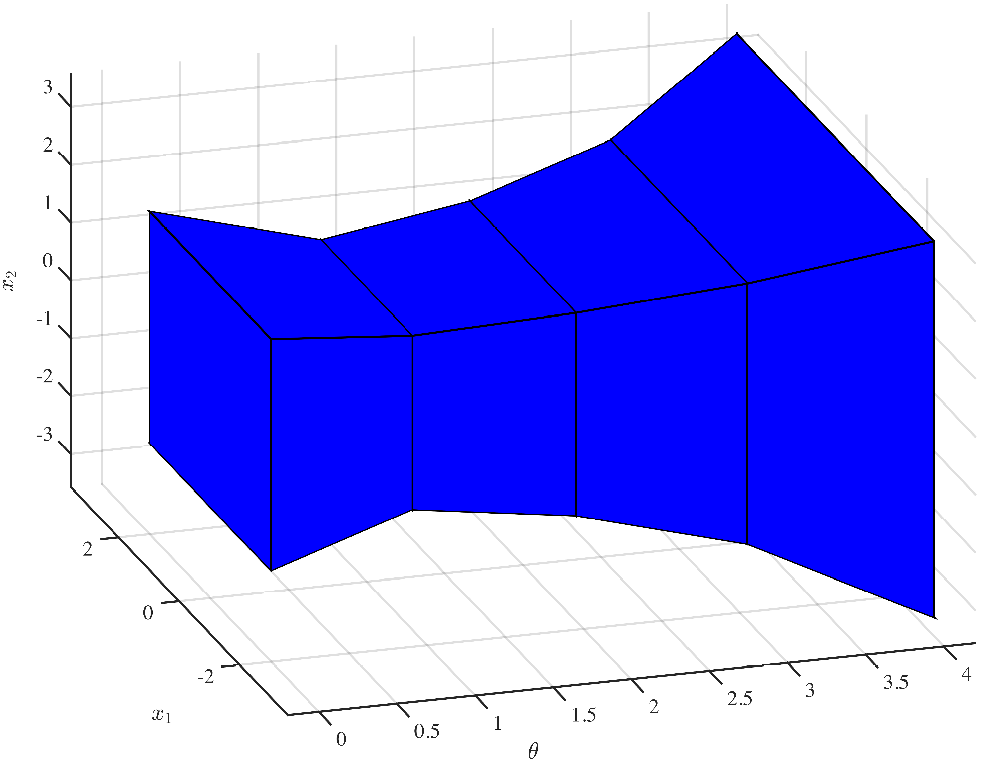
\includegraphics[width=.7\textwidth]{ParametricConvexSet}
\caption[A parametrically convex set.]{The piecewise affine parametric set $\mathcal X(\theta)$ 
defined by $\mathcal X(\theta)\mathrel{\mathop:}=\left\{x:\norm{x}_\infty\leq\max\{-\frac{1}{2}
\theta+2,\frac{1}{4}\theta+\frac{1}{5},\frac{1}{2}\theta+\frac{3}{4},\theta-\frac{3}{4}\}\right\}$ 
for $\theta\in[0,4]$. $\mathcal X(\theta)$ is parametrically convex in~$\theta$.}
\label{fig:parametrically:convex:set}
\end{figure}
%
Notice that Definition~\ref{def:parametric:convexity} does not require convexity of~$\mathcal W(p)$ for all
$p\in X$, we will however only treat maps~$\mathcal W$ for which $\mathcal W(p)$ is convex.
%
In order to compute maximal positive invariant sets for the considered system we need to generalise
the Pontryagin set difference (see e.g.~\cite{blanchini:2007}) to accommodate parametrically convex sets.
%
\begin{defn}[Parametric Pontryagin Difference]\label{def:parametric:pontryagin:difference}
	Let $S\subseteq X$ and let $\mathcal W:X\to\mathcal P(X)$ be a continuous point-to-set map such that
	$\mathcal W(p)$ is convex for all $p\in X$, then the \emph{parametric Pontryagin difference} 
	$S\ominus \mathcal W(S)$ is 
	\begin{equation}\label{eq:definition:parametric:pontryagin:difference}
		S\ominus \mathcal W(S) = \left\{x\in X: \{x\} \oplus \mathcal W(x)\subseteq S\right\},
	\end{equation}
	where $\mathcal W(S)$ denotes the image of $S$ under the map $\mathcal W$. 
\end{defn}
%
At first it may seem sensible to generalise the Pontryagin difference even further and define
%
\begin{equation}\label{eq:extended:parametric:pontryagin:difference}
\begin{split}
	S\ominus \mathcal W(R) &= \{x:\{x\}\oplus \mathcal W(r)\subseteq S\,\forall\, r\in R\}\\
	&=\{x:\{x\}\oplus\bigcup_{r\in R} \mathcal W(r)\subseteq S\}.
\end{split}
\end{equation}
%
However, since $\bigcup_{r\in R} \mathcal W(r)$ may or may not be convex, we can not make any useful
statements about $S\ominus \mathcal W(R)$. 
%
In the case that~$\mathcal W(p)$ is constant, i.e. $\bigcup_{p\in X}\mathcal W(p)=\mathcal W(p)=:C$,
we see that $S\ominus \mathcal W(S)=S\ominus C$ which is the Pontryagin difference for regular sets.
%
For the parametric Pontryagin difference of a convex set and a parametrically convex map we 
have the following result.
%
\begin{thm}\label{thm:convexity:of:pontryagin:difference}
  Let $S\subseteq X$ be a convex set and let $\mathcal W:X\rightarrow\mathcal P(X)$ be a parametrically convex point-to-set
  map such that $\mathcal W(p)$ is convex for all $p\in X$, then $S\ominus \mathcal W(S)$ is convex.
\end{thm}
%
\begin{proof}
To prove the convexity of $ Z :=  S\ominus \mathcal W( S)$ we pick any $z_1,z_2\in Z$, then
by definition of the parametric Pontryagin difference, we have
%
\begin{equation}
	\{z_i\} \oplus \mathcal W(z_i) \subseteq S,\; i=1,2.
\end{equation}
%
To see that $ Z$ is convex we show that line segments between
all possible $z_1$ and $z_2$ are subsets of $ Z$, i.e.~for all $\lambda \in [0,1]$,
\begin{equation}
\begin{aligned}
	\{ \lambda z_1 + (1-&\lambda)z_2
	\}\oplus \mathcal W\left( \lambda z_1 + (1-\lambda)z_2\right)\\
	\subseteq&\left\{ \lambda z_1 + (1-\lambda)z_2
	\right\}\oplus \lambda \mathcal W(z_1) \oplus (1-\lambda)
	\mathcal W(z_2)\\
	\subseteq &\lambda\underbrace{(\{z_1\}\oplus \mathcal W(z_1))}_{\subseteq S}\oplus
	(1-\lambda)\underbrace{(\{z_2\}\oplus \mathcal W(z_2))}_{\subseteq S}\\
	\subseteq& Z
\end{aligned}
\end{equation}
%
where the last inclusion follows from the convexity of $\mathcal S$.
\end{proof}
%
% Now consider a parametrically convex set of the form
% %
% \begin{equation}\label{eq:parametric:polyhedron}
% 	T(s)=\{t:Gt\leq H(s)\},
% \end{equation}
% %
% where each row of $H(s)$ is a convex function in $s\in S$, i.e. each element $H_i(s)$ of 
% $H(s)$ satisfies $H_i(\lambda s_1+(1-\lambda)s_2)\leq \lambda H_i(s_1)+(1-\lambda)H_i(s_2)$ 
% for all $\lambda\in[0,1]$ and $s_1, s_2\in S$. 
% %
% We will use sets for which $H(s)$ is piecewise affine in $s\in S$, i.e. sets
% for which $H_i(s) = \max_k\{f_k s + g_k\}$.
% %
% For sets of this type we have the following result.
% %
% \begin{thm}\label{thm:convex:parametric:set}
%   The point-to-set map $T(s)$ defined by~\eqref{eq:parametric:polyhedron} is parametrically 
%   convex for all $s\in S$ if $H(s)$ is elementwise convex in $s\in S\subseteq X \subset 
%   \mathbb R^n$.
% \end{thm}
% %
% \begin{proof}
% To show that $T(\lambda s_1 + (1-\lambda)s_2)\subseteq \lambda T(s_1) \oplus(1-\lambda)
% T(s_2)$ for all $\lambda \in [0,1]$ and $s_1, s_2\in S$ we note that
% %
% \begin{equation}
% \begin{aligned}
%   T&(\lambda s_1 + (1-\lambda)s_2)\\
%   =& \{t:\; G t \leq H(\lambda s_1 + (1-\lambda)s_2)\}\\
%   \subseteq& \{t:\;Gt\leq\lambda H(s_1)+(1-\lambda) H(s_2)\}\\
%   =&\{t:\;Gt\leq\lambda H(s_1)\}\oplus\{t:\;Gt\leq(1-\lambda)H(s_2)\}\\
%   =&\lambda T(s_1)\oplus(1-\lambda) T(s_2).
%   \end{aligned}
% \end{equation}
% %
% \end{proof} 
% %
% Notice that rays and vertices of $T(s)$ as defined in~\eqref{eq:parametric:polyhedron} will
% be linear combinations of $H_i(s)$, this implies that for piecewise affine $H(s)$ rays
% and vertices $t_k(s)$ will themselves be piecewise affine in $s\in S$, we will exploit
% this fact later on.
%
%
In the following we derive a property for piecewise affine parametric set-valued maps that will
allow convenient computation, namely that it is sufficient to check the number of vertices of 
instances $\mathcal W(p)$ on the boundaries of the parameter space to guarantee the parametric convexity.
%
The statement is summarised in Corollary~\ref{thm:p:convexity:PWA:set:constant:num:verts} in this section.
%
First we introduce the \emph{graph} of $\mathcal W$
%
\[
	\mathscr G(\mathcal W) = \{(p,x) \in\mathbb R^{d+n}: x\in\mathcal W(p)\},
\]
%
its \emph{interior}
%
\[
	\text{int}(\mathscr G(\mathcal W)) = \{(p,x) \in\mathbb R^{d+n}: \forall d\in\mathbb R^n\;\exists 
	\epsilon>0 : x+\epsilon d\in \mathcal W(p)\}
\]
%
and its \emph{boundary}
\[
	\partial \mathscr G(\mathcal W) = \mathscr G(\mathcal W)\setminus \textup{int}(\mathscr G(\mathcal W)).
\]
%
We define the \emph{extended normal cone} as
%
\[
	\mathcal N\mathcal W(p,x) = \{d\in\mathbb R^n: x+\epsilon d \not\in \mathcal W(p)\; \forall \epsilon>0\}
\]
for all $(p,x)\in\partial\mathscr G(\mathcal W)$.
%
\begin{rem}
%
Notice that we define the extended normal cone without an inner product. 
%
The way it is defined here, the conventional normal cone (e.g.~\cite{Boyd:04}) for a convex set $\mathcal C$
%
\[
	N_{\mathcal C}(x) = \{y: \langle y,x-z\rangle\geq0\;\forall z\in\mathcal C\}
\]
%
is be contained in the extended normal cone
%
\[
	\mathcal N_{\mathcal C}(x) = \{y:\exists\epsilon>0\;x+\epsilon y\not\in\mathcal C\}.
\]
%
Furthermore, we have that $\langle d, y\rangle\geq0$ for all $d\in\mathcal N_{\mathcal C}(x), y\in N_{\mathcal C}(x)$.
%
\end{rem}
%
\begin{rem}
%
Notice further that all definitions above are defined relatively for the \emph{set variable} $x$ rather than for graph
variable $(p,x)$.
%
\end{rem}
%
We state the central theorem to connect parametric convexity of a set valued map $\mathcal W$ with properties of its graph
$\mathscr G(\mathcal W)$.
%
\begin{thm}\label{thm:p:convexity:graph}
The map $\mathcal W$ is parametrically convex iff for all $(p_1,x_1),(p_2,x_2)\in\partial\mathscr G(\mathcal W)$
with $\mathcal N\mathcal W(p_1,x_1)\cap\mathcal N\mathcal W(p_2,x_2)\neq\emptyset$ and $p_1\neq p_2$ 
%
\begin{equation}\label{eq:graph:def:p:convexity}
\lambda (p_1,x_1) + (1-\lambda) (p_2,x_2) \not\in\textup{int} (\mathscr G(\mathcal W))
\end{equation}
%
holds for all $\lambda\in(0,1)$.
%
\end{thm}
%
\begin{proof}
%
Assume~\eqref{eq:graph:def:p:convexity} holds for $(p_1,x_1),(p_2,x_2)\in\partial\mathscr G(\mathcal W)$.
%
Then the Minkowski functional (see e.g.~\cite{Rudin:91}) yields $\mu(\mathcal W(\lambda p_1 + (1-\lambda)p_2),
\lambda x_1+(1-\lambda)x_2)\geq1$,
i.e. all interpolation points lie either on the boundary or outside the set $\mathcal W(\lambda p_1+(1-\lambda)p_2)$
therefore the set of all possible interpolation points 
%
\[
	\lambda \mathcal W(p_1)\oplus (1-\lambda)\mathcal W(p_2) = \{x:x=\lambda x_1 + (1-\lambda) x_2 \wedge x_1\in\mathcal 
	W(p_1) \wedge x_2\in\mathcal W(p_2)\}
\]
%
contains the set $\mathcal W(\lambda p_1 + (1-\lambda)p_2)$.
%
Now assume $\mathcal W$ is parametrically convex but~\eqref{eq:graph:def:p:convexity} is not satisfied for 
some $(p_1,x_1),(p_2,x_2)\in\partial\mathscr G(\mathcal W)$ with $\mathcal N\mathcal W(p_1,x_1)\cap\mathcal 
N\mathcal W(p_2,x_2)\neq\emptyset$, i.e. $\lambda x_1 + (1-\lambda)x_2\in\text{int}(\mathcal W(\lambda p_1 + 
(1-\lambda)p_2)$.
%
This implies that a full dimensional ball $B_\epsilon(x ) = \{y:\| 
x-y\|<\epsilon\}$
is contained in $\mathcal W(\lambda p_1 + (1-\lambda)p_2)$, i.e. $B_\epsilon(\lambda x_1 + (1-\lambda)x_2 )\subset
\mathcal W(\lambda p_1 + (1-\lambda)p_2)$ for some $\epsilon>0$.
%
Since $\mathcal N\mathcal W(p_1,x_1)\cap\mathcal N\mathcal W(p_2,x_2)\neq\emptyset$, there exist directions 
$d\in\mathcal N\mathcal W(p_1,x_1)\cap\mathcal N\mathcal W(p_2,x_2)$ which can not be represented as $d=\lambda d_1+
(1-\lambda)d_2$ with $x_1 + \epsilon d_1\in\mathcal W(p_1)$ and $x_2  + \epsilon d_2\in\mathcal W(p_2)$, however since $B_\epsilon$ is full dimensional
all directions exist, $x+\epsilon d\in\mathcal W(\lambda p_1 + (1-\lambda)p_2)$.
%
Hence, $\mathcal W$ can not be parametrically convex.
\end{proof}

\begin{rem}
Notice that condition~\eqref{eq:graph:def:p:convexity} is a non-convexity condition on the graph $\mathscr G(\mathcal W)$.
%
If $\mathscr G(\mathcal W)$ is strictly convex anywhere~\eqref{eq:graph:def:p:convexity} is violated and 
$\mathcal W$ can not be parametrically convex.
\end{rem}
%
\begin{rem}
%
Furthermore notice that the condition on the extended normal cones is only a restriction on the choice of 
$(p,x)$.
%
It is to avoid choices such that the entire line between $(p_1,x_1)$ and $(p_2,x_2)$ is contained in the interior
of the graph by convexity of $\mathcal W(p_i)$.
%
\end{rem}
%
\begin{figure}
\centering 
\begin{lpic}{pConvexSetsAbstract}
\lbl{74,16;$p$}
\lbl{52,20,90;$\mathcal W(p_2)$}
\lbl{10,20,90;$\mathcal W(p_1)$}
\lbl[bl]{17,35,45;$\mathcal N\mathcal W(p_1,x_1)$}
\lbl[bl]{58,37,45;$\mathcal N\mathcal W(p_2,x_2)$}
\lbl[bl]{62,17,45;$\textup{int}(\mathscr{G}(\mathcal W))$}
\lbl[l]{77,4;$\partial \mathscr{G}(\mathcal W)$}
\end{lpic}
\caption[Example p-convex set]{Illustration of the concepts for a scalar parametrically convex map in one-dimension.}
\end{figure}
%
\begin{korr}
%
Let $\mathcal W(p):=\{x\in\mathbb R^n: r(p,x)\leq0\}$ define a set-valued map with a continuous function 
$r: \mathbb R^d \times\mathbb R^n \rightarrow \mathbb R,(p,x)\mapsto r(p,x)$, then $\mathcal W$ is parametrically
convex iff the function $r$ is concave in $p\in\mathbb R^d$ and convex in $x\in\mathbb R^n$.
%
\end{korr}
%
\begin{proof}
The convexity in $x\in\mathbb R^n$ is required to satisfy the requirement that $\mathcal W(p)$ is convex
for all fixed values of $p\in\mathbb R^d$. 
%
Assume that for some region $\Omega\subset\mathbb R^d$ the function $r(\cdot,x)$ is non-concave (i.e. 
strictly convex), any convex subset $\mathcal C\subseteq\Omega$ will hence be such that $\mathscr 
G(\mathcal W)\vert_{\mathcal C}$ is a convex set.
%
In particular all lines between all $(p_1,x_1),(p_2,x_2)\in \partial\mathscr G(\mathcal W)\vert_{\mathcal C}$ will satisfy
$\lambda (p_1,x_1) + (1-\lambda) (p_2,x_2) \in\textup{int} (\mathscr G(\mathcal W))\vert_{\mathcal C}$ since
$\mathscr G(\mathcal W)\vert_{\mathcal C}$ is strictly convex in $p$.
%
This implies that $r(\cdot,x)$ can not be non-concave in any non-trivial set $\Omega\subseteq\mathbb R^d$ and still
be parametrically convex.
\end{proof}
%
\begin{korr}\label{thm:polytopic:set:not:p:convex}
The polytopic parametric set valued map $\mathcal W(p):=\{x: a_i x + b_i p\leq c_i \forall i\leq m\}$ is not parametrically convex for 
any non-trivial matrix $B$.
\end{korr}
%
\begin{proof}
The graph $\mathscr G(\mathcal W)$ is given by
%
\begin{equation*}
	\mathscr G(\mathcal W) = \{(p,x):a_i x + b_i p\leq c_i \forall i\leq m\}
\end{equation*}
%
and hence is a convex set and violates Theorem~\ref{thm:p:convexity:graph}.
\end{proof}
%
We now can prove the following central corollary.
%
\begin{korr}\label{thm:p:convexity:PWA:set:constant:num:verts}
The piecewise affine polytopic parametric set valued map 
%
\begin{equation}\label{eq:definition:PWA:polytopic:set:general}
	\mathcal W(p) := \left\{x: a_i x \leq \max_{k\leq l}\{b_{i,k} + C_{i,k}p\},i\leq m\right\}
\end{equation}
%
is parametrically convex iff the number of vertices $v_i(p)$ and rays $u_i(p)$ is constant.
\end{korr}
%
\begin{proof}
For clarity this proof is divided in 3 parts:
\begin{enumerate}
\item Notice that $h_i(p) = \max_{k\leq l} \{b_{i,k} + C_{i,k}p\}$ is a multi-parametric linear program (mpLP),
its solution is a piecewise affine function $h_i(p) = b_{i,k^\ast_i} + C_{i,k^\ast_i}p$ where $k^\ast_i(p)$ is constant
inside a polytopic complex, see e.g.~\cite{spjotvold:2005}.
%
That means that there exists a finite partitioning $\mathbb R^d = \bigcup_{i\leq t} \mathcal P_i$ with convex polyhedra 
$\mathcal P_i$ such that ${\bf{k}}^\ast\vert_{\mathcal P_i} = (k_1^\ast,\dots,k_m^\ast) = const$.
%
A standard degeneracy assumption is that in neighbouring partitions ${\bf{k}}^\ast\vert_{\mathcal P_i}$ and 
${\bf{k}}^\ast\vert_{\mathcal P_j}$ differ in exactly one element.
%
This partitioning implies that the graph $\mathscr G(\mathcal W)$ is given as a finite union of polyhedra
%
\begin{equation*}
	\mathscr G(\mathcal W) = \bigcup_{j\leq t} \left\{x: a_i x \leq b_{i,k_i^\ast} + C_{i,k_i^\ast}p,i\leq m
	\right\}\bigr\vert_{\mathcal P_j}
\end{equation*}
%
But this implies that if the number of vertices or rays changes in any partition $\mathcal P_i$ then $\mathscr
G(\mathcal W)\vert_{\mathcal P_i}$ is a strictly convex polytope and theorem~\ref{thm:polytopic:set:not:p:convex} applies.
%
\item Our attention hence is concentrated to the boundaries of the partitions $\mathcal P_i$.
%
These are the points $\mathcal P_i \cap \mathcal P_j$ where some mpLP changes its solution, i.e. 
$b_{i,k_{i_1}^\ast} + C_{i,k_{i_1}^\ast} p = b_{i,k_{i_2}^\ast} + C_{i,k_{i_2}^\ast} p$.
%
Notice that a vertex $v_i(p)$ is given by \emph{active} and \emph{inactive} inequalities, i.e. $\mathcal A_i(p)$ and
$\mathcal I_i(p) = \{1,\dots,m\}\setminus\mathcal A_i(p)$ respectively.
%
\begin{equation*}\begin{split}
	a_j v_i(p) &= b_{j,k_j^\ast} + C_{j,k_j^\ast} p \quad\forall j\in\mathcal A_i(p)\\
	a_j v_i(p) &< b_{j,k_j^\ast} + C_{j,k_j^\ast} p \quad\forall j\in\mathcal I_i(p)
\end{split}\end{equation*}
%
In order for the number of vertices to change, there must be a hyperplane $fp=g$, such that the number of vertices for $fp<g$ is 
$N$ and for $fp>g$ is at least $N+1$.
%
It follows from the previous discussion that $\{p:fp=g\} = \textup{aff}\{\mathcal P_i\cap\mathcal P_j\}$ for some $i\neq j$.
%
For vertices $v_i(p)$ and $v_j(p)$ to merge the index sets $\mathcal A_i(p)$ and $\mathcal A_j(p)$ have to differ in only one 
element, i.e. $\mathcal A_i(p) = \mathcal J\cup \{s\}$ and $\mathcal A_j(p) = \mathcal J\cup\{u\}$ for $fp>g$.
%
Furthermore, for $p$ with $fp\leq g$ we have $v_i(p)=v_j(p)$, this implies $\mathcal A_i(p) = \mathcal A_j(p)$.
%
Since only one alteration of the active index set is considered (due to generic assumptions), the active set $\mathcal A_i(p) = \mathcal A_j(p)
= \mathcal J \cup \{s,u\}$.
%
Hence on the hyperplane $fp=g$ both, the maximising index ${\bf{k}}^\ast(p)$ and the active index sets $\mathcal A_i(p)$ 
and $\mathcal A_j(p)$ change, which is degenerate.
%
\item In order for the degenerate graph $\mathscr G(W)$ to be parametrically convex the overdetermined vertex $v_i(p)=v_j(p)$
have to be identical, in particular their dependence on $p$ has to be identical.
%
This can be expressed with the implicit function theorem:
%
\begin{equation*}\begin{split}
	\frac{d}{dp}\left(	A_{\mathcal J\cup \{s\}} v_i(p) - b_{\mathcal J\cup \{s\}} - C_{\mathcal J\cup \{s\},{\bf{k}}^\ast} p\right) &= 0\\
	\frac{d}{dp}\left(	A_{\mathcal J\cup \{u\}} v_i(p) - b_{\mathcal J\cup \{u\}} - C_{\mathcal J\cup \{u\},{\bf{k}}^\ast} p\right) &= 0
\end{split}\end{equation*}
%
which leads to 
%
\begin{equation*}\begin{split}
	A_{\mathcal J\cup \{s\}} \frac{dv_i}{dp} &= C_{\mathcal J\cup \{s\},{\bf{k}}^\ast}\\
	A_{\mathcal J\cup \{u\}} \frac{dv_i}{dp} &= C_{\mathcal J\cup \{u\},{\bf{k}}^\ast}
\end{split}\end{equation*}
%
since we can assume that the inequalities are non-redundant for some right hand side, we obtain that 
%
\begin{equation}\label{eq:derivative:condition:on:index:sets}
	\frac{dv_i}{dp} = A_{\mathcal J\cup \{s\}}^{-1}C_{\mathcal J\cup \{s\},{\bf{k}}^\ast} = 
	A_{\mathcal J\cup \{u\}}^{-1}C_{\mathcal J\cup \{u\},{\bf{k}}^\ast}
\end{equation}
%
has to hold for the degenerate graph to remain parametrically convex.
%
Notice that~\eqref{eq:derivative:condition:on:index:sets} is again a degenerate condition, since arbitrarily small perturbations
will produce different behaviour.
\end{enumerate}
\end{proof}
%
\begin{rem}
Corollary~\ref{thm:p:convexity:PWA:set:constant:num:verts} is essential for numerical examples, as it can be reformulated to:
%
The set valued map defined by~\eqref{eq:definition:PWA:polytopic:set:general} is parametrically convex iff it has a constant 
number of vertices throughout the parameter space~$X$.
%
\\[1em]
%
Since the map is continuous it is sufficient to verify this at the vertices of the parameter space.
%
\end{rem}
%
To illustrate the effects of perturbations to a degenerate piecewise affine map, consider the following low dimensional 
examples:
%
\begin{quote}
Let $\mathcal W_i(p)$ be defined by
%
\begin{equation*}\begin{split}
	\mathcal W_1(p) = \left\{x : \left(\begin{array}{cc}
	1&1\\
	-1&1\\
	0&1\\
	0&-1 
	\end{array}\right)x \leq \left(\begin{array}{c}
	\max\{1+p,\frac{1}{2}+2p\} \\
	\max\{1+p,\frac{1}{2}+2p\} \\
	\frac{1}{2}+2p \\
	1
	\end{array}\right)
	\right\}\\
%
	\mathcal W_2(p) = \left\{x : \left(\begin{array}{cc}
	1&1\\
	-1&1\\
	0&1\\
	0&-1 
	\end{array}\right)x \leq \left(\begin{array}{c}
	\max\{1+p,\frac{1}{2}+(2+\epsilon)p\} \\
	\max\{1+p,\frac{1}{2}+2p\} \\
	\frac{1}{2}+2p \\
	1
	\end{array}\right)
	\right\}\\
%
	\mathcal W_3(p) = \left\{x : \left(\begin{array}{cc}
	1&1\\
	-1&1\\
	0&1\\
	0&-1 
	\end{array}\right)x \leq \left(\begin{array}{c}
	\max\{1+p,\frac{1}{2}+\epsilon+2p\} \\
	\max\{1+p,\frac{1}{2}+2p\} \\
	\frac{1}{2}+2p \\
	1
	\end{array}\right)
	\right\}
	\end{split}
\end{equation*}
%
%
\begin{figure}
\begin{center}
\subfigure[$\mathcal W_1(p)$]{\includegraphics[width=.45\textwidth]{pConvDegenerateSet}}
\subfigure[$\mathcal W_2(p)$]{\includegraphics[width=.45\textwidth]{pConvPertInLinTerm}}\\
\subfigure[$\mathcal W_3(p)$]{\includegraphics[width=.45\textwidth]{pConvPertInConstantTerm}}
\end{center}
\caption[Degenerate PWA p-convex sets]{For $\mathcal W_1(p)$ the right hand side was chosen in order 
to satisfy~\eqref{eq:derivative:condition:on:index:sets} 
and for the graph to be degenerate. For both $\mathcal W_{2,3}(p)$ there is no drop in number of vertices for different 
$p\in[-1,\infty),\epsilon=10^{-1}$.}
\label{fig:degenerate:PWA:set:and:comparison}
\end{figure}
%
See figure~\ref{fig:degenerate:PWA:set:and:comparison} for an illustration.
\end{quote}
%
%
%
%
%
\section{Example}\label{sec:example:linearisation:error:as:state:dependent:constraint}
In this section we derive a disturbance set that is of the form~\eqref{eq:derivative:condition:on:index:sets}
with a piecewise affine right hand side~$H(s)$. 
%
Consider a discrete time nonlinear system of the form
%
\begin{equation}
	x^+ = f(x,u)
\end{equation}
%
with $x_e=f(x_e,u_e)$ as an equilibrium point. 
%
Close to the equilibrium point the dynamics can be approximated by ${\tilde x}^+ = A \tilde x 
+ B\tilde u$ with $\tilde x = x-x_e$ and $\tilde u = u - u_e$ and the linearisation matrices
$A = \frac{\partial f}{\partial x}\vert_{(x_e,u_e)}$ and $B = \frac{\partial f}{\partial u}
\vert_{(x_e,u_e)}$.
%
We want to describe the dynamics of the nonlinear system with those of its linearisation considering
an additive disturbance. 
%
I.e. we want that for all $x\in X_c$ and $u\in U_c$ there exists a realisation 
$v\in V(x,u)$ such that the identity $f(x,u)=Ax + B u + v$ holds. 
%
In order to derive a parametrised set $V(x,u)$ such that the desired identity holds we use
the mean value theorem (see e.g.~\cite{Apostol:1974}):
%
\begin{thm}[Mean Value Theorem]\label{thm:mean:value:theorem}
Let $g : \mathcal X \rightarrow\mathbb R^m$ be continuously
differentiable, $\mathcal X\subset\mathbb R^n$ be open,
and $x \in\mathcal X$, $h \in\mathbb R^n$ be such that 
$x + th \in\mathcal X$ for all $t\in [0 ,1]$. Then
\begin{equation}
	g(x+h) = g(x) + \left(\int_0^1 \frac{\partial g}{\partial x}(x+th)dt\right)\cdot h.
\end{equation}
\end{thm}
%
We can use this to state
%
\begin{equation}
\begin{split}
	f(x_e+x,u_e+u)-A(x_e+x)-B(u_e+u) = \underbrace{f(x_e,u_e) - A x_e - B u_e}_{=0} \\
	+ \int_0^1\left(\frac{\partial f}{\partial x}(x_e+tx,u_e+tu) \cdot x + 
	\frac{\partial f}{\partial u}(x_e+tx,u_e+tu) \cdot u \right) dt -Ax-Bu\\
	= \underbrace{\left(\int_0^1 \frac{\partial f}{\partial x}(x_e+tx,u_e+tu) dt - A\right)}_{H^x} x + 
	\underbrace{\left(\int_0^1 \frac{\partial f}{\partial u}(x_e+tx,u_e+tu) - B \right)}_{H^u} u.
\end{split}
\end{equation}
%
This means that for any given $(x,u)\in X\times U$ we can compute an additive disturbance $v=H^x x + H^u u$
such that $f(x_e+x,u_e+u)-Ax-Bu = v$.
%
Assume we had all possible $H^x$ and $H^u$ for all $(x,u)\in X\times U$ given, clearly then 
$\min\{H^x x + H^u u\} \leq f(x_e+x,u_e+u)-Ax-Bu \leq \max\{H^x x + H^u u\}$ holds true.
%
For general nonlinear systems there is no way to obtain an analytic solution for $H^x$ and $H^u$,
so instead $K$ samples of $X\times U$ have to be used to obtain a description of 
the disturbance set
%
\begin{equation}\label{eq:derivation:of:PWA:disturbance:set}
\begin{split}
	V^K(x,u) &= \left\{v: \min_{k\leq K}\{H^x_k x + H^u_k u\} \leq v \leq \max_{k\leq K}\{H^x_k x + H^u_k u\} \right\}\\
	&= \left\{v: v \leq \max_{k\leq K}\{H^x_k x + H^u_k u\} \wedge -v \leq \max_{k\leq K}\{-H^x_k x - H^u_k u\} \right\}
\end{split}
\end{equation}
%
Notice that sampling the set $\gimel(x,u) = \left\{v : \min\{H^x x + H^u u\} \leq v \leq \max\{H^x x + H^u u\}\right\}$ 
leads to an inner approximation which is convexified by taking its convex hull.
%
The set $V^K(x,u)$ as defined in~\eqref{eq:derivation:of:PWA:disturbance:set} is of the
type~\eqref{eq:derivative:condition:on:index:sets} with a piecewise linear right hand side. We may
want to add a constant term to accommodate model uncertainties.
%
%
%
%
\section{Maximal Positive Robust Invariant Sets}\label{sec:parametrised:MRPI:set}
In this section we present a way to calculate maximal robust positive invariant sets for
linear discrete time systems under the influence of additive perturbation.
%
We assume the perturbation to be constrained in sets which are piecewise affine in
the state, i.e.
%
\begin{equation}\label{eq:definition:PWA:uncertainty}
v\in \mathcal V(x) = \left\{v: Gv\leq\max_k\{H_k^x x + h_k\}\right\}.
\end{equation}
%
The definition of the maximal robust positive invariant set in this scenario is given as
the largest set satisfying
%
\begin{equation}\label{eq:MRPI:state:dependent:disturbance}
	\mathcal X^\infty = \left\{x: \Psi x + v \in\mathcal X^\infty\,\forall\, v\in\mathcal V(x)\right\},
\end{equation}
%
largest in the sense that it includes all smaller ones.
%
The implicit definition of~\eqref{eq:MRPI:state:dependent:disturbance} suggests a recursive 
computation of $\mathcal X^\infty$.
%
We assume system dependent state constraints $\mathscr X\subseteq\mathbb R^n$ are given,
we furthermore assume that $\mathscr X$ is polyhedral and contained in a band.
%
\begin{defn}[Band Property]
We say that a set $X\subseteq\mathbb R^d$ possesses the band property if there exists a 
matrix~$\Gamma\in\mathbb R^{p\times d}$ such that $X\subseteq B = \{x:\Gamma x\leq {\bf{1}}\wedge
-\Gamma x\leq{\bf{1}}\}.$
\end{defn}
%
That is, we assume that $\mathscr X= \{x:\Lambda_i x \leq \lambda_i \forall\, i\leq m\}\subseteq\{x:\Gamma x\leq{\bf{1}}\wedge
-\Gamma x\leq{\bf{1}}\}=:\mathscr B$.
%
In the following we discuss how to apply the principle of the Kolmanovsky and Gilbert 
algorithm\footnote{The concept was first introduced for 
unperturbed systems in 1991 by Gilbert and Tan~\cite{Gilbert:1991}, therefore all its derivatives 
are also referred to as the \emph{Gilbert and Tan algorithms}.} 
presented in~\cite{Kolmanovsky:1995}.
%
The algorithm is a recursive iteration: Starting from $\mathscr X$ we 'cut off' all such stated 
for which the successor state would violate~\eqref{eq:MRPI:state:dependent:disturbance}, i.e.
in the $n^\text{th}$~iteration we introduce constraints which enforce that the trajectories
of all points in the set would remain in the set for $n$~time steps.
%
This means that in the first iteration we enforce that for all points in the iterate the 
successor state is contained in the initial set $x^+\in X_0 = \mathscr X$:
%
\begin{equation}\label{eq:PWA:disturbance:first:iterate}
\begin{split}
	X_1 &= \{x: \Psi x + v\in X_0 \forall v\in\mathcal V(x)\}\\
	&=\{x:\Lambda_i(\Psi x +v)\leq \lambda_i \forall\,i\leq m_0\}\\
	&=\left\{x:\Lambda_i\Psi x + 
	\underbrace{\left\{\begin{array}{rl}\max& \Lambda_i v\\ 
	\text{s.t.}& v\in\mathcal V(x)
	\end{array}\right\}}_{\gamma_{1,i}^\ast(x)} \leq \lambda_i \forall\,i\leq m_0\right\}
\end{split}
\end{equation}
This requires the solution $m_0$ multi-parametric linear programs\footnote{Multi-parametric 
linear programs have been introduced as optimisation problems
in the late 1958 by~\cite{Courtillot:1958}. Various ways to solve mpLPs have been proposed.}
(mpLPs) in order to obtain~$v_{1,i}^\ast(x)$.
%
However, the solution of multi-parametric linear programs will be given by vertices 
of the constraint set, i.e. $\gamma_{1,i}^\ast(x)=\Lambda_i v_{k^\ast}(x)$ where $v_{k^\ast}(x)$
is the optimising vertex.
%
Recall that since $\mathcal V(x)$ is piecewise affine in $x$ its vertices will also be piecewise 
affine in $x$, i.e. there exists a representation $v_k(x)=\max_{l\leq K_k}\{W_l^k x + w_l^k\}$.
%
Notice that we do not need to solve all mpLP in order to compute $X_1$, adding all available
$W_l,w_l$ produces the desired set without solving $m_0$ mpLP:
%
\begin{equation}\label{eq:derivation:of:row:reduction:instead:of:mpLP}
\begin{split}
	X_1 &= \{x: \Lambda_i\Psi x + \gamma_{1,i}^\ast(x)\leq\lambda_i \,\forall i\leq m_0 \}\\
	&= \left\{x: \Lambda_i\Psi x + \max_l\{\Lambda_i (W_l^{k^\ast} x + w_l^{k^\ast}) \} \leq \lambda_i\, 
	\forall i\leq m_0 \right\} \\
	&= \left\{x: (\Lambda_i\Psi + \Lambda_i W_l^{k^\ast}) x \leq \lambda_i-\Lambda_i w_l^{k^\ast}\,
	\forall i\leq m_0, l\leq K_k  \right\} \\
	&= \left\{x: (\Lambda_i\Psi + \Lambda_i W_l^k) x \leq \lambda_i - \Lambda_i w_l^k\,
	\forall i\leq m_0, l\leq K_k, k\leq \kappa \right\}.
\end{split}
\end{equation}
%
The equalities~\eqref{eq:derivation:of:row:reduction:instead:of:mpLP} hold since only the 
inequalities which define~$\gamma_{1,i}^\ast(x)$ will define the set~$X_1$, i.e. we avoid
solving mpLP by introducing redundant inequalities, instead of $m_0$ supporting hyperplanes
we describe the set by $m_1 = m_0\cdot \kappa\cdot \prod_{k\leq \kappa} K_k$ hyperplanes with
a large number of them being redundant, here~$\kappa$ denotes maximal the number of vertices 
of~$\mathcal V(x),\,x\in\mathscr X$.
%
This seems to be a poor trade off, however, we can use inequality reduction algorithms at any
point of the iteration and reduce the number of hyperplanes~$m_1$ in the representation of~$X_1$.

The next set iterate~$X_2$ is then defined by
%
\begin{equation}
	\begin{split}
	X_2 &= \left\{x: \Psi (\Psi x + v) + \tilde v\in X_0\,\forall v,\tilde v\in\mathcal V(x) \right\}\\
	&= \{x\in X_1 : \Psi x + v \in X_1\,\forall v\in\mathcal V(x)\}\\
	&= X_1 \cap \{x: \Psi x + v \in X_1\,\forall v\in\mathcal V(x)\},
	\end{split}
\end{equation}
%
so that successive set iterates can be defined recursively.
%
The general iterate is given by:
%
\begin{equation}\label{eq:general:MRPI:iteration}
	X_{k+1} = X_k \cap \{x:\Psi x + v\in X_k\, \forall v\in\mathcal V(x)\}
\end{equation}
%
It is obvious that by its definition $X_{k+1}\subseteq X_k$, once $X_k\subseteq X_{k+1}$ holds
the iteration~\eqref{eq:general:MRPI:iteration} terminates.
%
$X_k\subseteq X_{k+1}$ implies that all $x\in X_k$ also satisfy $x\in X_{k+1}$, however
$X_{k+1}$ is defined as points to which the successor state is contained in $X_k$, therefore
$X_{k+1} = \mathcal X^\infty$. 

In the remainder of this section we will prove that the described algorithm terminates 
in a finite number of iterations.
%
Notice that the set iterates defined by~\eqref{eq:general:MRPI:iteration} can be formally
be defined by
%
\begin{equation}
	X_{k+1} = X_k \cap \{x: \Lambda_i\Psi^k x + \sum_{l=1}^{k-1} \gamma_{l,i}^\ast(x)\leq\lambda_i\,
	\forall i\leq m_0\},
\end{equation}
%
where
%
\begin{equation}\begin{split}
	\gamma_{l,i}^\ast(x) &= \max_j \Lambda_i\Psi^{l-1} v_j(x) \\
	&= \begin{array}{rl} \max_v &\Lambda_i\Psi^{l-1} v\\
		\text{s.t.} & v\in\mathcal V(x)\end{array} \\
	&= \begin{array}{rl} \max_{\tilde v} &\Lambda_i \tilde v\\
		\text{s.t.} & \tilde v\in \Psi^{l-1}\mathcal V(x) \end{array}.
\end{split}\end{equation}
%
So that~\eqref{eq:general:MRPI:iteration} becomes
%
\begin{align}
	X_{k+1} &= X_k \cap \left( \Psi^{-k-1} X_0\, \underset{1\leq i\leq k}{\bigominus} 
	\Psi^{i-1}\mathcal V(X_k) \right)\nonumber \\
	&=\bigcap_{l\leq k+1}\left(\Psi^{-l} X_0 \underset{1\leq i\leq l-1}{\bigominus} 
	\Psi^{i}\mathcal V(X_{l-1}) \right). \label{eq:MRPI:recursion:closed:form}
\end{align}
%
The structure of~\eqref{eq:MRPI:recursion:closed:form} is of central importance for the proof
of finite determinability of~$\mathcal X^\infty$.
%
The first statement we can prove is the following:
%
\begin{thm}\label{thm:band:implies:compactness}
Let the system constraints be contained in a band~$\mathscr X\subseteq \mathscr B 
=\{x: \Gamma x\leq{\bf{1}}\wedge -\Gamma x\leq{\bf{1}}\}$, let $0\in\mathcal V(x)$ for all $x\in\mathscr X$ 
and let the pair $(\Psi,\Gamma)$ be observable, then there exists a natural number $N\leq n$ such 
that~$X_N$ is compact.
\end{thm}
%
\begin{proof}
First recall the fact that $\mathcal A\ominus \mathcal B\subseteq\mathcal A$ if $0\in\mathcal B$,
see e.g.~\cite{blanchini:2007}, this fact extends to the parametric Pontryagin difference.
%
Therefore we have
%
\begin{equation}
	X_k= \bigcap_{l\leq k}\left(\Psi^{-l} X_0 \underset{1\leq i\leq l-1}{\bigominus} 
	\Psi^{i}\mathcal V(X_{l-1}) \right) \subseteq \bigcap_{l\leq k} \Psi^{-l} X_0
	= \bigcap_{l\leq k} \Psi^{-l}\mathscr X \subseteq \bigcap_{l\leq k} \Psi^{-l} \mathscr B.
\end{equation}
%
Note that observability of $(\Psi,\Gamma)$ is equivalent to the observability matrix
\[
	\Omega_o = \left(\begin{array}{c}
	\Gamma \\ \Gamma \Psi \\ \vdots \\ \Gamma \Psi^{n-1}
	\end{array}\right)
\]
%
has full rank.
%
This is equivalent to the null space of $\Omega_o$ being trivial, i.e.~$\ker\Omega_o=\{0\}$,
which implies that~$\{x: \Omega_o x \leq {\bf{1}} \wedge -\Omega_o x \leq {\bf{1}}\}$ is bounded.
%
Note further that
\begin{equation}
	X_n \subseteq \bigcap_{k\leq n} \Psi^{-k}\mathscr B = \left\{x:\underset{k\leq n}{\bigwedge} 
	\pm \Gamma\Psi^{k}x\leq{\bf{1}} \right\} =\{x: \Omega_o x \leq {\bf{1}}\wedge -\Omega_o x\leq{\bf{1}} \}.
\end{equation}
%
Therefore we conclude that $X_n$ is contained in a compact set, hence is itself bounded.
%
The case that~$N<n$ is possible for matrices $\Gamma$ with $\text{rank}(\Gamma)>1$.
\end{proof}
%
We can use Lemma~\ref{thm:band:implies:compactness} to prove the following statement:
%
\begin{thm}[\footnote{
	The earliest proof of finite determinability of the proposed algorithm was published 
	in~\cite[Theorem 4.2]{Kolmanovsky:1995}, the assumptions made for Lemma~\ref{thm:band:implies:compactness}
	and~\ref{thm:finite:terminability:MRPI:algorithm} coincide for the case of constant disturbance sets.
	%
	The formulation chosen here is more explicit than the one stated in~\cite{Kolmanovsky:1995}, since
	all conditions are on data available before initialising the algorithm.
	}]
\label{thm:finite:terminability:MRPI:algorithm}
Let the assumptions for Lemma~\ref{thm:band:implies:compactness} hold, let furthermore
$x^+=\Psi x$ be asymptotically stable and let $\mathcal V(x)$ be bounded for all $x\in\mathscr X$, 
then iteration~\eqref{eq:general:MRPI:iteration} with $X_0=\mathscr X$ terminates in a finite 
number of number of steps.
\end{thm}
%
\begin{proof}
Using~\eqref{eq:general:MRPI:iteration} we can easily see that if for some $k>0$
the set iterate $X_k$ is empty that implies that $X_k=\mathcal X^\infty = \emptyset$,
in this trivial case we can easily see that the algorithm terminates after $k$ iterations.
%
For the remainder of this proof we assume that all set iterates are non-empty.

Let $\rho$ denote the spectral radius of $\Psi$, since $\Psi$ is asymptotically
stable we have $\rho<1$.
%
Let $r_1$ be the radius of the largest ball contained in $X_0$ i.e. $\mathcal E(r_1)\subseteq X_0$ 
and let $r_2$ be the radius of smallest ball containing $V(x)$ for all $x\in X_0$.
%
Recall that $X_k = \bigcap_{l\leq k} D_l$, where $D_k$ is defined by
%
\begin{equation}
	D_l = \underbrace{\Psi^{-l} X_0}_{\mathcal S_1} \ominus 
	\underbrace{\left(\bigoplus_{1\leq i\leq l-1} \Psi^{i}\mathcal V(X_{l-1})\right)}_{\mathcal S_2}
\end{equation}
%
We can easily lower bound $\mathcal S_1$ by using $r_1$: $\mathcal S_1 = \Psi^{-l} X_0 
\supseteq \Psi^{-l}\mathcal E(r_1) \supseteq \mathcal E(\rho^{-l} r_1)$.
%
Recall that $X_l\subseteq X_{l-1}$ and therefore $X_l\subseteq X_0$ for all $l\geq0$.
%
We use this fact to obtain the containment $\mathcal S_2 = \bigoplus_{1\leq i\leq l-1} 
\Psi^{i}\mathcal V(X_{l-1})\subseteq \bigoplus_{1\leq i\leq l-1} \Psi^{i}\mathcal V(X_0)\subseteq
\bigoplus_{1\leq i\leq l-1} \Psi^{i}\mathcal E(r_2)\subseteq\bigoplus_{1\leq i\leq l-1} \mathcal E(\rho^{i} r_2)\subseteq
\mathcal E(\sum_{1\leq i\leq l-1}\rho^i r_2)\subseteq \mathcal E(\frac{1}{1-\rho} r_2)$.
%
In summary we can state that~$D_l$ consists of the exponentially expanding set~$\mathcal S_1$
subtracted by the set~$\mathcal S_2$ which is bounded, therefore~$D_l$ itself expands exponentially,
that is $D_l\supseteq\mathcal E(\rho^{-l} r_1 - \frac{1}{1-\rho} r_2)$.
%
Due to Lemma~\ref{thm:band:implies:compactness} we know that for $N\leq n$ the set iterate~$X_N$ is
bounded, let $r_3$ denote the smallest ball that contains $X_N$.
%
We can conclude that for $l$ such that $X_N\subseteq\mathcal E(r_3)\subseteq\mathcal 
E(\rho^{-l} r_1 - \frac{1}{1-\rho} r_2)\subseteq D_l$ holds the set $D_l$ covers
$X_N$, i.e. intersections with $D_l$ will not change $X_l$.
%
We can therefore give an upper bound on the number of iterations necessary for the algorithm
to terminate, it is given by the smallest integer $M$ such that
\begin{equation}\label{bnd:first:lower:bound:on:iteration:count}
	M\geq \frac{1}{\log(\frac{1}{\rho})}\left(\log\left(r_3+\frac{1}{1-\rho}r_2\right)-\log r_1 \right)
\end{equation}
is satisfied.
\end{proof}
%
Notice that the constants used in~\eqref{bnd:first:lower:bound:on:iteration:count} are not
quite convenient to compute, we can however compute bounds on $r_1,\, r_2$ and $r_3$ using 
singular values.
%
For this let $\bar\sigma(\Gamma)$ and $\underline\sigma(\Gamma)$ denote the maximal and the minimal
singular value of~$\Gamma$ respectively.
%
We know that~$\bar\sigma(\Gamma)\norm{x}\geq\norm{\Gamma x}$ and therefore $\bar\sigma(\Gamma)\norm{x}
\leq \sqrt{n}\Rightarrow \norm{\Gamma x}\leq\norm{\bf{1}}=\sqrt{n}$, that $r_1=\frac{\bar\sigma(\Gamma)}{\sqrt{n}}$
follows form standard result for singular values, see e.g.~\cite{Golub:1996}.
%
We use a similar argument to obtain a bound on $r_3$ before deriving a bound on $r_2$:
%
It is easy to see that the radius of the largest ball containing $X_N$ is given by the maximal
norm of its vertices, i.e. $r_3=\max_{i}\norm{x_i}$ where $x_i$ satisfies $\Omega_{o,\mathscr{A}_i} x_i={\bf{1}}$
and $\Omega_{o,\bar{\mathscr A}_i}x_i<{\bf{1}}$.
%
From this we can deduce that
%
\begin{equation}\begin{split}
	\sqrt{n}=\norm{\bf{1}}=\norm{\Omega_{o,\mathscr{A}_i}x_i}\geq\underline\sigma(\Omega_{o,\mathscr{A}_i})\norm{x_i}
	=\underline\sigma(\Gamma_{\mathscr{A}_i}\cdot \text{diag}(I,\Psi,\dots,\Psi^{n-1}))\norm{x_i}\\
	\geq\underline\sigma(\Gamma_{\mathscr{A}_i})\underline\sigma( \text{diag}(I,\Psi,\dots,\Psi^{n-1}))\norm{x_i}
	\geq\underline\sigma(\Gamma_{\mathscr{A}_i})\underline\sigma(\Psi)^{n-1}\norm{x_i}\\
	\geq\underline\sigma(\Gamma)\underline\sigma(\Psi)^{n-1}\norm{x_i},
\end{split}\end{equation}
%
which implies that we can get the upper bound $r_3\leq\frac{\sqrt{n}}{\underline\sigma(\Gamma)
\underline\sigma(\Psi)^{n-1}}$.
%
In order to obtain an estimate on $r_2$ we follow a similar argumentation:
%
\begin{equation}\begin{split}
	\bar\sigma(H_{k^\ast})\norm{x}+\norm{h_{k^\ast}}=\max_k\{\bar\sigma(H_k)\norm{x}+\norm{h_k}\}\geq
	\norm{\max_k\{H_k x + h_k\}_{\mathscr{A}_i}}\\ 
	=\norm{G_{\mathscr{A}_i}v_i} \geq\underline\sigma(G_{\mathscr A_i})\norm{v_i}
	\geq\underline\sigma(G)\norm{v_i}.
\end{split}\end{equation}
%
Notice that with only the assumptions made in Lemma~\ref{thm:finite:terminability:MRPI:algorithm}
we have no way to bound~$\norm{x}$ in order to obtain an upper bound on~$r_2$,
however, if we assume that~$X_N$ is not empty we can use the bound on~$X_N$, i.e.~$r_3$.
%
This is reasonable since we are interested in the asymptotic behaviour of the set rather than
exact bounds on intermediate iterates, hence $r_2\leq\frac{\bar\sigma(H_{k^\ast})r_3+\norm{h_k}}
{\underline\sigma(G)}$ can be used as an estimate for the asymptotic behaviour of $\mathcal V(x)$
in the iteration.
%
All bounds and estimates on $r_1,\,r_2$ and $r_3$ can be calculated in advance to get an estimate
on how many iterations the described algorithm could require.
%
%
%
%
%
\section[Stage constraints]{Stage constraints for state and input dependent constraints}\label{sec:stage:constraints:state:dependent}
%
In this section we present an algorithm to compute the stage constraints~\eqref{eq:concepts:def:stage:constraints}
a setup with piecewise affine disturbance constraints, i.e. the disturbance set is given by
%
\begin{equation}
	\mathcal V(x,u) = \left\{v: G_i v\leq \max_{k\leq N_i}\{H_{i,k}^x x + H_{i,k}^u + h_{i,k}\}\; 
	i\in\mathcal I_{\mathcal V}\right\}
\end{equation}
%
and $u\in\mathcal U=\{u:Fu\leq{\bf{1}}\}$.
%
The stage constraints are initialised with the polytopic MRPI set $\mathcal X_0=\mathcal X^\infty = 
\{x:\Xi_{i,0} x\leq\xi_{i,0}\;i\in\mathcal I_0\}$ and hence the stage constraints for the penultimate stage~$\mathcal Z_1$
are given by
%
\begin{equation*}\begin{split}
	\mathcal Z_1 &= \{(x,u): Fu\leq{\bf{1}}\wedge \Xi_{i,0}(Ax+Bu + v)\leq\xi_{i,0}\; \forall v\in\mathcal V(x,u), i\in\mathcal I_0\}\\
	&=\left\{(x,u): Fu\leq{\bf{1}}\wedge \Xi_{i,0}A x + \Xi_{i,0} Bu + \max_{v\in\mathcal V(x,u)} \Xi_{i,0}v \leq \xi_{i,0} \;\forall i\in\mathcal I_0
	\right\}\\
	&=\left\{(x,u): Fu\leq{\bf{1}}\wedge \Xi_{i,0}A x + \Xi_{i,0} Bu + \max_{j\in\mathcal I_{\mathcal V}} \Xi_{i,0}v_j(x,u) \leq \xi_{i,0} \;\forall i\in\mathcal I_0
	\right\}\\
	&=\left\{(x,u): Fu\leq{\bf{1}}\wedge \Xi_{i,0}A x + \Xi_{i,0} Bu + \Xi_{i,0}v_{j^\ast}(x,u) \leq \xi_{i,0} \;\forall i\in\mathcal I_0
	\right\}
\end{split}\end{equation*}
%
as in the iteration for the MRPI set~$v_{j^\ast}(x,u)$ does not need to be explicitly determined along each facet.
%
Instead introducing all possible~$v_j(x,u)$ and using an inequality reduction algorithm will produce the desired
result of $\mathcal Z_1 = \{(x,u): E_{i,1}^x x + E_{i,1}^u u\leq e_{i,1};\forall i\in\mathcal J_1\}$,
its projection $\mathcal X_1$ can be obtained by any projection method and is then given by~$\mathcal X_1 = \{x:\Xi_{i,1}x\leq\xi_{i,1}\;\forall i\in\mathcal I_1\}$.
This procedure is repeated recursively for the desired horizon length~$N$.
%
%
%
%
\section{Example}\label{sec:example:parametrised:MRPI:set}
\begin{figure}
\centering
\begin{lpic}{levitatingBall}
\lbl[tr]{25,3; $m g$}
\lbl[br]{25,25; $c\frac{i^2}{y^2}$}
\lbl[bl]{49,17; $y$}
\lbl[bl]{56,55; $i$}
\end{lpic}
\vspace{-2mm}
\caption{Levitating ball system.}
\label{fig:levitating:ball}
\end{figure}
%
%
%
%
In this section we present the calculation of the MRPI set and stage constraints for a linearised simplified model of the magnetic 
levitation system depict in figure~\ref{fig:levitating:ball}. 
%
The system dynamics for the ball are given by $m \ddot y = m g - c\frac{i^2}{y^2}$, where $m,g,c,i$ and $y$ 
denote the mass of the ball, the gravitational constant, a constant factor, the current and the distance 
between the coil and the centre of the ball respectively.
%
For illustration purposes we neglect inductive dynamics and use the current $u=i$ as an input and the position
$y$ and its first derivative $\dot y$ as the states, i.e. $x = (y,\dot y)^T$. 
%
We find that any equilibrium has $\dot{y}=0$ and $u=\sqrt{\frac{gm}{c}} y$ for any positive position $y>0$. 
%
We use the method described in example~\ref{sec:example:linearisation:error:as:state:dependent:constraint}
to obtain a linear system with piecewise affine disturbance modelling the nonlinearites. 
%
Linearising the nonlinear differential equation $\dot x = f(x,u)$ around an equilibrium point $(\hat x, \hat u)$ 
gives the approximate linear model 
%
\begin{equation}
	 \Delta\dot{x} = \underbrace{\left(\begin{array}{cc}
	0 & 1 \\ \frac{2c\hat u^2}{m\hat x_1^3} & 0
	\end{array}\right)}_{\frac{\partial f}{\partial x}(\hat x,\hat
      u)}\Delta x 
+ \underbrace{\left(\begin{array}{c}
	0 \\ - \frac{2c\hat u}{m\hat x_1^2}
	\end{array}\right)}_{\frac{\partial f}{\partial u}(\hat x,\hat
      u)}\Delta u
\end{equation}
%
where $\Delta u = u -\hat{u}$ and $\Delta x \approx x-\hat{x}$.
%
We derive the discrete time dynamics with sampling rate $T_s$ using the Euler formula $x^+=x+T_s f(x,u) =:\tilde f(x,u)$ 
giving
%
\[
\Delta x^+ = A \Delta x + B \Delta u , \quad
\Biggl\{\begin{aligned} A &= I+T_s\frac{\partial f}{\partial  x}(\hat
  x,\hat u) \\
B &= T_s \frac{\partial f}{\partial u}(\hat x,\hat u)
\end{aligned}
\]
%
Although this system has a control input, the algorithm for computing the MRPI set is applicable since we consider 
the closed loop system under linear feedback  $u=Kx$, where $K$ is designed to satisfy a robust Lyapunov condition 
described in Appendix~\ref{app:terminal:controller}, see e.g.~\cite{Boyd:94}.
%
We use the method derived in example~\ref{sec:example:linearisation:error:as:state:dependent:constraint} to 
obtain piecewise affine disturbance set, such that
%
\begin{equation}
	\tilde x^+ = (A+ BK)\tilde x + v,\quad v\in\mathcal V(\tilde x) = \left\{v:v\leq\max_{k} 
	\{(H_k^x + H_k^u K) \tilde x+ h_k\}
	\right\}
\end{equation}
%
covers the nonlinear system.
%
As numerical values we chose $T_s=30ms, C=1, m=100g, \hat x_1 = 50mm$ and sample
the sets $\mathcal X=\{x:\abs{x_1- \hat x_1}\leq 1mm\wedge \abs{x_2}\leq 105\frac{mm}{s}\}$, 
$\mathcal U=\{u:\abs{ u-\hat u}\leq10mA\}$ with a total of~25 samples.
%
The presented algorithm for the computation of maximal robust positive invariant sets 
terminates after 3 iterations and produces the set depict in figure~\ref{fig:MRPI:set:levitating:ball}.
%
\begin{figure}
\centering
\begin{tikzpicture}
\draw (0,0) node {\includegraphics[scale=.65]{stageconstraintsStateDependent}};
\draw[latex'-] (1.2,0) to[out=30,in=180] (3,.6) node[right] {$\mathcal X^\infty$};
\draw[latex'-] (-.7,1.4) to[out=30,in=180] (1.5,2) node[right] {$\mathcal X_1$};
\draw[latex'-] (-1.6,2.5) to[out=30,in=180] (.3,3) node[right] {$\mathcal X_2$};
\draw[latex'-] (-2.4,3.2) to[out=30,in=180] (-.3,3.7) node[right] {$\mathcal X_3$};
\draw[latex'-] (-3.3,3.7) to[out=30,in=180] (-1.2,4.5) node[right] {$\mathcal X_4$};
\end{tikzpicture}
\caption[Example MRPI set]{The maximal robust positively invariant set~$\mathcal X^\infty$ for the levitating ball system
has~6 supporting hyperplanes and the algorithm terminates after three iterations. The projected stage 
constraints~$\mathcal X_1,\dots,\mathcal X_4$.}
\label{fig:MRPI:set:levitating:ball}
\end{figure}

%
%
%
\section{Scaled disturbance sets}\label{sec:scaled:disturbance:sets}
In this section we discuss the computation of the maximal positive invariant set for scaled disturbance
sets, i.e. sets which are scaled by a scalar parameter~$\theta\geq-1$:
%
\begin{equation}
\mathcal V(\theta) = \{v: Gv\leq(1+\theta){\bf{1}}\}
= (1+\theta)\mathcal V(0).
\end{equation}
%
For the sake of generality, we present the case for input constrained systems under a given feedback law,
we present the calculation in combination with a non-uniformly scaled input constraint set
%
\begin{equation}\label{eq:parametrised:input:constraints:non:uniform}
\mathcal U({\bf{\alpha}}) = \{u: Fu\leq\left(I+\text{diag}(\alpha_1,\dots,\alpha_p)\right){\bf{1}}\}.
\end{equation}
%
The reason for allowing general scaling parameters for the input constraint set but restricting the scaling
to a uniform one for the disturbance set will become clear in the proceeding discussion.

The necessity of uniform scaling of the disturbance constraints is due to the method we use to avoid
solving multi-parametric linear programs in every step of the proposed iteration.
A representation of the MRPI set of a system parametrised with respect to a scaling parameter allows us
to study the system's sensitivity to \emph{stronger/weaker} disturbances; similarly analysing the sensitivity to scaling of input 
constraints can be useful to choose particular actuators.

\begin{rem}
The set $\mathcal V(\theta)$ is non-empty and contains the origin for all $\theta>-1$ and hence the 
maximum
%
\begin{equation*}
0<\begin{array}[t]{rl}
\displaystyle\max_v & c^T v\\
\text{s.t.}& Gv \leq (1+\theta){\bf{1}}
\end{array}
\end{equation*}
%
is positive for any non-zero $c$.
\end{rem}
%
In the following we describe an algorithm to compute the MRPI set $\mathcal Z^\infty$ contained in 
$\mathcal Z = \{(x,\theta):\mathcal F_i x+\mathcal G_i\theta \leq 1,\forall\, i\in\mathcal I\}$.
%
As in the state dependent case we iteratively introduce constraints \emph{separating} points
for which the successor state can lie outside the previous set, i.e. starting from $Z_0 = \mathcal Z$
we determine the first iterate by enforcing all individual constraints onto all possible successor states.
%
Hence $Z_1=Z_0\cap D_0$ where $D_0$ is defined by
%
\begin{equation}\small
\begin{split}
	D_0 =& \{\mathcal F_i(\Psi x+v) + \mathcal G_i\theta \leq 1 \ \forall\, v\in\mathcal V(\theta), \ i\in\mathcal I_0\}\\
	=&\Biggl\{\mathcal F_i\Psi x + \begin{array}[t]{rl}\displaystyle\max_v& F_i v \\ \text{s.t.}& Gv \leq 
	(1+\theta){\bf{1}} \end{array}
	 + \mathcal G_i \theta \leq 1 \ \forall\, i\in\mathcal I_0\Biggr\}\\
	=&\Biggl\{\mathcal F_i\Psi x + (1+\theta)\underbrace{\begin{array}[t]{rl}\displaystyle\max_v& F_i v \\ 
	\text{s.t.}& Gv \leq {\bf{1}}\end{array}}_{v_{0,i}^\ast}
	 + \mathcal G_i \theta \leq 1 \ \forall\, i\in\mathcal I_0\Biggr\}\\
	=&\{\mathcal F_i\Psi x + (\mathcal G_i + v_{0,i}^\ast)\theta \leq 1 - v_{0,1}^\ast \ \forall \, i\in\mathcal I_0
	\}
\end{split}\end{equation}
%
Using the same principle we define $Z_{k+1}=Z_k\cap D_k$ with $D_k$ given by
%
\begin{equation}\label{eq:parametrised:Dk}\small
	D_k = \biggl\{\mathcal F_i\Psi^{k+1}x+ \biggl(\mathcal G_i +\sum_{0\leq l\leq k} v_{l,i}^\ast\biggr)\theta \leq 1 
	- \sum_{0\leq l\leq k} v_{l,i}^\ast\, i\in\mathcal I_0\biggr\}
\end{equation}
%
where we use 
%
\begin{equation}\label{eq:definition:v:ast}
v_{l,i}^\ast = \begin{array}[t]{rl}\displaystyle\max_v & \mathcal F_i \Psi^{l} v \\ \text{s.t.}& Gv\leq{\bf{1}}
\end{array}
\end{equation}
%
Notice that~\eqref{eq:definition:v:ast} can be represented in various ways:
%
\[
\begin{array}{@{}rl@{\hspace{0.7em}}c@{\hspace{0.7em}}rl@{\hspace{0.7em}}c@{\hspace{0.7em}}rl@{}}
\max_v&\mathcal F_i \Psi^l v &=& \max_{\tilde v}&\mathcal F_i \tilde  v &=& \max_{\tilde v}&\mathcal F_i \tilde v \\ 
\text{s.t.}&v\in\bar{\mathcal{V}} & & \text{s.t.}&\Psi^{-l} \tilde v\in\bar{\mathcal{V}} & &
\text{s.t.}& \tilde v\in\Psi^l\bar{\mathcal{V}}
\end{array}
\]
%
where $\bar{\mathcal{V}}=\mathcal V(0)$ for notational convenience. 
%
For any fixed $\hat\theta>-1$ we have the closed form description
%
\begin{equation}\label{eq:closed:form:parametrised:iterates}
\begin{split}
	Z_{k+1}\vert_{\hat\theta} &= Z_{k}\vert_{\hat\theta}\cap\left(
	\Psi^{-1}Z_k\vert_{\hat\theta}\ominus\Psi^{k-1}\mathcal V(\hat\theta)\right)\\
	&=\bigcap_{0\leq l\leq k}\left(\Psi^{-l}\mathcal Z\vert_{\hat\theta}\underset{0\leq i\leq l-1}{\bigominus} 
	\Psi^i \mathcal V(\hat\theta)
	\right).
\end{split}
\end{equation}
%
The iteration terminates when $Z_k\subseteq Z_{k+1}$. 
%
As in section~\ref{sec:parametrised:MRPI:set} we will require $\mathcal Z\vert_{\hat\theta}$ to be contained 
in an observable band: $\mathcal Z\vert_{\hat\theta}=\{x:\mathcal Fx \leq {\bf{1}}-\mathcal 
G\hat\theta\}\subseteq \mathcal B=\{x:\Gamma x\leq {\bf{1}}\wedge -\Gamma 
x\leq {\bf{1}}\}$ for all $\hat\theta>-1$. 
%
We have the following result:
%
\begin{thm}
Let the system constraints be contained in a band $\mathcal Z\vert_{\hat\theta}\subseteq\mathcal 
B=\{x:\Gamma x\leq {\bf{1}}\wedge -\Gamma x\leq {\bf{1}}\}$ for any fixed $\hat\theta$, let the
pair $(\Psi,\Gamma)$ be observable and let $\mathcal V(0)$ be bounded, then $Z_N\subseteq Z_{N+1}$
for a finite $N$. Hence the MRPI set $\mathcal Z^\infty = Z_N$ is a finite polyhedron.
\end{thm}
%
\begin{proof}
The proof is similar to that of Lemma~\ref{thm:finite:terminability:MRPI:algorithm}.
%
First we argue that for each fixed $\hat\theta$ the set $Z_k\vert_{\hat\theta}$ becomes compact using the same
observability argument as in Lemma~\ref{thm:finite:terminability:MRPI:algorithm}.
%
We then use the representation~\eqref{eq:closed:form:parametrised:iterates} to argue that $D_k$ 
in~\eqref{eq:parametrised:Dk} grows exponentially and hence contains any compact set after a finite number
of iterations. 
%
Fixing $\theta=\hat\theta$ does not affect the result since our argument is constructed for a fixed 
matrix $\Gamma$ with rows scaled by $(1-\mathcal G_i\hat\theta)^{-1}$; clearly we can re-scale the 
rows to accommodate any other choice of $\hat\theta>-1$.
\end{proof}

The iterative process described above allows uniform scaling of the disturbance set. 
%
As mentioned earlier, the algorithm can be extended to the case of non-uniformly scaled input constraints, 
$u \in \mathcal U(\alpha)$ with $\mathcal U(\alpha)$ as defined in~\eqref{eq:parametrised:input:constraints:non:uniform},
to accommodate more degrees of freedom for system analysis simply by using 
%
\[
\mathcal Z = \{(x,\theta,\alpha): \mathcal F x + \mathcal G\theta + 
\mathcal H \alpha \leq {\bf{1}}\}.
\]
%
This does not affect the algorithm since at each step of the iteration 
the elements of $\mathcal H$ remain unchanged. 
%
%
%
%
%
\section{Stage constraints for scaled constraints}\label{sec:stage:constraints:scaled}
%
In this section we present the computation of the stage constraints~\eqref{eq:concepts:def:stage:constraints}
for a scaled setup, i.e.~$v\in\mathcal V(\theta)=\{v:Gv\leq(1+\theta){\bf{1}}\}$ and $u\in\mathcal U(\alpha) = \{
u:Fu\leq(I+\text{diag}(\alpha_1,\alpha_2,\dots)){\bf{1}}\}$.
%
Starting from~$\mathcal Z^\infty = \mathcal Z_0 = \{(x,\theta,\alpha): \mathcal F_{i,0}x + \mathcal G_{i,0}\theta + 
\mathcal H_{i,0}\alpha \leq {\bf{1}}\}$ the first stage is given by
%
\begin{equation}\begin{split}
	\mathcal F_{i,0}(Ax + Bu + v) +\mathcal G_{i,0}\theta +\mathcal H_{i,0}\alpha\leq1\;\forall v\in\mathcal V(\theta)\\
	\Leftrightarrow\mathcal F_{i,0}Ax + \mathcal F_{i,0}Bu + \max_{Gv\leq(1+\theta){\bf{1}} } \mathcal F_{i,0} v 
	+\mathcal G_{i,0}\theta +\mathcal H_{i,0}\alpha\leq1\\
	 \Leftrightarrow\mathcal F_{i,0}Ax + \mathcal F_{i,0}Bu + (1+\theta)\max_{Gv\leq{\bf{1}} } \mathcal F_{i,0} v 
	+\mathcal G_{i,0}\theta +\mathcal H_{i,0}\alpha\leq1\\
	 \Leftrightarrow\mathcal F_{i,0}Ax + \mathcal F_{i,0}Bu 
	+(\mathcal G_{i,0}+\max_{Gv\leq{\bf{1}} } \mathcal F_{i,0} v) \theta +\mathcal H_{i,0}\alpha\leq1- \max_{Gv\leq{\bf{1}} } \mathcal F_{i,0} v
\end{split}\end{equation}
%
hence there exists a description $\mathcal Y_1 = \{(x,u,\theta,\alpha): E_1^x x + E_1^u u + E_1^\theta \theta + E_1^\alpha \alpha\leq{\bf{1}}\}$.
%
Projecting the set $\mathcal Y_1$ onto $(x,\theta,\alpha)$ leads to $\mathcal Z_1 = \{(x,\theta,\alpha): \mathcal F_{i,1}x + \mathcal G_{i,1}\theta + 
\mathcal H_{i,1}\alpha \leq {\bf{1}}\}$ and the remaining stage constraints can be recursively calculated up to the desired stage~$N$.
% %!TEX root = main.tex

\section{Problem Formulation}
In this section we present the min-max optimisation problem we will solve in order to
obtain a robust model predictive controller for a linear system subject to state and 
input dependent disturbance.
%
The cost functions we consider are quadratic, i.e.
%
\begin{subequations}\label{ch:par:con:the:problem}
\begin{equation}\label{ch:par:con:the:problem:cost}
	J_m^\ast(x) = \min_u \max_{w,x^+} \frac{1}{2}\left(x^T Q x + u^T R u - \gamma^2 w^T w\right) +
	J_{m-1}^\ast(x^+)
\end{equation}
%
subject to the system dynamics
%
\begin{equation}\label{ch:par:con:the:problem:system}
	x^+ = Ax + Bu + Dw,
\end{equation}
%
the disturbance constraints
%
\begin{equation}\label{ch:par:con:the:problem:disturbance}
	w\in\mathcal W(x,u) \mathrel{\mathop:}= \left\{w:Gw \leq \max_k\{H^x_k x + H^u_k u + h_k\}\right\}
\end{equation}
%
and the stage constraints
%
\begin{equation}\label{ch:par:con:the:problem:stage:constraints}
	(x,u)\in\mathcal Z_m =\left\{(x,u):\Xi_m^x x + \Xi_m^u u \leq \xi_m\right\}.
\end{equation}
\end{subequations}
%
Both the cost-to-go $J_{m-1}^\ast(x^+)$ in~\eqref{ch:par:con:the:problem:cost} as well as the
stage constraint set~$\mathcal Z_m$ in~\eqref{ch:par:con:the:problem:stage:constraints} are 
recursively defined.
%
The cost-to-go is initialised with $J_0^\ast(x) = \frac{1}{2}x^T P_0 x$ with~$P_0$ the unconstraint
optimal solution to the min-max problem, i.e.~$P_0=P$ in appendix~\ref{app:terminal:controller}.
%
The sets of stage constraints are computed in advance to satisfy the recursive definition
%
\begin{subequations}\label{ch:par:con:def:stage:constraints}
\begin{equation}
	\mathcal Z_m:=\left\{(x,u):Ax+Bu+Dw\in\mathcal X_{m-1} \forall w\in\mathcal W(x,u)\right\},
\end{equation}
%
where $\mathcal X_m$ denotes the projection of $\mathcal Z_m$, i.e. the constraints on the state alone
%
\begin{equation}
	\mathcal X_m\mathrel{\mathop:}=\left\{x:\exists u : (x,u)\in\mathcal Z_m\right\}.
\end{equation}
%
The state constraints $\mathcal X_m$ are initialised with the MRPI set~$\mathcal X^\infty$ 
of the system~\eqref{ch:par:con:the:problem:system} subject to the unconstrained optimal
feedback controller calculated in appendix~\ref{app:terminal:controller}, i.e.~
%
\begin{equation}
	\mathcal X_0 =\mathcal X^\infty \mathrel{\mathop:}= \{x: (A+BK)x+Dw\in\mathcal X^\infty\;
	\forall w\in\mathcal W(x,Kx)\},
\end{equation}
\end{subequations}
%
\par
%
In order to solve the min-max problem~\eqref{ch:par:con:the:problem} as a sequence of
multi-parametric quadratic programs, as presented in chapter~\ref{app:chp:mpqp}, we 
split~\eqref{ch:par:con:the:problem} into recursively defined maximisations and minimisations.
%
The maximisation is given by
%
\begin{subequations}\label{ch:par:con:the:maximisation}
	\begin{equation}
		\hat J_m^\ast(x,u) =\max_{w,x^+} -\frac{\gamma^2}{2} w^Tw + J_{m-1}^\ast(x^+)
	\end{equation}
	%
	subject to
	%
	\begin{equation}
		x^+ = Ax + Bu + Dw
	\end{equation}
	%
	and
	%
	\begin{equation}\label{ch:par:con:affine:rhs}
		Gw \leq \max_k\left\{H^x_k x + H^u_k u + h_k\right\}.
	\end{equation}
\end{subequations}
%
The minimisation is given by
%
\begin{subequations}\label{ch:par:con:the:minimisation}
	\begin{equation}
		J_m^\ast(x) = \min_u \frac{1}{2}\left( x^T Q x + u^T R u \right) + \hat J_m^\ast(x,u)
	\end{equation}
	subject to
	\begin{equation}
		\Xi_m^x x + \Xi_m^u u \leq \xi_m.
	\end{equation}
\end{subequations}
%
Now an active set solver as discussed in chapter~\ref{app:chp:mpqp} can be applied, with one additional
line search to determine the right hand side of~\eqref{ch:par:con:affine:rhs}.
%
This can be done as described in appendix~\ref{app:determining:pwa}.

%now enable appendix numbering format and include any appendices
\appendix
\renewcommand{\themysection}{\thechapter.\Roman{mysection}}
% %!TEX root = main.tex

\chapter{The unconstrained min-max solution}

\begin{equation}
	V(x) = \min_u\max_w l(x,u) - \gamma(w) + V(f(x,u,w))
\end{equation}
%
introducing
%
\begin{equation}
	H(x,u) = \max_w -\gamma(w) + V(f(x,u,w))
\end{equation}
%
leads to
%
\begin{gather}
	V(x) = \min_u l(x,u) + H(x,u)\\
	H(x,u) = \max_w -\gamma(w) + V(f(x,u,w))
\end{gather}
%
and introducing the additional variable $z=f(x,u,w)$ yields
%
\begin{equation}
	H(x,u) = \begin{array}{rl}\max_{w,z} &-\gamma(w) + V(z)\\
	\text{s.t.}& z = f(x,u,w)\end{array}
\end{equation}
%
which then gives the Lagrange function
\begin{equation}
	L = -\gamma(w) + V(z) -\lambda^T(z-f(x,u,w))
\end{equation}
%
So that the first order conditions for the maximisation are given by
%
\begin{gather}
-\nabla_w \gamma + f_w^T\lambda = 0\\
\nabla_z V -\lambda = 0\\
z-f(x,u,w) = 0
\end{gather}
%
and for the minimisation we have
%
\begin{equation}
	\nabla_u l + \nabla_u H = 0
\end{equation}
%
The implicit function theorem implies that $w^\ast = w(x,u)$ and $z^\ast = z(x,u)$ and hence
%
\begin{equation}
	H(x,u) = -\gamma(w(x,u)) + V(z(x,u))
\end{equation}
%
so that 
%
\begin{equation}\left.\begin{split}
	\nabla_u H &= - w_u^T\nabla_w\gamma + z_u \nabla_z V\\
	z_u &= f_u + f_w w_u
\end{split}\right\} \Rightarrow \nabla_u l -w_u^T \nabla_w\gamma + (f_u+f_w w_u)^T\nabla_z V = 0.
\end{equation}
%
For convexity of the minimisation we require $l_{uu}+H_{uu}>0$, this is then given by
%
\begin{equation}\begin{split}
	\frac{\partial H}{\partial u^2} = \frac{\partial}{\partial u} \left(- w_u^T\nabla_w\gamma + z_u \nabla_z V\right)
	= -w_u^T \nabla_{ww}\gamma w_u - \left(\begin{array}{ccc}
	w_{u{u_1}}^T\nabla_w\gamma & \dots & w_{u{u_{N_u}}}^T\nabla_w\gamma
	\end{array}\right)+\\ z_u^T\nabla_{zz} V z_u + \left(\begin{array}{ccc}
	z_{uu_1}^T\nabla_z V & \dots & z_{uu_{N_u}}^T\nabla_z V
	\end{array}\right)\\
	=w_u^T\left(f_w^T\nabla_{zz}Vf_w-\nabla_{ww}\gamma\right)w_u + f_u^T\nabla_{zz}Vf_w w_u + w_u^Tf_w^T\nabla_{zz}V f_u
	+ f_u^T\nabla_{zz}Vf_u\\
	+\underbrace{\left(\begin{array}{ccc}z_{uu_i}^T\nabla_z V &\dots & z_{uu_{N_u}}^T \nabla_z V
	\end{array}\right)-\left(\begin{array}{ccc}
	w_{uu_1}^T\nabla_w \gamma & \dots & w_{uu_{N_u}}^T\nabla_w \gamma
	\end{array}\right)}_{\mathscr A}.
\end{split}\end{equation}
%
To derive a condition independent of $w$ and $z$ we derive an identity for $w_u$:
%
\begin{equation}\begin{split}
	\frac{\partial}{\partial u} (f_w^T\lambda-\nabla_w\gamma) &= 0
\end{split}\end{equation}
%
using the optimal value $\lambda^\ast=\nabla_z V(z(x,u))$ and hence $\lambda_u = \nabla_{zz}V z_u$.
%
So that we have
%
\begin{equation}
	\left(\begin{array}{ccc} f_{wu_1}^T \nabla_z V & \dots & f_{wu_{N_u}}^T\nabla_z V \end{array}\right) + f_w^T\nabla_{zz}V z_u
	-\nabla_{ww}\gamma w_u=0
\end{equation}
%
and with $z_u = f_u + f_w w_u$ we get
%
\begin{equation}
	\underbrace{\left(\begin{array}{ccc} f_{wu_1}^T \nabla_z V & \dots & f_{wu_{N_u}}^T\nabla_z V \end{array}\right) + f_w^T\nabla_{zz}V f_u}_L =
	\underbrace{(\nabla_{ww}\gamma-f_w^T\nabla_{zz}V f_w)}_R w_u.
\end{equation}
%
% We can now write $w_u = R^{-1}L$ where neither $R$ nor $L$ depends on $w$ or $z$.
% %
In order to derive a condition to guarantee $l_{uu}+H_{uu}>0$ we need an identity for $z_{uu_i}$, this
can be found straight forward using
%
\begin{equation}
	z_{uu_i} = f_{uu_i} + \left(\begin{array}{ccc}
	f_{u_1w}w_{u_i} & \dots & f_{u_{N_u}w} w_{u_i}
	\end{array}\right) + f_{wu_i}w_u + \left(\begin{array}{ccc}
	f_{w_1w} w_{u_i} & \dots & f_{w_{N_w}w}w_{u_i}
	\end{array}\right)w_u + f_w w_{uu_i}.
\end{equation}
%
and therefore
%
\begin{equation}
	\nabla V^T z_{uu_i} = \nabla V^T f_{uu_i} + \left(\begin{array}{ccc}\nabla V^T f_{u_1w}w_{u_i}&\dots 
	&\nabla V^T f_{u_{N_u}w}w_{u_i}\end{array}\right)
\end{equation}
% %
% We can easily derive an identity for $w_{u_i}$, namely
% %
% \begin{equation}
% 	f_{wu_i}^T\nabla_z V + f_w^T \nabla_{zz}V f_{u_i} = R w_{u_i}.
% \end{equation}
% %
% We will abbreviate the left hand side by $L_i$, i.e. $w_{u_i} = R^{-1}L_i$.
% %
% So that $z_{uu_i}$ can be rewritten as
% %
% \begin{multline}
% 	z_{uu_i} = f_{uu_i} + \left(\begin{array}{ccc}
% 	f_{u_1w}R^{-1}L_i & \dots & f_{u_{N_u}w} R^{-1}L_i
% 	\end{array}\right) + f_{wu_i}R^{-1}L\\ + \left(\begin{array}{ccc}
% 	f_{w_1w} R^{-1}L_i & \dots & f_{w_{N_w}w}R^{-1}L_i
% 	\end{array}\right)R^{-1}L + f_w w_{uu_i}
% \end{multline}



% Notice that 
% %
% \begin{equation}
% 	z_u = \left(\begin{array}{cccc}
% 	z_{1,u_1} & z_{1,u_2} & \dots & z_{1,u_{N_u}}\\
% 	\vdots & & & \vdots \\
% 	z_{n,u_1} & z_{n,u_2} & \dots & z_{n,u_{N_u}}
% 	\end{array}\right)
% \end{equation}
% %
% is a $n\times N_u$ Jacobian matrix and 
% %
% \begin{equation}
% 	\partial_{u_1}z_u = 
% 	\left(\begin{array}{cccc}
% 	z_{1,u_1^2} & z_{1,u_2u_1} & \dots & z_{1,u_{N_u}u_1}\\
% 	\vdots & & & \vdots \\
% 	z_{n,u_1^2} & z_{n,u_2u_1} & \dots & z_{n,u_{N_u}u_1}
% 	\end{array}\right)
% \end{equation}
% %
% is again a $n\times N_u$ matrix so that 
% %
% \begin{equation}
% 	V_z\partial_{u_1} z_u = \left(\begin{array}{cccc} 
% 	V_z z_{u_1^2} & V_z z_{u_2u_1} & \dots& V_z z_{u_{N_u}u_1}
% 	\end{array}\right)
% \end{equation}
% %
% is a $1\times N_u$ and so 
% %
% \begin{equation}
% 	\left(\begin{array}{c}
% 	V_z \partial_{u_1} z_u \\ \vdots \\ V_z \partial_{u_{N_u}} z_u
% 	\end{array}\right) = 
% 	\left(\begin{array}{cccc}
% 	V_z z_{u_1^2} & V_z z_{u_2u_1} & \dots &V_z z_{u_{N_u}u_1} \\
% 	V_z z_{u_1u_2} & V_z z_{u_2^2} & \dots& V_z z_{u_{N_u}u_2} \\
% 	\vdots & & & \vdots \\
% 	V_z z_{u_1u_{N_u}} & V_z z_{u_2u_{N_u}} & \dots& V_z z_{u_{N_u}^2}
% 	\end{array}\right).
% \end{equation}
% %
% Since $V_z z_{u_iu_j}$ is a scalar we have
% %
% \begin{multline}
% 	\left(\begin{array}{c}
% 	V_z \partial_{u_1} z_u \\ \vdots \\ V_z \partial_{u_{N_u}} z_u
% 	\end{array}\right)^T = 
% 	\left(\begin{array}{cccc}
% 	V_z z_{u_1^2} & V_z z_{u_2u_1} & \dots &V_z z_{u_{N_u}u_1} \\
% 	V_z z_{u_1u_2} & V_z z_{u_2^2} & \dots& V_z z_{u_{N_u}u_2} \\
% 	\vdots & & & \vdots \\
% 	V_z z_{u_1u_{N_u}} & V_z z_{u_2u_{N_u}} & \dots& V_z z_{u_{N_u}^2}
% 	\end{array}\right)^T
% 	= \\
% 	\left(\begin{array}{cccc}
% 	V_z z_{u_1^2} & V_z z_{u_1u_2} & \dots &V_z z_{u_1u_{N_u}} \\
% 	V_z z_{u_2u_1} & V_z z_{u_2^2} & \dots& V_z z_{u_2u_{N_u}} \\
% 	\vdots & & & \vdots \\
% 	V_z z_{u_{N_u}u_1} & V_z z_{u_{N_u}u_2} & \dots& V_z z_{u_{N_u}^2}
% 	\end{array}\right)  = 
% 	\left(\begin{array}{cccc}
% 	V_z z_{u_1^2} & V_z z_{u_2u_1} & \dots &V_z z_{u_{N_u}u_1} \\
% 	V_z z_{u_1u_2} & V_z z_{u_2^2} & \dots& V_z z_{u_{N_u}u_2} \\
% 	\vdots & & & \vdots \\
% 	V_z z_{u_1u_{N_u}} & V_z z_{u_2u_{N_u}} & \dots& V_z z_{u_{N_u}^2}
% 	\end{array}\right) \\
% 	= \left(\begin{array}{c}
% 	V_z \partial_{u_1} z_u \\ \vdots \\ V_z \partial_{u_{N_u}} z_u
% 	\end{array}\right).
% \end{multline}
% %
% And so all terms of $H_{uu}$ are symmetric and none can be discarded in advance.

%
% or
% %
% \begin{multline}
% 	\frac{\partial H}{\partial u^2} = -w_u^T \gamma_{ww} w_u + (f_u + f_w w_u)^T V_{zz}(f_u + f_w w_u) + (I_{N_u}\otimes V_z)
% 	\left(\begin{array}{c}
% 	\partial_{u_1}z_u \\ \vdots \\ \partial_{u_{N_u}} z_u
% 	\end{array}\right)\\
% 	-(I_{N_u}\otimes\gamma_w)\left(\begin{array}{c}
% 	\partial_{u_1} w_u\\
% 	\vdots \\
% 	\partial_{u_{N_u}} w_u
% 	\end{array}\right)\\
% 	=\left(\begin{array}{c}I_{N_u} \\ w_u \end{array}\right)^T
% 	\left(\begin{array}{cc}
% 	f_u^TV_{zz}f_u & f_u^T V_{zz} \\
% 	V_{zz}f_u & (f_w^T V_{zz}f_w - \gamma_w)
% 	\end{array}\right)
% 	\left(\begin{array}{c}I_{N_u} \\ w_u \end{array}\right)
% 	+ (I_{N_u}\otimes V_z)
% 	\left(\begin{array}{c}
% 	\partial_{u_1}z_u \\ \vdots \\ \partial_{u_{N_u}} z_u
% 	\end{array}\right)\\
% 	-(I_{N_u}\otimes\gamma_w)\left(\begin{array}{c}
% 	\partial_{u_1} w_u\\
% 	\vdots \\
% 	\partial_{u_{N_u}} w_u
% 	\end{array}\right)
% \end{multline}



% %
% \begin{equation}
% 	\nabla_u \bigl( l(x,u) + H(x,u) \bigr) = 0 \wedge \nabla_w \bigl(-\gamma(w) + V(f(x,u,w))\bigr) = 0
% \end{equation}
% %
% \begin{gather}
% 	l_u(x,u) + H_u(x,u) = 0 \\
% 	-\gamma_w(w) + V_x(f(x,u,w))f_w(x,u,w) = 0
% \end{gather}
% %
% Which implies that $w^\ast = w(x,u)$ and~$u^\ast = u(x)$, so that 
% %
% \begin{gather}
% 	V(x) = l(x,u(x)) + H(x,u(x))\\
% 	H(x,u) = -\gamma(w(x,u)) + V(f(x,u,w(x,u)))
% \end{gather}
% %
% And hence
% %
% \begin{multline}
% 	H_u(x,u) = -\gamma_w(w(x,u))w_u(x,u) + V_x(f(x,u,w(x,u)))f_u(x,u,w(x,u))\\
% 	 + V_x(f(x,u,w(x,u)))f_w(x,u,w(x,u))w_u(x,u),
% \end{multline}
% %
% \begin{equation}
% 	V_x(x) = l_x(x,u(x)) + l_u(x,u(x)) u_x(x) + H_x(x,u(x)) + H_u(x,u(x))u_x(x)
% \end{equation}
% %
% \begin{multline}
% 	H_x(x,u) = -\gamma_w(w(x,u))w_x(x,u) + V_x(f(x,u,w(x,u))f_u(x,u,w(x,u)) +\\
% 	 V_x(f(x,u,w(x,u)))f_w(x,u,w(x,u))w_x(x,u)
% \end{multline}
% %
% This leads to
% %
% \begin{equation}\begin{split}
% 	V_x &= l_x + l_u u_x + -\gamma_w w_x + V_x f_u + V_x f_w w_x - \gamma_w w_u + V_x f_u + V_x f_w w_u\\
% 	V_x(I - f_u - f_w (w_x + w_u)) &= l_x + l_u u_x - \gamma_w (w_x + w_u)\\
% 	V_x &= (l_x + l_u u_x - \gamma_w (w_x + w_u)) (I - f_u - f_w (w_x + w_u))^{-1}.
% \end{split}\end{equation}
% %
% So that $w(x,u)$ satisfies the partial differential equation
% %
% \begin{equation}
% 	\gamma_w = (l_x + l_u u_x - \gamma_w (w_x + w_u)) (I - f_u - f_w (w_x + w_u))^{-1}f_w
% \end{equation}
% %
% the optimal control strategy $u(x)$ satisfies
% %
% \begin{equation}
% 	l_u - \gamma_w w_u + (l_x + l_u u_x - \gamma_w (w_x + w_u)) (I - f_u - f_w (w_x + w_u))^{-1}(f_u + f_w w_u) = 0
% \end{equation}

% We require $V_{xx}\geq0$, hence
% %
% \begin{equation}
% 	V_{xx} = \left(\begin{array}{c} I \\ u_x \end{array}\right)^T
% 	\left(\left(\begin{array}{cc}
% 	l_{xx} & l_{xu}\\
% 	l_{ux} & l_{uu}
% 	\end{array}\right)
% 	+
% 	\left(\begin{array}{cc}
% 	H_{xx} & H_{xu} \\
% 	H_{ux} & H_{uu}
% 	\end{array}\right)\right)
% 	\left(\begin{array}{c} I \\ u_x \end{array}\right)
% 	+
% 	(l_u + H_u)u_{xx}
% \end{equation}

% \begin{multline}
% H_{xu} = -\gamma_{w} w_{xu} - w_u^T \gamma_{ww} w_u + V_x( f_{xu}+f_{wu} w_x + w_u^T (f_{xw} + f_{ww} w_u) )
% \end{multline}

%!TEX root = main.tex
\resetcounters
\chapter{The Minkowski Sum and the Pontryagin Difference}\label{app:minkowski:pontryagin:identities}
%
%
%
%
%
\mysplit In this section we summarise known properties of the Minkowski sum of two sets~$\X\oplus\Y=\{z:z=x+y,x\in\X,y\in\Y\}$ and the Pontryagin difference between two sets~$\X\ominus\Y=\{z:z+y\in\X\forall y\in\Y\}$.
%
The Minkowski sum was introduced by Minkowski himself in~\cite{Minkowski:1903} by means of the support function of a set~$\X$:
%
\begin{equation}
	h_\X(z) = \sup_{x\in\X}z^Tx
\end{equation}
%
to be $h_{\X\oplus\Y}(z) = h_\X(z)+h_\Y(z)$.
%
It is trivial to see that the two definitions are equivalent:
%
\begin{equation}
	h_\X(z)+h_\Y(z) = \sup_{x\in\X}z^Tx+\sup_{y\in\Y}z^Ty = \sup_{\substack{x\in\X\\ y\in\Y}}z^T(x+y) = h_{\X\oplus\Y}(z).
\end{equation}
%
A third equivalent definition is given in~\cite{Hadwiger:1957} as
%
\begin{equation}
	\X\oplus\Y = \bigcup_{\substack{x\in\X\\y\in\Y}}\{x+y\} = \bigcup_{x\in\X}\{x\}\oplus\Y = \bigcup_{y\in\Y}\{y\}\oplus\X.
\end{equation}
%
Some sensible conventions are made to create a pseudo-group\footnote{There is no inverse element for the operation of the Minkowski addition.} character over the set of compact sets with the operation of the Minkowski addition.
%
\begin{align}
\X\oplus\emptyset = \emptyset\oplus\X=\emptyset\\
\X\oplus\mathcal K = \mathcal K\oplus\X=\mathcal K
\end{align}
%
Where $\mathcal K$ denotes the body in which the sets reside~$\X\subseteq\mathcal K$, i.e. for all purposes outside this appendix~$\mathcal K=\RR^d$.
%
The Minkowski addition has a few properties that are often useful:
%
\begin{enumerate}
\item The Minkowski addition is \emph{commutative}, i.e.~$\X\oplus\Y = \Y\oplus\X$.
\item The Minkowski addition is \emph{associative}, i.e.~$(\X\oplus\Y)\oplus\Z=\X\oplus(\Y\oplus\Z)$.
\end{enumerate}
%
\begin{proof}
Associativity and commutativity follow directly from the respective property of the regular addition of vectors.
\end{proof}
%
\mysplit In addition to the Minkowski addition a set subtraction is proposed:
%
\begin{equation}
	\X\ominus\Y = \{z:z+y\in\X\;\forall y\in\Y\}.
\end{equation}
%
The set difference~$\X\ominus\Y$ was introduced in this form by Hadwiger in~\cite{Hadwiger:1950} as the Minkowski subtraction, however we traditionally refer to the operation as Pontryagin difference, Pontryagin defines a set of initial conditions for which a game can be completed for all adversary actions~\cite{Pontryagin:1966}, which resonates better with what the operation is usually used for.
%
However, Pontryagin did not characterise the properties of the set~$\X\ominus\Y$ we present here, which we accredit to~\cite{Hadwiger:1957} and~\cite{Kolmanovsky:1998}.
%
\\[1em]
%
The Pontryagin difference also has different equivalent representations:
%
\begin{align}
\X\ominus\Y &= \bigcap_{y\in\Y} \{-y\}\oplus\X\label{eq:pontryagin:difference:obscure}\\
&=\bigcap_{\substack{z+y\in\X\\ y\in\Y}}\{z\}\label{eq:pontryagin:difference:intersection}\\
&=\{z:z+y\in\X\;\forall y\in\Y\}\label{eq:pontryagin:difference:standard}
\end{align}
%
It is obvious that \eqref{eq:pontryagin:difference:intersection} and~\eqref{eq:pontryagin:difference:standard} are two different versions of each other, \eqref{eq:pontryagin:difference:obscure} is slightly less obvious
%
\begin{equation}\begin{aligned}
\bigcap_{y\in\Y} \{-y\}\oplus\X \ni z &\Leftrightarrow \forall y\in\Y\;\exists x\in\X: z=-y+x\\
 &\Leftrightarrow \forall y\in\Y: z+y\in\X\\
 &\Leftrightarrow z\in\{z:z+y\in\X\;\forall y\in\Y\}
 \end{aligned}
\end{equation}
%
\mysplit Using the complementary set~$\X^\ast = \mathcal K\setminus\X$ and the mirrored set~$\tilde\X=-\X$ we can show that the Minkowski addition and the Pontryagin subtraction are complementary to each other:
%
\begin{equation}\begin{aligned}
	\X\ominus\Y &= (\X^\ast\oplus\tilde\Y)^\ast\\
	\X\oplus\Y &=(\X^\ast\ominus\tilde\Y)^\ast
\end{aligned}
\end{equation}
%
\begin{proof}
The membership $z\in\X\ominus\Y$ is equivalent to the fact that for all $y\in\Y$ there exists a $x\in\X$ such that $z=x-y$ or $z+y=x$.
%
However there exists no $x^\ast\in\X^\ast$ such that $z=x^\ast-y$ as a consequence of~\eqref{eq:pontryagin:difference:obscure}, but that is equivalent to $z\not\in\X^\ast\oplus\tilde\Y$ or $z\in(\X^\ast\oplus\tilde\Y)^\ast$, since all the steps were equivalences this proves the first identity. 
%
The second identity follows by replacing~$\X$ by~$\X^\ast$, $\Y$~by~$\tilde\Y$ and the fact that the bi-complement of a set is the set itself~$\X^{\ast\ast}=\X$.
\end{proof}
%
\mysplit The most important properties of the Minkowski addition and the Pontryagin subtraction for us are the following
%
\begin{equation}\label{eq:identity:for:pontryagin:minkowski:connection}
	\begin{aligned}
	\left(\X\ominus\Y\right)\oplus\Y&\subseteq\X\\
	\left(\X\oplus\Y\right)\ominus\Y&\supseteq\X
	\end{aligned}
\end{equation}
%
\begin{proof}
For both statements the key is that logic statements do not commute in general.
%
Let~~$z\in\left(\X\oplus\Y\right)\ominus\Y$ then for all $y\in\Y$ there exists a $x\in\X$ and a $\bar y\in\Y$ such that $z=(x+\bar y)-y$, therefore if $x\in\partial\X$ lies on the boundary the constellation of~$y$ and $\bar y$ is important, since $\bar y$ can not be chosen individually it is not guaranteed that~$z\in\X$.
%
On the other hand, let~$z\in\left(\X\ominus\Y\right)\oplus\Y$, that is there is a $y\in\Y$ and a $q\in\X\ominus\Y$ such that $z=q+y$, furthermore for all $\bar y\in\Y$ there exists a $x\in\X$ such that $q=x-\bar y$.
%
Since for any $\bar y$ there exists $x$ and $y$ such that $z=x-\bar y+y$ holds, the choice~$\bar y=y$ yields $z=x\in\X$ and for $x\in\partial\X$ on the boundary and $y-\bar y$ pointing out of $\X$ then $z\not\in\X$ and therefore the second inclusion holds.
\end{proof}
%
%
\mysplit Furthermore we have the following identities, assume that $\X,\Y,\Z$ and $\mathcal R$ are closed sets, then:
%
\begin{align}
\X,\Y\text{ convex } &\Rightarrow \X\oplus\Y\wedge\X\ominus\Y \text{convex}\label{eq:convexity:of:minkowski:sum}\\
\X\ominus\Y\ominus\Z &= \X\ominus(\Y\oplus\Z)\label{eq:zusammenfassung:pontryagin:difference}\\
(\X\ominus\Y)\oplus(\Z\ominus\mathcal R)&\subseteq(\X\oplus\Z)\ominus(\Y\oplus\mathcal R)\label{eq:Hadwiger:identity:26}\\
\X\subseteq\Y\wedge\Z\subseteq\mathcal R&\Rightarrow \X\oplus\Z\subseteq\Y\oplus\mathcal R\label{eq:Hadwiger:monotonie}\\
\X\subseteq\Y\wedge\mathcal R\subseteq\Z&\Rightarrow \X\ominus\Z\subseteq\Y\ominus\mathcal R\label{eq:Hadwiger:identity:28}\\
(\X\cup\Y)\oplus\Z &= (\X\oplus\Z)\cup(\Y\oplus\Z)\label{eq:Hadwiger:identity:29}\\
(\X\cap\Y)\oplus\Z &\subseteq (\X\oplus\Z)\cap(\Y\oplus\Z)\quad{\footnotesize{(\Z,\X\cup\Y\text{ convex }\Rightarrow\;=)}}\label{eq:Hadwiger:identity:30}\\
(\X\cup\Y)\ominus\Z &\supseteq (\X\ominus\Z)\cup(\Y\ominus\Z)\quad{\footnotesize{(\X\cap\Y=\emptyset,\Z\text{ connected }\Rightarrow\;=)}}\label{eq:Hadwiger:identity:31}\\
(\X\cap\Y)\ominus\Z &=(\X\ominus\Z)\cap(\Y\ominus\Z)\label{eq:Hadwiger:identity:32}\\
\alpha\X\oplus\alpha\Y&=\alpha(\X\oplus\Y)\label{eq:Hadwiger:identity:35}\\
\alpha\X\ominus\alpha\Y&= \alpha(\X\ominus\Y)\label{eq:Hadwiger:identity:36}\\
\alpha\X\oplus\beta\X&\supseteq(\alpha+\beta)\X\quad{\footnotesize{(\X\text{ convex }\Rightarrow\; =)}} \label{eq:Hadwiger:identity:37}\\
\alpha\X\ominus\beta\X&\subseteq(\alpha-\beta)\X\quad{\footnotesize{(\alpha>\beta>0)}}\label{eq:Hadwiger:identity:38}\\
\end{align}
%
%
\begin{proof}
%
Most of these results are trivial and follow directly from the definitions of the Minkowski addition and the Pontryagin subtraction.
%
We present the proof of
%
\begin{itemize}
\item[\eqref{eq:convexity:of:minkowski:sum}]
For $z_1,z_2\in\X\oplus\Y$
%
\begin{equation}\begin{aligned}
	\lambda z_1+(1-\lambda)z_2 &= \lambda(x_1+y_1) + (1-\lambda)(x_2+y_2)\\
	 &= \underbrace{(\lambda x_1+(1-\lambda)x_2)}_{\in\X} + \underbrace{(\lambda y_1+(1-\lambda)y_2)}_{\in\Y}.
	 \end{aligned}
\end{equation}
%
now assume $z_1,z_2\in\X\ominus\Y$, since $\Y$ convex we have that all $y=\lambda y_1+(1-\lambda)y_2$ for some $y_1,y_2\in\Y$ hence
%
\begin{equation}
	\lambda z_1 + (1-\lambda)z_2 + y = \lambda\underbrace{(z_1+y_1)}_{\in\X} + (1-\lambda)\underbrace{(z_2+y_2)}_{\in\X}
\end{equation}
%
and $\lambda z_1 + (1-\lambda)z_2 + y\in\X$ follows from convexity of $\X$ itself.
%
\item[\eqref{eq:zusammenfassung:pontryagin:difference}]
%
\begin{equation}\begin{aligned}
	p\in\X\ominus\Y\ominus\Z &\Leftrightarrow \forall z\in\Z\wedge y\in\Y\exists x\in\X: p = x-y-z = x-(y+z)\\
	&\Leftrightarrow \forall e\in\Y\oplus\Z\exists x\in\X: p = x-e\\
	&\Leftrightarrow p\in\X\ominus(\Y\oplus\Z).
\end{aligned}\end{equation}
\item[\eqref{eq:Hadwiger:identity:26}]
%
\begin{equation}
\begin{aligned}	
z\in(\X\ominus\Y)\oplus(\Z\ominus\mathcal R)&\Leftrightarrow \exists p\in\X\ominus\Y\wedge q\in\Z\ominus\R: z=p+q\\
&\Leftrightarrow p+y\in\X\wedge q+r\in\Z\; \forall y\in\Y\wedge r\in\R\\
&\Rightarrow p+q+y+r\in\X\oplus\Z\\
&\Leftrightarrow z + e \in\X\oplus\Y\; \forall e\in\Y\oplus\R\\
&\Leftrightarrow z\in (\X\oplus\Y)\ominus(\Z\oplus\R).
\end{aligned}
\end{equation}
%
\item[\eqref{eq:Hadwiger:monotonie}]
%
\begin{equation}\begin{aligned}
	\X\oplus\Z &= \bigcup_{\substack{x\in\X\\ z\in\Z}}\{x+z\}\subseteq\underbrace{\bigcup_{\substack{x\in\X\\ z\in\R}}\{x+y\}}_{\X\oplus\R}
	\subseteq\bigcup_{\substack{x\in\Y\\ z\in\R}} \{x+y\} = \Y\oplus\R.
\end{aligned}\end{equation}
%
\item[\eqref{eq:Hadwiger:identity:28}]
%
\begin{equation}
\begin{aligned}	
	p \in\X\ominus\Z &\Leftrightarrow \forall z\in\Z p+z\in\X\subseteq\Y\\
	&\Rightarrow \forall z\in\R\subseteq\Z p+z\in\X\subseteq\Y.
\end{aligned}
\end{equation}
%
\item[\eqref{eq:Hadwiger:identity:29}]
%
\begin{equation}
	\begin{aligned}
	(\X\cup\Y)\oplus\Z = \bigcup_{\substack{\tilde x\in\X\cup\Y\\ z\in\Z}}\{\tilde x+\tilde z\}
	=\bigcup_{\substack{\tilde x\in\X\wedge \tilde x\in\Y\\ z\in\Z}}\{\tilde x+\tilde z\}\\ = \underbrace{\left(\bigcup_{\substack{\tilde x\in\X\\ z\in\Z}}\{\tilde x+\tilde z\}\right)}_{\X\oplus\Z}\cup\underbrace{\left(\bigcup_{\substack{\tilde x\in\Y\\ z\in\Z}}\{\tilde x+\tilde z\}\right)}_{\Y\oplus\Z}
	\end{aligned}
\end{equation}
%
\item[\eqref{eq:Hadwiger:identity:32}]
%
\begin{equation}
	\begin{aligned}
	(\X\cap\Y)\ominus\Z = \bigcap_{\substack{z\in\Z\\\tilde x\in\X\cap\Y}} \{-z+\tilde x\} = \bigcap_{\substack{z\in\Z\\ \tilde x\in\X\wedge\tilde x\in\Y}}\{-z+\tilde x\}\\ = \bigcap_{\substack{z\in\Z\\x\in\X}}\{-z+x\}\cap\bigcap_{\substack{z\in\Z\\y\in\Y}}\{-z+y\}
	\end{aligned}
\end{equation}
%
\item[\eqref{eq:Hadwiger:identity:35}]
For this we use the support function description of the Minkowski addition:
%
\begin{equation}\begin{aligned}
	h_{\alpha\X}(z)+h_{\alpha\Y}(z) &= \sup_{\substack{x\in\alpha\X\\ y\in\alpha\Y}}z^T(x+y)\\
	 &= \sup_{\substack{x\in\X\\ y\in\Y}} z^T(\alpha x+\alpha y)	 = \alpha h_{\X\oplus\Y(z)} \\
	 &= \sup_{\substack{x\in\X\\ y\in\Y}} z^T\alpha(x+y) = h_{\alpha(\X\oplus\Y)}(z)
\end{aligned}\end{equation}
%
\item[\eqref{eq:Hadwiger:identity:36}]
%
\begin{equation}\begin{aligned}
	z\in\alpha\X\ominus\alpha\X&\Leftrightarrow \forall y\in\alpha\Y: z+y\in\alpha\X\\
	&\Leftrightarrow \forall y\in\alpha\Y: \frac{z}{\alpha} + \underbrace{\frac{y}{\alpha}}_{\in\Y}\in\X\\
	&\Leftrightarrow \forall \tilde y\in\Y: \frac{z}{\alpha} + \tilde y\in\X\\
	& \frac{z}{\alpha}\in\X\ominus\Y \Leftrightarrow z\in\alpha(\X\ominus\Y).
\end{aligned}\end{equation}
\end{itemize}
%
\end{proof}
%
\mysplit For an injective linear operator $L:\mathcal K\rightarrow \mathcal K^\prime$ we have the 
%
\begin{equation}\begin{aligned}
	L(\X\oplus\Y) &= L\X\oplus L\Y\\
	L(\X\ominus\Y) &= L\X\ominus L\Y
\end{aligned}\end{equation}
%
\begin{proof}
\begin{equation}\begin{aligned}
	z\in L\X\oplus L\Y &\Leftrightarrow \exists x\in L\Y\wedge y\in L\Y: z = x+y
\end{aligned}\end{equation}
%
Since $L$ is injective, there exists a unique $x^\prime\in\X$ and $y^\prime\in\Y$ such that $L x^\prime = x$ and $Ly^\prime = y$, hence
%
\begin{equation}
	z=Lx^\prime+Ly^\prime = L(x^\prime+y^\prime)
\end{equation}
%
A $x^\prime\in\X$ and $y^\prime\in\Y$ exists for every~$z=x+y\in L\X\oplus L\Y$ hence $L\X\oplus L\Y= L(\X\oplus\Y)$.
%
For $z\in L\X\ominus L\Y$ we have that for every $y\in L\Y$ we have $z+y\in L\X$ and again there exist unique $x^\prime\in\X$ and $y^\prime\in\Y$ such that $L x^\prime = z+Ly^\prime$ or equivalently $L(x^\prime-y^\prime)=z$, due to injectivity every $z\in L\X\ominus L\Y$ admits a decomposition~$z=L(x^\prime-y^\prime)$ for $x^\prime\in\X$ and $y^\prime\in\Y$, therefore $L\X\ominus L\Y=L(\X\ominus\Y)$.
\end{proof}
%
%
\mysplit Notice that throughout this section we did not have to assume finite dimensionality of~$\mathcal K$.
%
Throughout this thesis we did however deal primarily with finite dimensional polyhedral sets, we therefore state the representations of $\X\oplus\Y$ and $\X\ominus\Y$ for 
%
\begin{equation}\begin{aligned}
	\X = \{x\in\RR^d: a_ix\leq b_i,i\in\{1,\dots,M_\X\}\} = \conv\{v_i\}_{i\leq N_\X}\oplus\text{cone}\{r_i\}_{i\leq O_\X}\\
	\Y = \{y\in\RR^d: c_jx\leq b_j,j\in\{1,\dots,M_\Y\}\}=\conv\{v_j^\prime\}_{j\leq N_\Y}\oplus\text{cone}\{r_j^\prime\}_{j\leq O_\Y}
	\end{aligned}
\end{equation}
%
The Minkowski addition of two polyhedra in vertex representation is trivial:
%
\begin{equation}
	\X\oplus\Y = \conv\{v_i+v_j^\prime\}_{\substack{i\leq N_\X\\ j\leq N_\Y}} \oplus\text{cone}\{r_i+r_j^\prime\}_{\substack{i\leq O_\X\\ j\leq O_\Y}}
\end{equation}
%
for the hyperplane representation we characterise the hyperplanes supporting~$\X\oplus\Y$ with those of $\X$ and $\Y$, i.e. $z=x+y$ hence there exists $x\in\X$ and $y\in\Y$ or if there exists a $x=z-y$ for any choice of $y$ then $z\in\X\oplus\Y$
%
\begin{equation}
	\forall y\in\Y: a_i(z-y)\leq b_i \Leftrightarrow a_iz-\max_{y\in\Y}a_iy\leq b_i \Leftrightarrow a_iz \leq b_i+\max_{y\in\Y}a_iy
\end{equation}
%
for all $i\in\{1,\dots,M_\X\}$ and analogously
%
\begin{equation}
	c_j z\leq d_j + \max_{x\in\X}c_jx
\end{equation}
%
for all $j\in\{1,\dots,M_\Y\}$. 
%
This involves solving $M_\X+M_\Y\;$ $d$-dimensional linear programs or a single~$(M_\X+M_\Y)d$-dimensional one.
%
\\[1em]
%
\mysplit For the Pontryagin difference we have a similar algorithm, $z\in\X\ominus\Y$ if $z+y\in\X$ for all $y\in\Y$, i.e.
%
\begin{equation}
	a_i(z+y)\leq b_i\;\forall y\in\Y \Leftrightarrow a_iz\leq b_i-\max_{y\in\Y}a_iy
\end{equation}
%
for all $i\in\{1,\dots, M_\X\}$, where again we have to solve either $M_\X\;$ $d$-dimensional linear programs or a single $M_\X d$-dimensional one.
%
The vertex description of the Pontryagin difference is less obvious, for this we have to assume that the sets are polytopes, i.e. $O_\X=O_\Y=\emptyset$.
%
Recall that a point $x\in\conv\{v_i\}$ is equivalent with the existence of some $\lambda_i\in[0,1]$ with $\sum_i\lambda_i=1$ such that $x=\sum_i\lambda_i v_i$.
%
Hence $z\in\X\ominus\Y$ if there exist~$\lambda_i^j\in[0,1]$ such that~$z+v_j^\prime = \sum_i\lambda_i^j v_i$ for all $j\leq N_\Y$.
%
These conditions can be reformulated in the following way
%
\begin{equation}
\Pi = \left\{(\bar\lambda,x)\in\RR^{N_\X N_\Y+d}:\begin{aligned}
I_{N_\Y}\otimes\begin{pmatrix}v_1&\dots&v_{N_\X}\end{pmatrix}\bar{\lambda} -\bfa{1}_{N_\Y}\otimes x &= \begin{pmatrix}v_1^\prime\\\vdots\\v_{N_\Y}^\prime\end{pmatrix}\\
I_{N_\Y}\otimes\bfa{1}^T_{N_\X}\bar{\lambda} &= \bfa{1}_{N_\Y}\\
I_{N_\Y}\otimes I_{N_\X}\bar\lambda&\leq\bfa{1}_{N_\Y N_\X}\\
-I_{N_\Y}\otimes I_{N_\X}\bar\lambda&\leq\bfa{0}_{N_\Y N_\X}
\end{aligned}\right\}
\end{equation}
%
where
%
\[
\bar\lambda=\begin{pmatrix}\lambda_1^1\\ \vdots \\ \lambda^1_{N_\X} \\ \vdots \\ \lambda^{N_\Y}_{N_\X}\end{pmatrix}
\]
%
The extremal values of~$\Pi$ (i.e. its vertices)~$\text{vert}(\Pi)=\{(\bar\lambda_i,x_i)\}$ are such that $\X\ominus\Y=\conv\{-x_i\}$.
%
Besides being correct this method of computing the Pontryagin difference has no positive properties whatsoever, it involves a vertex enumeration of prohibitive dimension ($N_\X N_\Y+d$) of which the majority of the information is redundant, we present it here for completeness.
% %!TEX root = main.tex

\chapter{Solution to degenerate symmetric linear systems}\label{app:degenetate:lin:sys}

Consider the linear system
%
\begin{equation}\label{app:eq:sys}
	\left(\begin{array}{cc}
	K & L^T \\ L & 0
	\end{array}\right)\left(\begin{array}{c}
	u \\ v \end{array}\right) = \left(\begin{array}{c}
	a \\ b
	\end{array}\right).
\end{equation}
%
We assume $K$ is a positive definite $n\times n$ matrix, $L$ is
$m\times n$. We have three different cases:
%
\begin{enumerate}
\item $\rk L = n$, which implies $n<m$
\item $\rk L = m$, which implies $m<n$
\item $\rk L < \min(n,m)$.
\end{enumerate}
%
We handle case 1:
We decompose $L$ into $L = QR$ with $Q = (Q_1, Q_2)$ and $R = (R^T,0)^T$,
with the usual orthogonal $Q$ and upper triangular $R$. In case 1 $R$ is
$r\times r$ with $r=\rk L$. We get
%
\begin{equation}\begin{split}
	L u = Q_1 R u = b\\
	\Rightarrow \underbrace{Q_1^T Q_1}_I R u = Q_1^T b\\
	\Rightarrow u = R^{-1}Q_1^T b
\end{split}\end{equation}
%
which leads to
%
\begin{equation}\begin{split}
	K R^{-1} Q_1^T b + R^T Q_1^T v = a \\
	\Rightarrow v = Q_1 R^{-T}\left(a- K R^{-1} Q_1^T b \right) + Q_2 \beta.
\end{split}\end{equation}
%
So that the solution in case one is given by
%
\begin{equation}
	\left(\begin{array}{c}
	u \\ v \end{array}\right) = \left(\begin{array}{cc}
	0 & R^{-1} Q_1^T \\ Q_1 R^{-T} & - Q_1 R^{-T} K R^{-1} Q_1^T
	\end{array}\right)\left(\begin{array}{c}
	a \\ b
	\end{array}\right) + \left(\begin{array}{c}
	0 \\ Q_2
	\end{array}\right) \beta
\end{equation}
%
In case 2 $L^T=QR$ and the equations follow in the same way.
\\[1em]
In case 3 we look at the case where $m>n$.
%
\begin{equation}\begin{split}
	K u + L^T v = a\\
	u = K^{-1} a - K^{-1}L^T v
\end{split}\end{equation}
%
into the second equation:
%
\begin{equation}\begin{split}
	L K^{-1} a - L K^{-1} L^T v = b\\
	Q_1 R K^{-1} R^T Q_1^T v = L K^{-1} a - b \\
	Q_1^T v = \left(RK^{-1}R^T\right)^{-1} Q_1^T\left(L K^{-1} a - b \right)\\
	v = Q_1 \left(RK^{-1}R^T\right)^{-1} Q_1^T\left(Q_1 R K^{-1} a - b \right) + Q_2 \beta \\
	v = Q_1 \left(RK^{-1}R^T\right)^{-1} R K^{-1} a - Q_1 \left(RK^{-1}R^T\right)^{-1} Q_1^T b + Q_2 \beta \\
\end{split}\end{equation}
%
And hence $u$ becomes
%
\begin{equation}\begin{split}
	u = K^{-1} a - K^{-1} R^T Q_1^T \left(Q_1 \left(RK^{-1}R^T\right)^{-1} Q_1^T\left(Q_1 
	R K^{-1} a - b \right) + Q_2 \beta \right) \\
	u = \left(K^{-1} - K^{-1} R^T \left(RK^{-1}R^T\right)^{-1} R K^{-1} \right) a + 
	K^{-1} R^T \left(RK^{-1}R^T\right)^{-1} Q_1^T b
\end{split}\end{equation}
%
And the closed solution to~\eqref{app:eq:sys} is given by
%
\begin{equation}\Resize{
	\left(\begin{array}{c}
	u \\ v
	\end{array}\right) = \left(\begin{array}{cc}
	K^{-\frac{1}{2}}\left(I - K^{-\frac{1}{2}} R^T \left(RK^{-1}R^T\right)^{-1} RK^{-\frac{1}{2}} \right) K^{-\frac{1}{2}} &
	K^{-1} R^T \left(RK^{-1}R^T\right)^{-1} Q_1^T \\
	Q_1 \left(RK^{-1}R^T\right)^{-1} R K^{-1} &
	-Q_1 \left(RK^{-1}R^T\right)^{-1} Q_1
	\end{array}\right)\left(\begin{array}{c}
	a \\ b
	\end{array}\right) + \left(\begin{array}{c}
	0 \\ Q_2 
	\end{array}\right) \beta}
\end{equation}
% %!TEX root = main.tex

\chapter{Determination of scalar piecewise affine functions}\label{app:determining:pwa}

In an interval $\alpha\in[0,1]$ we want to determine the active affine function in
\begin{equation}\label{the:problem}
	\phi(\alpha) = \max_k\{f_k\alpha+g_k\}.
\end{equation}
For $\alpha$ we introduce a slack variable $t$ and rewrite~\eqref{the:problem} as
\begin{equation}
	\phi(\alpha) = \begin{array}{rcl} \min & &t \\ \text{s.t.} & & -t\leq -g_k -f_k \alpha\; \forall k\\
	& &0\leq\alpha\\
	& &0\leq1-\alpha
	\end{array}
\end{equation}
this defines a mpLP that we have to solve in every step of the line search iteration. We 
can solve this by computing all vertices of $\{(t,\alpha): 0\leq\alpha\leq1\wedge -t+f_k\alpha\leq 
g_k\;\forall k\}$. After sorting the vertices in lexigraphical order $t_1\leq t_2 \leq \dots$ we 
use $\alpha_2$, i.e. the value that corresponds to the second smallest $t$. We are looking for the
index $i$ which determines the next active facet, i.e. $\phi(\alpha) \equiv f_i\alpha+g_i$ for $\alpha_2
\leq\alpha\leq\alpha_3$. Algorithmically this can be done by determining $\mathcal I=\{i:f_i\alpha_2-t_2 = -g_i\wedge 
f_i\alpha_1-t_1=-g_i\}\setminus \{i:f_i\alpha_1-t_1=-g_i\}$. We assume that the problem is non degenerate,
i.e. that there are only two affine facets supporting $(t_2,\alpha_2)$ hence $\mathcal I = \{i\}$ and therefore the
mpLP has a unique solution.

\begin{figure}
\centering
\begin{lpic}{TheLineSearch}
{\footnotesize
\lbl[bl]{5,2;$0=\alpha_1$}
\lbl[bl]{16,2;$\alpha_2$}
\lbl[bl]{28.5,2;$\alpha_3$}
\lbl[br]{63,2;$1$}
\lbl[bl]{67,2;$\alpha$}
\lbl[br]{2,52;$t$}
}
\end{lpic}
\caption{Solving \eqref{the:problem} by computing vertices.}
\end{figure}
%!TEX root = main.tex
\chapter{The Hausdorff Distance for Polytopic Sets}\label{appendix:hausdorff:distance:stuff}
\resetcounters
%
In the previous section we have discussed the Minkowski addition and the Pontryagin subtraction, at various instances throughout this thesis we have presented statements that involved set sequences that attained their limit in a finite number of iterations.
%
In Lemma~\ref{thm:mrpi:main:theorem},~\ref{thm:finite:determinatbility:MRPI:state:dependent} and~\ref{thm:scaled:distrubances:mrpi} we had set sequences which converged in a finite number of iterations, however the bounds we presented in the respective proofs where largely abstracted, we used $P$-balls to connect the dynamic behaviour of the underlying system with the set sequence.
%
Here we present the tools necessary to analyse the presented convergence results in the context of metric spaces, where convergence has a precise meaning.
%
We will see why we had to use the previously presented approach to obtain sensible bounds.
%
\\[1em]
%
\mysplit Let~$\mathcal X,\mathcal Y$ be elements of the metric space $(\mathcal K,d)$, i.e. $\mathcal X\subset \mathcal K$ and $\mathcal Y\subset \mathcal K$ and the set $\mathcal K$ is equipped with its metric $d(\cdot,\cdot)$.
%
Then the Hausdorff distance between~$\X$ and $\Y$ is given by
%
\begin{equation}
	d(\mathcal X,\mathcal Y) = \sup\left\{\sup_{x\in\mathcal X}\inf_{y\in\mathcal Y} d(x,y), \sup_{y\in\mathcal Y}\inf_{x\in\mathcal X} d(x,y) \right\}.
\end{equation}
%
The Hausdorff distance is a metric on the space of compact, non-empty sets.
%
We illustrate the basic idea of the Hausdorff distance in Figure~\ref{fig:appendix:hausdorff:illustration}
%
\begin{figure}\centering
\begin{tikzpicture}
% \draw (0,0) grid (10,10);
% \foreach \x in {0,1,...,10} \draw (\x,0) node[below] {$\x$};
% \foreach \y in {1,2,...,10} \draw (0,\y) node[left] {$\y$};
\draw (5,5) node {\includegraphics{Pix/Hausdorff.pdf}};
\draw[latex'-latex'] (1.5,1.87) -- node[sloped,above] {$d(\textcolor{blue}{\X},\textcolor{red}{\Y})$} (3.2,4.32) node {};
\draw[latex'-latex'] (3.2,4.32) -- node[sloped,below] {$d(\textcolor{blue}{x^\ast},\textcolor{red}{y^\ast})$} (1.5,1.87) node {};
\draw[red] (3,7.5) node {$\Y$};
\draw[blue] (5,5) node {$\X$};
\draw[red] (1.5,1.87) circle[radius=1.5pt] node[below] {$y^\ast$};
\draw[blue] (3.2,4.32) circle[radius=1.5pt] node[above] {$x^\ast$};
\end{tikzpicture}
\caption[Illustration of the Hausdorff metric]{The Hausdorff distance measures the greatest distance between a point ~$x\in\X$ and the set~$\Y$ and vice versa. 
%
Naturally, if $\X$ and $\Y$ are closed, there exist two points $x^\ast\in\X$ and $y^\ast\in\Y$ such that $d(\X,\Y)=d(x^\ast,y^\ast)$, characterising these points will turn out central in the proceeding.}
\label{fig:appendix:hausdorff:illustration}
\end{figure}
%
Alternatively, the Hausdorff distance can be defined using the dilatation with a metric ball $\ball(\rho)=\{x:d(0,x)\leq\rho\}$, we denote $\X_\rho = \X\oplus\ball(\rho)$ and we have
%
\begin{equation}\label{eq:Hausdorff:bound:using:balls}
	d(\mathcal X,\mathcal Y) = \left\{\begin{aligned}\inf&\quad\rho\\\text{s.t.}&\quad \X\subseteq\Y_\rho\\&\quad\Y\subseteq\X_\rho\end{aligned}\right.
\end{equation}
%
With this definition it is less obvious to see that for $\X,\Y$ compact there exist to points~$x^\ast,y^\ast$ in the respective sets at which the the distance is attained~$d(x^\ast,y^\ast)=d(\X,\Y)$, the space matric~$d:\mathcal K\times\mathcal K\rightarrow [0,\infty)$ is hidden inside the introduced ball, in particular the space~$\mathcal K$ has to have a zero element.
%
However, we do not deal with general metric spaces in this thesis, so we can assume that the ball is the Euclidean norm ball $\ball_2(\cdot)$.
%
\\[1em]
%
In order to handle any of the proposed set iterations~\eqref{eq:definition:Ek:sequence:for:set:iteration},~\eqref{eq:definition:Rk:dual:of:Ek} or~\eqref{eq:definition:Dk:sequence:scaled:disturbances} we need to be able to characterise the intersection of sets:
%
\begin{thm}\label{thm:non:empty:intersection}
Let $\mathcal X$ and $\mathcal Y$ be such that their intersection has a non-empty interior, then there exits a positive number $\delta>0$ such that all $\mathcal Z$ with $d(\mathcal Z,\mathcal X)\leq\delta$ have a non-empty the intersection with $\mathcal Y$, i.e. $\mathcal Z\cap\mathcal Y\neq\emptyset$.
\end{thm}
%
\begin{proof}
Let $p\in\mathcal X\cap\mathcal Y$ and let $\delta$ denote the radius of the largest ball centred at $p$ contained in $\mathcal X\cap\mathcal Y$.
%
Since $d(\mathcal X,\mathcal Z)\leq\delta$ there exists a point $\tilde p\in\mathcal Z$ such that $d(p,\tilde p)\leq \delta$, hence $\tilde p$ is contained in the $\delta$-ball around $p$, which is contained in $\mathcal X\cap\mathcal Y$ and therefore $\tilde p\in\mathcal Z\cap\mathcal Y\neq\emptyset$.
\end{proof}
%
\noindent Furthermore we can show:
%
\begin{thm}
Let $\mathcal X,\mathcal Y$ and $\mathcal Z$ as in Lemma~\ref{thm:non:empty:intersection}, then we have $d(\mathcal X\cap\mathcal Y,\mathcal Z\cap\mathcal Y)\leq d(\mathcal X,\mathcal Z)$.
\end{thm}
%
\begin{proof}
Let $x_k\in\mathcal X,z_k\in\mathcal Z$ be sequences such that $d(x_k,z_k)\to d(\mathcal X,\mathcal Z)$.
%
Either $x_k$ and $z_k$ can be chosen in the intersection $x_k,z_k\in\mathcal X\cap\mathcal Z$ in which case the same sequences yield $d(x_k,z_k)\to d(\mathcal X\cap\mathcal Y,\mathcal Z\cap\mathcal Y) = d(\mathcal X,\mathcal Z)$, or at least one of the sequences has to be chosen in the complement.
%
This means the defining elements of the distance between $\mathcal X$ and $\mathcal Z$ do not lie in $\mathcal Y$ therefore the distance of $\mathcal X\cap\mathcal Y$ and $\mathcal Z\cap\mathcal Y$ is smaller, i.e. $d(\mathcal X\cap\mathcal Y,\mathcal Z\cap\mathcal Y)< d(\mathcal X,\mathcal Z)$.
\end{proof}
%
\noindent The main result for intersections of sets is the following statement:
%
\begin{thm}
Let $\mathcal X,\tilde{\mathcal X},\mathcal Y$ and $\tilde{\mathcal Y}$ be compact, non-empty such that $d(\mathcal X,\tilde{\mathcal X})\leq\delta_1$ and $d(\mathcal Y,\tilde{\mathcal Y})\leq\delta_2$, then the intersection $\mathcal X\cap \mathcal Y$ has a distance to $\tilde{\mathcal X}\cap\tilde{\mathcal Y}$ no larger than $\delta_1+\delta_2$, i.e. $d(\mathcal X\cap \mathcal Y,\tilde{\mathcal X}\cap\tilde{\mathcal Y})\leq\delta_1+\delta_2$.
\end{thm}
%
\begin{proof}
We exploit the fact that the Hausdorff distance is a metric on the set of compact, non-empty spaces, in particular it satisfies the triangle inequality $d(A,C)\leq d(A,B)+d(B,C)$.
%
By applying the previous lemma twice we have 
%
\begin{equation}
	d(\mathcal X\cap \mathcal Y,\tilde{\mathcal X}\cap\tilde{\mathcal Y}) \leq d(\mathcal X\cap \mathcal Y,\mathcal X\cap\tilde{\mathcal Y}) + d(\mathcal X\cap\tilde{\mathcal Y},\tilde{\mathcal X}\cap\tilde{\mathcal Y}) \leq d(\mathcal Y,\tilde{\mathcal Y}) + d(\mathcal X,\tilde{\mathcal X}) \leq \delta_2 + \delta_1.
\end{equation}
\end{proof}
%
\noindent For a more complete presentation of properties of the Hausdorff metric we cite three statements from~\cite{Hadwiger:1957}:
%
\begin{thm}
Let~$\X,\Y, \Z$ and $\mathcal R$ denote elements of the metric space~$\mathcal K$, then the following bounds hold:
%
\begin{align}
	d(\X\cup\Y,\Z\cup\mathcal R)&\leq\max\{d(\X,\Z),d(\Y,\mathcal R)\}\\
	d(\X\oplus\Y,\Z\oplus\mathcal R)&\leq d(\X,\Z) + d(\Y,\mathcal R)\\
	d(\X_\rho,\Y_\rho)&\leq d(\X,\Y)
\end{align}
\end{thm}
%
\begin{proof}
Let~$\alpha=d(\X,\Z),\beta=d(\Y,\mathcal R)$ and $\gamma=\max\{\alpha,\beta\}$, by the alternative definition of the Hausdorff distance we have $\X\subseteq\Z_\alpha$ and $\Y\subseteq\mathcal R_\beta$ and hence $\X\cup\Y\subseteq\Z_\alpha\cup\mathcal R_\beta\subseteq(\Z\cup\mathcal R)_\gamma$. 
%
With an analogous argument we obtain $\Z\cup\mathcal R\subseteq(\X\cup\Y)_\gamma$ and hence the first identity.
%
For the second statement we fist show that $\X_\alpha\oplus\Y_\beta\subseteq(\X\oplus\Y)_{\alpha+\beta}$:
%
The set~$\X_\alpha\oplus\Y_\beta = (\X\oplus\Y)\oplus(\ball(\alpha)\oplus\ball(\beta))$, but since the metric satisfies the triangle inequality~$d(x+y,0)\leq d(x,0)+d(y,0)$ we have that $\ball(\alpha)\oplus\ball(\beta)\subseteq\ball(\alpha+\beta)$.
%
With this we first get~$\X\oplus\Y\subseteq\Z_\alpha\oplus\mathcal R_\beta\subseteq(\Z\oplus\mathcal R)_{\alpha+\beta}$, and analogously~$\Z\oplus\mathcal R\subseteq(\X\oplus\Y)_{\alpha+\beta}$ which proves the statement.
%
The third statement is a slight extension of the second case since $\X_\rho=\X\oplus\ball(\rho)$ and $\Y_\rho = \Y\oplus\ball(\rho)$ hence $d(\X_\rho,\Y_\rho)\leq d(\X,\Y)+d(\ball(\rho),\ball(\rho))=d(\X,\Y)$.
\end{proof}
%
\noindent Notice that equality does not hold for the third statement in general, for this consider $\X=\Y$ except for one of the sets to have a hole, for $\rho$ large enough the hole is closed and the distance between~$\X_\rho$ and $\Y_\rho$ vanishes, in particular this example illustrates that without convexity of both sets~$\X,\Y$ the map $\rho\rightarrow d(\X_\rho,\Y_\rho)$ is not continuous.
%
\\[1em]
%
\noindent\mysplit Here we will only deal with convex sets $\mathcal X,\mathcal Y$, for convex sets we know that the distance $d(x,\mathcal Y) = \inf_{y\in\mathcal Y}d(x,y)$ is convex, i.e. $d(\lambda a + (1-\lambda)b,\mathcal Y)\leq\lambda d(a,\mathcal Y)+(1-\lambda) d(b,\mathcal Y)$.
%
Recall that for convex sets we have the set of extremal points $\ext(\mathcal X)$ which contains all points that can not be expressed as the convex combination of other elements in the set, i.e.
%
\begin{equation}
	\ext(\mathcal X) = \{x\in\mathcal X: \not\exists a,b\in\mathcal X\setminus\{x\} ,\lambda\in(0,1)\quad x=\lambda a + (1-\lambda) b \}
\end{equation}
%
One obvious fact about the set of extremal points with respect to the distance function can be summarised by:
%
\begin{thm}
For a convex set $\mathcal Y\subset X$ the distance function $d(x,\mathcal Y)$ has the upper bound
%
\begin{equation}
	d(x,\mathcal Y)\leq d(x,\ext(\mathcal Y)).
\end{equation}
\end{thm}
%
\begin{proof}
%
The trivial relationship
%
\begin{equation}
	d(x,\mathcal Y) = \inf_{y\in\mathcal Y} d(x,y) \leq \inf_{y\in\ext(\mathcal Y)} d(x,y) = d(x,\ext(\mathcal Y)).
\end{equation}
%
follows from $\ext(\mathcal Y)\subseteq \mathcal Y$.
\end{proof}
%
\noindent Putting this all together we can prove the following statement:
%
\begin{thm}\label{thm:Hausdorff:convex:sets:extremal:points}
Let $\mathcal X,\mathcal Y\subset X$ be convex sets, then $d(\mathcal X,\mathcal Y)\leq d(\ext(\mathcal X),\ext(\mathcal Y))$.
%
Furthermore $d(\mathcal X,\mathcal Y) = \sup\left\{d(\mathcal X,\text{ext}(\mathcal Y)),d(\text{ext}(\mathcal X),\mathcal Y)\right\}$.
\end{thm}
%
\begin{proof}
This now just follows the definition of the Hausdorff distance
%
\begin{multline}
	d(\mathcal X,\mathcal Y) = \sup\left\{\sup_{x\in\mathcal X} \underbrace{d(x,\mathcal Y)}_{\leq d(x,\ext(\mathcal Y))}, \sup_{y\in\mathcal Y} \underbrace{d(\mathcal X,y)}_{\leq d(\ext(\mathcal X),y)} \right\}\\ \leq 
	\sup\left\{\sup_{x\in\mathcal X} d(x,\ext(\mathcal Y)), \sup_{y\in\mathcal Y}  d(\ext(\mathcal X),y) \right\} = d(\ext(\mathcal X),\ext(\mathcal Y)).
\end{multline}
%
The second statement follows directly from the convexity of the sets: The optimisers are attained on the boundary~$\partial \mathcal X\supseteq\text{ext}(\mathcal X)$ and~$\partial\mathcal Y\supseteq\text{ext}(\mathcal Y)$.
%
Any connected subset~$U \subset \partial\mathcal Y\setminus\text{ext}(\mathcal Y)$ can be expressed as a convex combination of extremal points, i.e. it is a hyperplane. 
%
If both optimisers $x,y$ with $d(x,y) = d(\mathcal X,\mathcal Y)$ lie on (parallel) hyperplanes, i.e. both points are boundary points but not extremal, then continuing along the hyperplane does not change the distance.
%
Therefore choosing any extremal point on the boundary of the hyperplane with the same distance yields the desired result.
%
\end{proof}
%
\noindent This relationship becomes computationally convenient when the sets of extremal points are collections of points, i.e. when $\mathcal X$ and $\mathcal Y$ are polytopic. 
%
In this case we have the relationship
%
\begin{thm}\label{thm:Hausdorff:for:polytopes}
Let $\mathcal X = \conv\{v_i\}$ and $\mathcal Y = \conv\{w_i\}$ then
%
\begin{equation}\label{eq:maximal:distance:between:vertices}
	d(\mathcal X,\mathcal Y) \leq \max\left\{\max_i\min_j d(v_i,w_j),\max_j\min_i d(v_i,w_j)\right\}.
\end{equation}
\end{thm}
%
\begin{proof}
All sets are now finite dimensional and closed and bounded, therefore all optima are attained.
%
The rest follows from Lemma~\ref{thm:Hausdorff:convex:sets:extremal:points}.
\end{proof}
%
\noindent The result is illustrated in Figure~\ref{fig:appendix:hausdorff:for:polytopes}.
%
\\[2em]
%
\begin{figure}\centering
\begin{tikzpicture}
\draw[latex'-latex'] (-1,1) -- (-.5,.5);
\draw[latex'-latex'] (-1,1) -- (-1,0);
\draw[latex'-] (-.7071,.7071) to [out=45,in=180] (2,2) node[right] {$\gamma$};
\draw[latex'-] (-1,.5) to [out=150,in=0] (-2,1) node[left] {$\rho$};
\draw[latex'-] (1.2,2-1.2) to [out=30,in=180] (2,1) node[right] {\textcolor{green!80!black}{$\X_\gamma$}};
\draw[latex'-] (1.2,-2.4142+1.2) to [out=-30,in=180] (2,-1.5) node[right] {\textcolor{magenta!70!black}{$\X_\rho$}};
\draw[latex'-] (0,0) to [out=-15,in=180] (2,-.5) node[right] {\textcolor{blue}{$\X$}};
\draw[latex'-] (-.7071,-.7071) to [out=210,in=0] (-2,-1) node[left] {\textcolor{red}{$\Y$}};
\draw[blue] (  1.0000,   0.0000) -- (  0.0000,   1.0000) -- ( -1.0000,   0.0000) -- (  0.0000,  -1.0000) -- (  1.0000,   0.0000) -- cycle;
\draw[rounded corners=0.7071cm,green!80!black] (  2.0000,   0.0000) -- (  0.0000,   2.0000) -- ( -2.0000,   0.0000) -- (  0.0000,  -2.0000)  -- cycle;
\draw[red] ( -1.0000,  -1.0000) -- (  1.0000,  -1.0000) -- (  1.0000,   1.0000) -- ( -1.0000,   1.0000) -- ( -1.0000,  -1.0000) -- cycle;
\draw[rounded corners=1cm,magenta!70!black] (  2.4142,   0.0000) -- (  0.0000,   2.4142) -- ( -2.4142,   0.0000) -- (  0.0000,  -2.4142)-- cycle;
\end{tikzpicture}
\caption[Hausdorff distance for polytopes.]{The two polytopes~\textcolor{blue}{$\X$} and~\textcolor{red}{$\Y$} are shown together with the vector~$y^\ast-x^\ast$ defining the Hausdorff distance~$\gamma=d(\textcolor{blue}{\X},\textcolor{red}{\Y})$, furthermore the vector~$v_{i^\ast}-w_{j^\ast}$ where $\rho=\max\left\{\max_i\min_j d(v_i,w_j),\max_j\min_i d(v_i,w_j)\right\}$ is attained.
%
The sets~$\X_\gamma$ and $\X\rho$ are shown to illustrate the statement of Lemma~\ref{thm:Hausdorff:for:polytopes}, i.e.~$\Y\subseteq\X_\gamma\subseteq\X_\rho$.}
\label{fig:appendix:hausdorff:for:polytopes}
\end{figure}
%
\noindent\mysplit We can now make try to use these results on the set iterations involved in the computation of the maximal robust positive invariant set~$\X^\infty_{\max}$ in~\eqref{eq:definition:Ek:sequence:for:set:iteration}, notice that~\eqref{eq:definition:Ek:sequence:for:set:iteration} is the simplest out of the presented methods to determine a maximal robust positive invariant set.
%
To illustrate the problem of treating the set iterations in a Hausdorff distance framework we first assume that we have no disturbances, i.e.
%
\begin{equation}
	\E_k = \Psi^{-k}\tilde\X
\end{equation}
%
with~$\Psi=A+BK$ and $\tilde\X=\X\cap K^{-1}\U$. 
%
Furthermore assume that the set~$\tilde\X=\conv\{v_i\}_{i\leq M}$, then clearly $\E_k = \conv\{\Psi^{-k}v_i\}_{i\leq M}$.
%
Studying convergence of 
%
\[
X_n = \bigcap_{k\leq n}\E_k
\]
%
becomes $d(X_n,X_{n+1})=d(X_n,X_n\cap \E_{n+1})$. 
%
And hence for $X_n$ to converge we require $d(X_n,\E_{n+1})\rightarrow0$, here we face a critical problem for the Hausdorff analysis of polytopes, the intersection of $\X=\conv\{v_i\}$ and $\Y=\conv\{w_i\}$ does not necessarily share vertices with either~$\X$ or~$\Y$ i.e. $\X\cap\Y=\conv\{r_i\}$ where $r_i\not\in\{v_i\}\cup\{w_i\}$ or $r_i\in\{v_i\}\cup\{w_i\}$, this is illustrated for simple polytopes in Figure~\ref{fig:intersection:of:polytopes}.
%
%
\begin{figure}\centering
\begin{tikzpicture}
\draw[red] (1,2) -- (1,-2) -- (-1,-2) -- (-1,2) -- cycle;
\draw[blue] (2,1) -- (2,-1) -- (-2,-1) -- (-2,1) -- cycle;
\draw (1,1) -- (1,-1) -- (-1,-1) -- (-1,1) -- cycle;
\draw[red] (0,1.5) node {$\X$};
\draw[blue] (1.5,0) node {$\Y$};
\end{tikzpicture}
\caption[Intersection of polytopes]{The intersection of two simple polytopes for which the vertices of the intersection are different to both vertex sets of~$\X$ and~$\Y$.}
\label{fig:intersection:of:polytopes}
\end{figure}
%
This then outlines why it becomes difficult to study the distance between~$X_n$ and $\E_{n+1}$ for the unperturbed case.
%
The case for non-trivial disturbances ($\W\neq\{0\}$) the sequence becomes even more complicated as
%
\[
\E_k = \Psi^{-k}\left(\tilde\X\ominus\bigoplus_{n=0}^{\max\{k-1,0\}}\Psi^n\W\right)
\]
%
involves more set operations, as discussed in Appendix~\ref{app:minkowski:pontryagin:identities} the Pontryagin difference of two sets in vertex representation requires the projection of a high dimensional polytope for which no relationship of the Hausdorff measure is known.
%
\\[1em]
%
In short: The same process that makes the maximal robust positive invariant set computation terminate in a finite number of steps (the intersection of exponentially expanding sets) makes the analysis of the transition difficult and conservative.
%!TEX root = main.tex

\chapter{Computation of a terminal controller}\label{app:terminal:controller}
%
%
%
In the following we describe the computation of a state feedback controller, which achieves closed loop Lyapunov stability in presence of disturbance, see e.g.~\cite{Boyd:94}.
%
Consider the robust problem with 
%
\begin{equation}
	x^+ = A x + B u + D w,
\end{equation}
%
which for which we are trying to find a Lyapunov function with a decrease greater than
%
\begin{equation}
	J(x,u,w) = x^TQx + u^TRu - \gamma^2 w^T w.
\end{equation}
%
Using the candidate
%
\begin{equation}
	V(x) = x^T P x
\end{equation}
%
we want to find a state feedback $u = Kx$ for which
%
\begin{equation}
	V(x) - V(x^+)\geq J(x,K x,w)
\end{equation}
%
holds. Using the system dynamics this condition takes the form:
%
\begin{equation}\label{app:eq:on:the:way:to:SDP}\Resize{\begin{aligned}
	x^T P x ((A+BK)x + Dw)^T P ((A+BK)x + Dw) \geq x^T Q x + x^T K^T R Kx - \gamma^2 w^T w\\
	x^T(P - (A+BK)^T P (A+BK) - Q - K^T R K)x + w^T(\gamma^2-D^T P D)w - 2 x^T(A+BK)^T P D w \geq 0\\
	(x^T\,w^T)\left(\begin{array}{cc}
	P - (A+BK)^T P (A+BK) - Q - K^T R K & -(A+BK)^T P D \\
	- ((A+BK)^T P D)^T & \gamma^2 - D^T P D
	\end{array}\right)\left(\begin{array}{c}
	x \\ w
	\end{array}\right)\geq 0 .
\end{aligned}}\end{equation}
%
Inequality~\eqref{app:eq:on:the:way:to:SDP} is a linear matrix inequality and can be manipulated with the S-procedure:
%
\begin{equation}\Resize{\begin{aligned}
	\left(\begin{array}{cc}
	P^{-1} &  \\  & I
	\end{array}\right)
	\left(\begin{array}{cc}
	P - (A+BK)^T P (A+BK) - Q - K^T R K & -(A+BK)^T P D \\
	- ((A+BK)^T P D)^T & \gamma^2 - D^T P D
	\end{array}\right)
	\left(\begin{array}{cc}
	P^{-1} &  \\  & I
	\end{array}\right) \geq 0\\
	\left(\begin{array}{cc}
	P^{-1} - P^{-1}(A+BK)^T P (A+BK)P^{-1} - P^{-1}QP^{-1} - P^{-1}K^T R K^{-1} & -P^{-1}(A+BK)^T P D \\
	- (P^{-1}(A+BK)^T P D)^T & \gamma^2 - D^T P D
	\end{array}\right)\geq 0.
\end{aligned}}\end{equation}
%
By introducing $X=P^{-1}$ and $Y = K P^{-1}$ we obtain
%
\begin{equation}\Resize{
	\left(\begin{array}{cc}
	X & \\ & \gamma^2
	\end{array}\right)
	-\left(\begin{array}{ccc}
	XA^T + Y^T B^T & X & Y^T \\
	D^T & 0 & 0
	\end{array}\right)
	\left(\begin{array}{ccc}
	X^{-1} & & \\
	& Q & \\
	& & R
	\end{array}\right)
	\left(\begin{array}{cc}
	AX + BY & D \\
	X & 0 \\
	Y & 0
	\end{array}\right) \geq 0,}
\end{equation}
%
which can be reformulated using the Schur complement
%
\begin{equation}\label{app:eq:SDP:for:terminal:controller}
	\left(\begin{array}{cc|ccc}
	X & & XA^T + Y^T B^T & X & Y^T \\
	 & \gamma^2 & D^T & & \\ \hline
	 AX + BY & D & X & & \\
	 X & & & Q^{-1} & \\
	 Y & & & & R^{-1}
	\end{array}\right) \geq 0.
\end{equation}
%
Solving the linear matrix inequality~\eqref{app:eq:SDP:for:terminal:controller} with any semi-definite programming solver would yield the desired feedback matrix $K$ and terminal cost weight $P$. 
%
However, to avoid numerical matrix inversion we impose the additional equality:
%
\begin{equation}\label{app:eq:equality:constraint:for:SDP}\begin{split}
	X = P^{-1}\\
	X - P^{-1} = 0 \\
	X - IP^{-1}I = 0 \\
	\left(\begin{array}{cc}
	P & I \\ I & X
	\end{array}\right) = 0.
\end{split}\end{equation}
%
The equality in~\eqref{app:eq:equality:constraint:for:SDP} can be enforced my using $\text{trace}(P)$ as an objective for the semi-definite program.
%
The feedback solution for the disturbance is given by $K_w = (\gamma^2-D^T P D)^{-1}D^T P (A+BK)$.
%!TEX root = main.tex

\chapter{Computational Methods for Polytopes}\label{app:computational:methods:chapter}
%
%
%
%
To prove the condition to verify the containment of a polyhedron in another polyhedron we first recite two formulations of the Farkas' Lemma from~\cite{Ziegler:1995}:
%
\begin{thm}[Farkas' Lemma I]\label{app:thm:farkas:1}
Let $A\in\mathbb R^{m\times d}$ and $z\in\mathbb R^m$, then \textbf{either} there exists a point $x\in\mathbb R^d$ such that $Ax\leq z$ \textbf{or} there exists a non-negative vector $0\leq c\in\mathbb R^m$ such that $c^T A = 0$ and $c^T z<0$ but not both.
\end{thm}
%
\noindent The more useful formulation is
%
\begin{thm}[Farkas' Lemma II]\label{app:thm:farkas:2}
Let $A\in\mathbb R^{m\times d}$, $z\in\mathbb R^m$, $a_0\in\mathbb R^d$ and $z_0\in\mathbb R$, then $a_0^Tx\leq z_0$ is valid for all $x\in\mathbb R^d$ with $Ax\leq z$, iff
\begin{enumerate}
\item there exists a non-negative vector $c\geq0$ such that $c^TA = a_0$ and $c^Tz\leq z_0$ or
\item there exists a non-negative vector $c\geq0$ such that $c^TA = 0$ and $c^Tz<0$
\end{enumerate}
or both.
\end{thm}
%
\noindent Notice that the first formulation~\ref{app:thm:farkas:1} implies that the second option of Lemma~\ref{app:thm:farkas:2} only applies when the set $\{x:Ax\leq z\} = \emptyset$ is empty.
%
We use the Farkas' Lemma to prove the following statement:
%
\begin{thm}\label{app:thm:polytope:inclusion}
Let $\mathcal A = \{x:Ax\leq a\}$ and $\mathcal B = \{x:B\leq b\}$ be polyhedra in $\mathbb R^d$, then $\mathcal A\subseteq \mathcal B$ iff there exists a matrix $H$ with non-negative entries such that $HA = B$ and $Ha\leq b$.
\end{thm}
%
\begin{proof}
The set $\mathcal A$ is contained in $\mathcal B$ if $x\in\mathcal A\Rightarrow x\in\mathcal B$.
%
The condition $x\in\mathcal B$ can be written as $x$ being in the intersection of all supporting half-spaces of $\mathcal B$, i.e. $B_1x\leq b_1\wedge\dots\wedge B_n x\leq b_n$.
%
Assuming that $\mathcal A\neq\emptyset$ Lemma~\ref{app:thm:farkas:2} states that there exist non-negative vectors $H_i$ such that $H_iA=B_i$ and $H_ia\leq b_i$ for all $i\in\{1,\dots,n\}$.
%
This proves the assertion.
\end{proof}
%
\noindent Lemma~\ref{app:thm:polytope:inclusion} provides a convenient way computationally verify the inclusion $\mathcal A\subseteq\mathcal B$.
%
The existence of a non-negative $H$ reduces to a feasibility problem of a linear program which can be solved extremely fast.
%
We derive the linear program that can be solved with any applicable solver. 
%
The transposed problem can be vectorised trivially:
%
\begin{equation}
	A^TH_i^T=B_i^T\; \forall i\in\{1,\dots,n\} \Leftrightarrow \left(I_n\otimes A^T\right) \text{vec}(H^T) = \text{vec}(B^T)
\end{equation}
%
and 
%
\begin{equation}
	a^TH_i^T\leq b_i\; \forall i\in\{1,\dots,n\} \Leftrightarrow \left(I_n\otimes a^T\right) \text{vec}(H^T) \leq b
\end{equation}
%
So that we have the corollary
%
\begin{cor}\label{cor:containment:of:polytope:in:polytope}
The set $\mathcal A = \{x:Ax\leq a\}$ is contained in $\mathcal B = \{x:B\leq b\}$ iff the linear program
%
\begin{equation}\begin{array}{rl}
	\min_{y} & c^Ty \\
	\text{s.t.} & \left(I_n\otimes A^T\right) y = \text{vec}(B^T)\\
	& \left(I_n\otimes a^T\right) y \leq b\\
	& 0\leq y
\end{array}\end{equation}
%
is feasible for any $c\in\mathbb R^{nm}$.
\end{cor}
%
\noindent This result can be used to determine redundant inequalities in polyhedra.
%
Let $\mathcal A = \{x\in\mathbb R^d: A_1 x \leq a_1\wedge\dots\wedge A_m x\leq a_m\}$ be a polyhedral set.
%
The inequality $A_j x\leq a_j$ is redundant iff $\mathcal A\subseteq \left\{x\in\mathbb R^d: A_i x\leq a_i, i\in\{1,\dots,m\}\setminus\{j\} \right\}$.
%
Since in this all rows of $H$ would be trivially defined by $e_i^T=(0,\dots,1,0\dots)$ the only relevant condition is given by $h\geq0$ such that $\sum_{i\neq j} h_i A_i = A_j$ and $\sum_{i\neq j} h_i a_i \leq a_j$ or in their transposed form $\bar A_j h =A_j^T$ and $\bar a_j^T h\leq a_j$  with the $\bar\cdot$ denoting the complement to the index.
%
Hence we have the result:
%
\begin{cor}
The inequality $A_j x\leq a_j$ is redundant for the definition of $\mathcal A$ iff the linear program
%
\begin{equation}
	\begin{array}{rl}
	\min_y & c^Ty\\
	\text{s.t.} & \bar A_j^T y = A_j^T \\
	& \bar a_j^Ty\leq a_j\\
	& 0\leq y
	\end{array}
\end{equation}
%
is feasible for any $c\in\mathbb R^{m-1}$
\end{cor}
%
%
%
%
% \section{Computation of Minkowski addition for constant polyhedra}\label{app:computation:Minkowski}

% Suppose we want to compute the Minkowski sum of $X=\{x\in\mathbb R^n\;:\;Ax\leq b\}$
% and $Y=\{y\in\mathbb R^n\;:\;Cy\leq d\}$. That means we want to have a closed 
% representation of 
% \begin{equation}
% 	X\oplus Y = \{x+y\;:\;Ax\leq b\wedge Cy\leq d\}.
% \end{equation}
% For this we consider the supporting hyperplanes for both terms:
% \begin{equation}
% 	 A_i x\leq b_i + \max_{y\in Y} A_i y.
% \end{equation}
% That means that we allow the elements of the sum to be elements
% of $X$ but adding the maximal value we could get in $Y$. We do the same thing
% with $C_i$, so that the closed form of the Minkowski sum is given by:
% \begin{equation}\label{app:general:closed:form:Minkowski}
% 	X\oplus Y = \{x\in\mathbb R^n\;:\; A_i x\leq b_i+\max_{y\in Y}A_i y,\; 
% 	C_i x\leq d_i+\max_{y\in X} C_i y\;\forall\,i\}
% \end{equation}
% %
% The special case where $A=C$ is used in~\eqref{eq:proof:of:parametric:convexity}.


% \section{Irreducibility of piecewise affine parametric sets}\label{app:irreducibility:PWA:sets}
% %
% We want to check whether the set $\mathcal V(p)$ described by
% %
% \begin{equation}\label{eq:PWA:set}
% 	\mathcal V(p) = \left\{v: a_iv\leq\max_{k}\{b_{i,k}+c_{i,k}p\}, i\in\mathcal I\right\}
% \end{equation}
% %
% is irreducible for all $p\in P$.
% %
% First we state what we mean by a redundant inequality:
% %
% \begin{defi}[Redundant inequality]
% For a polyhedron described by $\{x:a_ix\leq b_i,i\in\mathcal I\}$ we say the the inequality $r$ is redundant, if there exists an $\eta\geq0$ such that $\sum_{i\neq r}\eta_i a_i = a_r$ and $\sum_{i\neq r} \eta_i b_i \leq b_r$.
% \end{defi}
% %
% Note that in~\eqref{eq:PWA:set} only such inequalities can become redundant for which an $\eta\geq0$ exists.
% %
% % We can read the redundancy condition negated: If there exists an $\eta\geq0$ such that $\sum_{i\neq r}\eta_i a_i = a_r$ then $a_r$ is non-redundant if and only if $\sum_{i\neq r} \eta_i b_i \geq b_r$ or in terms of the piece-wise affine right hand side we have $\sum_{i\neq r} \eta_i\max_k\{b_{i,k}+c_{i,k}p\}\geq\max_k\{b_{r,k}+c_{r,k}p\}$ for all $p\in P$.
% % %
% % This condition can be reformulated in terms of the \emph{epigraph} for $f: D\mapsto \mathbb R$, $\epi(f) = \{(v,t)\in D\times \mathbb R:f(v)\leq t\}$.
% % %
% % We abbreviate~$d_i(p) = \max_k \{b_{i,k}+c_{i,k}p\}$ for notational convenience.
% % %
% % A piece-wise affine parametrised set~\eqref{eq:PWA:set} is irredundant if for all $\eta\geq0$ with $\sum_{i\neq r}\eta_i a_i = a_r$ the containment condition $\epi(\sum_{i\neq r}\eta_i d_i)\subseteq\epi(d_r)$ holds.
% % %
% % The condition that we have to verify is hence given as
% % %
% % \begin{quote}
% % For all $r\in\mathcal I$ for which an $\eta$ exists with $\eta\geq0$ and $a_r = \sum_{i\neq r}\eta_ia_i$ we solve the max-min problem
% % \begin{equation}\begin{split}
% % 	\max_{\eta,p}& \sum_{i\neq r} \eta_i t_i - t_r\\
% % 	\text{s.t.}& \eta\geq0\\
% % 	& \sum_{i\neq r} \eta_i a_i = a_r\\
% % 	& p\in P\\
% % 	& t_i  = \begin{array}{rl} \min& t_i \\ \text{s.t.}& b_{i,k}+c_{i,k}p \leq t_i \forall k
% % 	\end{array}
% % \end{split}
% % \end{equation}
% % In theory this should yield the desired result that if the objective is negative then the representation is irreducible, in practice the problem did not yield any useful information in constructed degenerate cases, I assume due to non-convexity (we're maximising convex objectives here).
% % \end{quote}
% %
% We abbreviate $d_i(x) = \max_{k}\{b_{i,k}+c_{i,k}p\}$ and infer that for $r$ to be redundant we need to have $\eta\geq0$ such that $\sum_{i\neq r}\eta_i a_i = a_r$ and $\sum_{i\neq r}\eta_i d_i(x)\leq d_r(x)$ for some $x$.
% %
% In quantifier notation we have that a row becomes redundant if and only if
% %
% \begin{equation}
% 	\exists x\in\mathcal X\; \exists\eta\geq0: \sum_{i\neq r}\eta_i a_i = a_r\wedge\sum_{i\neq r}\eta_i d_i(x) \leq d_r(x)
% \end{equation}
% %
% This can be negated as
% %
% \begin{equation}
% 	\forall x\in\mathcal X\; \not\exists\eta\geq0: \sum_{i\neq r}\eta_i a_i = a_r\wedge\sum_{i\neq r}\eta_i d_i(x) \leq d_r(x)
% \end{equation}
% %
% but this is the same as 
% %
% \begin{equation}
% 	\forall\eta\geq0,x\in\mathcal X: \sum_{i\neq r}\eta_i a_i = a_r\wedge\sum_{i\neq r}\eta_i d_i(x) > d_r(x)
% \end{equation}
% %
% Using the \emph{epigraph} defined for $f: D\mapsto \mathbb R$ as $\epi(f) = \{(v,t)\in D\times \mathbb R:f(v)\leq t\}$, we have
% %
% \begin{equation}\label{eq:cond:epi:first}
% 	\forall\eta\geq0,x\in\mathcal X: \sum_{i\neq r}\eta_i a_i = a_r\wedge\text{epi}\left(\sum_{i\neq r}\eta_i d_i\right)\subset \text{epi}(d_r)
% \end{equation}
% %
% Observe that for the piecewise affine functions $f(x) = \max_{i\leq k_f}\{a_i x+b_i\}$ and $g(x) = \max_{j\leq k_g}\{c_j x+d_j\}$ we have
% %
% \begin{equation}
% 	f(x) + g(x) = \max_{i\leq k_f}\{a_i x+b_i\} + \max_{j\leq k_g}\{c_j x+d_j\} = \max_{i\leq k_f,j\leq k_g}\{(a_i+c_j)x+(b_i+d_j)\} = \max_{l\leq k_f\cdot k_g}\{e_l x + h_l\},
% \end{equation}
% %
% we can therefore express the epigraph as 
% %
% \begin{equation}\begin{split}
% 	\epi(f+g) &= \{(x,t):\max_{l\leq k_f\cdot k_g}\{e_l x + h_l\}\leq t\}\\
% 	&=\{(x,t): E x+ H\leq t\}
% \end{split}\end{equation}
% %
% with $E = {\bf{1}}_{k_g}\otimes A + C\otimes{\bf{1}}_{k_f}$ and $H = {\bf{1}}_{k_g}\otimes B + D\otimes{\bf{1}}_{k_f}$ which produces all possible combinations of $i,j$.
% %
% In particular this means that all $(x,t)\in\epi(f+g)$ have to be sums of $(x_1,t_1)\in\epi(f)$ and $(x_2,t_2)\in\epi(g)$:
% %
% \begin{equation}\begin{split}
% 	Ex+H\leq t &\Leftrightarrow ({\bf{1}}_{k_g}\otimes A + C\otimes{\bf{1}}_{k_f})x + ({\bf{1}}_{k_g}\otimes B + D\otimes{\bf{1}}_{k_f})\leq t\\
% 	&\Leftrightarrow \underbrace{({\bf{1}}_{k_g}\otimes A) x_1 + {\bf{1}}_{k_g}\otimes B}_{\leq t_1} + \underbrace{(C\otimes{\bf{1}}_{k_f}) x_2 + D\otimes{\bf{1}}_{k_f}}_{\leq t_2}\leq t
% 	\end{split}
% \end{equation}
% %
% but this is the definition of the Minkowski sum of $\epi(f)\oplus\epi(g)$:
% %
% \begin{equation}\begin{split}
% 	\epi(f)\oplus \epi(g) &= \{(x_1,t_1)+(x_2,t_2):\max_i\{a_i x+b_i\}\leq t_1\wedge \max_i\{c_i x+d_i\}\leq t_2\}\\
% 	&=\{(x_1,t_1)+(x_2,t_2):Ax_1+b\leq t_1 \wedge Cx_2+d\leq t_2\}
% \end{split}\end{equation}
% %
% and we therefore have~$\epi(f+g)=\epi(f)\oplus\epi(g)$.
% %
% We can rewrite condition~\eqref{eq:cond:epi:first} as
% %
% \begin{equation}
% 	\forall\eta\geq0,x\in\mathcal X: \sum_{i\neq r}\eta_i a_i = a_r\wedge \bigoplus_{i\neq r}\epi(\eta_i d_i)\subset\epi(d_r)
% \end{equation}
% %
% And of course for $\epi(\eta f)$ we have $\epi(\eta f) = \left(\begin{array}{cc} I & \\ & \eta\end{array}\right)\epi(f)$ and therefore we have that a row $r$ can become redundant iff
% %
% \begin{equation}
% 	\forall\eta\geq0,x\in\mathcal X: \sum_{i\neq r}\eta_i a_i = a_r\wedge \bigoplus_{i\neq r} \left(\begin{array}{cc} I & \\ & \eta_i\end{array}\right) \epi(d_i)\subset\epi(d_r)
% \end{equation}

% To check a condition like $\bigoplus_i\eta_i\epi(d_i)\subseteq\epi(d_r)$ we first look at two arbitrary polyhedral sets $X=\{x:Ax\leq b\}$ and $Y=\{x:Cx\leq d\}$ and derive an expression for $\eta_1 X \oplus \eta_2 Y$:
% %
% \begin{equation}\begin{split}
% 	\eta_1 X \oplus \eta_2 Y &= \{z = x+y: Ax\leq \eta_1 b\wedge Cy\leq \eta_2 d\}\\
% 	&=\{x: A_i x \leq \eta_1 b_i + \max_{y\in\eta_2 Y}A_i y \wedge C_j x\leq \eta_2 d_j + \max_{y\in\eta_1 X} C_j y \forall (i,j)\in\mathcal I_X\times\mathcal I_Y\}\\
% 	&=\{x: A_i x \leq \eta_1 b_i + \eta_2\underbrace{\max_{y\in Y}A_i y}_{b_i^Y} \wedge C_j x\leq \eta_1 d_j^X + \eta_2 d_j \forall (i,j)\in\mathcal I_X\times\mathcal I_Y\}\\
% 	&=\left\{x: \left(\begin{array}{c} A \\ C\end{array}\right) x \leq \left(\begin{array}{cc} b & b^Y \\ d^X & d\end{array}\right)\left(\begin{array}{c}\eta_1\\\eta_2\end{array}\right)\right\}
% 	\end{split}
% \end{equation}
% %
% That means that we can express the right hand side of $\eta_1 X \oplus \eta_2 Y$ as a linear map of $\eta$, by extension we have
% %
% \begin{equation}
% 	\bigoplus_{i\neq r} \eta_i\epi(d_i) = \left\{(x,t): \left(\begin{array}{cc}C_i & -{\bf{1}}\end{array}\right)\left(\begin{array}{c}x\\ t\end{array}\right)\leq B_i\eta \forall i\neq r \right\}
% \end{equation}
% %
% The inclusion $\bigoplus_i\eta_i\epi(d_i)\subseteq\epi(d_r)$ is then given by the Farkas Lemma to be equivalent to the existence of a non-negative matrix $H\geq0$ such that 
% %
% \begin{equation}
% 	\sum_{i\neq r} H_i \left(\begin{array}{cc}C_i & -{\bf{1}}\end{array}\right) = \left(\begin{array}{cc}C_r & -{\bf{1}}\end{array}\right)
% 	\wedge H B \eta \leq b_r
% \end{equation}


%next line adds the Bibliography to the contents page
\addcontentsline{toc}{chapter}{Bibliography}
%uncomment next line to change bibliography name to references
%\renewcommand{\bibname}{References}
\bibliography{MyLib}         %use a bibtex bibliography file refs.bib
  %use the plain bibliography style
% \printbibliography

\end{document}